\documentclass[11pt,openany]{book}
\usepackage{qa-loom-fonts}
\usepackage{qa-modern-clear}
\usepackage{amsmath,mathtools}
\usepackage{graphicx}
\usepackage{booktabs,longtable,array}
\usepackage{enumitem}
\usepackage{newunicodechar}
\usepackage{eso-pic}
\usepackage{hyperref}
\usepackage[round,authoryear]{natbib}
\providecommand{\aj}{AJ}
\providecommand{\actaa}{Acta Astron.}
\providecommand{\araa}{ARA\&A}
\providecommand{\apj}{ApJ}
\providecommand{\aplett}{Astrophys. Lett.}
\providecommand{\apjl}{ApJ}
\providecommand{\apjs}{ApJS}
\providecommand{\ao}{Appl. Opt.}
\providecommand{\apss}{Ap\&SS}
\providecommand{\aap}{A\&A}
\providecommand{\aapr}{A\&A Rev.}
\providecommand{\aaps}{A\&AS}
\providecommand{\azh}{AZh}
\providecommand{\baas}{BAAS}
\providecommand{\caa}{Chinese Astron. Astrophys.}
\providecommand{\cjaa}{Chinese J. Astron. Astrophys.}
\providecommand{\icarus}{Icarus}
\providecommand{\jcap}{JCAP}
\providecommand{\jcp}{J. Chem. Phys.}
\providecommand{\jrasc}{JRASC}
\providecommand{\memras}{MmRAS}
\providecommand{\mnras}{MNRAS}
\providecommand{\na}{New Astron.}
\providecommand{\nar}{New Astron. Rev.}
\providecommand{\pra}{Phys. Rev. A}
\providecommand{\prb}{Phys. Rev. B}
\providecommand{\prc}{Phys. Rev. C}
\providecommand{\prd}{Phys. Rev. D}
\providecommand{\pre}{Phys. Rev. E}
\providecommand{\prl}{Phys. Rev. Lett.}
\providecommand{\pasa}{PASA}
\providecommand{\pasp}{PASP}
\providecommand{\pasj}{PASJ}
\providecommand{\physrep}{Phys. Rep.}
\providecommand{\qjras}{QJRAS}
\providecommand{\rmxaa}{Rev. Mexicana Astron. Astrofis.}
\providecommand{\skytel}{Sky Telesc.}
\providecommand{\solphys}{Sol. Phys.}
\providecommand{\sovast}{Soviet Ast.}
\providecommand{\ssr}{Space Sci. Rev.}
\providecommand{\zap}{ZAp}
\providecommand{\nat}{Nature}
\providecommand{\sci}{Science}
\providecommand{\grl}{Geophys. Res. Lett.}
\providecommand{\textdegree}{\ensuremath{^\circ}}
\makeatletter
\@ifundefined{textregistered}
  {\newcommand{\textregistered}{\ifmmode\scriptscriptstyle\circledR\else\textsuperscript{\textcircled{\scriptsize R}}\fi}}
  {\renewcommand{\textregistered}{\ifmmode\scriptscriptstyle\circledR\else\textsuperscript{\textcircled{\scriptsize R}}\fi}}
\makeatother


\hypersetup{
  colorlinks=true,
  linkcolor=black,
  citecolor=gray,
  urlcolor=gray
}

\providecommand{\bm}[1]{\symbf{#1}}
\newcommand{\citationneeded}{\textsuperscript{[citation needed]}}
\newunicodechar{─}{--}
\newenvironment{chapteropening}{\begin{quote}\small}{\end{quote}}
\linespread{1.13}
\setlength{\emergencystretch}{3em}
\tolerance=2000

\title{Quantum Astronomy}
\newcommand{\bookauthorname}{Yu Wang}
\newcommand{\bookauthoremail}{yu.wang@icranet.org}
\newcommand{\bookaffiliationA}{ICRA, Dipartimento di Fisica, Sapienza Universit\`a di Roma, Piazzale Aldo Moro 5, I-00185 Roma, Italy}
\newcommand{\bookaffiliationB}{ICRANet, Piazza della Repubblica 10, I-65122 Pescara, Italy}
\newcommand{\bookaffiliationC}{INAF--Osservatorio Astronomico d'Abruzzo, Via M. Maggini snc, I-64100 Teramo, Italy}
\newcommand{\bookaffiliationD}{Marcel Grossmann Center, Brickell Avenue 701, Miami, FL 33131, USA}

\newcommand{\bookauthorblock}{%
  \bookauthorname\\
  \href{mailto:\bookauthoremail}{\texttt{\bookauthoremail}}\\[0.6em]
  \begin{minipage}{0.86\textwidth}
    \centering\small
    \bookaffiliationA\\
    \bookaffiliationB\\
    \bookaffiliationC\\
    \bookaffiliationD
  \end{minipage}%
}

\newcommand{\bookcoverimage}{figures/generated/cover-cn.png}
\newcommand{\makebookimagecover}{%
  \hypersetup{pageanchor=false}%
  \thispagestyle{empty}%
  \AddToShipoutPictureBG*{%
    \AtPageLowerLeft{%
      \includegraphics[width=\paperwidth,height=\paperheight]{\bookcoverimage}%
    }%
  }%
  \mbox{}%
  \clearpage
  \hypersetup{pageanchor=true}%
}

\newcommand{\makebooktitlepage}[3]{%
  \thispagestyle{empty}%
  \vspace*{0.34\textheight}
  \begin{center}
    {\Large #1\par}
    \vspace{2.2em}
    {#2\par}
    \vspace{2em}
    {#3\par}
  \end{center}
  \clearpage
}

\renewcommand{\bookcoverimage}{figures/generated/cover-en.png}
\author{\bookauthorblock}
\date{First working draft, July 2026}
\renewcommand{\qaModernChapterLabelText}[1]{Chapter~#1}
\renewcommand{\qaModernAppendixLabelText}[1]{Appendix~#1}
\renewcommand{\qaFormulaExplainAutoTitle}{Equation~(\theequation)~Guide}
\renewcommand{\qaFormulaExplainStarTitle}{Formula Guide}

\begin{document}
\frontmatter
\qaModernCenteredLayout
\makebookimagecover
\qaModernTitlePage{Quantum Astronomy}{\bookauthorblock}{First working draft, July 2026}
\tableofcontents

\chapter*{Preface}
\addcontentsline{toc}{chapter}{Preface}

I am writing this book because I want to learn quantum astronomy.

At first I looked for a textbook that began with observations: real astronomical
data first, then coherence functions, photon statistics, quantum estimation, and
instrumental limits introduced as the data demanded them. I did not find that
book. The relevant material certainly exists, and many papers and monographs
are excellent, but the subject is scattered across statistical optics, quantum
optics, interferometry, high-energy astrophysics, cosmology, and quantum
information.

So I decided to write the book myself, and to treat the writing as part of the
learning. The book is still being revised because I am still learning.

\begin{flushright}
Yu Wang\\
July 2026
\end{flushright}


\cleardoublepage
\qaModernBodyLayout
\mainmatter
\cleardoublepage
\part*{Quickstart}
\chapter*{Part One: What Is Intensity Interferometry}
\phantomsection
\addcontentsline{toc}{chapter}{Part One: What Is Intensity Interferometry}
\label{quickstart:intensity-interferometry}
\markboth{Part One: What Is Intensity Interferometry}{Part One: What Is Intensity Interferometry}

From ordinary interferometry to intensity interferometry: why can two telescopes measure the size of a star? Let us start from the most basic question: what is light, and what does a detector actually measure? Light is fundamentally an electromagnetic wave. For monochromatic light, the electric field can be written as
\[
  E(t)=E_0\cos(\omega t+\phi),
\]
\begin{formulaexplain}[Reading the electric-field notation]
\(E(t)\) is the electric field oscillating in time; \(E_0\) is the amplitude; \(\omega\) is the angular frequency; \(t\) is time; \(\phi\) is the phase. This expression says that light is first of all a wave carrying amplitude and phase, not, from the outset, a count inside a detector.
\end{formulaexplain}
where \(E_0\) is the amplitude, \(\omega=2\pi\nu\) is the angular frequency, \(\nu\) is the frequency, and \(\phi\) is the phase. What truly oscillates in time and propagates is the electric field \(E\).

More generally, the electric field is often written in complex form:
\[
  E(t)=\mathrm{Re}\left[\mathcal E e^{-i\omega t}\right],
\]
where \(\mathcal E\) is the complex amplitude, containing both amplitude and phase information:
\[
  \mathcal E=E_0 e^{i\phi}.
\]

Detectors, such as CCDs, PMTs, and APDs, cannot directly measure this rapidly oscillating electric field. The reason is simple: the frequency of visible light is roughly
\[
  \nu\sim 5\times 10^{14}\ {\rm Hz},
\]
corresponding to a period
\[
  T=\frac{1}{\nu}\sim 2\times 10^{-15}\ {\rm s}.
\]
Ordinary electronics fall far short of keeping up with such an oscillation speed. Therefore what the detector actually measures is not \(E(t)\) itself, but the time-averaged intensity. For an electromagnetic wave, the intensity is proportional to the time average of the square of the electric field:
\[
  I\propto \langle E^2(t)\rangle_t.
\]
If
\[
  E(t)=E_0\cos(\omega t+\phi),
\]
then
\[
  \langle E^2(t)\rangle_t
  =
  E_0^2\left\langle \cos^2(\omega t+\phi)\right\rangle_t
  =
  \frac{E_0^2}{2}.
\]
So
\[
  I\propto \frac{E_0^2}{2}.
\]
In complex-amplitude notation, the intensity is often written as
\[
  I\propto |\mathcal E|^2.
\]
\begin{formulaexplain}[Reading the intensity formula]
\(I\) is the intensity recorded by the detector; \(\mathcal E\) is the complex amplitude; \(|\mathcal E|^2\) is the squared amplitude. This expression connects ``the language of waves'' with ``the language of detectors'': the phase is hidden inside the complex amplitude, but an ordinary detector mainly responds to energy.
\end{formulaexplain}
This is the single most important point in understanding intensity interferometry: the fundamental variable of light is the electric field, but what the detector measures is the intensity.

Ordinary interferometry starts precisely from the superposition of electric fields. Suppose there are two beams of the same frequency:
\[
  E_1(t)=A\cos\omega t,
\]
\[
  E_2(t)=A\cos(\omega t+\phi).
\]
After the two beams superpose,
\[
  E(t)=E_1(t)+E_2(t).
\]
What the detector measures is
\[
  I\propto \left\langle E^2(t)\right\rangle_t
  =
  \left\langle \left(E_1+E_2\right)^2\right\rangle_t.
\]
Expanding gives
\[
  I
  \propto
  \left\langle E_1^2\right\rangle_t
  +
  \left\langle E_2^2\right\rangle_t
  +
  2\left\langle E_1E_2\right\rangle_t.
\]
where
\[
  \left\langle E_1^2\right\rangle_t
  =
  \left\langle A^2\cos^2\omega t\right\rangle_t
  =
  \frac{A^2}{2},
\]
\[
  \left\langle E_2^2\right\rangle_t
  =
  \left\langle A^2\cos^2(\omega t+\phi)\right\rangle_t
  =
  \frac{A^2}{2}.
\]
The cross term is
\[
  \left\langle E_1E_2\right\rangle_t
  =
  A^2\left\langle
  \cos\omega t\cos(\omega t+\phi)
  \right\rangle_t.
\]
Using the identity
\[
  \cos a\cos b
  =
  \frac{1}{2}\left[\cos(a-b)+\cos(a+b)\right],
\]
we obtain
\[
  \left\langle E_1E_2\right\rangle_t
  =
  \frac{A^2}{2}\cos\phi.
\]
Therefore
\[
  I
  \propto
  \frac{A^2}{2}
  +
  \frac{A^2}{2}
  +
  2\cdot \frac{A^2}{2}\cos\phi,
\]
that is,
\[
  I
  \propto
  A^2(1+\cos\phi).
\]
If we define the intensity of a single beam as
\[
  I_0\propto \frac{A^2}{2},
\]
then the total intensity is
\[
  I
  =
  2I_0(1+\cos\phi).
\]
\begin{formulaexplain}[Reading ordinary interference]
\(I_0\) is the intensity of a single beam; \(\phi\) is the phase difference between the two beams; \(\cos\phi\) controls constructive or destructive interference. This result shows that ordinary interferometry measures the electric-field cross term: the phase difference is not seen directly, yet it manifests itself through the bright and dark fringes of the intensity.
\end{formulaexplain}
Therefore, as the phase difference \(\phi\) varies, the detector sees bright fringes and dark fringes. This is ordinary interferometry. What truly does the work here is the cross term
\[
  2\left\langle E_1E_2\right\rangle_t.
\]
In other words, ordinary interferometry is essentially comparing two electric fields, and so it is also called amplitude interferometry.

The problem is that starlight is not laser light. The phase of a laser can remain stable over a relatively long time, so it can form stable interference fringes. But the surface of a star has an enormous number of atoms and plasma elements, each of which radiates randomly. The total electric field can be written as
\[
  E(t)=\sum_i E_i(t).
\]
Each term can be approximately written as
\[
  E_i(t)=A_i(t)\cos[\omega_i t+\phi_i(t)].
\]
Because the phase \(\phi_i(t)\) of each radiating unit varies randomly, the phase of the total electric field also changes constantly. After waiting a somewhat longer time,
\[
  \langle E(t)\rangle=0.
\]
This does not mean that the star does not shine, but rather that the electric field, as a quantity carrying phase, cancels itself out after its positive and negative oscillations and random phases are averaged. The detector can still measure a nonzero intensity, because
\[
  I\propto \langle |E(t)|^2\rangle.
\]

Although the phase of starlight is random, it does not vary randomly infinitely fast. Over a very short time, the electric field still maintains a certain correlation. This time scale over which correlation is maintained is called the coherence time, denoted
\[
  \tau_c.
\]
More precisely, the coherence time can be defined through the temporal coherence function. For the electric field at the same location, define
\[
  g^{(1)}(\tau)
  =
  \frac{
    \langle E(t)E^\ast(t+\tau)\rangle
  }{
    \langle |E(t)|^2\rangle
  }.
\]
When \(|\tau|\ll \tau_c\),
\[
  |g^{(1)}(\tau)|\approx 1.
\]
When \(|\tau|\gg \tau_c\),
\[
  |g^{(1)}(\tau)|\rightarrow 0.
\]
So \(\tau_c\) represents the time scale over which the electric field still retains its phase memory. If the frequency bandwidth of the light is \(\Delta \nu\), there is usually the order-of-magnitude relation
\[
  \tau_c\sim \frac{1}{\Delta \nu}.
\]
The corresponding coherence length is
\[
  l_c=c\tau_c\sim \frac{c}{\Delta \nu}.
\]

Now consider two telescopes. One measures \(E_1(t)\), the other measures \(E_2(t)\). If the two telescopes are very close together, they receive almost the same wavefront, so
\[
  E_1(t)\approx E_2(t).
\]
To describe how similar the electric fields at the two locations are, we define the first-order spatial coherence function
\[
  g^{(1)}_{12}
  =
  \frac{
    \langle E_1(t)E_2^\ast(t)\rangle
  }{
    \sqrt{
      \langle |E_1(t)|^2\rangle
      \langle |E_2(t)|^2\rangle
    }
  }.
\]
If we also account for a time delay \(\tau\), it is written as
\[
  g^{(1)}_{12}(\tau)
  =
  \frac{
    \langle E_1(t)E_2^\ast(t+\tau)\rangle
  }{
    \sqrt{
      \langle |E_1(t)|^2\rangle
      \langle |E_2(t+\tau)|^2\rangle
    }
  }.
\]
\begin{formulaexplain}[Reading first-order coherence]
\(g^{(1)}_{12}(\tau)\) compares the two electric fields at the two telescopes separated by \(\tau\); the numerator is the electric-field correlation, and the denominator normalizes by each intensity. Its modulus close to 1 means the two electric fields still share a common phase memory, while close to 0 means the phase relationship has already been lost.
\end{formulaexplain}
The physical meaning of this quantity is very direct: it compares whether the electric fields at two locations and two instants are correlated. If
\[
  |g^{(1)}_{12}|=1,
\]
the two electric fields are fully correlated; if
\[
  |g^{(1)}_{12}|=0,
\]
the two electric fields have no correlation. What ordinary amplitude interferometry measures directly is exactly \(g^{(1)}_{12}\).

But ordinary optical interferometry is very hard to do, because it requires actually merging the two beams and requires the optical-path error to be smaller than the wavelength. For visible light,
\[
  \lambda\sim 500\ {\rm nm}.
\]
This means the entire optical system must be stable to the level of tens of nanometers. For telescopes separated by a large distance, this is extremely difficult.

The idea of Hanbury Brown and Twiss begins precisely here. Since the detector cannot measure the electric field \(E\) in the first place and can only measure the intensity \(I\), might one avoid comparing \(E_1(t)\) and \(E_2(t)\), and instead directly compare the intensities measured by the two telescopes,
\[
  I_1(t),\qquad I_2(t)?
\]
This is intensity interferometry.

On the surface this seems strange. The intensity is already \(|E|^2\), which appears to have averaged away the phase information, so why would there still be interference? The key is that although the mean intensity of thermal light is approximately constant, the instantaneous intensity is not strictly constant, but has small random fluctuations. It can be written as
\[
  I(t)=\langle I\rangle+\Delta I(t),
\]
\begin{formulaexplain}[Reading the intensity fluctuation]
\(I(t)\) is the instantaneous intensity; \(\langle I\rangle\) is the mean intensity; \(\Delta I(t)\) is the fluctuation about the mean. Intensity interferometry does not merge electric fields, but compares whether these small fluctuations at the two telescopes are synchronized.
\end{formulaexplain}
where
\[
  \Delta I(t)=I(t)-\langle I\rangle.
\]
Therefore
\[
  \langle \Delta I(t)\rangle=0.
\]
These fluctuations come from the random-phase superposition of thermal light. One can picture the electric field contributed by each atom or radiating unit as a small vector in the complex plane. At a given instant, if many of the small vectors point in nearly the same direction, the total electric field is large, and therefore
\[
  I=|E|^2
\]
is also large. At another instant, if these small vectors point in disordered directions and cancel one another, the total electric field is small, and the intensity weakens. Thus thermal light naturally exhibits random flickering, that is, intensity fluctuations.

If the two telescopes receive light from the same coherence region, then these intensity fluctuations are not completely independent. At some instant, when the radiation from a certain part of the star happens to strengthen, both telescopes will see the increase; at the next instant, when it dims, both telescopes will also see the decrease. Therefore
\[
  \left\langle \Delta I_1(t)\Delta I_2(t)\right\rangle>0.
\]
What intensity interferometry measures is precisely this correlation between the intensity fluctuations, not the mean intensity itself.

If the distance between the two telescopes gradually increases, the wavefronts they receive are no longer completely identical, and the coherence regions they see also gradually differ. Then the bright-dark variations seen by one telescope are not necessarily seen synchronously by the other. The correlation gradually decreases, finally approaching zero:
\[
  \left\langle \Delta I_1(t)\Delta I_2(t)\right\rangle\rightarrow 0.
\]
Therefore, the degree of correlation of the intensity fluctuations tells us the spatial coherence scale of the light source.

This immediately connects to the size of the star. If the star is very small, approximately a point source, then the wavefront reaching the Earth is still coherent over a large range. Even if the two telescopes are separated by a relatively large distance, they can still see similar fluctuations, and the correlation decreases relatively slowly.

If the angular diameter of the star is relatively large, different regions radiate independently of one another. When the two telescopes are separated by a large distance, their phase weighting of different regions of the star differs, so the intensity-fluctuation correlation decreases more quickly. Thus the larger the star, the faster the coherence decreases with baseline. By measuring the correlation at different baselines \(B\), one can infer the angular diameter of the star.

Now this idea can be put into mathematical form. Define
\[
  I_1(t)=\bar I_1+\Delta I_1(t),
\]
\[
  I_2(t)=\bar I_2+\Delta I_2(t),
\]
where
\[
  \bar I_1=\langle I_1(t)\rangle,\qquad
  \bar I_2=\langle I_2(t)\rangle.
\]
The product of the intensities measured by the two telescopes is
\[
  I_1(t)I_2(t)
  =
  [\bar I_1+\Delta I_1(t)]
  [\bar I_2+\Delta I_2(t)].
\]
Expanding gives
\[
  I_1I_2
  =
  \bar I_1\bar I_2
  +
  \bar I_1\Delta I_2
  +
  \bar I_2\Delta I_1
  +
  \Delta I_1\Delta I_2.
\]
After averaging, since
\[
  \langle \Delta I_1\rangle=
  \langle \Delta I_2\rangle=0,
\]
the two middle terms vanish, and therefore
\[
  \langle I_1I_2\rangle
  =
  \bar I_1\bar I_2+
  \langle \Delta I_1\Delta I_2\rangle.
\]
We then define the normalized second-order coherence function
\[
  g^{(2)}_{12}(0)
  =
  \frac{
    \langle I_1(t)I_2(t)\rangle
  }{
    \langle I_1(t)\rangle
    \langle I_2(t)\rangle
  }.
\]
\begin{formulaexplain}[Reading second-order coherence]
\(g^{(2)}_{12}(0)\) is the normalized intensity product at zero delay; \(I_1,I_2\) are the intensities at the two telescopes; the denominator removes the effect of the mean brightness. If it is greater than 1, it means the intensity fluctuations of the two paths have excess synchrony.
\end{formulaexplain}
Substituting into the above gives
\[
  g^{(2)}_{12}(0)
  =
  1+
  \frac{
    \langle \Delta I_1(t)\Delta I_2(t)\rangle
  }{
    \bar I_1\bar I_2
  }.
\]
If we consider a time delay \(\tau\), then
\[
  g^{(2)}_{12}(\tau)
  =
  \frac{
    \langle I_1(t)I_2(t+\tau)\rangle
  }{
    \langle I_1(t)\rangle
    \langle I_2(t+\tau)\rangle
  }.
\]
Correspondingly,
\[
  g^{(2)}_{12}(\tau)
  =
  1+
  \frac{
    \langle \Delta I_1(t)\Delta I_2(t+\tau)\rangle
  }{
    \bar I_1\bar I_2
  }.
\]
So the second-order coherence function is just the normalized intensity-fluctuation correlation.

The key question that follows is: why is this quantity related to the square of the first-order coherence function? That is, why does thermal light satisfy
\[
  g^{(2)}_{12}(\tau)=1+\left|g^{(1)}_{12}(\tau)\right|^2?
\]
\begin{formulaexplain}[Reading the Siegert problem]
\(g^{(2)}\) is the intensity correlation; \(g^{(1)}\) is the electric-field correlation; the squared modulus means only the magnitude of the first-order coherence is retained. This question is at the core of HBT: why, without measuring the electric-field phase, can the squared modulus of the first-order coherence still be read out from the statistics of thermal light.
\end{formulaexplain}
This is not a coincidence, but is because thermal light can be well approximated as a complex Gaussian random field. For a Gaussian random variable, the fourth-order moment can be expressed in terms of the second-order moments; this is Isserlis' theorem, which is the Wick theorem for classical random variables.

Let the electric fields at the two locations be \(E_1\) and \(E_2\), with intensities
\[
  I_1=|E_1|^2=E_1E_1^\ast,
\]
\[
  I_2=|E_2|^2=E_2E_2^\ast.
\]
Then
\[
  \langle I_1 I_2\rangle
  =
  \langle E_1E_1^\ast E_2E_2^\ast\rangle.
\]
For a zero-mean complex Gaussian random field,
\[
  \langle E_1E_1^\ast E_2E_2^\ast\rangle
  =
  \langle E_1E_1^\ast\rangle
  \langle E_2E_2^\ast\rangle
  +
  \langle E_1E_2^\ast\rangle
  \langle E_1^\ast E_2\rangle.
\]
Since
\[
  \langle E_1^\ast E_2\rangle
  =
  \langle E_1E_2^\ast\rangle^\ast,
\]
the second term can be written as
\[
  \langle E_1E_2^\ast\rangle
  \langle E_1^\ast E_2\rangle
  =
  \left|
  \langle E_1E_2^\ast\rangle
  \right|^2.
\]
Therefore
\[
  \langle I_1 I_2\rangle
  =
  \langle |E_1|^2\rangle
  \langle |E_2|^2\rangle
  +
  \left|
  \langle E_1E_2^\ast\rangle
  \right|^2.
\]
Dividing both sides by
\[
  \langle |E_1|^2\rangle
  \langle |E_2|^2\rangle
\]
gives
\[
  \frac{
    \langle I_1 I_2\rangle
  }{
    \langle I_1\rangle
    \langle I_2\rangle
  }
  =
  1+
  \frac{
    \left|
    \langle E_1E_2^\ast\rangle
    \right|^2
  }{
    \langle |E_1|^2\rangle
    \langle |E_2|^2\rangle
  }.
\]
By the definition of the first-order coherence function,
\[
  g^{(1)}_{12}
  =
  \frac{
    \langle E_1E_2^\ast\rangle
  }{
    \sqrt{
      \langle |E_1|^2\rangle
      \langle |E_2|^2\rangle
    }
  },
\]
so
\[
  \left|g^{(1)}_{12}\right|^2
  =
  \frac{
    \left|
    \langle E_1E_2^\ast\rangle
    \right|^2
  }{
    \langle |E_1|^2\rangle
    \langle |E_2|^2\rangle
  }.
\]
Finally we obtain the Siegert relation:
\[
  g^{(2)}_{12}
  =
  1+
  \left|g^{(1)}_{12}\right|^2.
\]
\begin{formulaexplain}[Reading the core HBT relation]
On the left, \(g^{(2)}_{12}\) is the quantity measured directly by intensity interferometry; on the right, the 1 is the baseline in the absence of correlation, and \(|g^{(1)}_{12}|^2\) is the squared modulus of the electric-field coherence. It shows that the intensity correlation of thermal light retains the spatial-coherence information.
\end{formulaexplain}
If one accounts for the finite number of polarizations, the detection time resolution, and the finite bandwidth, the correlation amplitude actually observed is diluted, and is often written as
\[
  g^{(2)}_{12}(0)
  =
  1+\beta \left|g^{(1)}_{12}\right|^2,
\]
where \(0<\beta\leq 1\). In the ideal case of a single polarization and sufficiently high time resolution, \(\beta=1\). In real intensity-interferometry experiments, \(\beta\) is affected by the detector time resolution, the spectral bandwidth, and the polarization selection.

This shows that although intensity interferometry does not directly measure the electric field, because of the Gaussian statistical nature of thermal light, the information of the electric-field correlation is still preserved in the correlation function of the intensity fluctuations. This is the theoretical core of intensity interferometry.

Now there is one last astronomical question to answer: why does measuring the correlation between different telescopes tell us how large a star is?

Suppose a star is very far away, for example
\[
  D=100\ {\rm pc}.
\]
When the spherical wave emitted by the star propagates to near the Earth, since
\[
  D\gg R_{\rm Earth},
\]
it can be locally approximated as a plane wave. The wavefront is the surface composed of positions with the same phase. For a point source, the entire wavefront is almost uniform, so the spatial coherence is very high.

A real star is not a point source, but a disk with an angular diameter. One can divide the surface of the star into many small area elements, each of which is approximately treated as a point source. Different area elements lie in different directions in the sky, so when reaching the two telescopes they produce different path differences.

Let the baseline between the two telescopes be \(\mathbf B\), and let the direction of a certain area element be the unit vector \(\mathbf s\). The path difference is
\[
  \Delta l=\mathbf B\cdot \mathbf s.
\]
The corresponding phase difference is
\[
  \Delta\phi
  =
  \frac{2\pi}{\lambda}\mathbf B\cdot\mathbf s.
\]
Here \(\lambda\) is the wavelength, \(\mathbf B\cdot\mathbf s\) is the path difference, and \(2\pi/\lambda\) converts the path difference into a phase difference.

If the brightness of the star in direction \(\mathbf s\) is \(I(\mathbf s)\), then adding up the contributions of all area elements gives
\[
  g^{(1)}(\mathbf B)
  =
  \frac{
    \int
    I(\mathbf s)
    e^{-i2\pi\mathbf B\cdot\mathbf s/\lambda}
    \,d\Omega
  }{
    \int
    I(\mathbf s)\,d\Omega
  }.
\]
\begin{formulaexplain}[Reading spatial coherence]
\(\mathbf B\) is the telescope baseline; \(I(\mathbf s)\) is the brightness in sky direction \(\mathbf s\); the exponential factor gives the phase difference of that direction between the two telescopes; the denominator normalizes by the total brightness. It turns the sky brightness distribution into the first-order coherence on the baseline.
\end{formulaexplain}
The physical meaning of this formula is not complicated. Each area element contributes an electric-field amplitude, but because the directions differ, it carries a different phase factor between the two telescopes,
\[
  e^{-i2\pi\mathbf B\cdot\mathbf s/\lambda}.
\]
Adding up the contributions of all directions gives the first-order coherence function between the two telescopes.

In the small-field approximation, the sky direction can be expressed by angular coordinates \((\alpha,\delta)\). If the projection of the baseline on the sky plane is \((B_x,B_y)\), define
\[
  u=\frac{B_x}{\lambda},
  \qquad
  v=\frac{B_y}{\lambda}.
\]
Then the Van Cittert--Zernike theorem can be written as
\[
  g^{(1)}(u,v)
  =
  \frac{
    \iint
    I(\alpha,\delta)
    e^{-i2\pi(u\alpha+v\delta)}
    \,d\alpha\,d\delta
  }{
    \iint
    I(\alpha,\delta)
    \,d\alpha\,d\delta
  }.
\]
This shows that the first-order spatial coherence function of a far-field source equals the normalized Fourier transform of the source's brightness distribution:
\[
  g^{(1)}(u,v)
  =
  \frac{
    \mathcal F[I(\alpha,\delta)]
  }{
    \mathcal F[I(\alpha,\delta)]_{u=0,v=0}
  }.
\]
This normalized Fourier transform is usually called the complex visibility:
\[
  V(u,v)=g^{(1)}(u,v).
\]
Changing the baseline length and direction is equivalent to sampling different positions in Fourier space. As the Earth rotates, the projection of the baseline relative to the sky also changes, so the sampling points move across the \(u,v\) plane; this is the basic idea of Earth-rotation synthesis.

For a star that is a uniform-brightness disk, the brightness distribution can be written as
\[
  I(\rho)=
  \begin{cases}
    I_0, & \rho\leq \theta/2,\\
    0, & \rho>\theta/2,
  \end{cases}
\]
where \(\theta\) is the angular diameter of the star and \(\rho\) is the angular distance from the center of the disk.

Because the disk is axisymmetric, the complex visibility depends only on the baseline length
\[
  B=|\mathbf B|.
\]
The Fourier transform can be computed analytically, giving
\[
  V(B)
  =
  \frac{2J_1(x)}{x},
\]
\begin{formulaexplain}[Reading the uniform disk]
\(V(B)\) is the visibility at baseline length \(B\); \(J_1\) is the first-order Bessel function; \(x\) combines the angular diameter, baseline, and wavelength into a dimensionless parameter. The larger the disk, the faster \(V(B)\) decreases with baseline.
\end{formulaexplain}
where
\[
  x=
  \pi\theta\frac{B}{\lambda}.
\]
Here \(J_1\) is the first-order Bessel function of the first kind. Therefore
\[
  |V(B)|^2
  =
  \left[
  \frac{2J_1(x)}{x}
  \right]^2.
\]
This function decreases as the baseline increases, and becomes zero at certain baselines. The first zero satisfies
\[
  J_1(x)=0,
\]
where the first zero is
\[
  x_1\simeq 3.8317.
\]
Therefore
\[
  \pi\theta\frac{B_{\rm null}}{\lambda}
  =
  3.8317.
\]
Solving gives
\[
  B_{\rm null}
  =
  \frac{3.8317}{\pi}
  \frac{\lambda}{\theta}.
\]
Since
\[
  \frac{3.8317}{\pi}\simeq 1.22,
\]
we have
\[
  B_{\rm null}
  \simeq
  1.22\frac{\lambda}{\theta}.
\]
Conversely, if the first null baseline \(B_{\rm null}\) is observed, the angular diameter can be estimated:
\[
  \theta
  \simeq
  1.22\frac{\lambda}{B_{\rm null}}.
\]
This result has the same mathematical origin as the position of the first dark ring of the Airy pattern in circular-aperture diffraction, because both come from the Fourier transform of a disk.

Ordinary amplitude interferometry directly measures
\[
  V(B)=g^{(1)}(B),
\]
so it can obtain both the amplitude and the phase of the Fourier transform. HBT intensity interferometry measures
\[
  g^{(2)}(B)=1+|g^{(1)}(B)|^2.
\]
Since
\[
  V(B)=g^{(1)}(B),
\]
we have
\[
  g^{(2)}(B)=1+|V(B)|^2.
\]
In real observations this is often written as
\[
  g^{(2)}(B)-1
  =
  \beta |V(B)|^2.
\]
\begin{formulaexplain}[Reading the intensity-interferometry observable]
\(g^{(2)}(B)-1\) is the HBT signal after subtracting the uncorrelated baseline; \(\beta\) is the dilution factor from finite time resolution, bandwidth, and polarization; \(|V(B)|^2\) is the squared modulus of the Fourier transform of the source brightness. This is the direct observational expression for measuring stellar size with intensity correlation.
\end{formulaexplain}
That is to say, what intensity interferometry directly obtains is
\[
  |V(B)|^2
  =
  \frac{g^{(2)}(B)-1}{\beta}.
\]
It retains the squared modulus of the Fourier transform, but does not directly give the phase. Therefore intensity interferometry is very well suited to measuring model parameters such as stellar angular diameters and binary separations; but if one wants to directly recover a two-dimensional image, it is more difficult than amplitude interferometry, and requires additional information such as model fitting, closure phase, or higher-order correlations.

At this point, the complete logical chain is as follows.

The fundamental variable of light is the electric field \(E\), but what the detector measures is the intensity
\[
  I\propto |E|^2.
\]
Ordinary interferometry measures the first-order coherence function by comparing the electric fields at two locations,
\[
  g^{(1)}_{12}
  =
  \frac{
    \langle E_1E_2^\ast\rangle
  }{
    \sqrt{
      \langle |E_1|^2\rangle
      \langle |E_2|^2\rangle
    }
  },
\]
and therefore requires maintaining optical-path stability and phase information. The electric-field phase of thermal light is random, but the intensity has small fluctuations. When the two telescopes receive light from the same coherence region, these fluctuations are correlated. What intensity interferometry measures is the normalized intensity-fluctuation correlation, that is, the second-order coherence function
\[
  g^{(2)}_{12}
  =
  \frac{
    \langle I_1I_2\rangle
  }{
    \langle I_1\rangle\langle I_2\rangle
  }.
\]
For thermal light, since the electric field can be approximated as a complex Gaussian random field, the Siegert relation gives
\[
  g^{(2)}_{12}
  =
  1+
  \left|g^{(1)}_{12}\right|^2.
\]
And by the Van Cittert--Zernike theorem,
\[
  g^{(1)}(u,v)
  =
  \frac{
    \iint
    I(\alpha,\delta)
    e^{-i2\pi(u\alpha+v\delta)}
    \,d\alpha\,d\delta
  }{
    \iint
    I(\alpha,\delta)
    \,d\alpha\,d\delta
  },
\]
which is the normalized Fourier transform of the source brightness distribution. Therefore HBT intensity interferometry measures
\[
  |V(B)|^2,
\]
that is, the squared modulus of the Fourier transform of the source brightness distribution. By changing the baseline length and direction, one can sample different spatial frequencies, and thereby infer the angular diameter and structure of the star.


% ============================================================
\part{Preliminaries: Bridging Undergraduate Physics and Quantum Optics}
\chapter{A Guided Tour: What Does a Telescope Actually Record, and Where Is This Book Taking You?}
\label{chap:e00}

\begin{chapteropening}
Tonight, the light from a star has travelled for centuries before finally landing on a mirror. You might imagine that the telescope will store it for you as a photograph, but it will not. What the telescope ultimately writes to disk is neither a continuously undulating electromagnetic wave nor an image that already carries a physical interpretation. It is a long string of labelled detection events: at some instant, in some pixel, in some frequency channel, on some readout channel, another ``click.'' This chapter derives no formulas. It does just two things: first it helps you see clearly what is hidden inside that string of ``clicks,'' and then it unrolls a map of the whole book, telling you where we are going together and why the journey is worth taking.
\end{chapteropening}

\section{What a Telescope Actually Stores the Light As}
\label{sec:e00-event}

Let us first correct a misconception that almost everyone holds. We are used to saying ``the telescope took a picture of the stars,'' as though a painter sat behind the mirror, copying the sky down in real time. The truth is far more modest, and far more interesting: a modern detector (whether one pixel of a CCD, a photomultiplier tube PMT, an avalanche photodiode APD, or a single-photon avalanche diode SPAD) is essentially a ``counter.'' A photon strikes it, it records a ``click''; another strikes, it records another. It does not paint; it counts.

So what a telescope hands us at the lowest level is not an image but an \textbf{event list}: each row corresponds to one photon detection, and each row carries a few labels. Writing the $j$-th detection as one row of data, we have

\begin{equation}
  e_j=\bigl(t_j,\;\bm r_j,\;\nu_j,\;p_j,\;w_j\bigr).
  \label{eq:e00-event}
\end{equation}
\begin{formulaexplain}
\(e_j\) is the row of data for the \(j\)-th photon detection; \(t_j\) is the instant at which it arrived, \(\bm r_j\) is which telescope/pixel it landed on, \(\nu_j\) is which frequency channel it belongs to, \(p_j\) is the polarization or electronics channel, and \(w_j\) is the quality weight of this event. The whole line says: one ``click'' is written down as a row of data ready to be analysed.
\end{formulaexplain}

This expression looks abstract, but every label is in fact very concrete, so let us take them apart one by one:

\begin{itemize}
  \item \(t_j\): the \textbf{arrival time}. This is the time stamp the detector puts on the event; its unit may be seconds or milliseconds, or as fine as nanoseconds (\(\mathrm{ns}=10^{-9}\,\mathrm{s}\)) or even picoseconds (\(\mathrm{ps}=10^{-12}\,\mathrm{s}\)). Do not underestimate this column: later you will see that it is precisely this column that turns ``how photons arrive together'' into measurable physics.
  \item \(\bm r_j\): the \textbf{position label}. It can be the pixel coordinate \((x,y)\) on a CCD, or ``which numbered telescope caught this photon.'' When we talk about interferometry, about two telescopes a hundred metres apart, \(\bm r_j\) is the identifier of that pair of telescopes.
  \item \(\nu_j\): the \textbf{frequency channel}. It records roughly which band of colour this photon belongs to, in units of Hz or simply a channel number. Visible light has frequencies of about \(4\times10^{14}\) to \(8\times10^{14}\,\mathrm{Hz}\); a filter or spectrograph slices this broad band into a number of narrow bins, and \(\nu_j\) is the bin the photon fell into.
  \item \(p_j\): the \textbf{polarization or electronics channel}. It might be ``horizontal or vertical polarization,'' or simply ``which readout circuit it came out of.'' This column is often discarded in traditional data, yet it holds clues to the emission mechanism and the geometry of magnetic fields.
  \item \(w_j\): the \textbf{quality weight}. It is our ``degree of trust'' in this event: did this one strike a bad pixel? Was it right up against the dead time? Might it have come from clouds or background? Rather than crudely throwing away suspect events, we give each one a weight and let the later statistics judge it for themselves. It is a \textbf{dimensionless} number, usually normalized to lie between \(0\) (completely distrusted, equivalent to discarding the event) and \(1\) (fully trusted); intermediate values mean ``accept it at a discount.''
\end{itemize}

Please keep the look of this event list in mind: it is the true protagonist of the whole book. Traditional astronomy is powerful because it knows how to squeeze images, spectra, and light curves out of this list; what this book wants to tell you is that there is still something left over in this list, something that the traditional act of ``taking an average'' happens to wipe away. To see what is left, we must return again and again to the raw ``clicks'' written row by row in Eq.~\eqref{eq:e00-event}.

\section{The Same Batch of Photons Can Be Projected into Many Products}
\label{sec:e00-projection}

The most fascinating thing about the event list is this: \textbf{the same batch of photons can be projected into completely different data products}, just as the same beam of sunlight, passing through window lattices of different shapes, casts different patterns on the floor. Every kind of astronomical ``figure'' we are familiar with is really just one binning of Eq.~\eqref{eq:e00-event} along one of its columns:

\begin{itemize}
  \item Binning by \textbf{position} \(\bm r_j\): pile up the photon counts that landed on the same patch of sky, and you get an \textbf{image}. Where it is bright is where the ``clicks'' are many.
  \item Binning by \textbf{frequency} \(\nu_j\): lay out the photon counts that fell into the same colour bin, and you get a \textbf{spectrum}. The peaks and troughs of the spectral lines are the surplus or deficit of counts in certain channels.
  \item Binning by \textbf{time} \(t_j\): list in order the photon counts in each short slice of time, and you get a \textbf{light curve}. The flickering of a star is the rise and fall of counts in the successive time bins.
  \item Combining by \textbf{polarization channel} \(p_j\): add and subtract the intensities of different polarization channels according to fixed rules, and you get the \textbf{polarization quantities} (the Stokes parameters).
\end{itemize}

There is one key sentence worth repeating three times: \textbf{every projection preserves part of the information while discarding another part}. When, in order to draw an image, you ``compress'' the millions of photons in a pixel into a single brightness number, you do get ``how bright it is here,'' but you forever erase ``whether those millions of photons like to arrive together in crowds.'' When, in order to draw a light curve, you compress each millisecond's photons into a single count, you can no longer tell whether the photons in that same millisecond fell sparsely and independently, or clustered into a clump within a few microseconds.

This is the move the book will make again and again: \textbf{before you project, stop and ask: what am I about to throw away?} For some astrophysical questions, projecting into an image is enough; but the angular diameter of a star, the structure at the edge of a black hole, the signatures of certain new physics: these hide precisely in the joint relationships between photon and photon that get ``averaged away.'' Once you average first, you can never fish them back. Figure~\ref{fig:e00-event-map} draws this as a map: at the centre is the same event list, and radiating out on all sides are the various products it can become.

\begin{figure}[tbp]
\centering
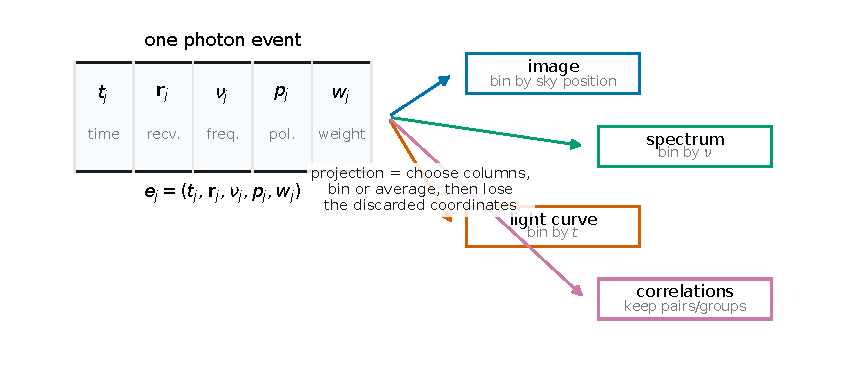
\includegraphics[width=0.9\linewidth]{figures/generated/chapter_01/ch01_event_table_map.pdf}
\caption{The same photon event list can be projected into many kinds of data products. Binning along position gives an image, binning along frequency gives a spectrum, binning along time gives a light curve, and combining across polarization channels gives the polarization quantities. Every projection preserves part of the information and discards part; relationships such as ``how photons arrive together in pairs'' become visible only when one returns to the raw event list.}
\label{fig:e00-event-map}
\end{figure}

\section{Light Speaks Two Languages: Wave, and Count}
\label{sec:e00-two-languages}

To read what has been ``thrown away'' in the event list, you must first accept something that physicists argued about for a century: \textbf{light speaks two languages at once}, and the two languages describe one and the same thing.

The first is the \textbf{language of the wave}. Within a sufficiently narrow band of colour, light can be regarded as a train of oscillating electromagnetic waves: what is really trembling is the electric field, which has an amplitude, a phase, and interferes. Superpose two beams: crest on crest is brighter, crest on trough is dimmer: this is constructive and destructive interference. Phase, interference, fringes are the keywords of this language. The electric field of visible light must oscillate hundreds of trillions of times per second, one period lasting only a few femtoseconds (\(\mathrm{fs}=10^{-15}\,\mathrm{s}\)), too fast for any ordinary detector to keep up with; and so the detector cannot see the positive and negative swings of the field, and can only smooth these rapid oscillations over its own response time, leaving in the end only the energy.

The second is the \textbf{language of counting}. What the detector leaves behind is a set of discrete ``clicks,'' each one the tap of a single photon. Since these are independent random taps one after another, the count must inevitably carry fluctuations: even if the source brightness, the telescope, and the detector all hold perfectly still, the number of photons you count each millisecond will still jitter up and down. This inborn jitter is called \textbf{shot noise} (also called Poisson noise); it is not a flaw of the instrument, but the inevitable shadow of the fact that ``light really is counted out one grain at a time.''

These two languages sound like polar opposites (one speaks of continuous waves and phase, the other of discrete taps and probability), but the whole charm of quantum astronomy lies in the fact that they are two faces of the same coin, and can both be read out of the \textbf{event list}. Here I will only give a preview, planting three threads:

\begin{itemize}
  \item The language of the wave (electric field, complex amplitude, phase, interference) will be formally taken up in Chapter~\ref{chap:e01}, where we will write the electric field as a ``rotating arrow''; Chapter~\ref{chap:e02} then extends it through Fourier analysis, making clear the notions of bandwidth and coherence time, that is, ``how long can this arrow remember its own phase.''
  \item The language of counting (probability, Poisson statistics, shot noise) will be worked out in Chapter~\ref{chap:e03}, where we go from the most naive picture of ``slice time into many little cells'' all the way to the Poisson distribution, computing the fluctuation of the ``clicks'' as a predictable number.
  \item With these two languages in hand, we must first make the ``photon'' itself rigorous: Chapter~\ref{chap:e04} supplies the ladder operators of quantum mechanics and the harmonic oscillator, and Chapter~\ref{chap:e05} uses them to give the quantization of light. Only this is the thread and needle that truly sews ``wave'' and ``count'' into one and the same mathematics.
  \item And the bridge that welds these two languages fully together, that turns ``coherence of the wave'' directly into ``correlation of the counts,'' intensity interferometry and the Hanbury Brown--Twiss (HBT) effect, belongs to Part 2 of the book, ``Coherence and Correlation.'' It is only there, in chapters even later than the quantization of light, that it is formally erected.
\end{itemize}

In other words, the suspense this chapter has planted (``how a single batch of photons arrives together, and what is hidden in that'') can only be fully explained when the two languages are joined. Chapters~\ref{chap:e01} through~\ref{chap:e05} first sharpen each of the two languages on its own and make the ``photon'' rigorous; the HBT correlation that truly brings the two together is left for the later part on ``Coherence and Correlation'' to reel in.

\section{The Promise of This Book: Why It Is Worth Learning This ``Quantum'' Language}
\label{sec:e00-promise}

You might ask: traditional astronomy can already deliver images, spectra, light curves, and polarization, and gets along just fine, so why go to the trouble of learning this ``quantum'' language of returning to the event list and watching how photons arrive together? Because it can do some things that traditional methods \textbf{cannot do in principle}. This is not treating ``quantum'' as a gimmick, but a matter of real scientific returns.

\textbf{Measuring the true size of a star.} Stars are so far away that in a telescope they are almost all just a point. Their angular diameters are as small as the milliarcsecond (mas, i.e.\ \(10^{-3}\) arcsecond) or even the microarcsecond. How small is that? \(1\,\mathrm{mas}\approx4.85\times10^{-9}\,\mathrm{rad}\); to make a coin about \(2.5\,\mathrm{cm}\) in diameter subtend such a small angle, you would have to place it about five thousand kilometres away, roughly half the distance from Beijing to London; and a microarcsecond is another thousand times smaller. An ordinary telescope, limited by the diffraction limit, simply cannot resolve such fine angular structure, but intensity interferometry can correlate the photon counts of two telescopes a hundred metres or a kilometre apart, and from ``how synchronized the fluctuations of the two telescopes are'' infer this angular diameter. A star is no longer a point, but acquires a measurable disk, a shape flattened by rotation, and limb darkening at its edge.

\textbf{Approaching the edges of black holes and compact objects.} Longer baselines and higher time resolution can in principle push this method toward smaller angular scales, to constrain accretion disks, stellar winds, and even the structure around compact objects.

\textbf{Putting new physics on a leash.} The extremely precise measurement of photon arrival times and correlations can also be used to test ideas beyond the Standard Model. Any question that can be written as ``an estimable quantity in the event list $+$ an honest error budget $+$ a null test'' may become a genuinely executable observing program.

These are not idle words on paper. Please remember three real names, which will recur throughout the book:

\begin{itemize}
  \item \textbf{Narrabri}: in the 1960s, the stellar intensity interferometer at Narrabri, Australia, used two large reflectors that could slide along a track to systematically measure, for the first time, the angular diameters of dozens of bright stars. This is the starting point of the craft.
  \item \textbf{VERITAS} and \textbf{MAGIC}: today, large Cherenkov telescope arrays (each more than ten metres in aperture) originally built to catch high-energy gamma rays have been cleverly repurposed as optical intensity interferometers, measuring the sub-milliarcsecond angular diameters of bright stars to a precision of a few percent. A method that lay dormant for years because its signal was too weak has, thanks to large mirrors, fast electronics, and digital correlators, come back to life.
\end{itemize}

Figure~\ref{fig:e00-science-map} places these science goals on the same map: read horizontally it is ``how close to conventional observation,'' read vertically it is ``how much new information beyond the reach of traditional methods.'' The angular diameters of bright stars are already within arm's reach, while farther out lie goals of extremely high value that demand more engineering breakthroughs, such as supernova distance measurement and the quantum-network telescope. This figure is the territory the book wishes to invite you to explore together.

\begin{figure}[tbp]
\centering
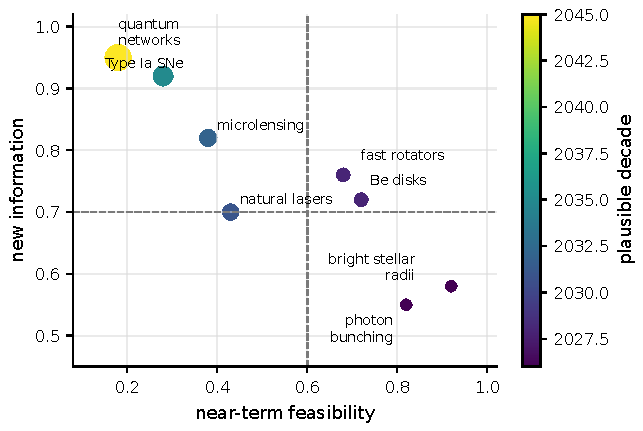
\includegraphics[width=0.8\linewidth]{figures/generated/chapter_02/ch02_science_case_map.pdf}
\caption{A map of the first-generation science questions of quantum astronomy: the horizontal axis roughly indicates distance from conventional observation, and the vertical axis indicates the amount of information gained relative to traditional methods. The angular diameters of bright stars and stellar photon bunching are already close to present capability; fast rotators, stellar disks, and natural masers are near-term extensions; supernova angular-distance measurement and the quantum-network telescope are of the highest value but require engineering breakthroughs such as longer baselines, fast triggering, or quantum links.}
\label{fig:e00-science-map}
\end{figure}

\section{A Map of the Whole Book: The Seven Stops We Will Travel Together}
\label{sec:e00-map}

Finally, let us unroll the whole map. The book is divided into seven parts (Part 0 through Part 6), like a construction route that builds from the foundation all the way up to the roof. You need not read it all in one go, but you had best know which storey each stop is building:

\begin{itemize}
  \item \textbf{Part 0: Foundations and languages.} These are the very chapters you are reading. We hone two tools: the language of the wave (electric field, complex amplitude, phase, interference) and the language of counting (Poisson statistics, shot noise, order-of-magnitude estimation). The goal is that whenever you meet a formula, you first see the physical picture behind it.
  \item \textbf{Part 1: The quantum description of light.} Making the word ``photon'' rigorous: from the quantization of the electric field to the coherent state, the thermal state, and the number state, understanding why laser-like coherent light and star-like thermal light differ so profoundly in ``how their photons arrive together.''
  \item \textbf{Part 2: Coherence and correlation.} The heart of the book. First-order coherence \(g^{(1)}\) (interference, visibility) and second-order coherence \(g^{(2)}\) (photon bunching, intensity correlation) make their entrance here, the Siegert relation welds the two together, and the HBT effect turns from a ``bizarre phenomenon'' into ``computable physics.''
  \item \textbf{Part 3: From correlation to imaging.} The van Cittert--Zernike theorem tells us how the brightness distribution of the sky is encoded into the spatial coherence; and so ``the correlation of two telescopes'' is translated into ``the angular diameter of a star,'' and the principle of intensity-interferometric imaging closes the loop here.
  \item \textbf{Part 4: The limits of measurement.} Introducing Fisher information and the Cramér--Rao lower bound to answer an honest question: given so many photons and so long an integration time, how precisely can we \textbf{at best} measure the angular diameter? The noise budget is laid on the table here.
  \item \textbf{Part 5: Real instruments and observations.} The atmosphere, detector jitter, dead time, background, clock synchronization, the \(u,v\) coverage of multiple telescopes: bringing the ideal formulas down into the mud of real systems such as Narrabri, VERITAS, and MAGIC.
  \item \textbf{Part 6: Frontiers and outlook.} Frequency and polarization correlations, natural masers, microlensing, quantum-enhanced measurement, and the quantum-network telescope, pushing the boundary of the map toward regions still under exploration.
\end{itemize}

\textbf{How should this book be used?} If you are an undergraduate, please read in order, and treat every formula annotated with a small \verb|formulaexplain| note as a ``prompt card'': first read the physical picture in the main text, then go back and check the unit and meaning of every symbol; when you meet a derivation, do not skip steps: the book has already written out every intermediate step, and all you need to do is walk through it once. If you already have a background, you may jump straight to \(g^{(2)}\) in Part 2 and the information limits in Part 4, which is where the book's information density is highest. However you enter, remember to glance back at this map from time to time and ask yourself: \emph{which stop am I standing at now, and which storey is the tool in my hand meant to build?}

\section{Chapter Summary}
\label{sec:e00-summary}

\begin{itemize}
  \item A telescope stores neither the wave nor an image, but a labelled \textbf{photon event list}, each row being \(e_j=(t_j,\bm r_j,\nu_j,p_j,w_j)\): time, position, frequency channel, polarization/electronics channel, and quality weight.
  \item Images, spectra, light curves, and polarization quantities are all \textbf{projections} of this list along different columns; every projection preserves part of the information and discards part, while ``how photons arrive together in pairs'' is visible only in the raw event list.
  \item Light speaks both the \textbf{language of the wave} (electric field, phase, interference) and the \textbf{language of counting} (taps, Poisson noise); Chapters~\ref{chap:e01} through~\ref{chap:e03} sharpen each of these two languages (wave and coherence time in Chapters~\ref{chap:e01} and~\ref{chap:e02}, Poisson and shot noise in Chapter~\ref{chap:e03}), and Chapters~\ref{chap:e04} and~\ref{chap:e05} then make the ``photon'' rigorous; the HBT correlation that truly brings the two together is left for Part 2, ``Coherence and Correlation,'' to reel in.
  \item The reward for learning this language is tangible: \textbf{stellar angular diameters} at the milliarcsecond and even microarcsecond level, the edges of compact objects, and constraints on new physics; Narrabri, VERITAS, and MAGIC have already turned it from concept into measurement.
\end{itemize}

\medskip
\noindent\textbf{Questions to Ponder.}
\begin{itemize}
  \item If you were allowed to keep only \textbf{one column} of the event list, which column would you keep? To answer ``how big is the star,'' which column can least afford to be lost?
  \item For the same stretch of observation, what does compressing it into an image throw away and keep, and what does compressing it into a light curve throw away and keep? Is there any kind of information that neither projection can retain?
  \item ``Shot noise'' is not a defect of the instrument but the inevitable consequence of light being counted one grain at a time. So if you double the integration time, roughly what fraction of its original value does the relative fluctuation become? (Hint: think about \(1/\sqrt{\mu}\).)
\end{itemize}

\chapter{Waves, Phase, and Complex Amplitude: The Minimal Language of Interference}
\label{chap:e01}

\begin{chapteropening}
Imagine you are standing behind the focus of a telescope, and a beam of starlight has just fallen in. What is it, physically? It is a stretch of electric field swinging rapidly back and forth: how rapidly? One round trip takes only a few femtoseconds, trillions of times faster than a single blink of your eye. Yet when this light finally becomes data, that rapid swinging has ``vanished,'' and the detector leaves behind only a quiet number: the intensity, or the photon count. Where did the swinging go? Where did the phase go?

What this chapter sets out to do is to build up the ``language of the wave'' from the ground up: first we write down a stretch of monochromatic electromagnetic wave; then we learn to use a ``rotating arrow'' (the complex amplitude) to hold both its amplitude and its phase at once; then we work out why the detector can see only the square of the amplitude and not the phase itself; and finally we let two beams of light meet and watch how interference turns the ``invisible phase difference'' back into ``visible brightness and darkness.'' These few things are the shared alphabet of all the later chapters on coherence, interference, and intensity correlation.
\end{chapteropening}

\section{The Monochromatic Electromagnetic Wave: A Stretch of Rapidly Swinging Electric Field}
\label{sec:e01-wave}

Let us first set the picture. Within a sufficiently narrow frequency channel, starlight can be approximated as a train of \textbf{monochromatic light}: it has a single frequency, like a pure tone. What is really oscillating is the electric field strength at some point in space: it goes up and down with time, like a string that swings steadily after being plucked. Mathematically we write it as

\begin{equation}
  E(t)=E_0\cos(\omega t+\phi),\qquad \omega=2\pi\nu .
  \label{eq:e01-monochromatic}
\end{equation}
\begin{formulaexplain}
\(E(t)\) is the electric field at time \(t\); \(E_0\) is the amplitude (the maximum extent of the swing); \(\omega\) is the angular frequency, \(\nu\) is the ordinary frequency, and the two differ by a factor of \(2\pi\); \(\phi\) is the initial phase, which sets where the swing is at \(t=0\).
\end{formulaexplain}

Let us pin down each symbol. \(E(t)\) is the electric field; in CGS units its dimension is \({\rm statvolt\,cm^{-1}}\), but for the derivations of this chapter its actual magnitude does not matter: what matters is \emph{how it varies with time}. \(E_0\) is the maximum height of this swing, that is, the amplitude, which likewise carries the dimension of electric field. \(\phi\) is the initial phase, in units of radians; it is a pure angle and dimensionless, and you can read it as ``at the instant \(t=0\), how far into the cycle the swing has progressed.''

The quantity \(\omega t+\phi\) inside the parentheses is called the \textbf{instantaneous phase}: as time passes, \(\omega t\) increases uniformly, and the cosine swings again and again from \(+1\) down to \(-1\) and back. The unit of the angular frequency \(\omega\) is \({\rm rad\,s^{-1}}\); it tells us how fast the phase advances. Its relation to the ordinary frequency \(\nu\) (in Hz, that is, how many full cycles per second) is \(\omega=2\pi\nu\), because one full turn is \(2\pi\) radians. The period is \(T=1/\nu=2\pi/\omega\).

Now let us put in real numbers to feel how fast this is. Visible light has a frequency of about

\[
  \nu\simeq 4\times10^{14}\ {\rm Hz}\ (\text{red light})\quad\text{to}\quad 8\times10^{14}\ {\rm Hz}\ (\text{blue light}),
\]

so one period is only

\[
  T=\frac{1}{\nu}\simeq\frac{1}{5\times10^{14}\ {\rm Hz}}=2\times10^{-15}\ {\rm s}=2\ {\rm fs}.
\]

That is, the electric field of visible light completes one full up-and-down swing every two femtoseconds. What kind of a scale is a femtosecond (\(10^{-15}\) second)? In one femtosecond, light travels only \(0.3\ \mu{\rm m}\), less than a hundredth of the diameter of a human hair. Any conventional astronomical detector, whether a CCD pixel, a photomultiplier tube, or an avalanche photodiode, has a response time of at least the nanosecond (\(10^{-9}\) second) scale, \(10^{5}\)--\(10^{6}\) times slower than one optical period (comparing ``at least \(1\ {\rm ns}\)'' with ``about \(2\ {\rm fs}\)'' gives \(1\ {\rm ns}/2\ {\rm fs}\approx5\times10^{5}\); for a CCD with integration times down to the microsecond scale it is slower still).

This brings out a key fact that runs through the whole book: the detector is ``too slow'': it simply cannot keep up with the field's cycle-by-cycle positive and negative swings. In the time it takes the detector to blink its ``electronic eye'' once, the field has already swung up and down hundreds of thousands or even millions of times. It cannot record each swing; it can only \emph{smooth} these rapid oscillations over its own response time, leaving behind an average energy. So the rapidly varying part of \(E(t)\), the part carrying the phase information, is \textbf{directly invisible} to the detector. We will see later that it is precisely this that forces people to invent interferometry and correlation measurements: the only way to turn the ``invisible phase'' back into ``visible intensity.''

\section{Complex Amplitude: Packing Amplitude and Phase into One Rotating Arrow}
\label{sec:e01-phasor}

Equation~\eqref{eq:e01-monochromatic} is a bit clumsy: every time we discuss adding two beams together and how the phase difference changes, we have to fiddle with a pile of product-to-sum cosine formulas. Is there a cleverer notation that packs the two things, \emph{amplitude} and \emph{phase}, in one stroke, and also makes addition simple? Yes: this is the \textbf{complex amplitude} (also called a phasor).

First the picture. Think of the cosine as the projection onto the horizontal axis of an arrow that starts at the origin and rotates uniformly about it: the \emph{length} of the arrow is the amplitude \(E_0\), and the \emph{angle} the arrow points to is the instantaneous phase \(\omega t+\phi\). The arrow turns counterclockwise at angular velocity \(\omega\)\footnote{Here we have chosen the \(e^{+i\omega t}\) time convention: the arrow rotates counterclockwise, and positive frequencies take \(+i\omega t\). Within this chapter it is entirely self-consistent, and none of the conclusions are affected. One reminder, to avoid confusion when interfacing later: when we introduce the positive/negative-frequency field operators \(\hat E^{(+)},\hat E^{(-)}\) for second quantization, the positive-frequency part \(\hat E^{(+)}\) containing the annihilation operator \(\hat a\) usually evolves as \(e^{-i\omega t}\), so the arrow turns the opposite way from here. The two conventions are just mirror-image notations for the same physics: replacing every \(i\) here with \(-i\) (equivalent to viewing the arrow as turning clockwise) interfaces smoothly, with the physical content unchanged.}, and its shadow on the real axis (the horizontal direction) is exactly \(E_0\cos(\omega t+\phi)\). So ``a stretch of oscillating field'' is translated into ``a rotating arrow.'' Since we want to describe an arrow in the plane, complex numbers are the most natural choice: a point in the complex plane inherently carries the two pieces of information ``length'' and ``angle.''

We package the arrow's appearance at \(t=0\) (length \(E_0\), angle \(\phi\)) into a complex number:

\begin{equation}
  \mathcal{E}=E_0e^{i\phi},\qquad E(t)=\operatorname{Re}\!\left[\mathcal{E}\,e^{i\omega t}\right].
  \label{eq:e01-phasor}
\end{equation}
\begin{formulaexplain}
\(\mathcal E\) is the complex amplitude; its modulus \(|\mathcal E|=E_0\) is the amplitude, and its argument \(\arg\mathcal E=\phi\) is the phase. Multiplying by the rotation factor \(e^{i\omega t}\) sets the arrow turning, and taking the real part \(\operatorname{Re}\) (the horizontal shadow) recovers the real electric field \(E(t)\).
\end{formulaexplain}

Let us verify that this notation really recovers Eq.~\eqref{eq:e01-monochromatic}. Using Euler's formula \(e^{i\theta}=\cos\theta+i\sin\theta\) (this is the definition of the complex exponential, which the book will use again and again), we expand step by step:

\[
  \mathcal{E}\,e^{i\omega t}
  =E_0e^{i\phi}\,e^{i\omega t}
  =E_0\,e^{i(\omega t+\phi)}
  =E_0\bigl[\cos(\omega t+\phi)+i\sin(\omega t+\phi)\bigr].
\]

Taking the real part (discarding the imaginary part carrying \(i\)):

\[
  \operatorname{Re}\!\left[\mathcal{E}\,e^{i\omega t}\right]
  =E_0\cos(\omega t+\phi)=E(t).
\]

Not a step off: exactly the original field. So no information is lost in the complex amplitude \(\mathcal E\): \(|\mathcal E|=|E_0e^{i\phi}|=E_0\) gives the amplitude, and \(\arg\mathcal E=\phi\) gives the phase. \(\mathcal E\) carries the same dimension as the electric field, while the \(e^{i\phi}\) part is a dimensionless pure direction.

The advantage of this notation only truly shows itself in the next section, when two beams are added: adding cosines is troublesome, but adding complex numbers is just vector addition of arrows placed head to tail, much simpler. This is why, from now on, we almost always do our bookkeeping first in the world of complex amplitudes, and only take the real part or the modulus at the end to fall back into the real world.

\section{Intensity: Why the Detector Sees Only the Square of the Amplitude}
\label{sec:e01-intensity}

Back to the core question: the detector cannot see the rapid swinging, so what exactly does it record? The answer is the \textbf{intensity}, that is, the average of the square of the field over the response time. Physically, the detector absorbs the energy of the light, and the energy density carried by the electromagnetic field is proportional to the square of the field. So the quantity left behind by the detector is proportional to \(\langle E^2(t)\rangle\), where the angle brackets denote ``a time average over the detector's response time.''

Let us compute this average step by step, skipping nothing. Starting from \(E(t)=E_0\cos(\omega t+\phi)\):

\[
  E^2(t)=E_0^2\cos^2(\omega t+\phi).
\]

The key step is to use the double-angle identity for the cosine, \(\cos^2\theta=\tfrac12\bigl[1+\cos(2\theta)\bigr]\) (a standard trigonometric identity, obtainable by solving \(\cos 2\theta=2\cos^2\theta-1\)), to split the square open:

\[
  E^2(t)=E_0^2\cdot\frac{1+\cos\!\bigl(2\omega t+2\phi\bigr)}{2}
  =\frac{E_0^2}{2}+\frac{E_0^2}{2}\cos\!\bigl(2\omega t+2\phi\bigr).
\]

Now take the time average. The first term on the right, \(E_0^2/2\), is a constant, and its average is itself. The second term is a cosine oscillating rapidly at \(2\omega\) (twice the optical frequency, an even shorter period): over the detector's long response time it swings up and down through countless full periods, the positive parts and the negative parts cancelling exactly, so its average is zero. This is precisely the ``smoothing'' spoken of in the previous section:

\[
  \bigl\langle\cos(2\omega t+2\phi)\bigr\rangle_{\rm det}\approx 0
  \quad\Longrightarrow\quad
  \bigl\langle E^2(t)\bigr\rangle_{\rm det}=\frac{E_0^2}{2}.
\]

So the intensity left behind by the detector is proportional to

\begin{equation}
  I\ \propto\ \bigl\langle E^2(t)\bigr\rangle_{\rm det}=\frac{E_0^2}{2}=\frac{1}{2}\,|\mathcal E|^2 .
  \label{eq:e01-intensity}
\end{equation}
\begin{formulaexplain}
\(I\) is the detected intensity; \(\langle\cdots\rangle_{\rm det}\) is the time average over the detector's response time; that \(1/2\) is precisely the result of averaging \(\cos^2\) over one period; \(|\mathcal E|^2\) is the modulus squared of the complex amplitude. The phase \(\phi\) has \emph{vanished} from the final result.
\end{formulaexplain}

Please stare especially hard at what disappears at the end of this equation: \(\phi\) is gone. The intensity depends only on the amplitude \(E_0\) (or \(|\mathcal E|\)), and not at all on the phase. From the complex-amplitude viewpoint this is even more transparent: \(|\mathcal E|^2=|E_0e^{i\phi}|^2=E_0^2\), the modulus of that \(e^{i\phi}\) is 1, and taking the modulus squared swallows the phase factor entirely. No matter which direction the rotating arrow initially points, as long as its length is the same, the measured intensity is the same.

Physically this sentence is a cornerstone of the whole book: \textbf{the phase of a single beam of light is not directly recorded by the detector}. It is like a hidden degree of freedom; the intensity data in your hands know nothing about it. But earlier chapters said the phase is important. Isn't this a contradiction? It is not: the absolute phase of a single beam really cannot be measured, but the \emph{phase difference} of two beams can, because the phase difference changes the length of the resultant arrow, and thereby changes the intensity. This is exactly where interference comes into play, and we go to see it right away.

(A notational convention: that constant \(1/2\), along with various geometrical and efficiency factors, is often absorbed into the proportionality constant in later text and written as \(I\propto|\mathcal E|^2\). This chapter writes the \(1/2\) out explicitly to make the step of ``smoothing away the rapid oscillation'' plain to see.)

\section{When Two Beams Meet: How Interference Turns a Phase Difference Back into Brightness and Darkness}
\label{sec:e01-interference}

Now let two beams of monochromatic light (say, from the same star, having taken two different paths) fall on the same detector. The crucial physical order is: \textbf{the fields are added first, and the intensity is squared afterward}. This order cannot be reversed. Because the electromagnetic field obeys the superposition principle, the fields of the two beams at the same point add as vectors; and what the detector measures is the energy of that resultant field \emph{after} the addition. Doing this with complex amplitudes is the least laborious: two arrows head to tail, mere vector addition.

Let the complex amplitudes of the two beams be \(\mathcal E_1\) and \(\mathcal E_2\); the complex amplitude of the resultant field is then \(\mathcal E_1+\mathcal E_2\). The intensity is proportional to its modulus squared:

\begin{equation}
  I\ \propto\ |\mathcal E_1+\mathcal E_2|^2
  =|\mathcal E_1|^2+|\mathcal E_2|^2+2\,\operatorname{Re}\!\bigl(\mathcal E_1\mathcal E_2^{\ast}\bigr).
  \label{eq:e01-interference}
\end{equation}
\begin{formulaexplain}
\(\mathcal E_1,\mathcal E_2\) are the complex amplitudes of the two beams; the first two terms \(|\mathcal E_1|^2,|\mathcal E_2|^2\) are their separate intensities; the third term \(2\operatorname{Re}(\mathcal E_1\mathcal E_2^{\ast})\) is the \emph{interference term}, where the star \({}^\ast\) denotes complex conjugation. It is this term that makes the total intensity larger or smaller.
\end{formulaexplain}

Let us derive this expansion honestly. For any complex number \(z\), the modulus squared is it times its own conjugate: \(|z|^2=z\,z^{\ast}\). Let \(z=\mathcal E_1+\mathcal E_2\); its conjugate is \(\mathcal E_1^{\ast}+\mathcal E_2^{\ast}\), and multiplying term by term:

\[
  |\mathcal E_1+\mathcal E_2|^2
  =(\mathcal E_1+\mathcal E_2)(\mathcal E_1^{\ast}+\mathcal E_2^{\ast})
  =\mathcal E_1\mathcal E_1^{\ast}+\mathcal E_2\mathcal E_2^{\ast}
  +\mathcal E_1\mathcal E_2^{\ast}+\mathcal E_2\mathcal E_1^{\ast}.
\]

The first two terms are \(|\mathcal E_1|^2\) and \(|\mathcal E_2|^2\). The last two terms, \(\mathcal E_1\mathcal E_2^{\ast}\) and \(\mathcal E_2\mathcal E_1^{\ast}\), are conjugates of each other, and since ``a complex number plus its conjugate equals twice its real part'' (\(z+z^{\ast}=2\operatorname{Re}z\)), together they are precisely \(2\operatorname{Re}(\mathcal E_1\mathcal E_2^{\ast})\). This gives Eq.~\eqref{eq:e01-interference}.

Next, let us substitute the explicit form of the complex amplitude to make the phase appear. Writing \(\mathcal E_1=E_1e^{i\phi_1}\) and \(\mathcal E_2=E_2e^{i\phi_2}\), first compute the product:

\[
  \mathcal E_1\mathcal E_2^{\ast}
  =E_1e^{i\phi_1}\cdot E_2e^{-i\phi_2}
  =E_1E_2\,e^{i(\phi_1-\phi_2)}
  =E_1E_2\bigl[\cos(\phi_1-\phi_2)+i\sin(\phi_1-\phi_2)\bigr].
\]

Taking the real part and discarding the imaginary part, the interference term becomes

\[
  2\,\operatorname{Re}\!\bigl(\mathcal E_1\mathcal E_2^{\ast}\bigr)
  =2E_1E_2\cos(\phi_1-\phi_2).
\]

So the total intensity of the two beams is written as

\[
  I\ \propto\ E_1^2+E_2^2+2E_1E_2\cos(\phi_1-\phi_2).
\]

Look at the last term of this equation: it depends only on the \textbf{phase difference} \(\Delta\phi=\phi_1-\phi_2\), not on the individual absolute phases. This is exactly what echoes the conclusion of the previous section: the absolute phase cannot be measured, but the phase difference can be made manifest through the intensity. Read it in three cases:

\begin{itemize}
  \item \textbf{Constructive interference}: \(\Delta\phi=0\) (or an integer multiple of \(2\pi\)), \(\cos\Delta\phi=+1\), and the interference term takes its maximum positive value. The two arrows superpose in the same direction, the resultant arrow is longest, and the intensity surges to the peak \(E_1^2+E_2^2+2E_1E_2=(E_1+E_2)^2\). If \(E_1=E_2=E_0\), the peak is \(4E_0^2\), \emph{four} times the single-beam intensity \(E_0^2\), not twice. The extra energy is precisely the result of interference ``redistributing'' it.
  \item \textbf{Destructive interference}: \(\Delta\phi=\pi\), \(\cos\Delta\phi=-1\), and the interference term takes its maximum negative value. The two arrows point in opposite directions, the resultant arrow is shortest, and the intensity drops to the trough \((E_1-E_2)^2\). For equal intensities \(E_1=E_2\), it is \emph{completely dark} here.
  \item \textbf{Averaged away}: if the phase difference \(\Delta\phi\) is unstable, varying rapidly and irregularly over the measurement time (the two beams cannot ``remember'' each other's phase), then \(\cos\Delta\phi\) is now positive, now negative, averaging toward zero, the interference term vanishes, and only \(I\propto E_1^2+E_2^2\) remains: the two beams add simply, like incoherent street lamps. This question of ``whether the phase difference stays stable'' is precisely \textbf{coherence}, which is the protagonist of the whole book from Chapter~\ref{chap:e05} onward.
\end{itemize}

To close this section in one sentence: interference is a ``phase-difference translation machine'': it translates the phase difference \(\Delta\phi\), which the detector cannot see, into visible brightness and darkness (the highs and lows of the intensity). All the various interference and correlation measurements discussed in this book are, at heart, reading out this \(\cos\Delta\phi\) with different tricks.

\begin{figure}[tbp]
\centering
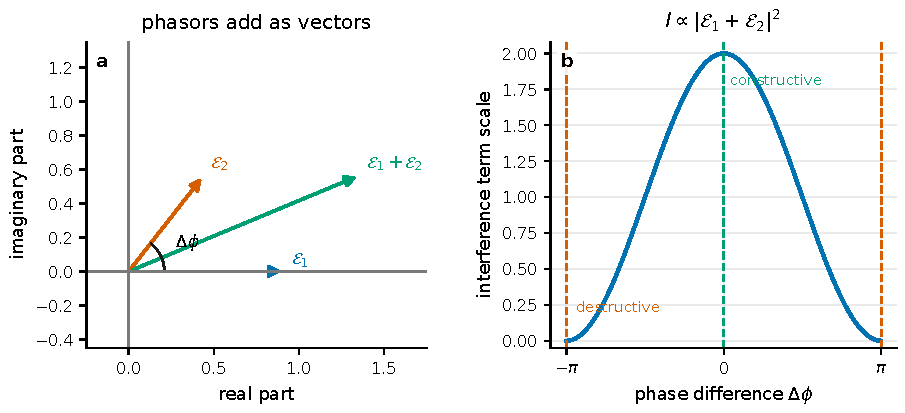
\includegraphics[width=0.85\linewidth]{figures/generated/chapter_01/ch01_phase_interference.pdf}
\caption{The basic picture of complex amplitudes and the interference of two beams. The complex amplitude is an arrow whose length is the amplitude and whose direction is the phase; the two beams first undergo vector addition of the arrows, and the detector then takes the square of the length of the resultant arrow. The phase difference \(\Delta\phi\) determines whether the interference term reinforces (constructive), cancels (destructive), or is averaged away when the phase varies wildly.}
\label{fig:e01-phase-interference}
\end{figure}

\section{Geometric Phase: Where the Path Difference Comes From}
\label{sec:e01-geometry}

The phase difference \(\Delta\phi\) of the previous section is still rather abstract. In astronomical observation, its most common source is in fact very concrete and very geometric: \textbf{the two beams travel paths of unequal length}. This section turns this ``path difference'' step by step into a phase difference.

First set the picture. Let there be a very distant star; when the light it emits reaches the ground, the wavefront (the surface of equal phase) is almost a large flat sheet, advancing along the source direction \(\bm s\) (a unit vector pointing to the star). On the ground there are two telescopes, whose positions differ by a \textbf{baseline vector} \(\bm B\), the vector pointing from the first to the second, in units of centimetres. Because the two telescopes are not on the same wavefront perpendicular to \(\bm s\), one and the same wavefront reaches one of them first and must travel a little extra to reach the other. This ``little extra'' is the path difference.

How long is the extra path? Just project the baseline \(\bm B\) onto the source direction \(\bm s\). The length of the projection of a vector onto a given direction is precisely the dot product, so the path difference is

\[
  \Delta \ell=\bm B\cdot\bm s .
\]

The geometric meaning of this step must be seen clearly: \(\bm B\cdot\bm s=|\bm B|\cos\theta\), where \(\theta\) is the angle between the baseline and the source direction. If the star lies straight ahead of the baseline (\(\bm B\) parallel to \(\bm s\)), the projection is longest and the path difference greatest; if the star lies straight above the baseline (\(\bm B\perp\bm s\)), the projection is zero, the two telescopes have equal paths to the same wavefront, and there is no path difference. This agrees with everyday experience: only for light arriving at a slant is there a lead-and-lag between the two receiving points.

Now let us convert ``the extra stretch of path'' into ``the extra amount of phase turned.'' Here we need a fact that has not yet been formally stated, but that can be derived from the picture of Section~\ref{sec:e01-wave} right away: as the wave advances by one \textbf{wavelength} \(\lambda\) in space, the phase advances by exactly \(2\pi\) (one full turn). Why? Return to the time picture set up in Section~\ref{sec:e01-wave}: each time the field passes one period \(T\), the instantaneous phase increases by \(\omega T=2\pi\) (this is precisely the definition of ``one full turn per period''). And in that same time \(T\), a wave propagating at the speed of light \(c\) advances exactly a distance

\[
  \lambda\ \equiv\ cT=\frac{c}{\nu}=\frac{2\pi c}{\omega}.
\]

The spatial length corresponding to this ``phase accumulating exactly one full turn of \(2\pi\)'' is the wavelength. So ``one period has passed in time'' and ``one wavelength has been advanced in space'' are two ways of saying the same thing, with the phase advancing by exactly \(2\pi\) in both. In this way, \(\lambda\) is not a new symbol appearing out of nowhere: it is directly determined from the \(\nu\) (or \(\omega\)) honed repeatedly in Section~\ref{sec:e01-wave} through \(\lambda=c/\nu\). Substituting the visible-light frequency \(\nu\simeq5\times10^{14}\ {\rm Hz}\) from there, we get \(\lambda=c/\nu\approx(3\times10^{10}\ {\rm cm\,s^{-1}})/(5\times10^{14}\ {\rm Hz})=6\times10^{-5}\ {\rm cm}=0.6\ \mu{\rm m}\), exactly the visible-light wavelength we are familiar with, and self-consistent with the figure in Section~\ref{sec:e01-wave} that ``light travels \(0.3\ \mu{\rm m}\) in one femtosecond'' (two femtoseconds per period, exactly \(0.6\ \mu{\rm m}\) per wavelength).

With this ``exchange rate'' of ``one wavelength converts to \(2\pi\),'' the path difference is easy to convert: since advancing by one \(\lambda\) turns the phase by an extra \(2\pi\), advancing by \(\Delta\ell\) means advancing by \(\Delta\ell/\lambda\) wavelengths, so the phase advances by \(\Delta\ell/\lambda\) turns, that is, \(2\pi\times(\Delta\ell/\lambda)\) radians. Substituting \(\Delta\ell=\bm B\cdot\bm s\):

\begin{equation}
  \Delta\phi=\frac{2\pi}{\lambda}\,\bm B\cdot\bm s .
  \label{eq:e01-geometric-phase}
\end{equation}
\begin{formulaexplain}
\(\Delta\phi\) is the geometric phase difference of the two beams; \(\bm B\) is the baseline vector between the two receiving points; \(\bm s\) is the source-direction unit vector; \(\bm B\cdot\bm s\) is the projected path difference; the leading \(2\pi/\lambda\) is the conversion factor of ``each wavelength converts to \(2\pi\) of phase.''
\end{formulaexplain}

Let us point at each part once more to make sure the units line up. \(\bm B\cdot\bm s\) is a length, in centimetres; \(\lambda\) is also a length, in centimetres; dividing the two gives ``how many wavelengths were travelled,'' a dimensionless number; then multiplying by \(2\pi\) (radians per turn) gives the dimensionless phase difference \(\Delta\phi\), measured in radians. The dimensions match perfectly. That \(2\pi/\lambda\) is often written as the wavenumber \(k=2\pi/\lambda\), so we also write \(\Delta\phi=k\,\bm B\cdot\bm s\): its meaning is always ``the exchange rate that translates length into phase.''

Let us put in real numbers to feel how large this phase difference is. The classic apparatus of stellar intensity interferometry, the Narrabri stellar intensity interferometer, had a maximum baseline of about \(B\simeq188\ {\rm m}\) and a working wavelength of about \(\lambda\simeq0.44\ \mu{\rm m}\); today, when Cherenkov telescope arrays such as VERITAS and MAGIC do intensity interferometry, the baselines are likewise on the scale of a hundred metres or more. Taking a neat set of representative values \(B\sim100\ {\rm m}=10^{4}\ {\rm cm}\), \(\lambda\sim0.5\ \mu{\rm m}=5\times10^{-5}\ {\rm cm}\), when the baseline is almost straight on the source direction the path difference can be as large as \(\Delta\ell\sim B=100\ {\rm m}\), so

\[
  \frac{\Delta\ell}{\lambda}\sim\frac{10^{4}\ {\rm cm}}{5\times10^{-5}\ {\rm cm}}=2\times10^{8}\ (\text{wavelengths}),\qquad
  \Delta\phi=2\pi\,\frac{\Delta\ell}{\lambda}\sim1.3\times10^{9}\ {\rm rad}.
\]

A phase difference as high as a billion radians, more than two hundred million full turns! This brings out a basic fact of interferometry: the absolute phase difference itself is an astronomical number, and no one actually counts how many full turns it makes in all. What is really measured, and really cared about, is how many turns this enormous \(\Delta\phi\) \emph{changes by} as the Earth's rotation slowly turns the baseline \(\bm B\) relative to the source direction \(\bm s\), or as the source's position on the sky differs slightly, that is, how many periods the interference fringes \emph{move}. The absolute phase is an astronomical number; only the \emph{relative} motion of the fringes is the measurable, usable signal.

This equation looks simple, yet it is the entire starting point of interferometry: substituting it back into the \(2E_1E_2\cos(\Delta\phi)\) of the previous section, the interference brightness and darkness the telescope sees are directly hooked onto the baseline \(\bm B\) and the source direction \(\bm s\): rotate the Earth (changing the projection of \(\bm B\) relative to \(\bm s\)), or shift the source's position slightly, and the fringes move. Conversely, from how the fringes move, one can infer the fine structure of the source on the sky. But here we have only built up the most basic language of phase; the fuller spatial coherence relation between two telescopes is not formally developed until Chapter~\ref{chap:e05} and beyond.

\section{Chapter Summary}
\label{sec:e01-summary}

\begin{itemize}
  \item The physical substance of monochromatic light is a rapidly swinging electric field \(E(t)=E_0\cos(\omega t+\phi)\); the period of visible light is only a few femtoseconds, about a million times faster than any conventional detector, so the cycle-by-cycle oscillation and phase are \textbf{invisible} to the detector.
  \item The complex amplitude \(\mathcal E=E_0e^{i\phi}\) is a rotating arrow: its length \(|\mathcal E|=E_0\) is the amplitude, and its direction \(\arg\mathcal E=\phi\) is the phase. Taking the real part, \(E(t)=\operatorname{Re}[\mathcal E e^{i\omega t}]\), recovers the real field; the arrow notation turns ``adding fields'' into simple vector addition.
  \item The intensity \(I\propto\langle E^2\rangle_{\rm det}=\tfrac12|\mathcal E|^2\). That \(1/2\) comes from averaging \(\cos^2\) over one period; the rapid oscillation term is smoothed away, and \emph{the absolute phase of a single beam is not recorded}.
  \item Two beams: add the fields first, square afterward: \(I\propto|\mathcal E_1+\mathcal E_2|^2=|\mathcal E_1|^2+|\mathcal E_2|^2+2E_1E_2\cos(\phi_1-\phi_2)\). The interference term recognizes only the phase difference: \(\Delta\phi=0\) constructive, \(\Delta\phi=\pi\) destructive, and if the phase varies wildly it is averaged away. Interference translates the invisible phase difference into visible brightness and darkness.
  \item In astronomy the most common phase difference comes from the geometric path difference \(\Delta\phi=(2\pi/\lambda)\,\bm B\cdot\bm s\): \(\bm B\cdot\bm s\) is the projected path difference of the baseline onto the source direction, and \(2\pi/\lambda\) converts length into phase. It is the starting point of spatial coherence and interferometric imaging (Chapter~\ref{chap:e05}).
\end{itemize}

\vspace{0.5em}
\noindent\textbf{Questions to Ponder.}
(1) When two beams of equal intensity interfere constructively, the peak intensity is four times that of a single beam, so where does that ``extra energy'' come from, and where does it go?
(2) If the baseline \(\bm B\) of two telescopes is turned to be exactly perpendicular to the source direction \(\bm s\), what does the geometric phase difference \(\Delta\phi\) equal? What happens to the interference fringes then?
(3) Why do the two statements ``the absolute phase cannot be measured, but the phase difference can'' not contradict each other? Try to answer using only Eq.~\eqref{eq:e01-intensity} and Eq.~\eqref{eq:e01-interference}.

\chapter{Fourier, Bandwidth, and Coherence Time}
\label{chap:e02}

\begin{chapteropening}
In the previous chapter we regarded light as ``a rapidly rotating complex-amplitude arrow,'' and also conceded that the detector is too slow and can only record the intensity after it has been smoothed. But ``too slow'' relative to what, exactly? And how long can the phase of the light stay ordered before it scrambles? To answer these questions, we must first learn a universal language: any stretch of a wave, no matter how complicated, can be decomposed into a heap of pure single-frequency sinusoids, just as a chord can always be broken down into individual pure tones. This chapter first makes this ``tone-decomposition'' language (Fourier analysis) clear, then uses it to derive three quantities we will use again and again later: the bandwidth \(\Delta\nu\), the coherence time \(\tau_c\), and the autocorrelation and power spectrum that link the two. By the end you will understand why a nanosecond-scale time gate in fact packs hundreds or thousands of ``coherence times'' into it.
\end{chapteropening}

\section{Any Wave Is a Superposition of Pure Tones}
\label{sec:e02-fourier-idea}

Let us first build the picture. Imagine you hold a signal \(f(t)\) that varies with time: it could be the displacement of a violin string, or the electric field at some point on the detection surface. Fourier's insight is this: this signal is never ``one solid block,'' but the result of many sinusoids of different frequencies superposed together. The low-frequency sinusoids sketch out the broad outline, the high-frequency sinusoids fill in the sharp detail; add them up according to their respective ``weights'' and the original signal is recovered. This list of ``how much weight each frequency carries'' is called the \textbf{spectrum} of the signal.

First consider the most easily imagined case: the signal is periodic with period \(T\), that is, \(f(t+T)=f(t)\). In this case the allowed frequencies are not continuous but come rung by rung as harmonics: the fundamental frequency \(\nu_1=1/T\) and its integer multiples \(\nu_n=n/T\). The Fourier series says that such a periodic signal can be written as
\begin{equation}
  f(t)=\sum_{n=-\infty}^{+\infty} c_n\,e^{\,i\,2\pi\nu_n t},
  \qquad
  \nu_n=\frac{n}{T},
  \label{eq:e02-fourier-series}
\end{equation}
\begin{formulaexplain}
\(f(t)\) is the signal of period \(T\); \(\nu_n=n/T\) is the frequency of the \(n\)-th harmonic; the complex coefficient \(c_n\) is the ``weight'' this harmonic carries in the signal (containing both amplitude and phase). The whole equation says: a periodic signal is a sum of a stack of discrete pure tones.
\end{formulaexplain}
Here each term \(e^{i2\pi\nu_n t}\) is a ``unit arrow rotating uniformly at frequency \(\nu_n\),'' and the complex coefficient \(c_n\) sets how long the arrow is (amplitude) and where it initially points (phase). Since \(e^{i2\pi\nu_n t}\) is a dimensionless pure-phase factor, the dimension of the signal \(f(t)\) is carried entirely by the complex coefficients \(c_n\); the unit of \(\nu_n\) is the hertz (\({\rm Hz}={\rm s^{-1}}\)). To extract the weight of a particular harmonic, one need only ``beat time'' between the signal and that harmonic: integrate over one period, and orthogonality makes all the other harmonics cancel, leaving only the one term we want:
\[
  c_n=\frac{1}{T}\int_{0}^{T} f(t)\,e^{-\,i\,2\pi\nu_n t}\,dt .
\]
The key fact used here is that different harmonics are mutually orthogonal: \(\frac{1}{T}\int_0^T e^{i2\pi(m-n)t/T}\,dt=\delta_{mn}\) (when \(m=n\) the integrand is identically 1 and the integral gives 1; when \(m\neq n\) it is a complex exponential over one full period, whose positives and negatives cancel to give 0). This is the first ``known result'' we call upon by name, and we will use it again and again later.

Now imagine the period \(T\) growing longer and longer. The spacing of the harmonics \(\Delta\nu=\nu_{n+1}-\nu_n=1/T\) becomes denser and denser; when \(T\to\infty\), the signal is no longer periodic, and the rung-by-rung discrete frequencies merge into a continuous frequency axis. The step most easily skipped here is: where exactly did that normalization factor \(1/T\) in the series go? Making it clear requires only a small trick: in the synthesis formula \eqref{eq:e02-fourier-series}, attach to each term a ``frequency-spacing'' factor \(\Delta\nu\) (recall \(\Delta\nu=1/T\)), multiplying by one and dividing by one, leaving the equation unchanged:
\[
  f(t)=\sum_{n} c_n\,e^{\,i2\pi\nu_n t}
      =\sum_{n} \frac{c_n}{\Delta\nu}\,e^{\,i2\pi\nu_n t}\,\Delta\nu .
\]
This step changes nothing; it merely arranges the whole sum into the standard shape of a Riemann sum \(\sum_n g(\nu_n)\,\Delta\nu\): each term carrying the small slice of frequency width \(\Delta\nu\) it occupies. When \(T\to\infty\), \(\Delta\nu\to d\nu\), the Riemann sum converges to an integral, the discrete frequency \(\nu_n\) becomes a continuous variable \(\nu\), and the combination \(c_n/\Delta\nu\) in the parentheses converges to a continuous \textbf{spectral density}
\[
  \tilde f(\nu)\;=\;\frac{c_n}{\Delta\nu}\;=\;c_n\,T .
\]
So the fate of the \(1/T\) is settled: it did not vanish into thin air, but was absorbed by \(\Delta\nu=1/T\) into the integration measure \(d\nu\), at the cost that the spectral density \(\tilde f(\nu)\) is larger than the original series coefficient \(c_n\) by a full factor of \(T\) (this also lines up with the analysis formula: multiply both sides of \(c_n=\frac1T\int_0^T f\,e^{-i2\pi\nu_n t}dt\) by \(T\), the \(1/T\) on the right cancels exactly, and what remains is \(\tilde f(\nu)=\int f\,e^{-i2\pi\nu t}dt\)). In this way the sum \(\sum_n\) cleanly becomes the integral \(\int d\nu\), and we have passed from the Fourier series to the Fourier transform. We shall not fuss over the remaining mathematical details of convergence, keeping only this physical intuition: the spectrum of a non-periodic signal is continuous, every frequency may appear, each carrying its own weight. The Fourier transform pair is written
\begin{equation}
  \tilde f(\nu)=\int_{-\infty}^{+\infty} f(t)\,e^{-\,i\,2\pi\nu t}\,dt,
  \qquad
  f(t)=\int_{-\infty}^{+\infty} \tilde f(\nu)\,e^{+\,i\,2\pi\nu t}\,d\nu .
  \label{eq:e02-fourier-transform}
\end{equation}
\begin{formulaexplain}
The left equation ``decomposes'' the time signal \(f(t)\) into the spectrum \(\tilde f(\nu)\); the right equation ``recomposes'' the spectrum back into the signal. \(e^{\mp i2\pi\nu t}\) is a pure tone of frequency \(\nu\). Decomposition and recomposition are inverses of each other, with no gain or loss of information.
\end{formulaexplain}
The two equations are inverses of each other: the left (the analysis equation) is like using a row of tuned tuning forks to ``listen'' for how strong each frequency in the signal is, while the right (the synthesis equation) is like replaying those pure tones according to their weights and reassembling the original signal. Note that \(\tilde f(\nu)\) is generally complex: its modulus \(|\tilde f(\nu)|\) says how much weight this frequency carries, and its argument gives the phase of this frequency component. If the frequency axis is replaced by the wavelength axis, this is exactly the abstract version of the spectral-line curve a spectrograph spits out. When later in the book we speak of ``spectral-line width,'' ``filter bandwidth,'' and ``coherence function,'' the underlying machinery is always this pair of equations.

To sum up in one sentence: the Fourier transform is a ``decompose-and-recompose'' machine that translates ``varies with time'' into ``composed of which frequencies.'' Next we set it to its first genuinely useful task.

\section{The Finite-Length Wave Packet: The Shorter in Time, the Broader in Frequency}
\label{sec:e02-wavepacket}

Real light is never an infinitely long, perfectly single-frequency sinusoid. Each time an atom in a star emits, it radiates only an extremely short wave train before being interrupted by a collision; a filter, too, passes only a small band of frequencies. So what we always face is a \textbf{wave packet}: a stretch of oscillation with a beginning and an end, whose frequency is not perfectly single either. Hidden here is an iron law that runs through the whole book: \emph{the shorter a wave is in time, the broader it is in frequency}; conversely, to be extremely pure in frequency, the wave train must be extremely long.

Why? The intuition is this: an infinitely long perfect sinusoid needs only one frequency to describe, and its spectrum is a single needle. But once you ``cut it short'' (multiply it by an envelope of finite width), you have forcibly snuffed it out at both ends, and the very act of ``snuffing out'' requires additional frequency components to accomplish (just as sounding an extremely brief ``tap'' must call upon a very wide band of pitches). The shorter the wave train, the more abruptly it is snuffed, and the wider the frequencies needed. Written as an order-of-magnitude relation, this is the famous
\begin{equation}
  \Delta\nu\,\Delta t \;\gtrsim\; 1 ,
  \label{eq:e02-bandwidth-time}
\end{equation}
\begin{formulaexplain}
\(\Delta t\) is the temporal duration width of the wave packet, and \(\Delta\nu\) is its spread in frequency. Their product cannot be smaller than about 1: the narrower in time, the necessarily broader in frequency. This is a universal constraint of the Fourier transform, not an instrumental defect.
\end{formulaexplain}
In the formula the unit of \(\Delta t\) is the second and the unit of \(\Delta\nu\) is the hertz, so the product is dimensionless. Note that this is not the Heisenberg uncertainty principle but a purely classical wave property; the quantum-mechanical \(\Delta E\,\Delta t\gtrsim\hbar\) is merely its counterpart after multiplying by \(E=h\nu\). The ``\(\gtrsim\)'' in Eq.~\eqref{eq:e02-bandwidth-time} reminds us that it is an order-of-magnitude relation, with the precise coefficient depending on how ``width'' and the envelope shape are defined. Below we use an example that can be computed to the end to turn this inequality into an equality.

\paragraph{Explicit calculation for a Gaussian wave packet}

Take an oscillation modulated by a Gaussian envelope; writing it in complex form is the least laborious:
\[
  f(t)=e^{-\,t^{2}/(2\sigma_t^{2})}\;e^{\,i\,2\pi\nu_0 t}.
\]
Here \(\nu_0\) is the carrier frequency (about \(6\times10^{14}\,{\rm Hz}\) for visible light), and \(\sigma_t\) is the temporal width of the envelope (in seconds): \(|f|\) reaches its peak at \(t=0\) and decays to \(e^{-1/2}\) of the peak at \(|t|\sim\sigma_t\). Let us find its spectrum \(\tilde f(\nu)\). Substituting into the definition \eqref{eq:e02-fourier-transform}:
\[
  \tilde f(\nu)=\int_{-\infty}^{+\infty}
  e^{-\,t^{2}/(2\sigma_t^{2})}\,e^{\,i\,2\pi\nu_0 t}\,e^{-\,i\,2\pi\nu t}\,dt
  =\int_{-\infty}^{+\infty}
  e^{-\,t^{2}/(2\sigma_t^{2})}\,e^{-\,i\,2\pi(\nu-\nu_0)t}\,dt .
\]
Combining the exponents into the standard form of ``quadratic $+$ linear term,'' let \(a=\dfrac{1}{2\sigma_t^{2}}\) and \(b=i\,2\pi(\nu-\nu_0)\); the integrand is \(e^{-a t^{2}-b t}\). Here we call upon a known result by name, the completing-the-square formula for the \textbf{Gaussian integral}:
\[
  \int_{-\infty}^{+\infty} e^{-a t^{2}-b t}\,dt
  =\sqrt{\frac{\pi}{a}}\;e^{\,b^{2}/(4a)},
  \qquad(a>0).
\]
(Its provenance is to complete the exponent into \(-a(t+\tfrac{b}{2a})^2+\tfrac{b^2}{4a}\), then use the most basic \(\int e^{-a u^2}du=\sqrt{\pi/a}\).) Substituting \(a,b\):
\[
  \sqrt{\frac{\pi}{a}}=\sqrt{2\pi}\,\sigma_t,
  \qquad
  \frac{b^{2}}{4a}
  =\frac{\bigl[i\,2\pi(\nu-\nu_0)\bigr]^{2}}{4/(2\sigma_t^{2})}
  =\frac{-4\pi^{2}(\nu-\nu_0)^{2}}{2/\sigma_t^{2}}
  =-2\pi^{2}\sigma_t^{2}(\nu-\nu_0)^{2}.
\]
So the spectrum is
\begin{equation}
  \tilde f(\nu)=\sqrt{2\pi}\,\sigma_t\;
  e^{-\,2\pi^{2}\sigma_t^{2}(\nu-\nu_0)^{2}}.
  \label{eq:e02-gaussian-spectrum}
\end{equation}
\begin{formulaexplain}
The spectrum of a Gaussian wave packet is still a Gaussian, centred on the carrier frequency \(\nu_0\). In the exponent, the larger \(\sigma_t\) (the longer the wave train), the narrower the frequency Gaussian. The widths of the time and frequency Gaussians are inversely proportional.
\end{formulaexplain}
This is a beautiful self-consistent result: \emph{the Fourier transform of a Gaussian is still a Gaussian}. Writing the exponent of Eq.~\eqref{eq:e02-gaussian-spectrum} in the standard Gaussian form \(e^{-(\nu-\nu_0)^2/(2\sigma_\nu^2)}\), we read off the frequency width:
\[
  \frac{1}{2\sigma_\nu^{2}}=2\pi^{2}\sigma_t^{2}
  \quad\Longrightarrow\quad
  \sigma_\nu=\frac{1}{2\pi\,\sigma_t}.
\]
The time width \(\sigma_t\) and the frequency width \(\sigma_\nu\) are indeed inversely proportional. Multiplying them together, the carrier, amplitude, and all such details cancel out, leaving only a pure number:
\begin{equation}
  \sigma_t\,\sigma_\nu=\frac{1}{2\pi}\approx0.16 .
  \label{eq:e02-gaussian-product}
\end{equation}
\begin{formulaexplain}
The Gaussian wave packet makes the product of time width and frequency width attain its minimum value \(1/2\pi\). Any other shape of wave packet only makes it larger. This is the precise lower-bound version of the ``\(\gtrsim 1\)'' in Eq.~\eqref{eq:e02-bandwidth-time}.
\end{formulaexplain}
Here we must beware of a numerical ``tension'': \(1/2\pi\approx0.16\) and the ``\(\gtrsim1\)'' in Eq.~\eqref{eq:e02-bandwidth-time} look like they differ by about a factor of 6, and the reader will inevitably ask ``how can the lower bound be 0.16 rather than 1?'' The answer lies entirely in the calibre of the word ``width.'' The \(\sigma_t,\sigma_\nu\) in Eq.~\eqref{eq:e02-gaussian-product} are the \emph{standard deviations} of the amplitude Gaussian, whereas the ``width'' often spoken of experimentally usually means the \emph{full width at half maximum} (FWHM) \(\Delta\). For a Gaussian the conversion between the two is \(\Delta=2\sqrt{2\ln2}\,\sigma\approx2.35\,\sigma\), so
\[
  \Delta\nu\,\Delta t=(2.35)^2\,\sigma_\nu\sigma_t
  \approx\frac{2.35^2}{2\pi}\approx0.88\sim1 .
\]
Once the full width at half maximum is used as the measure, the product immediately returns to order 1, in complete agreement with Eq.~\eqref{eq:e02-bandwidth-time}. So \(1/2\pi\) and 1 do not contradict each other; they differ only by a numerical coefficient determined by ``whether you define the width as the standard deviation or the full width at half maximum'': the physics is one and the same, while the number floats with the calibre. Understanding this, one can confidently put the order-of-magnitude inequality \eqref{eq:e02-bandwidth-time} into practice: the Gaussian wave packet is the extreme case of ``simultaneously most compact in time and frequency,'' attaining the lower bound; replace it with a square-wave envelope, a Lorentzian line shape, or a wave train randomly interrupted by collisions, and the product only grows larger, but always of order 1. So no matter how the light is produced, as long as it lasts a time \(\Delta t\), its frequency spreads out at least about \(1/\Delta t\) wide. Remember this one point, and in the next section we can compute the ``bandwidth'' and the ``coherence time'' in one breath. Figure~\ref{fig:e02-wave-packet} draws this iron law as a clear-at-a-glance comparison.

\begin{figure}[tbp]
\centering
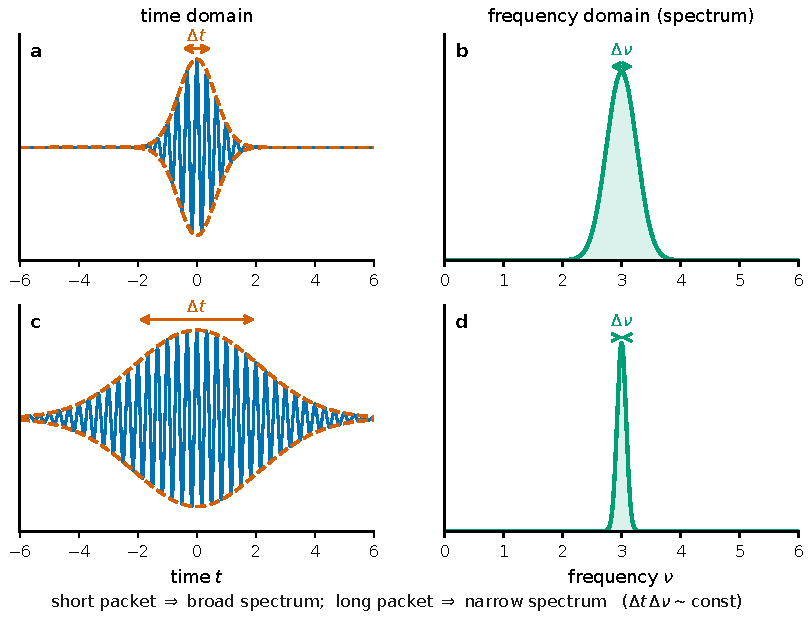
\includegraphics[width=0.9\linewidth]{figures/generated/edu_ch02/e02_wave_packet_spectrum.pdf}
\caption{The ``time--frequency reciprocity'' of finite-length wave packets. The top row is a short wave packet: pinched very narrow in time (\(\Delta t\) small, orange double arrow), yet its spectrum spreads very wide (\(\Delta\nu\) large); the bottom row is a long wave packet: stretched very long in time, its spectrum instead squeezed into a narrow peak. The orange dashed line is the envelope, the green is the corresponding spectrum. The product \(\Delta t\,\Delta\nu\) of both rows is about the same constant: this is precisely the picture of Eq.~\eqref{eq:e02-bandwidth-time}.}
\label{fig:e02-wave-packet}
\end{figure}

\section{Computing the Bandwidth as a Real Number}
\label{sec:e02-bandwidth}

In astronomical observation we usually do not know the frequency bandwidth \(\Delta\nu\) directly, but rather the filter's central wavelength \(\lambda\) and wavelength bandwidth \(\Delta\lambda\) (for example, ``500 nanometres centre, 1 nanometre half-width''). To translate it into a frequency bandwidth, we need only differentiate the relation between \(\nu\) and \(\lambda\) once. Frequency and wavelength are linked by the speed of light:
\[
  \nu=\frac{c}{\lambda}.
\]
Here \(c\approx3\times10^{10}\,{\rm cm\,s^{-1}}\) is the speed of light; following the book's CGS convention throughout, the wavelength \(\lambda\) is measured in centimetres and the frequency \(\nu\) in hertz. Differentiating with respect to \(\lambda\) (this step cannot be skipped), using \(\dfrac{d}{d\lambda}\bigl(c\lambda^{-1}\bigr)=-c\lambda^{-2}\):
\[
  \frac{d\nu}{d\lambda}=-\frac{c}{\lambda^{2}}.
\]
The negative sign indicates that frequency decreases as wavelength increases, which is the expected inverse relation; what we care about is the magnitude of the bandwidth, so we take the absolute value and replace the differential \(d\lambda\) with a finite small bandwidth \(\Delta\lambda\) (as long as \(\Delta\lambda\ll\lambda\), approximating the finite difference by the differential is accurate enough):
\begin{equation}
  \Delta\nu\;\simeq\;\frac{c\,\Delta\lambda}{\lambda^{2}} .
  \label{eq:e02-bandwidth-conversion}
\end{equation}
\begin{formulaexplain}
\(\Delta\nu\) is the frequency bandwidth, \(\Delta\lambda\) is the wavelength bandwidth, \(\lambda\) is the central wavelength, and \(c\) is the speed of light. For the same \(\Delta\lambda\), the shorter the wavelength (the smaller \(\lambda^2\)), the larger the frequency bandwidth converted.
\end{formulaexplain}
Note that the denominator is \(\lambda^{2}\) rather than \(\lambda\): this reminds us that the same ``1 nanometre'' wavelength window corresponds to a larger frequency bandwidth at the blue end than at the red end. Now let us put in real numbers. Take a visible-light filter, \(\lambda=500\,{\rm nm}=5\times10^{-5}\,{\rm cm}\), \(\Delta\lambda=1\,{\rm nm}=1\times10^{-7}\,{\rm cm}\):
\[
  \Delta\nu\simeq
  \frac{(3\times10^{10}\,{\rm cm\,s^{-1}})\times(1\times10^{-7}\,{\rm cm})}
       {(5\times10^{-5}\,{\rm cm})^{2}}
  =\frac{3\times10^{3}}{2.5\times10^{-9}}\,{\rm Hz}
  =1.2\times10^{12}\,{\rm Hz}.
\]
That is, about \(1.2\,{\rm THz}\) (terahertz). Please fix this order of magnitude firmly in mind: a 1-nanometre filter that looks ``very narrow'' in fact passes a window a trillion-plus hertz wide in frequency. Compared with the carrier frequency \(\nu_0\sim6\times10^{14}\,{\rm Hz}\), this window occupies only \(0.2\%\), and in the spectroscopic sense is indeed ``narrow''; but once converted to a timescale, it will bring about an astonishing shortness. This is precisely the protagonist of the next section.

\section{Coherence Time: How Long the Wave Remembers Its Own Phase}
\label{sec:e02-coherence-time}

Now let us translate the bandwidth of the previous section into time. Return to the iron law \eqref{eq:e02-bandwidth-time}: a stretch of light whose frequency spreads out \(\Delta\nu\) can at most keep ``coordinated'' in time for about \(\Delta t\sim1/\Delta\nu\). Let us give this time a name, the \textbf{coherence time} \(\tau_c\):
\begin{equation}
  \tau_c\;\simeq\;\frac{1}{\Delta\nu}
  \;\simeq\;\frac{\lambda^{2}}{c\,\Delta\lambda} .
  \label{eq:e02-coherence-time}
\end{equation}
\begin{formulaexplain}
\(\tau_c\) is the coherence time, in seconds; the wider the bandwidth \(\Delta\nu\), the shorter the coherence time. The second equality is just Eq.~\eqref{eq:e02-bandwidth-conversion} substituted in, expressing it in wavelength terms. It is the length of time light ``remembers its own phase,'' not the time resolution of the detector.
\end{formulaexplain}
How should we understand \(\tau_c\)? Think of light as that rotating complex-amplitude arrow. If the light were ideally single-frequency, the arrow would turn uniformly at constant angular velocity, and by glancing at where it points this instant you could accurately predict where it will point a microsecond later, or an hour later: it ``remembers its phase forever.'' But real light has bandwidth: it mixes in a whole crowd of arrows with slightly different frequencies, turning at slightly different rates; at first orderly, they spread apart as they turn, and the phase of the resultant arrow becomes ever less predictable. \(\tau_c\) is the time needed ``to go from orderly to scattered'': past \(\tau_c\), the light has basically forgotten its phase from \(\tau_c\) ago. The wider the bandwidth, the greater the spread of rates mixed in, and the faster it forgets.

Substituting the number from the previous section, \(\Delta\nu\simeq1.2\times10^{12}\,{\rm Hz}\):
\[
  \tau_c\simeq\frac{1}{1.2\times10^{12}\,{\rm Hz}}
  \approx8.3\times10^{-13}\,{\rm s}
  \approx0.8\,{\rm ps}.
\]
Less than one picosecond (\(1\,{\rm ps}=10^{-12}\,{\rm s}\)). This is the coherence time given by that ``very narrow'' 1-nanometre filter: the light can remember its own phase for only about 0.8 picoseconds, then it turns the page.

The reason this number took a whole chapter to prepare is that there is a jaw-dropping gulf between it and the capability of the detector. The fastest single-photon detectors (avalanche photodiode APD, photomultiplier tube PMT) have a time response of roughly 100 picoseconds to 1 nanosecond. Comparing with the coherence time:
\[
  \frac{\Delta t_{\rm det}}{\tau_c}\sim
  \frac{100\,{\rm ps}\;\text{to}\;1\,{\rm ns}}{0.8\,{\rm ps}}
  \approx1.2\times10^{2}\;\text{to}\;1.2\times10^{3}.
\]
That is, the width of one time gate (time bin) of the detector is \emph{hundreds to thousands of times} the coherence time. In other words, every time you record the intensity of one time gate, you are in fact averaging together hundreds or thousands of mutually incoherent, independent wave trains. The detector has no time to see clearly the phase fluctuation of any single wave train; what it sees is always the average energy after hundreds or thousands of coherence times have been smoothed out. This conclusion (``one time gate averages \(N\sim10^{2}\)--\(10^{3}\) coherence times'') will recur again and again later when we discuss photon statistics, bunching, and intensity interferometry, and directly determines by how many times the signal we can measure is diluted.

\begin{figure}[tbp]
\centering
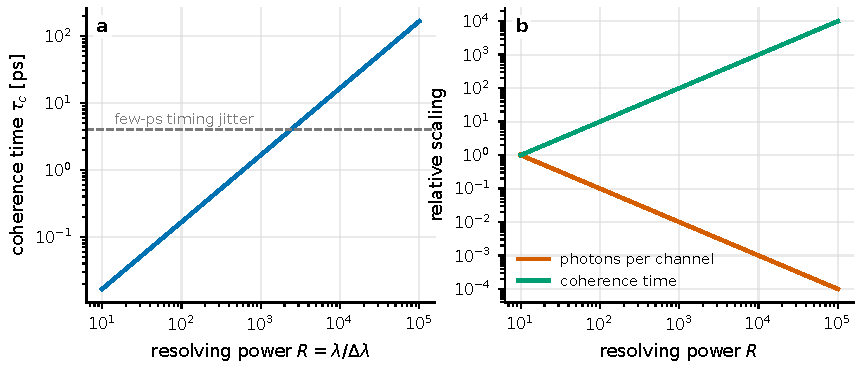
\includegraphics[width=0.85\linewidth]{figures/generated/chapter_06/ch06_spectral_resolution_coherence.pdf}
\caption{Spectral resolution and coherence time are two faces of the same thing. The narrower the spectral line (bandwidth \(\Delta\nu\)), the longer the corresponding coherence time \(\tau_c\simeq1/\Delta\nu\); conversely broadband light has an extremely short coherence time. The figure places the ps-scale \(\tau_c\) given by a visible-light broadband filter alongside the detector's 100\,ps--1\,ns response, showing that one time gate contains a great many mutually incoherent wave trains.}
\label{fig:e02-spectral-coherence}
\end{figure}

A one-sentence summary: bandwidth and coherence time are two faces of the same coin, \(\tau_c\simeq1/\Delta\nu\). Under visible-light broadband, \(\tau_c\) is as short as a picosecond, while the detector is as slow as more than a hundred picoseconds, the two differing by more than a hundredfold: this gulf is the backdrop for all the intensity measurements that follow.

\section{Autocorrelation and Power Spectrum: Toward the Coherence Function}
\label{sec:e02-autocorrelation}

Earlier we described the coherence time as ``\(\tau_c\) is the length of the phase memory,'' which is a qualitative statement. How do we quantify ``memory'' into a computable, measurable curve? The answer is the \textbf{autocorrelation function}. Its idea is extremely plain: multiply the signal by ``itself delayed by \(\tau\),'' then average, and see how alike they still are. For a (stationary) signal \(f(t)\), define
\begin{equation}
  \Gamma(\tau)=\bigl\langle f^{*}(t)\,f(t+\tau)\bigr\rangle
  =\lim_{T\to\infty}\frac{1}{T}\int_{0}^{T} f^{*}(t)\,f(t+\tau)\,dt ,
  \label{eq:e02-autocorrelation}
\end{equation}
\begin{formulaexplain}
\(\Gamma(\tau)\) is the autocorrelation function; \(\tau\) is the time delay; the angle brackets (or time integral) denote the time average; \(f^*\) is the complex conjugate. It measures the similarity between ``the signal now'' and ``the signal after \(\tau\).''
\end{formulaexplain}
When the delay \(\tau=0\), \(\Gamma(0)=\langle|f|^{2}\rangle\) is the average intensity of the signal (a positive real number, the maximum value). As \(\tau\) increases, if the signal still ``remembers'' itself, the phases of \(f^*(t)\) and \(f(t+\tau)\) remain in step, the product does not cancel after averaging, and \(\Gamma\) stays large; once \(\tau\) exceeds the coherence time, the two phases have long gone their separate ways, randomly distributed, the positive and negative products cancel in the average, and \(\Gamma\to0\). So \emph{the width over which the autocorrelation function decays from its peak to zero is precisely the coherence time \(\tau_c\)}. This turns the vague ``memory length'' of the previous section into the width of a curve, computable and measurable. The left panel of Figure~\ref{fig:e02-coherence} shows exactly this decay: the wider the bandwidth, the faster the normalized autocorrelation drops and the shorter the coherence time; the right panel draws the scaling \(\tau_c\simeq1/\Delta\nu\) as a straight line.

\begin{figure}[tbp]
\centering
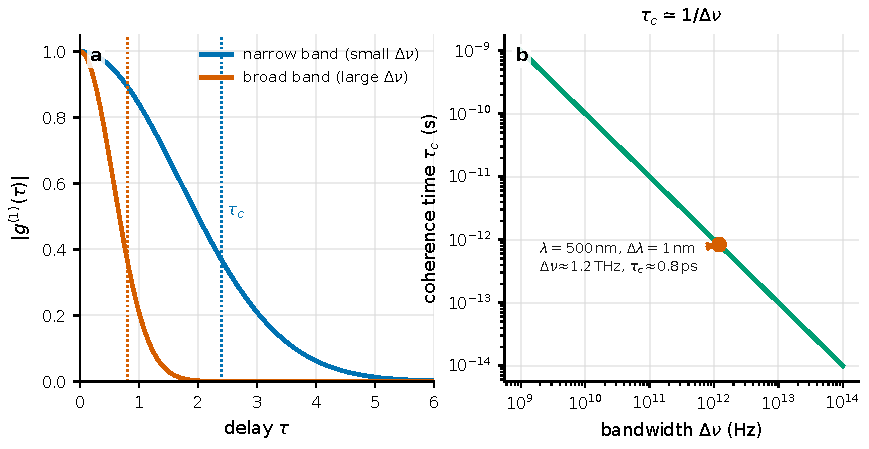
\includegraphics[width=0.92\linewidth]{figures/generated/edu_ch02/e02_coherence_bandwidth.pdf}
\caption{Coherence time and bandwidth are reciprocals of each other. Left: the normalized autocorrelation (which is also the first-order coherence \(|g^{(1)}(\tau)|\) to be formally defined later) decays with the delay \(\tau\); the wider the bandwidth (orange), the faster it drops and the shorter the coherence time \(\tau_c\), while the narrower the bandwidth (blue) the longer it ``remembers.'' Right: \(\tau_c\simeq1/\Delta\nu\) is a straight line in log-log coordinates, with the orange dot marking the \(\Delta\nu\approx1.2\,{\rm THz}\), \(\tau_c\approx0.8\,{\rm ps}\) given by the \(500\,{\rm nm}\), \(1\,{\rm nm}\) filter.}
\label{fig:e02-coherence}
\end{figure}

Finally we point out a beautiful and profound theorem that ties the chapter's two main threads (spectrum and coherence) into a single knot. This is the \textbf{Wiener--Khinchin theorem}: the \textbf{power spectrum} \(S(\nu)\) of a signal is exactly the Fourier transform of its autocorrelation function:
\begin{equation}
  S(\nu)=\int_{-\infty}^{+\infty}\Gamma(\tau)\,e^{-\,i\,2\pi\nu\tau}\,d\tau .
  \label{eq:e02-wiener-khinchin}
\end{equation}
\begin{formulaexplain}
\(S(\nu)\) is the power spectrum, telling you how much power each frequency carries; \(\Gamma(\tau)\) is the autocorrelation function. The two are a Fourier-transform pair. ``Which frequencies the signal contains'' and ``how long the signal remembers itself'' are two ways of saying the same thing.
\end{formulaexplain}
The meaning of this theorem is worth savouring slowly. It says: \emph{you need not actually measure the spectrum; just measure the autocorrelation function, take one Fourier transform, and you get the power spectrum; and vice versa}. This is exactly the rigorous embodiment of Eq.~\eqref{eq:e02-bandwidth-time}: the width of the autocorrelation (the coherence time \(\tau_c\)) and the width of the power spectrum (the bandwidth \(\Delta\nu\)) are a Fourier pair, one narrow means the other must be broad, with a product of about 1. Looking back at the Gaussian wave packet section: the time Gaussian and the frequency Gaussian are Fourier transforms of each other with inversely proportional widths, which is precisely one concrete sample of the Wiener--Khinchin theorem.

Why, in an astronomy book, do we introduce the autocorrelation so solemnly? Because the structure of that \(\langle f^*(t)f(t+\tau)\rangle\) in Eq.~\eqref{eq:e02-autocorrelation} is, almost unchanged, exactly the \textbf{first-order coherence function} \(g^{(1)}(\tau)\) to be defined later: just replace \(f\) with the electric field and normalize. That is, the autocorrelation function of this chapter is the ``classical rehearsal'' of the coherence function. When we formally introduce \(g^{(1)}\) and \(g^{(2)}\) after Chapter~\ref{chap:e05}, you will find they are not mysterious at all: \(g^{(1)}\) measures the autocorrelation of the electric field (phase memory), and its width is the \(\tau_c\) here; and between the spectral-line shape of a star and it, the bridge is precisely the Wiener--Khinchin theorem. The language this chapter has built (spectrum, bandwidth, coherence time, autocorrelation) is the foundation of the whole theory of coherence.

\section{Chapter Summary}
\label{sec:e02-summary}

\begin{itemize}
  \item \textbf{The Fourier idea}: any wave is a superposition of pure tones. A periodic signal gives discrete harmonics (Fourier series), a non-periodic signal gives a continuous spectrum (Fourier transform, Eq.~\eqref{eq:e02-fourier-transform}). The spectrum is the list of ``how much weight each frequency carries.''
  \item \textbf{Time--frequency reciprocity}: the shorter the wave train, the broader the frequency, \(\Delta\nu\,\Delta t\gtrsim1\) (Eq.~\eqref{eq:e02-bandwidth-time}). The Gaussian wave packet attains the most compact lower bound \(\sigma_t\sigma_\nu=1/2\pi\), and its Fourier transform is still a Gaussian.
  \item \textbf{Bandwidth conversion}: differentiating \(\nu=c/\lambda\) gives \(\Delta\nu\simeq c\,\Delta\lambda/\lambda^{2}\). A 500\,nm, 1\,nm filter gives \(\Delta\nu\approx1.2\times10^{12}\,{\rm Hz}\).
  \item \textbf{Coherence time}: \(\tau_c\simeq1/\Delta\nu\approx0.8\,{\rm ps}\). It is the length of time light remembers its own phase. The detector's 100\,ps--1\,ns response is a hundred to a thousand times longer: one time gate averages hundreds to thousands of coherence times.
  \item \textbf{Autocorrelation and power spectrum}: the decay width of the autocorrelation \(\Gamma(\tau)\) is the \(\tau_c\); the Wiener--Khinchin theorem (Eq.~\eqref{eq:e02-wiener-khinchin}) says the power spectrum is the Fourier transform of the autocorrelation. This is precisely the forerunner of the first-order coherence function \(g^{(1)}\).
\end{itemize}

\noindent\textbf{Questions to Ponder}:
\begin{enumerate}
  \item If the filter is changed to a \(10\,{\rm nm}\) bandwidth, what does the coherence time become? And how many coherence times are averaged in one \(1\,{\rm ns}\) time gate of the detector?
  \item A wave train interrupted by collisions on average once every \(\tau_c\), roughly how wide is its spectral line? (Hint: work backward from Eq.~\eqref{eq:e02-bandwidth-time}.)
  \item Why is ``measuring the autocorrelation function'' equivalent in information to ``measuring the spectrum''? What role does the Wiener--Khinchin theorem play in this?
\end{enumerate}

\chapter{Probability, the Poisson Process, and Shot Noise}
\label{chap:e03}

\begin{chapteropening}
In the guided-tour chapter (\ref{chap:e00}) we already saw that what a telescope ultimately hands us is not a smooth electromagnetic wave but a string of discrete clicks: at some instant, in some pixel, on some channel, ``pop,'' one photon is recorded. In the previous chapter (\ref{chap:e02}) we then learned to characterize the ``wave'' side of this light with bandwidth and coherence time; but these waves are ultimately counted out one grain at a time by the detector. Since they are ``counted'' out, there must be fluctuation: the same star, the same telescope, and you count for ten milliseconds in a row, and the number of photons counted in each millisecond is almost never the same. This is not the instrument being broken, but the breathing that ``counting'' itself carries.

This chapter sets out to explain the ``language of counting'' thoroughly in one go. We first spend a few paragraphs reviewing the smallest set of words from probability theory (random variable, expectation, variance, independence), and then, starting from the extremely plain picture of ``slicing a stretch of time into many little cells,'' derive the Poisson distribution without skipping a step, and from it obtain the golden formula that runs through the whole book: the mean equals the variance, and the noise is proportional to $\sqrt{\mu}$. Finally we ask a deeper question: if one day you measure a variance that does not equal the mean, what does that mean? This ``what does it mean'' is precisely the entrance to the entire story that the later chapters devoted to second-order coherence $g^{(2)}$ will unfold.
\end{chapteropening}

\section{The Minimal Probability Review}
\label{sec:e03-review}

Before we start counting photons, we need four words. You have met them all in general physics and probability courses; here we nail them down with just ``a paragraph plus a formula'' each, so they can be called upon directly later.

\paragraph{Random variable.}
A random variable is simply ``one experiment will give a number, but you do not know in advance which number.'' The number of photons $N$ arriving in one millisecond is the most typical random variable: it can only take non-negative integers $0,1,2,\dots$, and each value corresponds to a probability. To describe a (discrete) random variable is to give the probability $P(N)$ of it taking each value, satisfying
\begin{equation}
  P(N)\ge 0,\qquad \sum_{N=0}^{\infty}P(N)=1 .
  \label{eq:e03-normalization}
\end{equation}
\begin{formulaexplain}
$N$ is the integer count obtained in one measurement; $P(N)$ is the probability that ``this time exactly $N$ are counted.'' The first equation says probabilities are non-negative, the second says that adding up the probabilities of all possible cases must equal $1$: something has to happen.
\end{formulaexplain}
Here $N$ is a dimensionless integer (just ``how many''), and $P(N)$ is also a dimensionless pure number, taking values between $0$ and $1$. The second condition of Eq.~\eqref{eq:e03-normalization} is called normalization, and it is the ``conservation law'' that all later derivations must satisfy self-consistently: no matter how complicated a form we write the distribution in, summing $N$ from $0$ to infinity, the answer must return to $1$.

\paragraph{Expectation.}
The expectation is the ``mean value,'' but it is a theoretical, weighted mean: multiply each possible value $N$ by its probability and sum. We use angle brackets $\langle\cdot\rangle$ to denote taking the expectation,
\begin{equation}
  \langle N\rangle=\sum_{N=0}^{\infty}N\,P(N).
  \label{eq:e03-expectation}
\end{equation}
\begin{formulaexplain}
$\langle N\rangle$ is read as ``the expectation of $N$'' or ``the mean of $N$''; it weights each possible count $N$ by its probability of occurrence $P(N)$ and sums. It is not the result of any one measurement, but the average destination after infinitely many repetitions.
\end{formulaexplain}
Note that $\langle N\rangle$ is generally not an integer: an average of $100.3$ photons per millisecond is perfectly reasonable, even though any single time you can only count an integer. The expectation is additive: for any two random variables $X,Y$, $\langle X+Y\rangle=\langle X\rangle+\langle Y\rangle$, whether or not they are independent. This property that ``the expectation is always additive'' will be used repeatedly later when assembling the little cells.

\paragraph{Variance.}
Having only the mean is not enough; we also want to know ``how far each result is from the mean.'' The variance measures precisely the size of the fluctuation: take the deviation $N-\langle N\rangle$, square it (so that positive and negative deviations both become positive contributions), then take the expectation,
\begin{equation}
  \operatorname{Var}(N)=\big\langle (N-\langle N\rangle)^2\big\rangle
  =\langle N^2\rangle-\langle N\rangle^2 .
  \label{eq:e03-variance}
\end{equation}
\begin{formulaexplain}
$\operatorname{Var}(N)$ is the variance, measuring the spread of the counts about their mean; it equals ``the mean of the square'' minus ``the square of the mean.'' The larger it is, the more each counted result ``drifts.''
\end{formulaexplain}
The second equality of Eq.~\eqref{eq:e03-variance} is an identity, obtained by expanding the definition: $\langle(N-\langle N\rangle)^2\rangle=\langle N^2-2N\langle N\rangle+\langle N\rangle^2\rangle=\langle N^2\rangle-2\langle N\rangle\langle N\rangle+\langle N\rangle^2=\langle N^2\rangle-\langle N\rangle^2$, using here that the expectation is additive and that ``the expectation of a constant is itself.'' The dimension of the variance is the square of the dimension of $N$ (here $N$ is dimensionless, so the variance is dimensionless too). Its square root
\[
  \sigma=\sqrt{\operatorname{Var}(N)}
\]
is called the standard deviation, with the same unit as $N$, and is what we everyday call ``how long the error bar is.'' Remember this intuition: $\sigma$ is the ``fluctuation scale'' comparable to $N$, and the variance is its square.

\paragraph{Independence.}
Two random variables being independent means, intuitively, ``knowing the result of one is of no help whatsoever to the probability distribution of the other.'' In formula terms, the joint probability factors into the product of the individual probabilities: $P(X=x,\,Y=y)=P(X=x)\,P(Y=y)$. Independence gives us an extremely useful gift, the variance is additive:
\begin{equation}
  \operatorname{Var}(X+Y)=\operatorname{Var}(X)+\operatorname{Var}(Y)
  \quad(\text{when }X,Y\text{ are independent}).
  \label{eq:e03-var-additive}
\end{equation}
\begin{formulaexplain}
Only when $X$ and $Y$ are mutually independent does the variance of their sum equal the sum of their individual variances. This ``independent implies additive variance'' is the key lever later for assembling many little cells into one big bin and thereby computing the shot noise.
\end{formulaexplain}
Compare: the additivity of the expectation $\langle X+Y\rangle=\langle X\rangle+\langle Y\rangle$ is unconditional, whereas the additivity of the variance \eqref{eq:e03-var-additive} requires independence as a premise. The reason hides in the cross term: $\operatorname{Var}(X+Y)=\operatorname{Var}(X)+\operatorname{Var}(Y)+2\operatorname{Cov}(X,Y)$, where the covariance $\operatorname{Cov}(X,Y)=\langle XY\rangle-\langle X\rangle\langle Y\rangle$ measures the correlation of the two; when independent, $\langle XY\rangle=\langle X\rangle\langle Y\rangle$, the covariance goes to zero, and only then do the variances add cleanly. Please remember this sentence well, because the whole suspense of ``what does it mean when the variance does not equal the mean'' at the chapter's end hides in whether this covariance is zero.

With these four words in hand, we can begin to really count photons.

\section{The Mean Count in One Time Bin}
\label{sec:e03-mean}

Back in front of the telescope. In the previous chapter, the detector turned light into a string of discrete clicks. Now we do the plainest thing: choose a time window (time bin) of width denoted $\Delta t$, then count how many photons fall into this window.

If the mean photon arrival rate of this light is $R_\gamma$, then the mean count in one bin is the rate times the time:
\begin{equation}
  \mu=R_\gamma\,\Delta t .
  \label{eq:e03-mean-count}
\end{equation}
\begin{formulaexplain}
$\mu$ is the mean number of photons in one time bin (i.e.\ $\langle N\rangle$); $R_\gamma$ is the mean arrival rate, in units of $\mathrm{s^{-1}}$; $\Delta t$ is the bin width, in units of $\mathrm{s}$. Multiplying the two, the seconds cancel, and $\mu$ is the dimensionless ``how many on average.''
\end{formulaexplain}
Let us make the units and orders of magnitude concrete. The dimension of $R_\gamma$ is ``how many per second,'' i.e.\ $\mathrm{s^{-1}}$; the dimension of $\Delta t$ is the second $\mathrm{s}$; multiplying the two, the second and the ``per second'' cancel, and $\mu$ is a pure number. Take a real set of optical observation numbers: a star of moderate brightness, a metre-class telescope, a narrow-band channel, with a detected photon rate of about $R_\gamma=10^{5}\,\mathrm{s^{-1}}$; if we slice time into bins of $\Delta t=1\,\mathrm{ms}=10^{-3}\,\mathrm{s}$, then
\[
  \mu=R_\gamma\,\Delta t=10^{5}\,\mathrm{s^{-1}}\times10^{-3}\,\mathrm{s}=100 .
\]
That is, on average about $100$ photons fall in per millisecond.

Here the two words ``on average'' must be broken down and chewed through, because they are the fulcrum of everything in this chapter. Equation~\eqref{eq:e03-mean-count} absolutely does not say ``every $1\,\mathrm{ms}$ window receives exactly $100$ photons.'' It says: if you take, under completely identical conditions (the star equally bright, the telescope equally large, the efficiency equally high), thousands upon thousands of $1\,\mathrm{ms}$ windows, add up the photons counted in each window, and divide by the number of windows, this ``measured mean'' will approach $100$. In the real event stream, this one bin might be $92$, the next $107$, the next $100$: they breathe up and down around $100$. $\mu$ is the centre line of this breathing, not the measured value of any single time.

The crux is: even if you freeze all external conditions, holding the star, atmosphere, telescope, and detector perfectly still, this breathing does not go away. This is not ``uncertain instrumental noise'' but the statistical fluctuation that the very act of ``counting discrete things'' carries. To understand what law this fluctuation obeys and how large it is, we need to equip the physical intuition ``photons arrive sparsely and independently of one another'' with a set of mathematics, and that is the Poisson distribution.

\section{From the Binomial to the Poisson Distribution: A Derivation Skipping No Step}
\label{sec:e03-poisson}

\paragraph{Slicing the bin into many little cells}

The question we want to answer is: given that the mean value is $\mu$, what exactly does the probability $P(N)$ of ``counting exactly $N$'' look like?

First set up a physical assumption, the soul of the entire Poisson picture: given the mean rate, photons arrive independently and without memory of one another. By ``without memory'' we mean that the previous photon having just arrived neither summons the next one to hurry along too (that would be bunching) nor warns the next one to stay away (that would be antibunching); whether a photon appears in each extremely short stretch of time is determined only by the length of that stretch, and has nothing to do with what happened elsewhere. This is the simplest arrival pattern behind the ``on average'' of the previous section. This chapter first assumes it holds and computes the conclusion to the end; as for when it is broken, we leave that for the final section to point out.

With this assumption, we can compute using a very concrete picture. Slice the time bin of width $\Delta t$ uniformly into $M$ very short little cells, each of width
\[
  \delta t=\frac{\Delta t}{M}.
\]
As long as $M$ is large enough and $\delta t$ short enough, each little cell can hold at most one photon: the probability of two photons squeezing into the same extremely short cell at once is negligible. So each little cell degenerates into the simplest ``coin flip'': either a click (a photon appears) or nothing. The probability that a little cell registers a click is approximately
\begin{equation}
  p=R_\gamma\,\delta t .
  \label{eq:e03-cell-prob}
\end{equation}
\begin{formulaexplain}
$p$ is the probability of one click appearing in a single little cell; $R_\gamma$ is the arrival rate; $\delta t$ is the cell width. The higher the rate and the longer the cell, the greater the chance of catching a photon in this cell, but as long as $\delta t$ is short enough, $p$ is a very small number.
\end{formulaexplain}
$p$ is a dimensionless probability ($\mathrm{s^{-1}}\times\mathrm{s}$ cancels to a pure number). Note there is a self-consistency check here: the mean number of clicks over all little cells, added up, should be exactly the mean count of the whole bin. Indeed, $M$ little cells, each contributing $p$ on average, gives a total mean of
\[
  M\,p=M\cdot R_\gamma\frac{\Delta t}{M}=R_\gamma\,\Delta t=\mu .
\]
This $Mp=\mu$ is the only quantity we must ``nail fixed'' when taking the limit next: no matter how finely we slice the cells ($M\to\infty$, $p\to0$), the product $Mp$ always equals $\mu$.

\paragraph{First write down the binomial distribution}

Now counting photons becomes a pure combinatorics problem: what is the probability that ``among $M$ little cells, exactly $N$ cells registered a click''? Since the cells are mutually independent, each specific case of ``which $N$ cells click and the other $M-N$ do not'' has probability $p^{N}(1-p)^{M-N}$; and ``choosing which $N$ of the $M$ cells click'' has $\binom{M}{N}$ ways in total. Multiplying the number of ways by the probability of each case gives the binomial distribution:
\begin{equation}
  P_M(N)=\binom{M}{N}p^{N}(1-p)^{M-N},
  \qquad \binom{M}{N}=\frac{M!}{N!\,(M-N)!}.
  \label{eq:e03-binomial}
\end{equation}
\begin{formulaexplain}
$P_M(N)$ is the probability of exactly $N$ cells clicking after slicing the bin into $M$ little cells. $p^{N}$ is these $N$ cells all clicking, $(1-p)^{M-N}$ is the rest not clicking, and $\binom{M}{N}$ is the number of ways to ``choose which $N$ cells.'' Multiplying the three gives the result.
\end{formulaexplain}
This equation contains no approximation yet; it is an exact translation of the little-cell picture into a probability. $\binom{M}{N}$ is read ``$M$ choose $N$,'' the binomial coefficient; $N!$ ($N$ factorial) is the normalization factor of the number of permutations, responsible for dividing out the repetitions of ``the same few cells, only counted in a different order.'' What we do next is to let the cells become infinitely fine: $M\to\infty$, $p\to0$, while pressing down hard on $Mp=\mu$. We split Eq.~\eqref{eq:e03-binomial} into three pieces ($\binom{M}{N}$, $p^N$, $(1-p)^{M-N}$) and take the limit piece by piece.

\paragraph{\texorpdfstring{Step one: $\binom{M}{N}p^{N}\to \mu^{N}/N!$}{Step one: the limit of the binomial-coefficient term}}

Substitute $p=\mu/M$ (this is a rewriting of $Mp=\mu$), and first merge the binomial coefficient with $p^N$:
\[
  \binom{M}{N}p^{N}
  =\frac{M!}{N!\,(M-N)!}\left(\frac{\mu}{M}\right)^{N}
  =\frac{1}{N!}\cdot\frac{M!}{(M-N)!}\cdot\frac{\mu^{N}}{M^{N}} .
\]
The middle piece $\dfrac{M!}{(M-N)!}$ is in fact a product of $N$ consecutive descending factors:
\[
  \frac{M!}{(M-N)!}=M(M-1)(M-2)\cdots(M-N+1) .
\]
It has $N$ factors in all, each approximately equal to $M$ (because $N$ is a fixed finite integer while $M$ tends to infinity, so the differences of $M-1,M-2,\dots$ from $M$ are negligible). More precisely, divide it by $M^{N}$:
\[
  \frac{M(M-1)\cdots(M-N+1)}{M^{N}}
  =1\cdot\Big(1-\tfrac{1}{M}\Big)\Big(1-\tfrac{2}{M}\Big)\cdots\Big(1-\tfrac{N-1}{M}\Big)
  \xrightarrow[M\to\infty]{}1 .
\]
Each parenthesis tends to $1$ as $M\to\infty$, and there are only a fixed $N-1$ parentheses, so the whole product tends to $1$. So the limit of the first piece is clean and neat:
\begin{equation}
  \binom{M}{N}p^{N}
  =\frac{\mu^{N}}{N!}\cdot\frac{M(M-1)\cdots(M-N+1)}{M^{N}}
  \xrightarrow[M\to\infty]{}\frac{\mu^{N}}{N!}.
  \label{eq:e03-limit-first}
\end{equation}
\begin{formulaexplain}
After substituting $p=\mu/M$, the binomial coefficient merges with $p^N$; the $N$ descending factors in the numerator, divided by $M^N$, tend to $1$ one by one, leaving only $\mu^N/N!$. This step turns the ``combinatorial count of choosing cells'' into the familiar $\mu^N/N!$ of the Poisson formula.
\end{formulaexplain}

\paragraph{\texorpdfstring{Step two: $(1-p)^{M}\to e^{-\mu}$}{Step two: the limit of the no-click probability}}

Now handle the third piece $(1-p)^{M-N}$. Substituting $p=\mu/M$ likewise:
\[
  (1-p)^{M-N}=\Big(1-\frac{\mu}{M}\Big)^{M-N}
  =\Big(1-\frac{\mu}{M}\Big)^{M}\cdot\Big(1-\frac{\mu}{M}\Big)^{-N}.
\]
First look at the second factor $\big(1-\mu/M\big)^{-N}$: the exponent $-N$ is a fixed finite number, while the base $1-\mu/M\to 1$, so this factor tends to $1^{-N}=1$ and can be discarded. What really matters is the first factor $\big(1-\mu/M\big)^{M}$. Here we call upon a standard limit by name, the general form of the definition of the natural constant $e$:
\begin{equation}
  \lim_{M\to\infty}\Big(1-\frac{\mu}{M}\Big)^{M}=e^{-\mu}.
  \label{eq:e03-elimit}
\end{equation}
\begin{formulaexplain}
This is a known standard limit (the definition of $e$): $\big(1+x/M\big)^{M}\to e^{x}$, taking $x=-\mu$ gives $e^{-\mu}$. It condenses the joint probability of ``many little cells all not clicking'' into a single exponential factor.
\end{formulaexplain}
Why does \eqref{eq:e03-elimit} hold, rather than being an incantation? We can verify it by taking the logarithm, using the Taylor expansion of the logarithm $\ln(1+u)=u-\tfrac12u^{2}+\cdots$ (when $u$ is small):
\[
  \ln\Big(1-\frac{\mu}{M}\Big)^{M}
  =M\ln\Big(1-\frac{\mu}{M}\Big)
  =M\left(-\frac{\mu}{M}-\frac{\mu^{2}}{2M^{2}}-\cdots\right)
  =-\mu-\frac{\mu^{2}}{2M}-\cdots .
\]
As $M\to\infty$, all terms except the first, which contain $1/M$, vanish, leaving only $-\mu$; taking the exponential to restore gives $e^{-\mu}$. Physically, this $e^{-\mu}$ is precisely the condensation of the total probability that ``a great many little cells each register exactly no click'': $M$ little cells, each with no-click probability $1-p$, all not clicking is $(1-p)^{M}$, which in the limit becomes $e^{-\mu}$.

\paragraph{Putting it together: the Poisson distribution}

Multiplying the two limits \eqref{eq:e03-limit-first} and \eqref{eq:e03-elimit} (the discarded $\big(1-\mu/M\big)^{-N}\to1$ from the second piece already merged in), the binomial distribution \eqref{eq:e03-binomial} converges to the Poisson distribution:
\begin{equation}
  P(N)=\lim_{M\to\infty}P_M(N)
  =e^{-\mu}\,\frac{\mu^{N}}{N!}.
  \label{eq:e03-poisson}
\end{equation}
\begin{formulaexplain}
$P(N)$ is the probability of counting exactly $N$ photons in one bin when the mean count is $\mu$. $e^{-\mu}$ comes from ``many little cells not clicking,'' $\mu^{N}$ is the weight that the larger the mean the more it favours high counts, and $N!$ removes the repetition of the ordering of the clicks. This is the counting law of sparse independent arrival.
\end{formulaexplain}
Each part of this equation has a corresponding intuition. The exponential factor $e^{-\mu}$ is the ``background base note,'' representing the contribution of the great many empty little cells, the larger $\mu$ the lower it presses; $\mu^{N}$ is the ``the brighter the more skewed toward many'' climbing term; $N!$ is the combinatorial normalization, smoothing away the irrelevant ordering of who clicks first among the $N$ clicks. We can do a normalization self-check on the spot, using the Taylor series of the exponential function $\sum_{N=0}^{\infty}\mu^{N}/N!=e^{\mu}$ (this is the standard expansion of $e^{\mu}$):
\[
  \sum_{N=0}^{\infty}P(N)
  =e^{-\mu}\sum_{N=0}^{\infty}\frac{\mu^{N}}{N!}
  =e^{-\mu}\cdot e^{\mu}=1 .
\]
Just as Eq.~\eqref{eq:e03-normalization} requires, the total probability returns to $1$, showing that we did not lose or overcount any probability while taking the limit.

Let us also verify the expectation on the spot, to confirm that this $\mu$ is indeed the mean count (and not some coincidentally same-named letter). By definition \eqref{eq:e03-expectation},
\[
  \langle N\rangle
  =\sum_{N=0}^{\infty}N\,e^{-\mu}\frac{\mu^{N}}{N!}
  =e^{-\mu}\sum_{N=1}^{\infty}\frac{\mu^{N}}{(N-1)!}
  =e^{-\mu}\,\mu\sum_{N=1}^{\infty}\frac{\mu^{N-1}}{(N-1)!}
  =e^{-\mu}\,\mu\,e^{\mu}=\mu .
\]
The first step drops the $N=0$ term (which contributes zero) and sums from $N=1$; the second uses $N/N!=1/(N-1)!$ to cancel one factor; the third changes the variable to $k=N-1$, and that sum is again $e^{\mu}$. The result $\langle N\rangle=\mu$, complete. At this point the Poisson distribution lives up to its name: its mean count is precisely $\mu=R_\gamma\Delta t$.

One sentence worth stressing, lest the reader misunderstand the Poisson distribution as some ``mysterious randomness'': it describes absolutely not ``causeless chaos,'' but on the contrary the most orderly, most even-tempered kind of arrival: a string of sparse independent clicks with no extra memory, not summoning one another and not avoiding one another. Precisely because it is so ``standard,'' it becomes the baseline against which all deviations are measured.

\section{Shot Noise: The Variance Equals the Mean}
\label{sec:e03-shotnoise}

\paragraph{Computing the variance from the independent superposition of little cells}

Having the distribution, next we measure the fluctuation. We want to prove that the variance of the Poisson count is exactly equal to its mean. The least laborious and most physically flavoured method is still to return to the little-cell picture, using the lever ``independent implies additive variance'' prepared in the first section.

Give the $i$-th little cell an indicator variable $X_i$: if this cell clicks, $X_i=1$; if not, $X_i=0$. The total count is the sum over all little cells, $N=\sum_{i=1}^{M}X_i$. Each $X_i$ takes only $0$ or $1$, the simplest Bernoulli variable, whose mean and variance are easy to compute:
\[
  \langle X_i\rangle=1\cdot p+0\cdot(1-p)=p,\qquad
  \langle X_i^{2}\rangle=1^{2}\cdot p+0^{2}\cdot(1-p)=p ,
\]
so by the variance definition \eqref{eq:e03-variance},
\[
  \operatorname{Var}(X_i)=\langle X_i^{2}\rangle-\langle X_i\rangle^{2}=p-p^{2}=p(1-p).
\]
Now invoke the assumption: different little cells are mutually independent, so the variance is additive (Eq.~\eqref{eq:e03-var-additive}); adding up the $M$ identical little cells,
\[
  \operatorname{Var}(N)=\sum_{i=1}^{M}\operatorname{Var}(X_i)=M\,p(1-p)=Mp\,(1-p)=\mu\,(1-p).
\]
The last step used $Mp=\mu$. Now take the limit of infinitely fine cells $p=\mu/M\to0$, that $(1-p)$ tends to $1$, and what remains is precisely
\begin{equation}
  \operatorname{Var}(N)=\mu .
  \label{eq:e03-var-equals-mean}
\end{equation}
\begin{formulaexplain}
The variance of the Poisson count is exactly equal to its mean $\mu$. It comes from the superposition of ``$M$ independent little cells, each contributing a variance of $p(1-p)$,'' and in the fine-slicing limit $(1-p)\to1$, the total variance converges to $\mu$. Mean equal to variance is the fingerprint of Poisson statistics.
\end{formulaexplain}
Please appreciate how slender and powerful this $\operatorname{Var}(N)=\mu$ is: it says that for independently arriving photons, you need not measure anything extra: knowing only the mean count $\mu$, you automatically know the size of the fluctuation. Mean and variance are not two independent quantities, but are locked into the same number by the assumption of ``independent arrival.'' This also explains why it is called shot noise: like raindrops smacking a tin roof, the noise is not the roof being broken, but the raindrops themselves arriving discretely one grain at a time, the graininess naturally bringing fluctuation.

\paragraph{Relative noise, signal-to-noise ratio, and order of magnitude}

Having the variance, the standard deviation is its square root:
\begin{equation}
  \sigma=\sqrt{\operatorname{Var}(N)}=\sqrt{\mu}.
  \label{eq:e03-sigma}
\end{equation}
\begin{formulaexplain}
$\sigma$ is the standard deviation of the count, i.e.\ the length of the error bar, equal to $\sqrt{\mu}$. The absolute fluctuation grows with the mean count, but grows more slowly than the mean (only as the square root).
\end{formulaexplain}
Note that $\sigma=\sqrt{\mu}$ has the same dimension as $N$, both ``how many,'' and can be drawn directly as an error bar on the count: a bin with a mean of $100$ counts has a typical fluctuation of about $\sqrt{100}=10$ (see Figure~\ref{fig:e03-poisson}; that distribution spreading around $\mu$ and the fluctuation band of $\pm\sqrt{\mu}$ are the very look of this statistics). The absolute fluctuation does rise with brightness, but what really determines the quality of the measurement is how large it is relative to the signal itself. So we define the relative shot noise
\begin{equation}
  \frac{\sigma}{\mu}=\frac{\sqrt{\mu}}{\mu}=\frac{1}{\sqrt{\mu}} .
  \label{eq:e03-relative}
\end{equation}
\begin{formulaexplain}
The relative fluctuation equals $1/\sqrt{\mu}$: the more you count, the smaller the relative noise, but it improves only slowly as the square root. To halve the relative error, you must count four times as many photons.
\end{formulaexplain}
This $1/\sqrt{\mu}$ is the most oft-recited line in astronomical observation, and translating it into orders of magnitude is especially satisfying. Its reciprocal, $\mu$ against its own fluctuation, is precisely the signal-to-noise ratio (SNR):
\begin{equation}
  \mathrm{SNR}=\frac{\text{signal}}{\text{noise}}=\frac{\mu}{\sigma}=\frac{\mu}{\sqrt{\mu}}=\sqrt{\mu}.
  \label{eq:e03-snr}
\end{equation}
\begin{formulaexplain}
When pure shot noise dominates, the signal-to-noise ratio equals $\sqrt{\mu}$: divide the signal $\mu$ by its fluctuation $\sqrt{\mu}$. The more photons accumulated, the higher the signal-to-noise ratio, likewise growing as the square root.
\end{formulaexplain}
Let us put in real numbers to feel how ``expensive'' this square-root law is. If one stretch of integration accumulates on average $\mu=10^{4}$ photons, then the relative noise is $1/\sqrt{10^4}=1/100=1\%$ and the signal-to-noise ratio is $\sqrt{10^4}=100$, a rather beautiful measurement. Conversely, if in an extremely faint source, an extremely short bin, there is on average only $\mu=1$ photon, then the relative noise is $1/\sqrt{1}=100\%$ and the signal-to-noise ratio is only $1$: here the discrete count itself is the dominant noise, whether you count $0$ or $2$ is almost a coin flip, and any fine physical quantity is drowned in the raw fluctuation of ``whether there is a photon or not.''

This square-root law also incidentally explains the sense of ``twice the effort for half the result'' fatalism in astronomical observation: to press the relative error from $1\%$ further down to $0.5\%$, $\mu$ must rise from $10^4$ to $4\times10^4$: the integration time must quadruple to buy a halving of the error. Shot noise is the floor of all more complicated error budgets; later, no matter whether we add in background, dead time, or the source's own variation, we must first stand on this floor of $\sqrt{\mu}$ and build up from there.

\begin{figure}[tbp]
\centering
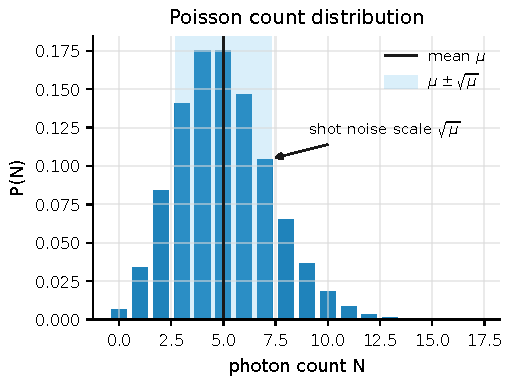
\includegraphics[width=0.85\linewidth]{figures/generated/chapter_01/ch01_photon_count_statistics.pdf}
\caption{The basic shape of the Poisson count distribution (here taking a single mean count $\mu$ as illustration). When the mean count is $\mu$, the distribution spreads around $\mu$, the variance also equals $\mu$, so the scale of the fluctuation (the error bar) is $\sqrt{\mu}$, and the relative shot noise is $1/\sqrt{\mu}$. The figure marks the mean line and the $\pm\sqrt{\mu}$ fluctuation band.}
\label{fig:e03-poisson}
\end{figure}

\section{When the Variance No Longer Equals the Mean: A Question Left for Later}
\label{sec:e03-beyond}

Now let us look at the whole chapter's logic in reverse. We obtained $\operatorname{Var}(N)=\mu$ by relying on a very hard premise: that arrivals in different little cells are mutually independent, so that the variance is additive (Eq.~\eqref{eq:e03-var-additive}). Once this premise holds, mean and variance are locked into the same number. So, conversely: if one day in an experiment you carefully measure the variance and the mean and find that they are not equal, then this chain must have broken at the link of ``independence.''

So ``whether the variance is larger or smaller than the mean'' becomes a probe reading directly the behaviour of the photons. Let us define a convenient ratio, the Mandel $Q$ parameter, to quantify the deviation:
\begin{equation}
  Q=\frac{\operatorname{Var}(N)-\mu}{\mu}.
  \label{eq:e03-mandelQ}
\end{equation}
\begin{formulaexplain}
$Q$ measures the deviation of the counting statistics from Poisson: $Q=0$ is Poisson (independent arrival); $Q>0$ the variance exceeds the mean, called super-Poisson; $Q<0$ the variance is less than the mean, called sub-Poisson. It translates ``independent or not'' into a measurable number.
\end{formulaexplain}
The three cases correspond to three utterly different physical pictures. $Q=0$, the variance equals the mean, is the Poisson baseline of this chapter, the photons not greeting one another. $Q>0$, the variance bulges out, is called super-Poissonian: the photons tend to arrive in clumps, one arrives and its companions are more likely to come in company too, as though they love to huddle: this is bunching, the hallmark of thermal light and starlight, kinds of chaotic light. $Q<0$, the variance is pressed down, is called sub-Poissonian: the photons push one another away, one has just arrived and the next deliberately hides and stays away, arriving even more ``evenly'' than random: this is antibunching, the fingerprint of genuinely non-classical light such as single-photon sources, which a classical electromagnetic wave can never produce no matter how it is manipulated.

Pushing these two pictures to the extreme, we touch the covariance planted at the chapter's end: bunching means the arrivals at neighbouring times are positively correlated ($\operatorname{Cov}>0$, the variance pushed up), and antibunching means negatively correlated ($\operatorname{Cov}<0$, the variance whittled down). Measuring this correlation strength of ``after one photon arrives, whether another photon is more or less likely to follow closely'' requires a dedicated tool: the second-order coherence function $g^{(2)}(\tau)$. What it measures is precisely the relative probability that ``given that a photon is detected at time $t$, another photon is detected again after a further $\tau$'': $g^{(2)}(0)>1$ is bunching, $g^{(2)}(0)<1$ is antibunching, and $g^{(2)}=1$ returns to the everywhere-independent Poisson baseline of this chapter.

In other words, this chapter has spoken the ``language of counting'' to its very boundary: as long as photons arrive independently, everything is locked down by the two equations $\mu=R_\gamma\Delta t$ and $\operatorname{Var}(N)=\mu$. And truly interesting astrophysics and quantum optics live precisely outside this boundary: in the place where the variance deviates from the mean, where photons begin to ``sense'' one another. How to systematically measure this deviation, and how it in turn tells us the physical nature of the source and even the angular scale of the object, is the main theme that the later chapters devoted to second-order coherence $g^{(2)}$ will unfold. By then you will see that this unassuming $\operatorname{Var}(N)=\mu$ of this chapter is the very foundation of the whole edifice of intensity interferometry.

\section{Chapter Summary}
\label{sec:e03-summary}

\begin{itemize}
  \item \textbf{Four words.} A random variable gives the probability of taking each value (normalization $\sum P(N)=1$); the expectation $\langle N\rangle$ is always additive; the variance $\operatorname{Var}(N)=\langle N^2\rangle-\langle N\rangle^2$ measures the fluctuation; independence makes the variance additive too: this is the most crucial lever of the whole chapter.
  \item \textbf{Mean count.} The mean count of one time bin is $\mu=R_\gamma\Delta t$; taking $R_\gamma=10^5\,\mathrm{s^{-1}}$, $\Delta t=1\,\mathrm{ms}$ gives $\mu=100$. ``On average'' is the destination of many same-condition bins, not the measured value of any single one.
  \item \textbf{Poisson distribution.} Slicing the bin into $M$ little cells, each with click probability $p=\mu/M$, the count follows the binomial distribution \eqref{eq:e03-binomial}; letting $M\to\infty$, using $\binom{M}{N}p^N\to\mu^N/N!$ and the standard limit $(1-\mu/M)^M\to e^{-\mu}$, gives $P(N)=e^{-\mu}\mu^N/N!$.
  \item \textbf{Shot noise.} From the independent superposition of little cells we get $\operatorname{Var}(N)=\mu$; the standard deviation $\sqrt{\mu}$, the relative shot noise $1/\sqrt{\mu}$, the signal-to-noise ratio $\sqrt{\mu}$. At $\mu=10^4$ the relative error is $1\%$; at $\mu=1$ the count itself dominates. Halving the error requires counting four times as many photons.
  \item \textbf{Beyond the boundary.} The variance deviating from the mean ($Q\neq0$) means the photons no longer arrive independently: super-Poisson corresponds to bunching, sub-Poisson to antibunching. The tool to measure this correlation is the second-order coherence function $g^{(2)}$, left for the later chapters devoted to it to unfold.
\end{itemize}

\medskip
\noindent\textbf{Questions to Ponder.}
\begin{enumerate}
  \item If the bin width $\Delta t$ is doubled, how do $\mu$, $\sigma$, and the relative noise $1/\sqrt{\mu}$ each change? And the signal-to-noise ratio?
  \item A telescope detects $10^6$ photons per second, and you want the relative shot noise of some measurement to reach $0.1\%$, at least how long must you integrate (assuming pure shot noise)?
  \item Suppose you measure a source whose variance is clearly less than the mean ($Q<0$), and after completely ruling out instrumental problems, what does this mean physically? Can a classical electromagnetic wave give such a result?
\end{enumerate}

\chapter{Quantum Mechanics and the Harmonic Oscillator: Ladder Operators}
\label{chap:e04}

\begin{chapteropening}
So far we have kept saying ``photon'' without ever seriously asking: where does a photon actually come from? It is not a little ball hidden in the vacuum ahead of time; it is a single ``step up'' of some vibrating mode. To make this statement precise, we must first return to the simplest and most important system in all of quantum mechanics: the harmonic oscillator.

This chapter has a single central question: for a system that vibrates back and forth, why can its energy take only discrete, evenly spaced values? The answer hides in two operators: one that moves you ``down one rung,'' one that moves you ``up one rung.'' They are called ladder operators. Starting from the ordinary position and momentum, we will build these two operators without skipping a single step, prove that they satisfy an exceptionally clean commutation relation, and then use them to read off the energy spectrum, the number states, and the zero-point energy all at once. This is the first cornerstone of the whole book's answer to ``where do photons come from'': once you have digested the algebra of this chapter, every later discussion of coherent states, thermal states, and photon statistics will be nothing but a generalization of it.
\end{chapteropening}

\section{A Minimal Review of Quantum Mechanics}
\label{sec:e04-review}

Before we get our hands dirty, let us lay out on the table a few quantum-mechanical ``tools'' that we will use over and over. This section proves nothing; it merely relights things you have most likely seen once before. If every item feels familiar, that is precisely the sign that you are ready.

\paragraph{State vectors.}
The state of a quantum system at a given moment is represented by a vector \(|\psi\rangle\), read ``ket psi.'' You may picture it as an arrow living in an abstract space (a Hilbert space). Its dual partner is written \(\langle\psi|\) (``bra psi''), and joining the two, \(\langle\psi|\psi\rangle\), gives the squared length of that arrow. Physically we always require a state to be normalized:
\[
  \langle\psi|\psi\rangle=1,
\]
because the total probability that ``the system is in some state'' must be 1.

\paragraph{Operators and eigenvalues.}
To every physical measurement one can make on the system (energy, position, momentum, \ldots) there corresponds an operator, which we denote with a hatted letter, for example \(\hat H,\hat x,\hat p\). An operator acting on a state produces a new state. In particular, if a state satisfies
\[
  \hat A\,|a\rangle = a\,|a\rangle,
\]
we say \(|a\rangle\) is an eigenstate of \(\hat A\), and the number \(a\) is the corresponding eigenvalue. Physically, only when the system is exactly in \(|a\rangle\) will a measurement of \(A\) yield \(a\) with certainty. Operators corresponding to observables are all Hermitian (\(\hat A^\dagger=\hat A\)), which guarantees real eigenvalues: the numbers we read out must of course be real.

\paragraph{Expectation values.}
If the state is not an eigenstate, the measurement outcome fluctuates and we can only speak of an average. Measuring \(A\) on the state \(|\psi\rangle\), the average over many repetitions is the expectation value
\begin{equation}
  \langle A\rangle \equiv \langle\psi|\,\hat A\,|\psi\rangle .
  \label{eq:e04-expectation}
\end{equation}
\begin{formulaexplain}
\(\langle A\rangle\) is the mean measured value of the observable \(A\) on the state \(|\psi\rangle\). Simply sandwich the operator \(\hat A\) between \(\langle\psi|\) and \(|\psi\rangle\). If the state is normalized, this is the average in the genuine sense.
\end{formulaexplain}
Here \(\hat A\) is the operator corresponding to the quantity to be measured, and \(|\psi\rangle\) is the current (normalized) state of the system. Equation \eqref{eq:e04-expectation} is the single ``value-extraction'' device we will use again and again in this chapter: once the state and the operator are known, any average is computed from it. It has no unit ambiguity: the units are fixed entirely by \(\hat A\), for example when \(\hat A=\hat H\), \(\langle H\rangle\) is an energy (erg).

\paragraph{Commutators.}
The order in which two operators act generally cannot be swapped, and this ``non-commutativity'' is precisely the fundamental divide between quantum and classical mechanics. We measure it with the commutator:
\begin{equation}
  [\hat A,\hat B]\equiv \hat A\hat B-\hat B\hat A .
  \label{eq:e04-commutator}
\end{equation}
\begin{formulaexplain}
\([\hat A,\hat B]\) measures the difference between ``\(B\) then \(A\)'' and ``\(A\) then \(B\).'' If it vanishes, the two quantities can be measured precisely at the same time; if it does not, they ``fight'' each other.
\end{formulaexplain}
\(\hat A\hat B\) means letting \(\hat B\) act first and then \(\hat A\) (operators act on states from right to left). If \([\hat A,\hat B]=0\), we say the two operators commute; they share common eigenstates and can have definite values simultaneously. If not, they cannot. When we later build the ladder operators, nearly every simplification step amounts to repeatedly shuffling this \(\hat A\hat B-\hat B\hat A\). One identity we will need shortly (verified by direct expansion) is
\[
  [\hat A,\hat B\hat C]=[\hat A,\hat B]\hat C+\hat B[\hat A,\hat C].
\]

\paragraph{The canonical commutation relation.}
Of all commutators, the most basic is the canonical commutation relation between position and momentum:
\begin{equation}
  [\hat x,\hat p]=i\hbar .
  \label{eq:e04-xp}
\end{equation}
\begin{formulaexplain}
\(\hat x\) is the position operator, \(\hat p\) the momentum operator, and \(\hbar\) the reduced Planck constant. They do not commute; they differ by a pure imaginary constant \(i\hbar\). This is the ``foundation brick'' of all of quantum mechanics.
\end{formulaexplain}
In \eqref{eq:e04-xp}, \(\hat x\) has the dimension of length (cm) and \(\hat p\) the dimension of momentum (\(\mathrm{g\,cm\,s^{-1}}\)); their product has the dimension of action (\(\mathrm{erg\,s}\)), consistent with \(\hbar\) (\(\hbar\simeq1.05\times10^{-27}\,\mathrm{erg\,s}\)). Note that the right-hand side is a pure number times the identity operator, independent of the state; this is exactly why it is ``fundamental.'' All the algebra in the rest of this chapter, at bottom, uses only this one relation \([\hat x,\hat p]=i\hbar\); everything else is logical deduction.

\paragraph{The uncertainty relation.}
Two non-commuting quantities cannot be determined with unlimited precision at the same time; this is the uncertainty relation. Its general form is the Robertson inequality: for any two Hermitian operators \(\hat A,\hat B\), their standard deviations in any state satisfy
\[
  \Delta A\,\Delta B\ \ge\ \frac12\big|\langle[\hat A,\hat B]\rangle\big| .
\]
The right-hand side of this inequality is set precisely by the commutator: the more two quantities ``fail to commute,'' the less they can be determined together. We will not prove it in this review; we simply take it as a known result and use it. Now set \(\hat A=\hat x,\hat B=\hat p\) and substitute the canonical commutation relation \eqref{eq:e04-xp}, \([\hat x,\hat p]=i\hbar\); the right-hand expectation value \(\langle i\hbar\rangle=i\hbar\) (a pure constant, independent of state), so \(\tfrac12|\langle[\hat x,\hat p]\rangle|=\tfrac12|i\hbar|=\hbar/2\), giving the most famous instance:
\[
  \Delta x\,\Delta p\ \ge\ \frac{\hbar}{2},
\]
where \(\Delta x=\sqrt{\langle \hat x^2\rangle-\langle\hat x\rangle^2}\) is the standard deviation of position and \(\Delta p\) is defined analogously. It tells us that a quantum state cannot simultaneously push both position and momentum down to zero fluctuation. Remember this ``minimum area \(\hbar/2\),'' because the ground state of the harmonic oscillator is exactly the state that saturates this inequality; it is the ``quietest'' vibration that quantum fluctuations allow. That ends this section; our toolkit is now complete.

\section{The Quantum Harmonic Oscillator and the Construction of Ladder Operators}
\label{sec:e04-ladder}

Now to the main event. Picture a small ball tied to a spring vibrating back and forth, or two atoms in a diatomic molecule stretching relative to each other, or (and this is what we really care about) the oscillation of a single mode of the electromagnetic field. Mathematically they are the same system: the harmonic oscillator. In quantum mechanics, its Hamiltonian (the energy operator) is
\begin{equation}
  \hat H=\frac{\hat p^2}{2m}+\frac{1}{2}m\omega^2\hat x^2 .
  \label{eq:e04-hamiltonian}
\end{equation}
\begin{formulaexplain}
The first term \(\hat p^2/2m\) is the kinetic energy, the second \(\tfrac12 m\omega^2\hat x^2\) is the spring potential energy. \(m\) is the mass and \(\omega\) the angular frequency of vibration. The whole expression is the quantum version of ``kinetic plus potential energy.''
\end{formulaexplain}
In \eqref{eq:e04-hamiltonian}, \(m\) is the mass (g), \(\omega\) the angular frequency (\(\mathrm{rad\,s^{-1}}\)), and \(\hat x,\hat p\) the position and momentum operators of the previous section. The whole thing has the dimension of energy (erg). Classically, this system oscillates sinusoidally at frequency \(\omega\), and its energy can take any positive value continuously. The quantum question is: what do the eigenvalues of \(\hat H\) (that is, the allowed energies) look like?

Solving the differential equation directly is of course possible, but it would drown us in special functions. There is a far more elegant path: factor \(\hat H\). Notice that \(\hat p^2/2m+\tfrac12 m\omega^2\hat x^2\) has the shape of \(a^2+b^2\), and \(a^2+b^2=(a-ib)(a+ib)\), except that \(\hat x\) and \(\hat p\) do not commute, so the factorization leaves behind a ``tail,'' and that tail hides all the physics. To this end we define two new operators:
\begin{equation}
  \hat a=\sqrt{\frac{m\omega}{2\hbar}}\left(\hat x+\frac{i\,\hat p}{m\omega}\right),
  \qquad
  \hat a^\dagger=\sqrt{\frac{m\omega}{2\hbar}}\left(\hat x-\frac{i\,\hat p}{m\omega}\right).
  \label{eq:e04-adef}
\end{equation}
\begin{formulaexplain}
\(\hat a\) is the annihilation operator, \(\hat a^\dagger\) the creation operator; the two are Hermitian conjugates of each other. They package the dimensionful \(\hat x,\hat p\) into a dimensionless combination and are the ``keys'' to the energy ladder.
\end{formulaexplain}
First a word on dimensions, to confirm these two definitions are ``clean.'' The coefficient \(\sqrt{m\omega/2\hbar}\) has dimension \(\sqrt{\mathrm{g}\cdot\mathrm{s^{-1}}/\mathrm{erg\,s}}=\mathrm{cm^{-1}}\) (since \(\mathrm{erg}=\mathrm{g\,cm^2\,s^{-2}}\)); multiplied by \(\hat x\) of dimension cm, it gives a pure number. Likewise \(\hat p/(m\omega)\) has dimension \(\mathrm{g\,cm\,s^{-1}}/(\mathrm{g\,s^{-1}})=\mathrm{cm}\), which also becomes a pure number. So \(\hat a,\hat a^\dagger\) are both dimensionless operators; this matters, because they count ``which rung'' and should not carry units to begin with. Since \(\hat x,\hat p\) are Hermitian, taking the Hermitian conjugate of \eqref{eq:e04-adef} (\(i\to -i\)) immediately shows that \(\hat a\) and \(\hat a^\dagger\) are indeed conjugates.

\paragraph{Solving back for \(\hat x,\hat p\).}
After defining these, we will often need to invert and express \(\hat x,\hat p\) through \(\hat a,\hat a^\dagger\). Just add and subtract the two lines of \eqref{eq:e04-adef}: adding cancels the imaginary parts, subtracting cancels the real parts,
\[
  \hat a+\hat a^\dagger=\sqrt{\frac{m\omega}{2\hbar}}\,(2\hat x),
  \qquad
  \hat a-\hat a^\dagger=\sqrt{\frac{m\omega}{2\hbar}}\,\frac{2i\,\hat p}{m\omega}.
\]
Hence
\begin{equation}
  \hat x=\sqrt{\frac{\hbar}{2m\omega}}\,(\hat a+\hat a^\dagger),
  \qquad
  \hat p=-i\sqrt{\frac{m\omega\hbar}{2}}\,(\hat a-\hat a^\dagger).
  \label{eq:e04-xp-in-a}
\end{equation}
\begin{formulaexplain}
Position and momentum rewritten as combinations of the creation and annihilation operators. \(\hat x\) corresponds to the ``symmetric'' combination \(\hat a+\hat a^\dagger\), \(\hat p\) to the ``antisymmetric'' combination \(\hat a-\hat a^\dagger\), each with a dimensionful prefactor.
\end{formulaexplain}
These two relations will be used repeatedly later: any quantity containing \(\hat x,\hat p\) (for instance the electric field, which is proportional to \(\hat x\)) can be translated into the language of creation and annihilation operators. The prefactor \(\sqrt{\hbar/2m\omega}\) has exactly the dimension cm, and \(\sqrt{m\omega\hbar/2}\) exactly the units of momentum, dimensionally self-consistent.

\paragraph{The key step: computing \([\hat a,\hat a^\dagger]\).}
This is the single most important piece of algebra in the chapter, and we do it without skipping a step. Substitute the definitions \eqref{eq:e04-adef} into the commutator, first pulling out the constant coefficient \(m\omega/2\hbar\):
\[
  [\hat a,\hat a^\dagger]
  =\frac{m\omega}{2\hbar}
  \left[\hat x+\frac{i\hat p}{m\omega},\ \hat x-\frac{i\hat p}{m\omega}\right].
\]
The commutator is linear in both slots, so expand it into four terms:
\[
  \left[\hat x+\tfrac{i\hat p}{m\omega},\ \hat x-\tfrac{i\hat p}{m\omega}\right]
  =[\hat x,\hat x]
  -\frac{i}{m\omega}[\hat x,\hat p]
  +\frac{i}{m\omega}[\hat p,\hat x]
  -\frac{i^2}{(m\omega)^2}[\hat p,\hat p].
\]
Now handle each term. Any operator commutes with itself, so \([\hat x,\hat x]=[\hat p,\hat p]=0\), and the first and fourth terms vanish outright. The middle two use the canonical commutation relation \eqref{eq:e04-xp}: \([\hat x,\hat p]=i\hbar\), and \([\hat p,\hat x]=-[\hat x,\hat p]=-i\hbar\). Substituting:
\[
  =-\frac{i}{m\omega}(i\hbar)+\frac{i}{m\omega}(-i\hbar)
  =-\frac{i^2\hbar}{m\omega}-\frac{i^2\hbar}{m\omega}
  =\frac{\hbar}{m\omega}+\frac{\hbar}{m\omega}
  =\frac{2\hbar}{m\omega},
\]
where we used \(i^2=-1\). Multiplying back by the leading coefficient:
\[
  [\hat a,\hat a^\dagger]=\frac{m\omega}{2\hbar}\cdot\frac{2\hbar}{m\omega}=1.
\]
And so we obtain the ``main theorem'' of the chapter:
\begin{equation}
  [\hat a,\hat a^\dagger]=1 .
  \label{eq:e04-aacomm}
\end{equation}
\begin{formulaexplain}
The commutator of the creation and annihilation operators equals 1. This extraordinarily simple relation is the source of the entire quantum structure of the harmonic oscillator (and of every field mode to come); the energy levels, the photons, and the zero-point energy all grow out of it.
\end{formulaexplain}
Savor how clean this equation is: the dimensionful \(\hat x,\hat p\), the dimensionful \(m,\omega,\hbar\), all cancel, leaving nothing but a bare 1. It is dimensionless and independent of which particular oscillator we have. Equation \eqref{eq:e04-aacomm} will become the only commutation relation we need to remember; from this moment on we can almost forget \(\hat x,\hat p\) and work entirely within the algebra of \(\hat a,\hat a^\dagger\). By contrast, the creation operators among themselves and the annihilation operators among themselves of course commute: \([\hat a,\hat a]=[\hat a^\dagger,\hat a^\dagger]=0\).

\section{Rewriting the Hamiltonian with the Number Operator}
\label{sec:e04-numberH}

We built \(\hat a,\hat a^\dagger\) in order to simplify \(\hat H\). Now we translate \eqref{eq:e04-hamiltonian} into the language of creation and annihilation operators. The most economical approach is to first compute the combination \(\hat a^\dagger\hat a\) and see how far it is from \(\hat H\). Using the definitions \eqref{eq:e04-adef} and pulling out the coefficient:
\[
  \hat a^\dagger\hat a
  =\frac{m\omega}{2\hbar}
  \left(\hat x-\frac{i\hat p}{m\omega}\right)\!\left(\hat x+\frac{i\hat p}{m\omega}\right).
\]
Carefully multiply out the brackets (keeping the operator order, since they do not commute):
\[
  \left(\hat x-\tfrac{i\hat p}{m\omega}\right)\!\left(\hat x+\tfrac{i\hat p}{m\omega}\right)
  =\hat x^2+\frac{i}{m\omega}\hat x\hat p-\frac{i}{m\omega}\hat p\hat x-\frac{i^2}{(m\omega)^2}\hat p^2 .
\]
Combine the middle two terms; they form exactly a commutator: \(\dfrac{i}{m\omega}(\hat x\hat p-\hat p\hat x)=\dfrac{i}{m\omega}[\hat x,\hat p]=\dfrac{i}{m\omega}(i\hbar)=-\dfrac{\hbar}{m\omega}\). And the last term \(-i^2\hat p^2/(m\omega)^2=+\hat p^2/(m\omega)^2\). Hence
\[
  \hat a^\dagger\hat a
  =\frac{m\omega}{2\hbar}
  \left(\hat x^2+\frac{\hat p^2}{(m\omega)^2}-\frac{\hbar}{m\omega}\right)
  =\frac{m\omega}{2\hbar}\hat x^2+\frac{1}{2\hbar m\omega}\hat p^2-\frac12 .
\]
Multiply each of the first two terms by \(\hbar\omega\) to check whether they are \(\hat H\):
\[
  \hbar\omega\left(\frac{m\omega}{2\hbar}\hat x^2\right)=\frac12 m\omega^2\hat x^2,
  \qquad
  \hbar\omega\left(\frac{1}{2\hbar m\omega}\hat p^2\right)=\frac{\hat p^2}{2m}.
\]
These are exactly the potential and kinetic terms of \eqref{eq:e04-hamiltonian}! So \(\hbar\omega\,\hat a^\dagger\hat a=\hat H-\tfrac12\hbar\omega\), and rearranging gives
\begin{equation}
  \hat H=\hbar\omega\left(\hat a^\dagger\hat a+\frac12\right)
        =\hbar\omega\left(\hat n+\frac12\right),
  \qquad \hat n\equiv\hat a^\dagger\hat a .
  \label{eq:e04-Hn}
\end{equation}
\begin{formulaexplain}
The Hamiltonian is written as a simple linear function of the number operator \(\hat n=\hat a^\dagger\hat a\). The energy equals ``the number of excitation rungs \(\hat n\) plus half a rung'' times \(\hbar\omega\). That half rung is the zero-point energy.
\end{formulaexplain}
Here \(\hat n=\hat a^\dagger\hat a\) is called the number operator. It is Hermitian (\((\hat a^\dagger\hat a)^\dagger=\hat a^\dagger\hat a\)) and thus has real eigenvalues; we will see shortly that its eigenvalues are exactly \(0,1,2,\ldots\), that is, ``how many quanta are in this mode.'' Equation \eqref{eq:e04-Hn} completely simplifies the problem of finding the spectrum: once we know the eigenvalues of \(\hat n\), the energy is read off. Dimensionally, \(\hat n\) is dimensionless and \(\hbar\omega\) is an energy, all consistent.

\paragraph{Zero-point energy.}
The \(+\tfrac12\) in \eqref{eq:e04-Hn} is not a dispensable constant. Even when \(\hat n\) takes its minimum value 0, the energy is not zero but
\[
  E_0=\frac12\hbar\omega .
\]
This is the zero-point energy. Physically it is a direct consequence of the uncertainty relation: if the oscillator truly sat still at the bottom of the potential well, it would have both a definite position (\(x=0\)) and a definite momentum (\(p=0\)), violating \(\Delta x\,\Delta p\ge\hbar/2\). Quantum mechanics does not permit this ``absolute quiet,'' so even in the ground state the oscillator must retain a minimal amount of jitter, corresponding to the energy \(\tfrac12\hbar\omega\). This jitter is not a shortcoming of our measuring ability but a property of the vacuum itself; when we later discuss the light field, it is precisely this ``vacuum fluctuation'' that gives the physical starting point for shot noise and squeezed states. For an order of magnitude: for a visible-light mode with \(\nu\sim6\times10^{14}\,\mathrm{Hz}\), \(\hbar\omega=h\nu\simeq(6.6\times10^{-27})(6\times10^{14})\,\mathrm{erg}\simeq4\times10^{-12}\,\mathrm{erg}\approx2.5\,\mathrm{eV}\), so the zero-point energy is about 1.2 eV, by no means negligible.

\section{Number States: Energy, One Rung at a Time}
\label{sec:e04-numberstates}

Now let us read off the spectrum. By \eqref{eq:e04-Hn}, \(\hat H\) and \(\hat n\) differ only by a constant and a positive factor, so they share eigenstates. Let the eigenstate of \(\hat n\) be \(|n\rangle\) with eigenvalue \(n\):
\[
  \hat n\,|n\rangle=n\,|n\rangle .
\]
We call \(|n\rangle\) a number state, or Fock state. For now \(n\) is only an undetermined real number; the task of this section is to use the commutation relation \eqref{eq:e04-aacomm} to force it to be a non-negative integer, and along the way to find out exactly what \(\hat a,\hat a^\dagger\) give when acting on \(|n\rangle\).

\paragraph{Why the ladder operators ``climb the stairs.''}
First compute two key commutators. Using \([\hat a,\hat a^\dagger]=1\):
\[
  [\hat n,\hat a]=[\hat a^\dagger\hat a,\hat a]
  =\hat a^\dagger[\hat a,\hat a]+[\hat a^\dagger,\hat a]\hat a
  =0+(-1)\hat a=-\hat a,
\]
where we used the expansion identity \([\hat A\hat B,\hat C]=\hat A[\hat B,\hat C]+[\hat A,\hat C]\hat B\) and \([\hat a^\dagger,\hat a]=-1\). Likewise
\[
  [\hat n,\hat a^\dagger]=\hat a^\dagger[\hat a,\hat a^\dagger]+[\hat a^\dagger,\hat a^\dagger]\hat a
  =\hat a^\dagger(1)+0=+\hat a^\dagger .
\]
These two, \([\hat n,\hat a]=-\hat a\) and \([\hat n,\hat a^\dagger]=+\hat a^\dagger\), are the mechanical principle of the ``ladder.'' See how they work: let \(\hat n\) act on the new state \(\hat a|n\rangle\),
\[
  \hat n\,(\hat a|n\rangle)
  =(\hat a\hat n+[\hat n,\hat a])|n\rangle
  =(\hat a\hat n-\hat a)|n\rangle
  =\hat a(\hat n-1)|n\rangle
  =(n-1)\,\hat a|n\rangle .
\]
Read this line: \(\hat a|n\rangle\) is again an eigenstate of \(\hat n\), with the eigenvalue lowered by 1 to \(n-1\). So \(\hat a\) takes the system ``down one rung''; this is why it is called the annihilation operator. Entirely symmetrically,
\[
  \hat n\,(\hat a^\dagger|n\rangle)=(n+1)\,\hat a^\dagger|n\rangle,
\]
so \(\hat a^\dagger\) lifts the system ``up one rung'' and is the creation operator. This is the origin of the word ``ladder.''

\paragraph{The ladder must have a floor: \(n\) is a non-negative integer.}
Why can the steps not extend downward without bound into negative numbers? Because the eigenvalues of \(\hat n\) cannot be negative. Using \eqref{eq:e04-expectation}, compute the expectation of \(\hat n\) on the normalized \(|n\rangle\):
\[
  n=\langle n|\hat n|n\rangle=\langle n|\hat a^\dagger\hat a|n\rangle
  =\big(\hat a|n\rangle\big)^\dagger\big(\hat a|n\rangle\big)
  =\big\|\,\hat a|n\rangle\,\big\|^2\ \ge 0 .
\]
The crucial step is the middle one: \(\langle n|\hat a^\dagger\hat a|n\rangle\) is the inner product of the state \(\hat a|n\rangle\) with itself, that is, its squared length, and the squared length of any vector is non-negative. So \(n\ge0\). But \(\hat a\) lowers the eigenvalue by 1 each time it acts; if we started from some non-integer \(n\) and applied \(\hat a\) repeatedly, sooner or later we would drop below 0 and obtain a negative eigenvalue, a contradiction. The only way out is that this descending chain must land exactly on 0 at some step and stop there; that is, there exists a ground state \(|0\rangle\) satisfying
\begin{equation}
  \hat a\,|0\rangle=0 .
  \label{eq:e04-ground}
\end{equation}
\begin{formulaexplain}
The annihilation operator acting on the ground state gives zero (not the state \(|0\rangle\), but the zero vector). This says ``we have already reached the very bottom; there is no step further down.'' The ground state is the floor of the entire energy ladder.
\end{formulaexplain}
Only when the descending sequence is cut off at \(n=0\) by \eqref{eq:e04-ground} can negative eigenvalues be avoided. Working backward from this: climbing up from \(|0\rangle\) one step at a time with \(\hat a^\dagger\), the eigenvalues obtained can only be \(0,1,2,3,\ldots\). In other words, the excitation number of the harmonic oscillator can only be a non-negative integer, and this is precisely the mathematical root of ``photons can only come one at a time.''

\paragraph{Normalization factors: where the two \(\sqrt{\ }\) come from.}
We know \(\hat a|n\rangle\) is proportional to \(|n-1\rangle\), but what is the proportionality constant? This step must be worked out fully, because the factors in the later photon statistics all rely on it. Let \(\hat a|n\rangle=c_n|n-1\rangle\), where \(c_n\) is an undetermined constant and \(|n-1\rangle\) is already normalized. Take the squared norm of both sides:
\[
  \big\|\hat a|n\rangle\big\|^2
  =|c_n|^2\,\langle n-1|n-1\rangle
  =|c_n|^2 .
\]
And the left side we just computed: \(\big\|\hat a|n\rangle\big\|^2=\langle n|\hat a^\dagger\hat a|n\rangle=\langle n|\hat n|n\rangle=n\). So \(|c_n|^2=n\), and taking the positive-real phase convention gives \(c_n=\sqrt{n}\). Entirely analogously, to find \(\hat a^\dagger|n\rangle=d_n|n+1\rangle\) we need the action of \(\hat a\hat a^\dagger\); by \eqref{eq:e04-aacomm}, \(\hat a\hat a^\dagger=\hat a^\dagger\hat a+1=\hat n+1\), so
\[
  \big\|\hat a^\dagger|n\rangle\big\|^2
  =\langle n|\hat a\hat a^\dagger|n\rangle
  =\langle n|(\hat n+1)|n\rangle
  =n+1
  =|d_n|^2,
\]
giving \(d_n=\sqrt{n+1}\). Writing the two conclusions side by side:
\begin{equation}
  \hat a\,|n\rangle=\sqrt{n}\,|n-1\rangle,
  \qquad
  \hat a^\dagger\,|n\rangle=\sqrt{n+1}\,|n+1\rangle .
  \label{eq:e04-ladder-action}
\end{equation}
\begin{formulaexplain}
The annihilation operator lowers \(|n\rangle\) to \(|n-1\rangle\) with coefficient \(\sqrt{n}\); the creation operator raises it to \(|n+1\rangle\) with coefficient \(\sqrt{n+1}\). These two square-root factors will appear in every photon-counting formula to come.
\end{formulaexplain}
Note two details. First, when \(n=0\), \(\sqrt{n}=0\), and the first relation degenerates automatically into \(\hat a|0\rangle=0\), consistent with \eqref{eq:e04-ground}, the floor is indeed sealed. Second, the coefficients are not simply 1 but \(\sqrt n\) and \(\sqrt{n+1}\): it is exactly this nonlinearity, ``the higher the step, the bigger the stride,'' that gives the photon statistics of coherent and thermal states their distinctive shapes. Equation \eqref{eq:e04-ladder-action} also gives the recipe for constructing any number state: build up from the ground state by repeated application of \(\hat a^\dagger\),
\[
  |n\rangle=\frac{(\hat a^\dagger)^n}{\sqrt{n!}}\,|0\rangle,
\]
where \(\sqrt{n!}\) is precisely the accumulated product \(\sqrt{1}\cdot\sqrt{2}\cdots\sqrt{n}\) picked up along the way.

\paragraph{Energy levels: an evenly spaced ladder.}
Substituting \(\hat n|n\rangle=n|n\rangle\) back into \eqref{eq:e04-Hn}, the energy eigenvalues are read off immediately:
\begin{equation}
  E_n=\hbar\omega\left(n+\frac12\right),\qquad n=0,1,2,\ldots
  \label{eq:e04-energy}
\end{equation}
\begin{formulaexplain}
The energy of the \(n\)th level. Adjacent levels are always spaced by \(\hbar\omega\), and the lowest level is not 0 but \(\tfrac12\hbar\omega\). The whole spectrum is a uniform ladder whose base is raised by half a rung.
\end{formulaexplain}
Equation \eqref{eq:e04-energy} is the accounting summary of this chapter's harvest. It has two striking features. First, the energy levels are discrete and evenly spaced: any two adjacent levels always differ by \(E_{n+1}-E_n=\hbar\omega\), no more and no less. Precisely because of this ``constant one rung,'' we can flatly say ``absorb one quantum of \(\hbar\omega\) and go up a level, emit one and go down a level'', and this one quantum, for an electromagnetic field mode, is one photon. Let us drop into real orders of magnitude to see how big this ``one rung'' is: for a typical diatomic-molecule stretching vibration \(\omega/2\pi\sim10^{13}\text{--}10^{14}\,\mathrm{Hz}\) (the infrared band), the adjacent-level spacing is \(\hbar\omega\sim0.1\text{--}0.5\,\mathrm{eV}\), exactly the energy of infrared spectral lines; while for the visible-light single mode we truly care about, \(\nu\sim6\times10^{14}\,\mathrm{Hz}\), one rung is \(\hbar\omega\approx2.5\,\mathrm{eV}\), precisely the energy of one visible photon. Same ladder; change \(\omega\) and you go from molecular vibration to the light field. Second, the base is lifted by the zero-point energy to \(\tfrac12\hbar\omega\), as described in the previous section. Draw \(E_n\) out and you get an evenly spaced ladder starting at \(\tfrac12\hbar\omega\) and rising by \(\hbar\omega\) per level; the number state \(|n\rangle\) is the state standing on the \(n\)th rung, carrying \(n\) energy quanta. At this point, the question ``where do photons come from,'' at the single-mode level, has a complete answer: a photon is one rung of excitation on the energy ladder of the harmonic oscillator; \(\hat a^\dagger\) creates it, \(\hat a\) annihilates it. Figure~\ref{fig:e04-energy-ladder} draws this entire ``ladder'' out.

\begin{figure}[tbp]
\centering
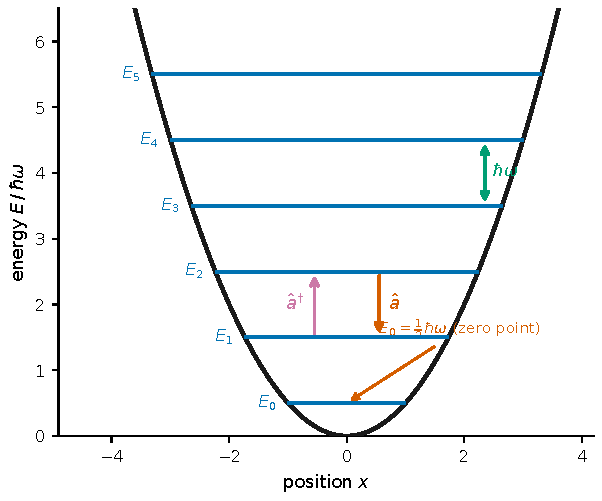
\includegraphics[width=0.6\linewidth]{figures/generated/edu_ch04/e04_energy_ladder.pdf}
\caption{The energy ladder of the quantum harmonic oscillator. In the potential well \(V(x)=\tfrac12 m\omega^2 x^2\), the allowed energies can only take the evenly spaced rungs \(E_n=\hbar\omega(n+\tfrac12)\): adjacent levels always differ by \(\hbar\omega\) (green double arrow), and the lowest level is not zero but the zero-point energy \(\tfrac12\hbar\omega\) (orange). The creation operator \(\hat a^\dagger\) lifts the system up one rung and the annihilation operator \(\hat a\) lowers it one rung. This ``constant one rung'' \(\hbar\omega\), for an electromagnetic field mode, is the energy of one photon.}
\label{fig:e04-energy-ladder}
\end{figure}

\section{A Preview: The Quantum State Closest to Classical Vibration}
\label{sec:e04-coherent}

The number state \(|n\rangle\) has the most definite energy, yet it is also the least ``like'' a classical vibration. Consider: the position of a classical oscillator traces a beautiful sinusoid over time, \(x(t)=x_0\cos\omega t\), but the position expectation of a number state \(\langle n|\hat x|n\rangle\) is identically zero, since by \eqref{eq:e04-xp-in-a}, \(\hat x\propto\hat a+\hat a^\dagger\) only turns \(|n\rangle\) into \(|n\pm1\rangle\), which is orthogonal to \(\langle n|\), giving inner product zero. That is, a quantum oscillator of definite energy has a position expectation that does not swing at all; in phase space it is a uniformly blurred ring, with no information whatsoever about ``which side it is on right now.'' This runs exactly counter to our everyday intuition about ``vibration.''

So which quantum state is the closest to classical back-and-forth swinging? The answer is the coherent state \(|\alpha\rangle\), defined as an eigenstate of the annihilation operator:
\begin{equation}
  \hat a\,|\alpha\rangle=\alpha\,|\alpha\rangle,\qquad \alpha\in\mathbb{C}.
  \label{eq:e04-coherent}
\end{equation}
\begin{formulaexplain}
The coherent state is an eigenstate of the annihilation operator \(\hat a\), with eigenvalue \(\alpha\) a complex number. The modulus of the complex number gives the mean photon number, its argument gives the vibration phase. It is the ``closest to classical'' quantum state.
\end{formulaexplain}
This definition looks strange at first: \(\hat a\) is not Hermitian, and its eigenvalue \(\alpha\) is allowed to be complex. But it is exactly this complex number that encodes amplitude and phase for us at once: \(|\alpha|\) sets how strong the vibration is (one can show the mean photon number \(\langle\hat n\rangle=|\alpha|^2\)), and \(\arg\alpha\) sets which phase it has swung to right now. One can show that the position expectation of a coherent state does indeed oscillate sinusoidally in time, and that it pushes the joint fluctuation of position and momentum down to the minimum allowed by the uncertainty relation; it is a small ``spot'' of light of constant size, translating uniformly around a circle in time, looking just like a classical point carrying a quantum blur.

Let us picture the two states on the same phase-space map (horizontal axis position \(x\), vertical axis momentum \(p\)). The image of the number state \(|n\rangle\) is a whole ring of uniform blur: its energy (the square of the radius) is definite, but the expectations of both position and momentum are identically zero and the phase is entirely undetermined, and you cannot say ``which point on the circle it has swung to right now,'' because it is smeared over the entire ring at once. The image of the coherent state \(|\alpha\rangle\), on the other hand, is a small, compact spot pinned to one point on the circle: it has a definite center, whose distance from the origin is about \(|\alpha|\) and whose azimuth is the phase \(\arg\alpha\), and this spot revolves uniformly around the circle in time, exactly reproducing the classical sinusoidal vibration \(x(t)\propto\cos\omega t\). Remember the difference of the two in one sentence: the number state is a ``ring smeared out into a full circle,'' the coherent state is a ``spot condensed to a point, translating around the circle.'' Figure~\ref{fig:e04-phase-space} draws these two phase-space pictures side by side.

\begin{figure}[tbp]
\centering
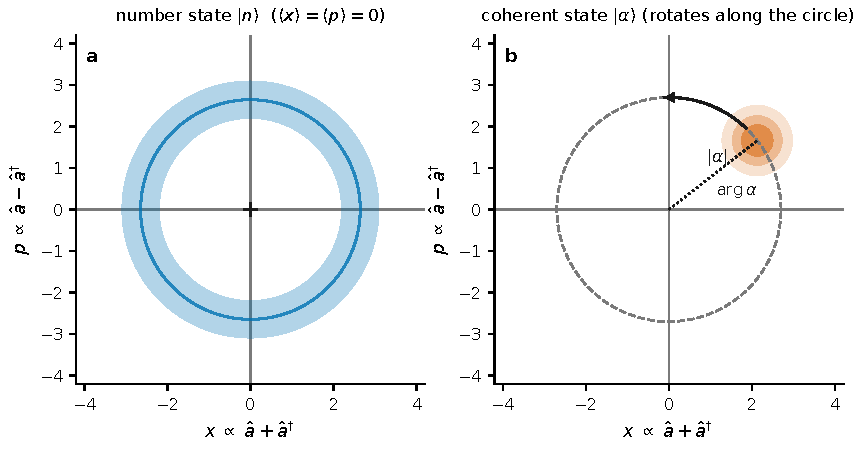
\includegraphics[width=0.92\linewidth]{figures/generated/edu_ch04/e04_phase_space_states.pdf}
\caption{Two extreme quantum states in phase space (horizontal axis \(x\propto\hat a+\hat a^\dagger\), vertical axis \(p\propto\hat a-\hat a^\dagger\)). Left: the number state \(|n\rangle\) has definite energy (the square of the ring radius is fixed) but spreads its probability uniformly over a full circle, with zero expectation of both position and momentum and completely undetermined phase, like a blurred ring. Right: the coherent state \(|\alpha\rangle\) condenses into a small, compact spot pinned to the circle of radius about \(|\alpha|\) and azimuth \(\arg\alpha\), revolving uniformly around the circle and reproducing the classical sinusoidal vibration.}
\label{fig:e04-phase-space}
\end{figure}

Here we merely set out the definition \eqref{eq:e04-coherent} and give an intuition; the detailed development (that its photon number follows a Poisson distribution, how it is written as a superposition of number states, why it is the natural starting point for lasers and stellar thermal light) is left to Chapter~\ref{chap:e06}. You need only remember one sentence: the number state is the extreme of ``most definite energy, most blurred phase,'' and the coherent state is the opposite extreme of ``clearest phase, most like classical swinging,'' and both use the same \(\hat a,\hat a^\dagger\).

\section{Chapter Summary}
\label{sec:e04-summary}

\begin{itemize}
  \item The entire quantum structure of the harmonic oscillator requires only one canonical commutation relation \([\hat x,\hat p]=i\hbar\). From it we define \(\hat a,\hat a^\dagger\) (Eq.~\eqref{eq:e04-adef}), and a term-by-term computation gives the core relation \([\hat a,\hat a^\dagger]=1\) (Eq.~\eqref{eq:e04-aacomm}); thereafter we can work entirely within the algebra of \(\hat a,\hat a^\dagger\).
  \item The Hamiltonian is rewritten as \(\hat H=\hbar\omega(\hat n+\tfrac12)\), where the number operator is \(\hat n=\hat a^\dagger\hat a\). That \(+\tfrac12\) is the zero-point energy \(\tfrac12\hbar\omega\), a direct consequence of the uncertainty relation forbidding the oscillator to be absolutely still.
  \item Using \([\hat n,\hat a]=-\hat a\) and \([\hat n,\hat a^\dagger]=+\hat a^\dagger\) we prove that \(\hat a,\hat a^\dagger\) lower/raise the eigenvalue rung by rung; using \(\langle n|\hat a^\dagger\hat a|n\rangle=n\ge0\) we force the eigenvalue to be a non-negative integer, with the ladder sealed at the floor by \(\hat a|0\rangle=0\).
  \item Normalization gives \(\hat a|n\rangle=\sqrt{n}\,|n-1\rangle\) and \(\hat a^\dagger|n\rangle=\sqrt{n+1}\,|n+1\rangle\), and the spectrum is an evenly spaced ladder \(E_n=\hbar\omega(n+\tfrac12)\). The adjacent-level spacing \(\hbar\omega\) is the energy of ``one photon.''
  \item The number state is the state of most definite energy and most blurred phase; the coherent state \(|\alpha\rangle\) (\(\hat a|\alpha\rangle=\alpha|\alpha\rangle\)) is the closest to classical vibration; see Chapter~\ref{chap:e06}.
\end{itemize}

\paragraph{Questions to Ponder.}
\begin{itemize}
  \item If you replaced \([\hat x,\hat p]=i\hbar\) by the classical \([\hat x,\hat p]=0\) and redid the derivation, what would \([\hat a,\hat a^\dagger]\) become? Would the energy levels still be discrete? This reveals to whom, exactly, the discrete levels are owed.
  \item The number state \(|n\rangle\) has position expectation \(\langle\hat x\rangle=0\), yet \(\langle\hat x^2\rangle\) grows with \(n\). Using \eqref{eq:e04-xp-in-a} and \eqref{eq:e04-ladder-action}, compute \(\langle n|\hat x^2|n\rangle\) and see whether it is proportional to \((n+\tfrac12)\), and explain the connection between this result and the zero-point energy.
  \item Why does ``absorbing one quantum of \(\hbar\omega\)'' mean ``one more photon'' for the electromagnetic field? Connect the energy ladder of the harmonic oscillator to the photon number and explain it in your own words.
\end{itemize}

\chapter{Quantizing Light: From Modes to Photons}
\label{chap:e05}

\begin{chapteropening}
In the previous chapter we quantized a single isolated harmonic oscillator: the energy can only be taken in discrete portions, the annihilation operator \(\hat a\) removes one portion, the creation operator \(\hat a^\dagger\) adds one. But that was only a ``spring.'' What a real telescope faces is an electromagnetic field that fills all of space, has color, has direction, has polarization, and fluctuates in time. What this chapter sets out to do is to replicate the success of that single harmonic oscillator of Chapter~\ref{chap:e04} onto the entire light field (tens of thousands of times over), and the method takes only one step: first decompose the light field into a set of ``modes,'' and then, to our surprise, discover that every mode is mathematically just a harmonic oscillator. At this point the word ``photon'' obtains a precise definition for the first time: it is not a little ball, but a single excitation of some mode. By the end of this chapter you will understand exactly what each ``click'' recorded by a telescope belongs to, and you will also compute one counterintuitive fact: as bright as the Sun is, each optical mode holds, on average, less than one hundredth of a photon.
\end{chapteropening}

\section{Why Decompose the Light Field into ``Modes''}
\label{sec:e05-why-modes}

Let us begin with a plain question: the electromagnetic field is a continuous thing pervading all of space, and what a telescope receives at any instant is a big blob of oscillating field. How are we to ``count it in discrete portions''?

The key to the answer is to not fixate from the outset on a continuous quantity like ``the field strength at a certain point at a certain time,'' but instead to switch to a smarter set of coordinates. Recall the Fourier analysis of Chapter~\ref{chap:e02}: any complicated stretch of sound wave can be written uniquely as a superposition of a bunch of ``pure tones'' (sinusoids of a single frequency). Pure tones are the simplest, mutually independent ``building blocks'' of the world of sound. \textbf{A mode is the electromagnetic-field version of a ``generalized pure tone.''}

A mode of the electromagnetic field is a ``building block'' labeled simultaneously by the following several things:

\begin{itemize}
  \item \textbf{Frequency}\(\ \omega\) (or color \(\nu=\omega/2\pi\)): how fast this block oscillates;
  \item \textbf{Spatial shape}\ \(u(\bm r)\): what this block looks like in space: a plane wave propagating in some direction, a diffraction-limited spot, or a guided mode in an optical fiber;
  \item \textbf{Polarization}: which way the electric-field vector points in the plane perpendicular to propagation: horizontal, vertical, or some rotation;
  \item \textbf{Time window}\ \(\Delta t\): the stretch of time this block is ``switched on.''
\end{itemize}

The reason we go to the trouble of choosing such a set of building blocks is that we want them to be \emph{mutually orthogonal, not interfering with one another}. Orthogonal here means exactly the same as ``pure tones of different frequencies are mutually independent'' in Fourier analysis: expand the field along this set of modes, and the coefficient of each mode can be measured separately, evolves separately, and is quantized separately, without any entanglement between them. Mathematically, a set of mode functions \(\{u_k(\bm r)\}\) satisfies orthonormality
\[
  \int u_i^*(\bm r)\,u_j(\bm r)\,\mathrm d^3r=\delta_{ij},
\]
where \(\delta_{ij}\) is the Kronecker delta (1 when \(i=j\), otherwise 0). With such a set of ``generalized pure tones,'' Maxwell's equations allow us to write the entire electromagnetic field as
\[
  \bm E(\bm r,t)=\sum_k\big[\,(\text{amplitude of the }k\text{th mode})\times u_k(\bm r)\,e^{-i\omega_k t}+\text{complex conjugate}\,\big].
\]
Each term oscillates independently at its own frequency \(\omega_k\); this is exactly what a ``generalized pure tone'' should look like. In the next section we fix our gaze on any one of these \(k\) and see what equation of motion its amplitude obeys.

\section{The Key Step: Every Mode Is a Harmonic Oscillator}
\label{sec:e05-mode-is-oscillator}

Now lock attention onto a single mode \(k\). Its spatial shape \(u_k(\bm r)\) is fixed; the only thing still in motion is its amplitude, call it \(q_k(t)\). What we will do is substitute this single-mode field into the energy density of the electromagnetic field, integrate over space, and see what the total energy it carries looks like. This step, in standard electrodynamics, is called the ``mode expansion of the field energy''; many textbooks (such as the section on cavity modes in Jackson's \emph{Classical Electrodynamics}, or the first chapter of any introductory quantum-optics book) do it. But it is precisely the \emph{foundation} of this chapter, and skipping over it would leave the self-taught reader unable to prove it for themselves, so we walk through this piece of algebra exactly as it is. Only three facts are really needed, and we call each of them by name as we go.

\textbf{Fact one: the electromagnetic energy-density formula.} The total energy of a free electromagnetic field enclosed in a volume is (in CGS units)
\[
  U=\frac{1}{8\pi}\int\big(\bm E^2+\bm B^2\big)\,\mathrm d^3r,
\]
the electric-field term and the magnetic-field term contributing symmetrically half each; this is a result you learned back in general-physics electromagnetism, in units of erg.

\textbf{Fact two: how to write the single-mode field.} Keep only the \(k\)th mode in the expression. Taking it to be a real standing wave (a cavity mode), the electric field can be written as ``spatial shape \(\times\) time-varying amplitude'':
\[
  \bm E_k(\bm r,t)=-\,c_1\,\dot q_k(t)\,\bm u_k(\bm r),
\]
where \(\bm u_k\) is the orthonormal mode function of the previous section, \(q_k(t)\) is the amplitude coordinate we are tracking, and \(c_1\) is a proportionality factor containing only constants (\(4\pi\), \(c\), etc.); we carry it along for now, and it will in the end be absorbed into the definition of \(q_k\).

\textbf{Fact three: Maxwell's equations tie \(\dot{\bm E}\) and \(\bm B\) together.} In vacuum \(\nabla\times\bm B=\tfrac1c\,\partial_t\bm E\), so the magnetic field is determined by the time derivative of the electric field. Substituting \(\bm E_k\propto\dot q_k\,\bm u_k\) of fact two, the right side \(\propto\ddot q_k\,\bm u_k\); for a mode oscillating harmonically at \(\omega_k\), \(\ddot q_k=-\omega_k^2 q_k\), so the time part of the magnetic field is proportional to \(q_k(t)\) itself, while the spatial part is determined by \(\nabla\times\bm u_k\):
\[
  \bm B_k(\bm r,t)=c_2\,q_k(t)\,\big[\nabla\times\bm u_k(\bm r)\big].
\]
Here the mode also satisfies the Helmholtz equation \(\nabla^2\bm u_k=-(\omega_k^2/c^2)\,\bm u_k\) (``the degree of curvature of the spatial shape sets the frequency''), which will presently help us compute the spatial integral of the magnetic-field term into a number containing \(\omega_k^2\).

Now substitute facts two and three into the integral of fact one. The electric-field term gives
\[
  \frac1{8\pi}\int\bm E_k^2\,\mathrm d^3r
  =\frac{c_1^2}{8\pi}\,\dot q_k^{\,2}\int|\bm u_k|^2\,\mathrm d^3r
  =\frac{c_1^2}{8\pi}\,\dot q_k^{\,2},
\]
where the last step used precisely the \emph{orthonormality} \(\int|\bm u_k|^2\,\mathrm d^3r=1\) of the previous section, at once turning the spatial integral into 1. Likewise, doing the same integral in the magnetic-field term (using \(\int|\nabla\times\bm u_k|^2\,\mathrm d^3r=(\omega_k^2/c^2)\int|\bm u_k|^2\,\mathrm d^3r=\omega_k^2/c^2\), a step that uses the Helmholtz equation) gives
\[
  \frac1{8\pi}\int\bm B_k^2\,\mathrm d^3r
  =\frac{c_2^2}{8\pi}\,q_k^{\,2}\cdot\frac{\omega_k^2}{c^2}
  \ \propto\ \omega_k^2\,q_k^{\,2}.
\]
So the electric-field term \(\propto\dot q_k^{\,2}\) and the magnetic-field term \(\propto\omega_k^2 q_k^{\,2}\); putting the two together, the energy takes on the ``kinetic plus potential'' form of a harmonic oscillator:
\[
  U_k=(\text{constant}_1)\,\dot q_k^{\,2}+(\text{constant}_2)\,\omega_k^2\,q_k^{\,2}.
\]
The last step is the crucial one: those two constants (both assembled from \(c_1,c_2,4\pi,c\), etc.) are \emph{not} irrelevant. We \textbf{redefine \(q_k\)} so that it absorbs these constants together (physically this can always be done: it is just multiplying the amplitude by a constant factor). Choosing this normalization is defining \(q_k\) to be the \emph{canonical coordinate} of this mode, with the effective mass taken to be 1. Then both coefficients become exactly \(\tfrac12\), and the energy equals exactly
\[
  H_k=\tfrac12\,\dot q_k^{\,2}+\tfrac12\,\omega_k^2\,q_k^{\,2}.
\]
Read this line three times. It is \emph{identical} to the energy of that mass-1 spring of Chapter~\ref{chap:e04}, \(H=\tfrac12\dot q^2+\tfrac12\omega^2 q^2\); note that this is an exact \emph{equality}, not ``proportional to'': that once-ambiguous proportionality constant has already been swallowed by our definition of \(q_k\), so the effective mass is exactly 1 and not some other coefficient. In other words:

\begin{quote}
\textbf{Every electromagnetic field mode is, mathematically, a harmonic oscillator of frequency \(\omega_k\).}
\end{quote}

This is the pivot of the whole chapter. Once we grant this sentence, we \emph{need invent nothing new}; we simply apply, word for word, the quantization we did for the harmonic oscillator in Chapter~\ref{chap:e04} to each mode. In Chapter~\ref{chap:e04} we packaged \(q,\dot q\) into an annihilation operator \(\hat a\) and a creation operator \(\hat a^\dagger\). Here we do the same for the \(k\)th mode, obtaining a pair \(\hat a_k,\hat a_k^\dagger\). Because different modes are mutually orthogonal and do not interfere, their operator commutation relations are

\begin{equation}
  [\hat a_i,\hat a_j^\dagger]=\delta_{ij},\qquad
  [\hat a_i,\hat a_j]=0,\qquad
  \hat n_k=\hat a_k^\dagger\hat a_k .
  \label{eq:e05-commutator}
\end{equation}
\begin{formulaexplain}
\(\hat a_k^\dagger,\hat a_k\) add and remove one photon in the \(k\)th mode; \(\delta_{ij}\) says that only the creation and annihilation of the \emph{same} mode leave a quantum correction behind, and different modes are completely independent; \(\hat n_k\) counts how many photons are in the \(k\)th mode.
\end{formulaexplain}

Let us account for each symbol. \(\hat a_k\) is the annihilation operator of the \(k\)th mode, dimensionless; it lowers the excitation number of that mode by one. \(\hat a_k^\dagger\) is the creation operator, which raises the excitation number by one. The physical meaning of the commutator \(\delta_{ij}\) is one of the key points of this chapter: when \(i\neq j\), \([\hat a_i,\hat a_j^\dagger]=0\), meaning ``photons in the red-light mode'' and ``photons in the blue-light mode'' are two utterly unrelated ledgers that can be counted separately; this is exactly the reward for our having chosen \emph{orthogonal} modes in the first place. The eigenvalues of the number operator \(\hat n_k=\hat a_k^\dagger\hat a_k\) are \(N_k=0,1,2,\dots\), pure integers with no units, and it counts ``how many portions of excitation are in the \(k\)th mode right now.''

One portion of excitation is one photon. At this point, ``photon'' finally has an unambiguous definition: a photon is not a bullet flying through space, but \emph{the energy of one definite mode (a definite frequency, a definite spatial shape, a definite polarization) raised by one whole portion}. The same photon necessarily belongs to some mode; asking ``where is this photon'' is equivalent to asking ``which mode does it belong to.''

\section{The Positive-Frequency Field Operator: Photons Make Their Formal Entrance}
\label{sec:e05-field-operator}

Reassembling the annihilation operators of each mode from the previous section according to spatial shape and frequency yields the quantized electric field. What a detector truly uses when it ``absorbs a photon'' is the half of the electric field containing only \(\hat a_k\) (annihilation), called the \textbf{positive-frequency field operator}:

\begin{equation}
  \hat E^{(+)}(\bm r,t)=\sum_k \mathcal E_k\,u_k(\bm r)\,e^{-i\omega_k t}\,\hat a_k .
  \label{eq:e05-field-expansion}
\end{equation}
\begin{formulaexplain}
The light field written as a sum over a bunch of modes: in the \(k\)th term, \(\mathcal E_k\) is the normalization coefficient for ``how strong one photon is,'' \(u_k(\bm r)\) is the spatial shape of the mode, \(e^{-i\omega_k t}\) is its oscillation, and \(\hat a_k\) \emph{removes one photon} from this mode. The whole expression is ``the light the detector sees.''
\end{formulaexplain}

Let us make each symbol clear; this equation is the foundation of all the later chapters.

\begin{itemize}
  \item \(\hat E^{(+)}(\bm r,t)\): the positive-frequency electric-field operator, containing the ``annihilation'' part. \(\bm r\) is position (units cm), \(t\) is time (units s).
  \item \(\mathcal E_k\): the single-photon field strength, that is, the normalization factor for ``how big an electric field one photon in this mode corresponds to.'' It converts the dimensionless operator \(\hat a_k\) into a genuine field strength (in CGS, units \(\mathrm{statvolt\,cm^{-1}}\)). It is set by the mode's frequency and effective volume; by order of magnitude \(\mathcal E_k\propto\sqrt{\hbar\omega_k/V}\); here \(V\) is the effective volume of the mode (units cm\(^3\)), \(\hbar=h/2\pi\) is the reduced Planck constant (\(h\) the Planck constant, see Section~\ref{sec:e05-occupation}), and the numerator \(\hbar\omega_k=h\nu_k\) is exactly the energy of one photon. The higher the frequency and the smaller the mode volume, the stronger the field of a single photon.
  \item \(u_k(\bm r)\): the spatial mode function of the \(k\)th mode, dimensionless (already orthonormalized per the previous section), carrying ``what this block looks like and which way it goes.''
  \item \(e^{-i\omega_k t}\): the time oscillation of this mode, \(\omega_k=2\pi\nu_k\) being the angular frequency (units \(\mathrm{rad\,s^{-1}}\)). The sign convention makes it the ``positive-frequency'' part.
  \item \(\hat a_k\): the annihilation operator. It is the only ``quantum'' ingredient in this equation; because of it, the electric field is no longer a number but an operator that can change the photon number.
\end{itemize}

Where did the other half (the part containing only the creation operator \(\hat a_k^\dagger\)) go? It is the Hermitian conjugate of \eqref{eq:e05-field-expansion}:
\[
  \hat E^{(-)}(\bm r,t)=\big[\hat E^{(+)}(\bm r,t)\big]^\dagger
  =\sum_k \mathcal E_k^*\,u_k^*(\bm r)\,e^{+i\omega_k t}\,\hat a_k^\dagger .
\]
Adding the two halves, \(\hat{\bm E}=\hat E^{(+)}+\hat E^{(-)}\), is the complete, observable (Hermitian) electric-field operator. Why split them apart? Because \textbf{photodetection is essentially absorption}: an electron in the detector is ``knocked'' out by light by \emph{taking away} one photon from the light field, and this process uses only the annihilation operator \(\hat a_k\), that is, only \(\hat E^{(+)}\). And so we obtain a sentence that runs through the whole book:

\begin{quote}
\textbf{Detecting one photon is decreasing the photon number in some mode by one}; mathematically it is \(\hat E^{(+)}\) (containing \(\hat a_k\)) acting on the light state.
\end{quote}

A telescope never reads out \(\hat a_k\) or \(\hat E\) directly; what it reads out are time stamps, pixels, energy channels, polarization channels, all of which are products of \(\hat n_k\), or of correlations of several \(\hat n\), after passing through the instrument response. But conceptually, behind every click stands an \(\hat a_k\): some mode, one photon fewer.

\section{Number States of Light: Fock States}
\label{sec:e05-fock}

Since every mode is a harmonic oscillator, the energy eigenstates of the harmonic oscillator naturally upgrade into the energy eigenstates of the light field. The state in which the \(k\)th mode has exactly \(N_k\) photons is written \(|N_k\rangle\), satisfying \(\hat n_k|N_k\rangle=N_k|N_k\rangle\). Specifying the occupation numbers of all modes together yields a \textbf{number state} of the entire light field, also called a \textbf{Fock state}:

\begin{equation}
  |\{N_k\}\rangle=|N_1,N_2,N_3,\dots\rangle,
  \qquad
  \hat n_k\,|\{N_k\}\rangle=N_k\,|\{N_k\}\rangle .
  \label{eq:e05-fock}
\end{equation}
\begin{formulaexplain}
A Fock state is a ``roll call'': \(N_1\) photons in mode 1, \(N_2\) photons in mode 2, \ldots; every number is definite, with no fluctuation. It is the exact answer-state to the question ``exactly how many photons are in each mode.''
\end{formulaexplain}

Here \(N_k=0,1,2,\dots\) is the photon number of the \(k\)th mode, a pure integer with no units. The physical meaning of a number state is very clean: it \emph{pins down the photon number of every mode}, with no fluctuation whatsoever. For example, \(|0,0,\dots\rangle\) (all modes empty) is the electromagnetic vacuum; \(|0,1,0,\dots\rangle\) is the single-photon state of ``only one photon in mode 2, all others empty.'' Any Fock state can be built up with creation operators, just as in Chapter~\ref{chap:e04} we climbed the energy ladder rung by rung with \(\hat a^\dagger\):
\[
  |\{N_k\}\rangle=\prod_k\frac{(\hat a_k^\dagger)^{N_k}}{\sqrt{N_k!}}\,|0\rangle,
\]
where \(\sqrt{N_k!}\) is the normalization factor (its origin identical to the single-mode case of Chapter~\ref{chap:e04}, normalized once for each mode here). Fock states are the ``coordinate basis'' for understanding all states of light: the coherent states and thermal states to come will both be written as superpositions or mixtures of Fock states. And the most important lesson they teach is: the information carried by light hides in the \emph{photon number} and the \emph{correlations of photon number}, not in a continuous waveform.

\section{Exactly How Many Modes Are in One Channel}
\label{sec:e05-mode-count}

Here is the pitfall most easily stepped into in astronomical observation: in a data file, ``one channel'' (one pixel, one time bin, one filter) is almost \emph{never} a single quantum mode, but a sum of very many modes. To get the physics right, we must first learn to count: how many independent modes are packed into one observing channel?

The idea is ``multiply the resolvable cells in phase space.'' The three kinds of mode labels (time, space, polarization) are mutually independent, so the total mode count is the product of each one's cell count. Let us count term by term.

\paragraph{Time modes.} A wave packet of bandwidth \(\Delta\nu\) has a time over which it ``remembers its own phase'' (the coherence time) of about \(\tau_c\simeq1/\Delta\nu\) (this is exactly the Fourier conclusion of Chapter~\ref{chap:e02}, ``shorter in time, wider in spectrum''). So an observing time window of length \(\Delta t\) holds about
\[
  \frac{\Delta t}{\tau_c}
\]
mutually independent time modes; every \(\tau_c\), the field ``forgets'' its previous phase, equivalent to switching to a fresh building block.

\paragraph{Spatial modes.} Diffraction determines how large an ``\'etendue'' (area \(\times\) solid angle) one spatial mode occupies. A beam of diffraction-limited single-mode light has an area-solid-angle product of about \(A\Omega\sim\lambda^2\) (another way of writing the diffraction limit \(\Delta\theta\sim\lambda/D\)). If the telescope together with the back end receives an \'etendue \(A\Omega\), then the number of spatial modes it holds is about
\[
  \frac{A\Omega}{\lambda^2}.
\]
A diffraction-limited imaging of a point source gives \(A\Omega\sim\lambda^2\), that is, a single spatial mode; whereas an image smeared out by atmospheric jitter (seeing), or coupled into a thick fiber, or falling on a large pixel, takes in many spatial modes at once.

\paragraph{Polarization modes.} The electric field has two independent polarization directions perpendicular to propagation. If the observation does not project the polarization onto a single channel, then multiply again by the polarization mode count \(N_{\rm pol}\) (usually 1 or 2).

Multiplying the three terms gives the effective mode count:

\begin{equation}
  M\simeq
  \underbrace{\frac{\Delta t}{\tau_c}}_{\text{time}}\,
  \underbrace{\frac{A\Omega}{\lambda^2}}_{\text{space}}\,
  \underbrace{N_{\rm pol}}_{\text{polarization}},
  \qquad
  \tau_c\simeq\frac1{\Delta\nu}\simeq\frac{\lambda^2}{c\,\Delta\lambda}.
  \label{eq:e05-mode-number}
\end{equation}
\begin{formulaexplain}
Effective mode count = number of time cells \(\times\) number of spatial cells \(\times\) number of polarizations. It tells you that an observing channel is really the average of \(M\) quantum modes; the larger \(M\) is, the more fiercely the quantum fluctuations are diluted.
\end{formulaexplain}

Where does that last \(\tau_c\simeq\lambda^2/(c\,\Delta\lambda)\) come from? Differentiating \(\nu=c/\lambda\), \(|\mathrm d\nu|=(c/\lambda^2)\,|\mathrm d\lambda|\), that is, the bandwidth conversion \(\Delta\nu\simeq c\,\Delta\lambda/\lambda^2\) (consistent with the notation of Chapter~\ref{chap:e02}); taking the reciprocal gives \(\tau_c\simeq\lambda^2/(c\,\Delta\lambda)\).

Let us plug in real numbers to get a feel. Take visible light \(\lambda=500\,\mathrm{nm}=5\times10^{-5}\,\mathrm{cm}\), filter bandwidth \(\Delta\lambda=1\,\mathrm{nm}=10^{-7}\,\mathrm{cm}\), and \(c=3\times10^{10}\,\mathrm{cm\,s^{-1}}\):
\[
  \Delta\nu\simeq\frac{c\,\Delta\lambda}{\lambda^2}
  =\frac{(3\times10^{10})(10^{-7})}{(5\times10^{-5})^2}\,\mathrm{Hz}
  \simeq1.2\times10^{12}\,\mathrm{Hz},
  \qquad
  \tau_c\simeq\frac1{\Delta\nu}\simeq0.8\,\mathrm{ps}.
\]
The coherence time is less than 1 picosecond! Yet even the fastest photodetectors have a time response on the order of \(100\,\mathrm{ps}\sim1\,\mathrm{ns}\). This means that even with a detector that ``runs blazingly fast,'' one time bin has already packed in \(\Delta t/\tau_c\sim10^2\)--\(10^3\) independent time modes. Adding on the spatial modes smeared by seeing, an astronomical channel readily becomes a sum of \emph{thousands upon thousands of modes}. Remember this sentence; it will later explain why the bunching and non-classical signals of astronomical light are always ``diluted'' so shallowly:

\begin{quote}
\textbf{``One channel'' in astronomy is usually not a single quantum mode, but a sum of many modes.}
\end{quote}

\section{Single-Mode Boson Occupation: Every Mode Is Actually Quite Dim}
\label{sec:e05-occupation}

One last order of magnitude will thoroughly change your intuition about ``how bright a star is.'' The question is: for the continuum light of a star, on average \emph{how many photons are in each mode}?

Treat a mode of some frequency \(\nu\) as a harmonic oscillator in equilibrium with a heat bath at brightness temperature \(T_b\). When this mode has \(N\) photons the energy is \(N h\nu\) (the energy ladder of Chapter~\ref{chap:e04}, taking the part above the zero-point energy here). In thermal equilibrium the probability of \(N\) photons appearing is given by the Boltzmann weight, proportional to \(e^{-Nh\nu/k_{\rm B}T_b}\). For notational convenience, write
\[
  x\equiv e^{-h\nu/k_{\rm B}T_b}\quad(0<x<1),\qquad
  P(N)=\frac{x^N}{\sum_{M=0}^{\infty}x^M}.
\]
The denominator is a geometric series, and using the summation formula for common ratio \(x\), \(\sum_{M=0}^{\infty}x^M=1/(1-x)\) (convergent since \(0<x<1\)), the normalized probability is the geometric distribution
\[
  P(N)=(1-x)\,x^N .
\]
Now compute the mean occupation \(\bar n_\nu=\langle N\rangle=\sum_{N=0}^{\infty}N\,P(N)\). The key is that step involving the sum with \(N\). Use a standard trick: differentiate the geometric series term by term,
\[
  \sum_{N=0}^{\infty}N\,x^N
  =x\,\frac{\mathrm d}{\mathrm dx}\sum_{N=0}^{\infty}x^N
  =x\,\frac{\mathrm d}{\mathrm dx}\!\left(\frac1{1-x}\right)
  =\frac{x}{(1-x)^2}.
\]
Substituting back, that \((1-x)\) cancels exactly once:
\[
  \bar n_\nu=(1-x)\sum_{N=0}^{\infty}N\,x^N
  =(1-x)\cdot\frac{x}{(1-x)^2}
  =\frac{x}{1-x}
  =\frac1{\,1/x-1\,}.
\]
Substituting \(1/x=e^{+h\nu/k_{\rm B}T_b}\) back in gives the closing formula of this chapter, the single-mode boson occupation, the familiar factor in the Planck distribution:

\begin{equation}
  \bar n_\nu=\frac1{\exp(h\nu/k_{\rm B}T_b)-1}.
  \label{eq:e05-occupation}
\end{equation}
\begin{formulaexplain}
\(\bar n_\nu\) is ``how many photons are in each mode on average.'' \(h\nu\) is the energy of one photon, \(k_{\rm B}T_b\) is the thermal energy corresponding to the brightness temperature; the larger the ratio of the two, the exponentially smaller the occupation. It measures ``how many photons per mode,'' not ``how many photons in total.''
\end{formulaexplain}

Let us account for each unit. Both \(h\nu\) and \(k_{\rm B}T_b\) are energies (units erg in CGS): \(h\) is the Planck constant, \(k_{\rm B}\) the Boltzmann constant, and \(T_b\) the brightness temperature (units K). \(\bar n_\nu\) is dimensionless, simply a pure ``mean photon number.''

Substitute the Sun. Take a stellar surface brightness temperature \(T_b=5800\,\mathrm{K}\) and wavelength \(\lambda=500\,\mathrm{nm}\). The photon energy is \(h\nu=hc/\lambda\). Using the convenient value \(hc\simeq1240\,\mathrm{eV\,nm}\), we get \(h\nu\simeq1240/500\simeq2.48\,\mathrm{eV}\); the thermal energy \(k_{\rm B}T_b\simeq(8.62\times10^{-5}\,\mathrm{eV\,K^{-1}})(5800\,\mathrm{K})\simeq0.50\,\mathrm{eV}\). So the ratio that decides everything is
\[
  \frac{h\nu}{k_{\rm B}T_b}\simeq\frac{2.48}{0.50}\simeq5.0 .
\]
Substituting into \eqref{eq:e05-occupation}:
\[
  \bar n_\nu\simeq\frac1{e^{5}-1}=\frac1{148.4-1}\simeq6.8\times10^{-3}
  \approx7\times10^{-3}.
\]
Each optical mode holds, on average, only about \emph{seven thousandths of a photon}. In other words, the vast majority of modes are \emph{empty} during the vast majority of coherence-time windows, with only occasionally a photon popping up in some mode. This is the ``few-photon-per-mode regime'' in which visible-light astronomy sits.

Here we must sharply distinguish two things, or we will be led astray by the intuition that ``the Sun is so bright'':

\begin{quote}
\textbf{A high total photon rate does not at all mean many photons per mode.}
\end{quote}

The Sun pours a vast number of photons into the telescope each second because it simultaneously lights up an \emph{astronomically large} number of modes (\(M\) is enormous, see the previous section), not because each mode is very ``full.'' Each mode itself is actually quite dim, \(\bar n_\nu\sim10^{-2}\). This order of magnitude changes with wavelength: in the near-infrared at \(\lambda=1\,\mu\mathrm{m}\), \(h\nu/k_{\rm B}T_b\) halves and \(\bar n_\nu\) rises to about \(0.09\); in the mid-infrared at \(10\,\mu\mathrm{m}\) it can exceed 1; while in the radio and millimeter bands, because \(h\nu\ll k_{\rm B}T_b\), one enters the strong-occupation, near-classical wave regime of \(\bar n_\nu\gg1\) (the Rayleigh--Jeans regime). Astrophysical masers (such as water masers and hydroxyl masers) are even more extreme examples: their brightness temperatures in the radio/millimeter bands can reach above \(10^{12}\)\,K, so the single-mode occupation \(\bar n_\nu\) is enormous, photons crowd into the same mode, and the behavior is almost purely a classical wave. Figure~\ref{fig:e05-mode-occupation} draws this curve varying with wavelength and brightness temperature (only three ordinary blackbody curves are drawn; the maser brightness temperature is far off the chart).

\begin{figure}[tbp]
\centering
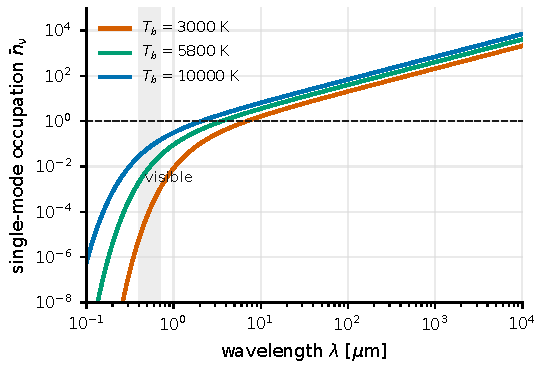
\includegraphics[width=0.82\linewidth]{figures/generated/chapter_03/ch03_blackbody_mode_occupation.pdf}
\caption{The single-mode occupation \(\bar n_\nu\) of three blackbodies of different brightness temperature (3000, 5800, 10000\,K) as a function of wavelength; the gray band marks the visible band, the dashed line marks \(\bar n_\nu=1\). Within the visible gray band, even at a brightness temperature of solar order, \(\bar n_\nu\) is far below 1 (\(\sim10^{-2}\)), showing that optical stellar light sits in the few-photon-per-mode regime; toward the long-wavelength (infrared, millimeter) end, the curves of each temperature cross the \(\bar n_\nu=1\) dashed line in turn, entering the strong-occupation, near-classical (Rayleigh--Jeans) limit of \(h\nu\ll k_{\rm B}T_b\).}
\label{fig:e05-mode-occupation}
\end{figure}

Why does this ``every mode is quite dim'' matter so much? Because it is precisely the starting point of the next several chapters. Since a coherence-time window usually contains no photon, and only occasionally one, what carries the spatial information of the celestial object is often the mode occupied by that single detected photon; this directly leads to the statistics of weak thermal light, the correlation of photons arriving in pairs, and the idea of quantum super-resolution beyond the diffraction limit. Carrying the sentence ``every mode of the Sun is actually quite dim,'' we can enter the next stage: seeing what statistical fingerprints these sparse photons leave on the detector.

\section{Chapter Summary}
\label{sec:e05-summary}

\begin{itemize}
  \item \textbf{Modes are the ``generalized pure tones'' of the light field.} Expanding the electromagnetic field along a set of orthogonal modes (frequency, spatial shape, polarization, time window) is a generalization of the Fourier idea to the electromagnetic field, with the benefit that each mode is independent and can be quantized separately.
  \item \textbf{Every mode is a harmonic oscillator.} This is the pivot of the whole chapter: the quantization of Chapter~\ref{chap:e04} is applied unchanged, giving the per-mode \(\hat a_k,\hat a_k^\dagger\), the commutation relation \([\hat a_i,\hat a_j^\dagger]=\delta_{ij}\), and the number operator \(\hat n_k=\hat a_k^\dagger\hat a_k\).
  \item \textbf{Photon = one excitation of some mode.} The only quantum ingredient in the positive-frequency field operator \(\hat E^{(+)}=\sum_k\mathcal E_k u_k(\bm r)e^{-i\omega_k t}\hat a_k\) is \(\hat a_k\); detecting one photon is decreasing the photon number in some mode by one. \(\hat E^{(-)}\) is its Hermitian conjugate.
  \item \textbf{The Fock state \(|\{N_k\}\rangle\)} pins down the photon number of every mode and is the coordinate basis for understanding all states of light.
  \item \textbf{An observing channel is often a sum of many modes}: \(M\simeq(\Delta t/\tau_c)(A\Omega/\lambda^2)N_{\rm pol}\), readily reaching thousands upon thousands in the visible.
  \item \textbf{Optical stellar light sits in the few-photon-per-mode regime}: \(\bar n_\nu=[\exp(h\nu/k_{\rm B}T_b)-1]^{-1}\), and at solar order \(\bar n_\nu\approx7\times10^{-3}\). A high total photon rate \(\neq\) many photons per mode.
\end{itemize}

\medskip
\noindent\textbf{Questions to Ponder.}
\begin{enumerate}
  \item If you widened the filter bandwidth \(\Delta\lambda\) by a factor of 10, how would the coherence time \(\tau_c\) and the number of time modes in a \(\Delta t\) time window each change?
  \item A thick fiber receiving a seeing-smeared image, versus a diffraction-limited imager, which has the larger spatial mode count \(A\Omega/\lambda^2\)? What does this mean for ``how deep the quantum fluctuations we see are''?
  \item For the same star, why does the ``few-photon-per-mode'' picture fail when observing at \(10\,\mu\mathrm{m}\) in the mid-infrared? Use \eqref{eq:e05-occupation} to estimate \(\bar n_\nu\) in this case.
\end{enumerate}


% ============================================================
\part{Quantum States of Light and Photon Statistics}
\chapter{Single-Mode States of Light: Number, Coherent, Thermal, and Squeezed States}
\label{chap:e06}

\begin{chapteropening}
In the previous chapter we accomplished something big: we decomposed the entire electromagnetic field into a bunch of modes and proved that \emph{every mode is mathematically a harmonic oscillator}; so ``photon'' obtained a precise definition, as one excitation of some mode. But the same mode, like the same spring, can be in a myriad of quantum states. The question this chapter answers is plain, and also crucial: \textbf{within the same mode, exactly which kinds of shape can light take on? What do they look like differently?} We will find that whether the photon number is pinned down, whether the phase is stable, and whether the intensity fluctuates, make four typical states of light (number, coherent, thermal, and squeezed) leave utterly different ``click-statistics fingerprints'' even when their mean photon number is identical. To measure all four kinds of light with a single measurement, we first build one unified ruler: the \emph{zero-delay pair factor} \(b_2\). Then, for each kind of light, we compute its \(b_2\) by hand: the number state gives \(1-1/n\) (antibunching), the coherent state gives \(1\) (the Poisson baseline), the thermal state gives \(2\) (bunching). This ``extra factor of two'' is precisely the seed on which the later intensity interferometry (Hanbury Brown--Twiss) relies to work.
\end{chapteropening}

\section{A Unified Ruler: The Zero-Delay Pair Factor}
\label{sec:e06-b2}

First let us be clear about exactly what we want to measure. Chapter~\ref{chap:e05} already told us that behind every ``click'' of a telescope stands an annihilation operator \(\hat a\): some mode has one photon fewer. If we fix our gaze on the same mode and ask ``how strong is the tendency for two clicks to arrive almost simultaneously,'' this is one of the most essential distinctions between states of light; it shows up not in how bright the average is, but in \emph{whether photons like to cluster}.

Anyone can compute the mean photon number; it is just the expectation of the number operator \(\langle\hat n\rangle\). But looking only at the mean, the number, coherent, and thermal states can be completely identical (all tuned to \(\langle\hat n\rangle=\bar n\)), yet they are three utterly different kinds of light. What truly separates them is the matter of ``pairing'': within the same mode, how many pairs of photons can be assembled?

\paragraph{Why the factorial moment, not the square}
\label{sec:e06-why-factorial}

A beginner's most natural thought is to use \(\langle\hat n^2\rangle\) to measure ``pairing.'' This is exactly the first pitfall this section sets out to correct. Suppose the mode has \(N\) photons at this moment, and we want to count ``how many \emph{ordered photon pairs} can be picked from them.'' There are \(N\) ways to pick the first photon, and to pick the second, since it must be \emph{another} photon, not the one just picked, there are only \(N-1\) ways left. So the number of ordered pairs is
\[
  N\times(N-1)=N(N-1),
\]
not \(N\times N=N^2\). The term by which the two differ, \(N^2-N(N-1)=N\), is precisely the spurious term of ``pairing the same photon with itself.'' Physically, \textbf{the same photon cannot pair with itself}: once a detector absorbs it, it is gone, and it cannot possibly be absorbed simultaneously by a second detector. So for any quantity involving ``two clicks,'' the correct count must be \(N(N-1)\), the so-called \emph{second factorial moment}. This reasoning of ``self-pairing must be subtracted'' will be proved again at the operator level when we discuss the normal ordering of photodetection in Chapter~\ref{chap:e07}; here we first accept it from the combinatorial meaning of ``counting pairs.''

And so we define the zero-delay pair factor:
\begin{equation}
  b_2\equiv\frac{\langle\hat n(\hat n-1)\rangle}{\langle\hat n\rangle^{2}} .
  \label{eq:e06-b2def}
\end{equation}
\begin{formulaexplain}
The numerator \(\langle\hat n(\hat n-1)\rangle\) is ``on average how many pairs of photons can be assembled'' (with self-pairing subtracted); the denominator \(\langle\hat n\rangle^2\) is ``the baseline number of pairs there should be if photons were independent and arrived at random.'' \(b_2\) is the ratio of the two: by how many times the tendency of photons to cluster is amplified relative to the random baseline.
\end{formulaexplain}

Let us account for each symbol. \(\hat n=\hat a^\dagger\hat a\) is the number operator, with eigenvalues \(N=0,1,2,\dots\) being pure integers with no units; \(\langle\cdot\rangle\) is the expectation over the light state (an inner product for a pure state, a trace \(\operatorname{Tr}(\rho\,\cdot)\) for a mixed state). The numerator \(\langle\hat n(\hat n-1)\rangle\) is unitless, the ``mean number of pairs''; the denominator \(\langle\hat n\rangle^2\) is also unitless. So \(b_2\) is a pure number; it does not care how bright the mode is (the denominator has already normalized the brightness away), only about \emph{whether the tendency of photons to arrive in pairs within the same mode is more or less than the random baseline of ``each independent, not communicating with the others.''}

Why does the baseline given by ``independent randomness'' make the numerator exactly equal to the denominator? The next section will verify it rigorously when we compute the coherent state. Here we first set out the three criteria, the yardstick against which this chapter repeatedly checks:
\begin{itemize}
  \item \(b_2=1\): the \textbf{independent Poisson baseline}. Photons each come on their own, not communicating; seeing one does not change the probability of immediately seeing another.
  \item \(b_2>1\): \textbf{bunching}. Photons like to cluster, ``come together if at all,'' with a pairing probability above the random baseline; thermal light is exactly so.
  \item \(b_2<1\): \textbf{antibunching}, also called \emph{sub-Poisson}. Photons avoid each other, ``having come once, another is not easily coming right away,'' with a pairing probability below the random baseline; this is a purely quantum effect that classical waves cannot achieve.
\end{itemize}

With this ruler, we ``measure'' the four kinds of light one by one. The strategy is always the same: first write down the photon-number distribution \(P(N)\) of that state (or its density matrix), compute \(\langle\hat n\rangle\) and \(\langle\hat n(\hat n-1)\rangle\), and substitute into \eqref{eq:e06-b2def}. Every step is shown.

\section{Number States: Light with Photon Number Pinned Down}
\label{sec:e06-fock}

We begin with the most ``clean-cut'' light. Chapter~\ref{chap:e05} already met the number state \(|n\rangle\), also called the Fock state: it is an eigenstate of the number operator, \(\hat n|n\rangle=n|n\rangle\), meaning this mode has \emph{exactly} \(n\) photons, not one more, not one fewer, with no fluctuation whatsoever. Its counting distribution is a single, lone vertical line:
\begin{equation}
  P(N)=\delta_{Nn}=
  \begin{cases}
    1, & N=n,\\
    0, & N\neq n.
  \end{cases}
  \label{eq:e06-fock-dist}
\end{equation}
\begin{formulaexplain}
\(P(N)\) is the probability of ``counting \(N\) photons''; \(\delta_{Nn}\) is the Kronecker delta, equal to 1 only when \(N=n\) and 0 otherwise. It says that measuring the photon number of a number state always yields the same value \(n\), with no fluctuation at all.
\end{formulaexplain}

Precisely because \(P(N)\) is nonzero only at \(N=n\), all expectations degenerate into ``directly substitute \(N=n\).'' The mean photon number is
\[
  \langle\hat n\rangle=\sum_{N}N\,P(N)=n\cdot 1=n,
\]
and the second factorial moment likewise retains only the \(N=n\) term:
\[
  \langle\hat n(\hat n-1)\rangle=\sum_{N}N(N-1)\,P(N)=n(n-1).
\]
Substituting into the definition of the pair factor \eqref{eq:e06-b2def}:
\begin{equation}
  b_{2,\text{Fock}}=\frac{n(n-1)}{n^{2}}=\frac{n-1}{n}=1-\frac{1}{n}.
  \label{eq:e06-fock-b2}
\end{equation}
\begin{formulaexplain}
The pair factor of a number state differs from the random baseline \(1\) by exactly \(1/n\). The fewer the photons, the more pronounced the antibunching; when \(n=1\), \(b_2\) is pressed all the way down to \(0\).
\end{formulaexplain}

This result is worth chewing over. For any finite \(n\), \(b_2=1-1/n<1\): the number state is always \emph{antibunched}. The reason is plain to see: the mode has only \(n\) photons, and using one to count a pair leaves one less in ``stock,'' so the number of pairs that can be assembled \(n(n-1)\) is naturally fewer than the \(n^2\) of ``independent randomness.'' In particular, take the single-photon state \(n=1\):
\[
  b_{2,\text{Fock}}(n=1)=1-\frac{1}{1}=0.
\]
This is the \emph{ideal limit} of antibunching. The physical meaning is decisive: a mode has only one photon, and it is gone once absorbed, so it can never let two detectors each receive one \emph{simultaneously}; hence the ``pairing'' probability is exactly zero. This is the most precious quantum signature of a single-photon source, and resonance fluorescence in the laboratory can clearly produce \(b_2\to 0\) \citep{1977PhRvL..39..691K}.

A reminder, though: astronomical light almost never arrives in a pure number state. The countless independent emitters in the source region, the long propagation path, and the telescope and detector all mix unobserved degrees of freedom in, pulling \(b_2\) from \(0\) all the way back toward \(1\). The value of the number state here is to give us a \emph{lower-bound anchor} and a reminder: click statistics measure the correlations of photon number, not a continuous waveform. When \(n\to\infty\), \(b_2\to 1\) and the antibunching disappears; once photons are numerous, the quantum ``exclusivity'' is drowned in the numbers, foretelling why bright celestial objects rarely display non-classical statistics.

\section{Coherent States: The Light Most Like a Classical Laser}
\label{sec:e06-coherent}

At the end of Chapter~\ref{chap:e04} we previewed a quantum state ``closest to classical vibration''; now we formally bring it on. The coherent state \(|\alpha\rangle\) is defined as an eigenstate of the annihilation operator:
\begin{equation}
  \hat a\,|\alpha\rangle=\alpha\,|\alpha\rangle,
  \qquad
  \bar n\equiv\langle\hat n\rangle=|\alpha|^{2}.
  \label{eq:e06-coherent-def}
\end{equation}
\begin{formulaexplain}
\(|\alpha\rangle\) satisfies ``after being acted on by the annihilation operator it is unchanged, merely multiplied by a complex number \(\alpha\).'' \(\alpha\) is a dimensionless complex amplitude: its squared modulus \(|\alpha|^2\) gives the mean photon number \(\bar n\), its argument \(\arg\alpha\) gives the phase. This is the quantum version of a phase-stable, definite-amplitude ``classical wave.''
\end{formulaexplain}

First let us explain why this definition is ``classical.'' \(\alpha\) is a dimensionless complex number, and you may picture it as that ``rotating arrow'' (complex amplitude) of Chapter~\ref{chap:e01}: the modulus \(|\alpha|\) is the amplitude, the argument is the phase, both definite, with no phase jitter; this is exactly the picture of an ideal laser. A stable laboratory laser is, in many measurements, extremely close to a coherent state \citep{1963PhRv..131.2766G}. And that peculiar property ``\(\hat a|\alpha\rangle=\alpha|\alpha\rangle\)'' means: \emph{removing one photon from a coherent state, it is still the same coherent state}, like scooping one drop from a vast wave of consistent phase, the ripples do not change at all. This is what fundamentally distinguishes it from the number state.

\paragraph{Deriving the Poisson distribution from the definition}
\label{sec:e06-coherent-poisson}

Chapter~\ref{chap:e04} twice previewed that ``the photon number of a coherent state follows a Poisson distribution''; here we \emph{derive} it from the definition rather than parachuting it in. The only raw material is the eigenvalue equation \eqref{eq:e06-coherent-def}, plus the annihilation-operator action rule of Chapter~\ref{chap:e05}, \(\hat a|N\rangle=\sqrt{N}\,|N-1\rangle\).

\textbf{Step one: write the coherent state as a superposition of number states.} The number states \(\{|N\rangle\}\) are a complete basis of this mode, so any single-mode state can be expanded as a linear combination of them. Let
\[
  |\alpha\rangle=\sum_{N=0}^{\infty}c_N\,|N\rangle,
\]
where the undetermined coefficient \(c_N=\langle N|\alpha\rangle\) is the amplitude of ``the \(N\)-photon component in this state.'' Substitute it into the left side of the eigenvalue equation, using \(\hat a|N\rangle=\sqrt{N}\,|N-1\rangle\) (note the \(N=0\) term is annihilated and does not contribute):
\[
  \hat a\,|\alpha\rangle
  =\sum_{N=1}^{\infty}c_N\sqrt{N}\,|N-1\rangle
  =\sum_{M=0}^{\infty}c_{M+1}\sqrt{M+1}\,|M\rangle,
\]
where the last step relabels with \(M\equiv N-1\). And the right side of the eigenvalue equation is
\[
  \alpha\,|\alpha\rangle=\sum_{M=0}^{\infty}\alpha\,c_M\,|M\rangle.
\]
\textbf{Step two: match coefficients number state by number state, obtaining a recursion.} Both sides are expansions in the number-state basis, so corresponding coefficients must be equal; thus for each \(M\):
\[
  c_{M+1}\sqrt{M+1}=\alpha\,c_M
  \quad\Longrightarrow\quad
  c_{M+1}=\frac{\alpha}{\sqrt{M+1}}\,c_M .
\]
\textbf{Step three: solve the recursion.} Climbing up rung by rung from \(c_0\), each added photon multiplies by an \(\alpha/\sqrt{N}\):
\[
  c_1=\frac{\alpha}{\sqrt1}c_0,\quad
  c_2=\frac{\alpha}{\sqrt2}c_1=\frac{\alpha^2}{\sqrt{2!}}c_0,\quad\dots\quad
  c_N=\frac{\alpha^{\,N}}{\sqrt{N!}}\,c_0 .
\]
\textbf{Step four: normalization fixes \(c_0\).} Require \(\langle\alpha|\alpha\rangle=\sum_N|c_N|^2=1\). Substituting the above and calling by name the exponential series \(\sum_{N}x^N/N!=e^{x}\) (here \(x=|\alpha|^2\)):
\[
  \sum_{N=0}^{\infty}|c_N|^2
  =|c_0|^2\sum_{N=0}^{\infty}\frac{|\alpha|^{2N}}{N!}
  =|c_0|^2\,e^{|\alpha|^2}=1
  \quad\Longrightarrow\quad
  |c_0|^2=e^{-|\alpha|^2}.
\]
Take the positive real \(c_0=e^{-|\alpha|^2/2}\) (the phase is free to choose, not affecting the probability). At this point the number-state expansion of the coherent state is completely determined. \textbf{Step five: read off the photon-number probability.} The probability of counting \(N\) photons is precisely the squared modulus of that component amplitude:
\begin{equation}
  P(N)=\big|\langle N|\alpha\rangle\big|^2=|c_N|^2
  =\frac{|\alpha|^{2N}}{N!}\,e^{-|\alpha|^2}
  =e^{-\bar n}\,\frac{\bar n^{\,N}}{N!},
  \qquad N=0,1,2,\dots
  \label{eq:e06-poisson}
\end{equation}
\begin{formulaexplain}
\(P(N)\) is the probability of counting \(N\) photons; \(\bar n=|\alpha|^2\) is the mean photon number; \(N!\) is the normalization of discrete counting. It is derived all the way from the eigenvalue equation, and it is exactly the ``independent random arrival'' Poisson distribution of Chapter~\ref{chap:e03}; the photons of a coherent state are independent, each coming on its own.
\end{formulaexplain}

The last step used \(\bar n=|\alpha|^2\), converting the complex amplitude into the mean photon number. Equation \eqref{eq:e06-poisson} is the \textbf{Poisson distribution}, and it is not asserted but forced out step by step from ``\(\hat a|\alpha\rangle=\alpha|\alpha\rangle\)'': the eigenvalue equation gives the recursion, the recursion gives the coefficients, normalization fixes the constant, and the squared modulus gives the probability. Here \(\bar n=|\alpha|^2\) is unitless, and \(N!\) is the factorial of \(N\). Equation \eqref{eq:e06-poisson} is \emph{exactly of the same form} as the Poisson distribution in Chapter~\ref{chap:e03} when we discussed shot noise; this is no coincidence: the photons of a coherent state are mutually independent random events, precisely the source of shot noise, with variance equal to mean \(\operatorname{Var}(N)=\bar n\).

\paragraph{Computing the pair factor of a coherent state by hand}
\label{sec:e06-coherent-b2}

Now measure it with the ruler. To compute \(b_2\), we need the second factorial moment \(\langle N(N-1)\rangle\). Substituting the Poisson distribution \eqref{eq:e06-poisson} into the sum, without omitting a step:
\[
  \langle N(N-1)\rangle
  =\sum_{N=0}^{\infty}N(N-1)\,e^{-\bar n}\frac{\bar n^{\,N}}{N!}.
\]
\textbf{Step one: cut off the terms that vanish.} Each term of the sum carries the factor \(N(N-1)\). When \(N=0\), \(N(N-1)=0\); when \(N=1\), \(N(N-1)=1\cdot 0=0\). So the \(N=0\) and \(N=1\) terms make \emph{no contribution} to the sum, and we can start summing directly from \(N=2\):
\[
  \langle N(N-1)\rangle
  =\sum_{N=2}^{\infty}N(N-1)\,e^{-\bar n}\frac{\bar n^{\,N}}{N!}.
\]
\textbf{Step two: cancel the factorial.} Note the definition of the factorial \(N!=N(N-1)(N-2)!\), so \(N(N-1)/N!=1/(N-2)!\). This step cleanly eliminates the obstructive \(N(N-1)\):
\[
  \langle N(N-1)\rangle
  =e^{-\bar n}\sum_{N=2}^{\infty}\frac{\bar n^{\,N}}{(N-2)!}.
\]
\textbf{Step three: change variables in the sum.} Let \(m\equiv N-2\) (so \(N=2\) corresponds to \(m=0\), and \(N\to\infty\) corresponds to \(m\to\infty\)), and split \(\bar n^{\,N}=\bar n^{\,2}\cdot\bar n^{\,m}\), pulling the sum-independent \(\bar n^2\) outside:
\[
  \langle N(N-1)\rangle
  =e^{-\bar n}\,\bar n^{2}\sum_{m=0}^{\infty}\frac{\bar n^{\,m}}{m!}.
\]
\textbf{Step four: use the exponential series.} That last sum is exactly the Taylor series of the exponential function \(\sum_{m=0}^{\infty}\bar n^{\,m}/m!=e^{\bar n}\), a standard result we call by name. So \(e^{-\bar n}\) and \(e^{\bar n}\) cancel exactly:
\[
  \langle N(N-1)\rangle
  =e^{-\bar n}\,\bar n^{2}\,e^{\bar n}
  =\bar n^{2}.
\]
Clean and neat. Since \(\langle N\rangle=\bar n\), substituting into the definition of the pair factor \eqref{eq:e06-b2def}:
\begin{equation}
  b_{2,\text{coh}}=\frac{\langle N(N-1)\rangle}{\langle N\rangle^{2}}
  =\frac{\bar n^{2}}{\bar n^{2}}=1.
  \label{eq:e06-coherent-b2}
\end{equation}
\begin{formulaexplain}
The pair factor of a coherent state is exactly \(1\), independent of the brightness \(\bar n\). It is the \emph{independent Poisson baseline} on our yardstick: photons each come on their own, with a pairing probability neither more nor less.
\end{formulaexplain}

This \(b_2=1\) is the rigorous source of the ``independent random baseline'' in \eqref{eq:e06-b2def}. Physically it says something very plain: \textbf{seeing one photon in a coherent state does not change the conditional probability of immediately seeing another}. Photons neither communicate, nor pair up, nor avoid one another; they are purely independent. This also explains why a coherent state is neither bunched nor antibunched; it sits exactly on the dividing line between classical and quantum, the ``most classical quantum state.'' A stable laser is approximately so; but beware, \emph{a celestial narrow-line or high-brightness-temperature source is not automatically a coherent state}: independent emitting regions, turbulent velocity fields, and multiple scattering paths all smear the phase, and the result is instead closer to the thermal state of the next section.

\section{Thermal States: The Light of Stellar Continua}
\label{sec:e06-thermal}

Now for the light that astronomers most often deal with. The single-mode statistics of stellar continua, the scattered light of interplanetary dust, and the vast majority of incoherent sources all start from the thermal state. It has no fixed phase and is a \emph{mixed state} in the photon-number basis, with density matrix
\begin{equation}
  \rho_{\text{th}}=\sum_{N=0}^{\infty}
  \frac{\bar n^{\,N}}{(1+\bar n)^{\,N+1}}\,|N\rangle\langle N|,
  \label{eq:e06-thermal-rho}
\end{equation}
\begin{formulaexplain}
\(\rho_{\text{th}}\) is the thermal-state density matrix; it is an \emph{incoherent} mixture of the number states \(|N\rangle\), with weights decreasing geometrically; \(\bar n\) is the mean occupation of this mode. The thermal state has no phase information, only ``the probability of each photon number occurring.''
\end{formulaexplain}

First understand this expression. \(|N\rangle\langle N|\) is the operator projecting onto ``exactly \(N\) photons,'' and the coefficient in front is the probability of counting \(N\) photons
\[
  P(N)=\frac{\bar n^{\,N}}{(1+\bar n)^{\,N+1}}
  =\frac{1}{1+\bar n}\left(\frac{\bar n}{1+\bar n}\right)^{N}.
\]
This is a \textbf{geometric distribution}, that is, the Bose--Einstein distribution encountered when deriving the boson occupation in Chapter~\ref{chap:e05}: the probability decreases monotonically with \(N\), but drags a long tail of high photon number. It is precisely this tail that makes thermal light like to ``cluster'' more than coherent light. To verify normalization, use the geometric-series sum \(\sum_{N=0}^\infty q^N=1/(1-q)\) (here the common ratio \(q=\bar n/(1+\bar n)<1\), convergent), giving \(\sum_N P(N)=\frac{1}{1+\bar n}\cdot\frac{1}{1-q}=\frac{1}{1+\bar n}\cdot(1+\bar n)=1\), correct.

\paragraph{Computing the pair factor of a thermal state by hand}
\label{sec:e06-thermal-b2}

We want two things: the mean \(\langle N\rangle\) and the second factorial moment \(\langle N(N-1)\rangle\). Both start from the geometric distribution and are computed directly with the ready-made trick of ``differentiating the geometric series term by term'' from Chapter~\ref{chap:e05}, without borrowing any outside help; the variance \(\operatorname{Var}(N)\) is then read off as a by-product to explain the physics of bunching.

\textbf{The mean.} This step was already computed in Chapter~\ref{chap:e05} with the ``differentiate the geometric series term by term'' trick, the conclusion being
\[
  \langle N\rangle=\sum_{N=0}^{\infty}N\,P(N)=\bar n.
\]
That is, the parameter \(\bar n\) in \eqref{eq:e06-thermal-rho} lives up to its name and is exactly the mean photon number.

\textbf{The second factorial moment: computed directly by differentiating the geometric distribution term by term.} This is the core quantity of this section, and we do not borrow any unproven variance but compute it term by term from the geometric distribution \eqref{eq:e06-thermal-rho}, by the same method as the ``differentiate the geometric series'' used for the mean in Chapter~\ref{chap:e05}. For clean notation, write the common ratio
\[
  q\equiv\frac{\bar n}{1+\bar n}\in(0,1),
  \qquad\text{so that}\quad 1-q=\frac{1}{1+\bar n},\quad P(N)=(1-q)\,q^{N}.
\]
Everything starts from the most basic geometric series (convergent only for common ratio \(|q|<1\), satisfied here):
\[
  \sum_{N=0}^{\infty}q^{N}=\frac{1}{1-q}.
\]
Differentiating both sides once with respect to \(q\) gives that one formula used for the mean in Chapter~\ref{chap:e05}, \(\sum_N N q^{N-1}=1/(1-q)^2\); we here \emph{differentiate once more}, ``knocking'' the \(N(N-1)\) out of the power:
\[
  \frac{d^{2}}{dq^{2}}\sum_{N=0}^{\infty}q^{N}
  =\sum_{N=0}^{\infty}N(N-1)\,q^{\,N-2}
  =\frac{2}{(1-q)^{3}} .
\]
This step calls by name a standard result: \emph{for a convergent power series, term-by-term differentiation and summation can be interchanged} (for \(0<q<1\) the series converges uniformly in a neighborhood of \(q\), so it is legitimate). The right-hand side is obtained by differentiating \((1-q)^{-1}\) twice. Multiplying both sides by \(q^{2}\), restoring the power to \(q^{N}\):
\[
  \sum_{N=0}^{\infty}N(N-1)\,q^{N}=\frac{2q^{2}}{(1-q)^{3}} .
\]
Now equipping each term with the leading normalization factor \((1-q)\) gives the expectation we want:
\[
  \langle N(N-1)\rangle
  =(1-q)\sum_{N=0}^{\infty}N(N-1)\,q^{N}
  =(1-q)\cdot\frac{2q^{2}}{(1-q)^{3}}
  =\frac{2q^{2}}{(1-q)^{2}}
  =2\left(\frac{q}{1-q}\right)^{2}.
\]
Finally convert \(q\) back to \(\bar n\): from \(q=\bar n/(1+\bar n)\) and \(1-q=1/(1+\bar n)\) we get \(q/(1-q)=\bar n\), so
\begin{equation}
  \langle N(N-1)\rangle=2\bar n^{2}.
  \label{eq:e06-thermal-fm}
\end{equation}
\begin{formulaexplain}
The second factorial moment of a thermal state is \(2\bar n^2\), exactly \emph{twice} the \(\bar n^2\) of a coherent state. This extra factor of two is the entire source of the later \(b_2=2\) (bunching); it is computed by hand by differentiating the geometric distribution term by term, without invoking any unproven fact.
\end{formulaexplain}

\textbf{Read off the variance in passing, to make bunching clear.} Since the factorial moment is now in hand, the variance is its direct by-product: using \(\langle N^2\rangle=\langle N(N-1)\rangle+\langle N\rangle\),
\begin{equation}
  \operatorname{Var}(N)=\langle N^{2}\rangle-\langle N\rangle^{2}
  =\big[2\bar n^{2}+\bar n\big]-\bar n^{2}
  =\bar n+\bar n^{2}=\bar n(1+\bar n).
  \label{eq:e06-thermal-var}
\end{equation}
\begin{formulaexplain}
The variance of a thermal state exceeds the Poisson \(\bar n\) by one term \(\bar n^2\). The first term \(\bar n\) is the unavoidable shot noise (``photons come one at a time''), and the second term \(\bar n^2\) is the \emph{intensity fluctuation} peculiar to thermal light, precisely what brings bunching.
\end{formulaexplain}

Read the variance \eqref{eq:e06-thermal-var} split into two parts: \(\operatorname{Var}(N)=\underbrace{\bar n}_{\text{shot noise}}+\underbrace{\bar n^{2}}_{\text{intensity fluctuation}}\). The first term \(\bar n\), as in the coherent state, is the unavoidable shot noise from ``photons being discrete''; the second term \(\bar n^2\) is the \emph{extra} that the thermal state carries, coming from the intensity of the light field itself fluctuating randomly: thermal light is sometimes bright, sometimes dim, and when bright the photons all become more numerous together, when dim they all become fewer together. This ``excess variance'' is the root of bunching; please remember it. With the factorial moment \eqref{eq:e06-thermal-fm}, substitute directly into the definition of the pair factor \eqref{eq:e06-b2def}:
\begin{equation}
  b_{2,\text{th}}=\frac{\langle N(N-1)\rangle}{\langle N\rangle^{2}}
  =\frac{2\bar n^{2}}{\bar n^{2}}=2.
  \label{eq:e06-thermal-b2}
\end{equation}
\begin{formulaexplain}
The pair factor of a thermal state is exactly \(2\), independent of brightness. It is \emph{twice} the random baseline: the probability of thermal-light photons arriving in pairs is twice that of the independent random case. This is bunching.
\end{formulaexplain}

This \(b_2=2\) is the centerpiece of this chapter. Where does that ``extra factor'' (the \(1\) by which \(2\) exceeds the baseline \(1\)) come from? It is \emph{not} a detector effect, nor some new particle interaction, but the direct consequence of that second intensity-fluctuation term \(\bar n^2\) above: when thermal light has excess intensity in some short coherence time, multiple photons \emph{together} more easily arrive; when intensity is low, they \emph{together} become fewer. This ``all more together, or all fewer together'' advance-and-retreat in unison makes photons tend to arrive in pairs and in groups; this is the microscopic picture of bunching.

The importance of this cannot be overstated: \textbf{the \(b_2=2\) of thermal light is precisely the seed on which Hanbury Brown--Twiss (intensity interferometry) relies to work}. In the 1950s Hanbury Brown and Twiss, by measuring exactly this excess correlation of photon arrival on two detectors, first measured stellar angular diameters without amplitude interferometry \citep{1956Natur.177...27B,1957RSPSA.242..300B}. Without that extra factor of thermal light, there would be no measurable correlation peak. In Chapter~\ref{chap:e08} we will translate this \(b_2=2\) precisely into the second-order coherence function \(g^{(2)}(0)=2\), and in Chapter~\ref{chap:e10} turn it into a tool for measuring angular diameters.

One necessary reminder: the \(\bar n\) here is the \emph{single-mode} mean occupation, not the total photon rate the telescope receives per second. Moreover, a real observation is always a sum of many modes (the \(M\) of Chapter~\ref{chap:e05}), and the multi-mode average dilutes this ``excess variance,'' making the measured bunching contrast smaller than the single-mode ideal of \(2\). This dilution effect is also a core matter to be handled repeatedly in Chapters~\ref{chap:e08} and \ref{chap:e10}.

Figure~\ref{fig:e06-count-distributions} draws the counting distributions of the three kinds of light at the same mean photon number together, and the source of the difference is seen at a glance.

\begin{figure}[tbp]
\centering
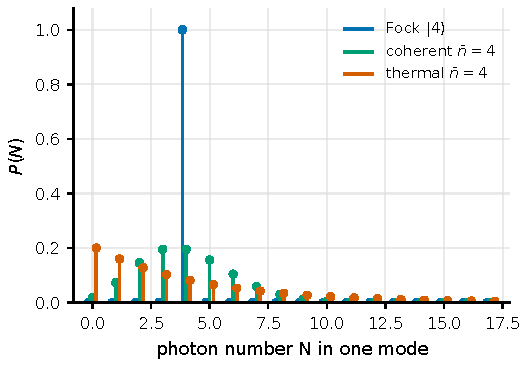
\includegraphics[width=0.82\linewidth]{figures/generated/chapter_03/ch03_state_count_distributions.pdf}
\caption{Near the same mean photon number, the number, coherent, and thermal states give completely different counting distributions \(P(N)\). The number state is a single pinned-down vertical line (no fluctuation in photon number, \(b_2=1-1/n<1\)); the coherent state is a Poisson distribution, with width about \(\sqrt{\bar n}\) (\(b_2=1\)); the thermal state is a geometric distribution, dragging a long tail of high photon number (\(b_2=2\), bunching). It is precisely this tail that makes thermal light more likely to arrive ``in pairs'' at zero delay.}
\label{fig:e06-count-distributions}
\end{figure}

The lesson of Figure~\ref{fig:e06-count-distributions} is extremely simple: \emph{the mean photon number is not everything}. The number state has no photon-number fluctuation, the coherent state has Poisson fluctuation, and the thermal state additionally bears a layer of intensity fluctuation. What astronomical intensity interferometry exploits is precisely this last layer of fluctuation of the thermal state.

\section{Squeezed States: Relocating the Quantum Noise}
\label{sec:e06-squeezed}

The first three kinds of light concerned ``how the photon number is distributed.'' The squeezed state is about something different: \emph{quantum noise can be redistributed between two orthogonal field components}. It does not change the language of photon-pairing statistics but returns to the quadrature picture of Chapter~\ref{chap:e04}.

First define a quadrature operator at a phase angle \(\theta\):
\begin{equation}
  \hat X_\theta=\frac{1}{2}\left(\hat a\,e^{-i\theta}+\hat a^{\dagger}e^{i\theta}\right).
  \label{eq:e06-quadrature}
\end{equation}
\begin{formulaexplain}
\(\hat X_\theta\) is the ``projection'' of the field along the phase direction \(\theta\), a generalization of the position/momentum operators of Chapter~\ref{chap:e04}: \(\theta=0\) gives the ``position''-like component, \(\theta=\pi/2\) gives the ``momentum''-like component. It is dimensionless and measures the coordinate of the field along some direction in phase space.
\end{formulaexplain}

Let us account for each. \(\hat X_\theta\) is dimensionless; \(\theta\) is the phase-space ``viewing angle'' we choose (in radians); \(\hat a,\hat a^\dagger\) are old acquaintances. Taking \(\theta=0\) gives \(\hat X_0=\tfrac12(\hat a+\hat a^\dagger)\), proportional to the position operator \(\hat x\) of Chapter~\ref{chap:e04}; taking \(\theta=\pi/2\) gives \(\hat X_{\pi/2}=\tfrac{1}{2i}(\hat a-\hat a^\dagger)\), proportional to the momentum operator \(\hat p\). These two orthogonal directions are the ``horizontal and vertical axes'' of phase space.

The key quantum fact is: \textbf{the vacuum state (and any coherent state) has equal fluctuation in every direction}, with variance \(1/4\) in all. This baseline value is not hard to compute, and it is worth cashing out on the spot: it uses only two properties of the vacuum, \(\hat a|0\rangle=0\) and the commutation relation \([\hat a,\hat a^\dagger]=1\). In the vacuum \(\langle\hat X_\theta\rangle=0\) (the expectations of both \(\hat a,\hat a^\dagger\) are zero), so the variance equals \(\langle\hat X_\theta^2\rangle\). Expanding the square of the definition \eqref{eq:e06-quadrature}:
\[
  \hat X_\theta^{2}
  =\frac14\big(\hat a\,e^{-i\theta}+\hat a^\dagger e^{i\theta}\big)^2
  =\frac14\big(\hat a^2 e^{-2i\theta}+\hat a^{\dagger 2}e^{2i\theta}
     +\hat a\hat a^\dagger+\hat a^\dagger\hat a\big).
\]
Take the vacuum expectation term by term: the term with \(\hat a^2\) vanishes because \(\hat a|0\rangle=0\); the term with \(\hat a^{\dagger2}\), its Hermitian conjugate, likewise vanishes; \(\hat a^\dagger\hat a\,|0\rangle=0\) (the number operator acting on the vacuum is zero); only \(\langle 0|\hat a\hat a^\dagger|0\rangle\) remains, and using \(\hat a\hat a^\dagger=\hat a^\dagger\hat a+[\hat a,\hat a^\dagger]=\hat n+1\) gives \(\langle0|\hat a\hat a^\dagger|0\rangle=0+1=1\). So
\[
  \Delta X_\theta^{2}\big|_{\text{vacuum}}=\langle\hat X_\theta^2\rangle
  =\frac14\cdot 1=\frac{1}{4}\qquad(\text{for all }\theta).
\]
The result is independent of \(\theta\), showing precisely that the vacuum is an isotropic ``circular blob'' in phase space; this is also the starting point of the next section's phase-space picture. The Heisenberg uncertainty requires the product of the variances of two orthogonal directions to be no less than \(\tfrac{1}{16}\), and the vacuum saturates this minimum exactly (\(\tfrac14\times\tfrac14=\tfrac1{16}\)).

What the squeezed state does is \emph{squash} this circular blob: pressing the variance along some direction below \(1/4\), at the cost of the variance of the conjugate direction being correspondingly raised. Let the squeezing parameter be \(r\ge0\); then
\begin{equation}
  \Delta X_{\text{sq}}^{2}=\frac{1}{4}\,e^{-2r},
  \qquad
  \Delta X_{\text{anti}}^{2}=\frac{1}{4}\,e^{+2r}.
  \label{eq:e06-squeeze-var}
\end{equation}
\begin{formulaexplain}
The variance of the squeezed direction is multiplied by \(e^{-2r}<1\) (noise decreases), and the variance of the anti-squeezed direction is multiplied by \(e^{+2r}>1\) (noise increases). The larger \(r\), the ``flatter'' one direction and the ``fatter'' the other.
\end{formulaexplain}

This \(e^{\mp 2r}\) shape comes from the single-mode squeezing transformation: it multiplies the amplitude scale of phase space along one quadrature direction by \(e^{-r}\), so the variance (the square of the scale) is multiplied by \(e^{-2r}\); the scale of the conjugate direction is multiplied by \(e^{+r}\), the variance by \(e^{+2r}\). Most crucial is multiplying the two variances together:
\[
  \Delta X_{\text{sq}}^{2}\cdot\Delta X_{\text{anti}}^{2}
  =\frac14 e^{-2r}\cdot\frac14 e^{+2r}
  =\frac{1}{16}\,e^{-2r+2r}
  =\frac{1}{16}.
\]
The product is \emph{still} \(1/16\), exactly the same as the vacuum! This sentence is the key to understanding squeezing: \textbf{squeezing has not eliminated the quantum noise; it has merely moved the noise from one direction to another}: press down the gourd and the ladle pops up, the total conserved. You may make some quadrature component quieter than the vacuum, but you must let its conjugate component grow noisy to compensate.

The experimental literature often uses decibels (dB) to note the noise ratio relative to vacuum: \(10\log_{10}(e^{-2r})\). For example, a noise variance reduced to one tenth of the vacuum is \(-10\,\text{dB}\). Modern squeezed-light experiments near \(1064\,\text{nm}\) can already stably produce \(10\)--\(15\,\text{dB}\) of noise reduction, and it has been used in gravitational-wave detectors to press shot noise below the standard quantum limit \citep{1983Natur.306..141W,2016PhRvL.117k0801V}.

But a cold splash of water for astronomy: \textbf{ordinary stellar continua do not carry squeezing by default}. Thermal and coherent states have fluctuations no smaller than vacuum in every quadrature direction; there is no ``squashing'' to speak of. Squeezing is a non-classical state that must be carefully prepared with nonlinear optical processes (such as parametric down-conversion), and natural thermal sources like stars and nebulae do not produce it spontaneously. We introduce the squeezed state, first, to complete the full atlas of ``which kinds of light the same mode can hold,'' and second, because it is crucial on the \emph{instrument side}: future quantum-enhanced telescope back ends may use squeezed light to break through shot noise. But treating it as the default model of astronomical light is a misconception to avoid.

\section{The Weak Thermal Light Limit: A Line Laid Down for Super-Resolution}
\label{sec:e06-weak}

The last section pushes the thermal state into the most common corner of astronomy: \emph{every mode is actually quite dim}. Chapter~\ref{chap:e05} computed that in the visible the single-mode occupation of a star is \(\bar n_\nu\sim10^{-2}\ll1\). In this weak thermal light limit, the thermal state degenerates into a particularly simple, particularly useful form.

Starting from the geometric distribution, expand \(P(N)\) to lowest order when \(\bar n\ll 1\). The probability of zero photons is
\[
  P(0)=\frac{1}{1+\bar n}\simeq 1-\bar n+\mathcal O(\bar n^{2}),
\]
where we used the geometric-series expansion \((1+\bar n)^{-1}=1-\bar n+\bar n^2-\cdots\) (convergent for \(\bar n<1\)), keeping only to first order. The probability of one photon is
\[
  P(1)=\frac{\bar n}{(1+\bar n)^{2}}
  \simeq\bar n\,(1-2\bar n+\cdots)
  \simeq\bar n+\mathcal O(\bar n^{2}).
\]
The probability of two or more photons is
\[
  P(N\ge 2)=\mathcal O(\bar n^{2}),
\]
because \(P(2)=\bar n^2/(1+\bar n)^3\sim\bar n^2\), a higher-order small quantity. That is, in weak thermal light \emph{the vast majority of coherence-time windows are empty}, occasionally one window has one photon popping out, while two photons in the same window is a second-order rare event.

Writing this hierarchy as a density matrix gives the standard bookkeeping form of weak thermal light:
\begin{equation}
  \rho\simeq(1-\varepsilon)\,\rho_0+\varepsilon\,\rho_1+\mathcal O(\varepsilon^{2}),
  \qquad
  \varepsilon\equiv\bar n\ll 1,
  \label{eq:e06-weak}
\end{equation}
\begin{formulaexplain}
\(\rho_0=|0\rangle\langle 0|\) is the vacuum part (fraction \(1-\varepsilon\)), \(\rho_1=|1\rangle\langle 1|\) is the one-photon part (fraction \(\varepsilon\)), and \(\varepsilon=\bar n\) is the single-mode mean photon number. Weak thermal light is a sparse photon stream that is ``mostly empty, occasionally one.''
\end{formulaexplain}

Let us account for each: \(\rho_0\) is the density matrix of the vacuum state, \(\rho_1\) is the density matrix of the single-photon state, and the small parameter \(\varepsilon=\bar n\) is dimensionless, exactly equal to the lowest-order \(P(1)\) above, so \emph{it is exact to identify \(\varepsilon\) as ``the mean photon number of that mode in that time window.''} Equation \eqref{eq:e06-weak} says: the light state is almost entirely vacuum, with just a tiny bit of single-photon component mixed in. This ``tiny bit'' is precisely what carries the celestial information.

Why devote a whole section to it? Because it is the starting point of the later \textbf{quantum super-resolution}. Since a coherence-time window usually contains no photon and only occasionally one, what truly carries the spatial information of the celestial object is the spatial structure of that \emph{one-photon mode} that was detected. The weak-thermal-light super-resolution theory of Tsang, Nair, and Lu starts precisely from an expansion like \eqref{eq:e06-weak}, proving that as long as one can cleverly measure the mode of this single photon (rather than simply counting the intensity), one can break through the classical Rayleigh limit \citep{2015Optic...2..646T,2016PhRvX...6c1033T}. We will pick up this line in Chapter~\ref{chap:e12}, discussing how SPADE (spatial-mode demultiplexing) approaches the resolution limit of two stars extremely close together. This also fits naturally with the astronomical event table: the time windows of zero photons are never stored in the file at all; what remains in the data are those sparse single-photon clicks with time stamps.

\section{The Phase-Space Picture: Drawing the Four Kinds of Light on One Diagram}
\label{sec:e06-phasespace}

Let us gather this chapter onto one \emph{visible} diagram. Phase space uses two quadrature components \(X\) (horizontal axis) and \(P\) (vertical axis) to span a plane, drawing the quantum state of a mode as a ``probability cloud'' on this plane: the center of the cloud is the mean field, the fatness of the cloud is the fluctuation. As said in the previous section, the vacuum and coherent states have fluctuations of \(1/4\) in every direction, so they draw as an isotropic \emph{circular blob}. The four kinds of light each have their own look on this diagram:

\begin{itemize}
  \item \textbf{Vacuum state}: a circular blob at the origin, its radius set by the \(1/4\) fluctuation. This is the ``base'' of all noise.
  \item \textbf{Coherent state}: a circular blob \emph{of exactly the same size}, only translated to a distance \(|\alpha|\) from the origin. It moves the vacuum's circular blob as a whole, shape unchanged; so the coherent state is a ``displaced vacuum,'' with noise as small and as isotropic as the vacuum. This corresponds to its \(b_2=1\).
  \item \textbf{Thermal state}: a \emph{fatter circle still centered at the origin}. It has no fixed phase (the argument is completely random) and has intensity fluctuation, so the probability cloud spreads out in all directions, its radius growing with \(\bar n\). This ``fatter'' is precisely the phase-space image of the thermal state's extra variance \(\bar n^2\), also corresponding to its \(b_2=2\).
  \item \textbf{Squeezed state}: a \emph{squashed ellipse}. Along the squeezed direction it is narrow, below vacuum (\(\tfrac14 e^{-2r}\)), and along the conjugate direction it is propped fat (\(\tfrac14 e^{+2r}\)), but the area of the ellipse (the variance product \(1/16\) corresponding to the product of the two semi-axes) is the same as the circular blob: ``noise relocated, area conserved'' appears on the diagram as ``circle squashed into an equal-area ellipse.''
\end{itemize}

Figure~\ref{fig:e06-phase-space} draws these three ``clouds'' of the coherent, thermal, and squeezed states side by side.

\begin{figure}[tbp]
\centering
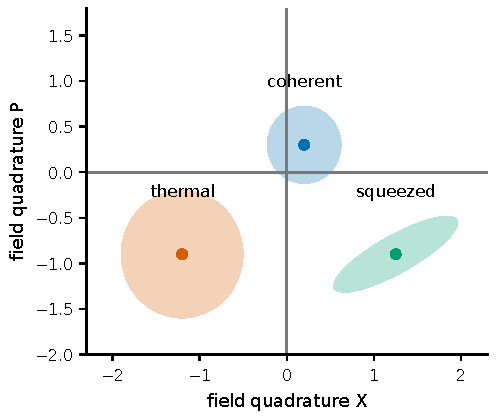
\includegraphics[width=0.72\linewidth]{figures/generated/chapter_03/ch03_phase_space_states.pdf}
\caption{The fluctuation shapes of three kinds of single-mode light state in phase space. The coherent state is a circular blob the same size as the vacuum, only translated (a ``displaced vacuum''); the thermal state, due to random phase and intensity fluctuation, spreads into a fatter circle; the squeezed state presses the fluctuation of one quadrature direction below vacuum while raising the conjugate direction, becoming an equal-area ellipse. Remember: what distinguishes different states of light is, first of all, the \emph{shape} of the fluctuations and correlations, not just the mean intensity.}
\label{fig:e06-phase-space}
\end{figure}

This phase-space diagram gives one take-away sentence: \emph{the distinction between different states of light shows up, first of all, as the shape of the fluctuations and correlations, not just the mean intensity}. The same brightness can be a well-behaved circular blob (coherent state), a restless fat circle (thermal state), or a squashed ellipse (squeezed state), and it is precisely these shapes that determine the pairing statistics of clicks on the detector. Carrying this diagram, we can enter Chapter~\ref{chap:e07} and see how these states of light truly become a string of analyzable events on a photodetector.

\section{Chapter Summary}
\label{sec:e06-summary}

\begin{itemize}
  \item \textbf{The ruler: the zero-delay pair factor} \(b_2=\langle\hat n(\hat n-1)\rangle/\langle\hat n\rangle^2\). The numerator uses the factorial moment \(\hat n(\hat n-1)\) rather than \(\hat n^2\), because ``the same photon cannot pair with itself'' and self-pairing must be subtracted. \(b_2=1\) is the independent Poisson baseline, \(>1\) bunching, \(<1\) antibunching (non-classical).
  \item \textbf{Number state \(|n\rangle\)}: \(P(N)=\delta_{Nn}\), photon number pinned down. \(\langle\hat n\rangle=n\), \(\langle\hat n(\hat n-1)\rangle=n(n-1)\), giving \(b_2=1-1/n<1\). The single photon \(n=1\) gives \(b_2=0\), the ideal limit of antibunching.
  \item \textbf{Coherent state \(|\alpha\rangle\)}: \(\hat a|\alpha\rangle=\alpha|\alpha\rangle\), \(\bar n=|\alpha|^2\), counting is Poisson. Term-by-term summation (cut off zero terms, cancel the factorial, change variables, use the exponential series) gives \(\langle N(N-1)\rangle=\bar n^2\), so \(b_2=1\). Seeing one photon does not change the probability of immediately seeing another.
  \item \textbf{Thermal state \(\rho_{\text{th}}\)}: geometric/Bose distribution, \(\langle N\rangle=\bar n\), \(\operatorname{Var}=\bar n(1+\bar n)\), \(\langle N(N-1)\rangle=2\bar n^2\), so \(b_2=2\). The extra factor comes from intensity fluctuation (more together when bright, fewer together when dim), precisely the seed of Hanbury Brown--Twiss bunching.
  \item \textbf{Squeezed state}: quadrature \(\hat X_\theta=\tfrac12(\hat a e^{-i\theta}+\hat a^\dagger e^{i\theta})\), vacuum variance \(1/4\); squeezed/anti-squeezed variance \(\tfrac14 e^{\mp 2r}\), the product still \(1/16\): the noise is relocated, not eliminated. Ordinary stellar light does not carry squeezing by default; it is mainly useful on the instrument side.
  \item \textbf{Weak thermal light limit}: for \(\bar n\ll1\), \(\rho\approx(1-\varepsilon)\rho_0+\varepsilon\rho_1\), \(\varepsilon=\bar n\), obtained from the lowest-order geometric distribution \(P(0)\approx1-\bar n\), \(P(1)\approx\bar n\). Most time windows are empty, and what carries the spatial information is that detected single-photon mode, leading to the super-resolution of Chapter~\ref{chap:e12}.
  \item \textbf{Phase space}: coherent state = displaced vacuum circular blob, thermal state = fatter circle, squeezed state = equal-area flat ellipse. What distinguishes states of light is, first of all, the shape of the fluctuations, not the mean intensity.
\end{itemize}

\medskip
\noindent\textbf{Questions to Ponder.}
\begin{enumerate}
  \item If you incoherently superpose two independent single-mode thermal beams (each with \(b_2=2\)) into one ``two-mode'' channel, will the observed pair factor be greater than 2, equal to 2, or less than 2? Is this consistent with the ``multi-mode dilution'' statement of Chapter~\ref{chap:e05}?
  \item For the same mean photon number \(\bar n=10\), what are the counting variances of the number, coherent, and thermal states? Which is the ``quietest'' and which the ``noisiest''?
  \item If some celestial source is measured to have \(b_2<1\), can you immediately assert it is a non-classical source? Before drawing the conclusion, which instrumental and mixing effects that could raise or lower \(b_2\) must you still rule out (recall the mode count \(M\) of Chapter~\ref{chap:e05})?
\end{enumerate}

\chapter{Photodetection and Photon Counting: Why We Count n(n-1)}
\label{chap:e07}

\begin{chapteropening}
Up to the previous chapter, we had ``read'' light very thoroughly: light is a set of mode excitations, every mode is a harmonic oscillator, a photon is one portion of energy in a mode, and the number, coherent, and thermal states (even at the same brightness) have utterly different tendencies \(b_2\) for photons to arrive in pairs (Chapter~\ref{chap:e06}). But all of this still stayed on the ``light state'' side. What the telescope side hands back is never a wave function, but a string of cold clicks: at some moment, at some pixel, a snap. What this chapter builds is precisely the bridge between these two sides: how exactly does a light state become a string of counts on a detector? We will work out three things step by step. First, why ``detecting one photon,'' mathematically, forces us to count \(n(n-1)\) rather than \(n^2\): that subtracted \(n\) is precisely ``the same photon cannot pair with itself.'' Second, how to slice an event table into time gates and, with a number called the Mandel \(Q\), see at a glance whether this beam of light ``clusters'' more than Poisson or is more ``orderly.'' Third, why the majestic \(g^{(2)}(0)=2\) of the textbooks shrinks, on a real telescope, into a small number like \(1+10^{-3}\) or even \(1+10^{-6}\): not that the signal is gone, but that it has been diluted by thousands upon thousands of modes. By the end of this chapter, you will hold the full conversion from ``the quantum state of light'' to ``count statistics that can truly be taken and fitted.''
\end{chapteropening}

\section{Where Clicks Come From: Detection Is Absorbing One Photon}
\label{sec:e07-absorption}

Let us return to the plainest question: when a detector ``sees'' one photon, what physically happens?

It is not that a photon hits a wall and bounces back, nor that it is ``caught'' like a little ball. Real photodetection is an \emph{absorption}: one portion of energy in the light field is handed to the detector (knocking out a photoelectron, triggering an avalanche, flipping a pixel), and at the same time \textbf{the light field has one photon fewer}. In Chapter~\ref{chap:e05} we already stressed this sentence repeatedly and wrote it in operator language: absorption uses only the positive-frequency field operator \(\hat E^{(+)}\), because \(\hat E^{(+)}\) carries the annihilation operator \(\hat a\) (removing one photon), not the creation operator \(\hat a^\dagger\).

Now fix attention on a single mode. Here the positive-frequency field is proportional to that mode's annihilation operator, \(\hat E^{(+)}\propto\hat a\). Quantum detection theory (Glauber) tells us a clean rule: \textbf{the probability of a detector ``snapping'' at some instant is proportional to the annihilation operator sandwiched and averaged in the light state.} One click corresponds to one absorption, so the single-click rate is proportional to

\begin{equation}
  p_1\ \propto\ \big\langle\,\hat E^{(-)}\hat E^{(+)}\,\big\rangle
  \ \propto\ \big\langle\,\hat a^\dagger\hat a\,\big\rangle
  =\langle\hat n\rangle .
  \label{eq:e07-single-click}
\end{equation}
\begin{formulaexplain}
The single-click probability is proportional to \(\langle\hat a^\dagger\hat a\rangle=\langle\hat n\rangle\). \(\hat a\) acts first (absorbing that one photon), and \(\hat a^\dagger\) is its Hermitian conjugate; sandwiched and averaged, this is ``how many photons there are on average.'' In one sentence: \emph{the click rate follows the photon number}.
\end{formulaexplain}

Let us account for each symbol. \(\hat E^{(+)}\), \(\hat E^{(-)}=[\hat E^{(+)}]^\dagger\) are the positive- and negative-frequency field operators (Chapter~\ref{chap:e05}); in the single mode they are respectively proportional to \(\hat a\) and \(\hat a^\dagger\), both dimensionless (the proportionality constant is absorbed into the detection efficiency). \(\hat n=\hat a^\dagger\hat a\) is the photon-number operator, with eigenvalues \(N=0,1,2,\dots\), pure integers with no units. The angle brackets \(\langle\cdot\rangle\) denote the quantum expectation over the light state. The physical meaning of \eqref{eq:e07-single-click} could not be plainer: to make the detector snap more, one must make the average photon number in the mode larger. This is also why, in Chapter~\ref{chap:e05}, ``every mode is actually quite dim'' (\(\bar n_\nu\sim10^{-2}\)) directly translates into ``the click rate of a single mode is actually quite low.''

\paragraph{Two coincident clicks: normal ordering automatically subtracts ``pairing with itself''}
\label{sec:e07-normal-ordering}

What is truly interesting is two clicks. Suppose the question is no longer ``the probability of one snap,'' but ``the probability of \emph{two} snaps at (almost) the same instant''; this is precisely the core quantity of Hanbury Brown--Twiss intensity interferometry, coincidence counting, and second-order coherence measurement. Two clicks mean two absorptions: the light field \emph{successively} loses two photons. By the same detection rule, lining up two \(\hat E^{(+)}\), the two-coincident-click rate is proportional to

\begin{equation}
  p_2\ \propto\ \big\langle\,\hat E^{(-)}\hat E^{(-)}\hat E^{(+)}\hat E^{(+)}\,\big\rangle
  \ \propto\ \big\langle\,\hat a^\dagger\hat a^\dagger\hat a\,\hat a\,\big\rangle .
  \label{eq:e07-two-click}
\end{equation}
\begin{formulaexplain}
The two-coincident-click probability is proportional to \(\langle\hat a^\dagger\hat a^\dagger\hat a\hat a\rangle\): all annihilation operators (absorption) lined up on the right, all creation operators on the left. This arrangement of ``creation on the left, annihilation on the right'' is called \textbf{normal ordering}, and it is precisely the mathematical embodiment of ``two clicks correspond to two real absorptions.''
\end{formulaexplain}

Note the order of operators in \eqref{eq:e07-two-click}: the two \(\hat a\) (absorption) sit adjacent on the far right, the two \(\hat a^\dagger\) on the far left. This arrangement of ``annihilation all on the right, creation all on the left'' is called normal ordering. It is not an artificial convention but is imposed by the physics of detection: the detector responds only to \emph{genuinely absorbed} photons, so each click corresponds to one \(\hat a\) acting on the state, and two clicks act two \(\hat a\) on it in succession.

Now we reach the key point of the question in this chapter's title. What exactly does the operator combination \(\hat a^\dagger\hat a^\dagger\hat a\hat a\) in \eqref{eq:e07-two-click} equal? We do not guess; we directly use the \emph{one} algebraic fact used repeatedly in Chapter~\ref{chap:e05} (the commutation relation \([\hat a,\hat a^\dagger]=1\), that is, \(\hat a\hat a^\dagger=\hat a^\dagger\hat a+1\)) to work it open step by step. The goal is to write it as a function of the number operator \(\hat n=\hat a^\dagger\hat a\).

First look at the square of the number operator:
\[
  \hat n^2=(\hat a^\dagger\hat a)(\hat a^\dagger\hat a)
  =\hat a^\dagger\,\underbrace{(\hat a\,\hat a^\dagger)}_{=\,\hat a^\dagger\hat a+1}\,\hat a
  =\hat a^\dagger(\hat a^\dagger\hat a+1)\hat a
  =\hat a^\dagger\hat a^\dagger\hat a\,\hat a+\hat a^\dagger\hat a .
\]
That middle step is replacing \(\hat a\hat a^\dagger\) with \(\hat a^\dagger\hat a+1\), the only non-trivial algebra used in the whole derivation. Recognizing the second term on the right as \(\hat n\), rearranging gives the bridge between normal ordering and the number operator:
\begin{equation}
  \hat a^\dagger\hat a^\dagger\hat a\,\hat a
  =\hat n^2-\hat n
  =\hat n(\hat n-1).
  \label{eq:e07-normal-identity}
\end{equation}
\begin{formulaexplain}
The normal-ordered two-photon operator \emph{exactly} equals \(\hat n(\hat n-1)\). If the mode has \(N\) photons, the ``ordered photon pairs'' that can be formed number \(N^2\), but \(N\) of those are ``the same photon paired with itself''; normal ordering automatically subtracts these \(N\) spurious pairs, leaving \(N(N-1)\) \emph{true} pairs.
\end{formulaexplain}

This line is worth stopping to savor. It says: \textbf{normal ordering = automatically subtracting self-pairing.} Imagine that at some instant the mode has exactly \(N\) photons. If, without thinking, one pairs ``the first photon counted'' and ``the second photon counted'' at will, there are \(N\times N=N^2\) \emph{ordered} choices in all. But \(N\) of those are ``the first and second counted are the \emph{same} photon,'' which is physically impossible, because one coincidence detection needs a START pulse and a STOP pulse, and they must come from \emph{two different absorptions}; once the same photon is absorbed it is gone and can never trigger a second snap. So the number of ordered photon pairs actually available is \(N(N-1)=N^2-N\), and that subtracted \(N\) is precisely the self-pairing. The term \(\hat n\) by which \(\hat n^2\) and \(\hat n(\hat n-1)\) differ in \eqref{eq:e07-normal-identity}, not one symbol more nor one fewer, is exactly these self-pairings.

This is also the origin of that pair factor \(b_2\) of Chapter~\ref{chap:e06}. Recall that there we defined the single-mode zero-delay pairing tendency as
\[
  b_2\equiv\frac{\langle\hat n(\hat n-1)\rangle}{\langle\hat n\rangle^2},
\]
and computed the number state to give \(b_2=1-1/n\) (antibunching), the coherent state \(b_2=1\) (Poisson baseline), the thermal state \(b_2=2\) (bunching). Now we finally understand: the \(\langle\hat n(\hat n-1)\rangle\) in the numerator is not some odd thing defined off the top of someone's head, but the inevitable result of the detector \emph{physically being able to count only true pairs}. Normalizing \eqref{eq:e07-single-click} and \eqref{eq:e07-two-click} gives

\begin{equation}
  \frac{p_2}{p_1^2}\ \propto\
  \frac{\langle\hat a^\dagger\hat a^\dagger\hat a\hat a\rangle}{\langle\hat a^\dagger\hat a\rangle^2}
  =\frac{\langle\hat n(\hat n-1)\rangle}{\langle\hat n\rangle^2}
  =b_2 .
  \label{eq:e07-b2-from-clicks}
\end{equation}
\begin{formulaexplain}
Dividing the probability of ``two snaps together'' by the probability of ``two independent single snaps'' gives the pair factor \(b_2\). It is the quantity the detector measures: \(b_2>1\) photons like to cluster (bunching), \(b_2<1\) photons avoid each other (antibunching), \(b_2=1\) each comes on its own (Poisson).
\end{formulaexplain}

One sentence to close this section: \textbf{what the detector counts is always the correlation between ``different absorption events,'' that is, \(\langle n(n-1)\rangle\), not a continuous waveform, nor \(\langle n^2\rangle\).} Normal ordering is not a formalist trick; it is the hardest physical fact that ``a photon can be absorbed only once.'' Figure~\ref{fig:e07-factorial-moments} draws this out: the same counting distribution, weighted by \(N^2\) versus weighted by \(N(N-1)\), differs by exactly that self-pairing diagonal.

\begin{figure}[tbp]
\centering
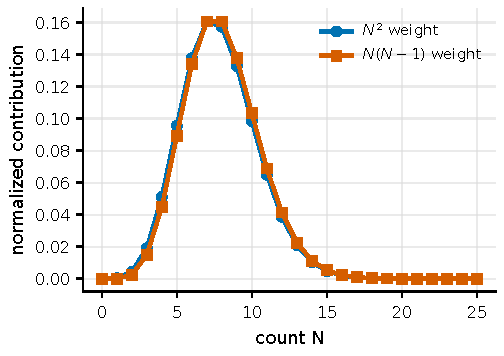
\includegraphics[width=0.86\linewidth]{figures/generated/chapter_04/ch04_factorial_moments.pdf}
\caption{The ordinary second moment \(N^2\) and the factorial moment \(N(N-1)\) weight different photon numbers \(N\) differently. Coincidence detection concerns only ordered pairs formed of \emph{different} photons, so normal ordering automatically subtracts the spurious contribution \(N^2-N(N-1)=N\) of ``the same photon paired with itself.'' This is exactly why what appears in second-order photon statistics is \(\langle N(N-1)\rangle\), not \(\langle N^2\rangle\).}
\label{fig:e07-factorial-moments}
\end{figure}

\section{Slicing the Event Table into Time Gates: Mean, Variance, and the Mandel Parameter}
\label{sec:e07-time-gate}

The previous section discussed ``instantaneous'' operator expectations. But what a real telescope hands back is a time-stamped event table: a long string of records of ``some photon arriving at some moment'' (the structure, clock, dead time, and other hardware details of this table are left for Chapter~\ref{chap:e13}). To turn an operator expectation like \eqref{eq:e07-b2-from-clicks} into a number that can truly be computed from data, we need a concrete operation: \textbf{slice continuous time into ``time gates'' (bins) each of width \(\Delta t\), and count how many photons fall into each.}

Let the count in the \(k\)th time gate be \(N_k\) (a dimensionless integer). Collecting the counts of many gates gives a counting distribution \(P(N)\): what fraction of time gates have \(N\) photons. For this distribution, we care about the two most basic statistics, the mean and the variance:

\begin{equation}
  \bar N=\langle N\rangle=\sum_{N=0}^{\infty}N\,P(N),
  \qquad
  \sigma_N^2=\big\langle N^2\big\rangle-\bar N^{\,2}
  =\sum_{N=0}^{\infty}(N-\bar N)^2\,P(N).
  \label{eq:e07-mean-var}
\end{equation}
\begin{formulaexplain}
\(\bar N\) is the \emph{mean} count per time gate, and \(\sigma_N^2\) is the size of the \emph{fluctuation} of the count between gates (the variance). The mean tells you ``how bright on average,'' the variance tells you ``how much it flickers.'' Judging the quantumness of light looks at the latter relative to the former.
\end{formulaexplain}

Let us account for each: \(\bar N\) is dimensionless, the mean photon number within the gate width \(\Delta t\), equal to the count rate \(r\) (units \(\mathrm{s^{-1}}\)) times the gate width, \(\bar N=r\,\Delta t\). \(\sigma_N^2\) is also dimensionless, the average of the squared deviation of the count from the mean. Here one must remember something very counterintuitive in astronomy: the gate width \(\Delta t\) is usually chosen very small, say \(\Delta t=1\,\mathrm{ns}\), while the count rate of a visible-light point source may be only \(r=10^6\,\mathrm{s^{-1}}\), so

\[
  \bar N=r\,\Delta t=(10^6\,\mathrm{s^{-1}})(10^{-9}\,\mathrm{s})=10^{-3}.
\]

That is, \emph{only about one in a thousand time gates holds a photon}, the vast majority of gates are empty (\(N=0\)), occasionally a gate has \(N=1\), and the chance of two photons in the same gate is as small as \(\sim10^{-6}\). Intensity-correlation signals are never read out from a ``light-curve fluctuation'' visible to the naked eye, but are accumulated bit by bit from the tiny statistical deviations of \(10^8\) or \(10^{12}\) time gates. This is also why we must use statistics, not the eye, to judge the properties of light.

\paragraph{Taking Poisson as the zero point: Mandel Q}
\label{sec:e07-mandel-q}

Now we need a ruler to measure ``whether this beam of light clusters more than random arrival, or is more orderly.'' The natural zero point is the \textbf{Poisson distribution}: if photons each come on their own, mutually independent (a coherent state is exactly so, see Chapter~\ref{chap:e06}), the count follows Poisson statistics, which has a signature property, the \emph{variance is exactly equal to the mean}:
\[
  \text{Poisson:}\quad \sigma_N^2=\bar N .
\]
(We computed this directly from \(P(N)=e^{-\bar N}\bar N^N/N!\) in Chapter~\ref{chap:e06}; it is the definition of shot noise.) Taking this as the zero point, Mandel uses a dimensionless number, the \textbf{Mandel parameter} (Mandel \(Q\) parameter), to measure the deviation:

\begin{equation}
  Q\equiv\frac{\sigma_N^2-\bar N}{\bar N}.
  \label{eq:e07-mandel-q}
\end{equation}
\begin{formulaexplain}
\(Q\) sets the Poisson \(\sigma_N^2=\bar N\) as the zero point and measures ``by what fraction the variance exceeds (or falls short of) the mean.'' \(Q=0\) Poisson (coherent state), \(Q>0\) super-Poisson, photons cluster (thermal light), \(Q<0\) sub-Poisson, photons overly regular (can only be non-classical light).
\end{formulaexplain}

Read term by term. The numerator \(\sigma_N^2-\bar N\) is ``the part by which the variance exceeds Poisson,'' and the denominator \(\bar N\) makes it dimensionless. Three cases, three physics:

\begin{itemize}
  \item \textbf{\(Q=0\) (Poissonian)}: the variance exactly equals the mean. Photons arrive independently at random, with no extra clustering and no extra regularity. An ideal stable laser, a coherent state, is here.
  \item \textbf{\(Q>0\) (super-Poissonian)}: the variance is larger than the mean. Photons tend to arrive \emph{in groups}: some stretch of time has excess intensity and multiple photons crowd in; another stretch is low and they thin out together. This is the signature of thermal light and chaotic light, and the source of HBT bunching.
  \item \textbf{\(Q<0\) (sub-Poissonian)}: the variance is \emph{smaller} than the mean, the count more ``regular,'' more evenly spaced than the random case. This cannot be explained by any positive classical intensity fluctuation and is a genuine non-classical signal (single-photon source, resonance fluorescence). Note \(Q\) has a lower bound: because \(N\ge0\), one can prove \(Q\ge-1\), with \(Q=-1\) corresponding to an ideal number state with completely fixed photon number in every gate.
\end{itemize}

An order-of-magnitude example. The count of single-mode thermal light within gate width \(\Delta t\) follows the Bose--Einstein distribution, with variance \(\sigma_N^2=\bar N+\bar N^2\) (Chapter~\ref{chap:e06}). Substituting into \eqref{eq:e07-mandel-q}:
\[
  Q_{\rm th}=\frac{(\bar N+\bar N^2)-\bar N}{\bar N}=\bar N .
\]
The \(Q\) of ideal single-mode thermal light equals its own mean count, which sounds substantial, but do not forget that in the visible few-photon-per-mode limit \(\bar n_\nu\sim10^{-2}\) (Chapter~\ref{chap:e05}), so even for pure single-mode thermal light, \(Q\) itself is only a few percent. Real multi-mode observation presses it even lower, which is precisely the theme of the next section.

\section{From Mandel Q to g(2)(0): An Algebraic Identity}
\label{sec:e07-q-to-g2}

We now have two languages: one is the language of ``photons arriving in pairs,'' whose protagonist is \(g^{(2)}(0)=\langle N(N-1)\rangle/\bar N^2\) (which is the time-gate version of the previous chapter's \(b_2\), and also the value of the second-order coherence function of Chapter~\ref{chap:e08} at zero delay); the other is the language of ``count variance,'' whose protagonist is the Mandel \(Q\). These two say the same thing, and what \emph{precisely} connects them is only a piece of middle-school algebra.

The key step is to express the factorial moment \(\langle N(N-1)\rangle\) in terms of the mean and the variance. Expand \(N(N-1)=N^2-N\), and average both sides:
\[
  \big\langle N(N-1)\big\rangle=\big\langle N^2\big\rangle-\langle N\rangle
  =\big\langle N^2\big\rangle-\bar N .
\]
Then use the definition of the variance \(\sigma_N^2=\langle N^2\rangle-\bar N^2\), that is, \(\langle N^2\rangle=\sigma_N^2+\bar N^2\), substituting in:
\begin{equation}
  \big\langle N(N-1)\big\rangle=\sigma_N^2+\bar N^{\,2}-\bar N .
  \label{eq:e07-identity}
\end{equation}
\begin{formulaexplain}
A purely algebraic identity: factorial moment = variance + mean squared \(-\) mean. It converts the \(\langle N(N-1)\rangle\) of the ``pair language'' into the \(\sigma_N^2\) and \(\bar N\) of the ``variance language,'' and is the sole bridge connecting \(g^{(2)}(0)\) and \(Q\).
\end{formulaexplain}

There is no physical approximation here; it is purely a matter of splitting \(N(N-1)\) open and rearranging, and it holds for \emph{any} counting distribution. Now substitute it into the definition of \(g^{(2)}(0)\). Dividing by \(\bar N^2\):
\[
  g^{(2)}(0)=\frac{\langle N(N-1)\rangle}{\bar N^{\,2}}
  =\frac{\sigma_N^2+\bar N^{\,2}-\bar N}{\bar N^{\,2}}
  =\underbrace{\frac{\bar N^{\,2}}{\bar N^{\,2}}}_{=1}
  +\frac{\sigma_N^2-\bar N}{\bar N^{\,2}} .
\]
Take one look at the numerator and denominator of the last term: \(\sigma_N^2-\bar N\) is exactly the numerator of the Mandel \(Q\), and \(Q=(\sigma_N^2-\bar N)/\bar N\), so \((\sigma_N^2-\bar N)/\bar N^2=Q/\bar N\). Thus
\begin{equation}
  g^{(2)}(0)=\frac{\langle N(N-1)\rangle}{\bar N^{\,2}}
  =1+\frac{Q}{\bar N}.
  \label{eq:e07-g2-q}
\end{equation}
\begin{formulaexplain}
The zero-delay second-order coherence \(g^{(2)}(0)\) and the Mandel \(Q\) differ only by a \(\bar N\). \(Q\) measures the absolute variance excess, \(g^{(2)}(0)\) measures the normalized pairing excess; the smaller the mean count \(\bar N\), the larger a \(g^{(2)}(0)-1\) the same \(Q\) levers up.
\end{formulaexplain}

Let us account term by term: \(g^{(2)}(0)\) is dimensionless, \(=1\) the independent-arrival baseline, \(>1\) bunching, \(<1\) antibunching. \(Q\) is dimensionless, \(\bar N\) is dimensionless. Equation \eqref{eq:e07-g2-q} is the most practical conversion of this chapter: it locks the ``variance language'' and the ``pair language'' together. Use it to check self-consistency: single-mode thermal light \(Q_{\rm th}=\bar N\), substituting gives \(g^{(2)}(0)=1+\bar N/\bar N=2\), exactly the thermal bunching peak of Chapter~\ref{chap:e06}; coherent state \(Q=0\), giving \(g^{(2)}(0)=1\), the Poisson baseline. Both ends check out.

Equation \eqref{eq:e07-g2-q} also hides a key lesson for astronomical observation, which Figure~\ref{fig:e07-mandel-q-g2} draws out: \(\bar N\) is in the denominator. When the mean count is very low (the weak-light limit), even a very small \(Q\) can correspond to a \(g^{(2)}(0)\) markedly deviating from 1; conversely, widening the time gate makes \(\bar N\) larger and also averages many mutually incoherent time modes into the same \(N\), both together diluting away \(g^{(2)}(0)-1\). So there is an iron rule that must be written into any intensity-correlation report:

\begin{quote}
\textbf{Reporting only \(g^{(2)}(0)\) or only \(Q\) is incomplete.} One must simultaneously give four things: \(Q\) (or \(g^{(2)}(0)-1\)), the \textbf{time gate width \(\Delta t\)}, the \textbf{effective mode count \(M\)}, and the \textbf{mean count \(\bar N\)}. Miss any one, and others cannot judge whether what you measured is an intrinsic signal or a residual shadow after gate-width dilution.
\end{quote}

\begin{figure}[tbp]
\centering
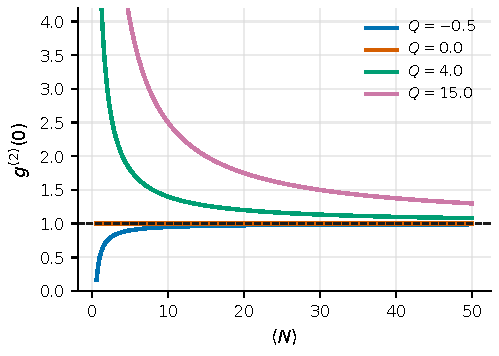
\includegraphics[width=0.86\linewidth]{figures/generated/chapter_04/ch04_mandel_q_g2.pdf}
\caption{Within a fixed time gate, the Mandel \(Q\) determines the zero-delay second-order coherence through \(g^{(2)}(0)=1+Q/\bar N\). The lower the mean count \(\bar N\), the larger the \(g^{(2)}(0)-1\) that the same \(Q\) levers up; widening the time gate or averaging more modes makes \(\bar N\) grow and \(Q\) be diluted, and the curve gradually falls back to the Poisson baseline 1. This explains why, when reporting second-order correlations, one must simultaneously note the gate width, the mode count, and the mean count.}
\label{fig:e07-mandel-q-g2}
\end{figure}

\section{Multi-Mode Dilution: Why the Astronomical Excess Is a Small Number, Not 1}
\label{sec:e07-multimode}

In the textbooks, the bunching peak of single-mode thermal light is a proud \(g^{(2)}(0)=2\), that is, an excess \(g^{(2)}(0)-1=1\). But open any real astronomical intensity-interferometry paper and the peak height you see is a humble small number like \(10^{-3}\) or \(10^{-6}\). Is the signal lost? No. It has been diluted by \emph{multi-mode averaging}. This section works out the dilution.

Recall Chapter~\ref{chap:e05}: in astronomy ``one channel'' is almost never a single quantum mode, but a sum of \(M\) independent modes, \(M\simeq(\Delta t/\tau_c)(A\Omega/\lambda^2)N_{\rm pol}\), readily thousands upon thousands in the visible. Now let us work out the statistical consequence of this sentence.

Let the detected total count \(N\) be the sum of the contributions of \(M\) \emph{independent, similar-intensity} thermal-light modes, each with mean count \(m=\bar N/M\). For a single thermal mode, the variance is \(m+m^2\) (Bose--Einstein, Chapter~\ref{chap:e06}). When independent random variables are added, \textbf{the means add and the variances also add} (this is the standard conclusion in probability theory that the variance of independent variables is additive, which we cite directly). So the total variance is
\[
  \sigma_N^2=\sum_{i=1}^{M}(m+m^2)=M m+M m^2
  =\underbrace{Mm}_{=\bar N}+M\Big(\frac{\bar N}{M}\Big)^2 .
\]
The first term \(Mm=\bar N\) is the total mean (the shot-noise part), and the second term simplifies to \(M\cdot\bar N^2/M^2=\bar N^2/M\). Thus
\begin{equation}
  \sigma_N^2=\bar N+\frac{\bar N^{\,2}}{M}.
  \label{eq:e07-multimode-var}
\end{equation}
\begin{formulaexplain}
After averaging \(M\) independent thermal modes, the two parts of the variance: \(\bar N\) is the unavoidable shot noise, and \(\bar N^2/M\) is the extra ``fluctuation noise'' of thermal light. The more modes (the larger \(M\)), the thinner the second term is spread, and the more the light looks like Poisson.
\end{formulaexplain}

Let us account term by term: \(\bar N\) is the total mean count (dimensionless), \(M\) the effective mode count (dimensionless, \(\ge1\)), and \(\bar N^2/M\) the super-Poisson fluctuation remaining after dilution by \(M\). Now stuff \eqref{eq:e07-multimode-var} into the Mandel \(Q\) and \(g^{(2)}(0)\). First compute \(Q\):
\[
  Q=\frac{\sigma_N^2-\bar N}{\bar N}
  =\frac{\bar N^2/M}{\bar N}=\frac{\bar N}{M}.
\]
Then use the conversion \eqref{eq:e07-g2-q}:
\begin{equation}
  g^{(2)}(0)=1+\frac{Q}{\bar N}=1+\frac{1}{M}.
  \label{eq:e07-multimode-g2}
\end{equation}
\begin{formulaexplain}
After averaging \(M\) independent thermal modes, the bunching peak height drops from the single-mode \(g^{(2)}(0)-1=1\) to \(1/M\). This \(1/M\) law is the root of why the excess is always a small number in astronomical intensity interferometry.
\end{formulaexplain}

This \(g^{(2)}(0)=1+1/M\) is astonishingly clean, and the physics is clear too: the intensity fluctuations of \(M\) independent modes are each random and cancel one another, and on average the intensity grows steadier and steadier, so the ``clustering'' effect of bunching is thinned by a factor of \(M\). \(M=1\) gives the classical 2; \(M=1000\) gives \(1+10^{-3}\); \(M=10^6\) gives \(1+10^{-6}\). This is why what is directly read off an astronomical HBT plot is never the majestic 2, but a small-number excess that must be dug out from a vast number of event pairs.

Where do those \(M\) come from? Count them one by one (all within the mode-counting framework of Chapter~\ref{chap:e05}):

\begin{itemize}
  \item \textbf{Polarization (2 modes)}: if the polarization is not projected onto a single channel, the two orthogonal polarizations are each an independent thermal mode, \(M_{\rm pol}\simeq2\), immediately pressing the ideal peak from 2 down to 1.5.
  \item \textbf{Spatial speckle}: an image smeared by atmospheric jitter (seeing), or coupled into a thick fiber, or falling on a large pixel, takes in many spatial modes at once, \(M_{\rm sp}=A\Omega/\lambda^2\) can be very large.
  \item \textbf{Broadband multi-frequency modes}: the wider the filter, the more independent frequency modes within the bandwidth \(\Delta\nu\).
  \item \textbf{Gate width \(>\) coherence time}: this is the fiercest term. The visible-light coherence time \(\tau_c\sim1\,\mathrm{ps}\), while the fastest detector time response is \(\sim100\,\mathrm{ps}\)--\(1\,\mathrm{ns}\), so one time gate has packed in \(\Delta t/\tau_c\sim10^2\)--\(10^3\) independent time modes, and this term alone presses the excess down two or three orders of magnitude.
\end{itemize}

Substitute a set of real scales (taken from stellar thermal-light bunching experiments): central wavelength about \(7800\,\text{\AA}\), narrowest filter \(10\,\text{\AA}\), corresponding to \(\Delta\nu\simeq5\times10^{11}\,\mathrm{Hz}\) and coherence time \(\tau_c\simeq1.6\)--\(2\,\mathrm{ps}\); APD single-photon time jitter about \(500\,\mathrm{ps}\), and the relative response peak width of the two detectors about \(700\,\mathrm{ps}\). The ``gate width/coherence time'' term alone contributes \(M\sim700\,\mathrm{ps}/2\,\mathrm{ps}\sim350\)-fold dilution, and adding polarization and spatial modes, the ideal \(g^{(2)}(0)=2\) is pressed down to the observed peak \(g^{(2)}(0)-1\sim10^{-3}\) order, and experiments on three bright stars measured exactly this \(10^{-3}\)-order bunching peak \citep{2017MNRAS.472.4126G}. So to stress it once more: the \(1+10^{-3}\), \(1+10^{-6}\) appearing on a telescope correlation plot are not ``no bunching,'' but ``bunching diluted by \(M\).'' Only by dividing \(M\) cleanly out of the data can one recover the physics of the source itself. This dilution accounting will be used repeatedly in the Siegert relation of Chapter~\ref{chap:e08} and the spatial intensity interferometry of Chapter~\ref{chap:e10}.

\section{Detectors Are Not Ideal: Efficiency, Background, and Dead Time}
\label{sec:e07-nonideal}

Up to now we have pretended the detector is perfect: every arriving photon is counted, there is no noise, and the moment counting finishes the next can be counted. Real detectors satisfy none of these three. This section gives one sentence of physics for each of three non-idealities, and fortunately two of them can reuse the language we have already built, while the third leaves a hook for Chapter~\ref{chap:e13}. Figure~\ref{fig:e07-detection-loss} draws the two main threads of efficiency loss and background dilution together.

\paragraph{Efficiency η: loss is like a beamsplitter}
\label{sec:e07-efficiency}

A real detector has quantum efficiency \(\eta<1\): on average, only one in every \(1/\eta\) arriving photons is counted. How to model this? There is a beautiful and accurate picture: \textbf{loss is completely equivalent to inserting a beamsplitter of transmittance \(\eta\) in the light path}, the transmitted fraction \(\eta\) is counted, the reflected \(1-\eta\) is lost, and the other input port of the beamsplitter leaks in vacuum fluctuation.

The power of this picture is that it turns ``loss'' into ``each photon survives independently with probability \(\eta\),'' which in probability theory is called \textbf{binomial thinning}. And thinning a distribution has a key property: it is closed for the \emph{Poisson} distribution (Poisson thinned is still Poisson), and it \emph{pulls toward Poisson} for a super-Poisson distribution.

Let us work this out fully and see how the Mandel \(Q\) changes. Let the number of photons \emph{arriving} in some time gate be the random variable \(N\) (mean \(\bar N\), variance \(\sigma_N^2\)), and the number \emph{counted} be \(M\). Binomial thinning means: given \(N\), each photon survives independently with probability \(\eta\), so the conditional distribution is binomial \(M\mid N\sim\mathrm{Binomial}(N,\eta)\), whose conditional mean and conditional variance are the standard results of the binomial distribution
\[
  \mathbb E[M\mid N]=\eta N,\qquad
  \operatorname{Var}(M\mid N)=N\,\eta(1-\eta).
\]
The mean is obtained by taking the expectation directly: \(\bar M=\mathbb E[\eta N]=\eta\bar N\). The variance requires the \textbf{law of total variance} \(\operatorname{Var}(M)=\mathbb E[\operatorname{Var}(M\mid N)]+\operatorname{Var}(\mathbb E[M\mid N])\): it splits the total fluctuation into ``the binomial jitter within each \(N\)'' and ``the fluctuation of \(N\) itself between gates,'' and is the standard tool for handling this kind of two-layer randomness of ``random survival within a random number.'' Substituting term by term:
\[
  \sigma_M^2
  =\underbrace{\mathbb E\big[N\,\eta(1-\eta)\big]}_{=\,\eta(1-\eta)\bar N}
  +\underbrace{\operatorname{Var}(\eta N)}_{=\,\eta^2\sigma_N^2}
  =\eta(1-\eta)\bar N+\eta^2\sigma_N^2 .
\]
The first term is the binomial shot noise introduced by loss itself, and the second is the residual of the original fluctuation shrunk by \(\eta^2\). Stuff \(\bar M=\eta\bar N\) and this \(\sigma_M^2\) together into the definition of the Mandel parameter \eqref{eq:e07-mandel-q}:
\[
  Q_M=\frac{\sigma_M^2-\bar M}{\bar M}
  =\frac{\eta(1-\eta)\bar N+\eta^2\sigma_N^2-\eta\bar N}{\eta\bar N}
  =\frac{\eta^2\sigma_N^2-\eta^2\bar N}{\eta\bar N}
  =\eta\,\frac{\sigma_N^2-\bar N}{\bar N}=\eta\,Q .
\]
The middle step used \(\eta(1-\eta)\bar N-\eta\bar N=-\eta^2\bar N\), merging the two shot-noise terms and leaving exactly an overall factor of \(\eta\) to pull out. So thinning shrinks both the mean and the variance excess proportionally, \(\bar N\to\eta\bar N\), while
\[
  Q\ \longrightarrow\ \eta\,Q .
\]
One sentence of physics:

\begin{quote}
\textbf{Loss randomly deletes photons, dragging super-Poisson statistics toward the Poisson zero point.} As \(\eta\to0\), the count of any light degenerates to Poisson; this is also why very-low-efficiency detection ``erases'' quantum features.
\end{quote}

But here is a life-saving detail, to be firmly remembered: the \emph{normalized} \(g^{(2)}(0)\) is \textbf{immune} to loss. Because \(Q\to\eta Q\) while \(\bar N\to\eta\bar N\), substituting into \eqref{eq:e07-g2-q}:
\[
  g^{(2)}(0)=1+\frac{\eta Q}{\eta\bar N}=1+\frac{Q}{\bar N}\quad(\text{unchanged}).
\]
The \(\eta\) in the numerator and denominator cancels exactly. Physically this is very reasonable: loss merely deletes some photons at random and does not change the \emph{tendency} of the remaining photons to arrive in pairs. This is precisely the fundamental reason why intensity interferometry remains feasible even under astronomical conditions of low efficiency and scarce photons: \(g^{(2)}(0)-1\), the quantity we truly want to measure, does not fear loss. Loss hurts the \emph{signal-to-noise ratio} (fewer photons means fewer event pairs and larger statistical error), not the \emph{value} of the signal.

\paragraph{Background dilution: source photons are only a fraction}
\label{sec:e07-background}

The second non-ideality is background light: sky glow, moonlight, dark counts, neighboring objects, all contribute source-unrelated counts in the same channel. Let the source photons make up a fraction \(f\) of the total count (source fraction, \(0<f\le1\)), the remaining \(1-f\) being uncorrelated background. The background itself carries no bunching peak (it is independently Poisson), and one two-photon coincidence requires \emph{both} photons to come from the source, each carrying a factor \(f\). So the measured excess is pressed down by \(f^2\):
\begin{equation}
  g^{(2)}_{\rm obs}(0)-1\simeq f^2\big[g^{(2)}_{\rm src}(0)-1\big].
  \label{eq:e07-background}
\end{equation}
\begin{formulaexplain}
The background dilutes the source signal by \(f^2\): both clicks must be source photons to count, each contributing a factor \(f\). When the source is only half (\(f=0.5\)), the bunching peak drops to one quarter of the original.
\end{formulaexplain}

Let us account term by term: \(f\) is the fraction of source counts in the total count (dimensionless), \(g^{(2)}_{\rm src}(0)\) is the second-order coherence of the source itself, and \(g^{(2)}_{\rm obs}(0)\) is what is measured after the background is mixed in. This \(f^2\) law and the \(1/M\) of multi-mode dilution are two parallel gates: one comes from ``how many unrelated modes are mixed into the channel,'' the other from ``how much unrelated background is mixed into the count.'' When doing an error budget (Chapter~\ref{chap:e15} will develop this systematically), both must be honestly multiplied in.

\paragraph{Dead time and afterpulsing: left for Chapter 13}
\label{sec:e07-deadtime}

The third non-ideality is that after counting one photon, the detector has a short \emph{dead time} during which it cannot respond again (single-photon detectors often have \(10\)--\(100\,\mathrm{ns}\)), plus the spurious counts that occasionally appear after a trigger (afterpulsing). These two dig holes and make false peaks in the autocorrelation \emph{near zero delay}, contaminating exactly the place we most want to look. They do not change the basic rule of ``counting \(n(n-1)\)'' of this chapter, but they distort the measured correlation peak shape and require dedicated hardware countermeasures (the most common being to split the light with a beamsplitter onto two independent detectors for cross-correlation, bypassing the dead time of a single detector). These belong to the hardware details of detectors and event tables, and we leave them for dedicated treatment in Chapter~\ref{chap:e13}, mentioning them here in just one sentence and setting them aside.

\begin{figure}[tbp]
\centering
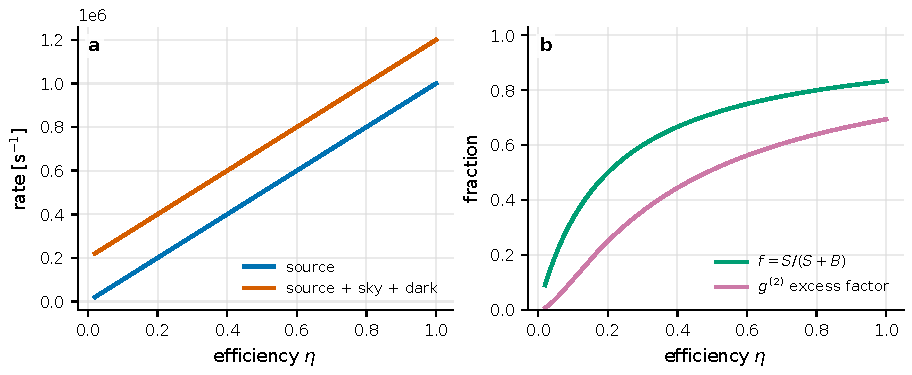
\includegraphics[width=0.85\linewidth]{figures/generated/chapter_03/ch03_detection_loss_background.pdf}
\caption{Two non-ideal effects that pull the observed statistics toward the Poisson baseline. Efficiency loss \(\eta\) is equivalent to the binomial thinning of a beamsplitter, randomly deleting photons and pressing the Mandel \(Q\) toward the zero point as \(Q\to\eta Q\) (but the normalized \(g^{(2)}(0)\) is unchanged); background dilution presses the source signal down by the square \(f^2\) of the source-photon fraction \(f\). Together with the multi-mode dilution \(1/M\), the two form the three gates by which astronomical intensity-correlation signals are pressed into a small-number excess.}
\label{fig:e07-detection-loss}
\end{figure}

\section{Chapter Summary}
\label{sec:e07-summary}

\begin{itemize}
  \item \textbf{Detection is absorption, so what is counted is normal-ordered.} The single-click rate \(\propto\langle\hat a^\dagger\hat a\rangle=\langle\hat n\rangle\); the two-coincident-click rate \(\propto\langle\hat a^\dagger\hat a^\dagger\hat a\hat a\rangle=\langle\hat n(\hat n-1)\rangle\). Using \([\hat a,\hat a^\dagger]=1\) one can prove exactly that \(\hat a^\dagger\hat a^\dagger\hat a\hat a=\hat n(\hat n-1)\).
  \item \textbf{\(n(n-1)\) rather than \(n^2\), because self-pairing is subtracted.} One START and one STOP must come from two \emph{different} absorptions; the \(N\) spurious pairs of ``the same photon paired with itself'' in \(N^2\) are automatically subtracted by normal ordering, leaving \(N(N-1)\) true pairs, precisely the origin of the \(b_2\) numerator of Chapter~\ref{chap:e06}.
  \item \textbf{Time gate + Mandel \(Q\).} Slice the event table into gates of width \(\Delta t\), count \(N\), obtain \(\bar N=r\Delta t\) and \(\sigma_N^2\); \(Q=(\sigma_N^2-\bar N)/\bar N\) takes Poisson as the zero point: \(Q=0\) Poisson, \(Q>0\) super-Poisson (thermal light), \(Q<0\) sub-Poisson (non-classical).
  \item \textbf{One identity connects the two languages.} From \(\langle N(N-1)\rangle=\sigma_N^2+\bar N^2-\bar N\) one derives \(g^{(2)}(0)=1+Q/\bar N\). When reporting, one must simultaneously give \(Q\), the gate width \(\Delta t\), the mode count \(M\), and the mean count \(\bar N\); none may be missing.
  \item \textbf{The \(1/M\) law of multi-mode dilution.} After averaging \(M\) independent thermal modes, \(\sigma_N^2=\bar N+\bar N^2/M\) and \(g^{(2)}(0)=1+1/M\). Polarization (2), spatial speckle, broadband multi-frequency modes, and gate width \(>\tau_c\) all contribute to \(M\), which is why the astronomical excess is often \(10^{-3}\) or \(10^{-6}\) rather than 1.
  \item \textbf{Detector non-idealities.} Efficiency \(\eta\) acts like a beamsplitter, binomial thinning pressing \(Q\to\eta Q\) (super-Poisson dragged toward Poisson), but the normalized \(g^{(2)}(0)\) unchanged; the background presses the signal down by \(f^2\); dead time/afterpulsing are left for Chapter~\ref{chap:e13}.
\end{itemize}

\medskip
\noindent\textbf{Questions to Ponder.}
\begin{enumerate}
  \item A beam of single-mode thermal light is measured to have \(g^{(2)}(0)=2\). If you widen the time gate from \(1\,\mathrm{ps}\) to \(1\,\mathrm{ns}\) (the coherence time still being \(1\,\mathrm{ps}\)), how many effective time modes does it become? To roughly what does \(g^{(2)}(0)-1\) then drop?
  \item If the detection efficiency \(\eta\) drops from \(0.5\) to \(0.05\), will the measured \(g^{(2)}(0)-1\) change? Will the Mandel \(Q\) change? Explain why for each.
  \item In an observation the source photons make up only \(f=1/3\) of the total count, the rest being sky-glow background. If the source itself is single-mode thermal light (\(g^{(2)}_{\rm src}(0)=2\)), roughly what \(g^{(2)}_{\rm obs}(0)\) do you measure in this channel?
\end{enumerate}

\chapter{\texorpdfstring{The Coherence Functions $g^{(1)}$, $g^{(2)}$ and the Siegert Relation}{The Coherence Functions g1, g2 and the Siegert Relation}}
\label{chap:e08}

\begin{chapteropening}
By now, what the telescope hands us is no longer "a blob of brightness" but the \textbf{event list} introduced in Chapter \ref{chap:e07}: a string of time-stamped "clicks." The question we now ask is no longer "how bright is it on average," but something far more subtle: \emph{do these clicks bear any relationship to one another?} If the photons in two detectors, in two time gates, arrive merely at random and independently, then their occasional simultaneous firing is pure coincidence; but if they fire together \emph{more often than chance}, or \emph{less often than chance}, then the event list hides the fingerprint of the light field's statistics. This chapter teaches you a language for translating "the event list" into "the statistics of the light field": first-order coherence \(g^{(1)}\) measures the phase memory of the electric field, while second-order coherence \(g^{(2)}\) measures the tendency of photons to arrive in pairs. What connects the two is the climax of this chapter: the Siegert relation. It reveals something close to magic: by counting nothing but the "degree of synchrony" of intensity fluctuations, you can read off the squared modulus of the field's degree of coherence. This is precisely what underwrites all of the intensity interferometry and imaging that follows.
\end{chapteropening}

\section{Why Give "Correlation" a Function of Its Own}
\label{sec:e08-why-correlation}

Let us first catch the conclusions of the previous stage. Chapter \ref{chap:e02} told us that light "remembers" its own phase only within a very short coherence time \(\tau_c\); in the broadband visible, \(\tau_c\) is as short as picoseconds, while detectors are as slow as hundreds of picoseconds or more, so a single time gate averages over hundreds or thousands of mutually incoherent wave trains. Chapter \ref{chap:e06} then told us that different states of light (coherent, thermal, number states) can share exactly the same mean brightness yet differ enormously in their photon-number \emph{fluctuations}. Put these two facts together and a natural thought arises: \emph{since the total intensity of a single exposure has erased so much information, could we stop looking at the "total" and instead look at the "echo between two detections"?}

This is exactly where the coherence function comes into its own. Its idea is extremely plain, and it descends directly from the autocorrelation function of Chapter \ref{chap:e02}: take the light field (or the photon stream) and compare it with "a copy of itself delayed by \(\tau\)," and see how alike they still are. The only difference lies in \emph{what} is compared:

\begin{itemize}
  \item If we compare the \textbf{amplitude and phase of the electric field}, we obtain first-order coherence \(g^{(1)}(\tau)\): it answers "how much phase does the field still remember after a delay \(\tau\)?" Amplitude interferometry (Chapter \ref{chap:e09}) uses precisely this.
  \item If we compare the \textbf{intensity (photon arrivals)}, we obtain second-order coherence \(g^{(2)}(\tau)\): it answers "are two detection events more likely to appear in pairs than the random case?" Hanbury Brown--Twiss (HBT) intensity interferometry uses precisely this \citep{1956Natur.177...27B}.
\end{itemize}

The reason we write "correlation" as \emph{a function of the delay \(\tau\)}, rather than a single number, is that the strength of the echo varies with delay: the echo is strongest at very small delay, and once the delay is stretched beyond the coherence time, the two detections lose all "contact." The \emph{height} and \emph{width} of this echo-versus-\(\tau\) decay curve encode, respectively, the kind of light (thermal or laser) and its spectral width (coherence time). This chapter will lay out both of these curves one by one, and then join them with a single bridge: the Siegert relation.

\section{First-Order Coherence: How Much Phase Does the Field Remember Across \texorpdfstring{$\tau$}{tau}}
\label{sec:e08-g1}

Let us begin with the easiest to picture, the first order. In Chapter \ref{chap:e05} we wrote the positive-frequency electric field on the detector surface as the operator \(\hat E^{(+)}(t)\) (which contains only the annihilation operator \(\hat a\), whose action is to "remove one photon"), and its Hermitian conjugate \(\hat E^{(-)}(t)\) (which contains only the creation operator \(\hat a^\dagger\)) is the negative-frequency part. The first-order coherence function is defined by "multiplying the fields at two instants and averaging":

\begin{equation}
  G^{(1)}(t_1,t_2)=\big\langle \hat E^{(-)}(t_1)\,\hat E^{(+)}(t_2)\big\rangle,
  \qquad
  g^{(1)}(\tau)=\frac{G^{(1)}(t,t+\tau)}{G^{(1)}(t,t)} .
  \label{eq:e08-g1}
\end{equation}
\begin{formulaexplain}
\(G^{(1)}\) is the first-order field correlation; \(\hat E^{(+)},\hat E^{(-)}\) are the positive- and negative-frequency field operators; \(\langle\cdot\rangle\) is the expectation over the quantum state; \(g^{(1)}\) is the normalized version obtained by dividing by the zero-delay value; \(\tau=t_2-t_1\) is the delay. It measures how much phase memory the field still retains across a delay \(\tau\).
\end{formulaexplain}

Let us pin down every symbol. \(G^{(1)}(t,t)=\langle\hat E^{(-)}(t)\hat E^{(+)}(t)\rangle\) is just the mean intensity at time \(t\) (a positive real number, carrying the dimensions of intensity), so after normalization \(g^{(1)}\) is a dimensionless complex number. If the light field is \emph{statistically stationary} (its statistical properties do not drift with absolute time, the normal condition for a stable source), the correlation depends only on the delay \(\tau\) and not on the starting point \(t\), so \(g^{(1)}\) becomes a function of \(\tau\) alone. Its modulus \(|g^{(1)}(\tau)|\) lies between \([0,1]\), and its physical meaning can be captured in a single sentence:

\begin{itemize}
  \item \(|g^{(1)}(\tau)|\to1\): the field after a delay \(\tau\) is still in step with the original field, its phase predictable: \textbf{coherent}. Superpose it with its pre-delay self and it will draw out sharp interference fringes.
  \item \(|g^{(1)}(\tau)|\to0\): the field has completely forgotten the phase it held \(\tau\) ago: \textbf{amnesia}. Superposition now gives a smeared-out, fringe-free brightness.
\end{itemize}

This is precisely the "field version" of the autocorrelation function \(\Gamma(\tau)\) of Chapter \ref{chap:e02}: the width over which \(g^{(1)}(\tau)\) decays from its peak of 1 down to 0 is the coherence time \(\tau_c\). And \(\tau_c\) is set by the spectral width; recall the two formulas of Chapter \ref{chap:e02}:

\begin{equation}
  \Delta\nu\simeq\frac{c\,\Delta\lambda}{\lambda^2},
  \qquad
  \tau_c\simeq\frac{1}{\Delta\nu}\simeq\frac{\lambda^2}{c\,\Delta\lambda}.
  \label{eq:e08-tauc}
\end{equation}
\begin{formulaexplain}
\(\Delta\nu\) is the frequency bandwidth (Hz), \(\Delta\lambda\) is the wavelength bandwidth, \(\lambda\) is the central wavelength, \(c\) is the speed of light, and \(\tau_c\) is the coherence time (s). It converts "how narrow the filter is" directly into "how long the field's phase memory lasts."
\end{formulaexplain}

Let us plug in real numbers to feel the magnitude. Take a "very narrow" filter: central wavelength \(\lambda=780\,{\rm nm}\), bandwidth \(\Delta\lambda=1\,{\rm nm}\). First compute the frequency bandwidth (in CGS, \(c=3\times10^{10}\,{\rm cm\,s^{-1}}\), \(\lambda=7.8\times10^{-5}\,{\rm cm}\), \(\Delta\lambda=10^{-7}\,{\rm cm}\)):
\[
  \Delta\nu\simeq\frac{(3\times10^{10})(10^{-7})}{(7.8\times10^{-5})^2}
  =\frac{3\times10^{3}}{6.1\times10^{-9}}
  \approx4.9\times10^{11}\,{\rm Hz},
\]
so
\[
  \tau_c\simeq\frac{1}{4.9\times10^{11}\,{\rm Hz}}\approx2\times10^{-12}\,{\rm s}=2\,{\rm ps}.
\]
That is to say, even through a 1-nanometer narrowband filter, the electric field of a star's thermal light remembers its own phase for only about 2 picoseconds before turning the page. This 2 ps will reappear again and again in this chapter, and it will directly set how narrow the later intensity-correlation peak is, and by how many factors it is diluted.

\section{Second-Order Coherence: Do Photons Like to Arrive in Pairs}
\label{sec:e08-g2}

Change the question from "does the field still remember the phase" to "are two detection events correlated," and we enter the second order. The definition given by the quantum theory of photodetection (Chapter \ref{chap:e07}) is the average of four field operators arranged in a particular order:

\begin{equation}
  G^{(2)}(t_1,t_2)=\big\langle
    \hat E^{(-)}(t_1)\,\hat E^{(-)}(t_2)\,\hat E^{(+)}(t_2)\,\hat E^{(+)}(t_1)
  \big\rangle,
  \qquad
  g^{(2)}(\tau)=\frac{G^{(2)}(t,t+\tau)}{G^{(1)}(t,t)\,G^{(1)}(t+\tau,t+\tau)} .
  \label{eq:e08-g2-field}
\end{equation}
\begin{formulaexplain}
\(G^{(2)}\) is the second-order field correlation; among the four operators, the two creation operators (\(\hat E^{(-)}\)) are all placed on the left and the two annihilation operators (\(\hat E^{(+)}\)) are all placed on the right: this is called \textbf{normal ordering}; as for the inner/outer nesting, it is paired by time (the \(t_1\) pair on the outermost layer, the \(t_2\) pair on the inner layer), guaranteeing the time order "absorb first at \(t_1\), then absorb at \(t_2\)." The denominator is the product of the mean intensities at the two instants; \(g^{(2)}\) is the normalized result. It measures whether photons tend to arrive in pairs.
\end{formulaexplain}

This formula deserves to be read slowly, term by term, because each term corresponds to something countable in the event list.

\textbf{Why this strange operator ordering?} Chapter \ref{chap:e07} explained that what a detector "counts" is the event of \emph{absorbing} a photon, and each absorption uses up one annihilation operator \(\hat E^{(+)}\). To detect one photon at each of the two instants \(t_1\) and \(t_2\), we apply two annihilation operators \(\hat E^{(+)}(t_2)\hat E^{(+)}(t_1)\) in succession to the state, obtaining the state vector \(\hat E^{(+)}(t_2)\hat E^{(+)}(t_1)|\psi\rangle\); the probability of this joint detection is exactly its squared modulus \(\big|\hat E^{(+)}(t_2)\hat E^{(+)}(t_1)|\psi\rangle\big|^2\), which upon expansion moves the two creation operators, unchanged, to the left. Thus the creation operators all sit on the left and the annihilation operators all on the right; this is normal ordering, and it guarantees that what we count are \emph{two distinct absorption events}, not the spurious term of a single photon pairing with itself. As for the "outer/inner" nesting in the formula, it comes purely from time pairing: the \(t_1\) pair (one creation, one annihilation) sits on the outermost layer, the \(t_2\) pair on the inner layer, locking in the temporal order "absorb first at \(t_1\), then absorb at \(t_2\)." This is a different matter from "creation on the left, annihilation on the right"; do not conflate them. This point was already foreshadowed in Chapter \ref{chap:e07}'s factorial moment \(\langle N(N-1)\rangle\): what the detector admits are ordered pairs made of distinct photons.

\textbf{What is the denominator?} The denominator \(G^{(1)}(t,t)\,G^{(1)}(t+\tau,t+\tau)=\langle I(t)\rangle\langle I(t+\tau)\rangle\) is the baseline of "how many accidental coincidences there should be if the two detections were completely independent." In other words, if the photons at the two instants are entirely uncorrelated, each arriving at random at its own mean rate, then the joint rate of their happening to be detected together is just the product of the two mean rates.

\textbf{What is the numerator?} The numerator is the true \emph{joint} detection intensity. Divide it by the "accidental-coincidence baseline of the independent case" and \(g^{(2)}\) becomes a dimensionless \emph{relative excess}:

\begin{itemize}
  \item \(g^{(2)}(\tau)=1\): the true coincidence exactly equals the random baseline, and photon arrivals are mutually independent. The ideal laser (coherent state, Chapter \ref{chap:e06}) is just like this: it gives Poisson counts, \(g^{(2)}=1\).
  \item \(g^{(2)}(0)>1\): near zero delay there are \emph{more} photon pairs than random, and photons like to cluster, called \textbf{bunching}. Ideal single-mode thermal light gives the beautiful value \(g^{(2)}(0)=2\).
  \item \(g^{(2)}(0)<1\): the zero-delay coincidence is \emph{suppressed}, and photons avoid one another, called \textbf{antibunching}. This cannot be explained by any positive-definite classical intensity fluctuation, and is the standard \emph{nonclassical} signature of single-photon sources and resonance fluorescence \citep{1977PhRvL..39..691K}.
\end{itemize}

Why is ideal single-mode thermal light exactly 2? The physical picture was already laid down in Chapter \ref{chap:e06}: the electric field of thermal light is the superposition of many small contributions with random phases, so the instantaneous intensity forms a random speckle of bright and dark patches; within a "bright patch" the detector is more likely to record several photons in succession, so coincidences rise near zero delay. And the specific number 2 is precisely the direct corollary of the next section's Siegert relation evaluated at \(\tau=0\); keep this suspense in mind for now.

In engineering estimates people often write the same thing in terms of continuous intensity:

\begin{equation}
  g^{(2)}(\tau)=\frac{\big\langle I(t)\,I(t+\tau)\big\rangle}{\big\langle I(t)\big\rangle^2}.
  \label{eq:e08-g2-classical}
\end{equation}
\begin{formulaexplain}
\(I(t)\) is the intensity (or the detector current or count rate proportional to it); the numerator is the joint fluctuation of the intensity at the two instants; the denominator is the square of the mean intensity (using stationarity, so the mean at the two instants is the same). This is the "classical form" of second-order coherence, convenient for estimation.
\end{formulaexplain}

This line is convenient, but it hides a \textbf{trap} that must be spelled out: which intensity is \(I(t)\), exactly? It could be the ideal \emph{instantaneous} intensity of the light field, or it could be the detector output current, the event rate recorded by the TDC, or the sampled ADC value. These two are worlds apart: the latter has already been \emph{convolved} by the detector's few-nanosecond response. If you plug into Eq.~\eqref{eq:e08-g2-classical} an \(I(t)\) that has been smeared by a 4 ns electronic response, what you get is the "post-response" \(g^{(2)}\), not the picosecond-wide correlation peak of the light field itself. Many astronomical intensity-correlation signals are not "unbunched"; rather, that peak, which should have risen to 2, has been suppressed by the finite time response, by multiple modes, and by background light down to \(10^{-3}\), \(10^{-6}\), or even smaller (Section \ref{sec:e08-telescope} will settle this account). So every time you write down Eq.~\eqref{eq:e08-g2-classical}, ask yourself one question: this \(I\), has it been convolved?

\section{The Siegert Relation: Reading the Squared Field Coherence from the Intensity Correlation}
\label{sec:e08-siegert}

Now we reach the climax of this chapter. The previous two sections each defined \(g^{(1)}\) (field phase memory) and \(g^{(2)}\) (photon pairing tendency), and they look like two entirely separate things: one about phase, one about intensity. The central miracle of the HBT experiment is this: for \textbf{Gaussian chaotic light} (that is, light such as thermal light, formed by the random superposition of a large number of independent small contributions), there exists an exact bridge between the two. Cross this bridge, and using only the measurement "count the intensity fluctuations" (something a detector can do) you can infer the field's degree of coherence, the phase information a detector "cannot see."

\paragraph{The Key Tool: the Gaussian Moment Theorem (Wick's Theorem)}
\label{sec:e08-gaussian-moment}

The pier of this bridge is a theorem from statistics, which we will first spell out on its own, never quietly substituting it in.

The electric field \(E(t)\) of thermal light is the random-phase superposition of a vast number of independent radiators (atoms, electrons). By the \textbf{central limit theorem} (the sum of a large number of independent random quantities tends toward a Gaussian distribution), the complex field \(E=E_r+iE_i\) approximately follows a \emph{zero-mean circularly symmetric complex Gaussian} distribution. The phrase "circularly symmetric" is crucial: it means the phase of the field is completely uniform over \([0,2\pi)\), from which we can deduce a property we will use immediately:

\begin{equation}
  \langle E(t_1)\,E(t_2)\rangle=0,
  \qquad\text{but}\qquad
  \langle E^*(t_1)\,E(t_2)\rangle=G^{(1)}(t_1,t_2)\neq0.
  \label{eq:e08-circular}
\end{equation}
\begin{formulaexplain}
The average of two fields multiplied together (neither starred) is zero, because their total phase is random and the positives and negatives cancel; only when one is starred and one is not does the phase cancel and a nonzero correlation survive. This is the defining property of a circularly symmetric Gaussian field.
\end{formulaexplain}

For such a field, the \textbf{Gaussian moment theorem} (called Isserlis's theorem in probability and Wick's theorem in quantum field theory) states: \emph{any higher-order moment can be decomposed into a sum of second-order moments (pairwise pairings), running over all ways of pairing}. And by Eq.~\eqref{eq:e08-circular}, only pairings of "one starred with one unstarred" are nonzero; all the rest vanish. This is all we will use: it is not an approximation, but a rigorous algebraic fact about the zero-mean circular Gaussian distribution.

\paragraph{Splitting the Fourth-Order Moment}
\label{sec:e08-factorize}

Now let us get to work. The numerator of the second-order coherence (written with classical intensity, \(I=E^*E\)) is a fourth-order moment:
\[
  \big\langle I(t)\,I(t+\tau)\big\rangle
  =\big\langle E^*(t)\,E(t)\,E^*(t+\tau)\,E(t+\tau)\big\rangle .
\]
Among the four fields, two are starred (\(E^*(t),E^*(t+\tau)\)) and two are unstarred (\(E(t),E(t+\tau)\)). By the Gaussian moment theorem, pair them two by two, keeping only the "starred with unstarred" terms. There are two legal pairings:

\emph{Pairing one}: \(E^*(t)\) with \(E(t)\), \(E^*(t+\tau)\) with \(E(t+\tau)\), each paired "in place." This gives
\[
  \langle E^*(t)E(t)\rangle\,\langle E^*(t+\tau)E(t+\tau)\rangle
  =\langle I(t)\rangle\,\langle I(t+\tau)\rangle=\langle I\rangle^2 .
\]

\emph{Pairing two}: \(E^*(t)\) with \(E(t+\tau)\), \(E^*(t+\tau)\) with \(E(t)\), a "cross" pairing. This gives
\[
  \langle E^*(t)E(t+\tau)\rangle\,\langle E^*(t+\tau)E(t)\rangle
  =G^{(1)}(\tau)\,G^{(1)}(-\tau)
  =G^{(1)}(\tau)\,\big[G^{(1)}(\tau)\big]^*
  =\big|G^{(1)}(\tau)\big|^2 .
\]
(Here we used the symmetry of a stationary field, \(G^{(1)}(-\tau)=[G^{(1)}(\tau)]^*\).) Adding the two terms:

\begin{equation}
  \big\langle I(t)\,I(t+\tau)\big\rangle=\langle I\rangle^2+\big|G^{(1)}(\tau)\big|^2 .
  \label{eq:e08-G2-factor}
\end{equation}
\begin{formulaexplain}
The left side is the measurable intensity correlation; on the right, the first term \(\langle I\rangle^2\) is the "random baseline of the independent case," and the second term \(|G^{(1)}(\tau)|^2\) is the extra fluctuation contributed by the field's degree of coherence. The fourth-order moment has thus been split into a sum of two second-order moments.
\end{formulaexplain}

Divide both sides by \(\langle I\rangle^2\), and noting that \(|g^{(1)}(\tau)|^2=|G^{(1)}(\tau)|^2/\langle I\rangle^2\), we immediately obtain the ideal form of the \textbf{Siegert relation}:
\[
  g^{(2)}(\tau)=1+\big|g^{(1)}(\tau)\big|^2 \qquad(\text{ideal single spatio-temporal-polarization mode}).
\]
At \(\tau=0\), \(|g^{(1)}(0)|=1\), so \(g^{(2)}(0)=1+1=2\). The suspense of the last section ("why is thermal light exactly 2") is now resolved: that 2 is the 1 of the random baseline, plus the 1 contributed when the field is fully coherent.

\paragraph{Installing It in a Real Telescope: the Visibility Factor \texorpdfstring{$\zeta$}{zeta}}
\label{sec:e08-zeta}

Real detection is never so ideal as "a single spatio-temporal-polarization mode." Unpolarized light mixes at least two polarizations, a broad spectrum has several frequency modes, atmospheric jitter (seeing, the phenomenon of a stellar image being blurred by turbulence) produces an image with several spatial speckles, and background light seeps in to dilute; all of these suppress that ideal 1. Bundle all these dilution factors into one \textbf{visibility factor} \(\zeta\), and the Siegert relation takes the signature form of this chapter:

\begin{equation}
  \boxed{\,g^{(2)}(\tau)=1+\zeta\,\big|g^{(1)}(\tau)\big|^2\,},
  \qquad 0<\zeta\le1 .
  \label{eq:e08-siegert}
\end{equation}
\begin{formulaexplain}
\(g^{(2)}-1\) is the excess of the intensity correlation; \(|g^{(1)}|^2\) is the squared modulus of the first-order field coherence; \(\zeta\) collects the dilution at the level of the \emph{true correlation} (mode number, polarization, background) and equals 1 for the ideal single mode. The finite time response is \emph{not} counted in \(\zeta\); it is handled separately by convolution in Section \ref{sec:e08-telescope}. This is the core bridge by which HBT reads the squared field coherence from the intensity correlation.
\end{formulaexplain}

Let us account for the sources of \(\zeta\) term by term: unpolarized thermal light already has \(M_{\rm pol}\simeq2\) polarization modes, which pulls the peak height from 2 down to 1.5 (i.e.\ \(\zeta\simeq1/2\)); multiple spatial speckles and multiple frequency modes each multiply by a further \(1/M\); and if the source photons account for fractions \(f_A,f_B\) of the total counts in the two channels (the rest being background), the correlation amplitude must be multiplied approximately by \(f_Af_B\). The product of these factors can easily push \(\zeta\) below \(10^{-3}\), which is why an astronomical HBT plot shows the decimal of \(g^{(2)}-1\), rather than the clean 1 of the textbook.

The significance of Eq.~\eqref{eq:e08-siegert} cannot be overstated: \emph{the left side is the intensity correlation that the event list can directly measure, while the \(g^{(1)}\) on the right is the field's degree of coherence}. And we have two independent routes to \(g^{(1)}\): it is the Fourier transform of the spectral line shape (the Wiener--Khinchin theorem, Chapter \ref{chap:e02}), and it is also the fringe visibility measured by an amplitude interferometer (Chapter \ref{chap:e09}). Thus the "degree of synchrony" of the intensity fluctuations is converted into the squared modulus of the field's degree of coherence.

\begin{figure}[tbp]
\centering
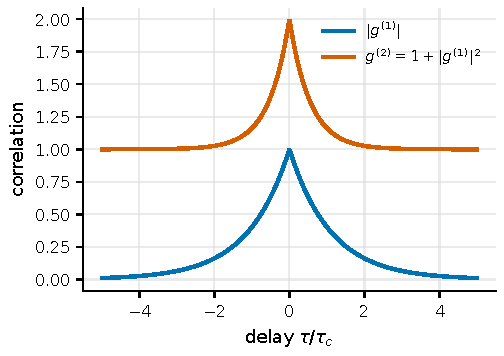
\includegraphics[width=0.86\linewidth]{figures/generated/chapter_04/ch04_siegert_relation.pdf}
\caption{The Siegert relation converts the decay of the first-order field coherence into the second-order intensity bunching peak. If \(|g^{(1)}(\tau)|\) decays with delay over the coherence time \(\tau_c\), then \(g^{(2)}(\tau)-1\) decays as \(|g^{(1)}(\tau)|^2\) and returns to the uncorrelated value 0 at large delay; the zero-delay peak height is 1 for the ideal single mode, and in real observations must be multiplied by the visibility factor \(\zeta\) (mode number, polarization, background; the finite time response is not included in \(\zeta\) but handled separately by convolution, see Section \ref{sec:e08-telescope}).}
\label{fig:e08-siegert}
\end{figure}

\paragraph{The Spectral Shape Sets the Peak Shape; the Coherent State Is the Exception}
\label{sec:e08-shapes}

Since \(g^{(1)}(\tau)\) is the Fourier transform of the spectral line, \emph{whatever the spectral line looks like, so looks the bunching peak}. Three common spectral shapes are worth remembering:

\begin{itemize}
  \item \textbf{Rectangular spectrum} (flat-topped within a bandwidth \(\Delta\nu\)): its Fourier transform is a sinc function, so \(|g^{(1)}(\tau)|^2\propto{\rm sinc}^2(\Delta\nu\,\tau)\), a peak with sidelobes.
  \item \textbf{Lorentzian spectrum} (as in collisional broadening or natural linewidth): \(|g^{(1)}(\tau)|=e^{-|\tau|/\tau_c}\) is a two-sided exponential decay, so \(g^{(2)}-1\propto e^{-2|\tau|/\tau_c}\), a sharp cusp.
  \item \textbf{Gaussian spectrum} (as in Doppler broadening): its Fourier transform is still a Gaussian, so \(|g^{(1)}(\tau)|^2\) is also Gaussian, a rounded dome.
\end{itemize}

Used in reverse, this becomes an experimental technique: measure the \emph{width} of the \(g^{(2)}(\tau)\) peak and you can infer the linewidth. For candidate astrophysical laser lines such as those near \(\eta\) Carinae, an ordinary spectrograph can hardly achieve a spectral resolving power \(R\equiv\lambda/\Delta\lambda\sim10^8\) (dimensionless), yet nanosecond-scale intensity correlation can place an independent constraint on linewidths from MHz to GHz \citep{2005NewA...10..361J,2008AIPC..984..216D,2014ApJ...789L..10T}.

But we must nail down the \textbf{boundary of validity}: the Siegert relation is \emph{exclusive to Gaussian chaotic light}. The ideal coherent state (laser) plainly has a long first-order coherence (\(g^{(1)}\) does not decay over long range), yet its \(g^{(2)}\equiv1\), never satisfying \(1+|g^{(1)}|^2\). The reason is exactly that the circular Gaussian assumption fails: a coherent state is not the superposition of a large number of random phases, and its field has no such bright-dark speckle fluctuation. Likewise, antibunched light, squeezed light, single-photon sources, strongly nonstationary pulses, and the superposition of a few coherent sub-sources all break Eq.~\eqref{eq:e08-siegert}. More common in astronomy is a mixed field: many non-thermal small sources that average to approximately thermal light, or a narrow non-thermal line superposed on a thermal continuum, so before using the Siegert relation, always confirm the "chaotic" pedigree of the light.

\section{From the Ideal Correlation to the Estimator in a Telescope}
\label{sec:e08-telescope}

The ideal \(g^{(2)}\) peak is both narrow and tall (picoseconds wide, peak height 1). But a detector is not infinitely fast; what it measures is the convolution of the ideal correlation with the \emph{instrument response}:

\begin{equation}
  g_{\rm obs}^{(2)}(\tau)-1=\int_{-\infty}^{+\infty}
  \big[g_{\rm true}^{(2)}(\tau')-1\big]\,R_{\Delta t}(\tau-\tau')\,{\rm d}\tau',
  \label{eq:e08-response-conv}
\end{equation}
\begin{formulaexplain}
\(g_{\rm true}^{(2)}\) is the intrinsic correlation of the light field; \(g_{\rm obs}^{(2)}\) is what is observed; \(R_{\Delta t}\) is the instrument response function with area normalized to 1 (jointly determined by detector jitter, electronic bandwidth, sampling window, and analysis bin); \(\tau'\) is the integration variable. Convolution broadens and lowers a narrow peak, but preserves its area.
\end{formulaexplain}

Here lies a fact easily misunderstood: convolution \emph{preserves area, not peak height}. A narrow peak of fixed area, smeared out by a much broader response, becomes shorter and fatter. If the intrinsic peak width \(\tau_c\) is much smaller than the effective response width \(\Delta t_{\rm eff}\), then the peak height is diluted approximately by the ratio \(\tau_c/\Delta t_{\rm eff}\). Combine this temporal dilution with the mode and background dilution of the previous section, and we obtain the \emph{error-budget formula} for the correlation peak height in a telescope:

\begin{equation}
  C_{\rm obs}\equiv g_{\rm obs}^{(2)}(0)-1
  \simeq C_{\rm true}\,\frac{\tau_c}{\Delta t_{\rm eff}}\,\frac{1}{M}\,f_A f_B,
  \label{eq:e08-contrast}
\end{equation}
\begin{formulaexplain}
\(C_{\rm obs}\) is the observed peak height, \(C_{\rm true}\) is the ideal peak height (1 for single-mode thermal light); \(\tau_c/\Delta t_{\rm eff}\) is the temporal dilution; \(M=M_{\rm pol}M_{\rm sp}\) is the number of polarization and spatial modes; \(f_A,f_B\) are the fractions of source photons out of the total counts in the two channels (background dilution). This is an order-of-magnitude formula; a precise analysis must put the measured response, the spectral shape \(|g^{(1)}|^2\), and the background together into the model.
\end{formulaexplain}

\begin{figure}[tbp]
\centering
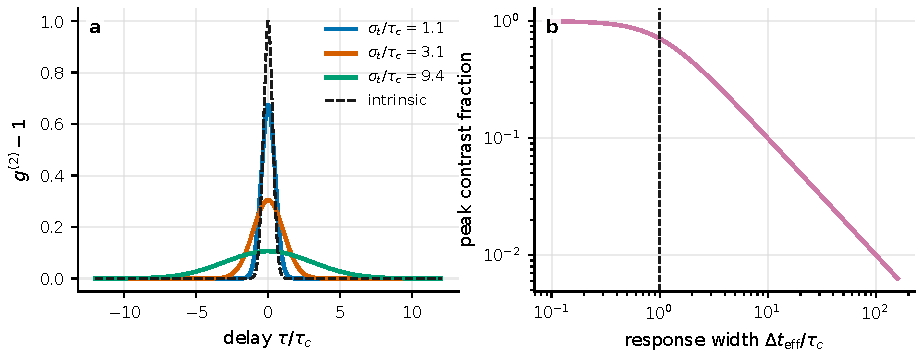
\includegraphics[width=0.95\linewidth]{figures/generated/chapter_04/ch04_response_convolution.pdf}
\caption{A finite time response broadens and lowers the narrow thermal-light bunching peak. Left: the dashed curve is the intrinsic picosecond-scale peak, and the solid curves are the observed peaks after convolution with different response widths; right: when \(\Delta t_{\rm eff}\gg\tau_c\), the zero-delay peak height falls approximately as \(\tau_c/\Delta t_{\rm eff}\): the area is preserved, but the peak height is diluted.}
\label{fig:e08-response}
\end{figure}

\textbf{Plugging in a real yardstick: Guerin's stellar bunching experiment.}\ Guerin et al.\ used a 1-meter telescope, a multimode fiber, a beam splitter, two avalanche photodiodes (APDs), and a delay histogram to measure the thermal-light bunching of a star \citep{2017MNRAS.472.4126G}. Their parameters make an excellent order-of-magnitude exercise: central wavelength about \(7800\,\text{\AA}\), narrowest filter bandwidth \(10\,\text{\AA}\). First compute the coherence time (as in Eq.~\eqref{eq:e08-tauc}): \(\Delta\nu\simeq c\Delta\lambda/\lambda^2\approx5\times10^{11}\,{\rm Hz}\), so \(\tau_c\simeq2\,{\rm ps}\). And the relative response peak width of the two detectors is about \(\Delta t_{\rm eff}\approx700\,{\rm ps}\) (the time jitter of a single APD is about 500 ps). For ideal thermal light \(C_{\rm true}=1\), the temporal dilution alone gives \(\tau_c/\Delta t_{\rm eff}\approx2/700\approx3\times10^{-3}\). This is already the dominant factor in the peak height; beyond it, one must multiply by an \(\mathcal O(1)\) shape/mode coefficient: after the Lorentzian intrinsic peak is convolved with a near-Gaussian response, the zero-delay peak height carries about a \(0.7\) peak-shape discount relative to the crude estimate "area divided by response width," together with residual polarization/mode and background dilution, which push the expected peak height down to

\[
  C_{\rm obs}\approx(2\text{--}3)\times10^{-3}\quad(\text{order-of-magnitude estimate}),
\]

which compares well, to order of magnitude, with the laboratory thermal-source measurement of \((2.01\pm0.09)\times10^{-3}\) and with the peaks of about \(1.8\)--\(2.0\times10^{-3}\) given by three bright stars. The conclusion in one sentence: what pops out directly on a telescope's correlation plot is never the textbook \(g^{(2)}(0)=2\), but an excess of \(1+10^{-3}\), \(1+10^{-6}\), or even smaller. Seeing this small decimal at all relies on the accumulation of a vast number of event pairs.

\paragraph{The Delay Histogram: Turning the Event List into a Correlation Function}
\label{sec:e08-histogram}

So how, concretely, is \(g^{(2)}\) estimated from the event list? The answer is the \textbf{delay histogram}. Take two channels \(A,B\), compute the time difference \(t_{B,j}-t_{A,i}\) of every event pair, and accumulate it into a delay bin of width \(\delta\tau\):

\begin{equation}
  H_{AB}(\tau_m)=\sum_{i\in A}\sum_{j\in B}
  \mathbf{1}\!\left(\tau_m-\tfrac{\delta\tau}{2}\le t_{B,j}-t_{A,i}<\tau_m+\tfrac{\delta\tau}{2}\right),
  \label{eq:e08-histogram}
\end{equation}
\begin{formulaexplain}
\(H_{AB}(\tau_m)\) is the number of event pairs whose delay falls in the \(m\)-th bin (center \(\tau_m\), width \(\delta\tau\)); \(\mathbf 1(\cdot)\) is the indicator function, taking value 1 if it falls within the window and 0 otherwise; the double sum runs over all event pairs of the two channels. It turns the event list directly into the raw counts of the correlation function.
\end{formulaexplain}

To normalize this raw count into a \(g^{(2)}\) that "equals 1 when uncorrelated," divide by the expected number of accidental coincidences. Let the mean count rates of the two channels be \(r_A,r_B\), and the total effective observation time (live time) be \(T\):

\begin{equation}
  \widehat g^{(2)}_{AB}(\tau_m)=\frac{H_{AB}(\tau_m)}{r_A\,r_B\,\delta\tau\,T}.
  \label{eq:e08-estimator}
\end{equation}
\begin{formulaexplain}
\(\widehat g^{(2)}_{AB}\) is the estimator of the second-order correlation; the denominator \(r_Ar_B\,\delta\tau\,T\) is the expected number of accidental coincidences at the same duration, same bin width, and same count rates. Both numerator and denominator are "numbers of pairs," so the ratio is dimensionless and automatically equals 1 when uncorrelated.
\end{formulaexplain}

The rationale of the denominator is straightforward: channel \(A\) has \(r_AT\) events in total, and for each \(A\) event the probability that a \(B\) event falls exactly within its \(\delta\tau\) window is \(r_B\delta\tau\); multiplying the two gives the expected number of accidental coincidences. In practice, analyses often do not use this analytic denominator, but instead construct a reference histogram \(H_{\rm ref}\) from large time offsets, different observing segments, polarization mismatch, or an off-source channel, and then take the ratio: this absorbs systematic effects such as nonuniform TDC bin widths, electronic crosstalk, and slowly varying transparency.

\begin{figure}[tbp]
\centering
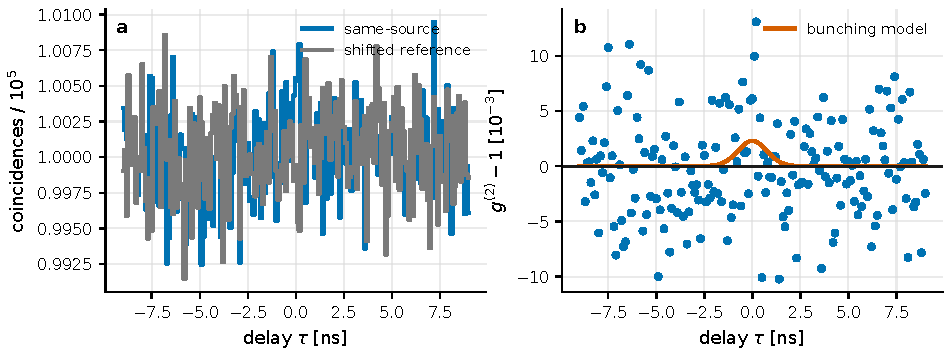
\includegraphics[width=0.95\linewidth]{figures/generated/chapter_04/ch04_delay_histogram_estimator.pdf}
\caption{The structure of the delay-histogram estimator. Left: the histogram of same-source event pairs has, near zero delay, a very small excess of coincidences over the shifted reference histogram; right: normalizing the difference by the number of accidental coincidences gives \(g^{(2)}-1\), with a peak of only the \(10^{-3}\) order. Real observations must further add corrections for dead time, background, and the response function.}
\label{fig:e08-delay-hist}
\end{figure}

\paragraph{Statistical Error: Everything Rests on Counting Enough Event Pairs}
\label{sec:e08-shotnoise}

Where does the precision of the estimator come from? Mainly from the shot noise of the accidental-coincidence pair count. If a given delay bin contains \(N_{\rm pair}\) accidental coincidences, it is Poisson-fluctuating (Chapter \ref{chap:e03}), with standard deviation \(\sqrt{N_{\rm pair}}\), so the relative error is

\begin{equation}
  \sigma\!\left[\widehat g^{(2)}(\tau)\right]\sim\frac{1}{\sqrt{N_{\rm pair}}}.
  \label{eq:e08-shotnoise}
\end{equation}
\begin{formulaexplain}
\(\sigma[\widehat g^{(2)}]\) is the statistical error of the correlation estimator; \(N_{\rm pair}=r_Ar_B\,\delta\tau\,T\) is the number of accidental coincidences in that bin. To push the error below a signal of \(10^{-3}\), one must accumulate an enormous number of event pairs.
\end{formulaexplain}

Let us plug in a set of numbers to feel the difficulty. Take two channels with \(r=10^{6}\,{\rm s^{-1}}\), \(\delta\tau=100\,{\rm ps}=10^{-10}\,{\rm s}\), and \(T=1\,{\rm hr}=3600\,{\rm s}\):
\[
  N_{\rm pair}=r_Ar_B\,\delta\tau\,T
  =(10^6)(10^6)(10^{-10})(3600)
  =3.6\times10^{5},
\]
so the single-bin statistical error is \(\sigma\sim1/\sqrt{3.6\times10^5}\approx1.7\times10^{-3}\). This is almost the same order as Guerin's signal of \(2\times10^{-3}\); that is, one hour and a single delay bin are still far from enough, barely \(1\sigma\). To push the error down to \(10^{-4}\) requires \(N_{\rm pair}\sim10^{8}\), i.e.\ accumulating the pair count from \(3.6\times10^5\) by about \(300\) times more (\(10^8/3.6\times10^5\approx278\)). Note that this factor of 300 scales differently along the two routes: \(N_{\rm pair}\propto T\) is linear in exposure, so the exposure time must be lengthened by about \(300\) times; whereas \(N_{\rm pair}\propto r_Ar_B\) is quadratic in count rate, so raising each channel's count rate by about \(\sqrt{300}\approx17\) times suffices (the third "Questions to Ponder" of this chapter tests exactly this \(r^2\) scaling). Of course one may combine the two, or jointly fit the several bins spanned by the bunching peak (the peak is more than one bin wide, and can be used jointly). This also reminds us of a ceiling: when the systematic correlation (TDC crosstalk, residual background normalization) sits at the \(10^{-3}\) level, adding more exposure cannot substitute for correcting these systematic terms. Modern VERITAS and MAGIC intensity interferometry extends exactly this idea to spatial scales, using offline correlation, GPU/FPGA correlators, and multi-baseline averaging \citep{2020NatAs...4.1164A,2024MNRAS.529.4387A}.

\section{Looking Ahead: Third-Order Correlation and Closure Phase}
\label{sec:e08-g3}

Second-order correlation invokes only photon \emph{pairs}. If we keep three telescopes (or three channels) at once, we can define the third-order intensity correlation:

\begin{equation}
  g^{(3)}_{123}=\frac{\big\langle I_1 I_2 I_3\big\rangle}
  {\big\langle I_1\big\rangle\big\langle I_2\big\rangle\big\langle I_3\big\rangle}.
  \label{eq:e08-g3}
\end{equation}
\begin{formulaexplain}
\(g^{(3)}_{123}\) is the three-channel normalized intensity correlation; \(I_1,I_2,I_3\) are the intensities of the three telescopes; the denominator is the random triple-coincidence baseline. It generalizes the statistical object from "photon pairs" to "photon triplets."
\end{formulaexplain}

For Gaussian chaotic light, one again uses the Gaussian moment theorem to split the sixth-order moment (this time three unstarred and three starred fields paired two by two, with a total of \(3!=6\) legal "starred-with-unstarred" pairings: three of them pair \(I_i\) in place into modulus-squared terms of the \(|\gamma|^2\) type, while a conjugate pair of cyclic pairings combines into the closure term). The result, beyond the modulus-squared terms of the three baselines, contains one extra \emph{triangle closure} term:

\begin{equation}
  g^{(3)}_{123}=1+|\gamma_{12}|^2+|\gamma_{23}|^2+|\gamma_{31}|^2
  +2\,{\rm Re}\!\big(\gamma_{12}\,\gamma_{23}\,\gamma_{31}\big),
  \label{eq:e08-g3-closure}
\end{equation}
\begin{formulaexplain}
\(\gamma_{ij}\) is the first-order degree of coherence (a complex number) between channels \(i,j\); the three modulus-squared terms come from the three baselines; the final term \({\rm Re}(\gamma_{12}\gamma_{23}\gamma_{31})\) is the \textbf{closure phase} term, obtained by adding the phases of the three baselines. It is the entry point by which third-order intensity interferometry reaches phase combinations.
\end{formulaexplain}

The key lies in the final term: in \(\gamma_{12}\gamma_{23}\gamma_{31}\) the phases of the three complex degrees of coherence add up, forming exactly a \emph{closed triangle}. Second-order intensity interferometry gives only \(|\gamma|^2\), throwing the phase away entirely; but this closure phase in the third-order term is measurable. This points directly to the imaging phase problem of Chapter \ref{chap:e11}: intensity interferometry innately loses phase, and the closure phase (along with higher-order correlations) is one route to recovering phase combinations. The price is much greater noise: photon triplets are far rarer than photon pairs, and more sensitive to systematic errors. Gamo's early theory and the imaging simulations of Nuñez et al.\ both treat higher-order correlation as an important extension of intensity-interferometric imaging \citep{1966JOSA...56..441G,2012MNRAS.419..172N}.

\begin{figure}[tbp]
\centering
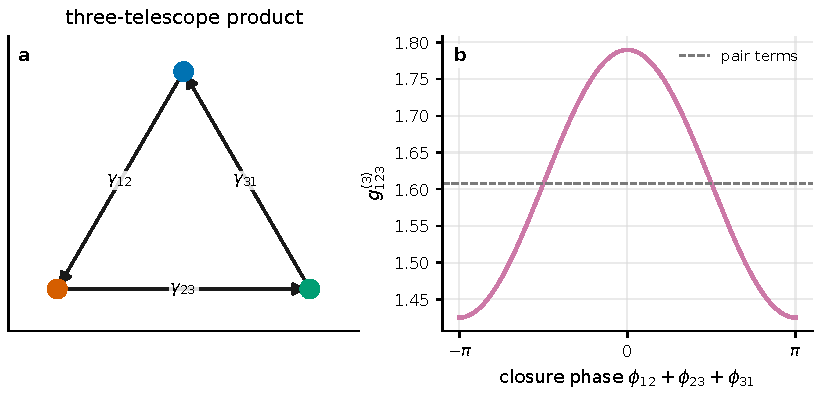
\includegraphics[width=0.92\linewidth]{figures/generated/chapter_04/ch04_g3_closure_phase.pdf}
\caption{The origin of the closure-phase term in the third-order intensity correlation. Left: three telescopes form the closed product \(\gamma_{12}\gamma_{23}\gamma_{31}\); right: at fixed \(|\gamma_{ij}|\), \(g^{(3)}\) varies as the cosine of the closure phase. Second-order intensity interferometry gives only \(|\gamma|^2\); only the third-order term begins to be sensitive to phase combinations.}
\label{fig:e08-g3}
\end{figure}

\section{A Door: Trading the Time Delay for a Spatial Baseline}
\label{sec:e08-gateway}

From start to finish this chapter has spoken of the "time delay \(\tau\)," the echo of the same beam of light across a delay \(\tau\). The final step is to replace the \(\tau\) of this language with a \emph{spatial baseline} \(\bm B\), and a door opens onto Chapter \ref{chap:e10}.

Imagine two telescopes separated by \(\bm B\) staring at the same star at once, each recording intensity fluctuations. Replace the two "instants" of \(g^{(1)}\) with two "positions," and it no longer measures "how much phase the field remembers across \(\tau\)," but "how coherent the field is at two points separated by \(\bm B\)." And the van Cittert--Zernike theorem (to be proved in Chapter \ref{chap:e10}) will tell us: this spatial version of \(g^{(1)}(\bm B)\) is exactly the \textbf{complex visibility} of the sky brightness distribution: it is a Fourier component of the source's angular structure. So the Siegert relation carries over unchanged:

\[
  g^{(2)}(\bm B)-1=\zeta\,\big|g^{(1)}(\bm B)\big|^2
  =\zeta\,\big|V(\bm B)\big|^2 ,
\]

and the \emph{degree of synchrony} of the intensity fluctuations of the two telescopes directly yields the squared modulus of the complex visibility, \(|V(\bm B)|^2\). This is the whole magic of HBT intensity interferometry: without combining the electric fields of the two telescopes through a vacuum pipe as amplitude interferometry does (an almost punishing demand on optical-path stability), one measures the squared visibility simply by comparing, after the fact, the intensity fluctuations recorded separately at the two sites, and thereby infers the star's angular diameter. The prerequisite for validity remains the two conditions this chapter has stressed repeatedly: the source light is approximately Gaussian chaotic light, and the instrument normalization has not mixed the background, mode number, and time response into \(\zeta\).

Carrying this door with us, we can step into Chapter \ref{chap:e10}: upgrading "temporal correlation" into "spatial correlation," upgrading "coherence time" into "visibility curve," and finally, in Chapter \ref{chap:e11}, inferring the image of a celestial object from the visibility.

\section{Chapter Summary}
\label{sec:e08-summary}

\begin{itemize}
  \item \textbf{Two orders of coherence, two plain questions.} First order \(g^{(1)}(\tau)\) (Eq.~\eqref{eq:e08-g1}) measures the phase memory of the field: \(|g^{(1)}|\to1\) coherent, \(\to0\) amnesic, and its decay width is the coherence time \(\tau_c\simeq1/\Delta\nu\) (780\,nm/1\,nm gives \(\tau_c\approx2\,{\rm ps}\)). Second order \(g^{(2)}(\tau)\) (Eq.~\eqref{eq:e08-g2-field}) measures the tendency of photons to arrive in pairs.
  \item \textbf{Three statistics, three peaks.} Poisson (coherent state) \(g^{(2)}=1\); thermal-light bunching \(g^{(2)}(0)=2\); \(g^{(2)}(0)<1\) antibunching, a nonclassical signature. The classical form \(g^{(2)}=\langle II\rangle/\langle I\rangle^2\) is handy, but beware whether \(I\) has already been convolved by the response.
  \item \textbf{The Siegert relation is the bridge of this chapter.} \(g^{(2)}(\tau)=1+\zeta|g^{(1)}(\tau)|^2\) (Eq.~\eqref{eq:e08-siegert}), coming from the fourth-order-moment split of Gaussian chaotic light (the Gaussian-moment/Wick theorem): \(\langle II\rangle=\langle I\rangle^2+|G^{(1)}|^2\). It lets the intensity correlation directly read off the squared field coherence. The spectral shape sets the peak shape: rectangular sinc\(^2\), Lorentzian exponential, Gaussian Gaussian. \(\zeta\) collects only mode number, polarization, and background (the finite time response is handled separately by convolution and is not included in \(\zeta\)). \emph{It does not hold for coherent states.}
  \item \textbf{Dilution in the telescope.} The finite-response convolution preserves area but not peak height, \(C_{\rm obs}\simeq C_{\rm true}(\tau_c/\Delta t_{\rm eff})(1/M)f_Af_B\) (Eq.~\eqref{eq:e08-contrast}). Guerin's experiment: \(7800\,\text{\AA}\), \(10\,\text{\AA}\), \(\tau_c\approx2\,{\rm ps}\), response \(\approx700\,{\rm ps}\), observed peak only \(C_{\rm obs}\approx2\times10^{-3}\).
  \item \textbf{Estimator and noise.} The delay histogram \(\widehat g^{(2)}=H_{AB}/(r_Ar_B\,\delta\tau\,T)\) (Eq.~\eqref{eq:e08-estimator}), with error \(\sigma\sim N_{\rm pair}^{-1/2}\) (Eq.~\eqref{eq:e08-shotnoise}): everything rests on counting enough event pairs.
  \item \textbf{Two doors.} The closure-phase term of the third-order \(g^{(3)}\) leads to the imaging phase problem of Chapter \ref{chap:e11}; replacing \(\tau\) with the baseline \(\bm B\) turns \(g^{(1)}\) into the complex visibility \(V(\bm B)\), leading to the spatial intensity interferometry of Chapter \ref{chap:e10}.
\end{itemize}

\medskip
\noindent\textbf{Questions to Ponder.}
\begin{enumerate}
  \item If the filter bandwidth is broadened from \(10\,\text{\AA}\) to \(100\,\text{\AA}\), how does the coherence time \(\tau_c\) change? With the response \(\Delta t_{\rm eff}\approx700\,{\rm ps}\) unchanged, will the observed peak height \(C_{\rm obs}\) rise or fall, and by roughly what factor?
  \item Someone measures a source whose \(g^{(1)}\) remains close to 1 over very long delays, yet finds \(g^{(2)}\equiv1\). Is this more likely thermal light or a laser? Why does it not violate the Siegert relation?
  \item If the count rates of the two channels are each raised by 10 times and the exposure time lengthened by 4 times, by what factor does the single-bin accidental-coincidence number \(N_{\rm pair}\) change? And by what factor does the corresponding statistical error \(\sigma[\widehat g^{(2)}]\) change?
\end{enumerate}


% ============================================================
\part{Coherence, Interference, and Imaging}
\chapter{Temporal Coherence and First-Order (Amplitude) Interferometry}
\label{chap:e09}

\begin{chapteropening}
By now we know that light is the excitation of a set of modes, whose positive-frequency field operator \(\hat E^{(+)}\) was introduced in Chapter \ref{chap:e05}; and that a detector counts only intensity and cannot see the phase of the field is exactly what the photodetection of Chapter \ref{chap:e07} taught us (one optical cycle is only a few femtoseconds, so any detector is far too "slow," and can only average away the oscillation and leave the energy). We also know that a beam of light "remembers its own phase" only for a coherence time \(\tau_c\simeq1/\Delta\nu\) (Chapter \ref{chap:e02}). But if the phase cannot be seen, on what grounds do we speak of "coherence"? The answer is interference: split a beam into two paths, send them along different optical paths, and recombine them, and the phase difference will show itself in the \emph{intensity}: bright fringes, dark fringes, one after another. What this chapter does is bring the abstract first-order degree of coherence \(g^{(1)}(\tau)\) down to a tangible interferometer you can see and touch: we derive the fringe-intensity formula, define the fringe visibility, and prove that "the visibility is the direct reading of how much phase the field still remembers"; then, following the Wiener--Khinchin theorem, we build a bridge explaining why "how fast the fringes fade with optical-path difference" can, remarkably, tell us in reverse the shape of the spectral line; this is precisely the principle of Fourier-transform spectroscopy. Finally we generalize this "time-delay version" of coherence into a "two-point spatial version," and hand it over to the next chapter's van Cittert--Zernike theorem and intensity interferometry.
\end{chapteropening}

\section{From One Optical Path to Two}
\label{sec:e09-two-beams}

Let us first draw the interferometer. The cleanest example is the Michelson interferometer: a beam of light strikes a beam splitter, half heading toward a fixed mirror and half toward a movable mirror; each returns along its own path and recombines behind the beam splitter, and both fall onto the same detector. The two optical paths are generally unequal in length, differing by an optical-path difference \(\Delta\) (in cm). Young's double slit is its geometric sibling: the same beam passes through two slits, and in reaching a point on the screen it too has traversed two unequal segments, except that there the path difference comes from two sampling points in \emph{space}, a point we will return to at the end of this chapter. For now, let us fix our gaze on the temporal version of Michelson's "same beam, two optical paths."

The field on the detector surface is the superposition of the two path fields:
\[
  \hat E_{\rm det}(t)=\hat E_1(t)+\hat E_2(t),
\]
where \(\hat E_1\), \(\hat E_2\) are the positive-frequency field operators reaching the detector from the two paths (Chapter \ref{chap:e05}). The detector is "too slow," it averages away the cycle-by-cycle oscillation, and what remains is the intensity averaged over the response time, proportional to the squared modulus of the field. So the mean intensity at this point is
\[
  I=\big\langle \hat E_{\rm det}^{(-)}(t)\,\hat E_{\rm det}^{(+)}(t)\big\rangle
   =\big\langle |\hat E_1+\hat E_2|^2\big\rangle .
\]
Expand the squared modulus. This is the most ordinary algebra, \(|a+b|^2=|a|^2+|b|^2+a^\ast b+ab^\ast\), and taking the average term by term:
\[
  I=\underbrace{\big\langle|\hat E_1|^2\big\rangle}_{I_1}
   +\underbrace{\big\langle|\hat E_2|^2\big\rangle}_{I_2}
   +\big\langle \hat E_1^\ast \hat E_2\big\rangle
   +\big\langle \hat E_1 \hat E_2^\ast\big\rangle .
\]
The first two terms \(I_1,I_2\) are the intensities of each path alone (block the other and only it remains). The last two are complex conjugates of one another, and two complex conjugates added equal twice the real part, so
\begin{equation}
  I=I_1+I_2+2\,\mathrm{Re}\big\langle \hat E_1^\ast(t)\,\hat E_2(t)\big\rangle .
  \label{eq:e09-interference-raw}
\end{equation}
\begin{formulaexplain}
\(I_1,I_2\) are the intensities of the two paths; the final cross term \(\langle\hat E_1^\ast\hat E_2\rangle\) is the correlation of "how much the two path fields still remember of each other." Everything about interference is hidden in this one term.
\end{formulaexplain}

Let us account for each term. \(I_1,I_2\) carry the dimensions of intensity (in CGS, on the order of \({\rm erg\,s^{-1}\,cm^{-2}}\); here we use only their relative magnitude). What truly carries information is the cross term \(\langle\hat E_1^\ast(t)\hat E_2(t)\rangle\): if the two path fields are unrelated, this average is zero, and the detector shows only the flat \(I_1+I_2\), no fringes; if the two path fields are highly correlated, the cross term is large, and sweeping the optical-path difference brings out fringes of strong bright-dark contrast. So \textbf{the depth of the fringes is a direct measure of this cross correlation}.

Now we must work out the cross term precisely. The key physical fact is: path 2 is merely path 1's beam delayed and shifted by an optical path \(\Delta\): they come from the same source field, just taken at different instants. Writing the normalized complex field as \(\varepsilon(t)\) (satisfying \(\langle|\varepsilon|^2\rangle=1\)), the two paths can be written
\[
  \hat E_1(t)=\sqrt{I_1}\,\varepsilon(t),\qquad
  \hat E_2(t)=\sqrt{I_2}\,\varepsilon(t-\tau),\qquad
  \tau=\frac{\Delta}{c}.
\]
Here \(\tau=\Delta/c\) is the optical-path difference converted into a \emph{time delay} (in s), and \(c\) is the speed of light. The field of path 2 is just the field of path 1 taken \(\tau\) earlier. So the cross term becomes the correlation of the same field at two instants separated by \(\tau\):
\[
  \big\langle \hat E_1^\ast(t)\,\hat E_2(t)\big\rangle
  =\sqrt{I_1 I_2}\,\big\langle \varepsilon^\ast(t)\,\varepsilon(t-\tau)\big\rangle .
\]
What appears here is \(\varepsilon(t-\tau)\) (path 2 delayed by \(\tau\)), whereas the standard definition of \(g^{(1)}\) below is written with \(\varepsilon(t+\tau)\): the two differ by a complex conjugate, so do not rush to equate them. Using stationarity (the correlation depends only on the delay, not on the absolute instant), shift the time origin \(t\to t+\tau\):
\[
  \big\langle \varepsilon^\ast(t)\,\varepsilon(t-\tau)\big\rangle
  =\big\langle \varepsilon^\ast(t+\tau)\,\varepsilon(t)\big\rangle
  =\big[g^{(1)}(\tau)\big]^\ast=g^{(1)}(-\tau) .
\]
Fortunately, what finally enters Eq.~\eqref{eq:e09-interference-raw} is only the \emph{real part} of this term, and its \emph{modulus} will be used; and \(|g^{(1)}|\) is an even function, while the real part is unchanged under complex conjugation, so rewriting it directly as \(g^{(1)}(\tau)\) has \emph{no effect whatsoever} on the modulus and real part of the fringes. Accordingly, it is precisely the first-order degree of coherence (first-order/amplitude coherence) defined in Chapter \ref{chap:e08}. Write the normalized first-order temporal degree of coherence as
\begin{equation}
  g^{(1)}(\tau)=
  \frac{\big\langle \varepsilon^\ast(t)\,\varepsilon(t+\tau)\big\rangle}
       {\big\langle |\varepsilon(t)|^2\big\rangle},
  \qquad g^{(1)}(0)=1 ,
  \label{eq:e09-g1-def}
\end{equation}
\begin{formulaexplain}
\(g^{(1)}(\tau)\) is the correlation of the same beam's field separated by \(\tau\), normalized by dividing by its own intensity. It is complex: the modulus \(|g^{(1)}|\) says "how much is remembered," and the argument says "how much the phase has shifted." At \(\tau=0\) the field is fully correlated with itself, \(g^{(1)}(0)=1\).
\end{formulaexplain}
where \(\tau\) is the time delay (in s) and \(g^{(1)}\) is dimensionless. It is complex: \(|g^{(1)}(\tau)|\) decays from 1 (\(\tau=0\), fully coherent) to 0 (phase memory entirely lost) as the delay increases; its argument records the phase difference. For a stationary light field, this correlation depends only on the delay \(\tau\), not on the absolute instant \(t\), a point we will use again and again.

Now substitute the cross term back into Eq.~\eqref{eq:e09-interference-raw}. Here we must make a split that is physically crucial. The phase of the degree of coherence \(g^{(1)}(\tau)\) in fact mixes two things of completely different speeds: one is the carrier phase, from the oscillation accumulated by the optical-path difference at the central frequency \(\bar\nu\); the other is a slowly varying residual phase. Because every time the optical-path difference changes by one wavelength \(\lambda\) the carrier phase turns through a full \(2\pi\) while \(|g^{(1)}|\) barely stirs, it is most natural to factor the carrier out. First define the carrier phase
\[
  \delta=\frac{2\pi\Delta}{\lambda}=2\pi\bar\nu\,\tau ,
\]
then \emph{divide} this carrier out of \(g^{(1)}\), obtaining a complex quantity that varies only slowly, written \(\tilde g(\tau)\) (note it is a \emph{new symbol}, not \(\arg g^{(1)}\) itself):
\[
  \tilde g(\tau)\equiv e^{+i2\pi\bar\nu\tau}\,g^{(1)}(\tau)
  =\big|g^{(1)}(\tau)\big|\,e^{\,i\varphi(\tau)} .
\]
Multiplying by a phase factor of unit modulus does not change the modulus, so \(|\tilde g|=|g^{(1)}|\); here \(\varphi(\tau)\) is the \emph{slowly varying residual phase left after removing the carrier} (dimensionless, in rad), and it is \(\varphi\equiv0\) when the spectral line is symmetric. Solving this definition back for \(g^{(1)}\):
\[
  g^{(1)}(\tau)=e^{-i2\pi\bar\nu\tau}\,\tilde g(\tau)
  =\big|g^{(1)}(\tau)\big|\,e^{\,i[\varphi(\tau)-\delta]} .
\]
So taking the real part (\(\cos\) is even, \(\cos(\varphi-\delta)=\cos(\delta-\varphi)\)) gives \(\mathrm{Re}\,g^{(1)}=|g^{(1)}|\cos\!\big(\delta-\varphi(\tau)\big)\), and substituting back into Eq.~\eqref{eq:e09-interference-raw} gives the central result of this section: the fringe formula for two-beam interference:
\begin{equation}
  I(\delta)=I_1+I_2+2\sqrt{I_1 I_2}\;\big|g^{(1)}(\tau)\big|\,
  \cos\!\big(\delta-\varphi(\tau)\big),
  \qquad \delta=\frac{2\pi\Delta}{\lambda},\ \ \tau=\frac{\Delta}{c}.
  \label{eq:e09-fringe}
\end{equation}
\begin{formulaexplain}
Fringe intensity = the two-path floor \(I_1+I_2\) + a cosine term that ripples with the optical-path difference. The cosine makes bright and dark alternate, and its \emph{amplitude} is proportional to \(|g^{(1)}(\tau)|\): the more the field remembers, the deeper the fringes ripple. The carrier phase \(\delta=2\pi\Delta/\lambda\) is the knob we turn by moving the mirror; \(\varphi(\tau)\) is the slow residual phase after removing the carrier, zero when the spectral line is symmetric.
\end{formulaexplain}

Let us read this formula thoroughly. \(\delta=2\pi\Delta/\lambda\) is the phase directly controlled by moving the mirror: translate the mirror by half a wavelength (the optical-path difference changes by one wavelength) and \(\delta\) turns through \(2\pi\), the fringes running through one bright-and-dark cycle. So as we scan \(\Delta\), the detector reading swings back and forth between \(I_{\max}\) and \(I_{\min}\); these are the fringes. The amplitude of the swing is \(2\sqrt{I_1 I_2}\,|g^{(1)}(\tau)|\): it has two factors, \(2\sqrt{I_1I_2}\) being how well the two path intensities are matched (maximal at equal intensity), and \(|g^{(1)}(\tau)|\) being how much phase the field still remembers after the delay \(\tau\). If \(|g^{(1)}|=1\), the fringes swing at full amplitude about \(I_1+I_2\); if \(|g^{(1)}|=0\), the cosine term vanishes and the detector shows a uniform field, no fringes. In other words: \textbf{the presence and depth of the fringes is the direct development of the first-order coherence}. In the next section we quantify "depth" into a standard number.

\section{The Fringe Visibility Is the Reading of the Degree of Coherence}
\label{sec:e09-visibility}

Look at fringes with the naked eye, and the first impression is "how clear they are": strong contrast between bright and dark is clear, weak contrast is blurry. To turn this impression into a measurable number is the fringe visibility, first introduced by Michelson:
\begin{equation}
  \mathcal V=\frac{I_{\max}-I_{\min}}{I_{\max}+I_{\min}} .
  \label{eq:e09-visibility-def}
\end{equation}
\begin{formulaexplain}
\(\mathcal V\) divides the contrast of the brightest fringe \(I_{\max}\) and the darkest fringe \(I_{\min}\) by their sum. From all-dark to all-bright \(\mathcal V=1\); a uniform gray with no fringes gives \(\mathcal V=0\). It is the standard scale of "how clear the fringes are."
\end{formulaexplain}
\(I_{\max}\), \(I_{\min}\) are, respectively, the maximum and minimum intensities the detector reads while scanning \(\delta\); \(\mathcal V\) is dimensionless, between 0 and 1. Why use this combination rather than another? Because it \emph{automatically cancels the total brightness}: double the source brightness, and \(I_{\max},I_{\min}\) double together, leaving the ratio unchanged. Visibility cares only about "contrast," not about "how bright," which is exactly what we want to ask about "coherence."

Now substitute Eq.~\eqref{eq:e09-fringe}. As \(\delta\) is scanned, the cosine takes values between \(+1\) and \(-1\) (the residual phase \(\varphi(\tau)\) varies very slowly, and on the scale of a single fringe can be treated as constant, merely shifting the fringes as a whole a little and not changing the peak and trough heights):
\[
  I_{\max}=I_1+I_2+2\sqrt{I_1 I_2}\,|g^{(1)}(\tau)|
  \quad(\cos=+1),
\]
\[
  I_{\min}=I_1+I_2-2\sqrt{I_1 I_2}\,|g^{(1)}(\tau)|
  \quad(\cos=-1).
\]
Subtracting the two, the floor \(I_1+I_2\) cancels, leaving twice the cosine amplitude:
\[
  I_{\max}-I_{\min}=4\sqrt{I_1 I_2}\,|g^{(1)}(\tau)| .
\]
Adding the two, the cosine amplitude cancels, leaving twice the floor:
\[
  I_{\max}+I_{\min}=2\,(I_1+I_2).
\]
Dividing, the common 2 cancels, giving the bridge between visibility and the degree of coherence:
\begin{equation}
  \mathcal V(\tau)=\frac{2\sqrt{I_1 I_2}}{I_1+I_2}\,\big|g^{(1)}(\tau)\big| .
  \label{eq:e09-visibility-g1}
\end{equation}
\begin{formulaexplain}
Visibility = the intensity-matching factor \(2\sqrt{I_1I_2}/(I_1+I_2)\) times the coherence modulus \(|g^{(1)}(\tau)|\). The former depends only on the ratio of the two path brightnesses; the latter is the coherence of the light itself. At equal intensity the former is 1, and the visibility \emph{is} \(|g^{(1)}|\).
\end{formulaexplain}

This formula cleanly separates two things. The first factor \(2\sqrt{I_1 I_2}/(I_1+I_2)\) is purely a geometric match: it is the geometric mean of the two path intensities over their arithmetic mean, always \(\le 1\), equal to 1 only when \(I_1=I_2\) (this is the mean inequality, geometric mean equals arithmetic mean if and only if the two numbers are equal). It measures whether "the instrument has adjusted the two paths to equal brightness," and has nothing to do with the coherence of the light. The second factor \(|g^{(1)}(\tau)|\) is the physical protagonist. So in experiments one always deliberately tunes the two paths to equal intensity \(I_1=I_2\), whereupon the matching factor is 1 and visibility equals the degree of coherence directly:
\begin{equation}
  \boxed{\;\mathcal V(\tau)=\big|g^{(1)}(\tau)\big|\quad(I_1=I_2)\;}
  \label{eq:e09-visibility-equals-g1}
\end{equation}
\begin{formulaexplain}
At equal intensity, the fringe clarity \(\mathcal V\) you measure on the interferogram \emph{is} the modulus \(|g^{(1)}(\tau)|\) of that abstract first-order degree of coherence. The abstract "how much phase the field still remembers" becomes visible fringe contrast.
\end{formulaexplain}

This is the first sentence this chapter wants you to remember: \textbf{the fringe visibility is the direct reading of "how much phase the field still remembers."} In Chapter \ref{chap:e08}, \(g^{(1)}\) was an abstract object written inside an operator average, which you could not directly "see"; now it has an avatar readable by eye: set the interferometer's delay to \(\tau\), count the contrast between bright and dark fringes, and what you get is \(|g^{(1)}(\tau)|\). The phase, that thing the detector "cannot see," leaves its shadow on the intensity through interference, and the visibility is the depth of that shadow.

Incidentally, the two extremes of the equal-intensity double slit are easy to remember: \(\mathcal V=1\) means fully coherent, the fringes running from all-dark to all-bright, corresponding in astronomy to "this baseline has not yet resolved the source at all"; \(\mathcal V=0\) means fully incoherent, the screen showing only the flat superposition of each slit's illumination, no fringes, corresponding to "the source is completely resolved at this scale and the coherence has been washed out." Real observations almost always fall between the two, and the visibility is a decimal between 0 and 1, whose specific value carries the information we want.

\section{Coherence Length and Coherence Time}
\label{sec:e09-coherence-length}

Equation~\eqref{eq:e09-visibility-equals-g1} says the visibility varies with the delay \(\tau\). But how does it vary? The physical intuition is clear: the larger the delay, the older the field path 2 takes, and light "remembers its own phase" only for a coherence time \(\tau_c\simeq1/\Delta\nu\) (Chapter \ref{chap:e02}); once the delay exceeds \(\tau_c\), the phases of the two paths have long gone their separate ways and lost their correlation, \(|g^{(1)}|\to0\), and the fringes vanish with it. So:

\begin{quote}
\textbf{The fringes fade as the optical-path difference grows, and the characteristic scale of this decay is the coherence length.}
\end{quote}

Convert the coherence time into the distance light travels, and it is the coherence length:
\begin{equation}
  \ell_c=c\,\tau_c\simeq\frac{c}{\Delta\nu}\simeq\frac{\lambda^2}{\Delta\lambda},
  \qquad
  \Delta\nu\simeq\frac{c\,\Delta\lambda}{\lambda^2}.
  \label{eq:e09-coherence-length}
\end{equation}
\begin{formulaexplain}
\(\ell_c\) is the largest scale (in cm) of optical-path difference over which fringes can still be seen. It equals the coherence time \(\tau_c\) times the speed of light. The wider the bandwidth \(\Delta\nu\) (or the larger \(\Delta\lambda\)), the shorter the coherence length and the sooner the fringes vanish.
\end{formulaexplain}
Let us account for each term. \(\ell_c\) is in cm (or m); \(\tau_c\) is the coherence time (s); \(\Delta\nu\) is the frequency bandwidth (Hz); \(\lambda\) is the central wavelength, \(\Delta\lambda\) the wavelength bandwidth. The last-step bandwidth conversion \(\Delta\nu\simeq c\,\Delta\lambda/\lambda^2\) comes from differentiating \(\nu=c/\lambda\) (\(|{\rm d}\nu|=(c/\lambda^2)|{\rm d}\lambda|\)), consistent with Chapter \ref{chap:e02}. The physical meaning in one sentence: \emph{once the two-path optical-path difference exceeds \(\ell_c\), the fringes are essentially invisible}. It is the hard specification for "how much optical-path mismatch the interferometer can tolerate."

Substitute real numbers to feel how many orders of magnitude this scale spans.

\paragraph{White light.} The white light seen by the naked eye has an extremely broad bandwidth; take \(\lambda\simeq550\,{\rm nm}\), \(\Delta\lambda\simeq300\,{\rm nm}\) (the whole visible):
\[
  \Delta\nu\simeq\frac{(3\times10^{10}\,{\rm cm\,s^{-1}})(3\times10^{-5}\,{\rm cm})}
  {(5.5\times10^{-5}\,{\rm cm})^2}\simeq3\times10^{14}\,{\rm Hz},
  \quad
  \tau_c\simeq3.4\times10^{-15}\,{\rm s},
  \quad
  \ell_c\simeq1\,\mu{\rm m}.
\]
The coherence length of white light is only about a micron, two or three wavelengths! This is exactly why, viewing Michelson interference with white light, colored fringes appear only in a small range where the two arms are almost exactly equal, blurring away at the slightest shift. It also explains why the colored interference on soap films and oil films appears only when the film is very thin.

\paragraph{Narrowband filter.} Add a \(\Delta\lambda=1\,{\rm nm}\) filter, central \(\lambda=550\,{\rm nm}\): \(\Delta\nu\simeq1\times10^{12}\,{\rm Hz}\), \(\tau_c\simeq1\,{\rm ps}\), \(\ell_c\simeq0.3\,{\rm mm}\). The coherence length jumps at once to submillimeter: now the two arms may differ by a few tenths of a millimeter and fringes are still seen. Guerin et al.'s stellar bunching experiment used exactly this order: \(\lambda\simeq780\,{\rm nm}\), \(\Delta\lambda=1\,{\rm nm}\) gives \(\tau_c\simeq2\,{\rm ps}\), \(\ell_c\simeq0.6\,{\rm mm}\) \citep{2017MNRAS.472.4126G}.

\paragraph{Laser.} A single-frequency laser can have a bandwidth as narrow as \(\Delta\nu=1\,{\rm MHz}\): \(\tau_c=1\,\mu{\rm s}\), \(\ell_c=c\tau_c=300\,{\rm m}\). A coherence length of hundreds of meters: this is why lasers can do long-arm interferometry (even kilometer-scale arm lengths, as in gravitational-wave detectors) while white light never could. Compress the bandwidth further to kHz, and the coherence length enters hundreds of kilometers.

A single table brings this picture, spanning more than a dozen orders of magnitude, into one view: from the micron of white light, to the submillimeter of narrowband, to the hundred meters of the laser, the coherence length is set entirely by bandwidth. Remember this chain; it returns every time we later ask "how much delay/optical-path difference can be tolerated."

\section{The Wiener--Khinchin Bridge: Fringe Decay Infers the Spectral Line}
\label{sec:e09-wiener-khinchin}

The previous section said \(|g^{(1)}(\tau)|\) decays with \(\tau\) on the coherence-time scale, but did not say \emph{by what shape} it decays: slow then fast, exponential decline, or oscillating downward? This shape is not arbitrary; it is uniquely determined by the \textbf{spectral line shape} of the light. What makes this relationship clear is the Wiener--Khinchin theorem: \(g^{(1)}(\tau)\) and the normalized power spectrum are Fourier transforms of each other. This bridge has a striking corollary: \emph{measure how the fringes decay with delay and you can infer what the spectral line looks like}, which is precisely the principle of Fourier-transform spectroscopy. Chapter \ref{chap:e02} previewed it; here we establish it self-containedly.

The derivation needs only one physical input: the different frequency components of a stationary light field are mutually uncorrelated. First expand the complex field by frequency (this is the Fourier analysis of Chapter \ref{chap:e02}, keeping only the positive-frequency part, corresponding to \(\hat E^{(+)}\) of Chapter \ref{chap:e05}):
\[
  \varepsilon(t)=\int_0^\infty \tilde\varepsilon(\nu)\,e^{-i2\pi\nu t}\,{\rm d}\nu,
  \qquad
  \varepsilon^\ast(t)=\int_0^\infty \tilde\varepsilon^\ast(\nu')\,e^{+i2\pi\nu' t}\,{\rm d}\nu' .
\]
where \(\tilde\varepsilon(\nu)\) is the complex amplitude at frequency \(\nu\). Multiply the two and write the first-order correlation over the delay \(\tau\), \(G^{(1)}(\tau)=\langle\varepsilon^\ast(t)\varepsilon(t+\tau)\rangle\):
\[
  G^{(1)}(\tau)
  =\int_0^\infty\!\!\int_0^\infty
  \big\langle \tilde\varepsilon^\ast(\nu')\,\tilde\varepsilon(\nu)\big\rangle\,
  e^{+i2\pi\nu' t}\,e^{-i2\pi\nu(t+\tau)}\,{\rm d}\nu\,{\rm d}\nu' .
\]
Now use that one physical input. The light field is \emph{stationary} (its statistical properties do not change with the time origin), which mathematically forces the different frequency components to be mutually uncorrelated, with nonzero correlation only at the same frequency. This is a standard result (the spectral representation theorem of stationary processes, which may be taken as known):
\[
  \big\langle \tilde\varepsilon^\ast(\nu')\,\tilde\varepsilon(\nu)\big\rangle
  =S(\nu)\,\delta(\nu-\nu') ,
\]
where \(S(\nu)\ge0\) is the power spectral density (that is, the spectral line shape), and \(\delta\) is the Dirac function. It must be so, because if the correlation for \(\nu\ne\nu'\) were nonzero, the above would retain a factor like \(e^{i2\pi(\nu'-\nu)t}\) containing \(t\), destroying the stationarity that "the result depends only on \(\tau\), not on \(t\)." After substitution, \(\delta(\nu-\nu')\) devours one integral (setting \(\nu'=\nu\)), and the \(t\)-containing exponentials \(e^{+i2\pi\nu t}e^{-i2\pi\nu t}=1\) cancel exactly:
\[
  G^{(1)}(\tau)=\int_0^\infty S(\nu)\,e^{-i2\pi\nu\tau}\,{\rm d}\nu .
\]
Finally divide by the value at \(\tau=0\), \(G^{(1)}(0)=\int S(\nu)\,{\rm d}\nu\) (the total power), to normalize, giving the Wiener--Khinchin theorem:
\begin{equation}
  g^{(1)}(\tau)=
  \frac{\displaystyle\int_0^\infty S(\nu)\,e^{-i2\pi\nu\tau}\,{\rm d}\nu}
       {\displaystyle\int_0^\infty S(\nu)\,{\rm d}\nu} .
  \label{eq:e09-wiener-khinchin}
\end{equation}
\begin{formulaexplain}
The first-order degree of coherence \(g^{(1)}(\tau)\) is the Fourier transform of the normalized power spectrum \(S(\nu)\). The wider the spectral line, the faster \(g^{(1)}\) decays (the shorter the coherence time); the specific shape of the spectral line determines the specific shape of the fringe envelope.
\end{formulaexplain}
\(S(\nu)\) is the power spectral density (spectral line shape), \(\nu\) in Hz; the denominator normalizes the total power, ensuring \(g^{(1)}(0)=1\). This formula locks "coherence in the time domain" and "the spectral line in the frequency domain" into a Fourier-transform pair. It immediately gives the origin of the previous section's coherence time: the wider the spectral line (the larger \(\Delta\nu\)), the narrower its Fourier transform (the smaller \(\tau_c\simeq1/\Delta\nu\)), and the sooner the fringes vanish. The two examples below work out the correspondence "spectral line shape \(\to\) fringe decay shape" concretely, both using standard Fourier-transform pairs.

\paragraph{Example 1: rectangular spectrum \(\to\) sinc decay.} Let the spectral line be a rectangle of width \(\Delta\nu\) centered at \(\bar\nu\) (an ideal flat-topped narrowband filter), normalized to \(S(\nu)=1/\Delta\nu\) (within the band), and substitute into Eq.~\eqref{eq:e09-wiener-khinchin}. Let \(\nu=\bar\nu+f\), \(f\in[-\Delta\nu/2,\,\Delta\nu/2]\):
\[
  g^{(1)}(\tau)=\frac{1}{\Delta\nu}\int_{-\Delta\nu/2}^{\Delta\nu/2}
  e^{-i2\pi(\bar\nu+f)\tau}\,{\rm d}f
  =\frac{e^{-i2\pi\bar\nu\tau}}{\Delta\nu}
  \int_{-\Delta\nu/2}^{\Delta\nu/2}e^{-i2\pi f\tau}\,{\rm d}f .
\]
Inside is the most basic exponential integral \(\int e^{-i2\pi f\tau}{\rm d}f=e^{-i2\pi f\tau}/(-i2\pi\tau)\); substituting the limits and using \(e^{-ix}-e^{+ix}=-2i\sin x\):
\[
  \int_{-\Delta\nu/2}^{\Delta\nu/2}e^{-i2\pi f\tau}\,{\rm d}f
  =\frac{e^{-i\pi\Delta\nu\tau}-e^{+i\pi\Delta\nu\tau}}{-i2\pi\tau}
  =\frac{-2i\sin(\pi\Delta\nu\tau)}{-i2\pi\tau}
  =\frac{\sin(\pi\Delta\nu\tau)}{\pi\tau} .
\]
Dividing by \(\Delta\nu\) and assembling the standard sinc function \({\rm sinc}(x)\equiv\sin(\pi x)/(\pi x)\):
\begin{equation}
  g^{(1)}(\tau)=e^{-i2\pi\bar\nu\tau}\,\frac{\sin(\pi\Delta\nu\tau)}{\pi\Delta\nu\tau}
  =e^{-i2\pi\bar\nu\tau}\,{\rm sinc}(\Delta\nu\,\tau),
  \qquad
  \big|g^{(1)}(\tau)\big|=\big|{\rm sinc}(\Delta\nu\,\tau)\big| .
  \label{eq:e09-rect-sinc}
\end{equation}
\begin{formulaexplain}
A rectangular spectrum gives a sinc-type visibility: the fringes first decay with delay as a sinc, hit zero for the first time at \(\tau=1/\Delta\nu\), and then have a train of ever-shorter sidelobes. The position of the first zero marks the bandwidth.
\end{formulaexplain}
The visibility \(\mathcal V=|g^{(1)}|=|{\rm sinc}(\Delta\nu\tau)|\) first drops to zero at \(\tau=1/\Delta\nu=\tau_c\), and thereafter has a train of ever-shorter sidelobes (the subsidiary peaks of the sinc). The factor \(e^{-i2\pi\bar\nu\tau}\) is that fast carrier: \(2\pi\bar\nu\tau=2\pi\Delta/\lambda=\delta\), exactly the carrier phase we factored out in Eq.~\eqref{eq:e09-fringe} to scan as a knob (i.e.\ \(e^{-i2\pi\bar\nu\tau}=e^{-i\delta}\)). At this point the carrier-removed complex quantity \(\tilde g(\tau)=e^{+i2\pi\bar\nu\tau}g^{(1)}(\tau)={\rm sinc}(\Delta\nu\tau)\) is \emph{real}, so the residual phase \(\varphi(\tau)\equiv0\) (the rectangular spectrum is symmetric), matching exactly the split of Section \ref{sec:e09-two-beams}. Note that \(|g^{(1)}|^2={\rm sinc}^2(\Delta\nu\tau)\) is precisely the second-order bunching-peak shape appearing in the Siegert relation of Chapter \ref{chap:e08}: the two chapters meet here.

\paragraph{Example 2: Lorentzian spectrum \(\to\) exponential decay.} Many spectral lines (collisional broadening, natural linewidth, single-mode cavity leakage) are Lorentzian: \(S(\nu)\propto 1/[(\nu-\bar\nu)^2+(\Delta\nu/2)^2]\), where \(\Delta\nu\) is the full width at half maximum (FWHM). The Fourier transform of a Lorentzian is a two-sided decaying exponential: this is a standard Fourier-transform pair (Lorentzian \(\leftrightarrow\) exponential), cited directly:
\begin{equation}
  g^{(1)}(\tau)=e^{-i2\pi\bar\nu\tau}\,e^{-\pi\Delta\nu\,|\tau|}
  =e^{-i2\pi\bar\nu\tau}\,e^{-|\tau|/\tau_c},
  \qquad
  \tau_c=\frac{1}{\pi\Delta\nu} .
  \label{eq:e09-lorentz-exp}
\end{equation}
\begin{formulaexplain}
A Lorentzian spectrum gives a purely exponentially decaying visibility \(|g^{(1)}|=e^{-|\tau|/\tau_c}\), with no zeros and no sidelobes, sliding down smoothly all the way. The decay constant \(\tau_c=1/(\pi\Delta\nu)\) directly gives the linewidth.
\end{formulaexplain}
Now \(|g^{(1)}(\tau)|=e^{-|\tau|/\tau_c}\) is a smooth exponential decay, with no zeros and no sidelobes, in sharp contrast to the oscillation of the rectangular spectrum. It corresponds to the exponential-type second-order correlation peak given by the Siegert relation in Chapter \ref{chap:e08}. Measuring the fringes decay as a pure exponential with delay is equivalent to measuring that the spectral line is Lorentzian, and the decay constant \(\tau_c\) in turn gives the linewidth \(\Delta\nu=1/(\pi\tau_c)\).

This is the entire logic of Fourier-transform spectroscopy: instead of using a prism or grating to spread the frequencies out one by one, \emph{scan the interferometer's delay}, record the visibility \(\mathcal V(\tau)=|g^{(1)}(\tau)|\) (along with the phase), and then take a Fourier inverse transform of this curve, and the spectral line \(S(\nu)\) is recovered. Its power lies in that the resolution is set by the \emph{maximum delay}: the larger the delay reachable, the finer the frequency resolution. For those extremely narrow spectral lines in astronomy that ordinary spectrographs can hardly reach (such as candidate astrophysical laser lines near \(\eta\) Car, requiring a resolution of \(R\sim10^8\)), using the decay of coherence with delay to infer the linewidth is often the only feasible route. Figure \ref{fig:e09-fourier-visibility} displays this "structure \(\leftrightarrow\) visibility" Fourier correspondence with several source structures; though it draws the spatial version (the subject of the next section), the Fourier skeleton is completely isomorphic to the temporal version here.

\section{Two Routes: Amplitude Interferometry and Intensity Interferometry}
\label{sec:e09-two-routes}

Up to here everything we have discussed is amplitude interferometry: combine the \emph{electric fields} of the two paths physically in optics, let them add and interfere, and read the complex visibility \(\mathcal V\,e^{i\varphi(\tau)}\) from the fringes (\(\varphi\) being the residual phase after subtracting the known carrier \(\delta\)). Its greatest advantage is that \textbf{the phase can also be measured}: the position of the fringe peak relative to the carrier directly gives \(\varphi(\tau)\), which is crucial for imaging. But it has a harsh price: since the interference occurs at the level of the electric field, the two optical paths must be stable to a \emph{fraction of a wavelength}. Visible wavelengths are half a micron, and if the optical path drifts by even a few tens of nanometers, the fringes blur. The atmospheric piston phase (piston, the optical-path jitter of the whole beam being randomly pushed forward and back by turbulence) is fatal in the optical band, making long-baseline amplitude interferometry extremely hard.

The intensity interferometry of Chapter \ref{chap:e10} (that is, Hanbury Brown--Twiss) takes another route: \emph{do not combine the beams in optics}, detect the two paths independently, and compare afterward whether the two \emph{intensity fluctuations} are synchronous. By the Siegert relation (Chapter \ref{chap:e08}) \(g^{(2)}-1\propto|g^{(1)}|^2\), what it measures is the \emph{squared modulus} of the visibility, \(|\mathcal V|^2\), having thrown away the phase. The price buys a huge benefit: because what is compared is the fluctuation of the electrical signal \emph{after} detection, what must be stable is no longer the optical path but the \emph{electronic alignment}: one need only align the two electrical signals to a \emph{fraction of the detector response time}. A 1\,GHz electronic bandwidth corresponds to a tolerance of about 30\,cm, so an optical-path difference of a few centimeters is irrelevant; atmospheric piston is scarcely a noise source in the face of nanosecond-scale intensity correlation. This is why Cherenkov telescopes (Cherenkov telescope, designed for nanosecond flashes, large aperture, fast detectors), whose optical quality is far below that of dedicated interferometers, can nonetheless be used for intensity interferometry \citep{2020NatAs...4.1164A}.

Laying these two routes side by side is the key to understanding Chapter \ref{chap:e10}:

\begin{longtable}{p{0.24\linewidth}p{0.34\linewidth}p{0.34\linewidth}}
\toprule
Comparison & First-order (amplitude) interferometry & Second-order (intensity) interferometry \\
\midrule
Combining method & Electric fields physically merged and added in optics & Detected independently, intensity fluctuations compared afterward \\
Quantity directly measured & Complex visibility \(\mathcal V\,e^{i\varphi}\) (with phase) & \(|\mathcal V|^2=|g^{(1)}|^2\) (phase lost) \\
Coherence relied upon & First-order coherence \(g^{(1)}\) & Second-order coherence \(g^{(2)}\), linked back to \(|g^{(1)}|^2\) via Siegert \\
Stability requirement & Optical path stable to a fraction of a wavelength (\(\sim\)nm) & Electronic alignment to a fraction of the response time (\(\sim\)ns/cm) \\
Atmospheric piston & Extremely sensitive, long baselines hard & Almost insensitive \\
SNR and photons & Relatively efficient, but harsh on optical path and turbulence & Shallow signal (\(\sim10^{-6}\)), relies on accumulating vast photon pairs \\
Phase/imaging & Gives phase directly, aids imaging & Needs third-order correlation or phase retrieval to recover phase \\
Typical systems & Michelson stellar interferometer, CHARA, VLTI & Narrabri, VERITAS, MAGIC \\
\bottomrule
\end{longtable}

To sum up this table in one sentence: \textbf{amplitude interferometry trades the stability of the optical path for the phase, while intensity interferometry trades the loss of phase for tolerance of the optical path.} Neither supersedes the other; each suits different bands, baselines, and targets. The next chapter attacks the intensity-interferometry route, but the \(g^{(1)}\) inside the \(|g^{(1)}|^2\) it measures is exactly the first-order coherence this chapter has built firsthand, only shifted from the "time-delay version" to the "two-point spatial version."

\section{From Time Delay to Two Points in Space}
\label{sec:e09-spatial-gamma}

The \(g^{(1)}(\tau)\) throughout this chapter compares two field values at the \emph{same point} separated by a time \(\tau\). Now turn the lens: what if what we compare is not "two instants at the same point," but "two locations at the same instant"? This is exactly what Young's double slit does: the two slits are two sampling points in space, and the fringes on the screen test whether the fields at these two points are coherent. Replace the time delay \(\tau\) with the spatial baseline between two telescopes, and first-order coherence is upgraded from \(g^{(1)}(\tau)\) to the two-point spatial degree of coherence \(\gamma_{12}\):
\begin{equation}
  \gamma_{12}=
  \frac{\big\langle \hat E_1^\ast(t)\,\hat E_2(t)\big\rangle}
       {\sqrt{\big\langle|\hat E_1(t)|^2\big\rangle\,\big\langle|\hat E_2(t)|^2\big\rangle}} ,
  \label{eq:e09-gamma12}
\end{equation}
\begin{formulaexplain}
\(\hat E_1,\hat E_2\) are the fields received by the two telescopes at the \emph{same instant}; the numerator is the cross-telescope field correlation, and the denominator normalizes by each telescope's own intensity. \(\gamma_{12}\) is the complex degree of coherence: the modulus gives the coherence strength (i.e.\ the visibility), and the argument gives the Fourier phase.
\end{formulaexplain}
Here \(\hat E_1,\hat E_2\) are the fields received simultaneously by two telescopes separated by a baseline \(\bm B\), and \(\gamma_{12}\) is dimensionless and complex. It and this chapter's \(g^{(1)}(\tau)\) are two avatars of the same mathematical object: one along the time axis, one along the spatial baseline. The visibility of the equal-intensity double slit is \(\mathcal V=|\gamma_{12}|\) (the spatial version of Eq.~\eqref{eq:e09-visibility-equals-g1}), and the position of the fringe peak gives \(\arg\gamma_{12}\).

\begin{figure}[tbp]
\centering
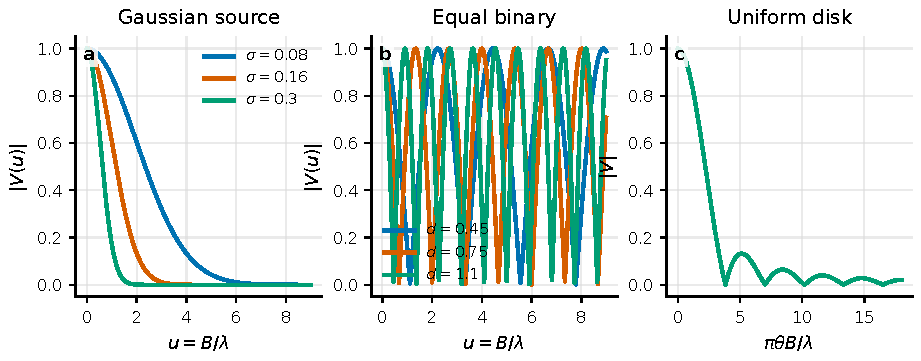
\includegraphics[width=0.9\linewidth]{figures/generated/chapter_01/ch01_fourier_visibility.pdf}
\caption{The normalized visibility \(|V|\) versus spatial frequency for several sky-brightness structures: a Gaussian source declines smoothly, equal-brightness binary stars produce cosine oscillations, and a uniform disk, because of its sharp edge, shows zeros and sidelobes. This is completely isomorphic to this chapter's temporal "spectral line shape \(\leftrightarrow\) fringe decay": the sinc sidelobes of a rectangular spectrum correspond to the Bessel sidelobes of a uniform disk; only the "frequency spectrum" is replaced by the "sky brightness distribution," and the "time delay" by the "spatial baseline."}
\label{fig:e09-fourier-visibility}
\end{figure}

This axis change is astonishingly powerful. The Wiener--Khinchin theorem says "\(g^{(1)}(\tau)\) is the Fourier transform of the power spectrum \(S(\nu)\)"; its spatial twin (the protagonist of the next chapter, the van Cittert--Zernike theorem) will say "\(\gamma_{12}\) is the Fourier transform of the sky brightness distribution \(I(l,m)\)." So every conclusion of this chapter has a spatial counterpart: the shape of the fringe decay tells us the spectral line shape, just as the shape of the visibility versus baseline tells us the \emph{source's angular structure}; the sinc sidelobes of a rectangular spectrum correspond to the Bessel sidelobes of a uniform disk (Fig.~\ref{fig:e09-fourier-visibility}); the coherence length \(\ell_c\) is to delay as some critical baseline is to angular scale. Shifting this whole intuition of temporal coherence over to space is our ticket into spatial coherence and imaging.

Carrying one sentence into the next chapter: \textbf{the visibility is the reading of first-order coherence, and first-order coherence gives the spectral line along the time axis and the image along the spatial baseline.} Chapter \ref{chap:e10} starts from \(\gamma_{12}\), uses the van Cittert--Zernike theorem to turn it into a Fourier component of the sky, and then uses intensity interferometry to measure \(|\gamma_{12}|^2\), stepping toward stellar angular diameters and imaging.

\section{Chapter Summary}
\label{sec:e09-summary}

\begin{itemize}
  \item \textbf{The fringe formula.} A two-path optical-path difference \(\Delta\) introduces the carrier phase \(\delta=2\pi\Delta/\lambda\) and time delay \(\tau=\Delta/c\), and the detected intensity is \(I(\delta)=I_1+I_2+2\sqrt{I_1I_2}\,|g^{(1)}(\tau)|\cos(\delta-\varphi(\tau))\), where \(\varphi(\tau)\) is the slow residual phase after removing the carrier (zero for a symmetric spectral line). The amplitude of the cosine term is proportional to the first-order degree of coherence \(|g^{(1)}|\).
  \item \textbf{The visibility is the reading of the degree of coherence.} \(\mathcal V=(I_{\max}-I_{\min})/(I_{\max}+I_{\min})=\dfrac{2\sqrt{I_1I_2}}{I_1+I_2}|g^{(1)}(\tau)|\); at equal intensity \(\mathcal V=|g^{(1)}(\tau)|\). The abstract "how much phase the field still remembers" becomes fringe contrast readable by eye.
  \item \textbf{Coherence length.} The fringes fade as the optical-path difference grows, with characteristic scale \(\ell_c=c\tau_c\simeq\lambda^2/\Delta\lambda\): about 1\,\(\mu\)m for white light, about 0.3\,mm for a 1\,nm narrowband, about 300\,m for a MHz laser.
  \item \textbf{The Wiener--Khinchin bridge.} \(g^{(1)}(\tau)\) is the Fourier transform of the normalized power spectrum; a rectangular spectrum gives \(|g^{(1)}|=|{\rm sinc}(\Delta\nu\tau)|\) (with zeros and sidelobes), a Lorentzian gives \(|g^{(1)}|=e^{-|\tau|/\tau_c}\) (pure exponential). Hence measuring the fringe decay with delay can infer the spectral line shape: the principle of Fourier-transform spectroscopy.
  \item \textbf{Two routes.} Amplitude interferometry directly measures the complex visibility (with phase) but requires the optical path stable to a fraction of a wavelength and is sensitive to atmospheric piston; intensity interferometry measures only \(|\mathcal V|^2\), losing phase, but needs only electronic alignment to a fraction of the response time (see the comparison table, leading into Chapter \ref{chap:e10}).
  \item \textbf{Change of axis to space.} Replace the time-delay version \(g^{(1)}(\tau)\) with the two-point spatial version \(\gamma_{12}\), with visibility \(\mathcal V=|\gamma_{12}|\); it is the protagonist of the next chapter's van Cittert--Zernike theorem and intensity interferometry.
\end{itemize}

\medskip
\noindent\textbf{Questions to Ponder.}
\begin{enumerate}
  \item A Michelson interferometer under white light shows colored fringes only when the two arms are almost equal in length; with a \(\Delta\lambda=1\,{\rm nm}\) narrowband filter, to how large does the allowed two-arm optical-path difference expand? Estimate using Eq.~\eqref{eq:e09-coherence-length}.
  \item The two path intensities are in the ratio \(I_1:I_2=4:1\); even if the light is fully coherent (\(|g^{(1)}|=1\)), what is the highest fringe visibility attainable? This shows that "not seeing full-amplitude fringes" need not mean incoherence.
  \item If the measured visibility decays as a pure exponential with delay, \(\mathcal V(\tau)=e^{-|\tau|/\tau_c}\), with \(\tau_c=1\,{\rm ns}\), what shape is the corresponding spectral line, and what is the linewidth \(\Delta\nu\)? Converted to wavelength, how "narrow" is this line?
\end{enumerate}

\chapter{Spatial Coherence, van Cittert--Zernike, and Intensity Interferometry}
\label{chap:e10}

\begin{chapteropening}
Chapter \ref{chap:e09} dealt with the "temporal version" of coherence: whether the same beam of light, at this instant and a little later, still remembers its own phase. This chapter moves the very same question into space. Imagine two telescopes, separated by tens of meters, hundreds of meters, or even kilometers, staring at once at the same star in the night sky. Is the light each receives "two small patches of the same wavefront"? If so, the two intensities brighten and dim together, their fluctuations synchronous; if this star subtends a large enough angle on the sky, then what the two telescopes sample are two already "offset" patches of the wavefront, their fluctuations going their separate ways, no longer synchronous. The marvel is that the degree of synchrony tells us directly how large this star is, even if, in the largest optical telescope, it is only a point. This chapter joins this chain link by link: first use pure geometry to compute "how fine an angular structure two telescopes see," then use the van Cittert--Zernike theorem to translate "what the sky looks like" into "the degree of coherence," and then, borrowing the Siegert relation of Chapter \ref{chap:e08}, explain why one can measure a star's size \emph{without combining the two beams, comparing only the jitter of their respective intensities}. Finally we will meet the weak spot of intensity interferometry (the phase is lost) and the benefit it buys in exchange: near-immunity to atmospheric jitter.
\end{chapteropening}

\section{Geometry: Two Telescopes, One Baseline, One Angular Scale}
\label{sec:e10-geometry}

Let us first set aside correlators, photons, and quantum statistics, and look at a single geometric fact, one that needs no camera at all, just a ruler and a little trigonometry.

Starlight from some direction in the sky, at a place far enough away, has had its wavefront flattened into an almost perfectly straight plane (this is the "far field"). Let the star's direction on the sky be specified by a unit vector \(\bm s\). Two telescopes stand at positions \(\bm x_1\) and \(\bm x_2\), and the vector joining them is called the \textbf{baseline}:
\[
  \bm B=\bm x_2-\bm x_1 .
\]
The same plane wavefront sweeps across one telescope first and then the other, traversing unequal path lengths. This \textbf{path difference} equals the length of the baseline projected onto the propagation direction of the starlight, that is, the dot product \(\bm B\cdot\bm s\). What truly matters for interference is the part of the baseline perpendicular to the line of sight, "lying on the plane of the sky," denoted the projected baseline \(\bm B_\perp\); the component along the line of sight merely makes the whole wavefront arrive earlier or later as a whole, without changing the transverse structure the two telescopes see.

Now focus on the fact that "the star is not a point, but a small patch of sky." Take the direction of the star's center as \(\bm s_0\), and in the \emph{local sky plane} perpendicular to the line of sight erect two orthogonal unit directions \(\hat{\bm e}_x,\hat{\bm e}_y\) (each aligned with the direction of one baseline component). Any point on the star's face, offset from the center by a small angle, is labeled by two small-angle coordinates \((l,m)\) marking this transverse offset (\(l,m\) both in radians, dimensionless, with typical values on the order of \(10^{-9}\) radians, i.e.\ milliarcseconds). Then this point's direction can be written
\[
  \bm s\approx\bm s_0+l\,\hat{\bm e}_x+m\,\hat{\bm e}_y ,
\]
where, to first order in the small angle, \(\bm s\) is still approximately normalized (the transverse offset changes \(|\bm s|\) only at second order \(\mathcal O(l^2,m^2)\), which is negligible). The extra path difference it brings, in the part that differs from the center, is
\[
  \Delta(\bm B\cdot\bm s)=B_x\,l+B_y\,m ,
\]
where \(B_x,B_y\) are the components of the projected baseline \(\bm B_\perp\) along the two orthogonal directions of the sky plane (in meters). The path difference divided by the wavelength \(\lambda\) and multiplied by \(2\pi\) is the phase difference this point brings to the two telescopes. So we naturally define a pair of \textbf{spatial frequencies}:

\begin{equation}
  u=\frac{B_x}{\lambda},\qquad v=\frac{B_y}{\lambda}.
  \label{eq:e10-uv}
\end{equation}
\begin{formulaexplain}
\(B_x,B_y\): the components of the projected baseline along the two directions of the sky plane (meters). \(\lambda\): the observation wavelength (meters). \(u,v\): the spatial frequencies measured in "numbers of wavelengths," dimensionless. The same baseline at a shorter wavelength samples finer angular structure.
\end{formulaexplain}

Why call it "spatial frequency" rather than simply "resolution"? Because \(u,v\) count "how many fringes fit into one wavelength across this baseline." It is a sampling coordinate on the Fourier plane, not the angular resolution itself. Let us substitute real numbers to feel it: take \(B=100\,\mathrm{m}\), \(\lambda=500\,\mathrm{nm}=5\times10^{-7}\,\mathrm{m}\),
\[
  \frac{B}{\lambda}=\frac{100}{5\times10^{-7}}=2\times10^{8}.
\]
Two hundred million: this is a pure number, meaning this baseline spans two hundred million wavelengths. To get the angular scale, one must \emph{invert} it:
\[
  \frac{\lambda}{B}=\frac{1}{2\times10^{8}}=5\times10^{-9}\ \mathrm{rad}.
\]
Convert radians to milliarcseconds (\(1\,\mathrm{mas}=4.848\times10^{-9}\,\mathrm{rad}\)):
\[
  5\times10^{-9}\,\mathrm{rad}=\frac{5\times10^{-9}}{4.848\times10^{-9}}\,\mathrm{mas}\approx1.0\,\mathrm{mas}.
\]
So a hundred-meter baseline, in blue-green light, innately corresponds to about 1 milliarcsecond of angular scale, already tens of times finer than the best single-aperture telescope (diffraction limit of tens of milliarcseconds). This is the whole allure of interferometry: the resolving power is set by the \emph{distance between telescopes}, not by the mirror aperture.

\section{First-Order Spatial Coherence: a Complex Arrow Across Telescopes}
\label{sec:e10-gamma12}

Geometry tells us "how fine an angular structure this baseline corresponds to," but not "whether this star is actually resolved at that angular scale." To answer the latter, we must compare the fields the two telescopes actually receive.

Recall Chapter \ref{chap:e01}: the light field at a point at a given instant can be written as an arrow rotating in the complex plane, the complex amplitude \(\mathcal E\), whose length is the amplitude and whose angle is the phase. Now the two telescopes each have an arrow, \(E_1(t)\) and \(E_2(t)\). To ask "how in step they are," the most natural quantity is to conjugate one arrow, multiply it by the other, take the time average, and normalize by each one's own intensity. This quantity is called the \textbf{first-order spatial coherence} (also called the complex visibility):

\begin{equation}
  \gamma_{12}^{(1)}
  =\frac{\big\langle E_1^{\ast}(t)\,E_2(t)\big\rangle}
        {\sqrt{\big\langle|E_1(t)|^2\big\rangle\,\big\langle|E_2(t)|^2\big\rangle}} .
  \label{eq:e10-gamma12}
\end{equation}
\begin{formulaexplain}
\(E_1,E_2\): the complex fields received by the two telescopes. The numerator \(\langle E_1^{\ast}E_2\rangle\) is the "cross-telescope field correlation," and the denominator normalizes by the square root of each one's mean intensity. The result \(\gamma_{12}^{(1)}\) is complex: the modulus \(|\gamma_{12}^{(1)}|\in[0,1]\) gives the coherence strength, and the argument gives the Fourier phase.
\end{formulaexplain}

Let us spell out each symbol. \(E_1(t),E_2(t)\): the complex amplitudes of the electric field received by the two telescopes at the same instant (in CGS the dimensions are \(\mathrm{statvolt\,cm^{-1}}\), but after normalization the units all cancel). The angle brackets \(\langle\cdot\rangle\) are the long-time average over time. In the denominator, \(\langle|E_1|^2\rangle\) is proportional to the mean intensity of the first telescope; taking the square root and multiplying by the second's exactly divides out the absolute scale of both intensities, so \(\gamma_{12}^{(1)}\) reflects only the "step," independent of which telescope collects more and which less.

Why use a complex number rather than a single real one? Because "being in step" itself carries two layers of information: \emph{how much in step} (modulus) and \emph{how much the phase has shifted} (argument). An amplitude interferometer (the kind of instrument in Chapter \ref{chap:e09} that combines the two beams via a delay line to view fringes) can read both the modulus and the argument of this complex arrow: the fringe contrast gives the modulus, the fringe position gives the argument. But the intensity interferometer to be discussed later in this chapter does \emph{not} combine beams in optics; it compares, after detection, the jitter of the two intensities, and in the end obtains only \(|\gamma_{12}^{(1)}|^2\), the argument lost. This "loss of phase" is the core feature of intensity interferometry, and we settle the account in Section \ref{sec:e10-phase}.

So what determines \(\gamma_{12}^{(1)}\)? The next section's van Cittert--Zernike theorem gives an astonishingly clean answer: it is the Fourier transform of the sky brightness distribution.

\section{The van Cittert--Zernike Theorem: the Look of the Sky Determines the Degree of Coherence}
\label{sec:e10-vcz}

Now for the most crucial derivation of this chapter. We will prove: for a "distant, internally incoherent" source, the spatial degree of coherence \(\gamma_{12}^{(1)}\) between two telescopes is exactly the \emph{normalized Fourier component} of the sky brightness distribution. This conclusion is called the van Cittert--Zernike theorem (VCZ for short), and it is the foundation of all interferometric imaging \citep{1938Phy.....5..785Z,1939Phy.....6.1129V}.

\textbf{The physical picture first.} Think of the star's face as a densely packed multitude of independent little light bulbs, each bulb in a direction \((l,m)\) with brightness \(I_\nu(l,m)\). "Internally incoherent" (spatially incoherent) means: the emissions of any two different bulbs have no phase relationship whatsoever: they are each independent thermal-radiation sources with random phase. The key is: the plane wave emitted by the \emph{same bulb} is completely coherent at the two telescopes (the same wavefront); it is only that different bulbs, because of their different directions, bring \emph{different phase differences} to the two telescopes.

\textbf{Step-by-step derivation.} To spell it out so that "the reader need supply no step," let us write the field out explicitly. The complex field received by the \(j\)-th telescope (\(j=1,2\)) is the superposition of the contributions of the bulbs in all sky directions:

\[
  E_j(t)=\int\sqrt{I_\nu(l,m)}\;a(l,m,t)\;
  \exp\!\big[-2\pi i\,(u_j\,l+v_j\,m)\big]\,\mathrm dl\,\mathrm dm .
\]

Here \(\sqrt{I_\nu(l,m)}\) is the amplitude scale of the bulb in direction \((l,m)\) (the square root of the brightness); \(a(l,m,t)\) is that bulb's \emph{complex random amplitude}: it packs in the randomly jittering phase and amplitude of the thermal-radiation source, and is a zero-mean random quantity; the exponential \(\exp[-2\pi i(u_j l+v_j m)]\) is the geometric phase of this bulb's plane wave, relative to the central direction, as it sweeps to the \(j\)-th telescope, where \((u_j,v_j)=(B_{x,j},B_{y,j})/\lambda\) is set by that telescope's position (citing the path-difference phase \(2\pi(ul+vm)\) of Section \ref{sec:e10-geometry}).

In computing the cross-telescope field correlation \(\langle E_1^{\ast}(t)E_2(t)\rangle\), multiplying the two integrals produces cross terms of all pairwise bulb pairings. To avoid confusion with the integration variables, denote the first telescope's direction as \((l_a,m_a)\) and the second's as \((l_b,m_b)\):

\[
  \big\langle E_1^{\ast}(t)E_2(t)\big\rangle
  =\int\!\!\int
  \sqrt{I_\nu(l_a,m_a)\,I_\nu(l_b,m_b)}\;
  \big\langle a^{\ast}(l_a,m_a,t)\,a(l_b,m_b,t)\big\rangle\;
  e^{\,2\pi i(u_1 l_a+v_1 m_a)}\,e^{-2\pi i(u_2 l_b+v_2 m_b)}\,
  \mathrm d\Omega_a\,\mathrm d\Omega_b ,
\]

where \(\mathrm d\Omega=\mathrm dl\,\mathrm dm\). Now invoke the \emph{incoherence condition} (the algebraic form of "independent random phases"): bulbs in different directions are mutually independent and each random, so the correlation of their complex amplitudes is nonzero only for the \emph{same bulb},

\[
  \big\langle a^{\ast}(l_a,m_a,t)\,a(l_b,m_b,t)\big\rangle
  =\delta(l_a-l_b)\,\delta(m_a-m_b) ,
\]

that is, the cross terms with \(a\neq b\) are smeared to zero by random-phase averaging (\(\langle a_a^\ast a_b\rangle=0\)), and only the diagonal terms \(a=b\) survive. Substituting this \(\delta\) function uses up the second set of integrals, setting \((l_b,m_b)=(l_a,m_a)\), and the two geometric phases combine into a \emph{difference}: \(e^{2\pi i(u_1 l+v_1 m)}e^{-2\pi i(u_2 l+v_2 m)}=e^{-2\pi i[(u_2-u_1)l+(v_2-v_1)m]}\). Denoting the spatial frequency given by the baseline difference as \((u,v)=(u_2-u_1,\,v_2-v_1)\) (exactly the \(u,v\) corresponding to the baseline \(\bm B=\bm x_2-\bm x_1\) of Section \ref{sec:e10-geometry}), we have

\[
  \big\langle E_1^{\ast}(t)E_2(t)\big\rangle
  =\int I_\nu(l,m)\,\exp\!\big[-2\pi i\,(u\,l+v\,m)\big]\,\mathrm dl\,\mathrm dm .
\]

Finally normalize by the two mean intensities per the definition Eq.~\eqref{eq:e10-gamma12}. In the denominator \(\langle|E_j|^2\rangle=\int I_\nu\,\mathrm dl\,\mathrm dm\) (for the same telescope, \(u_j=v_j\) cancel, the geometric phase is gone, and the total flux remains), the same for both telescopes, so after taking the square root it is still this total flux. Dividing numerator and denominator by the same, we obtain

\begin{equation}
  \gamma^{(1)}(u,v)
  =\frac{\displaystyle\int I_\nu(l,m)\,\exp\!\big[-2\pi i\,(u\,l+v\,m)\big]\,\mathrm dl\,\mathrm dm}
        {\displaystyle\int I_\nu(l,m)\,\mathrm dl\,\mathrm dm}.
  \label{eq:e10-vcz}
\end{equation}
\begin{formulaexplain}
Numerator: multiply the sky brightness \(I_\nu(l,m)\) by the geometric phase factor and integrate over the whole star's face: this is a two-dimensional Fourier transform. Denominator: the total flux, used to set \(\gamma^{(1)}(0,0)\) to 1. The conclusion in one sentence: \emph{the degree of coherence is the normalized Fourier component of the sky}.
\end{formulaexplain}

Let us bring each symbol down to earth. \(I_\nu(l,m)\): the specific intensity in direction \((l,m)\), commonly in units of \(\mathrm{erg\,s^{-1}\,cm^{-2}\,Hz^{-1}\,sr^{-1}}\), which can also be understood as "how bright it is per direction, per hertz of bandwidth." \(l,m\): small-angle coordinates (radians). In the exponential, \(u,l\) and \(v,m\) are paired, exactly the spatial frequency of Eq.~\eqref{eq:e10-uv} times the small angle, a pure phase, dimensionless. The denominator adds up all the star's light into the total flux, and dividing it out ensures that at zero baseline (\(u=v=0\), the two telescopes side by side) \(\gamma^{(1)}(0,0)=1\), i.e.\ "fully coherent."

The physical meaning of this formula deserves repeated savoring: \textbf{short baselines see coarse structure, long baselines see fine structure.} When \(u,v\) are small (baseline short), the phase factor barely changes over the whole star's face, the integral is approximately the total flux, and \(\gamma^{(1)}\approx1\): two telescopes close together are of course in step, because they sample the same small patch of the wavefront. As \(u,v\) grow (baseline lengthened), the phase factor begins to turn round and round over the star's face, positives and negatives cancel, the integral shrinks, and \(\gamma^{(1)}\) drops: this shows the star has been "resolved" at this angular scale. So \emph{how fast the degree of coherence drops with baseline encodes the star's size and shape}.

\textbf{Conditions of validity (check again if you cross them).} Equation~\eqref{eq:e10-vcz} is not unconditional; it used four premises, none of which may be missing:
\begin{itemize}
  \item \textbf{Source internally incoherent}: the emission phases of different points on the star's face are mutually independent; the "random-phase averaging" step above rests on this. Thermal-radiation objects almost always satisfy it.
  \item \textbf{Narrowband}: the bandwidth must be narrow, or else different wavelengths \(\lambda\) give different \(u,v\) (see Eq.~\eqref{eq:e10-uv}), smearing different spatial frequencies together.
  \item \textbf{Small field of view}: the star's subtended angle is small enough that one may use the plane \((l,m)\) coordinates and linear phase, neglecting the second-order term along the line of sight (called the \(w\)-term in radio).
  \item \textbf{Source invariant}: over the time the correlation is accumulated, the star's structure must not change significantly, or else what is averaged is something in motion.
\end{itemize}
For ordinary thermal stars and narrowband blue light in intensity interferometry, these four are generally well satisfied; but for fast transients, broadband imaging, and large-field targets, one must recheck them one by one \citep{1938Phy.....5..785Z,1939Phy.....6.1129V}.

\begin{figure}[tbp]
\centering
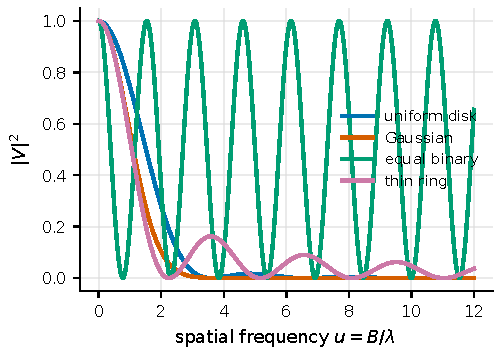
\includegraphics[width=0.88\linewidth]{figures/generated/chapter_05/ch05_vcz_visibility_models.pdf}
\caption{Different sky-brightness models leave different fingerprints on the squared visibility \(|V|^2\). A uniform disk shows Bessel-type zeros, a Gaussian source decays smoothly, equal-brightness binary stars superpose a layer of cosine oscillation, and a thin ring gives denser oscillation. What intensity interferometry directly measures is precisely these curves (their squared modulus), so "reading the curve" amounts to "guessing what the sky looks like."}
\label{fig:e10-vcz-models}
\end{figure}

\section{The Uniform Disk: Measuring a Stellar Angular Diameter from One Curve}
\label{sec:e10-disk}

The VCZ theorem gives the general formula, but the sky comes in a thousand shapes. To truly master it, one must practice on the cleanest model: the \textbf{uniform disk}. Assume the star is a circular face of angular diameter \(\theta\), with equal surface brightness everywhere inside the circle and zero outside. This is the approximation of "treating the star as a uniformly glowing coin."

\textbf{Deriving the visibility.} For a circularly symmetric brightness distribution, the two-dimensional Fourier transform degenerates into a one-dimensional Hankel transform. Let the disk radius (angular radius) be \(a=\theta/2\), and the radial spatial frequency \(q=B/\lambda\). For circular symmetry the numerator of Eq.~\eqref{eq:e10-vcz} is written
\[
  \int_0^{a} I_0\,J_0(2\pi q r)\,2\pi r\,\mathrm dr
  =2\pi I_0\int_0^{a}J_0(2\pi q r)\,r\,\mathrm dr,
\]
where \(J_0\) is the zeroth-order Bessel function, the "circularly symmetric cosine," which is exactly what remains after integrating the two-dimensional phase factor once around the circle. Here we use a standard Bessel integral identity (found in any handbook of mathematical physics):
\[
  \int_0^{a} J_0(k r)\,r\,\mathrm dr=\frac{a}{k}\,J_1(k a),
\]
taking \(k=2\pi q\). The denominator is the disk's total flux \(I_0\cdot\pi a^2\). Dividing the two:
\[
  \gamma^{(1)}
  =\frac{2\pi I_0\cdot\dfrac{a}{2\pi q}J_1(2\pi q a)}{I_0\,\pi a^2}
  =\frac{2\,J_1(2\pi q a)}{2\pi q a}.
\]
Denoting the dimensionless combination \(x\equiv 2\pi q a=2\pi\dfrac{B}{\lambda}\cdot\dfrac{\theta}{2}=\dfrac{\pi\theta B}{\lambda}\), we obtain that famous curve:

\begin{equation}
  V(B)=\frac{2\,J_1(x)}{x},\qquad x=\frac{\pi\,\theta\,B}{\lambda}.
  \label{eq:e10-disk}
\end{equation}
\begin{formulaexplain}
\(V(B)\): the visibility of a uniform disk on baseline \(B\). \(J_1\): the first-order Bessel function. \(x=\pi\theta B/\lambda\): the dimensionless "degree of resolution": the larger it is, the more the star is spread apart. As \(x\to0\), \(2J_1(x)/x\to1\) (not resolved at all).
\end{formulaexplain}

Let us account for each symbol. \(V(B)\): the visibility, dimensionless, which is the \(\gamma^{(1)}\) on this baseline (real for a disk). \(J_1(x)\): the first-order Bessel function; here we \emph{explicitly cite} this known result: the Fourier transform of a circular aperture always gives a \(J_1\)-type pattern, of the same origin as the Airy pattern of a circular hole in optics. \(\theta\): the angular diameter (radians); \(B\): the projected baseline (meters); \(\lambda\): the wavelength (meters). Most important is that combination \(x=\pi\theta B/\lambda\): for the same star, the longer the baseline or the shorter the wavelength, the larger \(x\) and the more easily resolved; for the same baseline, the larger the star, the larger \(x\) and the more sensitive.

\textbf{The first zero.} The curve \(2J_1(x)/x\) first falls to zero at the first nonzero root of \(J_1(x)=0\). This root is a known number: \(x=3.8317\). Setting \(\pi\theta B_0/\lambda=3.8317\) solves for the critical baseline:
\[
  B_0=\frac{3.8317}{\pi}\cdot\frac{\lambda}{\theta}=1.2197\,\frac{\lambda}{\theta}\approx1.22\,\frac{\lambda}{\theta}.
\]

\begin{equation}
  B_0\approx\frac{1.22\,\lambda}{\theta}.
  \label{eq:e10-null}
\end{equation}
\begin{formulaexplain}
\(B_0\): the baseline (meters) at which the visibility first drops to zero. \(\lambda\): wavelength, \(\theta\): angular diameter. It marks the telescope separation needed to "just resolve the star to the first dark fringe," looking exactly like the single-aperture diffraction limit \(1.22\lambda/D\), only with the aperture \(D\) replaced by the baseline \(B\).
\end{formulaexplain}

\textbf{Substituting real numbers.} Take the blue light \(\lambda=416\,\mathrm{nm}\) commonly used by VERITAS and MAGIC, and see how long a baseline several stellar sizes require:
\[
  \theta=0.5\,\mathrm{mas}=0.5\times4.848\times10^{-9}\,\mathrm{rad}=2.424\times10^{-9}\,\mathrm{rad},
\]
\[
  B_0=1.22\times\frac{416\times10^{-9}}{2.424\times10^{-9}}
  =1.22\times171.6\,\mathrm{m}\approx210\,\mathrm{m}.
\]
Similarly, \(\theta=1\,\mathrm{mas}\) needs only about \(105\,\mathrm{m}\), and \(\theta=0.2\,\mathrm{mas}\) needs about \(520\,\mathrm{m}\). These few numbers explain the whole span of instrument history: the Narrabri intensity interferometer used a variable baseline of 10--188 m, enough to measure those brighter, sub-milliarcsecond stars; but to reach down to tens of microarcseconds, one must go to kilometer-scale baselines, which is exactly the motivation for using atmospheric Cherenkov telescope arrays (VERITAS, MAGIC, the future CTAO) as intensity interferometers \citep{1967MNRAS.137..375H,2020NatAs...4.1164A}.

\begin{figure}[tbp]
\centering
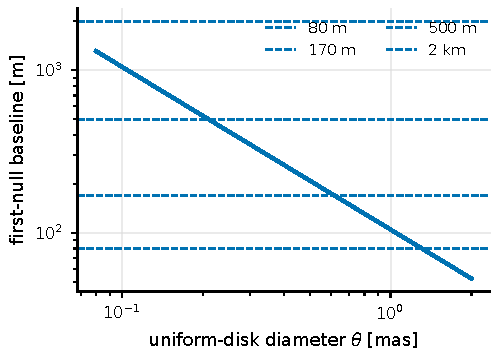
\includegraphics[width=0.86\linewidth]{figures/generated/chapter_05/ch05_uniform_disk_resolution.pdf}
\caption{The first-zero baseline of a uniform disk at \(\lambda=416\,\mathrm{nm}\) versus angular diameter. A 0.5 mas star needs about 210 m to reach its first zero, while a target of order 0.1 mas requires kilometer-scale baselines: this is why long-baseline Cherenkov arrays are so attractive for blue-light intensity interferometry.}
\label{fig:e10-disk-resolution}
\end{figure}

A practical reminder: what carries the most information in observing is often \emph{not} the zero itself, but the "descending region" before the zero. At short baselines, the curves of various angular diameters all cling to \(|V|^2\approx1\), indistinguishable; after the zero, \(|V|^2\) is too low, and systematic errors and background easily drown the signal; only the descending region has both appreciable signal and sensitivity to \(\theta\). So the first thing in designing an observation is to plot the \(|V(B)|^2\) of the target model and let the baselines cover this descending region (see Fig.~\ref{fig:e10-vcz-models}).

\section{Spatial HBT: No Beam Combining, Just Whether Intensity Jitter Is Synchronous}
\label{sec:e10-hbt}

Up to here we have kept talking about first-order coherence \(\gamma^{(1)}\) and the complex visibility: that is what an amplitude interferometer measures, requiring the two beams to be carefully combined in optics. Intensity interferometry takes another route: it does not combine beams at all, and only after detection compares whether the jitter of the two \emph{intensities} is synchronous. On what grounds can this too measure \(|V|\)? The answer is the Siegert relation of Chapter \ref{chap:e08}.

In Chapter \ref{chap:e08} we established, for the same light path at different instants, \(g^{(2)}=1+\zeta|g^{(1)}|^2\): the intensity of thermal (chaotic) light clumps together (photon bunching), and the strength of the bunching is proportional to the squared modulus of the first-order degree of coherence. This relation holds just as well for "two light paths, same instant," as long as the time channel is replaced by the spatial channel:

\begin{equation}
  g_{12}^{(2)}(0)-1=\zeta\,\big|\gamma_{12}^{(1)}\big|^2=\zeta\,\big|V(B)\big|^2 .
  \label{eq:e10-siegert}
\end{equation}
\begin{formulaexplain}
\(g_{12}^{(2)}(0)-1\): the "excess" of the zero-delay intensity correlation of the two telescopes (the extra clumping relative to accidental coincidence). \(\zeta\): the dilution factor (time response, bandwidth, polarization, and background together lower the bunching height). \(|V(B)|^2\): the squared visibility, exactly the celestial structure we want.
\end{formulaexplain}

Let us explain each symbol. \(g_{12}^{(2)}(0)\): the normalized second-order correlation of the two intensities at zero time delay; subtracting 1 gives the excess relative to the "completely random, uncorrelated" baseline. \(\zeta\) (dimensionless, between 0 and 1): bundles in everything that "flattens the bunching peak": the finite detector time width, the finite optical bandwidth, unselected polarization, background-light dilution. \(|\gamma_{12}^{(1)}|^2\): for thermal light / Gaussian chaotic light, it equals \(|V(B)|^2\). This formula is the heart of spatial HBT (Hanbury Brown--Twiss): \textbf{the degree of synchrony of the intensity jitter of the two telescopes directly gives the squared visibility}, with no beam combining anywhere \citep{1956Natur.177...27B}.

\textbf{The observation model.} On a real machine, data analysis often writes Eq.~\eqref{eq:e10-siegert} as a model that separates the three things "instrument, background, celestial object." This step is really just \emph{writing out clearly the lumped dilution factor \(\zeta\) of Eq.~\eqref{eq:e10-siegert}}, splitting it into \(\zeta=N_0\,f_1 f_2\): \(N_0\) collects the instrument-side dilution (detector time response, bandwidth, polarization, i.e.\ the term Eq.~\eqref{eq:e10-n0} below), and \(f_1 f_2\) collects the background-side dilution (the fraction of target photons out of the total counts of the two telescopes). So the dilution factor has not vanished; it is only split into "instrument \(\times\) background," each of which can be calibrated separately:

\begin{equation}
  C_{12}(B)\equiv g_{12}^{(2)}(0)-1=N_0\,f_1 f_2\,\big|V(B)\big|^2 .
  \label{eq:e10-model}
\end{equation}
\begin{formulaexplain}
\(C_{12}\): the measured correlation-peak height. \(N_0\): the zero-baseline instrument response (the bunching height that should occur when the star is not spatially resolved). \(f_1,f_2\): the fractions of target photons out of the total counts in the two telescopes. \(|V|^2\): the celestial structure term. The product of the three cleanly separates instrument, background, and sky.
\end{formulaexplain}

Symbol by symbol: \(C_{12}(B)\) is the correlation-peak amplitude on baseline \(B\) (dimensionless); \(N_0\) is the \emph{zero-baseline} correlation amplitude, i.e.\ the bunching height that should occur when the two telescopes are side by side and the star is completely unresolved (\(|V|=1\)), which collects in all the post-detection instrument effects; \(f_1,f_2\) (dimensionless, \(\le1\)) are the fractions of light truly from the target in each telescope: moonlight, night-sky light, and neighboring stars pull it down; \(V(B)\) is the normalized visibility given by Eq.~\eqref{eq:e10-disk} (or a more complex model). This product structure lets the analysis be calibrated term by term: \(|V|^2\) varies with baseline, \(f_1f_2\) varies with background, and \(N_0\) is the instrument's "identity card."

\textbf{How small is the zero-baseline amplitude.} For unpolarized thermal light, if the detector has an effective time width \(\Delta t_{\rm eff}\) and an optical bandwidth \(\Delta\nu\), the order of magnitude of the zero-baseline amplitude is

\begin{equation}
  N_0\sim\frac{1}{2\,\Delta\nu\,\Delta t_{\rm eff}},\qquad
  \Delta\nu\simeq\frac{c\,\Delta\lambda}{\lambda^2}.
  \label{eq:e10-n0}
\end{equation}
\begin{formulaexplain}
\(N_0\): the bunching-peak height when the star is unresolved. \(\Delta\nu\): the optical frequency bandwidth (Hz). \(\Delta t_{\rm eff}\): the electronic effective time width (s). The \(2\) in the denominator is the dilution from unselected polarization (two polarization modes). The wider the bandwidth and the slower the time response, the lower the thermal-light bunching peak is averaged down.
\end{formulaexplain}

Physically this is easy to understand (recall from Chapter \ref{chap:e02} that bandwidth and coherence time are reciprocals): bunching is only "visible" within one coherence time \(\tau_c\sim1/\Delta\nu\), while the detector must spend \(\Delta t_{\rm eff}\) integrating. When the detector is much slower than the coherence time (\(\Delta t_{\rm eff}\gg\tau_c\)), a single integration packs in \(\sim\Delta t_{\rm eff}/\tau_c=\Delta\nu\,\Delta t_{\rm eff}\) mutually uncorrelated coherence blocks, and the bunching signal is thinned by averaging over so many blocks, so \(N_0\) is inversely proportional to this large number.

\textbf{Substituting VERITAS's real parameters} (\(\lambda=416\,\mathrm{nm}\), \(\Delta\lambda=13\,\mathrm{nm}\), \(\Delta t_{\rm eff}\sim4\,\mathrm{ns}\)): first compute the bandwidth
\[
  \Delta\nu\simeq\frac{c\,\Delta\lambda}{\lambda^2}
  =\frac{(3\times10^8)\,(13\times10^{-9})}{(416\times10^{-9})^2}
  =\frac{3.9}{1.73\times10^{-13}}\ \mathrm{Hz}\approx2.3\times10^{13}\,\mathrm{Hz},
\]
then substitute into \(N_0\):
\[
  N_0\sim\frac{1}{2\,(2.3\times10^{13})\,(4\times10^{-9})}
  =\frac{1}{1.8\times10^{5}}\approx5\times10^{-6}.
\]
The order of magnitude is a few parts per million. The \(N_0\approx1.25\times10^{-6}\) obtained by fitting the real machine is slightly lower than the crude estimate, because the real filter shape, electronic response, and system efficiency further suppress the peak. In any case, the conclusion is sobering: \textbf{the bunching peak of thermal light is only of order one part in a million}, and to measure a star on such a low signal relies on long-duration accumulation and stringent calibration of \(N_0\) (Fig.~\ref{fig:e10-zero-baseline}) \citep{2020NatAs...4.1164A}.

\begin{figure}[tbp]
\centering
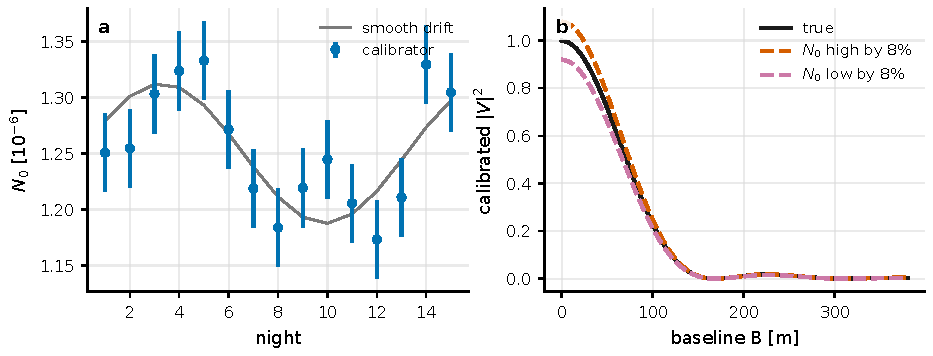
\includegraphics[width=0.92\linewidth]{figures/generated/chapter_05/ch05_zero_baseline_calibration.pdf}
\caption{The calibration of the zero-baseline amplitude \(N_0\) carries directly over onto \(|V|^2\). Left: the nightly \(N_0\) drift given by calibration stars. Right: if \(N_0\) is 8\% too high or too low, \emph{all} baselines' \(|V|^2\) are stretched as a whole, pushing the fits of angular diameter, limb darkening, or oblateness toward wrong values. This explains why \(N_0\) is the most critical systematic in intensity interferometry.}
\label{fig:e10-zero-baseline}
\end{figure}

\section{Missing Phase: a Weak Spot, and Also an Amulet}
\label{sec:e10-phase}

Intensity interferometry measures only \(|V|^2\) (that squared modulus in Eq.~\eqref{eq:e10-model}), throwing away the argument (Fourier phase) of the complex visibility \(\gamma_{12}^{(1)}\). This brings an ambiguity of principle.

\textbf{Mirror degeneracy.} Consider a brightness distribution \(I(l,m)\) and its mirror image \(I(-l,-m)\), flipped about the center. Taking the Fourier transform per Eq.~\eqref{eq:e10-vcz}, the Fourier transform of a real brightness distribution satisfies \(\gamma(-u,-v)=\gamma^{\ast}(u,v)\) (because \(I\) is real); and the Fourier transform of the mirror distribution is exactly the complex conjugate of the original. Taking the squared modulus, complex conjugation does not change the modulus, so
\[
  \big|V_{\text{original}}(u,v)\big|^2=\big|V_{\text{mirror}}(u,v)\big|^2 .
\]
Two skies that look different give \emph{exactly the same} \(|V|^2\): an instrument that measures only the squared modulus cannot distinguish them (Fig.~\ref{fig:e10-phase-ambiguity}). This is why "imaging directly from \(|V|^2\)" is a hard matter requiring extra information (two-dimensional \(u,v\) coverage, physical priors, third-order correlation, or phase-retrieval algorithms), and we leave true imaging to Chapter \ref{chap:e11}.

\begin{figure}[tbp]
\centering
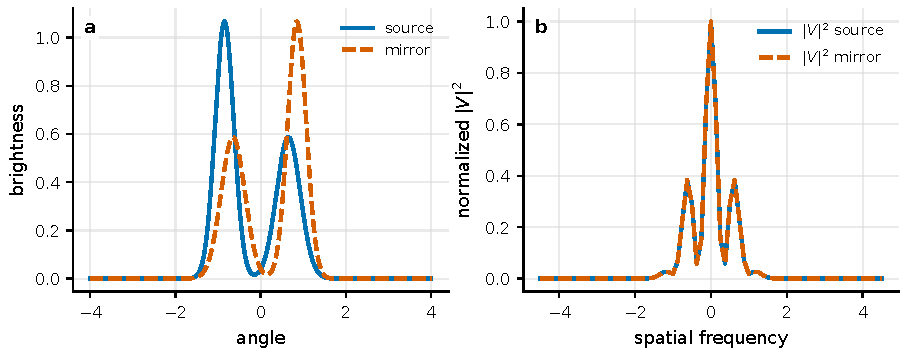
\includegraphics[width=0.92\linewidth]{figures/generated/chapter_05/ch05_phase_ambiguity.pdf}
\caption{Measuring only \(|V|^2\) loses the Fourier phase. Left: a source and its mirror source, with clearly different brightness distributions. Right: the \(|V|^2\) of the two coincide completely. To image, intensity interferometry must break such degeneracies through two-dimensional \(u,v\) coverage, physical priors, third-order (closure) correlation, or phase-retrieval algorithms.}
\label{fig:e10-phase-ambiguity}
\end{figure}

\textbf{What does losing the phase buy?} The answer is: near-immunity to optical path and atmospheric jitter, which is exactly the fundamental reason Cherenkov telescopes can do interferometry. An amplitude interferometer must combine the two beams in optics to view fringes, and so must stabilize the \emph{optical path} of the two light paths to a small fraction of a wavelength (of order tens of nanometers); but atmospheric turbulence makes the wavefront fluctuate ceaselessly, adding to each telescope a random, fast-jittering optical-path offset, termed the \textbf{piston phase}. Piston is fatal to amplitude interferometry, jittering the fringes away.

Intensity interferometry, however, hardly cares about it. The reason is: it compares whether the jitter of the two \emph{intensities} is synchronous, needing only to align the two \emph{electrical signals} in time to a small fraction of the detection response time. For a \(1\,\mathrm{GHz}\) electronic bandwidth, the time resolution is about 1 ns, and the corresponding optical-path tolerance is \(c\times1\,\mathrm{ns}\approx30\,\mathrm{cm}\): a path error of centimeters to tens of centimeters would be needed to noticeably reduce the correlation. Atmospheric piston's nanometer-to-micron optical-path jitter is not even a fraction of this tolerance. In other words, \textbf{intensity interferometry, at the cost of "losing the phase," buys the huge convenience of "not fearing the atmosphere and not needing precise optical path."} For exactly this reason, Cherenkov telescopes, whose optical image quality is far below that of professional interferometers but which have large apertures and fast detectors, turn out to be ideal intensity-interferometry arrays \citep{2006ApJ...649..399L,2024MNRAS.529.4387A}.

\section{Chapter Summary}
\label{sec:e10-summary}

\begin{itemize}
  \item \textbf{Geometry sets the angular scale.} The projected baseline \(\bm B_\perp\) gives the path difference \(\bm B\cdot\bm s\), and the spatial frequencies \(u=B_x/\lambda,\ v=B_y/\lambda\) are dimensionless "numbers of wavelengths." A hundred-meter baseline in blue-green light corresponds to about 1 mas (\(B/\lambda=2\times10^8\), inverted \(\lambda/B\approx1\,\mathrm{mas}\)). The resolving power is set by the baseline, not the aperture.
  \item \textbf{The degree of coherence is a complex arrow.} The first-order spatial degree of coherence \(\gamma_{12}^{(1)}=\langle E_1^\ast E_2\rangle/\sqrt{\langle|E_1|^2\rangle\langle|E_2|^2\rangle}\): the modulus gives the coherence strength, the argument gives the Fourier phase.
  \item \textbf{The van Cittert--Zernike theorem.} The \(\gamma^{(1)}(u,v)\) of an incoherent far-field source is the Fourier component of the normalized sky brightness (Eq.~\eqref{eq:e10-vcz}). Short baselines see coarse structure, long baselines see fine structure. Four conditions for validity: source internally incoherent, narrowband, small field of view, source invariant.
  \item \textbf{The uniform disk.} \(V(B)=2J_1(x)/x,\ x=\pi\theta B/\lambda\) (first-order Bessel function); the first zero \(x=3.8317\) gives \(B_0\approx1.22\lambda/\theta\). 416 nm, 0.5 mas \(\Rightarrow\) about 210 m. The most informative is the descending region before the zero.
  \item \textbf{Spatial HBT.} Carry the Siegert relation of Chapter \ref{chap:e08} over to the spatial channel: \(g_{12}^{(2)}(0)-1=\zeta|V(B)|^2\); no beam combining, just the synchrony of intensity jitter measures \(|V|^2\). The observation model \(C_{12}=N_0 f_1 f_2|V|^2\), zero-baseline amplitude \(N_0\sim1/(2\Delta\nu\Delta t_{\rm eff})\); VERITAS parameters give about \(5\times10^{-6}\), measured \(1.25\times10^{-6}\).
  \item \textbf{Missing phase is a double-edged sword.} Measuring only \(|V|^2\), the mirror brightness distribution \(I(-l,-m)\) gives the same \(|V|^2\) (degeneracy); but the price buys immunity to optical path / atmospheric piston, which is exactly why Cherenkov telescopes can do interferometry. Imaging is left to Chapter \ref{chap:e11}.
\end{itemize}

\medskip
\noindent\textbf{Questions to Ponder.}
\begin{itemize}
  \item If the observation wavelength is changed from 416 nm to the red light of 640 nm, will the first-zero baseline of the same 0.5 mas star become longer or shorter? To how many meters?
  \item If the target-photon fraction in the two telescopes drops from 70\% to 50\%, to what fraction of its original value is the correlation peak in Eq.~\eqref{eq:e10-model} suppressed? To recover the same significance, by roughly how many times must the integration time be increased (recall SNR grows only as the square root of time)?
  \item Why is "narrowband" a necessary condition of the VCZ theorem? If the bandwidth is very wide, what goes wrong with Eq.~\eqref{eq:e10-uv}?
\end{itemize}

\chapter{From Visibility to Imaging: Angular Diameters, Multiple Baselines, and uv Coverage}
\label{chap:e11}

\begin{chapteropening}
In the previous chapter we linked two far-separated telescopes together and proved that whether their recorded intensity fluctuations are synchronous directly gives the object's squared visibility on some baseline, \(|V(B)|^2\), a pure number between 0 and 1. But what an astronomer wants has never been a single number; it is "how big is this star," "is it round or flattened," "is it one star or two stuck together," "are there bright spots on its surface," and ultimately even a \emph{picture}. What this chapter does is turn that lone \(|V|^2\) on a single baseline, step by step, into a real scientific product: first work out clearly "how bright a star, how large a mirror, how long an exposure it takes to measure this number" (signal-to-noise ratio); then learn to judge "whether tonight's correlation peak is a real signal or the instrument playing tricks" (feasibility and error); then expand two telescopes into an array and let the Earth's rotation help us draw out a two-dimensional coverage on the Fourier plane (multiple baselines and uv coverage); and finally face the innate weak spot of intensity interferometry (the phase is lost) and see how closure phase, phase retrieval, and physical priors can piece the image back together. Walk through this chapter and you will understand why a method sentenced to "death" in the 1960s has come back to life, unchanged, on today's Cherenkov telescope arrays.
\end{chapteropening}

\section{What It Costs to Measure This Number: the Signal-to-Noise Ratio of Intensity Interferometry}
\label{sec:e11-snr}

Let us first catch the previous chapter's conclusion. For thermal light (thermal light, the chaotic light of ordinary stars), the excess of the zero-delay intensity correlation of two telescopes is proportional to the squared visibility on that baseline; written as a model that can be directly fitted to observational data, it is the result of Chapter \ref{chap:e10}:
\begin{equation}
  C_{12}(B)\equiv g_{12}^{(2)}(0)-1 = N_0\,f_1 f_2\,\big|V(B)\big|^2 ,
  \label{eq:e11-correlation-model}
\end{equation}
\begin{formulaexplain}
\(C_{12}\) is the correlation-peak height measured on baseline \(B\); \(N_0\) is the "zero-baseline" instrument response (the bunching-peak height when the source is not spatially resolved); \(f_1,f_2\) are the fractions of target photons out of the total counts in the two telescopes; \(|V|^2\) is the pure celestial-structure term. Instrument, background, and celestial object are cleanly split into three parts.
\end{formulaexplain}
Here \(C_{12}\) is dimensionless; \(N_0\) is also dimensionless, of order one part in a million (\(\sim10^{-6}\)); \(f_1,f_2\) are fractions between 0 and 1; \(|V(B)|^2\) is the scientific quantity we truly want. The trouble is: this signal is \emph{far too shallow}. The peak height is only \(10^{-6}\) to \(10^{-3}\), meaning we must, on a background that is almost entirely accidental coincidences, distinguish a one-part-in-a-million bump. Whether we can measure it depends on the signal-to-noise ratio.

\paragraph{The SNR Formula: Unpacked Symbol by Symbol}
\label{sec:e11-snr-formula}

The two-telescope signal-to-noise ratio that Hanbury Brown derived back then for the Narrabri stellar intensity interferometer is, still today, the first abacus for designing any intensity-interferometry observation. It is written
\begin{equation}
  \left(\frac{S}{N}\right)_{\rm rms}
  = A\,\alpha\,n\,\big|\gamma_{12}\big|^2
  \left(\frac{\Delta f\,T}{2}\right)^{1/2}.
  \label{eq:e11-snr}
\end{equation}
\begin{formulaexplain}
\(A\) is the collecting area per telescope, \(\alpha\) is the detection efficiency, \(n\) is the photon spectral flux, \(|\gamma_{12}|^2=|V|^2\) is the squared visibility, \(\Delta f\) is the electronic bandwidth, \(T\) is the integration time. The SNR follows the photon number \emph{linearly}, but grows only as the \emph{square root} of bandwidth and time.
\end{formulaexplain}

Every symbol in this formula deserves separate mention, because each corresponds to a "knob" one can turn in designing an observation:

\begin{itemize}
  \item \(A\): the collecting area per telescope, in \({\rm cm^2}\). Why is it the \emph{first} power of \(A\), not \(A^2\)? A step through the numerator and denominator makes it clear: the signal (that coincidence-count excess) is proportional to the product of the two paths' total counts, i.e.\ \(\propto A_1 A_2\); but the noise (the shot-noise floor) also rises with the two paths' total counts, so on division half the area dependence cancels, and finally the SNR \(\propto\sqrt{A_1 A_2}\): for two equal areas (\(A_1=A_2=A\)) it is exactly the first power of \(A\), i.e.\ the \emph{geometric mean} of the two areas. An equivalent statement: the physical quantity that truly enters the SNR is the occupation number per mode (degeneracy) \(\delta=A\,\alpha\,n\), which carries only one power of \(A\) to begin with. Grasp the intuition: the larger the mirror, the more target photons come in, and the more firmly the shallow correlation peak stands.
  \item \(\alpha\): the total photon detection efficiency, dimensionless, the product of a string of losses: mirror reflectivity \(\times\) filter transmittance \(\times\) photocathode quantum efficiency \(\times\) readout/trigger losses. A typical modern blue-light system has \(\alpha\sim0.2\)--\(0.3\).
  \item \(n\): the target's \textbf{photon spectral flux} in the observation band, in \({\rm photons\,s^{-1}\,cm^{-2}\,Hz^{-1}}\). It corresponds directly to the star's brightness: this is the only quantity in the whole formula set by "how bright the star up there is," which we \emph{cannot} change by engineering means.
  \item \(|\gamma_{12}|^2=|V(B)|^2\): the squared visibility on this baseline, dimensionless, the scientific quantity itself that we want to measure. Note the SNR is proportional to \(|\gamma|^2\) rather than \(|\gamma|\): the closer to a visibility zero, and the weaker the signal, the harder to measure: this is the fate of intensity interferometry.
  \item \(\Delta f\): the electronic correlation bandwidth, in Hz, i.e.\ the fastest time structure the correlator can resolve \(\sim1/\Delta f\). Note it is \emph{not} the optical filter bandwidth, but the response bandwidth of the detector plus electronics, in the \(10^8\)--\(10^9\,{\rm Hz}\) range for modern systems.
  \item \(T\): the integration time, in s.
\end{itemize}

\paragraph{Where That Square Root Comes From}
\label{sec:e11-snr-sqrt}

What most deserves clarifying in Eq.~\eqref{eq:e11-snr} is the \((\Delta f\,T/2)^{1/2}\) in the parentheses: why, when the signal is plainly "measuring a fixed correlation-peak height," does a square root finally appear? This is not magic, but the direct cashing-in here of that old conclusion from Chapter \ref{chap:e03}, "average many independent measurements and the error shrinks as \(1/\sqrt{N}\)." Let us walk it out step by step.

\textbf{Step one: how many times can one measurement sample independently?} An electronic bandwidth \(\Delta f\) means the correlator can produce a \emph{mutually independent} intensity-product sample only about every \(1/\Delta f\) in time (faster structure it cannot resolve, slower structure is smoothed away). So in an integration time \(T\), the number of independent samples is roughly
\[
  M \sim \Delta f\,T .
\]
Taking \(\Delta f=1\,{\rm GHz}=10^9\,{\rm Hz}\), \(T=5\,{\rm hr}=1.8\times10^4\,{\rm s}\), this is \(M\sim1.8\times10^{13}\) independent measurements, an astronomical number.

\textbf{Step two: average the \(M\) independent measurements.} Each intensity-product measurement is thrown up and down by shot noise, and the single-measurement SNR is dreadful. But they are mutually independent, so by the central-limit conclusion of Chapter \ref{chap:e03}, averaging \(M\) of them shrinks the relative fluctuation of the random noise to \(1/\sqrt{M}\) of its original. The signal (that true correlation-peak height) stays unchanged in the averaging, but the noise is lowered by \(\sqrt{M}\), so
\[
  \frac{S}{N}\ \propto\ \sqrt{M}\ \sim\ \sqrt{\Delta f\,T}.
\]

\textbf{Step three: assemble the leading coefficient.} The signal itself is proportional to the \emph{correlated target photon rate}, i.e.\ \(A\alpha n\) (area \(\times\) efficiency \(\times\) spectral flux), multiplied by the structure factor \(|\gamma_{12}|^2\); that \(1/\sqrt2\) is the dilution factor of thermal light's two polarization modes when unprojected (of the same origin as the \(1/2\) in the previous chapter's \(N_0\sim1/(2\Delta\nu\Delta t)\)). Assemble the three steps and Eq.~\eqref{eq:e11-snr} is recovered. The origin of the whole square root is a single sentence: \emph{intensity interferometry relies on averaging over a vast number of independent samples, and averaging suppresses random noise only as fast as the square root.}

\paragraph{Two Conclusions to Remember}
\label{sec:e11-snr-lessons}

Hidden in the structure of Eq.~\eqref{eq:e11-snr} are two lessons of experience that decide observational success or failure again and again:

\textbf{Conclusion one: the SNR is \emph{linearly} proportional to the photon spectral flux, collecting area, and efficiency.} All three factors \(A\alpha n\) are to the first power. This is why intensity interferometry innately favors \emph{bright stars} and \emph{large mirrors}: for each magnitude fainter, the photon spectral flux \(n\) is multiplied by \(10^{-0.4}\simeq0.398\), and the SNR is cut to four-tenths straightaway; whereas changing the mirror aperture from \(6.5\,{\rm m}\) (Narrabri) to \(12\,{\rm m}\) (VERITAS) increases the area by 3.4 times, and the SNR likewise by 3.4 times. We cannot change the object's brightness, but mirror and efficiency are where engineering can throw money: this is the quantitative answer to "why use large telescopes for intensity interferometry."

\textbf{Conclusion two: the SNR grows only as \((\Delta f\,T)^{1/2}\), painfully slowly.} The square root means \emph{quadruple the exposure to double the SNR}: extend the observation from 5 hours to 20 hours (\(\times4\)) and the SNR goes only from, say, \(3\sigma\) to \(6\sigma\); raise the electronic bandwidth from \(250\,{\rm MHz}\) to \(1\,{\rm GHz}\) (\(\times4\)), also only 2 times in return. This explains intensity interferometry's long-standing predicament: to pull faint stars into detection range by "toughing out a few more nights" costs outrageously; the true breakthrough lies in the linear factors of Conclusion one: larger mirrors, higher efficiency, brighter targets.

While we are at it, let us clear up something that often puzzles beginners: Eq.~\eqref{eq:e11-snr} contains \emph{no} optical filter bandwidth \(\Delta\nu_{\rm opt}\). This is no omission. The key is to remember the definition of \(n\) (that line above): it is the photon spectral flux \emph{per hertz}, of dimension \({\rm photons\,s^{-1}\,cm^{-2}\,Hz^{-1}}\): it \emph{itself does not vary with filter width}. Narrowing the filter changes the \emph{total} photon number that comes in (\(\propto n\,\Delta\nu_{\rm opt}\)), not the per-hertz \(n\). Then why does the SNR not drop when the total photon number is smaller? Because in the limit that the detector is much slower than the optical coherence time (in Chapter \ref{chap:e05} we computed that visible \(\tau_c<1\,{\rm ps}\), while detector response is on the ns scale), narrowing the filter simultaneously raises the coherence time \(\tau_c\simeq1/\Delta\nu_{\rm opt}\) and the per-mode occupation number (bunching peak \(N_0\)) in proportion: the drop in total photon number and the rise in the bunching peak exactly cancel in the SNR. In the end, only the \emph{filter-independent} per-hertz spectral flux \(n\) and the electronic bandwidth \(\Delta f\) truly enter the SNR formula. So narrowband filters are used mainly to \emph{suppress background}, not to boost the signal; a real system must still honestly stuff the filter shape, background, and detector response into \(N_0\) or the full likelihood function.

\begin{figure}[tbp]
\centering
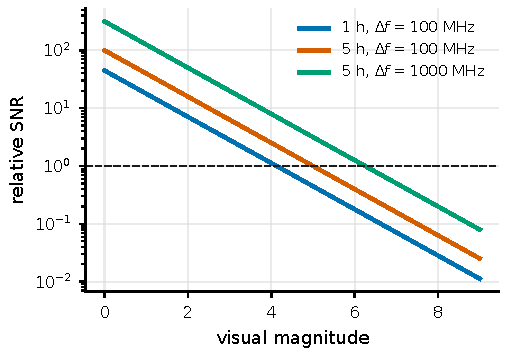
\includegraphics[width=0.86\linewidth]{figures/generated/chapter_05/ch05_snr_scaling.pdf}
\caption{The relative scaling of the intensity-interferometry SNR. For each magnitude a star is fainter, the photon spectral flux drops to about \(0.398\) of its original, and the SNR falls linearly in proportion; whereas integration time and electronic bandwidth improve the SNR only as the square root: quadruple the exposure for double the SNR. The curves omit collecting area, efficiency, background dilution, and \(|V|^2\), precisely to highlight: bright-star selection and high-speed electronics (linear factors) are far more worthwhile than "toughing out a few more nights" (the square-root factor).}
\label{fig:e11-snr-scaling}
\end{figure}

\paragraph{Substituting Real Numbers: the Order of Magnitude of Le Bohec--Holder}
\label{sec:e11-snr-lebohec}

An abstract formula must be brought down to earth by substituting real parameters. Le~Bohec and Holder, in assessing the feasibility of using Cherenkov arrays for intensity interferometry, made a classic estimate \citep{2006ApJ...649..399L}: taking two \(A=100\,{\rm m^2}\) telescopes, detection efficiency \(\alpha=0.3\), electronic bandwidth \(\Delta f=1\,{\rm GHz}\), and integration time \(T=5\,{\rm hr}\), at a baseline where the squared visibility \(|\gamma_{12}|^2=0.5\), one can measure a star of about \(V=6.7\) magnitude at \(5\sigma\) significance; for a brighter \(V=5\) magnitude star, the angular-diameter precision can reach a few percent. Compare this with the two conclusions of the last section: this \(V=6.7\) limiting sensitivity is held up almost entirely by those few linear factors (large area, high efficiency, GHz bandwidth); to push a magnitude fainter, one relies not on adding time (the square root, too expensive) but on continuing to add area and efficiency.

Set it against historical instruments, and the order of magnitude comes alive at once. Narrabri used two \(6.5\,{\rm m}\)-diameter light collectors, a \(443\,{\rm nm}\) central wavelength, a \(10\,{\rm nm}\) filter, a photocathode quantum efficiency of about 25\%, and an effective electronic bandwidth of only about \(60\,{\rm MHz}\) \citep{1967MNRAS.137..375H,1974MNRAS.167..121H,1974iiia.book.....H}. Substituting these numbers into Eq.~\eqref{eq:e11-snr} makes clear why its sample could be limited only to the very brightest stars (apparent magnitude roughly \(B<2.5\)): with area smaller than modern and bandwidth more than an order of magnitude smaller, several linear and square-root factors stacked together pin the sensitivity firmly on bright stars. VERITAS, meanwhile, uses four \(12\,{\rm m}\) telescopes, 250 MS/s sampling plus offline correlation, and can measure stellar diameters within a few hours even during the near-full-moon "dead time" unusable for gamma-ray observation \citep{2020NatAs...4.1164A}: this is exactly the result of those few linear factors (area \(\times3.4\), improved efficiency) joining forces with a wider electronic bandwidth.

\section{How to Judge Whether an Observation Is Real Signal or the Instrument Playing Tricks}
\label{sec:e11-feasibility}

The SNR formula tells you "bright enough, long enough," but it assumes the noise is clean white noise. In real observations the deadliest enemy is not white noise, but two kinds of things that masquerade as signal: \emph{background light} and \emph{systematic correlation}. Because the true signal itself is only one part in a million to one part in a thousand, any unmasked systematic effect can lead the angular-diameter fit into a ditch.

\paragraph{Background Harms in Two Ways at Once}
\label{sec:e11-background}

Moonlight, night-sky background, neighboring starlight mixed into a broadened point-spread function (PSF), detector dark current: these non-target photons are collectively called background. They harm the observation in \emph{two ways, acting simultaneously}:

\textbf{First, increasing shot noise.} Background photons must also be detected and must also take part in the coincidence count, and the shot noise they contribute directly raises the noise floor in the denominator of Eq.~\eqref{eq:e11-snr}, dragging the SNR down.

\textbf{Second, multiplying by an \(f_1f_2\) dilution factor.} Look back at Eq.~\eqref{eq:e11-correlation-model}: the correlation peak is multiplied by \(f_1f_2\), the product of the fractions of target photons out of the total photons in the two telescopes. This one is more insidious, because it is \emph{multiplicative}. Take a number: if target photons make up only 70\% in each telescope (\(f_1=f_2=0.7\)), the correlation amplitude is suppressed to
\[
  f_1 f_2 = 0.7\times0.7 = 0.49,
\]
leaving less than half. To recover the same significance from this half-strength signal, by the square-root scaling of the SNR, the integration time must be increased to about 4 times, and the longer the integration, the more likely various slow systematic drifts are to surface. Le~Bohec and Holder pointed out long ago that a Cherenkov telescope's wide optical PSF, of order \(0.05^\circ\), makes the night sky the boundary on faint-star sensitivity; modern VERITAS analysis too must specifically correct for night-sky background and dark current, or the angular diameter can be pulled off by about 10\% \citep{2006ApJ...649..399L,2020NatAs...4.1164A,2025ApJ...995..191A}. This is why narrowband filters and small-field stops are so important in intensity interferometry: they do not boost the signal, but they are the key to pushing \(f_1,f_2\) up toward 1.

\begin{figure}[tbp]
\centering
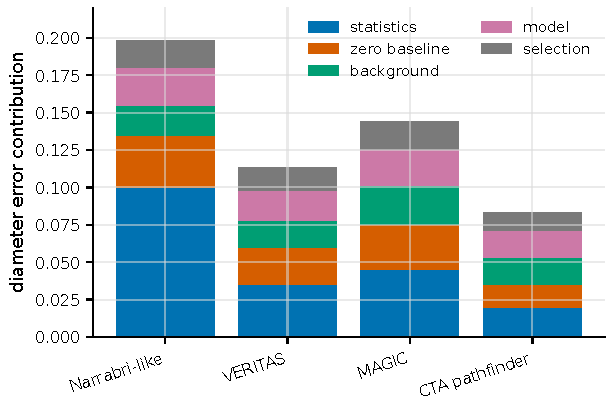
\includegraphics[width=0.82\linewidth]{figures/generated/chapter_05/ch05_error_budget.pdf}
\caption{The composition of the angular-diameter error budget in intensity interferometry. Statistical error (photon noise) falls as the square root of photon number and integration time, but zero-baseline calibration, background dilution, the stellar-atmosphere model, and weather/selection functions together build a floor of systematic error. Whether modern arrays can produce scientific results depends on whether these systematic terms, together with photon noise, can be honestly written into the likelihood function, rather than "toughed out" by the square root of time.}
\label{fig:e11-error-budget}
\end{figure}

\paragraph{Systematic Correlation Is More Dangerous Than White Noise}
\label{sec:e11-systematics}

White noise is at least "fair": it is random and can be pressed down by averaging. What truly keeps one awake is \textbf{systematic correlation}: some \emph{non-celestial}, yet synchronous, thing in the two signals. Ground reflection, a shared clock, power-supply ripple, temperature coupling, fiber crosstalk: all can inject a false correlation peak into the two electrical signals. It is more dangerous than white noise precisely because the true signal is only \(10^{-6}\) to \(10^{-3}\): however large the white noise, it tends to zero after averaging; but a systematic correlation of even \(10^{-5}\) will not be averaged away: it will sit there steadily, masquerading as a "visibility."

There is no single trick against it, only a whole set of cross-checks. The following are standard maneuvers in intensity-interferometry analysis, worth memorizing as a checklist:

\begin{itemize}
  \item \textbf{It must be zero far from zero delay.} The true thermal-light bunching peak appears only where the two signals are \emph{time-aligned}; pull the relative delay far from zero, and the correlation should return to zero. If there is a residual there, systematic correlation is at work.
  \item \textbf{The peak should vanish after swapping channels or an artificial time shift.} Swap the two signals, or deliberately insert an unphysical time offset, and the true signal peak will move or vanish with it; if the peak does not budge, it did not come from the sky.
  \item \textbf{The zero-baseline response \(N_0\) must be consistent everywhere.} Measure the same "zero-baseline" bunching height with different telescope pairs, different nights, different moon distances, and different electronic chains, and the \(N_0\) obtained should agree with one another. Once \(N_0\) shifts systematically, the \(|V|^2\) of all baselines in Eq.~\eqref{eq:e11-correlation-model} is stretched as a whole, and angular diameter, limb darkening, and oblateness all go wrong with it.
  \item \textbf{\(|V|^2\) should vary with \emph{baseline}, not with current.} The visibility of the same target should be a function only of the projected baseline \(B\); if instead it drifts along with the PMT anode current, ambient temperature, or electronic gain, then what drifts is the instrument, not the star.
\end{itemize}

MAGIC's intensity-interferometry system (MAGIC-SII) is a good example of engineering this discipline: it reuses the regular camera pixels, adds narrowband filters, transmits the signal out via VCSEL analog fiber, aggregates an electronic bandwidth of about \(110\,{\rm MHz}\), and uses a GPU real-time deadtime-free correlator to correlate online, ultimately reporting the diameters of 22 stars \citep{2024MNRAS.529.4387A}. It has pushed the limitation from "telescope area" toward "engineering stability and the calibration system," confirming exactly this: when the signal is as shallow as one part in a million, whether the systematic correlation can be held down often decides success or failure more than how large the mirror is.

\begin{figure}[tbp]
\centering
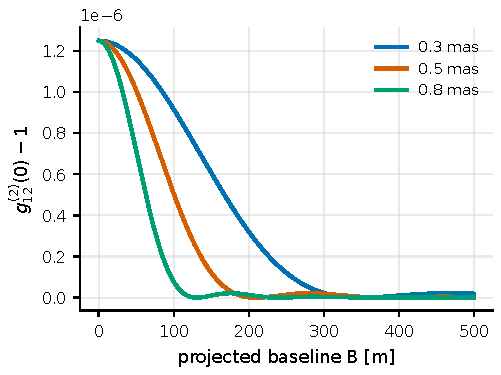
\includegraphics[width=0.86\linewidth]{figures/generated/chapter_05/ch05_sii_signal_vs_baseline.pdf}
\caption{The intensity-interferometry signal versus baseline, estimated with \(C_{12}=N_0|V|^2\) (\(N_0\) taken as \(1.25\times10^{-6}\), of the order of a modern blue-light system). The larger the star's angular diameter, the sooner \(|V|^2\) drops with baseline and shows a zero; hence the same set of baselines is more sensitive to a 0.8 mas star than to a 0.3 mas star. The first thing in observation design is to place the baselines, following the target's curve, in the "descending region," where there is both appreciable signal and maximal sensitivity to angular diameter.}
\label{fig:e11-sii-signal}
\end{figure}

\section{From Two to a Field: Multiple Baselines and uv Coverage}
\label{sec:e11-uv}

Two telescopes, however long they tough it out, can give you only a single \(|V|^2\) on \emph{one} projected baseline. And the previous chapter's van~Cittert--Zernike theorem tells us that the object's image is the inverse Fourier transform of its visibility over the whole \((u,v)\) plane. So to move from "a number" to "a picture," the only way out is to \emph{sample more spatial frequencies}. This section discusses how three things together spread the sampling from one point into a whole field.

\paragraph{More Telescopes, and the Baseline Count Explodes}
\label{sec:e11-baseline-count}

The first thing is the simplest: put out more telescopes. If the array has \(N\) telescopes, any two form a baseline, and the number of baselines that can be formed simultaneously is the combination "choose 2 from \(N\)":
\begin{equation}
  N_{\rm base}=\binom{N}{2}=\frac{N(N-1)}{2}.
  \label{eq:e11-baseline-number}
\end{equation}
\begin{formulaexplain}
\(N_{\rm base}\) is the number of telescope pairs (i.e.\ baselines) that can be formed simultaneously, and \(N\) is the number of telescopes. Each pair gives one independent baseline, so the baseline count grows explosively with array size, roughly as \(N^2/2\).
\end{formulaexplain}
The origin of the combination \(\binom{N}{2}\) is standard counting: the first telescope has \(N\) choices, the second the remaining \(N-1\), but "A-B" and "B-A" are the same baseline, so divide by 2. Substitute a few numbers to see how worthwhile it is: \(N=2\) has only 1 baseline; \(N=4\) (VERITAS) suddenly has 6; \(N=17\) has 136; and a CTAO-class few dozen to over a hundred telescopes can give thousands of baselines at once. The baseline count rising as \(N^2\) is the fundamental advantage of array telescopes over a two-antenna setup.

Here we must point out a sweet spot \emph{unique} to intensity interferometry. Amplitude interferometry (amplitude interferometry) must split the same coherent light beam optically among several beam combiners, and each split loses a share of photons, so with more paths the signal thins out. Intensity interferometry does not combine beams in optics; it first detects each telescope's light into an \emph{electrical signal}, and an electrical signal can be \textbf{losslessly copied} into arbitrarily many correlators. So one telescope's signal can be correlated with every other one at once, capturing all \(N(N-1)/2\) baselines in one go, with no "splitting light" between telescopes at all. For imaging that pursues dense \((u,v)\) coverage, this is intensity interferometry's natural bargain.

\paragraph{Let the Earth Turn for You: One Baseline Sweeps Out a Track}
\label{sec:e11-earth-rotation}

The second thing costs nothing: wait for the Earth to rotate. A telescope pair's separation vector on the ground is fixed, but its component \emph{projected onto the sky plane perpendicular to the line of sight} changes continuously as the target rises and sets in the sky. Recall the previous chapter's definition: the spatial frequency is the projected baseline divided by the wavelength, \(u=B_x/\lambda,\ v=B_y/\lambda\). As the Earth turns the target from east to west, the projected baseline \((B_x,B_y)\) varies continuously, so the same fixed telescope pair, over one night, has its sampling point \emph{draw out an arc across the \((u,v)\) plane}. This "Earth-rotation synthesis" is a decades-old stock-in-trade of radio interferometry, and it applies just as well to intensity interferometry: as long as the correlation result is stored every few minutes, one sampling point is stretched into a track.

\paragraph{Multiple Nights, Multiple Hour Angles, Multiple Telescope Pairs: Piecing Out Two-Dimensional Coverage}
\label{sec:e11-2d-coverage}

The third thing is to superpose the first two repeatedly. In one night the Earth can turn through only a segment of hour angle, drawing a finite arc; but change nights, change seasons, and observe the target at various hour angles, and the arcs join segment by segment. Then superpose the tracks of \emph{every} telescope pair in the array onto the same \((u,v)\) plot: each pair draws one, plus its conjugate point symmetric about the origin (because the real brightness distribution guarantees \(V(-u,-v)=V^*(u,v)\), so the negative-frequency point is equally a constraint), and finally, from a scattering of a few points, a two-dimensional \((u,v)\) coverage is pieced out. The denser the coverage, the finer the celestial structure that can be distinguished: sparse sampling suffices only to fit a diameter, and only dense sampling can distinguish disks, ellipses, binary stars, and even surface bright spots \citep{2008AIPC..984..205L,2012MNRAS.419..172N,2013APh....43..331D}.

\begin{figure}[tbp]
\centering
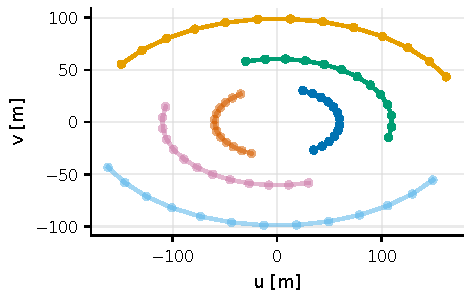
\includegraphics[width=0.82\linewidth]{figures/generated/chapter_05/ch05_uv_coverage.pdf}
\caption{A fixed telescope baseline is projected to different \((u,v)\) positions as the Earth rotates. Each colored track represents the spatial frequencies one telescope pair sweeps through over a night's hour-angle change, and the conjugate points symmetric about the origin (on the dashed side) are also effective Fourier constraints on the real brightness distribution. Superposing multiple pairs, multiple nights, and multiple hour angles grows the sampling from isolated points into two-dimensional coverage: the denser the coverage, the better one can distinguish disks, ellipses, binaries, and surface spots.}
\label{fig:e11-uv-coverage}
\end{figure}

\section{What to Do When the Phase Is Lost: Closure Phase, Phase Retrieval, and Low-Dimensional Models}
\label{sec:e11-phase}

Here we must face the innate weak spot of intensity interferometry. Amplitude interferometry directly measures the complex visibility \(V=|V|e^{i\phi}\), obtaining modulus and phase together; intensity interferometry measures only \emph{the degree of synchrony of the intensity fluctuations}, obtaining \(|V|^2\): \textbf{the phase \(\phi\) is lost}. This is no small matter: the Fourier phase encodes exactly "which way the brightness leans." The most immediate consequence of losing the phase is a kind of mirror degeneracy: a brightness distribution \(I(l,m)\) and its central-inversion mirror \(I(-l,-m)\) have \emph{exactly the same} \(|V|^2\), and the squared visibility alone can never separate the two. Measuring only the squared modulus amounts to knowing only "how much fluctuation there is" at each spatial frequency, without knowing "where the phase of the fluctuation is aligned." To reconstruct a true image, one must find a way to recover the phase information. There are three routes.

\paragraph{Route One: Third-Order Closure Phase}
\label{sec:e11-closure}

The first route inherits the third-order coherence function \(g^{(3)}\) of Chapter \ref{chap:e08}. When that third-order formula lands on three telescopes \(1,2,3\), a term appears:
\begin{equation}
  2\,{\rm Re}\big(\gamma_{12}\,\gamma_{23}\,\gamma_{31}\big),
  \label{eq:e11-triple}
\end{equation}
\begin{formulaexplain}
\(\gamma_{12},\gamma_{23},\gamma_{31}\) are the complex degrees of coherence on the three edges. Their product adds the phases of the three edges together: \(\phi_{12}+\phi_{23}+\phi_{31}\). This phase sum "once around the triangle" is the closure phase.
\end{formulaexplain}
The key lies in the phase of this triple product. Suppose each telescope introduces an unknown "piston" phase \(\psi_i\) from the atmosphere or instrument; it adds \(\psi_j-\psi_i\) to the phase of each edge. Add the three edges once around the triangle:
\[
  (\psi_2-\psi_1)+(\psi_3-\psi_2)+(\psi_1-\psi_3)=0.
\]
That annoying unknown phase of each telescope \emph{cancels exactly}! The remaining phase sum \(\phi_{12}+\phi_{23}+\phi_{31}\) belongs only to the celestial object itself, and this quantity is called the \textbf{closure phase}. It is conceptually exactly the old weapon against atmospheric jitter in amplitude interferometry, now reappearing in intensity interferometry in the guise of third-order correlation, and naturally immune to any single telescope's phase drift.

There is no free lunch: the third-order signal is much weaker than the second. The second order relies on the correlation of photons arriving \emph{in pairs}, while the third requires photons to arrive \emph{three at a time} together, and triplets are far rarer than pairs, with harsher error propagation. So the closure phase suits very large arrays and extremely bright targets, rather than being the default product of every observation.

\paragraph{Route Two: Two-Dimensional Coverage + Phase-Retrieval Algorithm + Physical Priors}
\label{sec:e11-phase-retrieval}

The second route bypasses phase measurement and \emph{solves back} the phase directly from a dense two-dimensional \(|V|\) distribution. This sounds like conjuring something from nothing, but mathematically it is not hopeless: for a real brightness distribution of compact support, its Fourier modulus and phase are not entirely independent, and the analytic structure of the modulus (via the Cauchy--Riemann relations) imposes constraints on the phase. Gerchberg--Saxton iteration \citep{1966JOSA...56..441G} and regularized reconstruction algorithms like MIRA project back and forth between the two constraints "match the measured \(|V|\)" and "satisfy the physical priors," forcing out a self-consistent phase. Here the \textbf{physical priors} are the crux: brightness non-negative, source of finite size, brightness distribution smooth, and, where necessary, a stellar-atmosphere template imposed: it is precisely these priors that filter out the mirror degeneracy and the infinitely many spurious solutions. Nuñez et al.'s simulations show that, under CTA-class \((u,v)\) coverage, bright thermal stars, fast rotators, binaries, and stars with surface spots can all be recovered to physically meaningful shape parameters, but success depends on the SNR, whether the short-baseline coverage is sufficient, and how the prior mask and image regularization are set \citep{2012MNRAS.419..172N,2012MNRAS.424.1006N,2014SPIE.9146E..0ZD}.

\paragraph{Route Three: Simply Don't Reconstruct the Image, Use a Low-Dimensional Model}
\label{sec:e11-low-dim}

The third route is the most pragmatic, and often the most powerful: \emph{do no model-free image reconstruction at all}, but take a physical model with only a few parameters and fit \(|V|^2\). Do not forget: measuring only \(|V|^2\) by no means limits one to measuring the diameter. For a large class of low-dimensional models (uniform disk, elliptical disk, binary star, limb darkening), the squared visibility can already give \emph{very strong} constraints. The visibility of a uniform disk is \(V(B)=2J_1(x)/x\) (\(x=\pi\theta B/\lambda\), with the angular diameter set in Chapter \ref{chap:e10} by the Bessel function's first zero \(x=3.8317\)); a flattened ellipse makes the zero-baseline vary with azimuth, a binary superposes a layer of cosine oscillation on \(|V|^2\), and limb darkening slightly reshapes the first lobe. All these differences can be read off from the \(|V|^2\) curve \emph{without needing the phase}. When the scientific goal is "how big is this star, how flattened, is it a binary" rather than "give me a model-independent photograph," a few-parameter model is often more stable and more credible than laborious phase retrieval.

\section{Why an Old Method Comes Back to Life: From Narrabri to CTAO}
\label{sec:e11-history}

String together all the preceding tools, and one can understand the tortuous technical history of intensity interferometry: it was once sentenced to death, and came back to life, unchanged, half a century later.

\textbf{Narrabri (1960s--1970s): proving the route works.} Australia's Narrabri Stellar Intensity Interferometer was the first instrument to fully demonstrate the scientific capability of this method. Two \(6.5\,{\rm m}\)-diameter light collectors worked on a variable rail baseline of 10--188 m, with a filter centered at about \(443\,{\rm nm}\) and bandwidth \(10\,{\rm nm}\), a photocathode quantum efficiency of about 25\%, and an effective electronic bandwidth of about \(60\,{\rm MHz}\). It measured the angular diameters of 32 stars and several binaries, the smallest diameter about \(0.4\,{\rm mas}\) \citep{1967MNRAS.137..375H,1967MNRAS.137..393H,1974MNRAS.167..121H,1974iiia.book.....H}. But it was subsequently retired, for exactly the reason that those few linear factors in Eq.~\eqref{eq:e11-snr} could not be raised at the time: movable large-area light collectors were expensive, low-noise high-speed electronics were immature, and multi-baseline imaging capability was lacking. The old method was not wrong; it was that the hardware of the time was unworthy of it.

\textbf{VERITAS (2019--): an old idea meets ready-made large mirrors.} The turning point came from atmospheric Cherenkov telescope arrays. Built originally to catch the nanosecond Cherenkov flashes triggered by gamma rays, they naturally have 10-m-class apertures, large-area mirrors, fast PMTs, long baselines, and acceptable optical image quality, exactly everything intensity interferometry had once yearned for. VERITAS uses four \(12\,{\rm m}\) telescopes to form 6 baselines at once, and measured uniform-disk diameters of \(\theta_{\rm UD}=0.523\pm0.017\,{\rm mas}\) and \(0.631\pm0.017\,{\rm mas}\) for \(\beta\)~CMa and \(\epsilon\)~Ori, at better than 5\% precision, in only a few hours, and "on the side" during near-full-moon periods unusable for gamma-ray observation \citep{2020NatAs...4.1164A}. As the \((u,v)\) coverage improved, its follow-up observations of \(\beta\)~UMa and the fast rotator \(\gamma\)~Cas advanced from "measuring a radius" to "measuring a direction-dependent shape": \(\gamma\)~Cas, using 6 baselines and over 160 pair-hours of data, yielded the oblateness of the optical photosphere, with a minor-axis diameter of about \(0.43\,{\rm mas}\), a major-to-minor axis ratio of about 1.28, and a rotation-axis position angle of about \(116^\circ\) \citep{2024ApJ...966...28A,2025ApJ...995..191A}.

\textbf{MAGIC-SII (2024): turning it into a switchable standard mode.} MAGIC uses two \(17\,{\rm m}\) parabolic telescopes, reusing the existing camera pixels, with VCSEL analog-fiber transmission and a GPU real-time deadtime-free correlator (aggregate bandwidth about \(110\,{\rm MHz}\)), achieving fast switching between regular gamma-ray observation and intensity-interferometry mode, and reported the diameters of 22 stars \citep{2024MNRAS.529.4387A}. What it demonstrates is not merely "it can measure," but "it can run stably as the routine side job of a mature facility."

\textbf{CTAO (under construction): toward kilometer baselines and thousands of baselines.} The next-generation CTAO pulls both of intensity interferometry's great levers to the full. Kilometer-scale baselines at 350--450 nm correspond to \emph{tens of microarcseconds} of resolution, one or two orders finer than Narrabri; and by Eq.~\eqref{eq:e11-baseline-number}, a few dozen to over a hundred telescopes can give \emph{thousands} of baselines and extremely dense \((u,v)\) coverage, which is exactly the prerequisite on which the phase retrieval and image reconstruction of Section \ref{sec:e11-phase} rely. It will not replace amplitude interferometers like CHARA and VLTI (which have their own strengths in sensitivity, phase capability, and the infrared band) but will become a complementary sharp tool: specializing in blue light, ultra-long baselines, bright hot stars, and fast-varying objects \citep{2013APh....43..331D,2014SPIE.9146E..0ZD}.

To close this history in one sentence: the old method came back to life not because the idea changed, but because those few linear factors in Eq.~\eqref{eq:e11-snr} (area, efficiency, bandwidth, baseline count) were finally fed to satiety all at once by Cherenkov arrays. The physics had always been there waiting; it was the hardware that arrived late.

\section{Chapter Summary}
\label{sec:e11-summary}

\begin{itemize}
  \item \textbf{The SNR formula is the first abacus.} \((S/N)_{\rm rms}=A\,\alpha\,n\,|\gamma_{12}|^2(\Delta f\,T/2)^{1/2}\): that square root comes from "averaging over \(M\sim\Delta f\,T\) independent samples, the noise shrinking as \(1/\sqrt{M}\)" (Chapter \ref{chap:e03}).
  \item \textbf{Two conclusions to memorize.} The SNR is \emph{linearly} proportional to photon spectral flux, area, and efficiency (bright stars, large mirrors are key); but grows only as \((\Delta f\,T)^{1/2}\) (quadruple the exposure for double the SNR). Improvement relies on the linear factors, not on toughing out a few more nights.
  \item \textbf{Background harms two ways.} It both increases shot noise and multiplies the correlation amplitude by \(f_1f_2\) (a 70\% target fraction leaves only 0.49). Narrowband filters and small-field stops are the key to pushing \(f_1,f_2\) up toward 1.
  \item \textbf{Systematic correlation is more dangerous than white noise,} because the true signal is only \(10^{-6}\)--\(10^{-3}\). Standard checks: the correlation should be zero far from zero delay; the peak should vanish after swapping channels/an artificial time shift; \(N_0\) must be consistent everywhere; \(|V|^2\) should vary with baseline, not with current.
  \item \textbf{Multiple baselines lead to imaging.} \(N\) telescopes give \(N(N-1)/2\) baselines; Earth rotation lets each pair's baseline sweep out a \((u,v)\) track; multiple nights and hour angles piece out two-dimensional coverage. Intensity interferometry's unique bargain: the electrical signal can be losslessly copied to many correlators, with no need to split light between telescopes.
  \item \textbf{The phase problem has three routes.} Third-order closure phase (inheriting \(g^{(3)}\) of Chapter \ref{chap:e08}, piston cancels automatically, but the signal is weak); two-dimensional coverage + phase-retrieval algorithm + physical priors; and the most pragmatic, using low-dimensional models like uniform disk / elliptical disk / binary / limb darkening, \(|V|^2\) already strongly constraining the shape.
  \item \textbf{The quantitative reason the old method revived:} Narrabri (\(6.5\,{\rm m}\), 443~nm, \(\sim60\,{\rm MHz}\), 32 stars measured, smallest \(\sim0.4\,{\rm mas}\)) \(\to\) VERITAS (\(4\times12\,{\rm m}\), \(\beta\)~CMa/\(\epsilon\)~Ori precision <5\%) \(\to\) MAGIC-SII (\(2\times17\,{\rm m}\), GPU correlator, 22 stars) \(\to\) CTAO (kilometer baselines, tens of microarcseconds, thousands of baselines). The physics did not change; the hardware fed the linear factors of Eq.~\eqref{eq:e11-snr} to satiety.
\end{itemize}

\medskip
\noindent\textbf{Questions to Ponder.}
\begin{enumerate}
  \item One star is 2.5 magnitudes fainter than another, all else equal; to measure the same SNR, by roughly how many times must the integration time be lengthened? (Hint: first use the linear factor to find how many times the SNR drops, then convert to time via the square-root scaling.)
  \item How many baselines can an array of 6 telescopes form simultaneously? If 4 more are added to make 10, how many times the original is the baseline count? What does this mean for the \((u,v)\) coverage?
  \item Why can intensity interferometry tolerate very poor optical image quality, yet is extremely sensitive to the electronic time alignment? Contrast it with "amplitude interferometry requiring the optical path stable to a small fraction of a wavelength," and say where each of the two "precision budgets" is spent.
\end{enumerate}

\chapter{Quantum Estimation, the Rayleigh Limit, and SPADE Sub-Rayleigh Resolution}
\label{chap:e12}

\begin{chapteropening}
For more than a century, when astronomers judged whether "two stars can be separated," they relied on the same sentence: the main peaks of the two diffraction spots must be far enough apart that a dip can be seen between them. This is the Rayleigh criterion. But stop and think: if I already \emph{know} that there are two equally bright stars up there, and I simply do not know how far apart they are, then does "no visible dip" really mean "the separation cannot be measured"? This chapter overhauls the whole notion of "resolution": we no longer ask "can the image plane be split into two peaks," but rather "given this many photons and this particular point spread function, how precisely can I estimate the angular separation of the two stars?" In other words, we upgrade the imaging criterion into an \textbf{estimation problem}. Once the question is posed this way, a startling fact emerges: when the two stars sit very close together, ordinary imaging throws away the separation information at a rate $\propto s^2$ (this is the so-called Rayleigh curse), yet that information \emph{never actually leaves the light field}; it is simply missed by the clumsy method of "recording position pixel by pixel." A different measurement (first projecting the light onto a set of spatial modes and then counting photons, that is, SPADE) can recover it. This chapter starts from a Gaussian point spread function and, without skipping a single step, derives all of this; finally it carries the same Fisher-information language over to kilometre-scale long-baseline intensity interferometry, to see where the weak spots of each of the two engineering routes lie.
\end{chapteropening}


\section{From "can it be split into two peaks" to "how precisely can the separation be estimated"}
\label{sec:e12-rayleigh}

Let us first sketch out the most familiar line of reasoning. A telescope of aperture $D$, working at wavelength $\lambda$, imaging a point source, produces not a point but a small diffraction spot (an Airy disk in the case of a circular aperture). For two point sources to "be separated," the classical Rayleigh criterion says: the main peak of one source's diffraction spot must fall exactly on the first dark ring of the other source's diffraction spot. For a circular aperture this angular separation is

\begin{equation}
  \theta_{\rm R}=1.22\,\frac{\lambda}{D}.
  \label{eq:e12-rayleigh}
\end{equation}
\begin{formulaexplain}
$\theta_{\rm R}$: the Rayleigh angular scale (radians). $\lambda$: the observing wavelength (metres). $D$: the telescope aperture (metres). The coefficient $1.22$ comes from the position of the first dark ring of the circular-aperture Airy disk. It is an \emph{imaging} criterion, not the ultimate limit of estimation.
\end{formulaexplain}

Let us go symbol by symbol and plug in a real number. $\theta_{\rm R}$ is in radians; to convert to the milliarcseconds customary in astronomy, multiply by $206265\times10^3$ (because $1\,\mathrm{rad}=206265''=2.06\times10^{8}\,\mathrm{mas}$). A telescope of $D=8\,\mathrm{m}$, at $\lambda=500\,\mathrm{nm}=5\times10^{-7}\,\mathrm{m}$, gives
\[
  \theta_{\rm R}=1.22\times\frac{5\times10^{-7}}{8}
  =7.6\times10^{-8}\,\mathrm{rad}
  \approx15.7\,\mathrm{mas}.
\]
For a $30\,\mathrm{m}$ giant mirror, at the same wavelength this is about $4.2\,\mathrm{mas}$. These numbers tell us how big the diffraction spot is, but they do \emph{not} tell us "whether two stars separated by only 1 milliarcsecond can actually be measured or not." To answer the latter question, we need a different language.

To make the algebra transparent, we replace the two-dimensional circular aperture with a one-dimensional Gaussian point spread function (PSF for short). This is not laziness: the Gaussian PSF preserves the core feature of "a response kernel of finite width," while letting every integral be done by hand. Write

\begin{equation}
  h(x)=\frac{1}{\sqrt{2\pi}\,\sigma}\,
       \exp\!\left(-\frac{x^{2}}{2\sigma^{2}}\right).
  \label{eq:e12-gaussian-psf}
\end{equation}
\begin{formulaexplain}
$h(x)$: the normalized point spread function (its units are the reciprocal of length or angle, and it integrates to 1). $x$: the image-plane coordinate or equivalent angular coordinate. $\sigma$: the PSF width, playing the role of the diffraction-spot radius, of order $0.4\lambda/D$ to $0.5\lambda/D$.
\end{formulaexplain}

Here, if $x$ is an angular coordinate, then $\sigma$ is the angular width $\sigma_\theta$, of order $0.5\lambda/D$: for the 8-metre mirror above, $\lambda/D=6.25\times10^{-8}\,\mathrm{rad}\approx12.9\,\mathrm{mas}$, so $\sigma_\theta\approx0.5\times12.9\approx6\,\mathrm{mas}$. It is a single number for "how fat the diffraction spot is."

Now place two \textbf{equally bright, mutually incoherent} point sources, put their centroid at the origin, one at $+s/2$ and one at $-s/2$, so the angular separation is $s$. "Mutually incoherent" is crucial: it means we must add the \emph{intensities} of the two stars separately, rather than adding the amplitudes and then squaring (this boundary was emphasized repeatedly in Chapter~\ref{chap:e10} when discussing spatial coherence). Hence the probability density for a single detected photon to land at image-plane position $x$ is the equal-weight average of two shifted PSFs:

\begin{equation}
  p(x\mid s)=\tfrac12\,h\!\left(x-\tfrac{s}{2}\right)
            +\tfrac12\,h\!\left(x+\tfrac{s}{2}\right).
  \label{eq:e12-direct-prob}
\end{equation}
\begin{formulaexplain}
$p(x\mid s)$: the probability density, given separation $s$, that one photon lands at $x$. The two $h$ terms come from the stars on either side of the centroid, and the coefficients $\tfrac12$ express equal brightness. What direct imaging sees is precisely this intensity superposition of the two diffraction spots.
\end{formulaexplain}

\paragraph{The key step: at small separations the first effect is "fattening," not "splitting"}
\label{sec:e12-taylor}

Now we carry out the first, and most counterintuitive, derivation of the chapter. We want to see: when $s\ll\sigma$, how exactly does $p(x\mid s)$ vary with $s$? The tool we use is the \textbf{Taylor expansion}, expanding a slightly shifted function in terms of its value and successive derivatives at the original point. For a shift of $\pm s/2$, expanding to second order:

\[
  h\!\left(x\pm\tfrac{s}{2}\right)
  =h(x)\;\pm\;\frac{s}{2}\,h'(x)
   \;+\;\frac{1}{2}\left(\frac{s}{2}\right)^{2}h''(x)
   \;+\;\mathcal{O}(s^{3})
  =h(x)\pm\frac{s}{2}h'(x)+\frac{s^{2}}{8}h''(x)+\mathcal{O}(s^{3}).
\]

Substitute these two into Eq.~\eqref{eq:e12-direct-prob}. Note the weight $\tfrac12$, and that \textbf{the first-order terms have opposite signs}: one star moves right, one moves left, and $\pm h'(x)$ cancel exactly. Thus

\[
  p(x\mid s)
  =\tfrac12\Big[h+\tfrac{s}{2}h'+\tfrac{s^{2}}{8}h''\Big]
  +\tfrac12\Big[h-\tfrac{s}{2}h'+\tfrac{s^{2}}{8}h''\Big]
  +\mathcal{O}(s^{4})
  =h(x)+\frac{s^{2}}{8}\,h''(x)+\mathcal{O}(s^{4}).
\]

Pause and savour this result. \emph{The separation $s$ enters the image plane at lowest order as $s^2$, and it does so through the second derivative $h''$}. The second derivative is negative at the Gaussian peak and positive in the two wings; its effect is to "press the peak down a little and lift the shoulders up a little", in other words, to make the diffraction spot \textbf{fatter}. So the first thing two nearby stars do in the image plane is not "split into two peaks" but "broaden slightly overall." "No visible two peaks" therefore \emph{does not at all mean} "no information"; the information is hidden in a second-order small quantity, and ordinary imaging merely finds it very hard to dig out of the noise.

This leads naturally to the question of the next section: this information hidden in the second-order broadening: how much is it worth? To quantify it, we need Fisher information.


\section{Fisher information and the Cramér--Rao lower bound: how much information is really in the data}
\label{sec:e12-fisher}

Suppose that one observation ultimately leaves $N_\gamma$ source photons usable for estimation (after subtracting background, bad pixels, and selection effects). The position $x_i$ of each photon is an independent sample drawn from the distribution $p(x\mid s)$. We hold a batch of $\{x_i\}$ and want to infer $s$ backwards. Statistics provides a yardstick for this class of problem: the likelihood function. It is "if the true separation is $s$, how probable is it that I observe this batch of photons." Taking the logarithm turns products into sums:

\begin{equation}
  \ln\mathcal{L}(s)=\sum_{i=1}^{N_\gamma}\ln p(x_i\mid s).
  \label{eq:e12-loglike}
\end{equation}
\begin{formulaexplain}
$\ln\mathcal{L}(s)$: the log-likelihood. $x_i$: the position of the $i$-th photon. $N_\gamma$: the effective number of source photons. It accumulates each photon's support for the hypothesis "the separation equals $s$."
\end{formulaexplain}

The sharper the likelihood is as a function of $s$, the more tightly it pins down $s$. "How sharp" is quantified by the \textbf{Fisher information}; it is the expectation of the square of the slope of the log-likelihood with respect to the parameter, and can equivalently be written as the sensitivity of the probability density to the parameter. For the single parameter $s$, with $N_\gamma$ photons independent and identically distributed,

\begin{equation}
  F_{ss}=N_\gamma\int
  \frac{1}{p(x\mid s)}
  \left[\frac{\partial p(x\mid s)}{\partial s}\right]^{2}\mathrm{d}x.
  \label{eq:e12-fisher-def}
\end{equation}
\begin{formulaexplain}
$F_{ss}$: the total Fisher information for the separation $s$ (units: angle to the power $-2$). $\partial p/\partial s$: how fast the probability density changes when the separation changes a little. $1/p$: assigns each position a statistical weight according to its probability of occurring. $N_\gamma$: the more photons, the more information.
\end{formulaexplain}

Fisher information matters because it sets a floor on the error of any \emph{unbiased} estimator $\hat s$ (unbiased: on average it is not systematically too high or too low), called the \textbf{Cramér--Rao bound}:

\begin{equation}
  \mathrm{Var}(\hat s)\ \ge\ \frac{1}{F_{ss}}.
  \label{eq:e12-crb}
\end{equation}
\begin{formulaexplain}
$\mathrm{Var}(\hat s)$: the variance of the estimator $\hat s$. The inequality says: the larger the Fisher information, the smaller the minimum statistical error any unbiased estimator can attain. Taking the square root gives $\Delta s\ge 1/\sqrt{F_{ss}}$.
\end{formulaexplain}

This inequality is the yardstick of the chapter: from now on, whenever anyone claims "I can measure a separation of 0.1 milliarcseconds," we must return to $1/\sqrt{F_{ss}}$ and check whether there is actually enough information in the data.

\paragraph{The Rayleigh curse of direct imaging: \texorpdfstring{$F_{ss}\propto s^{2}$}{Fss proportional to s squared}}
\label{sec:e12-curse}

Now substitute the expansion result of the previous section into Eq.~\eqref{eq:e12-fisher-def} to compute the Fisher information of direct imaging for the separation. We already have
\[
  p(x\mid s)=h(x)+\frac{s^{2}}{8}h''(x)+\mathcal{O}(s^{4}),
  \qquad
  \frac{\partial p}{\partial s}=\frac{s}{4}\,h''(x)+\mathcal{O}(s^{3}).
\]
(The second expression is just the term-by-term $s$-derivative of the first: $\partial_s(s^2/8)=s/4$.) Hence the integrand at small $s$ is
\[
  \frac{1}{p}\left(\frac{\partial p}{\partial s}\right)^{2}
  \approx\frac{1}{h(x)}\cdot\frac{s^{2}}{16}\big[h''(x)\big]^{2}
  =\frac{s^{2}}{16}\,\frac{[h''(x)]^{2}}{h(x)},
\]
where in the denominator $p\approx h$ (because the correction term is a higher-order small quantity of order $s^2$). What remains is to compute one integral $\int [h'']^2/h\,\mathrm{d}x$. This step uses \textbf{Gaussian moments}: for the Gaussian distribution $h$ with variance $\sigma^2$, we have $\langle x^2\rangle=\sigma^2$ and $\langle x^4\rangle=3\sigma^4$ (the three is the standard Gaussian fourth-moment factor). First compute $h''$. From Eq.~\eqref{eq:e12-gaussian-psf},
\[
  h'(x)=-\frac{x}{\sigma^{2}}h(x),\qquad
  h''(x)=\frac{x^{2}-\sigma^{2}}{\sigma^{4}}\,h(x).
\]
(The second expression: differentiate $h'=-(x/\sigma^2)h$ again, using the product rule $h''=-\tfrac1{\sigma^2}h-\tfrac{x}{\sigma^2}h'=-\tfrac1{\sigma^2}h+\tfrac{x^2}{\sigma^4}h$.) Substitute into the integral:
\[
  \int\frac{[h'']^{2}}{h}\,\mathrm{d}x
  =\int\frac{(x^{2}-\sigma^{2})^{2}}{\sigma^{8}}\,h(x)\,\mathrm{d}x
  =\frac{1}{\sigma^{8}}\big\langle(x^{2}-\sigma^{2})^{2}\big\rangle.
\]
Expand the bracket and use the two known moments:
\[
  \big\langle(x^{2}-\sigma^{2})^{2}\big\rangle
  =\langle x^{4}\rangle-2\sigma^{2}\langle x^{2}\rangle+\sigma^{4}
  =3\sigma^{4}-2\sigma^{4}+\sigma^{4}=2\sigma^{4}.
\]
So $\int[h'']^2/h\,\mathrm{d}x=2\sigma^4/\sigma^8=2/\sigma^4$. Putting it together, the Fisher information per photon is $\tfrac{s^2}{16}\cdot\tfrac{2}{\sigma^4}=\tfrac{s^2}{8\sigma^4}$, and multiplying by $N_\gamma$:

\begin{equation}
  F_{ss}^{\rm direct}\simeq N_\gamma\,\frac{s^{2}}{8\sigma^{4}},
  \qquad s\ll\sigma.
  \label{eq:e12-direct-fisher}
\end{equation}
\begin{formulaexplain}
$F_{ss}^{\rm direct}$: the Fisher information of direct imaging for the separation. The killer is that it is \emph{proportional to $s^{2}$}: the closer the two stars, the less sensitive the pixel data are to the separation, and the information drops toward zero at a quadratic rate.
\end{formulaexplain}

This is the \textbf{Rayleigh curse}: substitute Eq.~\eqref{eq:e12-direct-fisher} into the Cramér--Rao bound~\eqref{eq:e12-crb}, and the error floor $\Delta s\ge \sqrt{8}\,\sigma^2/(s\sqrt{N_\gamma})$ diverges as $s\to0$: the smaller the separation, the more photons required to reach the same precision, blowing up as $1/s^2$ \citep{2016PhRvX...6c1033T,2018Optic...5.1177P}. Written in dimensionless form with $q=s/\sigma$, the single-photon value is $F_{qq}^{\rm direct}\simeq q^2/8$, telling you in pure numbers that "below the resolution scale, direct imaging is almost blind." Figure~\ref{fig:e12-rayleigh} plots this quadratically declining blue curve.

\begin{figure}[tbp]
\centering
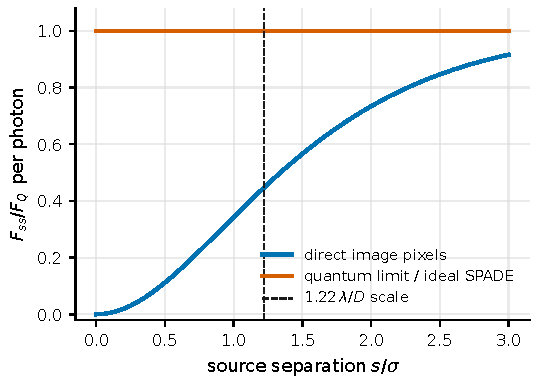
\includegraphics[width=0.82\linewidth]{figures/generated/chapter_08/ch08_rayleigh_information.pdf}
\caption{Separation information for two equally bright, incoherent Gaussian point sources. The blue curve is the direct-imaging Fisher information obtained by numerically integrating the image-plane probability density $p(x\mid s)$ (normalized to the quantum limit); at small separations it drops toward zero as $s^2$, which is the Rayleigh curse. The orange curve is the quantum limit of the next section, which remains finite even as $s\to0$. The vertical dashed line marks the commonly used Rayleigh angular scale.}
\label{fig:e12-rayleigh}
\end{figure}

\paragraph{Detection is not the same problem as estimation}
\label{sec:e12-detection}

Here we must draw a boundary that is easily overlooked. The whole Fisher-information apparatus above assumes by default that we have \emph{already accepted} the model "there are two equally bright stars up there," and simply do not know $s$. This is the estimation problem. Another class of problem is "is this really one star or two stars", this is called the \textbf{detection / model selection} problem. The two must not be conflated: in the detection problem the model dimension can change, and $s=0$ falls exactly on the \emph{boundary} of the parameter space, where the usual likelihood-ratio approximation (which assumes the parameter is at an interior point and the errors are near-Gaussian) need not hold; one must rely on simulation calibration or Bayesian evidence to decide. All the "sub-Rayleigh gains" discussed later in this chapter are, under the premise of an \emph{already accepted two-source model}, about reading the separation information already present in the light more cleanly, not about magically conjuring up a source out of nothing.

\paragraph{Multiple parameters: centroid, brightness ratio, and PSF width all compete for information}
\label{sec:e12-matrix}

In a real observation, the separation $s$ is never the only unknown. The centroid position $x_0$, the brightness ratio $r$ of the two stars, the PSF width $\sigma$, the background $b$\dots\ all must be estimated simultaneously. Then the scalar lower bound is upgraded to a \textbf{matrix} version. Arranging all parameters into a vector $\bm\theta=(s,x_0,r,\sigma,b,\dots)$, the Fisher information becomes a matrix:

\begin{equation}
  \mathrm{Cov}(\hat{\bm\theta})\ \succeq\ F^{-1},
  \qquad
  F_{\alpha\beta}=N_\gamma\int
  \frac{1}{p(x\mid\bm\theta)}
  \frac{\partial p}{\partial\theta_\alpha}
  \frac{\partial p}{\partial\theta_\beta}\,\mathrm{d}x.
  \label{eq:e12-fisher-matrix}
\end{equation}
\begin{formulaexplain}
$F_{\alpha\beta}$: the $(\alpha,\beta)$ element of the Fisher matrix, comparing the influence of parameters $\theta_\alpha$ and $\theta_\beta$ on the same data distribution. $\mathrm{Cov}(\hat{\bm\theta})\succeq F^{-1}$: the covariance matrix is no smaller than the inverse of the Fisher matrix (a matrix inequality). It is the diagonal elements of the inverse matrix that give the actual variances of the parameters.
\end{formulaexplain}

The crux is in \emph{taking the inverse}. The off-diagonal elements of $F$ record the \textbf{degeneracies} between parameters: if two parameters "look alike" in their effect on the data, their information becomes entangled, and after inversion the error is amplified. Concretely for sub-Rayleigh imaging: an unknown centroid mixes with the separation (shifting the whole image a little looks much like offsetting the two stars a little); an unknown brightness ratio redistributes information between the odd and even modes; an unknown PSF width is the most insidious: it and the binary separation both manifest as "the diffraction spot getting fatter" (recall the $s^2 h''$ term!), so the two are nearly collinear, and if $\sigma$ has not been independently calibrated tight, the binary signal will be absorbed as PSF broadening. So in reality, when reporting an error one cannot just throw out a single $1/\sqrt{F_{ss}}$; one must give the full covariance, plus the PSF calibration error, background error, and model error.


\section{Quantum Fisher information: putting the "measurement scheme" itself into the optimization}
\label{sec:e12-qfi}

At this point a sharp question surfaces: when the information of direct imaging drops toward zero, is it that the \emph{light itself} does not carry enough information, or that \emph{our measurement scheme} is too clumsy? The classical Fisher information~\eqref{eq:e12-fisher-def} is "fix the measurement scheme first (count photons pixel by pixel), then ask how much information is in the data." It takes the measurement as given. But quantum mechanics allows far more than "pixel by pixel", any orthogonal projection, any interference and mode decomposition counts.

We therefore introduce the \textbf{quantum Fisher information} (QFI): taking the optimum over \emph{all} measurements allowed by quantum mechanics, how much parameter information can in principle be read out at most from the same beam of light. It is the supremum of all classical Fisher informations, $F_{ss}\le F_{ss}^{Q}$. The QFI depends only on how the quantum state of the light field varies with the parameter, and not on which detector you choose.

To write down the state of this light, we borrow the weak-thermal-light conclusion of Chapter~\ref{chap:e06}. Celestial thermal light has a mean photon number $\epsilon\ll1$ per coherence-time mode, so the density matrix is approximately "vacuum plus a little single photon": $\rho\approx(1-\epsilon)|0\rangle\langle0|+\epsilon\,\rho_1$. That big chunk of vacuum does not click and carries no angular information: if no photon lands, you have no way to know how far apart the two stars are. What truly carries the separation information is the small fraction of detected \emph{single-photon spatial modes}. The single-photon part of two equally bright, incoherent point sources is an equal-weight mixture of two modes:

\begin{equation}
  \rho_{1}(s)=\tfrac12\,\big|\psi_{+s/2}\big\rangle\big\langle\psi_{+s/2}\big|
             +\tfrac12\,\big|\psi_{-s/2}\big\rangle\big\langle\psi_{-s/2}\big|,
  \label{eq:e12-one-photon}
\end{equation}
\begin{formulaexplain}
$\rho_1(s)$: the spatial-mode density matrix upon detecting one photon. $|\psi_{\pm s/2}\rangle$: the amplitude modes that the light of each star forms in the image plane after passing through the telescope (whose modulus squared is just the shifted PSF). Incoherent and equally bright $=$ an equal-weight probabilistic mixture of two single-photon states.
\end{formulaexplain}

Here $|\psi_{\pm s/2}\rangle$ is the amplitude PSF; for the Gaussian case $\psi(x)\propto\exp[-x^2/(4\sigma^2)]$ (its modulus squared $|\psi|^2\propto\exp[-x^2/(2\sigma^2)]=h$, with variance exactly $\sigma^2$).

Before formally throwing out the result, let us first let the reader nail down that key number for themselves. The magnitude of the QFI is ultimately determined by \emph{how easily the amplitude mode is distinguished under a shift}, and this is set by its "momentum variance" $\Delta k^2=\int(\psi')^2\,\mathrm{d}x$, a step that can be done by hand for a Gaussian. Differentiating the normalized $\psi(x)=(2\pi\sigma^2)^{-1/4}\exp[-x^2/(4\sigma^2)]$, we get $\psi'(x)=-\dfrac{x}{2\sigma^2}\psi(x)$, so
\[
  \Delta k^2=\int\big[\psi'(x)\big]^2\,\mathrm{d}x
  =\frac{1}{4\sigma^4}\int x^2\,|\psi(x)|^2\,\mathrm{d}x
  =\frac{1}{4\sigma^4}\cdot\sigma^2
  =\frac{1}{4\sigma^2},
\]
using $\int|\psi|^2\,\mathrm{d}x=1$ and $\int x^2|\psi|^2\,\mathrm{d}x=\sigma^2$ (the same Gaussian second moment). This $1/(4\sigma^2)$ is the origin of the surprisingly beautiful number in the single-photon QFI below. Under the ideal condition that the centroid, brightness, and PSF width are all known, computing the QFI rigorously for the rank-2 mixed state of Eq.~\eqref{eq:e12-one-photon}, the result is exactly $\Delta k^2$ per photon:

\begin{equation}
  F_{ss}^{Q}=N_\gamma\,\frac{1}{4\sigma^{2}}.
  \label{eq:e12-qfi}
\end{equation}
\begin{formulaexplain}
$F_{ss}^{Q}$: the \emph{upper limit} on separation information attainable by all allowed measurements. $\sigma$: the image-plane width corresponding to the amplitude mode. The crucial point is that it \emph{contains no $s$}: it does not vanish as $s\to0$, showing that the separation information sits safely in the light all along, and it is direct imaging that misses it.
\end{formulaexplain}

We need to \emph{honestly} tell the reader one thing: here we have only computed the "calibration scale" $\Delta k^2$, while treating the full proof of the rank-2 mixed-state QFI as a \textbf{known result to be cited}. It was founded by Helstrom's quantum estimation theory and given an explicit value for two-source sub-Rayleigh imaging by Tsang and collaborators, which we adopt directly here \citep{1969JSP.....1..231H,2016PhRvX...6c1033T}. The mixed-state QFI must be solved via the symmetric logarithmic derivative (SLD), and the rigorous derivation exceeds the undergraduate scope, so we do not expand it here; but the reader need not treat Eq.~\eqref{eq:e12-qfi} as "falling from the sky"; \S\ref{sec:e12-spade} will \emph{explicitly} construct the SPADE ruler and, step by step, compute the classical Fisher information up to the same $N_\gamma/(4\sigma^2)$. This confirms at least from below that $F_{ss}^{Q}\ge N_\gamma/(4\sigma^2)$ is attainable: since there exists a real measurement that reaches this value, the upper limit cannot possibly be lower.

Placing Eq.~\eqref{eq:e12-qfi} and the direct-imaging Eq.~\eqref{eq:e12-direct-fisher} side by side, the contrast is glaring:
\[
  \frac{F_{ss}^{\rm direct}}{F_{ss}^{Q}}
  =\frac{N_\gamma s^2/(8\sigma^4)}{N_\gamma/(4\sigma^2)}
  =\frac{s^2}{2\sigma^2}\ \xrightarrow{\,s\to0\,}\ 0.
\]
That is, in the sub-Rayleigh regime, the fraction of information that direct imaging uses tends to zero as $s^2$: the vast majority of information is thrown away for nothing (in Figure~\ref{fig:e12-rayleigh}, the blue curve dropping while the orange curve does not is exactly this). This is not the telescope circumventing diffraction, but the verdict of "putting the measurement scheme itself into the optimization": the information is in the light; it is a matter of whether you know how to read it \citep{1969JSP.....1..231H,2016PhRvX...6c1033T,2016OExpr..24.3684N}. The next section constructs that "reading" ruler.


\section{SPADE: translating a small separation into mode counts}
\label{sec:e12-spade}

The QFI only says "there exists an optimal measurement," not which one it is. For a Gaussian PSF and equally bright two sources, that optimal (or near-optimal) measurement has a concrete name: \textbf{spatial-mode demultiplexing} (SPADE). Its idea can be stated in one sentence: \emph{do not rush to ask which pixel the photon lands in; first ask which orthogonal spatial mode it belongs to, and then count photons in each mode separately}.

For a Gaussian PSF, the most natural set of orthogonal modes is the \textbf{Hermite--Gaussian modes}, denoted $u_0,u_1,u_2,\dots$. They are in fact old friends: the harmonic-oscillator eigenfunctions of Chapter~\ref{chap:e04}, a Gaussian times a Hermite polynomial, with $u_0$ a pure Gaussian, $u_1$ having one node, and $u_n$ having $n$ nodes. The fundamental mode $u_0$ can be taken to be exactly the amplitude PSF itself, $\psi(x)$.

\paragraph{Why the mode probabilities follow a Poisson distribution}
\label{sec:e12-poisson}

Now compute the probability that the light of one star (located at $+s/2$) lands in each mode. Its amplitude mode $\psi_{+s/2}(x)=\psi(x-s/2)$ is the fundamental mode \emph{shifted transversely} by $d=s/2$. Here we can borrow a beautiful correspondence from Chapter~\ref{chap:e04}: in the language of the harmonic oscillator, shifting the ground-state wavefunction in position by an amount $d$ yields exactly a \textbf{coherent state} $|\alpha\rangle$, and the occupation probability of a coherent state over number states (here just the mode index $n$) is a Poisson distribution $|\langle n|\alpha\rangle|^2=e^{-|\alpha|^2}|\alpha|^{2n}/n!$. The conversion between the displacement $d$ and $\alpha$ is $\alpha=d/(2x_{\rm zpf})$, and for our mode the zero-point fluctuation scale is $x_{\rm zpf}=\sigma$. So

\[
  |\alpha|^{2}=\frac{d^{2}}{4\sigma^{2}}
  =\frac{(s/2)^{2}}{4\sigma^{2}}
  =\frac{s^{2}}{16\sigma^{2}}\ \equiv\ Q.
\]

The other star at $-s/2$ has displacement $-d$, corresponding to $\alpha\to-\alpha$; but the Poisson probability depends only on $|\alpha|^2$, so positive and negative displacements give \emph{identical} mode probabilities. Hence for the equal-weight mixture of the two stars, the single-photon click probability in the $n$-th mode is

\begin{equation}
  p_{n}=e^{-Q}\,\frac{Q^{n}}{n!},
  \qquad
  Q=\frac{s^{2}}{16\sigma^{2}}.
  \label{eq:e12-spade-prob}
\end{equation}
\begin{formulaexplain}
$p_n$: the probability that a photon lands in the $n$-th Hermite--Gaussian mode. $Q$: the dimensionless "signal strength" built from the separation and the width, which is just the mean photon number of that equivalent coherent state. SPADE turns the continuous separation into a count distribution over a discrete set of modes.
\end{formulaexplain}

This Poisson shape uses the standard coherent-state result (Chapter~\ref{chap:e06}); if you would rather not borrow the harmonic oscillator, you can also directly compute the overlap integrals of the two shifted Gaussians with each Hermite--Gaussian mode, obtaining exactly the same $p_n$. Expanding at small $s$: $p_0=e^{-Q}\approx1-Q$ (almost all photons still in the fundamental mode), while
\[
  p_1=e^{-Q}Q\approx Q=\frac{s^{2}}{16\sigma^{2}},
\]
a small trickle of light leaks into the first (odd) mode $u_1$. This leakage is precisely the separation signal itself.

\paragraph{The count in the first mode, and why it circumvents the curse}
\label{sec:e12-mode-fisher}

Multiplying the probability by the photon number, the expected count in the first mode is

\begin{equation}
  \langle n_1\rangle\simeq N_\gamma\,\frac{s^{2}}{16\sigma^{2}}.
  \label{eq:e12-n1}
\end{equation}
\begin{formulaexplain}
$\langle n_1\rangle$: how many photons are expected in the first mode, equal to the total photon number times the probability $p_1$ of leaking into that mode. Small as the probability is, as long as $N_\gamma$ is large enough it can accumulate into a measurable count.
\end{formulaexplain}

Plug in real numbers. Take $s=0.1\sigma$ (well within the Rayleigh scale); then
\[
  Q=\frac{(0.1)^2}{16}=\frac{0.01}{16}=6.25\times10^{-4},
  \qquad p_1\approx6.25\times10^{-4}.
\]
Six in ten thousand: this sounds negligible. But if this bright star yields $N_\gamma=10^{8}$ source photons (a bright star can accumulate these in seconds to minutes), then in the ideal case there are $\langle n_1\rangle\approx6.3\times10^{4}$ photons in the first mode, more than enough signal-to-noise. Conversely, if the flux is only $N_\gamma=10^{5}$, the expected count is only about 63, and now dark counts, crosstalk, and background rise up to become the main limitations.

Now compute the Fisher information of the mode measurement and see how it circumvents the curse. The mode counts follow a Poisson/multinomial distribution, and their Fisher information is the weighted sum of the sensitivities of the mode probabilities to $s$:

\begin{equation}
  F_{ss}^{\rm mode}
  =N_\gamma\sum_{n}\frac{1}{p_n}
  \left(\frac{\partial p_n}{\partial s}\right)^{2}.
  \label{eq:e12-mode-fisher}
\end{equation}
\begin{formulaexplain}
$F_{ss}^{\rm mode}$: the separation Fisher information carried by the mode counts, the sum running over all spatial modes. Each term is the square of "the rate of change of the probability with $s$," divided by that mode's counting noise $p_n$.
\end{formulaexplain}

At small $s$ only the $n=1$ term matters. Using $p_1\approx s^2/(16\sigma^2)$ and its derivative $\partial p_1/\partial s\approx 2s/(16\sigma^2)=s/(8\sigma^2)$, substitute into that term:
\[
  \frac{1}{p_1}\left(\frac{\partial p_1}{\partial s}\right)^{2}
  =\frac{s^{2}/(64\sigma^{4})}{s^{2}/(16\sigma^{2})}
  =\frac{16\sigma^{2}}{64\sigma^{4}}
  =\frac{1}{4\sigma^{2}}.
\]
So

\begin{equation}
  F_{ss}^{\rm mode}\ \xrightarrow{\,s\to0\,}\ N_\gamma\,\frac{1}{4\sigma^{2}}
  \;=\;F_{ss}^{Q}.
  \label{eq:e12-mode-saturates}
\end{equation}
\begin{formulaexplain}
In the small-separation limit, the first mode alone pushes the Fisher information up to the quantum upper limit~\eqref{eq:e12-qfi}. SPADE therefore \emph{saturates} the quantum Fisher information, completely circumventing the Rayleigh curse.
\end{formulaexplain}

See clearly the mechanism of this "circumvention": $p_1$ itself shrinks as $s^2$ (weak signal), and $\partial p_1/\partial s$ shrinks as $s$ (weak slope too), but in the Fisher information it is "slope squared divided by probability," and $s^2/s^2$ \emph{cancels} exactly, leaving a finite value independent of $s$. Where does direct imaging fail? It projects photons onto position eigenstates, where the separation leaves only an $s^2$ broadening of shape (\S\ref{sec:e12-curse}), and the powers of $s$ in numerator and denominator do not match up, so it drops toward zero. SPADE switches to a different set of eigenstates (modes rather than positions), which happens to make the powers match \citep{2016PhRvX...6c1033T,2017NJPh...19b3054T}. Figure~\ref{fig:e12-spade-prob} plots the growth of the mode probabilities with $s/\sigma$, and Figure~\ref{fig:e12-direct-vs-modes} sets side by side the fact that "the image planes almost overlap while the mode counts have already separated."

\begin{figure}[tbp]
\centering
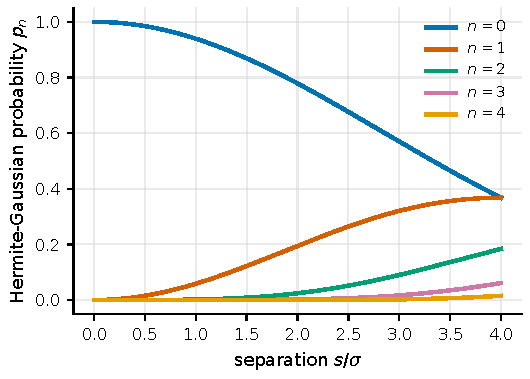
\includegraphics[width=0.82\linewidth]{figures/generated/chapter_08/ch08_spade_probabilities.pdf}
\caption{Mode probabilities for the ideal Hermite--Gaussian mode ordering. The horizontal axis is the separation $s/\sigma$, the vertical axis the single-photon probability of each mode. At small separations $p_0$ remains close to 1, while $p_1$ and the higher modes rise as powers of $Q=s^2/(16\sigma^2)$; the separation information is carried precisely by the counts of these low-probability modes.}
\label{fig:e12-spade-prob}
\end{figure}

\begin{figure}[tbp]
\centering
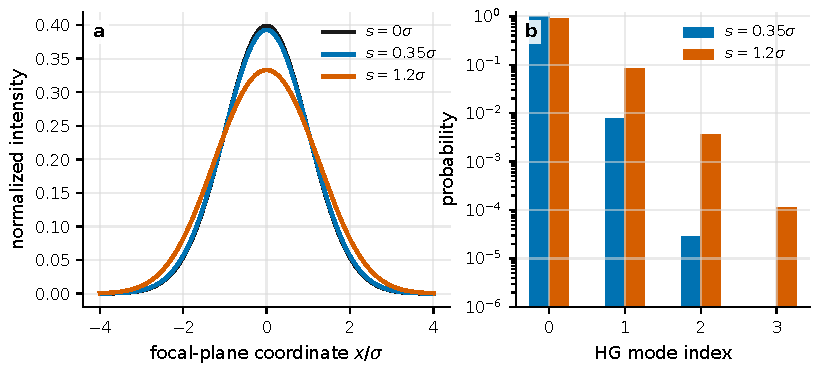
\includegraphics[width=0.92\linewidth]{figures/generated/chapter_08/ch08_direct_image_vs_modes.pdf}
\caption{The two faces of the same two-source model in the direct image and in the mode output. Left: the normalized image-plane intensity for $s=0$, $0.35\sigma$, $1.2\sigma$; in the sub-Rayleigh regime the curves differ only by an extremely weak broadening. Right: the probabilities of the first four Hermite--Gaussian modes at $s=0.35\sigma$ and $1.2\sigma$; small as the low-order non-fundamental-mode probabilities are, they turn the separation into perfectly clear mode counts.}
\label{fig:e12-direct-vs-modes}
\end{figure}


\section{Real-world limitations: the quantum bound is not automatically attainable}
\label{sec:e12-reality}

The beautiful Eq.~\eqref{eq:e12-mode-saturates} has one big premise: the mode basis is aligned exactly with the true centroid, and the mode sorter has no crosstalk and no background leakage. In reality all of these must be discounted, and the quantum bound is held up by a layer of \textbf{systematic floor}.

The most deadly is the \textbf{centroid / pointing error}. SPADE's first mode $u_1$ holds the signal through "the transverse asymmetry of the whole image relative to the mode centre." But if the whole image is shifted by $\delta x$ overall due to pointing jitter or tracking error, then this shift \emph{itself} pours light into $u_1$, and by exactly the same mechanism as the true signal. Using the same coherent-state conversion as the previous section, the fraction of an overall shift $\delta x$ leaking into the first mode is
\[
  p_1^{\rm leak}\approx\frac{\delta x^{2}}{4\sigma^{2}},
\]
while the true binary signal is $p_1^{\rm sig}\approx s^2/(16\sigma^2)$. The condition for the two to be equal is
\[
  \frac{\delta x^{2}}{4\sigma^{2}}=\frac{s^{2}}{16\sigma^{2}}
  \ \Longrightarrow\ \delta x=\frac{s}{2}.
\]
In other words, as soon as the centroid calibration error reaches half the separation, the spurious signal is of the same order as the true signal, and then the first-mode count you measure simply cannot distinguish "two stars" from "the telescope being misaligned." To measure a separation of $s=0.1\sigma$, one must stabilize and calibrate the centroid to far better than $0.05\sigma$, a very hard requirement on pointing, tracking, and calibration.

Beyond this there is a string of real-world killers: the \textbf{crosstalk} matrix of the mode sorter is unstable and leaks a little of the strong $u_0$ light into $u_1$, drowning the few-parts-in-ten-thousand signal; \textbf{background light}, if it does not have the same spatial-mode distribution as the source, lays a floor of noise across all modes; an insufficient Strehl ratio, aberrations drifting with time, dispersion, and polarization crosstalk all contaminate the mode response matrix. The common feature of these effects is that they \emph{do not decrease with $N_\gamma$}. The statistical error falls all the way down as $1/\sqrt{N_\gamma}$, but once it hits the systematic floor, adding more photons does not help (the green curve in Figure~\ref{fig:e12-crb} that flattens once calibration error is added is exactly this). So "reaching the quantum bound" is never automatic; experimentally, the more common approach is a simpler, more robust phase-sensitive measurement (a phase plate, SLIVER, SPLICE, and the like), which mitigates the quadratic loss of direct imaging, but whose actual gain is still dictated by visibility, crosstalk, and alignment error \citep{2017PhRvL.118g0801T,2019NJPh...21i3010B,2018Optic...5.1177P}.

\begin{figure}[tbp]
\centering
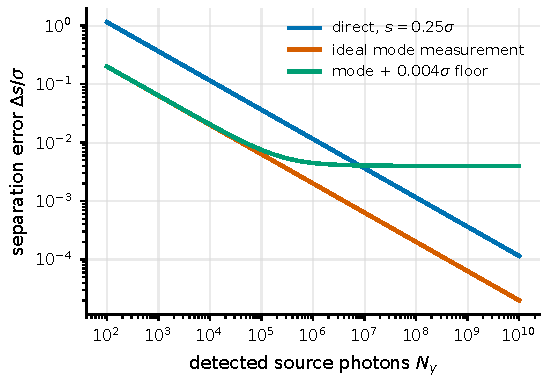
\includegraphics[width=0.82\linewidth]{figures/generated/chapter_08/ch08_cramer_rao_bound.pdf}
\caption{Cramér--Rao separation error for a sub-Rayleigh two-source system. The horizontal axis is the number of detected source photons $N_\gamma$, the vertical axis $\Delta s/\sigma$. The ideal mode measurement falls all the way down as $N_\gamma^{-1/2}$; direct imaging, with much smaller Fisher information, needs many more photons to catch up. The green curve, after adding a small piece of mode-matching systematic error, develops a plateau: continuing to add photons cannot remove the calibration error.}
\label{fig:e12-crb}
\end{figure}

There is a subtler premise still: the \textbf{partial coherence} of the source. Throughout the above we assumed the two stars are mutually incoherent (an equal-weight probabilistic mixture). Larson and Saleh pointed out that as the source becomes partially coherent, the Rayleigh curse may \emph{reappear}; Tsang and Nair subsequently clarified that as long as it is not the degenerate case of fully positive correlation, and one performs the correct Fisher computation for weak thermal light, SPADE still avoids the total vanishing of small-separation information \citep{2018Optic...5.1382L,2019Optic...6..400T}. In astronomy one must especially distinguish two things: whether two emitting regions on the source surface \emph{themselves} radiate independently, and the spatial coherence built up after the light propagates to the telescope by the van Cittert--Zernike theorem (Chapter~\ref{chap:e10}), are two different matters. The latter is precisely the quantity that interferometry measures, and cannot be simply equated with the coherence of the source's own emission.


\section{The long-baseline version: intensity interferometry does the same thing in the Fourier plane}
\label{sec:e12-sii}

The previous sections dealt with spatial-mode measurement at a single aperture, or after coherent beam combination. But this whole idea of "treating resolution as an estimation problem" can be carried over entirely to kilometre-scale long-baseline arrays, only this time the stage shifts from the image plane to the \textbf{Fourier plane}. Chapters~\ref{chap:e10} and~\ref{chap:e11} explained: the baseline between different pairs of telescopes samples different spatial frequencies of the sky brightness distribution; the constraint on the data comes from \emph{how the visibility varies with baseline}. Here "sub-Rayleigh" is no longer about reading two peaks out of one diffraction spot, but about measuring the Fourier modulus of the source brightness distribution on a long baseline.

Intensity interferometry does not measure the first-order field phase but the correlation of the intensity \emph{fluctuations} of two telescopes. Under ideal thermal light, the second-order correlation at zero delay (the Siegert/HBT relation of Chapter~\ref{chap:e10}) gives

\begin{equation}
  g_{ij}^{(2)}(0)-1=\big|\gamma_{ij}\big|^{2},
  \label{eq:e12-hbt}
\end{equation}
\begin{formulaexplain}
$g_{ij}^{(2)}(0)$: the zero-delay second-order correlation of telescopes $i,j$; subtracting 1 gives the excess relative to a "completely uncorrelated" baseline. $\gamma_{ij}$: the normalized complex degree of coherence, equal to the first-order visibility $V$. The degree of synchrony of the intensity fluctuations directly gives the squared visibility amplitude.
\end{formulaexplain}

The observable is therefore a series of squared visibilities across baselines/spectral channels/time intervals:

\begin{equation}
  d_{k}=\big|V(u_k,v_k;\bm\theta)\big|^{2}+\eta_{k},
  \label{eq:e12-sii-data}
\end{equation}
\begin{formulaexplain}
$d_k$: the squared visibility measured on the $k$-th baseline/time/spectral channel. $V$: the model visibility determined by the source parameters $\bm\theta$. $\eta_k$: the noise. The angular structure is written into how $|V|^2$ varies with baseline.
\end{formulaexplain}

Apply the same Cramér--Rao logic. For a parameter $\theta_\alpha$, the Fisher matrix of intensity interferometry is

\begin{equation}
  F_{\alpha\beta}^{\rm SII}
  =\sum_{k,l}
  \frac{\partial|V_k|^{2}}{\partial\theta_\alpha}\,
  C^{-1}_{kl}\,
  \frac{\partial|V_l|^{2}}{\partial\theta_\beta},
  \label{eq:e12-sii-fisher}
\end{equation}
\begin{formulaexplain}
$F_{\alpha\beta}^{\rm SII}$: the Fisher matrix of the intensity-interferometry data. $C^{-1}_{kl}$: the inverse of the measurement-error covariance of $|V|^2$, weighting the data points. The steeper the dependence of the squared visibility on a parameter, and the smaller its error, the more information.
\end{formulaexplain}

Here $C_{kl}$ is the covariance of the measurement error of $|V|^2$, which can be estimated using time-shifted background, empty baselines, overnight repeat observations, or injected simulations. If the errors of the data points are approximately independent, $C$ becomes diagonal, and Eq.~\eqref{eq:e12-sii-fisher} reduces to "the sum of each point's slope squared divided by variance", the same thing as the single-parameter Eq.~\eqref{eq:e12-fisher-def}, only with a sum replacing the integral. The crux is that \emph{slope} $\partial|V|^2/\partial\theta$: it tells you which baseline is most useful.

Plug in a concrete model: a uniform-disk star. Its visibility is a first-order Bessel function (this comes from the Fourier transform of the disk brightness distribution, derived in Chapter~\ref{chap:e10}):

\begin{equation}
  V(x)=\frac{2J_1(x)}{x},
  \qquad x=\frac{\pi B\theta_\star}{\lambda},
  \label{eq:e12-uniform-disk}
\end{equation}
\begin{formulaexplain}
$V(x)$: the visibility of a uniform disk. $J_1$: the first-order Bessel function. $B$: the projected baseline (metres). $\theta_\star$: the angular diameter of the star. The baseline scans the Fourier modulus of the disk through the dimensionless $x$.
\end{formulaexplain}

$V(x)$ equals 1 at $x=0$, decreases as $x$ grows to its first zero (the first nontrivial zero of $J_1$ is at $x\approx3.83$, the standard Bessel zero), and then turns over into a series of progressively weaker sidelobes. The most useful baseline for the angular diameter $\theta_\star$ falls where the slope $\partial|V|^2/\partial\theta_\star$ of $|V|^2$ is largest, usually along the section where the visibility drops rapidly. On short baselines $V\approx1$ and barely varies with $\theta_\star$ (no slope on the plateau, no information); on extremely long baselines the signal falls into the sidelobes and is easily overwhelmed by systematic errors. So "longer baseline is not always better"; rather, one should \emph{choose where the slope is large}. Figure~\ref{fig:e12-sii-fisher} plots this design principle very plainly.

\begin{figure}[tbp]
\centering
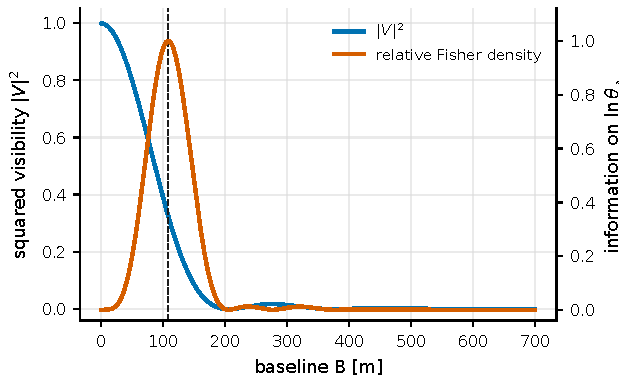
\includegraphics[width=0.82\linewidth]{figures/generated/chapter_08/ch08_visibility_fisher_design.pdf}
\caption{The relation between baseline choice and parameter information in intensity interferometry. The blue curve is the squared visibility of a uniform disk with $\lambda=450~\mathrm{nm}$ and $\theta_\star=0.55~\mathrm{mas}$; the orange curve is the Fisher weight computed from $\partial|V|^2/\partial\ln\theta_\star$ and normalized. The most useful baseline falls where the visibility drops rapidly; simply lengthening or shortening the baseline does not automatically add angular-diameter information.}
\label{fig:e12-sii-fisher}
\end{figure}

The price of intensity interferometry is \textbf{phase loss}: $|V|^2$ discards the phase of $V$, and is therefore insensitive to overall translation and brings mirror and central-symmetry degeneracies: the orientation of a binary, the position of a bright spot, or an asymmetric disk often must be mitigated by the $uv$ coverage from Earth's rotation, multiple wavelengths, prior models, or third-order correlations. What it buys in return is enormous: near-immunity to atmospheric phase disturbances. Because it only compares whether the \emph{intensity} fluctuations of the two paths are synchronous, the telescopes need only an electronic connection and to align their signals in time to a small fraction of the detector response, without maintaining optical coherence (Chapter~\ref{chap:e10} showed that nanosecond-level electronic timing corresponds to a path-length tolerance of tens of centimetres, and the atmospheric piston jitter of a few nanometres falls entirely within that tolerance). For exactly this reason, atmospheric Cherenkov telescope arrays (whose optical image quality is far inferior to that of professional interferometers but which enjoy large collecting area and long baselines) turn out to be ideal intensity-interferometry arrays \citep{1956Natur.177...27B,1974MNRAS.167..121H,2020NatAs...4.1164A,2024MNRAS.529.4387A}.

\paragraph{The division of labour between the two engineering routes}
\label{sec:e12-two-roads}

Placing the two kinds of "sub-Rayleigh estimation" side by side, their engineering bottlenecks are exactly opposite, and so their suitable targets differ:

\begin{itemize}
  \item \textbf{SPADE / spatial-mode measurement} (single aperture or coherent beam combination): requires a \emph{stable wavefront}. The target light must be coupled into fibre modes, an integrated-optics chip, or a free-space mode sorter, with adaptive optics squeezing the incident light into as few controllable modes as possible. Its enemies are the Strehl ratio, non-common-path aberrations, centroid jitter, and mode crosstalk. It suits few-parameter problems such as reading the angular separation of two nearby stars or the low-order shape moments of a star.
  \item \textbf{Intensity interferometry} (long-baseline arrays): simply \emph{accepts} that the atmosphere randomizes the phase, and trades large collecting area and long baselines for $|V|^2$ information. Its enemies are low photon rate, electronic bandwidth, background, time synchronization, and systematic covariance. It suits bright hot stars, rapid rotators, binaries, and angular-diameter measurements.
\end{itemize}

Whichever route one takes, a publishable sub-Rayleigh estimate must present four sets of accounts at once: the \emph{photon budget} (magnitude, spectral band, total efficiency, exposure $\to$ effective $N_\gamma$); the \emph{angular scale} ($\lambda/D$, PSF width $\sigma_\theta$, candidate separation $s$ or angular diameter $\theta_\star$); the \emph{measurement matrix} (pixel response, mode crosstalk, or the $|V|^2$ covariance); and the \emph{model boundaries and error decomposition} (how equally bright two sources, an unknown brightness ratio, a finite disk, partial coherence, or a background star rewrite the Fisher matrix). Finally, checking one criterion is enough to diagnose: is the statistical error still falling as $N_\gamma^{-1/2}$? If it is no longer falling, chances are that alignment, PSF, background, correlator, or model errors have hit a plateau. Putting these boundaries into the final inference commonly uses Bayesian sampling and evidence comparison: direct-imaging, mode-count, and intensity-interferometry data can share the same parameter vector, with joint likelihoods multiplied; priors such as a known orbit, colour, spectral type, and distance directly reshape the identifiable parameter space \citep{2009MNRAS.398.1601F,2013PASP..125..306F}.


\section{Chapter Summary}
\label{sec:e12-summary}

\begin{itemize}
  \item \textbf{Resolution is an estimation problem, not an imaging criterion.} The Rayleigh criterion $\theta_{\rm R}=1.22\lambda/D$ only asks "can the image plane be split into two peaks"; the real question to ask is "given $N_\gamma$ photons, how precisely can the separation $s$ be estimated," and the answer is given by the Fisher information and the Cramér--Rao bound $\mathrm{Var}(\hat s)\ge1/F_{ss}$.
  \item \textbf{At small separations, the first effect is fattening, not splitting.} Taylor-expanding the two shifted PSFs, the first-order terms cancel and $p(x\mid s)=h+\tfrac{s^2}{8}h''+\mathcal O(s^4)$. The separation appears at lowest order as a second-order broadening through $h''$, and the direct-imaging Fisher information $F_{ss}^{\rm direct}\simeq N_\gamma s^2/(8\sigma^4)\to0$: this is the Rayleigh curse.
  \item \textbf{The information never leaves the light.} The quantum Fisher information replaces "pixel by pixel" with "all allowed measurements," giving for the weak-thermal single-photon state $F_{ss}^{Q}=N_\gamma/(4\sigma^2)$, which does not vanish as $s\to0$. The curse is a disease of the measurement scheme, not of the light.
  \item \textbf{SPADE saturates the quantum limit.} Projecting onto Hermite--Gaussian modes and then counting, the mode probabilities follow a Poisson distribution $p_n=e^{-Q}Q^n/n!$ with $Q=s^2/(16\sigma^2)$. In the first mode $p_1\propto s^2$ and $\partial p_1/\partial s\propto s$, and their ratio in the Fisher information leaves the finite limit $N_\gamma/(4\sigma^2)$, circumventing the curse.
  \item \textbf{The bound is not automatically attainable.} The amount of a centroid error $\delta x$ leaking into the first mode is $\delta x^2/(4\sigma^2)$, which becomes of the same order as the signal $s^2/(16\sigma^2)$ when $\delta x\sim s/2$; crosstalk, background modes, and partial coherence all create a systematic floor that does not decrease with $N_\gamma$.
  \item \textbf{The long baseline is the Fourier version of the same thing.} Intensity interferometry estimates parameters in the Fourier plane, $F^{\rm SII}_{\alpha\beta}=\sum\partial|V|^2/\partial\theta\,C^{-1}\,\partial|V|^2/\partial\theta$, and the most useful baseline is where the slope of $|V|^2$ is large. It discards the phase and is immune to the atmosphere, complementing SPADE's "stable-wavefront" route.
\end{itemize}

\medskip
\noindent\textbf{Questions to Ponder.}
\begin{enumerate}
  \item If the \emph{brightness ratio} of the two stars is also set as an unknown parameter, how much separation information remains in the first (odd) mode and in the fundamental (even) mode respectively? Why does the degeneracy of an "unknown brightness ratio" weaken the contribution of the odd mode?
  \item The direct-imaging result $F_{ss}^{\rm direct}\propto s^2$ was derived under a \emph{Gaussian} PSF. If one switches to an Airy PSF with real sidelobes, does the second-order broadening step change? Is the Rayleigh curse a peculiarity of the Gaussian, or a more general phenomenon?
  \item Intensity interferometry discards the phase, while SPADE retains information on the relative phase of the modes. For the task of "measuring the \emph{orientation} of two nearby stars," which has the advantage? Translate it into the degeneracy in Eq.~\eqref{eq:e12-sii-fisher} to explain.
\end{enumerate}


% ============================================================
\part{Instruments, Event Tables, and Observation Design}
\chapter{Detectors, Clocks, and Event Tables}
\label{chap:e13}

\begin{chapteropening}
Chapter~\ref{chap:e07} told us that the essence of detection is "absorb one photon, spit out one electrical pulse"; Chapter~\ref{chap:e08} then told us that the correlation peak hidden in the event stream can be as small as $10^{-6}$, and will be convolutionally broadened and diluted by the detector's finite temporal response. Yet both of those chapters still remained at the level of an "ideal detector." Real telescopes have no ideal detector: a photon striking the photocathode has only a certain probability of turning into an electron; the arrival time of each electrical pulse carries a random jitter of tens of picoseconds to a few nanoseconds; every time the detector fires it must "catch its breath," blind to new photons during this dead time; and the clocks of two telescopes a hundred metres apart must still be aligned to the picosecond. This chapter answers a very "hardware" question: a photon, through exactly which stages does it pass before it becomes that one \emph{time-stamped record} in the event table? We will take apart quantum efficiency, timing jitter, dead time and pile-up, afterpulsing, and clock synchronization one by one, deriving every formula from beginning to end, and finally landing on the most practical checklist of all: "which fields should the event table store?"
\end{chapteropening}

\section{From a photon to one time-stamped event}
\label{sec:e13-from-photon-to-event}

Let us first catch the conclusion of the previous stage. Chapter~\ref{chap:e07} described "detection" as a probabilistic event: a photon of energy $h\nu$ strikes the detector and has a certain probability of being absorbed and triggering a recordable electrical pulse. Chapter~\ref{chap:e08} lined up these electrical pulses into a string of time-stamped "clicks," and taught us to read $g^{(2)}(\tau)$ out of them. But the detector there was "transparent": photons in, events out, with no loss, delay, or saturation in between. Real devices are exactly the opposite: they set up several checkpoints between the photon and the event, and each checkpoint rewrites the event rate, the time stamp, or the peak shape. This chapter is about opening up each of these checkpoints one by one.

The key data structure is called the \textbf{event table} (event list). It differs fundamentally from an ordinary light curve. A light curve is "accumulate the photon count of a stretch of exposure into one time bin", once accumulated, who came at what moment, from which telescope, at which wavelength, in which polarization, is all smeared into a single number. The event table is the opposite: it preserves information \emph{photon by photon}: arrival time, telescope number, detector channel, wavelength channel, polarization channel, weight, quality flag. Why is it worth being this "verbose" in storage? Because for measurements such as second-order correlation, pulsar folding, and rapid occultation, the signal is hidden precisely in the joint information of "which two photons arrived almost simultaneously"; as soon as you accumulate into time bins too early, the correlation peak you seek is erased and can never be recovered afterwards. Iqueye was designed this way: it saves every photon with a time tag, then offline selects any time bin from 24.41 ps to minute scale; a single observation of $\zeta$ Ori produced about $2\times10^{10}$ photon events, about 78 GB of data \citep{2009A&A...508..531N,2019CoSka..49...85Z}. Clearly the event table is not an optional auxiliary file but the primary data product of a real telescope.

Writing down one raw event, it looks like this:
\begin{equation}
  \mathcal{E}^{\rm raw}_q =
  \big(n_q,\ a_q,\ d_q,\ c_q,\ p_q,\ f_q,\ w_q\big),
  \qquad
  t^{\rm raw}_q=t_0+n_q\,\delta t+\epsilon_{\rm roll}.
  \label{eq:e13-raw-event}
\end{equation}
\begin{formulaexplain}
$\mathcal E_q^{\rm raw}$ is the $q$-th raw event; $n_q$ is the clock count (tick), $\delta t$ is the duration of one tick, $t_0$ is the start of the recording segment, and $\epsilon_{\rm roll}$ handles counter overflow. It translates one electronic record into the earliest event time.
\end{formulaexplain}
Let us pin down each symbol. The subscript $q$ numbers the $q$-th event. $n_q$ is the integer number of ticks read by the electronic counter (dimensionless); $\delta t$ is the time corresponding to one tick (units of seconds), and for modern time-to-digital converters (TDCs) $\delta t$ is often in the range $10^{-11}$--$10^{-10}\,{\rm s}$; commercial multi-channel TCSPC systems can reach a basic timing resolution of 80 ps, and Iqueye's quantization step is 24.41 ps \citep{2009A&A...508..531N,2020RScI...91a3108W}. $t_0$ is the start moment of the recording segment (seconds), and $\epsilon_{\rm roll}$ handles counter rollover after reaching full scale, or segmentation. The remaining integers are all "labels": $a_q$ is the telescope or station number, $d_q$ is the detector number, $c_q$ is the wavelength channel or filter number, $p_q$ is the polarization channel, $f_q$ is the quality flag, and $w_q$ is the event weight. Overflows, dropped packets, saturation, clouds, pointing anomalies, and electronics anomalies should all be written into $f_q$; otherwise, when a strange peak later appears in the correlation function, you will have no way to trace whether it is celestial or a fault.

\begin{figure}[tbp]
\centering
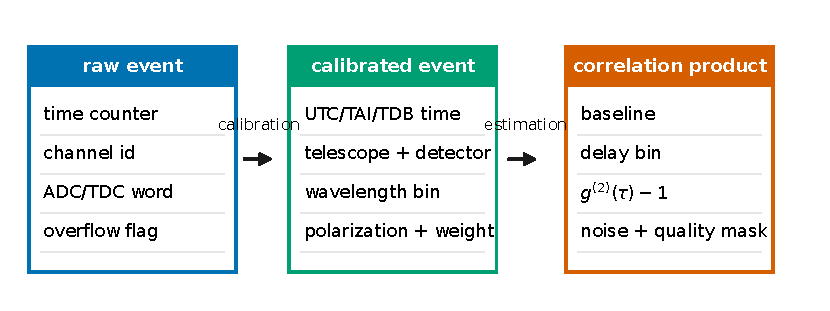
\includegraphics[width=0.96\linewidth]{figures/generated/chapter_06/ch06_event_table_schema.pdf}
\caption{Event data flow from the raw electronic record to the calibrated event table, and then to the correlation-function product. The raw layer stores counter time, channel numbers, and overflow flags; the calibrated layer converts time to a unified time scale and adds telescope, wavelength, polarization, and weight; the correlation-product layer finally records baseline, delay bin, correlation amplitude, and noise estimate. If only the light curve is stored at the first layer, the later clock, wavelength, and polarization selections can no longer be re-executed.}
\label{fig:e13-event-table-schema}
\end{figure}

The road map of this chapter is therefore clear: first look at how a photon turns into an electron event with probability $\eta$ (Section~\ref{sec:e13-detectors}), then look at how much jitter each event time carries and how it convolutionally widens the correlation peak (Section~\ref{sec:e13-jitter}), then look at how the "catching-breath" dead time and pile-up cause the recording rate to saturate (Section~\ref{sec:e13-deadtime}), how afterpulsing forges a short-delay correlation (Section~\ref{sec:e13-afterpulse}), then align the clocks of two telescopes to the picosecond (Section~\ref{sec:e13-clock}), and finally land on the event-table field checklist (Section~\ref{sec:e13-schema}) and the trade-off between spectral resolution and coherence time (Section~\ref{sec:e13-spectral}).

\section{Detectors: quantum efficiency turns photons into electron events}
\label{sec:e13-detectors}

The first and most basic role of a detector is to determine "how many incident photons really became electron events." The core parameter of this step is called the \textbf{quantum efficiency} $\eta$: the probability that a photon arriving at the photosensitive surface is absorbed and triggers one countable pulse. It is dimensionless, takes values between 0 and 1, and depends strongly on wavelength. Multiplying together the efficiencies along the entire optical path, the mean detection rate of a channel is
\begin{equation}
  R_{\rm det}
  =
  A_{\rm eff}
  \int_{\lambda_1}^{\lambda_2}
  F_\lambda(\lambda)\,
  T_{\rm opt}(\lambda)\,
  \eta(\lambda)\,
  d\lambda
  \;+\;R_{\rm sky}+R_{\rm dark}.
  \label{eq:e13-detected-rate}
\end{equation}
\begin{formulaexplain}
$R_{\rm det}$ is the detected count rate; $A_{\rm eff}$ is the effective collecting area; $F_\lambda$, $T_{\rm opt}$, $\eta$ are respectively the source photon spectral flux, the optical-path transmission, and the quantum efficiency; $R_{\rm sky},R_{\rm dark}$ are the sky background and dark counts. It is an "event-rate budget."
\end{formulaexplain}
Let us go term by term through the units and orders of magnitude. $A_{\rm eff}$ is the effective collecting area (${\rm m}^2$), which for atmospheric Cherenkov telescopes can reach tens to over a hundred ${\rm m}^2$. $F_\lambda$ is the source's photon spectral flux density (${\rm photons\,s^{-1}\,m^{-2}\,nm^{-1}}$). $T_{\rm opt}$ is the total transmission of mirrors, filters, fibres, collimators, and windows (dimensionless, usually much less than 1). $\eta(\lambda)$ is the quantum efficiency. $R_{\rm sky}$ is the count rate of skyglow and stray light, and $R_{\rm dark}$ is the dark count rate the detector produces spontaneously even in complete darkness (both in units of ${\rm s}^{-1}$). The structure of the formula is very plain: the source contribution is "area $\times$ spectral flux $\times$ transmission $\times$ efficiency" integrated over the bandwidth, plus two source-independent background terms. The signal-to-noise ratio of intensity interferometry is ultimately determined jointly by "the stellar photon rate diluted by background, and the intensity fluctuations"; MAGIC-SII directly uses the PMT DC current to estimate the photon flux and background pixels to correct for night-sky light, while VERITAS-SII uses off-source measurements to estimate the background and then corrects the correlation amplitude by the stellar-light fraction \citep{2020NatAs...4.1164A,2024MNRAS.529.4387A}.

Different tasks require different detectors, which trade off among "efficiency, timing resolution, area, dark counts." Placing the common classes side by side:

\begin{itemize}
  \item \textbf{Photomultiplier tube (PMT)}: photons strike the photocathode and knock out photoelectrons, which are multiplied stage by stage through a string of dynodes, reaching gains of order $10^6$. It has a large area, high gain, and narrow pulses (ns-scale), naturally matching the high-speed electronic chain of Cherenkov telescopes; its blue quantum efficiency is often $20\%$--$40\%$, and the PMT used by VERITAS-SII at 416 nm has a quantum efficiency of about $30\%$ \citep{2020NatAs...4.1164A,2024MNRAS.529.4387A}. It is the workhorse detector of contemporary ground-based intensity interferometry.
  \item \textbf{Avalanche photodiode (APD)}: a semiconductor device that amplifies the signal via avalanche multiplication under reverse bias. Working in \emph{linear mode} with a bias below the breakdown voltage, its output is proportional to the incident intensity, with moderate gain and relatively low noise, suited to moderate to strong light flux, but usually not used for single-photon counting.
  \item \textbf{Single-photon avalanche diode (SPAD)}: biasing the APD \emph{above the breakdown voltage} (Geiger mode), one photoelectron can trigger a self-sustaining avalanche, producing a digital "yes/no" pulse. Its visible-light quantum efficiency can reach $50\%$--$60\%$, its single-photon timing resolution is about 30--50 ps, and its dark counts are commonly 10--100 ${\rm s}^{-1}$; the price is a small photosensitive area, relatively long dead time, and afterpulsing following the avalanche that contaminates the short-delay correlation (detailed below) \citep{1996ApOpt..35.1956C,2009JMOp...56..261B,2009A&A...508..531N,2015SPIE.9504E..0CZ}.
  \item \textbf{Silicon photomultiplier (SiPM)}: hundreds to thousands of tiny SPAD cells (microcells) are connected in parallel into a planar array, each cell reporting only "yes/no," and summing their outputs gives a signal approximately proportional to the photon number. It combines single-photon sensitivity with a relatively large effective area, has low power consumption, and is not damaged by strong light; it has already entered the new generation of Cherenkov cameras. The price is optical crosstalk between cells, and a dark count rate higher than a single SPAD.
  \item \textbf{Superconducting nanowire single-photon detector (SNSPD)}: a superconducting nanowire biased near its critical current is cooled to a few kelvin, and the absorption of one photon is enough to destroy the local superconducting state, producing a recordable voltage pulse. It simultaneously achieves high quantum efficiency (up to over $90\%$), extremely low dark counts (as low as below the ${\rm s}^{-1}$ scale), and picosecond-scale timing jitter, making it the strongest single-photon detector in overall timing and dark-count performance; the price is that it requires a cryogenic cooling system and has a small photosensitive area.
  \item \textbf{Energy-resolving detectors (e.g. MKID, microwave kinetic inductance detector)}: these superconducting devices, after absorbing one photon, have their superconducting kinetic inductance vary with the incident photon energy, so they can \emph{directly read out the wavelength of each photon}, inherently carrying spectral channels. The price is that their timing resolution is usually only microsecond-scale with a long dead time, and they likewise require a cryogenic system: they trade timing resolution for energy (wavelength) resolution.
\end{itemize}

\begin{figure}[tbp]
\centering
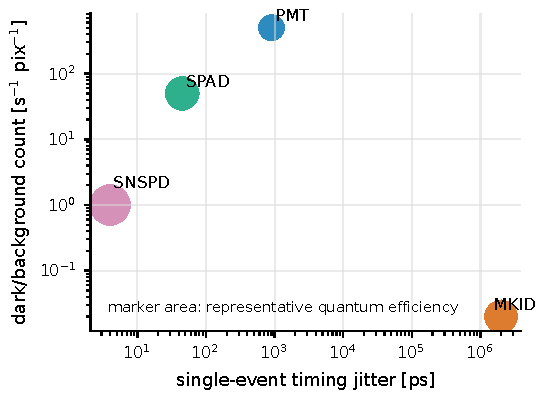
\includegraphics[width=0.72\linewidth]{figures/generated/chapter_06/ch06_detector_trade_space.pdf}
\caption{Typical operating regions of several classes of single-photon detection technology. The horizontal axis is the single-event timing jitter, the vertical axis a representative value of dark or background counts per pixel, and the point area indicates the representative quantum efficiency. PMTs suit large aperture, high flux, and ns-scale intensity interferometry; SPADs give tens-of-picoseconds timing but are limited by area and dead time; superconducting devices are strongest in low dark counts and picosecond timing but need a cryogenic system; energy-resolving detectors sacrifice timing resolution to gain the wavelength information of each photon.}
\label{fig:e13-detector-trade-space}
\end{figure}

One sentence to close this section: $\eta$ determines \emph{how many} photons become events, and thereby the "signal" in the signal-to-noise ratio; while the temporal properties of "when the event arrives and how soon the detector can fire again" determine whether the correlation structure in the event table is still faithful to the incident light field, which is exactly what the next three sections take apart.

\section{Timing jitter: why the correlation peak gets broadened}
\label{sec:e13-jitter}

Chapter~\ref{chap:e08} already foreshadowed: the detector's finite temporal response convolutionally broadens the narrow correlation peak and dilutes its height. Now we explain this thoroughly. The root of the problem is \textbf{timing jitter}: even if the same photon arrives at the same moment, the moment at which the detector output pulse is judged to be an "event" differs slightly each time, and is a random quantity. It is about tens of picoseconds for a SPAD, and can reach the ns-scale for a PMT plus electronic chain. Writing this random delay as a response function $h(t)$ (a normalized probability distribution describing "the distribution of recorded moments corresponding to the true arrival moment 0"), the observed event time is then the convolution of the true time with $h$.

For second-order correlation, each channel has its own response $h_1(t)$, $h_2(t)$, and the observed correlation excess is the convolution of the true celestial correlation with the combined response:
\begin{equation}
  C^{\rm obs}_{12}(\tau)
  =
  \int C^{\rm sky}_{12}(\tau')\,
  h_{12}(\tau-\tau')\,d\tau',
  \qquad
  h_{12}=h_1*h_2.
  \label{eq:e13-response-convolution}
\end{equation}
\begin{formulaexplain}
$C^{\rm sky}_{12}$ is the true celestial correlation, $C^{\rm obs}_{12}$ is the observed result; $h_1,h_2$ are the two channels' temporal responses, and $h_{12}$ is their convolution. The instrument "smears out" the narrow correlation peak.
\end{formulaexplain}
Here $C_{12}=g^{(2)}_{12}-1$ (dimensionless), $\tau,\tau'$ are in seconds, and $*$ is convolution. The physical picture is very plain: an infinitely narrow true correlation peak is of no use, because you simply do not know the \emph{exact} arrival moment of each photon, only that it falls within a fuzzy window of width about $\sigma$; the two fuzzy responses superpose, and the observed peak is broadened to the width of $h_{12}$.

To compute "how much broadening" precisely, use a very handy approximation: treat each response as a Gaussian. Here we single out a standard result: \emph{the convolution of two Gaussian functions is still a Gaussian, and the variances add}. Let $h_1$ be a Gaussian of width (variance) $\sigma_1^2$ and $h_2$ be a Gaussian of $\sigma_2^2$; then
\[
  h_{12}=h_1*h_2 \;\Longrightarrow\; \sigma_{12}^2=\sigma_1^2+\sigma_2^2 .
\]
Counting in the source's own width, the optical-path broadening, and the clock residual, if the terms are mutually independent the variances simply add (this is called "adding in quadrature," the general rule for the superposition of independent Gaussian broadenings):
\begin{equation}
  \sigma_{\rm obs}^2
  \simeq
  \sigma_{\rm sky}^2+\sigma_1^2+\sigma_2^2+\sigma_{\rm opt}^2+\sigma_{\rm clk}^2 .
  \label{eq:e13-jitter-budget}
\end{equation}
\begin{formulaexplain}
$\sigma_{\rm obs}$ is the observed peak width; $\sigma_{\rm sky}$ is the source's own width, $\sigma_1,\sigma_2$ are the two detectors' jitters, $\sigma_{\rm opt}$ is the optical-path broadening, and $\sigma_{\rm clk}$ is the clock residual. Independent Gaussian broadenings add in quadrature.
\end{formulaexplain}
Each term is an rms time width (seconds). $\sigma_{\rm sky}$ is the source's coherence time or pulse width, $\sigma_1,\sigma_2$ are the jitters of the detectors and electronic channels, $\sigma_{\rm opt}$ is the mirror isochronicity error (for example, the path-length differences among the different facets of a Davies--Cotton mirror), and $\sigma_{\rm clk}$ is the residual after aligning the clocks of the two stations. Here there is an important "order-of-magnitude landing": the coherence time $\tau_c$ of broadband visible light is as short as picoseconds (Chapter~\ref{chap:e02}), three orders of magnitude smaller than the ns-scale $\sigma_1,\sigma_2$, so in Eq.~\eqref{eq:e13-jitter-budget} the $\sigma_{\rm sky}$ term can almost be neglected: \emph{the observed peak width is almost entirely determined by the instrument}. VERITAS's mirror plus PMT pulse width make the intensity correlation peak describable by a Gaussian of $\sigma_\tau\simeq4\,{\rm ns}$, and the correlation peak of MAGIC-SII has a Gaussian width of about $2.2\,{\rm ns}$ \citep{2020NatAs...4.1164A,2024MNRAS.529.4387A}.

This brings a key consequence: \emph{when the peak width changes, the peak height changes too}. Because the "area" under the correlation peak (the total strength of the true correlation) is approximately conserved in the convolution, spreading it over a wider peak dilutes the peak height by the broadening factor. If the true peak width $\sigma_{\rm sky}\ll\sigma_{\rm obs}$, the observed peak height is lowered relative to the true peak height by roughly a factor of $\sigma_{\rm sky}/\sigma_{\rm obs}$. This is the quantitative source of what Chapter~\ref{chap:e08} called "the correlation peak being diluted by the temporal response," and it also explains why intensity interferometry strives so hard for high electronic bandwidth and a stable response function: the narrower the response, the less the peak-height dilution, and the easier it is to pick a peak of order $10^{-6}$ out of the noise.

\begin{figure}[tbp]
\centering
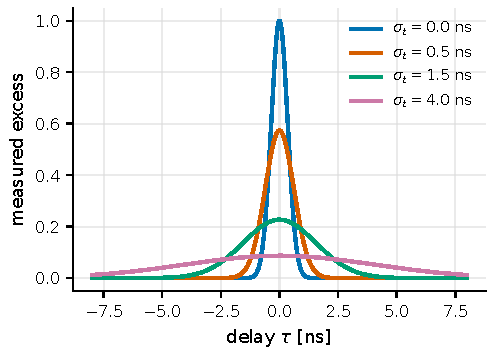
\includegraphics[width=0.72\linewidth]{figures/generated/chapter_06/ch06_detector_timing_response.pdf}
\caption{A finite temporal response broadens the narrow correlation peak and lowers its height. The curves keep the peak area approximately unchanged, changing only the rms jitter $\sigma_t$. When the true coherence time is far shorter than the ns-scale electronic response, the peak width is mainly determined by the instrument, and the peak height is diluted by the broadening factor; this is precisely why intensity interferometry needs high electronic bandwidth and a stable response function.}
\label{fig:e13-detector-timing-response}
\end{figure}

\section{Dead time and pile-up: why the recording rate saturates}
\label{sec:e13-deadtime}

Jitter changes the \emph{moment} of each event; dead time changes \emph{how many} events can be recorded. The \textbf{dead time} $\tau_d$ is a stretch of time after the detector fires during which it "catches its breath," blind to new photons. When photons come fast and dense, the dead time eats a large number of events, making the recording rate $r_{\rm rec}$ significantly lower than the true incident rate $r$: this is the count loss caused by \textbf{pile-up}. Here there is a subtle but important fork: does the dead time get "refreshed" by photons arriving during the dead time? Two answers give two models, and they must be told apart.

\paragraph{Non-paralyzable: the dead time is not refreshed}

First look at the \textbf{non-paralyzable} type. It assumes: after recording an event, the detector is dead for $\tau_d$; photons arriving during this time are all discarded, \emph{but the dead time is not extended}; once $\tau_d$ elapses, the detector immediately revives to await the next one. The derivation uses a "live-time ledger" method, done with no skipped steps.

Let the total observation duration be $T$, the true incident rate be $r$ (${\rm s}^{-1}$), and the total number of recorded events be $M$. Each recorded event brings $\tau_d$ of dead time, so the total dead time is $M\tau_d$, and hence the time the detector is truly "alive and responsive" is
\[
  T_{\rm live}=T-M\tau_d .
\]
The key to the non-paralyzable type is: only photons arriving during the live time are recorded, and during the live time photons arrive Poissonianly at the true rate $r$, so
\[
  M=r\,T_{\rm live}=r\,(T-M\tau_d).
\]
Gathering the terms containing $M$:
\[
  M=rT-rM\tau_d \;\Longrightarrow\; M+rM\tau_d=rT \;\Longrightarrow\; M(1+r\tau_d)=rT .
\]
Divide both sides by $T$ and write $r_{\rm rec}=M/T$ to obtain the recording rate:
\begin{equation}
  r_{\rm rec}=\frac{r}{1+r\tau_d}.
  \label{eq:e13-nonparalyzable}
\end{equation}
\begin{formulaexplain}
$r$ is the true incident rate, $r_{\rm rec}$ is the recording rate, and $\tau_d$ is the dead time. In the non-paralyzable type, photons within the dead time are discarded but do not extend the recovery window, so $r_{\rm rec}$ rises monotonically with $r$ and saturates to $1/\tau_d$.
\end{formulaexplain}
Read the limits of this formula. At low flux $r\tau_d\ll1$, the denominator approaches 1, $r_{\rm rec}\approx r(1-r\tau_d)$, and the loss is small; at high flux $r\tau_d\gg1$, $r_{\rm rec}\to 1/\tau_d$: the recording rate \emph{saturates} at an upper limit, the detector reporting at most one event every $\tau_d$, no matter how many more photons crowd in, but it never retreats.

\paragraph{Paralyzable: every photon refreshes the dead time}

Now look at the \textbf{paralyzable} type. It assumes: every new photon arriving during the dead time, though \emph{not recorded}, \emph{re-triggers} a fresh stretch of $\tau_d$ dead time. So a photon is recorded only when, at the moment it arrives, it has been \emph{empty for at least $\tau_d$} with no photons before it.

The derivation uses a standard result of the Poisson process: for a Poisson process of rate $r$, the time interval between two adjacent photons follows an exponential distribution, and \emph{the probability that the interval exceeds $\tau_d$ is $e^{-r\tau_d}$}. (This is the probability that "there is not a single photon in a window of length $\tau_d$," equal to the Poisson distribution taking 0: $P(0)=e^{-r\tau_d}$.) An arriving photon can be recorded if and only if the gap before it is greater than $\tau_d$. All photons arrive at rate $r$, and only the fraction whose "preceding gap $>\tau_d$" counts, so the recording rate is
\[
  r_{\rm rec}=r\times P(\text{preceding interval}>\tau_d)=r\,e^{-r\tau_d}.
\]
Written as a numbered formula:
\begin{equation}
  r_{\rm rec}=r\,e^{-r\tau_d}.
  \label{eq:e13-paralyzable}
\end{equation}
\begin{formulaexplain}
Likewise a dead-time model, but every arriving photon refreshes the recovery window. Hence $r_{\rm rec}$ reaches its maximum at $r\tau_d=1$, and thereafter \emph{decreases} as $r$ increases: at high flux the detector is almost continuously refreshed and reports no events.
\end{formulaexplain}
Read the limits: at low flux $r\tau_d\ll1$, $e^{-r\tau_d}\approx1-r\tau_d$, $r_{\rm rec}\approx r(1-r\tau_d)$, \emph{completely identical} to the non-paralyzable type at low flux, which is why the two models are hard to distinguish in weak light. But high flux is entirely different: differentiating $r_{\rm rec}=re^{-r\tau_d}$ with respect to $r$, $\frac{d r_{\rm rec}}{dr}=e^{-r\tau_d}(1-r\tau_d)$, which is zero at $r\tau_d=1$ (i.e. $r=1/\tau_d$), a maximum, with peak value $r_{\rm rec}^{\max}=1/(e\tau_d)\approx0.368/\tau_d$; beyond this, the photons are so dense that they continuously refresh the dead time, and the recording rate \emph{turns downward}, in the extreme leaving the detector almost paralyzed (hence the name of the model).

\paragraph{Comparison and orders of magnitude}

Reading the two formulas side by side, the physical difference in one sentence: the non-paralyzable type \emph{saturates} to $1/\tau_d$ at high flux, while the paralyzable type \emph{falls back} at high flux. This difference is critical experimentally: if you mistake a paralyzable type for a non-paralyzable one, you will severely overestimate the true rate at high count rates. So a real instrument must \emph{separately measure} which class it belongs to and what $\tau_d$ is, the method being to plot the curve of $r_{\rm rec}$ versus $r$ using a stable light source of adjustable intensity, and see whether it saturates or falls back.

Plug in numbers to get a feel for the magnitude. Take a typical dead time of a high-speed single-photon channel, $\tau_d=20\,{\rm ns}=2\times10^{-8}\,{\rm s}$:
\[
  r=10^7\,{\rm s^{-1}}:\quad r\tau_d=0.2,\quad
  r_{\rm rec}^{\rm non}=\frac{10^7}{1.2}\approx8.3\times10^6\,{\rm s^{-1}},
\]
that is, already a loss of about $17\%$; at the same incident rate the paralyzable type gives $r_{\rm rec}=10^7e^{-0.2}\approx8.2\times10^6\,{\rm s^{-1}}$, almost identical. Raising further to $r=10^8\,{\rm s^{-1}}$ ($r\tau_d=2$): the non-paralyzable type gives $r_{\rm rec}=10^8/3\approx3.3\times10^7\,{\rm s^{-1}}$, still climbing; the paralyzable type gives $r_{\rm rec}=10^8e^{-2}\approx1.35\times10^7\,{\rm s^{-1}}$, \emph{already over the peak and falling} (the peak occurs at $r=1/\tau_d=5\times10^7\,{\rm s^{-1}}$, where $r_{\rm rec}^{\max}\approx1.84\times10^7\,{\rm s^{-1}}$). SPADs commonly have dead times of tens of ns to a few hundred ns, energy-resolving detectors can reach the $100\,\mu{\rm s}$ scale, and modern TCSPC electronics can compress the channel dead time to 650 ps, though the detector pulse width and front-end electronics still limit the real high-flux capability \citep{2009A&A...508..531N,2013PASP..125.1348M,2020RScI...91a3108W}.

\begin{figure}[tbp]
\centering
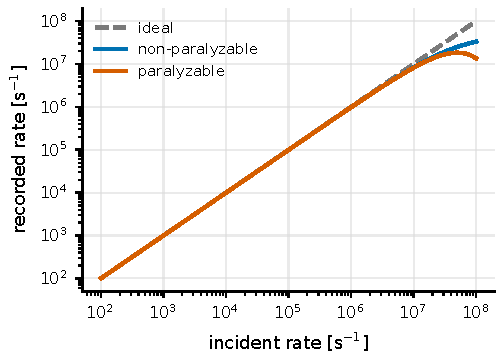
\includegraphics[width=0.72\linewidth]{figures/generated/chapter_06/ch06_deadtime_saturation.pdf}
\caption{As the incident count rate rises, dead time makes the recorded count rate deviate from the ideal straight line. The non-paralyzable type tends to the saturation value $1/\tau_d$, while the paralyzable type instead decreases at extremely high flux. The figure takes $\tau_d=20\,{\rm ns}$, representing the order of magnitude of a high-speed single-photon channel; a real instrument needs to measure $\tau_d$ and the model type separately using an adjustable-intensity light source.}
\label{fig:e13-deadtime-saturation}
\end{figure}

Dead time also hints at a trick commonly used in intensity interferometry: \textbf{split the light onto two independent detectors} for cross-correlation (the HBT approach, see Chapter~\ref{chap:e10}). Because the dead time is \emph{each detector's own}, the two detectors will not both miss a coincidence near zero delay because the other is in its dead time; this both raises the total count rate that can be tolerated and, as a bonus, suppresses the same-channel afterpulsing discussed in the next section \citep{1957RSPSA.242..300B,1996ApOpt..35.1956C,2020RScI...91a3108W}.

\section{Afterpulsing: short-delay false correlations the detector makes itself}
\label{sec:e13-afterpulse}

Dead time makes events \emph{fewer}, but afterpulsing makes events \emph{appear out of nothing}. In avalanche-type devices (SPAD, SiPM), an avalanche has some carriers "captured" by material defects (traps), which are released a while later and re-trigger a secondary pulse having nothing to do with celestial photons: this is the \textbf{afterpulse}. Its danger lies in this: these false pulses always follow closely behind the true pulse by a few ns to a few $\mu$s, falling exactly in the \emph{short-delay} interval we care about most, and forge a false peak in the autocorrelation, misread as "photons arriving in company."

Write it in rate form. Let the probability that each true event produces an afterpulse be $\epsilon_{\rm ap}$, and the delay of these afterpulses relative to the main pulse follow a normalized distribution $k_{\rm ap}(\tau)$; then the extra event rate is
\begin{equation}
  R_{\rm ap}(\tau)=\epsilon_{\rm ap}\,R_{\rm det}\,k_{\rm ap}(\tau),
  \qquad
  \int_0^\infty k_{\rm ap}(\tau)\,d\tau=1.
  \label{eq:e13-afterpulse}
\end{equation}
\begin{formulaexplain}
$R_{\rm ap}$ is the afterpulse contribution; $\epsilon_{\rm ap}$ is the probability that each true event produces an afterpulse; $R_{\rm det}$ is the true detection rate; $k_{\rm ap}$ is the normalized delay kernel. It describes the short-delay false correlation the detector \emph{makes itself}.
\end{formulaexplain}
Let us pin down each term. $\epsilon_{\rm ap}$ is dimensionless, ranging from $10^{-4}$ to $10^{-2}$ depending on the device and gating scheme; $R_{\rm det}$ is the detection rate given by Eq.~\eqref{eq:e13-detected-rate} (${\rm s}^{-1}$); $k_{\rm ap}(\tau)$ is in units of ${\rm s}^{-1}$ (because it integrates to unity over $\tau$), and its characteristic time ranges from ns to $\mu$s. The structure of the formula is "true event rate $\times$ single-afterpulse probability $\times$ delay distribution," very easy to remember.

How to distinguish it from a true signal? Two methods. First, do the autocorrelation \emph{on the same detector}, and you will see the afterpulse peak conspicuously appear at short delays; second, do the cross-correlation \emph{on two independent detectors}, and because the trap releases of detectors A and B are mutually independent and not synchronized, the afterpulses do not create coincidences in the cross-correlation and are thus greatly suppressed. This once again shows the double benefit of HBT beam-split cross-correlation: it both solves dead time and evades afterpulsing: the same light, split to two "mutually oblivious" detectors, so neither can use its own defects to contaminate the other's coincidence counts \citep{1957RSPSA.242..300B,1996ApOpt..35.1956C,2020RScI...91a3108W}.

\section{Clocks and synchronization: putting two telescopes on the same time axis}
\label{sec:e13-clock}

By now, the event table inside a single telescope has been built. But intensity interferometry and very-long-baseline timing need at least \emph{two} telescopes, and their respective event tables can only be correlated once placed on a \emph{common time axis}. This requires the clocks of the two stations to be aligned accurately enough. How accurate is enough? Here is a conversion that runs through the whole book, translating "timing precision" into "the distance light travels":
\begin{equation}
  \Delta\ell = c\,\Delta t .
  \label{eq:e13-lightpath}
\end{equation}
\begin{formulaexplain}
$\Delta t$ is the residual of aligning the two stations' clocks, $c$ is the speed of light, and $\Delta\ell$ is the distance light travels in this time. It directly converts "synchronized to how many picoseconds" into "equivalent to how many centimetres of path length."
\end{formulaexplain}
This formula is in fact the "time--path-length" correspondence used in Chapter~\ref{chap:e01}, only this time applied to clocks. Plug in numbers (CGS, $c=3\times10^{10}\,{\rm cm\,s^{-1}}$): $\Delta t=1\,{\rm ns}=10^{-9}\,{\rm s}$ corresponds to $\Delta\ell=30\,{\rm cm}$; $\Delta t=100\,{\rm ps}$ corresponds to $3\,{\rm cm}$; $\Delta t=1\,{\rm ps}$ corresponds to $0.3\,{\rm mm}$. So "synchronizing the two stations to the picosecond-nanosecond" is physically equivalent to "aligning the lengths of the two optical paths to the millimetre-centimetre", a very intuitive scale. Conversely, as long as you align the clocks to a few tens of picoseconds, a path-length difference within a few centimetres is absorbed by the clock.

There are two mainstream routes to achieving this synchronization. One is \textbf{GPS timing}: the satellite-broadcast pulse-per-second (PPS) gives each station a common absolute moment, complemented by a local rubidium clock for short-term stability; AquEYE/Iqueye use a rubidium clock plus GPS PPS to achieve a \emph{relative} time precision of about 100 ps rms and keep the \emph{absolute} UTC precision within $0.5\,{\rm ns}$ \citep{2009A&A...508..531N,2015SPIE.9504E..0CZ}. The other is \textbf{White Rabbit}: an Ethernet-based fibre synchronization protocol with precise phase measurement, which distributes one master clock via fibre to each station and compensates for the fibre length in real time; a 5 km fibre link test obtained a synchronization contribution of about 39 ps, which, converted by Eq.~\eqref{eq:e13-lightpath}, is equivalent to only about 1.2 cm of path-length residual \citep{2013NIMPA.725..187J,2020RScI...91a3108W}.

With a common clock, one must still subtract a larger, \emph{time-varying} term: the geometric delay. The same starlight arrives at the two stations at different moments, because the path lengths from the two stations to the source are unequal. For a pair of stations $a,b$:
\begin{equation}
  \Delta t_{\rm geo}(t)
  =
  \frac{\mathbf{B}_{ab}(t)\cdot\hat{\mathbf{s}}}{c},
  \qquad
  \mathbf{B}_{ab}=\mathbf{r}_b-\mathbf{r}_a .
  \label{eq:e13-geometric-delay}
\end{equation}
\begin{formulaexplain}
$\Delta t_{\rm geo}$ is the geometric delay between the two stations; $\mathbf B_{ab}$ is the baseline vector (given by the difference of the two stations' positions), $\hat{\mathbf s}$ is the unit vector of the source direction, and $c$ is the speed of light. It \emph{projects} the spatial baseline into the amount of time by which the two event tables must be shifted relative to each other.
\end{formulaexplain}
$\mathbf B_{ab}$ is in units of m, $\hat{\mathbf s}$ is dimensionless, the dot product $\mathbf B_{ab}\cdot\hat{\mathbf s}$ is the projected length of the baseline onto the source direction, and dividing by $c$ gives the time. Plug in numbers: a 100 m baseline gives at most $\Delta t_{\rm geo}=100/(3\times10^8)\approx333\,{\rm ns}$ (this maximum occurs when the source direction is parallel to the baseline, i.e. near the horizon; conversely, when the source is at the zenith and the baseline is nearly horizontal, the projection $\mathbf B_{ab}\cdot\hat{\mathbf s}\approx0$ and the geometric delay is near zero), and a 1 km baseline about $3.3\,\mu{\rm s}$, far larger than the picosecond-scale detector jitter, showing that the geometric delay is the \emph{largest} time term in the correlation, and must be subtracted first before aligning zero delay. More troublesome, it \emph{drifts with time}: Earth's rotation continuously changes the projected baseline, and a 100 m baseline drifts fastest near the zenith (culmination), with a delay change rate of about $\Omega_\oplus B/c\sim2.4\times10^{-11}\,{\rm s\,s^{-1}}$, where $\Omega_\oplus\approx7.3\times10^{-5}\,{\rm rad\,s^{-1}}$ is Earth's rotation angular velocity; this means about $24\,{\rm ps}$ of drift per second (about $25\,{\rm ns}$ accumulated over 17 minutes); for a picosecond-scale peak shape, this cannot be absorbed once and for all by a constant delay. VERITAS-SII applies a shifting time-lag correction for the geometric path per correlation frame, and MAGIC-SII applies a variable time-delay correction after the Pearson correlation \citep{2020NatAs...4.1164A,2024MNRAS.529.4387A}.

If one also wants to fold photons into a pulsar phase, or compare arrival times with other bands, the station time must be further converted to the \emph{Solar System barycenter} (SSB), adding a string of standard correction terms: the conversion from the local clock to coordinate time, the Roemer light-travel time (Earth's orbit around the Sun gives at most about $\pm500\,{\rm s}$), the Einstein gravitational/motional clock-rate correction, the Shapiro gravitational delay, and the atmospheric delay. Tempo2 has done these corrections to the ns level, and barycorrpy and Astropy provide Python-workflow interfaces \citep{2006MNRAS.369..655H,2006MNRAS.372.1549E,2018RNAAS...2....4K,2013A&A...558A..33A,2018AJ....156..123A}. These belong to the advanced content of absolute timing; for this chapter one need only remember: same-night intensity correlation looks at \emph{relative} delays, and only pulse phase and multi-messenger comparison need \emph{absolute} barycentric time.

\begin{figure}[tbp]
\centering
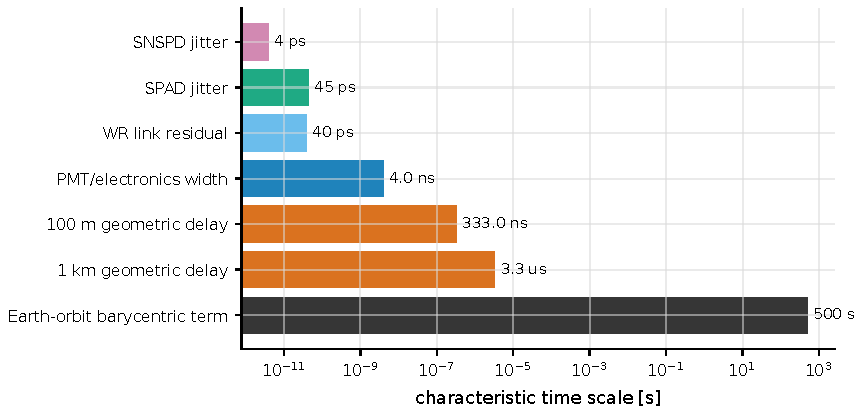
\includegraphics[width=0.84\linewidth]{figures/generated/chapter_06/ch06_time_budget.pdf}
\caption{The same event table simultaneously encounters time terms of picosecond, nanosecond, microsecond, and hundred-second scale. Detector jitter and the White Rabbit residual determine whether the correlation peak can keep its narrow shape; electronic and mirror responses determine the ns-scale intensity-interferometry peak width; the geometric delay is determined by the baseline length and source direction, and drifts with Earth's rotation; the Solar-System barycentric correction, though not a same-night peak-width term, is the absolute time basis for pulse phase, cross-night combination, and multi-messenger comparison.}
\label{fig:e13-time-budget}
\end{figure}

Writing all these delays into the calibrated event table, the raw counter time becomes a physical time comparable across stations:
\begin{equation}
  t^{\rm cal}_q =
  t^{\rm raw}_q
  +\Delta_{\rm clk}(t_q)
  +\Delta_{\rm elec}(a_q,d_q)
  +\Delta_{\rm det}(\lambda_q,d_q)
  -\frac{\mathbf{r}_{a_q}(t_q)\cdot\hat{\mathbf{s}}}{c}.
  \label{eq:e13-calibrated-time}
\end{equation}
\begin{formulaexplain}
$t_q^{\rm cal}$ is the corrected event time; $\Delta_{\rm clk},\Delta_{\rm elec},\Delta_{\rm det}$ respectively correct for the clock, electronic-link, and detector delays; the last term subtracts the geometric light-travel time. It places different stations on a common time axis.
\end{formulaexplain}
$\Delta_{\rm clk}$ is the offset of the local clock relative to the unified time scale (tens of picoseconds to ns), $\Delta_{\rm elec}$ is the fixed or slowly drifting delay of cables, amplifiers, discriminators, and ADC/TDC channels (commonly calibrated with a pulse source and loopback links), $\Delta_{\rm det}$ is the internal detector delay (which may depend on wavelength, bias, temperature, and pulse height), and the last term is exactly the geometric delay of Eq.~\eqref{eq:e13-geometric-delay}. This formula gathers all the delay terms of the previous sections into a unified time-calibration framework.

\section{The event-table fields: why every column must be kept}
\label{sec:e13-schema}

Now we can answer the most practical question from the start of the chapter: which fields should the event table store, exactly? The answer is to store in \emph{three layers}, and the raw layer must never be overwritten by post-processing.

The \textbf{raw layer} stores the quantities from Eq.~\eqref{eq:e13-raw-event} that are "closest to the electronics": the counter tick $n_q$, the telescope/station number $a_q$, the detector number $d_q$, the wavelength channel $c_q$, the polarization channel $p_q$, the quality flag $f_q$, and the weight $w_q$. Why can no column be omitted? Because each corresponds to a kind of \emph{choice you might still want to redo afterwards}: keeping $n_q$ lets you re-bin and re-do the delay correction; keeping $a_q,d_q$ lets you do \emph{cross}-correlation rather than autocorrelation (thereby evading dead time and afterpulsing); keeping $c_q$ lets you re-select frequency by wavelength afterwards; keeping $p_q$ lets you reconstruct polarization (polarization reconstruction is deferred to a later chapter, see Chapter~\ref{chap:e22}); keeping $f_q$ lets you trace the origin of an anomalous peak; keeping $w_q$ lets you do weighted analysis. Once this layer is compressed into a light curve, all these "redoings" become impossible.

The \textbf{calibrated layer} turns the raw ticks, via Eq.~\eqref{eq:e13-calibrated-time}, into physical time on a unified time axis, and adds physical quantities such as telescope attitude, wavelength, polarization, and weight. It is the product of "each analysis version," which can be updated as the calibration improves, but each time one must record which set of corrections was used. The \textbf{correlation-product layer} finally records the baseline, delay grid, bin width, correlation amplitude, rejection conditions, and covariance, that is, the "finished products" such as $g^{(2)}(\tau)$, $|V|^2$, or pulse arrival times.

How large is the data volume? It is determined by the event rate and the bytes per event:
\begin{equation}
  \dot{M}
  \simeq
  N_{\rm tel}\,N_{\rm ch}\,R_{\rm evt}\,N_{\rm byte}.
  \label{eq:e13-data-rate}
\end{equation}
\begin{formulaexplain}
$\dot M$ is the data rate; $N_{\rm tel}$ is the number of telescopes, $N_{\rm ch}$ the number of channels per telescope, $R_{\rm evt}$ the single-channel event rate, and $N_{\rm byte}$ the bytes per event. It estimates the storage pressure of an event table or waveform stream.
\end{formulaexplain}
$\dot M$ is in units of ${\rm byte\,s^{-1}}$. Plug in numbers: $N_{\rm tel}=4$, $N_{\rm ch}=8$, $R_{\rm evt}=10^6\,{\rm s^{-1}}$, $N_{\rm byte}=16$, then $\dot M\simeq4\times8\times10^6\times16=5.12\times10^8\,{\rm byte\,s^{-1}}\approx512\,{\rm MB\,s^{-1}}$. Continuous waveform sampling is even fiercer: VERITAS-SII continuously digitizes each telescope's PMT signal at 250 MS/s, about 250 MB/s per telescope, with the total data volume of an entire experiment reaching tens of TB \citep{2020NatAs...4.1164A}. As for storage format, the FITS BINTABLE extension suits long-term archiving and astronomical-software interoperability, while HDF5/Parquet suit high-throughput columnar filtering; Astropy provides interfaces for FITS, coordinate, and time processing, making it convenient to put the event table, time-scale conversion, and barycentric correction into the same Python analysis chain \citep{2010A&A...524A..42P,2013A&A...558A..33A,2018AJ....156..123A}.

The meaning of layering, in one sentence: it lets later readers regenerate light curves, $g^{(2)}(\tau)$, spatial visibilities, or pulse arrival times \emph{from the same raw data}, without having to guess which choices early scripts quietly made. Reproducibility is the highest principle of event-table design.

\section{The trade-off between spectral resolution and coherence time}
\label{sec:e13-spectral}

One last field deserves separate treatment: the wavelength channel $c_q$. Tagging each photon with a wavelength is not just for spectroscopy, but even more because \emph{the width of the wavelength channel directly determines the coherence time}, and the coherence time in turn determines the intrinsic width of the correlation peak. Recall Chapters~\ref{chap:e02} and~\ref{chap:e08}: the narrower the channel, the longer the phase memory of the electric field. Quantitatively, if the channel is approximately rectangular with central wavelength $\lambda$ and width $\Delta\lambda$:
\begin{equation}
  \tau_c
  \simeq
  \frac{1}{\Delta\nu}
  \simeq
  \frac{\lambda^2}{c\,\Delta\lambda}
  =
  \frac{R\,\lambda}{c},
  \qquad
  R=\frac{\lambda}{\Delta\lambda}.
  \label{eq:e13-coherence-time}
\end{equation}
\begin{formulaexplain}
$\tau_c$ is the coherence time; $\Delta\nu$ is the frequency bandwidth; $\lambda,\Delta\lambda$ are the central wavelength and wavelength bandwidth; $R=\lambda/\Delta\lambda$ is the spectral resolution. A narrow channel lengthens the phase memory, but lowers the single-channel photon rate.
\end{formulaexplain}
Do not skip the two middle steps. The first step $\tau_c\simeq1/\Delta\nu$ is the bandwidth--coherence-time relation of Chapter~\ref{chap:e02}. The second step converts $\Delta\nu$ into a wavelength quantity: differentiating $\nu=c/\lambda$, $|d\nu|=(c/\lambda^2)\,|d\lambda|$, so $\Delta\nu\simeq c\Delta\lambda/\lambda^2$, giving $\tau_c\simeq\lambda^2/(c\Delta\lambda)$. The third step recognizes $R=\lambda/\Delta\lambda$, so $\lambda^2/(c\Delta\lambda)=(\lambda/\Delta\lambda)(\lambda/c)=R\lambda/c$. All three steps are identity transformations, with no extra approximation.

Plug in numbers ($\lambda=500\,{\rm nm}$): $R=100\Rightarrow\tau_c\simeq100\times500\times10^{-9}/(3\times10^8)\approx0.17\,{\rm ps}$; $R=10^4\Rightarrow\tau_c\simeq17\,{\rm ps}$; $R=10^5\Rightarrow\tau_c\simeq170\,{\rm ps}$. Note: even at $R=10^5$, $\tau_c$ is still shorter than the ns response of most PMTs/electronic chains, so by the conclusion of Section~\ref{sec:e13-jitter}, the actual correlation peak width is \emph{still determined by the instrument}; raising $R$ lengthens the phase memory (thereby affecting the ratio of electronic to optical bandwidth in the peak \emph{height}), rather than making the peak narrower.

Hence the final trade-off of the chapter. Raising $R$ (using a narrower filter) lengthens $\tau_c$ and makes the coherence "purer," but at the same time lowers the single-channel photon rate by about $1/R$ (the narrower the bandwidth, the fewer photons come in). To have both, one must \emph{read out more wavelength channels simultaneously} to make up the total flux: multi-channel TCSPC can treat different wavelengths as independent inputs and output a single time-ordered data stream; whereas the SII systems of MAGIC and VERITAS go the other way, choosing a few wide filter channels to gain a higher photon rate: VERITAS uses a filter centred at 416 nm with an effective width of 13 nm, and MAGIC uses an interference filter of 425 nm and 26 nm \citep{2020NatAs...4.1164A,2024MNRAS.529.4387A,1974iiia.book.....H}. Choosing wide or narrow depends on the science goal: to measure a stellar diameter, a wide channel that boosts the signal-to-noise ratio is fine; but to study emission lines, absorption lines, or the velocity structure of a rapid rotator, wavelength-resolved correlation can directly give "how the spatial information varies with velocity," and then the price of a narrow channel is worth paying.

\begin{figure}[tbp]
\centering
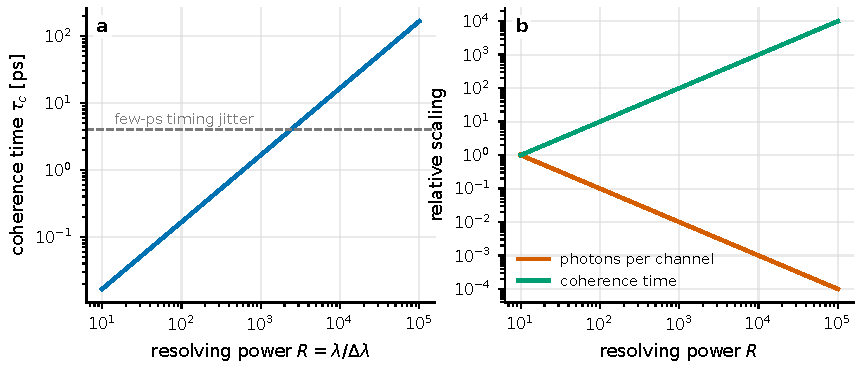
\includegraphics[width=0.92\linewidth]{figures/generated/chapter_06/ch06_spectral_resolution_coherence.pdf}
\caption{The order-of-magnitude relation between spectral resolution and coherence time. The left panel fixes $\lambda=500\,{\rm nm}$ and shows $\tau_c\simeq R\lambda/c$ growing linearly with resolution; the right panel shows the single-channel photon rate falling roughly as $1/R$ while the coherence time increases with $R$. The dependence of ideal intensity-interferometry signal-to-noise on optical bandwidth partly cancels, but a real instrument is further limited by filter shape, detector response, background, and electronic bandwidth.}
\label{fig:e13-spectral-resolution-coherence}
\end{figure}

\section{Chapter Summary}
\label{sec:e13-summary}

\begin{itemize}
  \item \textbf{A photon must pass several checkpoints to become an event.} The quantum efficiency $\eta$ determines "how many photons become events" (Eq.~\eqref{eq:e13-detected-rate}); PMTs offer large area and high gain, SPADs/SiPMs offer single-photon picosecond timing but are limited by area, dead time, and afterpulsing; each has its trade-offs.
  \item \textbf{Jitter broadens the correlation peak and dilutes its height.} The observed peak is the convolution of the true peak with the instrument response (Eq.~\eqref{eq:e13-response-convolution}); independent Gaussian broadenings add in quadrature, $\sigma_{\rm obs}^2=\sum\sigma_i^2$ (Eq.~\eqref{eq:e13-jitter-budget}). Visible-light $\tau_c\sim$ps is far smaller than the ns-scale response, so the peak width is almost entirely determined by the instrument, and the peak height is diluted by $\sim\sigma_{\rm sky}/\sigma_{\rm obs}$, echoing Chapter~\ref{chap:e08}.
  \item \textbf{Dead time saturates the recording rate, and comes in two types.} The non-paralyzable type $r_{\rm rec}=r/(1+r\tau_d)$ (Eq.~\eqref{eq:e13-nonparalyzable}) saturates at high flux to $1/\tau_d$; the paralyzable type $r_{\rm rec}=re^{-r\tau_d}$ (Eq.~\eqref{eq:e13-paralyzable}) peaks at $r\tau_d=1$ and then falls back. They coincide at weak light but differ vastly at strong light, so the type must be measured.
  \item \textbf{Afterpulsing forges false short-delay peaks.} The afterpulse rate $R_{\rm ap}=\epsilon_{\rm ap}R_{\rm det}k_{\rm ap}(\tau)$ (Eq.~\eqref{eq:e13-afterpulse}) falls in the crucial short-delay region. Splitting to two independent detectors for cross-correlation resolves dead time and afterpulsing at once.
  \item \textbf{Clock synchronization is equivalent to aligning path lengths.} $\Delta\ell=c\Delta t$ (Eq.~\eqref{eq:e13-lightpath}): 100 ps $\leftrightarrow$ 3 cm, 1 ns $\leftrightarrow$ 30 cm. GPS/White Rabbit align the two stations to tens of picoseconds; the geometric delay $\Delta t_{\rm geo}=\mathbf B\cdot\hat{\mathbf s}/c$ (Eq.~\eqref{eq:e13-geometric-delay}) is the largest (about 333 ns for a hundred-metre baseline) and drifts with Earth's rotation, and must be subtracted frame by frame.
  \item \textbf{The event table has three layers, preserving the raw information.} The raw layer cannot be overwritten, the calibrated layer can be iterated, and the correlation-product layer delivers finished products; each field corresponds to a "redoing you might still want afterwards." Reproducibility is the highest principle.
  \item \textbf{Spectral resolution and coherence time trade off against each other.} $\tau_c\simeq R\lambda/c$ (Eq.~\eqref{eq:e13-coherence-time}): the larger $R$, the longer the coherence time, but the single-channel photon rate falls by about $1/R$. Choosing wide or narrow depends on whether you are measuring a diameter or studying velocity structure.
\end{itemize}

\noindent\textbf{Questions to Ponder.} (1) If a SPAD's dead-time curve first rises and then falls at high flux, which type is it more likely to be? Based on this, how do you infer $\tau_d$ backwards? (2) Aligning two stations' clocks to 50 ps is equivalent to aligning how long a path length? Is this large or small relative to the geometric delay of a 100 m baseline? (3) If you raise $R$ from 100 to $10^4$, by how many times does the coherence time increase, and to about what fraction does the single-channel photon rate fall? What should be done to preserve the total flux?

\chapter{Correlators and Event-Table Data Analysis}
\label{chap:e14}

\begin{chapteropening}
In the previous chapter (Chapter~\ref{chap:e13}), the telescope wrote every photon candidate as one line of record: when it arrived, from which station, through which detector channel, at what wavelength, in what polarization. Over a single night, such records may number in the billions of lines; they lie quietly on disk, being in themselves neither an angular diameter nor a $g^{(2)}$, just a heap of time stamps.

What this chapter answers is precisely the process that lies between "a heap of events" and "a trustworthy curve": how do you turn these billions of time stamps into a $|V|^2$ or $g^{(2)}$ with error bars, one that is reproducible and can be taken away to fit physical models? We will follow one main thread: first translate the event table into a probabilistic model (write the likelihood), then define the correlation estimator and normalize it, then solve "can it be computed in finite time" (the computational scaling of the correlator), and finally the most underestimated link in all of the book's data analysis: where the errors come from, and why systematic error is so often the ceiling. The delay histogram given in Chapter~\ref{chap:e08}, and the Fisher-information language given in Chapter~\ref{chap:e12}, will here be genuinely put to use.
\end{chapteropening}

\section{From the event table to a probabilistic model}
\label{sec:e14-model}

Let us first agree on notation. Denote a calibrated event table as a whole by a dataset
\begin{equation}
  \mathcal{D}
  =
  \left\{
  t_q,\ a_q,\ d_q,\ c_q,\ p_q,\ w_q,\ f_q
  \right\}_{q=1}^{N_{\rm evt}} ,
  \label{eq:e14-data}
\end{equation}
\begin{formulaexplain}
$\mathcal D$ is the entire calibrated event table; each event $q$ carries a time $t_q$, station $a_q$, detector $d_q$, spectral channel $c_q$, polarization $p_q$, weight $w_q$, and quality flag $f_q$; $N_{\rm evt}$ is the total number of events. It is the raw "ingredient" of every estimator that follows.
\end{formulaexplain}
Here $t_q$ is the arrival moment on a unified time scale (units of s, with typical precision reaching nanoseconds or even tens of picoseconds), $a_q,d_q,c_q,p_q$ are all integer channel numbers (dimensionless), $w_q$ is the weight (dimensionless), and $f_q$ is the quality bit flagging whether this event is "clean." How these fields arise, how the clock is calibrated, and how the format is defined were the content of the previous chapter (Chapter~\ref{chap:e13}); this chapter starts directly from "the table already in hand."

The first step of the analysis is not to draw a plot, but to write down a \textbf{selection function}, which decides which events participate in the subsequent computation:
\begin{equation}
  S_q = S(t_q,a_q,d_q,c_q,p_q,f_q),
  \qquad
  S_q\in\{0,1\}\ \text{or}\ [0,1] .
  \label{eq:e14-selection}
\end{equation}
\begin{formulaexplain}
$S_q$ is the selection/weight of the $q$-th event; taking 0 or 1 means rejection or retention, while taking a continuous value in $[0,1]$ means a weighting due to exposure, dead time, background, or efficiency. It turns "manual point selection" into a rule that can be rerun.
\end{formulaexplain}
Why be so formal? Imagine a channel event rate of $10^{6}\,\mathrm{s^{-1}}$: a one-hour observation is $3.6\times10^{9}$ events. No one can "watch the plot and manually delete a few bad points", that is neither feasible nor reproducible. The selection function must be automatically regenerable from metadata (cloud cover, PMT current, dead-time flags, thresholds), so that the light-curve, correlation, and fitting layers all use the same criteria. When Chapter~\ref{chap:e15} does the error budget it will repeatedly emphasize: all systematic tests must be performed under the same set of $S_q$.

\paragraph{Unbinned data: the inhomogeneous Poisson point process}

Events are discrete points on the time axis, and the most natural model is the \textbf{inhomogeneous Poisson point process}: the instantaneous event rate at a given moment and channel is $\lambda(t,\bm{x}\mid\bm{\theta})$, where $\bm x$ packages the labels of channel, wavelength, polarization, sky position, etc., and $\bm\theta$ are the physical parameters we ultimately want to estimate. Chapter~\ref{chap:e03} explained: in a Poisson process, the probability of "one event occurring in a very short stretch of time" is proportional to the rate times the duration, and the stretches are mutually independent. We use exactly this to build up the likelihood step by step.

Cut the whole observation into many extremely narrow cells $\Delta t$, so narrow that each cell contains at most one event. The probability that the $i$-th cell "has one event" is about $\lambda_i E_i\,\Delta t$ ($E_i$ is the effective exposure of this cell), and the probability of "no event" is about $1-\lambda_i E_i\,\Delta t\approx e^{-\lambda_i E_i\Delta t}$. The likelihood of the whole observation is the product over all cells: occupied cells contribute $\lambda E\Delta t$, and empty cells contribute $e^{-\lambda E\Delta t}$. Take the logarithm:
\[
  \ln L
  =\sum_{q:\,S_q>0}\ln\!\big(\lambda(t_q,\bm x_q)\,E_q\,\Delta t\big)
   -\sum_{\text{all cells}}\lambda_i E_i\,\Delta t .
\]
Let $\Delta t\to0$: in the first term, $\ln\!\big(\lambda E_q\,\Delta t\big)=\ln\lambda+\ln E_q+\ln\Delta t$ can be split, where $\ln\Delta t$ is the binning width and $\ln E_q$ is the instrument/exposure term of this cell, both independent of the parameters $\bm\theta$ to be estimated and thus dropped together as constants in the fit (note that the exposure $E$ itself does not vanish; it is fully retained in the integral of the second term), so the first term keeps only $\ln\lambda$; the second sum becomes an integral. Hence
\begin{equation}
  \ln L(\bm\theta)
  =
  \sum_{q:\,S_q>0}\ln\lambda(t_q,\bm x_q\mid\bm\theta)
  -\int_{\mathcal T}\lambda(t,\bm x\mid\bm\theta)\,E(t,\bm x)\,dt\,d\bm x .
  \label{eq:e14-point-likelihood}
\end{equation}
\begin{formulaexplain}
$\ln L$ is the point-process log-likelihood. The first term scores the model rate at each real event: an event landing in a high-rate region gains points. The second term is the total number of events the model predicts over the effective exposure $E$: the model cannot merely spike at the events, it must also explain why there are no events elsewhere.
\end{formulaexplain}
Let us spell out each symbol: $\lambda$ has units of $\mathrm{s^{-1}}$ (or $\mathrm{s^{-1}\,channel^{-1}}$), $E(t,\bm x)$ is dimensionless or carries an area/efficiency factor, holding the real losses of bad weather, dead time, channel on/off, filter transmission, and observation window. The most important teaching point of this formula is its "balance": making the rate high only at the events cannot fool the second term, because the second term deducts points for predicting too many events. This is precisely the Cash statistic in astronomy, and at low counts one cannot get away with the symmetric $\sqrt N$ error \citep{1979ApJ...228..939C,1986ApJ...303..336G}.

\begin{figure}[tbp]
\centering
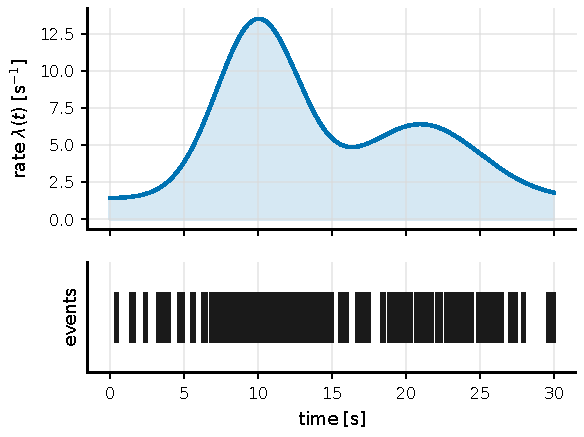
\includegraphics[width=0.72\linewidth]{figures/generated/chapter_07/ch07_poisson_likelihood.pdf}
\caption{The picture of an inhomogeneous Poisson process. The upper panel is the instantaneous rate $\lambda(t)$ fluctuating with time, and the lower panel is a string of events randomly "dropped" by this rate. The likelihood~\eqref{eq:e14-point-likelihood} uses both "events landing at high rate" and "the integrated rate over the whole stretch"; if the events are merely re-binned into a light curve, part of the time information is lost, especially for rapid variability or uneven exposure.}
\label{fig:e14-poisson}
\end{figure}

\paragraph{Binned data: degenerating to per-cell Poisson}

If we first bin the events into time cells, spectral channels, or delay cells, the point-process likelihood degenerates into the \textbf{binned Poisson likelihood} that everyone knows. The $i$-th cell observes $d_i$ events, the model predicts $m_i(\bm\theta)$, and the Poisson probability is $P(d_i)=e^{-m_i}m_i^{d_i}/d_i!$ (see Chapter~\ref{chap:e03}). The cells are independent; take the logarithm and sum:
\begin{equation}
  \ln L
  =\sum_i\Big[\,d_i\ln m_i(\bm\theta)-m_i(\bm\theta)-\ln(d_i!)\,\Big] .
  \label{eq:e14-binned-poisson}
\end{equation}
\begin{formulaexplain}
$d_i$ is the observed count of the $i$-th cell, $m_i$ the model count, both dimensionless. This is the likelihood usable by light curves, spectral channels, and delay histograms alike; it innately preserves the asymmetric statistics at low counts and does not pretend the errors are Gaussian.
\end{formulaexplain}
When a cell's count $d_i\gtrsim20$ and the model is not near a boundary, the Poisson can be approximated as Gaussian with error bars of about $\sqrt{d_i}$; but when a cell has only a few counts (as the signal window of a delay histogram often does), one must stay with Eq.~\eqref{eq:e14-binned-poisson}. There is another pitfall to mention in advance: when the model adds a component "whose strength must be nonnegative" (for example, "is there a correlation peak or not"), zero strength falls on the parameter boundary, the likelihood-ratio test no longer follows the nominal $\chi^2$ distribution, and the significance must be calibrated by simulation or posterior predictive checks \citep{2002ApJ...571..545P}. For slowly varying backgrounds and burst screening, Bayesian Blocks adaptively cuts the time axis into several "constant-rate segments," with data gaps entering through the effective exposure (live time) rather than being mistaken for "no events" \citep{2013ApJ...764..167S}; but the final physical parameters should still return to an explicit likelihood.

\section{How two streams of events grow a correlation peak}
\label{sec:e14-corr}

The core action of intensity interferometry is to compare the event arrival times of two stations $a,b$. Chapter~\ref{chap:e08} already obtained the idea of the delay histogram from $g^{(2)}$; here we cast it into an estimator that can run on real event tables.

The first step is to compute the \textbf{corrected time difference}. The raw time difference is mixed with the geometric delay and the instrument delay, which must be subtracted first:
\begin{equation}
  \tau_{ij}^{ab}
  =
  t_{j,b}^{\rm cal}-t_{i,a}^{\rm cal}
  -\Delta t_{\rm geo}^{ab}(t_i,\hat{\bm s})
  -\Delta t_{\rm inst}^{ab}(t_i) .
  \label{eq:e14-delay}
\end{equation}
\begin{formulaexplain}
$\tau_{ij}^{ab}$ is the corrected delay of two events at stations $a,b$; $t^{\rm cal}$ is the calibrated time, $\Delta t_{\rm geo}$ subtracts the geometric delay (the wavefront reaches the near telescope first), and $\Delta t_{\rm inst}$ subtracts the residual instrument delay of the two paths. It decides which delay cell this pair of events falls into.
\end{formulaexplain}
Why can the geometric delay not be neglected? For a 100 m baseline, the maximum time difference of the wavefront reaching the two telescopes is about $100/c\approx333\,\mathrm{ns}$; for a 1 km baseline it is $3.3\,\mu\mathrm{s}$. If the delay cell width is $\Delta\tau=4\,\mathrm{ns}$, then a geometric delay wrong by even one cell pushes the correlation peak away from zero delay and it vanishes outright. Furthermore, Earth is rotating, the projected baseline direction $\hat{\bm s}$ changes with time, and at tens-of-picoseconds precision the geometric delay must be continuously updated within very short time blocks \citep{2006MNRAS.369..655H,2006MNRAS.372.1549E,2018RNAAS...2....4K,2020NatAs...4.1164A}.

The second step is to count pairs: count all event pairs whose delay falls within the $k$-th cell $\tau_k\pm\Delta\tau/2$:
\begin{equation}
  C_{ab,k}
  =\sum_{i\in a}\sum_{j\in b}
  S_iS_j\,
  \mathbf 1\!\left[\tau_k-\tfrac{\Delta\tau}{2}\le\tau_{ij}^{ab}<\tau_k+\tfrac{\Delta\tau}{2}\right] .
  \label{eq:e14-paircount}
\end{equation}
\begin{formulaexplain}
$C_{ab,k}$ is the number of event pairs in the $k$-th delay cell; $S_iS_j$ weights each pair, and the indicator function $\mathbf 1[\cdot]$ picks only the pairs whose delay falls within that cell. It is one bar of the delay histogram, dimensionless.
\end{formulaexplain}

\paragraph{Normalization: the correlation peak is a faint excess on a background}

How tall one bar is has no meaning in itself, because even if the two streams were completely unrelated, pure randomness would still throw up a heap of "accidental coincidences." Assume the two streams are independent and their rates are approximately steady over the live time; the expectation of accidental coincidences can be estimated thus: stream $a$ has $R_aT_{\rm live}$ events in total, and each event has a probability of about $R_b\Delta\tau$ of "hitting" a stream-$b$ event within the delay cell $\Delta\tau$, and multiplying the two:
\begin{equation}
  B_{ab,k}\simeq R_aR_b\,\Delta\tau\,T_{\rm live} .
  \label{eq:e14-accidental}
\end{equation}
\begin{formulaexplain}
$B_{ab,k}$ is the accidental-coincidence background; $R_a,R_b$ (units $\mathrm{s^{-1}}$) are the two streams' mean rates, $\Delta\tau$ is the cell width, and $T_{\rm live}$ is the integration time after subtracting bad time. It is the number of accidental pairs that each cell should have "in the absence of celestial correlation."
\end{formulaexplain}
Plug in real numbers to feel the magnitude: take $R_a=R_b=10^{7}\,\mathrm{s^{-1}}$, $\Delta\tau=1\,\mathrm{ns}$, $T_{\rm live}=3600\,\mathrm{s}$, giving $B\approx10^{7}\times10^{7}\times10^{-9}\times3600\approx3.6\times10^{8}$. The background is as high as hundreds of millions of pairs, and the celestial correlation is only a tiny excess of order $10^{-6}$--$10^{-4}$ on top of it \citep{1974iiia.book.....H,2020NatAs...4.1164A,2024MNRAS.529.4387A}. Putting the two numbers together makes it clear: the signal $\approx3.6\times10^{8}\times10^{-4}\approx3.6\times10^{4}$ pairs, while the Poisson fluctuation of the background $\approx\sqrt{B}\approx1.9\times10^{4}$: after an hour the signal-to-noise ratio is only $\sim2$. Why intensity interferometry must integrate for tens of hours is written right here.

Dividing the bar by the background gives the normalized second-order correlation estimator and its excess:
\begin{equation}
  \widehat g^{(2)}_{ab}(\tau_k)=\frac{C_{ab,k}}{B_{ab,k}},
  \qquad
  \widehat C_{ab}(\tau_k)=\widehat g^{(2)}_{ab}(\tau_k)-1 .
  \label{eq:e14-g2}
\end{equation}
\begin{formulaexplain}
$\widehat g^{(2)}$ is the normalized second-order correlation, and $\widehat C_{ab}$ is the excess relative to the random background (dimensionless). The intensity-interferometry signal is hidden in this tiny excess after subtracting 1.
\end{formulaexplain}
In practice one rarely uses the analytic background of Eq.~\eqref{eq:e14-accidental} directly, but estimates $B$ using a \textbf{time-shift background}: shift stream $b$ as a whole by $\Delta T_{\rm shift}$, the shift being far larger than the correlation-peak width (so the true signal is moved away) yet far smaller than the slow-variation time of gain and rate (so the background structure is preserved). Averaging over multiple positive and negative shifts simultaneously gives the background mean and the background uncertainty. In addition there are stand-ins such as off-source (estimating skyglow, dark current), off-band (spectral-line science), and wrong-polarization (searching for crosstalk). VERITAS-SII rejects high-frequency electronic noise and low-PMT-current frames on 1-second correlation frames, then weights and averages the frames after the geometric-delay correction; MAGIC-SII uses the DC readings of the signal pixel and background pixel together to correct for night-sky light \citep{2020NatAs...4.1164A,2024MNRAS.529.4387A}.

\begin{figure}[tbp]
\centering
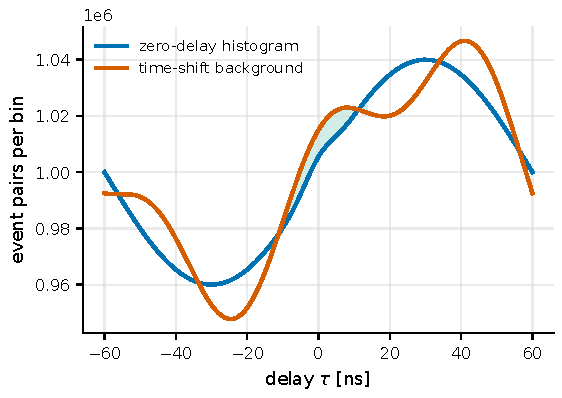
\includegraphics[width=0.72\linewidth]{figures/generated/chapter_07/ch07_time_shift_background.pdf}
\caption{The structure of time-shift background estimation. The blue curve is the event-pair histogram near zero delay, the orange curve is the accidental-coincidence background obtained by shifting one stream as a whole to a nonphysical delay, and the green region is the excess of the central peak relative to the time-shift background. This method preserves the slowly varying rate, bad time, and background structure, but the shift must be far larger than the instrument response width and the celestial correlation width.}
\label{fig:e14-timeshift}
\end{figure}

\paragraph{The continuous-waveform version: Pearson correlation}

If the hardware gives not discrete events but a continuously sampled voltage/current waveform (as MAGIC-SII does), the basic quantity becomes the \textbf{Pearson correlation coefficient}:
\begin{equation}
  \rho_{ab}(\tau_k)
  =\frac{\sum_n\big[x_a(t_n)-\bar x_a\big]\big[x_b(t_n+\tau_k)-\bar x_b\big]}
        {\sqrt{\sum_n\big[x_a(t_n)-\bar x_a\big]^2\;\sum_n\big[x_b(t_n)-\bar x_b\big]^2}} .
  \label{eq:e14-pearson}
\end{equation}
\begin{formulaexplain}
$\rho_{ab}$ measures the synchronous fluctuation of the two demeaned waveforms; $x_a,x_b$ are the sampled voltages/currents, and $\bar x$ is each one's mean. The denominator normalizes so that $\rho\in[-1,1]$; but it still mixes star, night-sky light, and electronic noise, and needs further calibration to become $|V|^2$.
\end{formulaexplain}
The Pearson correlation is very convenient to compute in real time in hardware (just demean, multiply, accumulate), but what it measures is a mixture of three fluctuations, and it must be calibrated with the DC current, background pixels, and zero baseline to be converted into the physical squared visibility $|V|^2$ \citep{2024MNRAS.529.4387A}. One last engineering detail: the cell width $\Delta\tau$ must be chosen together with the correlation-peak width and the time-stamp quantization: too wide dilutes the peak height, too narrow makes adjacent cells strongly correlated and inflates the computation for nothing; VERITAS-SII takes a correlation lag interval of 4 ns with a peak width also of about 4 ns, whereas a TDC of tens of picoseconds can cut the cells much finer, provided the geometric delay, instrument response, and clock residual are of equal precision \citep{2020NatAs...4.1164A,2020RScI...91a3108W,2009A&A...508..531N}.

\section{How the correlator finishes computing within a single night}
\label{sec:e14-scaling}

Now we face a purely engineering problem: that double sum in Eq.~\eqref{eq:e14-paircount}, can it really be computed?

\textbf{The most naive pair-by-pair method.} The two streams have $N_a,N_b$ events, and a full comparison is $N_aN_b$ differences; for the autocorrelation of the same stream, it is $N(N-1)/2$ pairs. Take $N_a=N_b=10^{9}$; that is $10^{18}$ differences, even at a billion per second ($10^{9}\,\mathrm{s^{-1}}$, roughly the realistic single-core speed), it would take $10^{18}/10^{9}=10^{9}\,\mathrm s\approx30$ years. The pair-by-pair method is fit only for small-sample teaching checks.

\textbf{The sorted-window method.} The true correlation peak lies only within a very narrow delay window, and there is no need to compare event pairs separated by several seconds. Sort both streams by time and look for pairs only within a sliding window $|t_{j,b}-t_{i,a}|\le W$; the number of candidate pairs to check is about
\begin{equation}
  N_{\rm pair}^{\rm win}\simeq 2W\,R_b\,N_a .
  \label{eq:e14-window}
\end{equation}
\begin{formulaexplain}
$N_{\rm pair}^{\rm win}$ is the number of candidate pairs the window method must check; $W$ (units s) is the maximum delay-window half-width, $R_b$ is the second stream's rate, and $N_a$ is the first stream's event count. A finite window brings the complexity from $N^2$ back to nearly linear.
\end{formulaexplain}
Substitute $W=100\,\mathrm{ns}$, $R_b=10^{6}\,\mathrm{s^{-1}}$, $N_a=10^{9}$: the candidate pairs are about $2\times10^{-7}\times10^{6}\times10^{9}=2\times10^{8}$, a full ten orders of magnitude fewer than the full double loop, and a workstation can sweep through them in a few minutes. Moreover, the sorted-window method preserves every event's full labels (wavelength, polarization), making re-selection afterwards convenient.

\textbf{FFT correlation: the XF and FX arrangements.} If the events or waveforms have already been placed into uniform time cells, one can use the fast Fourier transform to turn the time-domain cross-correlation into a frequency-domain multiplication:
\begin{equation}
  c_{ab}[k]
  =\mathcal F^{-1}\!\Big[\mathcal F\{x_a[n]\}^{*}\,\mathcal F\{x_b[n]\}\Big]_k .
  \label{eq:e14-fft}
\end{equation}
\begin{formulaexplain}
$c_{ab}[k]$ is the discrete cross-correlation; $\mathcal F,\mathcal F^{-1}$ are the forward/inverse discrete Fourier transforms, and the asterisk is complex conjugation. It replaces cell-by-cell multiply-accumulate ($O(N_{\rm bin}^2)$) with a single frequency-domain multiplication ($O(N_{\rm bin}\log N_{\rm bin})$), $N_{\rm bin}$ being the number of uniform time cells (a separate symbol is introduced here; do not confuse it with the $M$ denoting the number of time-shift backgrounds in the later error budget).
\end{formulaexplain}
Here appear the two kinds of correlator division of labour familiar from radio arrays: the \textbf{XF} type first does the cross-correlation (correlate, obtaining the delay-domain $c_{ab}[k]$) and then Fourier-transforms into a spectrum; the \textbf{FX} type does the reverse, first doing one FFT (Fourier) per stream, then cross-multiplying the streams pairwise in each frequency channel. Why is FX preferred once there are many stations? Because the FFT is a "once per stream" cost, growing linearly with the number of telescopes $N_{\rm tel}$; whereas the pairwise-multiply step is $O(N_{\rm tel}^{2})$ in either arrangement and cannot be avoided. When there are few stations (today's intensity-interferometry arrays often have only 2--4, so the number of pairs $N(N-1)/2$ is small), the bottleneck is not the number of pairs at all, but the \textbf{number of time samples each pair must swallow}: this is the correlator's real heavy lifting.

\begin{figure}[tbp]
\centering
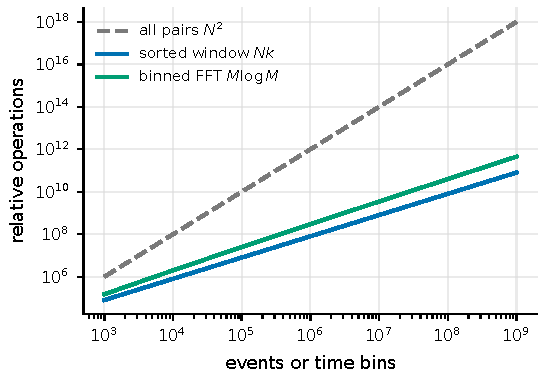
\includegraphics[width=0.72\linewidth]{figures/generated/chapter_07/ch07_correlator_scaling.pdf}
\caption{The operation-count scaling of three classes of correlation computation. The full pair-by-pair double loop grows wildly as $N^2$, suited only to small samples or teaching checks; the sorted window compares only pairs within a finite delay and is nearly linear; the FFT correlation after uniform binning grows as $N_{\rm bin}\log N_{\rm bin}$, suited to continuous sampling and real-time monitoring. The actual speed is further governed by memory bandwidth, I/O, GPU/FPGA data layout, and quality filtering.}
\label{fig:e14-scaling}
\end{figure}

\textbf{Real-time, dead-time-free hardware correlation.} VERITAS-SII streams the continuous PMT waveform to disk and then correlates offline with an FPGA; MAGIC-SII instead uses a GPU to compute all four-channel pairwise correlations in real time during the observation \citep{2020NatAs...4.1164A,2024MNRAS.529.4387A}. Continuous-waveform correlation has one advantage that single-photon counting cannot match: it does not rely on "trigger-and-reset per photon," and therefore has no dead-time blind spot of the kind a single-photon detector has after each count, and can compute the whole stretch of fluctuation into the correlation uninterruptedly; this is especially important for intensity interferometry with a signal of only $10^{-6}$--$10^{-4}$, where any time thrown away is signal-to-noise thrown away for nothing. Multi-channel TCSPC instead outputs a time-ordered event stream, convenient for constructing arbitrary delays and channel selections offline \citep{2020RScI...91a3108W}. Real-time correlation can also catch clock jumps, electronic crosstalk, and cloud-induced flux surges on the spot during observation, at the price of usually storing only the compressed correlation products. For long-term archiving, it is best to keep one copy each of the raw events/waveforms, calibrated events, and correlation products: FITS BINTABLE suits event archiving, HDF5/Parquet suits columnar big data, and Astropy helps handle FITS, time, and coordinate metadata \citep{2010A&A...524A..42P,2013A&A...558A..33A,2018AJ....156..123A}.

\section{Why the error is not a string of independent error bars}
\label{sec:e14-cov}

By now we have a $\widehat g^{(2)}(\tau_k)$ curve or a set of $|V|^2$. Fitting each point with a $\sqrt N$ error bar and treating them as mutually independent is the most common beginner's mistake. Let us first see how large the error should be in the ideal case, and then see why real data deviate from it.

Assume the signal-window count $C_{ab,k}$ is an independent Poisson quantity, the background is estimated by $M$ equal-weight time shifts, $\widehat B_{ab,k}=\frac1M\sum_{m=1}^{M}B_m$, and each $B_m$ is an independent Poisson quantity with mean $B$. How is the variance of the central excess $X=C-\widehat B$ computed? The variance of a Poisson quantity equals its mean, so $\operatorname{Var}(C)\approx C$; after averaging the background, $\operatorname{Var}(\widehat B)=\frac1{M^2}\sum_m\operatorname{Var}(B_m)=\frac1{M^2}\,(M\,B)=B/M$. The two are independent, and the variances add:
\begin{equation}
  \operatorname{Var}\!\big[\,C_{ab,k}-\widehat B_{ab,k}\,\big]
  \simeq C_{ab,k}+\frac{1}{M}\,B_{ab,k} .
  \label{eq:e14-excess-var}
\end{equation}
\begin{formulaexplain}
The first term $C_{ab,k}$ is the Poisson noise of the signal window itself, and the second term $B_{ab,k}/M$ is the residual uncertainty after averaging $M$ time-shift backgrounds. The larger $M$, the more stably the background is estimated. This is the error budget under the ideal of "independent events, steady rate."
\end{formulaexplain}
But Eq.~\eqref{eq:e14-excess-var} holds only when events are independent, time-shift backgrounds are mutually non-overlapping, and the rate is steady. Real data are full of "sharing" everywhere: adjacent delay cells share the same batch of events; multiple baselines share the same telescope; multiple wavelength channels share the same weather and the same gain path; multiple model points share the same zero-baseline normalization. Anything that is shared makes the errors of different data points \textbf{correlated}: the error matrix is no longer diagonal.

So one must treat all correlation products as a vector and equip it with a covariance matrix:
\begin{equation}
  \bm d=\big(\widehat{|V|^2}_1,\ \widehat{|V|^2}_2,\ \ldots,\ \widehat{|V|^2}_{N_d}\big),
  \qquad
  \Sigma_{ij}=\big\langle(d_i-\mu_i)(d_j-\mu_j)\big\rangle .
  \label{eq:e14-cov}
\end{equation}
\begin{formulaexplain}
$\bm d$ is the correlation-product data vector, $d_i$ is the $i$-th $|V|^2$ point, and $\mu_i$ is its mean; $\Sigma_{ij}$ is the covariance matrix, whose diagonal is each point's variance and whose off-diagonal records the correlated error caused by "shared telescope/background/calibration."
\end{formulaexplain}
Where does $\Sigma$ come from? Four routes: analytic error propagation (like Eq.~\eqref{eq:e14-excess-var}), time-block bootstrap, jackknife (removing one telescope or one night at a time), and end-to-end injection simulation. The time-block bootstrap is the most practical: cut the whole night's data into many time blocks, the block length being longer than the correlation-peak width, the electronic-noise correlation time, and the short-term pointing/weather fluctuation (for night-level data one often takes 10 s to a few minutes), randomly resample these blocks with replacement, and recompute $|V|^2$; the scatter between blocks directly gives the covariance, and as a bonus tests whether the error converges with integration time as $T^{-1/2}$. MAGIC-SII lists the electronic bandwidth, optical bandwidth, DC readout gain, background subtraction, and residual electronic noise all as systematic terms, and estimates the systematic error of the angular diameter by swinging the $|V|^2$ data points toward extreme directions \citep{2024MNRAS.529.4387A}.

\begin{figure}[tbp]
\centering
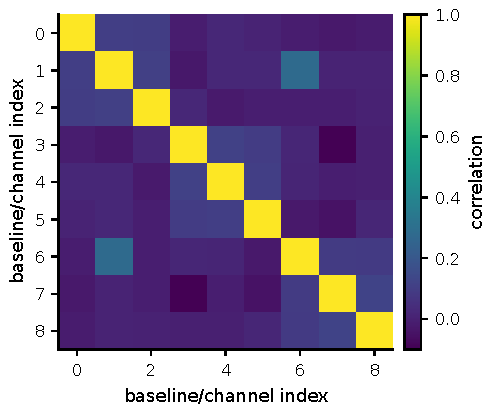
\includegraphics[width=0.66\linewidth]{figures/generated/chapter_07/ch07_covariance_matrix.pdf}
\caption{A schematic covariance matrix of multi-baseline/multi-channel results. The diagonal is the single-point variance, the blocks near the diagonal come from noise shared by the same time period or the same telescope, and the structure far from the diagonal may come from a common background estimate, zero-baseline normalization, or electronic crosstalk. If a fit uses only diagonal errors, it overestimates the "effective amount of independent information" and the error bars become spuriously small.}
\label{fig:e14-cov}
\end{figure}

One final piece of advice: all null tests must use the \textbf{same} selection function and weights as the main analysis. Common null tests include: shifting one stream to a nonphysical delay, swapping the sign of the geometric delay, using two polarization or wavelength channels that should not be correlated, using off-target sky as background, splitting the telescope pair into different time blocks, removing a certain telescope or night one at a time, and injecting a known correlation peak into the real event table to see whether it can be recovered without bias. If the main signal only appears below some threshold, and vanishes upon moving the threshold, using a wrong delay, or doing a jackknife, then it is more likely a product of pipeline selection or instrument state than a celestial correlation.

\section{White noise settles, systematic error is the ceiling}
\label{sec:e14-floor}

Chapter~\ref{chap:e12} used Fisher information to answer "how much information is really in the data." Here we connect it to time, and make clear the most critical watershed in an observation plan: white noise and systematic error have completely different fates.

\textbf{White noise (statistical noise) settles.} It comes from the Poisson fluctuation of photons and the random noise of electronics, one independent sample after another. The conclusion of Chapter~\ref{chap:e03}: the more independent samples, the more stable the mean, and the error falls with the effective photon number $N_{\rm eff}$ as $N_{\rm eff}^{-1/2}$, that is, with integration time as $T^{-1/2}$. In Fisher language, the information of independent data points \textbf{adds}, the total information grows linearly with $N_{\rm eff}$, and the parameter error given by the Cramér--Rao bound shrinks inversely as the square root of the information: as long as you are willing to integrate, it keeps falling.

\textbf{Systematic error (systematic bias) does not settle.} It comes from \textbf{consistent offsets} such as inaccurate calibration, imperfectly subtracted background, gain drift, a nonzero zero baseline, and biased electronic- or optical-bandwidth calibration. They are not independent samples each time, but push each data point the same little bit in the same direction. Integrate ten times longer and the white noise drops to $1/\sqrt{10}$, but this offset does not budge: it becomes a horizontal \textbf{floor}, and the error can go no lower.

Why is this floor especially deadly for us? Because the intensity-interferometry signal is inherently only as faint as $10^{-6}$--$10^{-4}$ (recall the example below Eq.~\eqref{eq:e14-accidental} of the $3.6\times10^4$-pair excess pressed on a $3.6\times10^8$ background). When the excess you want to measure is only one part in a million, then a consistent bias of just a few parts in a million in the background calibration is enough to be of the same order as the signal, or even to drown it. In other words: the faint signal presses the tolerance for systematic error down to the same demanding $10^{-6}$ level, and this is precisely the root of the field's dictum that "systematic terms are the ceiling."

To make this sentence mathematical, feed the covariance of Eq.~\eqref{eq:e14-cov} into the Fisher matrix (derivation in Chapter~\ref{chap:e12}):
\begin{equation}
  F_{\alpha\beta}
  =\frac{\partial\bm m^{T}}{\partial\theta_\alpha}\,\Sigma^{-1}\,\frac{\partial\bm m}{\partial\theta_\beta},
  \qquad
  \operatorname{Cov}(\theta_\alpha,\theta_\beta)\gtrsim(F^{-1})_{\alpha\beta} .
  \label{eq:e14-fisher}
\end{equation}
\begin{formulaexplain}
$F_{\alpha\beta}$ is the Fisher information matrix: $\partial\bm m/\partial\theta$ is the sensitivity of the model to the parameter, and $\Sigma^{-1}$ weights by the covariance. Its inverse $F^{-1}$ approximately gives the lower bound on the parameter covariance. It is the workhorse tool for observation planning and high-signal-to-noise error estimation.
\end{formulaexplain}
From this formula two scalings can be read at a glance. First, the \textbf{scaling with photon number}: if $\Sigma$ is dominated by independent photon statistics, then $\Sigma^{-1}\propto N_{\rm eff}$, $F\propto N_{\rm eff}$, and the parameter error $\propto N_{\rm eff}^{-1/2}$: this is the settling of white noise. Second, the \textbf{scaling with baseline}: the Fisher information is additive over mutually independent $uv$ points, $F=\sum_{\text{baselines}}$ (one term per baseline), so adding one more baseline adds one more piece of information. But whether a baseline is worth it depends on whether it falls where the model $|V|^2$ is most sensitive to the parameter, i.e. where $\partial\bm m/\partial\theta$ is largest: for measuring an angular diameter, the most valuable baseline falls near the first zero of the visibility curve (see the $uv$-coverage discussion of Chapters~\ref{chap:e10} and~\ref{chap:e11}), whereas a short baseline where $|V|^2\approx1$ carries almost no angular-diameter information. But once a systematic floor that does not fall with time appears in $\Sigma$, $\Sigma^{-1}$ saturates, and no matter how many more photons or how much longer the integration, $F$ no longer grows: the error tends to the floor and stops.

\begin{figure}[tbp]
\centering
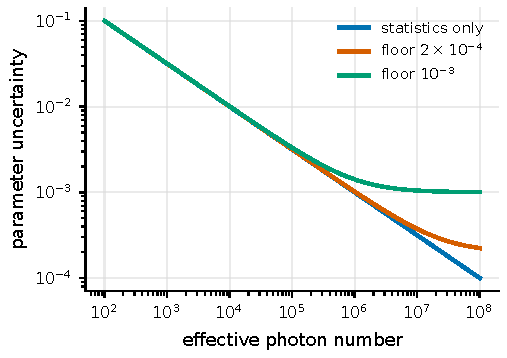
\includegraphics[width=0.70\linewidth]{figures/generated/chapter_07/ch07_fisher_scaling.pdf}
\caption{The scaling of parameter error with the effective photon number. The blue curve is the pure-statistical $N_{\rm eff}^{-1/2}$ settling; the orange and green curves, after adding systematic floors of different heights, no longer improve the final error at long integration. An observation plan must put integration time, target brightness, baseline coverage, and systematic calibration into the same error budget, which is precisely the theme of Chapter~\ref{chap:e15}.}
\label{fig:e14-fisher}
\end{figure}

A final reminder: the Fisher matrix is a local quadratic approximation near the likelihood peak, reliable only at high signal-to-noise and when the posterior is near-Gaussian. For a multi-peaked posterior, a nonlinear degeneracy, or a parameter near a boundary, one must switch to MCMC or nested sampling \citep{1925PCPS...22..700F,2013PASP..125..306F,2009MNRAS.398.1601F}.

\section{From correlation products to physical parameters}
\label{sec:e14-fit}

With the correlation products and their covariance in hand, the last step is to fit out the physical parameters. First write the \textbf{model vector}: map the angular diameter, binary separation, brightness ratio, ring radius, or jet parameters into the squared visibility at each $uv$ point and each wavelength:
\begin{equation}
  \bm m(\bm\theta)
  =\Big[\,|V(\bm u_1,\lambda_1\mid\bm\theta)|^2,\ \ldots,\ |V(\bm u_{N_d},\lambda_{N_d}\mid\bm\theta)|^2\,\Big] .
  \label{eq:e14-model}
\end{equation}
\begin{formulaexplain}
$\bm m(\bm\theta)$ is the data vector predicted by the physical model, each entry being the $|V|^2$ at spatial frequency $\bm u_i$ and wavelength $\lambda_i$. It translates the angular-diameter, binary, and structure parameters into observables directly comparable with $\bm d$.
\end{formulaexplain}
Here $\bm u=\bm B_\perp/\lambda$ is the spatial frequency (the projected baseline in units of wavelength, see the van Cittert--Zernike theorem of Chapter~\ref{chap:e10}). If the data vector $\bm d$ is already approximately Gaussian, the likelihood is the covariance-weighted residual:
\begin{equation}
  -2\ln L
  =\big[\bm d-\bm m(\bm\theta)\big]^{T}\Sigma^{-1}\big[\bm d-\bm m(\bm\theta)\big]
   +\ln|\Sigma|+\text{const} .
  \label{eq:e14-gauss}
\end{equation}
\begin{formulaexplain}
$\bm d-\bm m$ is the data-minus-model residual, $\Sigma^{-1}$ weights by the covariance (correlated points do not count information twice), and $\ln|\Sigma|$ is the normalization term. This is the most common Gaussian likelihood for data products with correlated errors, and minimizing it gives the optimal parameters.
\end{formulaexplain}
Note that the $\Sigma^{-1}$ step is precisely the payoff of Section~\ref{sec:e14-cov}: using the full covariance rather than diagonal errors is what prevents treating correlated points as mutually independent and overcounting the information. If you fit the raw low-count delay cells directly, do not use the Gaussian; return to the Poisson likelihood of Eq.~\eqref{eq:e14-binned-poisson}. VERITAS-SII fits the variation of $|g^{(1)}|^2$ with projected baseline using uniform-disk and limb-darkening models; MAGIC-SII converts the Pearson correlation into $|V|^2$ through flux and background calibration and then fits the angular diameter and systematic error \citep{2020NatAs...4.1164A,2024MNRAS.529.4387A,1967MNRAS.137..375H}.

When the posterior may be multi-peaked, or external priors are needed, write it as a \textbf{Bayesian posterior}:
\begin{equation}
  p(\bm\theta\mid\mathcal D,M)=\frac{L(\mathcal D\mid\bm\theta,M)\,\pi(\bm\theta\mid M)}{Z_M},
  \qquad
  Z_M=\int L\,\pi\,d\bm\theta .
  \label{eq:e14-posterior}
\end{equation}
\begin{formulaexplain}
$p(\bm\theta\mid\mathcal D,M)$ is the parameter posterior under model $M$, $L$ is the likelihood, $\pi$ is the prior, and $Z_M$ is the model evidence (the normalization constant, also used to compare models). It combines the data constraint and external physical knowledge into a complete uncertainty.
\end{formulaexplain}
The prior $\pi$ can hold the distance, spectral type, known angular diameter, binary orbit, burst time, or physical boundaries, and it must be stated clearly, because intensity interferometry often measures only $|V|^2$ and lacks the phase, causing mirror, brightness-ratio, and position-angle degeneracies, and it is the prior that helps hold the degeneracy down. As for sampling, emcee suits moderate-dimensional posteriors, and MultiNest suits multi-peaked posteriors and evidence estimation \citep{2013PASP..125..306F,2009MNRAS.398.1601F}; but the sampler cannot replace physical checks: the chain's autocorrelation time, acceptance rate, prior volume, and "whether an injected known signal can be recovered without bias" must all be reported together \citep{1992ApJ...398..146G}. Only then is the chain from event table to error-bearing parameters closed; Chapter~\ref{chap:e15} will put it into the complete observation design and feasibility assessment.

\section{Chapter Summary}
\label{sec:e14-summary}

\begin{itemize}
  \item \textbf{Build the model first, then compute the estimator.} The event table must first be written as a selection function Eq.~\eqref{eq:e14-selection} and a Poisson likelihood Eq.~\eqref{eq:e14-point-likelihood}/\eqref{eq:e14-binned-poisson}; the point-process likelihood arises naturally from "taking the limit of infinitely narrow bins," and preserves the time information lost after binning.
  \item \textbf{The correlation peak is a faint excess on a huge background.} The delay histogram Eq.~\eqref{eq:e14-paircount} only becomes meaningful after dividing by the accidental-coincidence background Eq.~\eqref{eq:e14-accidental}; the true signal is only $10^{-6}$--$10^{-4}$ of the background, which fundamentally determines the requirements on integration time and calibration precision.
  \item \textbf{Finishing the computation relies on algorithms, not brute force.} Pair-by-pair $N^2$/$N(N-1)/2$ is fit only for teaching; the sorted window Eq.~\eqref{eq:e14-window} is nearly linear, and the FFT (XF/FX) scales as $N_{\rm bin}\log N_{\rm bin}$; with few stations the bottleneck is the number of time samples each pair swallows, and GPU/FPGA real-time, dead-time-free correlation computes the whole stretch of fluctuation.
  \item \textbf{The error is not independent error bars.} Shared telescope, background, and calibration make off-diagonal terms appear in the covariance Eq.~\eqref{eq:e14-cov}; estimate $\Sigma$ with time-block bootstrap/jackknife/injection simulation, and the fit Eq.~\eqref{eq:e14-gauss} must use the full $\Sigma^{-1}$.
  \item \textbf{White noise settles, systematic error is the ceiling.} The statistical error falls with $N_{\rm eff}^{-1/2}$, $T^{-1/2}$, and the Fisher information grows linearly with photon number and adds over independent baselines; but a consistent offset forms a floor that does not fall with integration, and the faint signal presses the systematic tolerance down to the same demanding order.
\end{itemize}

\medskip
\noindent\textbf{Questions to Ponder.}
(1) If the delay cell width $\Delta\tau$ is halved, how do the accidental-coincidence background $B_{ab,k}$ and the signal excess each change, and does the final signal-to-noise ratio improve?
(2) You have 4 telescopes; why does "only 6 pairs" not mean the correlator is easy? On which quantity is the bottleneck?
(3) A team increased its integration time tenfold, but the error bars barely shrank. In this chapter's language, what is the most likely diagnosis? Which null tests should be done to confirm it?

\chapter{Observation Design, Error Budget, and Feasibility}
\label{chap:e15}

\begin{chapteropening}
Up to this point, we have assembled the full toolbox: Chapter~\ref{chap:e11} told us how the signal-to-noise ratio of intensity interferometry scales with telescope area, photon rate, and integration time; Chapter~\ref{chap:e12} told us how much extractable information is really hidden in a dataset (Fisher information and the Cramér--Rao lower bound); Chapter~\ref{chap:e13} explained detectors, clocks, and event tables, and Chapter~\ref{chap:e14} explained how the correlator turns an event table into $g^{(2)}(\tau)$ and $|V|^2(B)$. What we must do now is \textbf{assemble these parts into one real observation}. Imagine before you a blank observing proposal form: which star will you observe? With how many telescopes, how long a baseline, how wide a filter? For how long will you expose? And in the end, to what fraction of a percent can you measure the angular diameter? This chapter is the process of filling in this form from beginning to end. At its core is a \textbf{ledger}: the photon rate gives the statistical ceiling, the correlation contrast gives the target signal, and the baseline, bandwidth, time resolution, and calibration error decide whether this signal can survive out of the noise. We will compute every step as a real number, and finally walk through a complete feasibility calculation, from one real bright star to an achievable precision.
\end{chapteropening}

\section{An observation is a ledger from parameters to data}
\label{sec:e15-ledger}

Every observation, at bottom, is for the sake of estimating a few physical numbers. The angular diameter of a star, the angular separation of a binary, the oblateness and long-axis direction of a rapid rotator, the radius of a spectral-line emitting region, the rotation of the polarization angle, the time delay between two signal paths, the height of a second-order correlation peak: these are what we really want, called the \textbf{physical parameters}, denoted $\bm\theta_{\rm phys}$. But what the instrument hands us is never these numbers; it is the \textbf{event list} of Chapter~\ref{chap:e13}: one photon per line, carrying arrival time, telescope number, wavelength, and polarization labels. The physical parameters must be \emph{inferred backwards} from these fields.

So the first thing in designing an observation is not to ask "which star do I want to look at," but to ask "do the numbers I want have supporting fields in the event table?" To do nanosecond-scale time correlation, the time-stamp precision must be compressed to the nanosecond; to give the required baseline, the position labels must be recorded accurately; to separate bands or measure polarization, the wavelength and polarization labels must not be erased at the moment of recording. Here is a principle easily overlooked yet fatal: \textbf{once information is averaged away at the recording stage, it can never be recovered afterwards}. If you store only one long-integration image from the start, then nanosecond time correlation and polarization correlation have already vanished with the averaging; whereas if you honestly store the entire event table, you can afterwards project it arbitrarily into a light curve, $g^{(2)}(\tau)$, $|V|^2(B)$, polarization angle, or multi-wavelength $u,v$ data. The event table is the "raw broth," and the image is only "one spoonful after boiling it dry."

The whole chain from parameters to data can be written as a likelihood:

\begin{equation}
  \mathcal L(\bm\theta_{\rm phys})
  =
  P\!\left(\,d \;\middle|\;
  q_{\rm inst}(\bm\theta_{\rm phys}),\;
  \bm c_{\rm cal},\;
  \bm b_{\rm sky}
  \right).
  \label{eq:e15-likelihood}
\end{equation}
\begin{formulaexplain}
$\bm\theta_{\rm phys}$: the physical parameters to be estimated (such as the angular diameter $\theta$). $d$: the observed data or its statistic. $q_{\rm inst}$: the quantity the instrument actually measures (such as $|V|^2$). $\bm c_{\rm cal}$: the calibration parameters. $\bm b_{\rm sky}$: the sky background. This formula says: the physical parameters are first "translated" by the instrument into observables, and then, together with calibration and background, determine the probability of the data appearing.
\end{formulaexplain}

Let us land each symbol. $\mathcal L$ is the likelihood, dimensionless, measuring "if the true parameters are $\bm\theta_{\rm phys}$, how probable is it to see this data $d$." $q_{\rm inst}$ is the instrument observable: it can be the squared visibility $|V|^2$ (dimensionless), the excess of the second-order correlation $g^{(2)}-1$ (dimensionless), a polarization Stokes component, or an arrival-time residual (seconds). $\bm c_{\rm cal}$ are the calibration parameters (time zero point, filter passband, detector efficiency, gain state), which are not the physical quantities we want, yet contaminate the data and must be estimated jointly or measured in advance. $\bm b_{\rm sky}$ is the skyglow, moonlight, dark counts, and host-galaxy background. When writing an observing proposal, rather than vaguely saying "we will observe this star," what is truly useful is to compute this chain all the way through: what is this star's magnitude $m_B$, how large is its estimated angular diameter $\theta$, how long is its visibility window, which $|V|^2$ data points the model prior gives, and to what fraction of a percent the error of $\theta$ can finally be pressed. The remaining sections of this chapter fill in this chain, segment by segment, with real numbers.

\section{Photon budget: from magnitude to effective photon number}
\label{sec:e15-photon-budget}

Everything begins with the photon rate. No matter how interesting a star is, if it gives you only a few photons per second, any correlation signal will drown in the noise. So the first step of a feasibility calculation is always to \textbf{translate the magnitude into photons per second}. This translation has four steps: magnitude $\to$ spectral flux density $\to$ photon flux per unit area $\to$ multiply by area and efficiency to get the effective photon rate. Let us take them one by one.

\paragraph{Step 1: magnitude to spectral flux density}

Astronomy uses the magnitude to describe brightness, with each 5 magnitudes smaller being 100 times brighter: this is a logarithmic ruler. The advantage of the AB magnitude is that it corresponds directly to the spectral flux density:

\begin{equation}
  F_\nu = 3631\,{\rm Jy}\times 10^{-0.4\,m_{\rm AB}}.
  \label{eq:e15-ab-flux}
\end{equation}
\begin{formulaexplain}
$m_{\rm AB}$: the AB magnitude (dimensionless). $F_\nu$: the spectral flux density per unit frequency. $1\,{\rm Jy}=10^{-23}\,{\rm erg\,s^{-1}\,cm^{-2}\,Hz^{-1}}$. The constant $3631\,{\rm Jy}$ is the defining flux of $m_{\rm AB}=0$. Each increase of 5 in magnitude drops $F_\nu$ by a factor of 100.
\end{formulaexplain}

Here $F_\nu$ is the spectral flux density, with dimensions of "energy / (time $\cdot$ area $\cdot$ frequency)," in CGS units ${\rm erg\,s^{-1}\,cm^{-2}\,Hz^{-1}}$; $1\,{\rm Jy}$ (jansky) $=10^{-23}$ of this unit. Take a star of $m_{\rm AB}=5$, and substituting gives
\[
  F_\nu = 3631\,{\rm Jy}\times 10^{-0.4\times5}
        = 3631\times10^{-2}\,{\rm Jy}
        = 36.3\,{\rm Jy}
        = 3.63\times10^{-22}\,{\rm erg\,s^{-1}\,cm^{-2}\,Hz^{-1}} .
\]
This is the energy this star delivers each second across each square centimetre, at each hertz of frequency. The number is very small: one square centimetre, one hertz of bandwidth, receives only $10^{-22}$ erg in one second, which reminds us that we must later gather it up with large area and wide bandwidth.

\paragraph{Step 2: energy flux to photon flux}

The detector counts not energy but numbers of photons. A photon of frequency $\nu$ carries energy $h\nu$ ($h=6.63\times10^{-27}\,{\rm erg\,s}$ is Planck's constant). Dividing the energy flux by the single-photon energy gives the number of photons per unit area, per unit time, per unit bandwidth. Multiplying by the optical bandwidth $\Delta\nu$ gives the number of photons per square centimetre per second over the whole passband. The bandwidth conversion follows the relation of Chapter~\ref{chap:e02}, $\Delta\nu\simeq c\,\Delta\lambda/\lambda^2$. Take the observing wavelength $\lambda=550\,{\rm nm}$ and passband $\Delta\lambda=10\,{\rm nm}$:
\[
  \nu=\frac{c}{\lambda}=\frac{3\times10^{10}\,{\rm cm\,s^{-1}}}{550\times10^{-7}\,{\rm cm}}
     =5.45\times10^{14}\,{\rm Hz},
  \qquad
  h\nu = 6.63\times10^{-27}\times5.45\times10^{14}
       = 3.61\times10^{-12}\,{\rm erg},
\]
\[
  \Delta\nu = \frac{c\,\Delta\lambda}{\lambda^2}
            = \frac{3\times10^{10}\times10\times10^{-7}}{(550\times10^{-7})^2}
            = 9.9\times10^{12}\,{\rm Hz}\approx10^{13}\,{\rm Hz}.
\]
Hence the photon flux per unit area
\[
  \Phi = \frac{F_\nu\,\Delta\nu}{h\nu}
       = \frac{3.63\times10^{-22}\times 9.9\times10^{12}}{3.61\times10^{-12}}
       \approx 1.0\times10^{3}\ {\rm photons\,s^{-1}\,cm^{-2}} .
\]
One square centimetre, a 10 nm passband, about a thousand photons per second: this is the raw flux \emph{arriving at the top of the atmosphere}, not yet discounted.

\paragraph{Step 3: multiply by area and efficiency to get the effective photon rate}

The photons that truly fall into the correlator must be multiplied by two more factors: the telescope's \textbf{effective collecting area} $A$, and the \textbf{total efficiency} $\eta$ from the atmosphere to photon counting. The latter folds atmospheric transmission, mirror reflectivity, filter transmission, fibre-coupling loss, and detector quantum efficiency (see Chapter~\ref{chap:e07}) all into one number, with a typical value $\eta\sim0.2$--$0.3$. Together:

\begin{equation}
  R_\gamma
  = \eta\,A\,\frac{F_\nu\,\Delta\nu}{h\nu}
  = \eta\,A\,\Phi .
  \label{eq:e15-photon-rate}
\end{equation}
\begin{formulaexplain}
$R_\gamma$: the effective photon rate (counts per second). $\eta$: the total efficiency (dimensionless, including atmosphere, mirror, filter, detector). $A$: the effective collecting area (${\rm cm^2}$). $\Phi$: the photon flux per unit area. This formula finally turns "how bright the star is" into "how many times the detector fires per second."
\end{formulaexplain}

Plug in real numbers. An imaging atmospheric Cherenkov telescope (IACT) of 12 m aperture has a collecting area $A=\pi(6\,{\rm m})^2\approx113\,{\rm m^2}=1.13\times10^6\,{\rm cm^2}$. Take $\eta=0.25$, $m_{\rm AB}=5$:
\[
  R_\gamma = 0.25\times1.13\times10^6\times1.0\times10^3
          \approx 2.8\times10^8\ {\rm s^{-1}} .
\]
About three hundred million photons per second. If this star is as faint as $m_{\rm AB}=8$ (3 magnitudes fainter than 5, flux down by a factor of $10^{-1.2}=0.063$), then $R_\gamma\simeq1.8\times10^7\,{\rm s^{-1}}$. For a 17 m-class aperture (such as MAGIC), the area is 2 times larger, and the two cases are about $5.7\times10^8$ and $3.6\times10^7\,{\rm s^{-1}}$ respectively. Large as these numbers are, they are \emph{not yet the usable correlation event rate}: they will subsequently be whittled down, layer by layer, by the number of spatial modes, polarization, oblique filter incidence, detector dead time, data-quality slicing, and background correction \citep{2006ApJ...649..399L,2020MNRAS.491.1540A,2021MNRAS.506.1585Z,2024MNRAS.529.4387A}. Figure~\ref{fig:e15-photon-rate} plots this magnitude-to-photon-rate curve.

\begin{figure}[tbp]
\centering
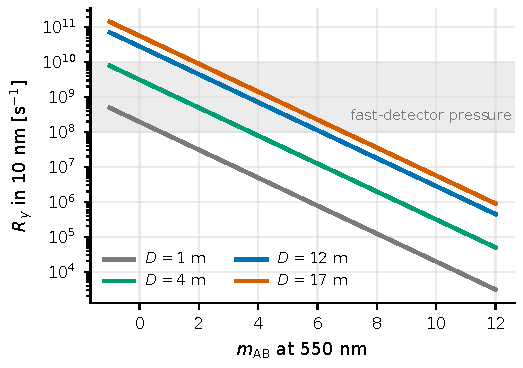
\includegraphics[width=0.86\linewidth]{figures/generated/chapter_18/ch18_photon_rate_magnitude.pdf}
\caption{The conversion from AB magnitude to narrowband photon rate. The curve uses a 550 nm, 10 nm passband and total efficiency $\eta=0.25$. Aperture changes the collecting area only linearly, and each increase of 5 magnitudes drops the photon rate by a factor of 100; the grey region marks the range above $10^8\,{\rm s^{-1}}$, where pressure on high-speed detection and data throughput begins.}
\label{fig:e15-photon-rate}
\end{figure}

\paragraph{Coherence dilution: why the raw photon rate is not the usable signal}

What intensity interferometry truly wants to measure is that tiny bump of the second-order correlation at zero delay, whose height is jointly determined by the optical \textbf{coherence time} $\tau_c$ (Chapter~\ref{chap:e02}) and the electronic response time. The coherence time is "the time the light wave still remembers its own phase," set by the bandwidth: $\tau_c\simeq1/\Delta\nu\simeq\lambda^2/(c\,\Delta\lambda)$. Take the 416 nm, 13 nm passband commonly used by VERITAS:
\[
  \tau_c\simeq\frac{\lambda^2}{c\,\Delta\lambda}
  =\frac{(416\times10^{-7})^2}{3\times10^{10}\times13\times10^{-7}}
  \approx 4.4\times10^{-14}\,{\rm s} .
\]
This is tens of femtoseconds, far faster than any electronics. The equivalent time width of the detector plus electronic chain is $\Delta t\sim4\,{\rm ns}$. The true correlation peak holds only within this narrow time $\tau_c$, yet it is flattened out across the wide time bin $\Delta t$, so the peak height is diluted by about $\tau_c/\Delta t$:
\[
  \frac{\tau_c}{\Delta t}\approx\frac{4.4\times10^{-14}}{4\times10^{-9}}
  \approx1.1\times10^{-5}.
\]
So the normalized correlation peak of unresolved thermal light at zero baseline naturally falls to the order of a few $10^{-6}$: this is precisely the $N_0\sim10^{-6}$ tier measured in the VERITAS papers \citep{2020NatAs...4.1164A,2024ApJ...966...28A}. That the peak is so low means it can only "surface" from the noise by long-time averaging and strict calibration. Figure~\ref{fig:e15-coherence} plots this dilution.

\begin{figure}[tbp]
\centering
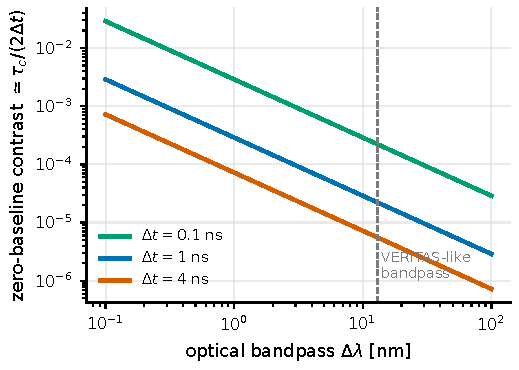
\includegraphics[width=0.86\linewidth]{figures/generated/chapter_18/ch18_coherence_dilution.pdf}
\caption{The wider the passband, the shorter the optical coherence time; the slower the electronic time resolution, the more the zero-delay correlation peak is diluted. The combination of 416 nm, 13 nm, 4 ns gives a contrast of a few $10^{-6}$, so the correlation peak can only appear from the noise by long integration and strict calibration.}
\label{fig:e15-coherence}
\end{figure}

Here lies a counterintuitive but extremely important fact: \textbf{widening the optical passband does not improve the signal-to-noise ratio proportionally}. A wide band does bring more photons ($R_\gamma\propto\Delta\lambda$), but at the same time shortens the coherence time and lowers the correlation contrast in each time bin ($\propto\tau_c\propto1/\Delta\lambda$). The two nearly cancel exactly in the signal-to-noise ratio; the next section will make this evident. A real instrument still has to choose a filter, but that is to control the PMT current, sky background, oblique-incidence effect, or to select spectral lines, not simply "the wider the better" \citep{2020MNRAS.491.1540A,2024MNRAS.529.4387A}.

\section{How to estimate signal-to-noise ratio and integration time}
\label{sec:e15-snr}

With the photon rate, we can ask the question we care about most: how long must one expose for the signal to be strong enough? The intensity-interferometry signal-to-noise scaling derived in Chapter~\ref{chap:e11} is the core of all this:

\begin{equation}
  {\rm SNR}
  = A\,\alpha\,n\,|V(\bm B)|^2\,
    \sqrt{\frac{\Delta f\,T}{2}} .
  \label{eq:e15-snr}
\end{equation}
\begin{formulaexplain}
$A$: the collecting area (${\rm cm^2}$). $\alpha$: the quantum efficiency (dimensionless). $n$: the incident spectral photon density ${\rm photons\,s^{-1}\,cm^{-2}\,Hz^{-1}}$. $|V|^2$: the squared visibility. $\Delta f$: the electronic bandwidth (Hz). $T$: the integration time (s). The signal accumulates as $\sqrt{T}$.
\end{formulaexplain}

First nail down each symbol. $A$ is the effective area of each telescope (${\rm cm^2}$); $\alpha$ is the quantum efficiency (dimensionless); $n$ is the \textbf{incident spectral photon density}, the number of photons per unit area, per unit time, per unit optical bandwidth, with dimensions ${\rm photons\,s^{-1}\,cm^{-2}\,Hz^{-1}}$, determined by the source's surface brightness (i.e. brightness temperature), \emph{independent of how wide an optical passband you choose}. $|V(\bm B)|^2$ is the squared visibility on baseline $\bm B$ (dimensionless, between 0 and 1), the target signal we truly want to measure. $\Delta f$ is the electronic bandwidth (Hz), the equivalent bandwidth jointly determined by the light pulse, PMT/SPAD response, cabling, amplifier, digitizer, and software correlation. $T$ is the integration time (s).

This formula has several things worth chewing over. First, look at $A\,\alpha\,n$ combined: its dimensions are ${\rm s^{-1}\,Hz^{-1}}$, and since ${\rm Hz^{-1}=s}$, the whole is \emph{dimensionless}: it is the mean photon occupation number per mode $\delta=A\alpha n$, i.e. the \textbf{photon degeneracy}. Visible-light thermal stars have $\delta$ of only $10^{-4}$--$10^{-2}$, which is precisely the root of why the intensity-interferometry signal is so faint. Second, because $n$ is a \emph{spectral} density, widening the optical passband does not change $n$: this confirms from the formula the sentence of the previous section, "a wide band does not earn signal-to-noise for free." Third, and most practical: ${\rm SNR}\propto\sqrt{T}$. The signal accumulates not linearly but by the \emph{square root}: to double the signal-to-noise ratio, one must expose for four times as long. This $\sqrt{T}$ law will become the protagonist of the error budget in the next section.

Plug in a real scenario. LeBohec and Holder take $A=100\,{\rm m^2}$, $\alpha=0.3$, $\Delta f=1\,{\rm GHz}$, $T=5\,{\rm h}=1.8\times10^4\,{\rm s}$, $|V|^2=0.5$, and compute that a star of $m_V\simeq6.7$ falls just at the $5\sigma$ tier; under the same conditions a star of $m_V=5$ (1.7 magnitudes brighter, $n$ about 5 times larger) has a signal-to-noise ratio soaring past twenty, while a star of $m_V=9$ has less than $1\sigma$ left, i.e. is unmeasurable \citep{2006ApJ...649..399L,2008AIPC..984..205L}. Plotting this dependence as a magnitude--integration-time heatmap gives Figure~\ref{fig:e15-snr}. Solving conversely for the integration time is also direct: solve Eq.~\eqref{eq:e15-snr} for $T$,
\[
  T = \frac{2\,{\rm SNR}^2}{(A\alpha n)^2\,|V|^4\,\Delta f},
\]
that is, the required time grows with the \emph{square} of the target signal-to-noise ratio, and falls \emph{inversely} with the square of the degeneracy and the fourth power of the visibility, which explains why a fainter target, or one already highly resolved ($|V|^2$ very small), makes the integration time rapidly run out of control.

\begin{figure}[tbp]
\centering
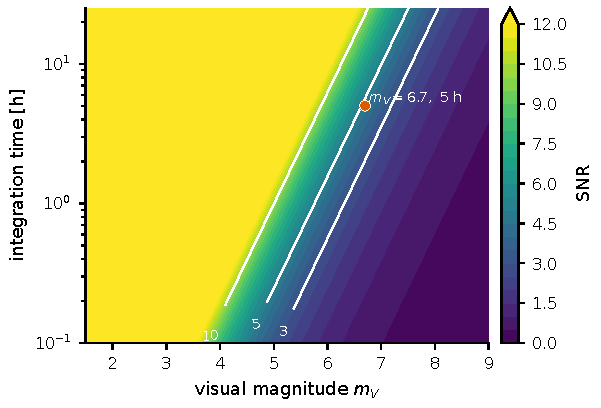
\includegraphics[width=0.90\linewidth]{figures/generated/chapter_18/ch18_snr_heatmap.pdf}
\caption{The dependence of the intensity-interferometry signal-to-noise ratio on magnitude and integration time. The figure takes $A=100\,{\rm m^2}$, $\alpha=0.3$, $\Delta f=1\,{\rm GHz}$, $|V|^2=0.5$; the orange point corresponds to the $m_V\simeq6.7$, 5 h $\approx5\sigma$ position in the LeBohec--Holder estimate.}
\label{fig:e15-snr}
\end{figure}

When using Eq.~\eqref{eq:e15-snr} for a first-round estimate, remember it is the "ideal version." In real data, $T$ is the effective exposure time (live time) after quality slicing, not wall-clock time; $\Delta f$ is the equivalent bandwidth of the whole electronic chain; and $|V|^2$ also varies slowly with the target's altitude and hour angle. Take a set of real engineering numbers: VERITAS uses four 12 m telescopes to give six baselines simultaneously, with a 416 nm, about 13 nm filter and 4 ns sampling, spitting out about 3.5 TB of raw data per hour; MAGIC uses two 17 m telescopes and a central PMT, and its early demonstration reported a sensitivity about an order of magnitude higher than Narrabri. The Vega photon-counting experiment took another route: using a single-photon avalanche diode (SPAD) plus software correlation, it measured $\langle g^{(2)}\rangle=1.0034\pm0.0008$ at zero baseline, while at a projected baseline of about 2 km it showed \emph{no} correlation, exactly as expected since Vega's angular diameter of about 3.3 mas is already fully resolved on that baseline \citep{2020NatAs...4.1164A,2020MNRAS.491.1540A,2021MNRAS.506.1585Z}.

Multiple telescopes buy two things at once: more data and more geometry. $N$ telescopes give $N(N-1)/2$ simultaneous baselines: 4 give only 6, but 60 give 1770. The key is that different baselines sample the source structure at \emph{different points} in the $u,v$ plane, and are by no means repeated measurements of the same number (Chapter~\ref{chap:e11}). To measure the diameter of a uniform disk, a few suitable baselines suffice; but to measure the oblateness of a rapid rotator, a binary, a disk wind, or a non-axisymmetric spectral-line emitting region, position-angle coverage is indispensable. For covering hot-star structures of 0.1--3 mas, the whole baseline range of 30--2000 m is more useful than simply piling up one longest baseline. Figure~\ref{fig:e15-uv} compares the $u,v$ coverage of a small array and a large array.

\begin{figure}[tbp]
\centering
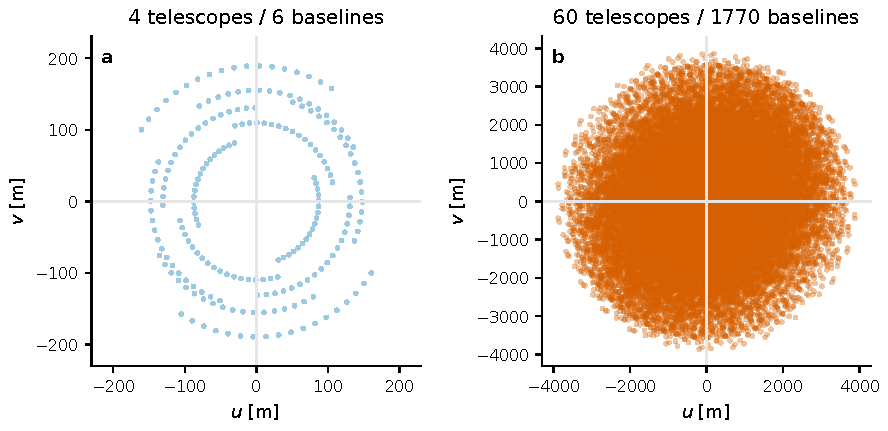
\includegraphics[width=0.94\linewidth]{figures/generated/chapter_18/ch18_uv_coverage.pdf}
\caption{How array size changes $u,v$ sampling. Left: the six baselines of four telescopes, still relatively sparse after rotation with hour angle; right: a multi-telescope array with short, medium, and long baselines present at once. Dense coverage does not automatically mean high signal-to-noise, but it decides whether a non-axisymmetric target can be stably fit or reconstructed.}
\label{fig:e15-uv}
\end{figure}

\section{Baseline, bandwidth, and band choice are decided by the visibility slope}
\label{sec:e15-baseline}

With the signal-to-noise ratio in hand, why can we still not fix the baseline right away? Because \textbf{strong signal} and \textbf{much information} are two different things. A baseline may have a very high correlation peak (very good signal-to-noise), yet be almost insensitive to the angular diameter we want to measure, and then no matter how precisely it measures, it is useless. To judge "which baseline actually carries diameter information," one must look at the \emph{slope} of the visibility curve.

First set out the rough relation between angular scale and baseline. To resolve an angular scale $\theta$, the required baseline is about

\begin{equation}
  B\sim\frac{\lambda}{\theta}
  = 86\,{\rm m}\left(\frac{\lambda}{416\,{\rm nm}}\right)
                \left(\frac{1\,{\rm mas}}{\theta}\right).
  \label{eq:e15-baseline}
\end{equation}
\begin{formulaexplain}
$B$: the required baseline (m). $\lambda$: the observing wavelength. $\theta$: the target angular scale (here in mas). This is an order-of-magnitude formula: to resolve a smaller angle, a longer baseline is needed; the shorter the wavelength, the finer the same baseline resolves.
\end{formulaexplain}

Plug in a few numbers for a picture: a $\theta=2\,{\rm mas}$ hot star at 416 nm begins to be resolved at only about 43 m; $\theta=0.5\,{\rm mas}$ needs about 170 m; $\theta=0.1\,{\rm mas}$ requires reaching about 860 m. Narrabri's maximum baseline is about 188 m, so it is best at bright, hot stars with angular diameters from a few tenths to a few mas; a CTA-class kilometre array can push the spatial frequency to tens of microarcseconds, but the target must still have enough photon rate to afford it \citep{1974MNRAS.167..121H,2006ApJ...649..399L}.

Now look at the slope. The squared visibility of a uniform disk (Chapter~\ref{chap:e11}) is first a plateau near 1 with baseline, then decreases, hitting bottom at the first zero. The crux of observation design is: if all your baselines fall on the $|V|^2\simeq1$ plateau, the curves for different $\theta$ nearly coincide and you cannot tell the star's size at all; if you only measure the extremely low visibility \emph{after} the first zero, the correlation peak is so low it hugs the noise. \textbf{Diameter information is concentrated on the section of the baseline where the curve drops most steeply, i.e. where the slope $|\partial|V|^2/\partial\theta|$ is largest}, usually in the descending region of the first lobe and near the first zero. So a serious feasibility calculation must not only plot the target model's $|V|^2(B)$, but also its derivative with respect to the parameter, $\partial|V|^2/\partial\theta$, to see which baseline the peak falls on (Figure~\ref{fig:e15-vis}).

\begin{figure}[tbp]
\centering
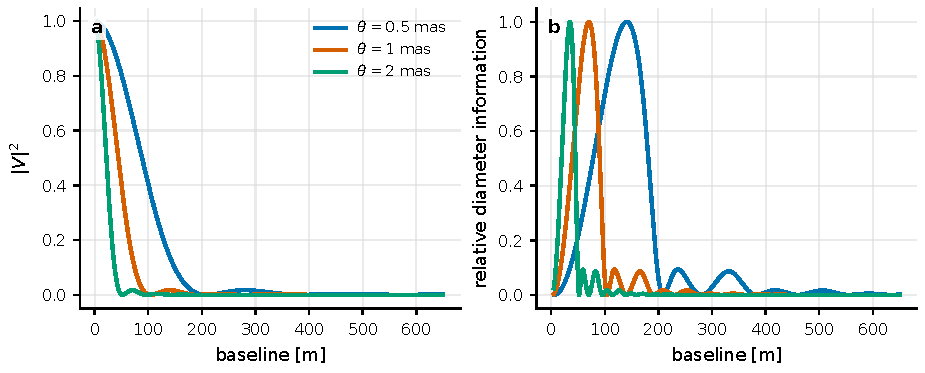
\includegraphics[width=0.94\linewidth]{figures/generated/chapter_18/ch18_visibility_fisher.pdf}
\caption{The squared visibility curve of a uniform disk and its diameter sensitivity. At 416 nm, the descending regions of 2 mas, 1 mas, and 0.5 mas targets fall on baselines of tens of metres, a hundred metres, and a few hundred metres respectively; the right panel shows that diameter information comes mainly from baselines with large curve slope, while the short-baseline plateau $|V|^2\simeq1$ is almost insensitive to the diameter.}
\label{fig:e15-vis}
\end{figure}

Writing this intuition as a formula is the Fisher information of Chapter~\ref{chap:e12}. For a single parameter $\theta$ and a set of independent baseline measurements $\mu_i=|V_i|^2$, the Fisher information and the attainable variance are

\begin{equation}
  I(\theta)=\sum_i
  \frac{1}{\sigma_i^2}
  \left(\frac{\partial\mu_i}{\partial\theta}\right)^{\!2},
  \qquad
  \sigma_\theta\ge\frac{1}{\sqrt{I(\theta)}} .
  \label{eq:e15-fisher}
\end{equation}
\begin{formulaexplain}
$\mu_i$: the observable on the $i$-th baseline (such as $|V_i|^2$). $\partial\mu_i/\partial\theta$: its sensitivity (slope) to the target parameter. $\sigma_i$: the error of that measurement. The right side is the Cramér--Rao lower bound. Baselines with large slope and small error contribute the most.
\end{formulaexplain}

This formula turns the preceding sentences into a computable criterion. Each baseline's contribution is \emph{slope squared divided by error squared}: a large slope $\partial\mu_i/\partial\theta$ and a small error $\sigma_i$ contribute much. So two kinds of "seemingly fine but useless" baselines are immediately exposed: a baseline with a very small error but near-zero slope (on the plateau) contributes almost nothing; a baseline with a very large slope but $|V|^2$ so low that the correlation peak is buried in noise, giving a huge $\sigma_i$, also cannot hold up the result. Note that $\sigma_i$ must include both the statistical noise (from Eq.~\eqref{eq:e15-snr}) and the systematic terms of the next section. The VERITAS observation of the rapid rotator $\gamma$ Cas is a living example: different projected baselines sample $|V|^2$ in different directions, and only then can the oblateness and long-axis direction be constrained; a single equivalent circular-disk diameter simply cannot describe such a non-axisymmetric target \citep{2025ApJ...995..191A,2024ApJ...966...28A}.

Band choice is decided along with it. The same physical baseline samples a spatial frequency about 1.9 times higher at 416 nm than at 800 nm: the blue end has higher resolution, but atmospheric transmission, mirror reflectivity, detector quantum efficiency, and oblique filter incidence are all harder to deal with. Spectral-line observations require a different ledger: one computes the line flux rather than the broadband magnitude. For hot stars and Be stars, H$\alpha$, helium lines, or metal lines may come from an emitting region larger than the continuum; using narrowband to separate the geometric structure and the velocity channels is worthwhile, but the event rate, filter leakage, and background of each channel must all be recomputed \citep{2012NewAR..56..143D,2021MNRAS.506.1585Z}.

\section{Error budget: the statistical floor and the systematic floor}
\label{sec:e15-error-budget}

Now we come to the most practical, and most often overlooked by outsiders, section of the whole chapter. A novice writing an observing proposal often reports only a signal-to-noise ratio and is done. But the signal-to-noise ratio governs only the \emph{statistical} noise, which falls all the way with integration time; what truly decides "how precisely you can actually measure" is often a layer of \textbf{systematic floor that does not fall with time}. Separating the two is the error budget.

For one parameter $\theta$ to be fit, add the various errors in quadrature:

\begin{equation}
  \sigma_\theta^2
  = \sigma_{\rm stat}^2
  + \sigma_{\rm bg}^2
  + \sigma_{\rm time}^2
  + \sigma_{\rm cal}^2
  + \sigma_{\rm model}^2 .
  \label{eq:e15-error-budget}
\end{equation}
\begin{formulaexplain}
$\sigma_\theta$: the total error of the target parameter. The right side is, in order, the statistical, background, time, calibration, and model error. When independent, they add in quadrature. This formula reminds you: reporting one signal-to-noise ratio is not enough; you must also say clearly where the error floor comes from.
\end{formulaexplain}

Spell out each term: what it is, with dimensions all converted to the units of $\theta$. $\sigma_{\rm stat}$ comes from the finite coincidence count or correlation-peak fit, the direct consequence of the signal-to-noise ratio of Eq.~\eqref{eq:e15-snr}. $\sigma_{\rm bg}$ comes from the uncertainty of the off-source interpolation and the dark current. $\sigma_{\rm time}$ comes from the clock, geometric delay, sampling, and peak shape. $\sigma_{\rm cal}$ comes from the calibrator star, the total system transmission, the filter, and polarization. $\sigma_{\rm model}$ comes from the source model itself: forcing a rapid rotator into a disk, forcing a spectral-line disk into a Gaussian, or ignoring a companion star all introduce this term.

The key physics is that they \emph{behave differently with time}. The statistical term obeys the shot-noise $\sqrt N$ law (Chapter~\ref{chap:e03}): the count $N\propto T$, so

\begin{equation}
  \sigma_{\rm stat}(T)=\frac{c_0}{\sqrt{T}} ,
  \qquad
  \sigma_{\rm sys}^2=\sigma_{\rm bg}^2+\sigma_{\rm time}^2
        +\sigma_{\rm cal}^2+\sigma_{\rm model}^2 ,
  \label{eq:e15-floor}
\end{equation}
\begin{formulaexplain}
$c_0$: a constant determined by the photon rate, visibility slope, etc. $\sigma_{\rm stat}\propto T^{-1/2}$ falls with exposure; $\sigma_{\rm sys}$ gathers the systematic terms that do not fall with time. The total error is the quadrature sum of the two.
\end{formulaexplain}

Here $c_0$ is a constant absorbing the photon rate, visibility slope, and calibration chain (with units consistent with $\theta$). The picture is clear: $\sigma_{\rm stat}$ is like a continuously sliding slope, lower the longer you expose; while $\sigma_{\rm sys}$ is a \emph{horizontal floor}. The total error is the quadrature sum of the two, initially dominated by the statistical slope and falling with $T$, until it hits the systematic floor and \emph{stops moving}. The moment of hitting is when the statistical term equals the systematic term:
\[
  \sigma_{\rm stat}(T_\star)=\sigma_{\rm sys}
  \;\Longrightarrow\;
  T_\star=\left(\frac{c_0}{\sigma_{\rm sys}}\right)^{2}.
\]
\textbf{Adding time beyond $T_\star$ is almost wasted}: the total error already hugs the systematic floor, and quadrupling $T$ again only halves the statistical term, which is already far below the floor and has no effect on the total error. This is the sentence that should be made clearest, and most written into a proposal, in a feasibility calculation: not "the longer the exposure the better," but "one should stop when the statistical term falls near the systematic floor, and the remaining precision must be won by lowering the systematic terms." Figure~\ref{fig:e15-budget} plots this behaviour of the slope hitting the floor.

\begin{figure}[tbp]
\centering
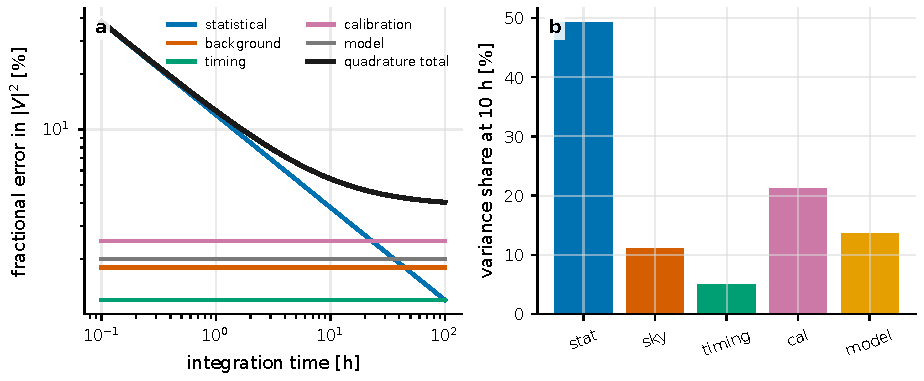
\includegraphics[width=0.94\linewidth]{figures/generated/chapter_18/ch18_error_budget.pdf}
\caption{The statistical and systematic terms in the error budget. Left: the statistical error falls with integration time, but the background, time, calibration, and model terms combine into a plateau; right: the contribution of each term to the total variance at 10 h. An observing proposal should connect every term to an observable calibration dataset, and give the error plateau in addition to the total signal-to-noise ratio.}
\label{fig:e15-budget}
\end{figure}

The most common and most easily quantified systematic term is \textbf{background dilution}. If there is, outside the source, a background light \emph{uncorrelated} with the signal (skyglow, moonlight, dark counts), it does not create a false correlation but proportionally lowers the true correlation peak. Let the ratio of background to starlight at one end be $\beta$; when symmetric at both ends, the observed contrast shrinks by $(1+\beta)^{-2}$ (Chapter~\ref{chap:e08}). Plug in numbers: at $\beta=0.03$ (background only 3\% of starlight), $(1.03)^{-2}=0.94$, only a 6\% drop, almost harmless; but at $\beta=0.5$, $(1.5)^{-2}=0.44$, the peak has only about forty percent left. The VERITAS analysis of $\beta$ UMa used off-source observations (off runs) about $0.5^\circ$ from the target to estimate the non-stellar-light current, with a typical off-source intensity only about 3\% of that on source, so the effect on the radius fit is small; but once there is a bright moon, cloud, fog, city light, or detector afterpulsing, this approximation worsens and separate quality slicing is required \citep{2024ApJ...966...28A,2025ApJ...995..191A}. Figure~\ref{fig:e15-bg} gives the dilution factor and its inverse correction.

\begin{figure}[tbp]
\centering
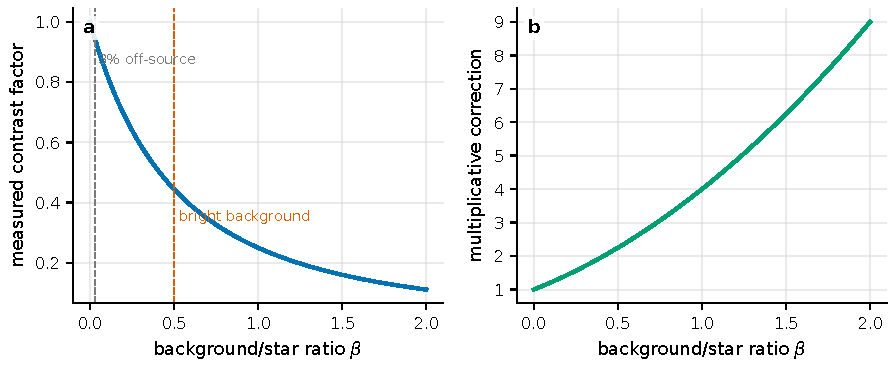
\includegraphics[width=0.94\linewidth]{figures/generated/chapter_18/ch18_background_dilution.pdf}
\caption{The dilution of the correlation peak by uncorrelated background. When the background/starlight ratio is the same at both ends, the observed contrast falls by $(1+\beta)^{-2}$: $\beta=0.03$ causes only a few percent correction, while $\beta=0.5$ has already pressed the peak to about 44\%. The right panel is the inverse correction factor; the larger the correction, the more sensitive it is to the background-estimate error.}
\label{fig:e15-bg}
\end{figure}

Time calibration is a hard boundary common to both intensity interferometry and photon counting. The correlation peak width is usually a few nanoseconds; if the relative delay model of the two telescopes is wrong by 1 ns, the peak is smeared wide, or even moved out of the fitting window. In the Vega photon-counting experiment, the relative time precision of the zero-baseline sub-apertures was about 100 ps, and between the two telescopes one still had to handle the light-travel time, instrument delay, GPS or rubidium clock drift, and fibre dispersion, finally correlating with a time bin of about 400 ps; they explicitly pointed out that a multi-telescope scheme must achieve about nanosecond-scale synchronization to keep the observation time at the hour scale. VERITAS uses White Rabbit's 10 MHz clock distribution plus 4 ns sampling, yet must still track the drift of the optical-path delay with hour angle within each run, and handle the run-to-run peak-position variation \citep{2021MNRAS.506.1585Z,2024ApJ...966...28A}.

The calibrator star must be chosen as carefully as the science target. An ideal calibrator should have a known angular diameter, stable luminosity, a sky position close to the target, a similar colour, and a sufficiently high photon rate. If the target is a 0.5 mas hot star, and the calibrator's own diameter has a 5\% uncertainty, then the final diameter error is easily dominated by this term $\sigma_{\rm cal}$, and exposing longer is of no use. Modern intensity-interferometry observations often first take a hot star of known angular diameter as a reference, check the zero-baseline normalization, filter response, and $|V|^2(B)$ shape, and then measure the unknown target. MAGIC's 2024 performance paper used several reference stars to validate the system and then gave new stellar angular diameters; VERITAS went from the disk diameter of $\beta$ UMa all the way to the oblateness and position angle of $\gamma$ Cas, using the same calibration framework \citep{2024MNRAS.529.4387A,2024ApJ...966...28A,2025ApJ...995..191A}.

\section{A feasibility calculation from beginning to end}
\label{sec:e15-worked}

Now let us string the whole chapter into one real calculation. Let the science goal be: \textbf{use a VERITAS-type array to measure the angular diameter of a hot, bright star, pressing the relative error to a few percent}. The array parameters are all taken from the real VERITAS intensity-interferometry system; the target is a hot star sitting at the edge of sensitivity, so that this problem is neither "easily measurable" nor "hopeless."

\textbf{Step 0: write down the target parameters and success criteria.} The physical quantity to measure is the angular diameter $\theta$, with target precision $\sigma_\theta/\theta\lesssim3\%$. The success criteria are quantified as: at least three baselines reach ${\rm SNR}>5$ in the descending region of the first lobe; the normalization drift of the repeated calibrator observations is less than 3\%; and the off-source background correction is less than 10\% of the total signal.

\textbf{Step 1: choose the target, fix the photon rate.} We deliberately pick a hypothetical early-type star at $m_V\approx5$ with effective temperature about $10^4\,{\rm K}$, fainter than VERITAS's real bright targets such as $\beta$ UMa ($m_V\approx2.4$) and $\gamma$ Cas ($m_V\approx2.2$) and sitting right at the edge of sensitivity, so that the problem is not too easy. (A reminder: the $m_V\approx5$, $T_{\rm eff}\approx10^4\,{\rm K}$, $\theta\approx0.7\,{\rm mas}$ used in this section are illustrative numbers given \emph{independently} to demonstrate each step, and need not correspond to the same real star: if one seriously plugs them into the Stefan--Boltzmann relation $f_{\rm bol}=\sigma T^4(\theta/2)^2$, one finds these three numbers are not strictly self-consistent, and the reader need not dwell on this.) Using the chain of Section~\ref{sec:e15-photon-budget}, a 12 m telescope at 550 nm, 10 nm passband, $\eta=0.25$ gives $R_\gamma\simeq2.8\times10^8\,{\rm s^{-1}}$. Switching to VERITAS's actual 416 nm, 13 nm filter, the photon rate is of the same order. Conclusion: photons are plentiful, and this star will not drop out for being too faint.

\textbf{Step 2: estimate the angular scale, fix the baseline.} A $10^4\,{\rm K}$ early-type bright star usually has an angular diameter of 0.5--1 mas. By Eq.~\eqref{eq:e15-baseline}, a star of $\theta\approx0.7\,{\rm mas}$ at 416 nm has its first-lobe descending region falling around $86/0.7\approx120\,{\rm m}$. VERITAS's six baselines from four 12 m telescopes cover tens of metres to about 170 m, exactly bracketing the descending region and near the first zero: this means we have several baselines falling where the \emph{slope is large}, satisfying the diameter-information criterion of Section~\ref{sec:e15-baseline}.

\textbf{Step 3: estimate the correlation-peak height and the statistical signal-to-noise ratio.} By Section~\ref{sec:e15-photon-budget}, 416 nm, 13 nm, 4 ns give $\tau_c\simeq4.4\times10^{-14}\,{\rm s}$, and the diluted zero-baseline peak is about a few $10^{-6}$. Substituting the array parameters into Eq.~\eqref{eq:e15-snr}: the equivalent LeBohec--Holder calculation shows that with $A=100\,{\rm m^2}$, $\alpha=0.3$, $\Delta f=1\,{\rm GHz}$, $|V|^2=0.5$, a star of $m_V\simeq6.7$ reaches $5\sigma$ in 5 h; our star at $m_V\approx5$ is about 5 times brighter, so the same 5 h single-baseline signal-to-noise ratio can soar past twenty. Taking a conservative single-baseline ${\rm SNR}\approx5$--$10$ is already sufficient.

\textbf{Step 4: translate the signal-to-noise ratio into the angular-diameter error.} The relative error of the correlation peak is $\sigma_{|V|^2}/|V|^2\approx1/{\rm SNR}$. To convert it into the angular-diameter error, use one \textbf{error propagation}: the observable $|V|^2$ is a function of $\theta$, and a small error in $\theta$ is carried by the derivative into an error in $|V|^2$,
\[
  \sigma_{|V|^2}=\left|\frac{\partial|V|^2}{\partial\theta}\right|\,\sigma_\theta .
\]
Dividing both sides by $|V|^2$ and $\theta$, the right side neatly assembles into the logarithmic derivative $\partial\ln|V|^2/\partial\ln\theta=(\theta/|V|^2)\,\partial|V|^2/\partial\theta$, so
\[
  \frac{\sigma_\theta}{\theta}
  =\frac{\sigma_{|V|^2}/|V|^2}{\left|\partial\ln|V|^2/\partial\ln\theta\right|} .
\]
In the descending region, the \emph{logarithmic slope} of the visibility with respect to the diameter $|\partial\ln|V|^2/\partial\ln\theta|$ is of order 1--2; substituting $\sigma_{|V|^2}/|V|^2\approx1/{\rm SNR}$ gives
\[
  \frac{\sigma_\theta}{\theta}
  \approx\frac{1}{{\rm SNR}}\,
  \frac{1}{\left|\partial\ln|V|^2/\partial\ln\theta\right|}
  \approx\frac{1}{5}\times\frac{1}{1.5}
  \approx13\%
\]
That is, a \emph{single} large-slope baseline gives about a dozen percent in 5 h. Then use Eq.~\eqref{eq:e15-fisher} to add the information of multiple baselines: $N_b$ equally useful baselines shrink the statistical error by $1/\sqrt{N_b}$, and if three of the six baselines fall in the descending region, $\sigma_\theta/\theta$ is pressed to about $13\%/\sqrt3\approx7\%$; adding a few more nights, or the more baselines of more telescopes, makes reaching 3\% realistic. This step turns "signal-to-noise ratio" genuinely into "to what fraction of a percent the angular diameter can be measured."

\textbf{Step 5: check the error budget, decide whether to keep exposing.} Use Eq.~\eqref{eq:e15-error-budget} and \eqref{eq:e15-floor} to check the systematic floor. Background: off-source $\beta\approx0.03$, a dilution correction of about 6\%, calibratable by off-source observations, so $\sigma_{\rm bg}$ is small. Time: White Rabbit plus 4 ns sampling, relative delay controlled at the nanosecond scale, so $\sigma_{\rm time}$ is manageable. Calibration: if the calibrator's diameter is known to 3\%, then $\sigma_{\rm cal}$ is about 3\%, which is exactly of the same order as our target precision, becoming the \textbf{most likely systematic floor}. By Eq.~\eqref{eq:e15-floor}, when the statistical term $\sigma_{\rm stat}$ is exposed down to about 3\% (corresponding to $T_\star$), the total error hugs this floor set by the calibrator, and \emph{adding more exposure is meaningless}. The conclusion is plain: whether this observation can reach 3\% depends in the end not on exposing a few more hours, but on \emph{whether there is a calibrator with a sufficiently well-determined diameter}.

\textbf{Step 6: write it into the feasibility conclusion of the proposal.} One sentence to close: for a hot star of $m_V\approx5$, $\theta\approx0.7\,{\rm mas}$, using VERITAS's six baselines, 416 nm/13 nm, 4 ns sampling, several nights of effective exposure can reach ${\rm SNR}>5$ on multiple baselines in the descending region, pressing the angular-diameter statistical error to about 3\%; the systematic floor is dominated by the calibrator's diameter uncertainty (about 3\%), so the upgrade direction is not longer exposure, but a better calibrator and stricter filter/background control. If no correlation is detected on the longest baseline, one can still give an \emph{upper limit} on the angular diameter or rule out an emitting region too large: returning empty-handed is also a valuable result.

This estimation chain is not exclusive to intensity interferometry. Amplitude interferometry, the quantum-network telescope, CMB polarization, and the photon statistics of fast radio bursts (FRBs), down to a laboratory teaching bench, all use the same skeleton: event rate $\to$ number of modes $\to$ response function $\to$ calibration terms $\to$ model derivatives $\to$ error budget; the difference is only in the specific form of the observable $\mu_i$. The ranking of science cases should also follow this line of thought, scoring "scientific value" and "observability" separately in two columns, and not conflating a \emph{beautiful} target with a \emph{doable} one \citep{2010SPIE.7734E..0AD,2012MNRAS.419..172N,2013APh....43..331D,2022SPIE12183E..0DK}. Table~\ref{tab:e15-checklist} lists the common ranges and uses of each quantity in this ledger as a checklist.

\begin{longtable}{p{0.16\linewidth}p{0.30\linewidth}p{0.44\linewidth}}
\caption{Feasibility-ledger quick-reference table: the common range and planning use of each quantity.}
\label{tab:e15-checklist}\\
\toprule
Quantity & Common range & Use in the plan \\
\midrule
\endfirsthead
\toprule
Quantity & Common range & Use in the plan \\
\midrule
\endhead
$m_V,\,m_B$ & $-1$ to $9$ mag, the current main battleground of intensity interferometry & Convert to $R_\gamma$ via Eqs.~\eqref{eq:e15-ab-flux} and \eqref{eq:e15-photon-rate}, first judging whether the target is too faint. \\
$A_{\rm eff}$ & $1$--$250\,{\rm m^2}$ per telescope & Enters the photon rate and signal-to-noise ratio; mirror ageing, obscuration, and fibre coupling must all be folded into the efficiency. \\
$\Delta\lambda$ & $0.1$--$30\,{\rm nm}$ & Determines the coherence time, PMT current, sky background, and spectral-line selection. \\
$\Delta t$ & $0.1$--$5\,{\rm ns}$ & Determines the degree of correlation-peak dilution and the usable electronic bandwidth. \\
$B_p$ & $10$--$2000\,{\rm m}$ & Determines the angular scale and $u,v$ coverage; short and long baselines constrain different structures. \\
$\beta$ & $0.01$--$1$ & The background/starlight ratio, determining the contrast dilution and the background systematic error. \\
$\sigma_{\rm cal}$ & $1\%$--$10\%$ of the visibility or diameter & Often becomes the error floor after long exposure. \\
\bottomrule
\end{longtable}

\section{Chapter Summary}
\label{sec:e15-summary}

\begin{itemize}
  \item \textbf{An observation is a ledger.} Eq.~\eqref{eq:e15-likelihood} connects the physical parameters to the data via "instrument observable + calibration + background"; designing an observation is computing this chain segment by segment into real numbers, not merely writing "which star to look at." The event table is the raw broth, the image is the boiled-down spoonful: information averaged away at recording cannot be recovered.
  \item \textbf{The photon budget has four steps.} Magnitude $\to$ spectral flux density (Eq.~\eqref{eq:e15-ab-flux}) $\to$ photon flux per unit area $\to$ multiply by area and efficiency to get the effective photon rate (Eq.~\eqref{eq:e15-photon-rate}). A 12 m telescope gives $R_\gamma\simeq2.8\times10^8\,{\rm s^{-1}}$ for an $m_{\rm AB}=5$ star; but coherence dilution $\tau_c/\Delta t\sim10^{-5}$ presses the zero-baseline peak to a few $10^{-6}$.
  \item \textbf{Signal-to-noise accumulates as $\sqrt T$.} In Eq.~\eqref{eq:e15-snr}, ${\rm SNR}\propto A\alpha n|V|^2\sqrt{\Delta f\,T}$; $A\alpha n$ is the photon degeneracy $\delta\sim10^{-4}$--$10^{-2}$. Because $n$ is a spectral density, widening the optical passband earns almost no free signal-to-noise. To double the precision, one must expose four times as long.
  \item \textbf{The baseline is chosen by the visibility slope.} Diameter information is concentrated in the descending region where $|\partial|V|^2/\partial\theta|$ is largest (Eq.~\eqref{eq:e15-fisher}); a baseline on the plateau with near-zero slope contributes nothing however small its error, and a baseline with $|V|^2$ too low is buried in noise however large its slope.
  \item \textbf{Error budget $=$ statistical floor $+$ systematic floor.} Eqs.~\eqref{eq:e15-error-budget} and \eqref{eq:e15-floor}: $\sigma_{\rm stat}\propto T^{-1/2}$ slides all the way down, while the systematic terms (background, time, calibration, model) are a horizontal floor. After exposing to $T_\star=(c_0/\sigma_{\rm sys})^2$, once the statistical term hits the floor, \emph{adding more exposure is meaningless}: the remaining precision must be won by lowering the systematic terms.
  \item \textbf{The feasibility calculation has a fixed routine.} Target parameters $\to$ photon rate $\to$ baseline $\to$ signal-to-noise ratio $\to$ angular-diameter error $\to$ error-budget stopping decision. This skeleton applies equally to amplitude interferometry, the quantum-network telescope, CMB polarization, and FRB photon statistics, with the difference only in the form of the observable.
\end{itemize}

\medskip
\noindent\textbf{Questions to Ponder.}
(1) If the optical passband is widened from 10 nm to 30 nm, the photon rate rises 3 times, yet the intensity-interferometry signal-to-noise ratio barely moves: explain why using the fact that $n$ in Eq.~\eqref{eq:e15-snr} is a spectral density.
(2) You have exposed for 5 h with a statistical error of 4\%, but the calibrator diameter is known only to 3\%. Is it worth exposing to 20 h? Use Eq.~\eqref{eq:e15-floor} to compute from what to what the total error would fall.
(3) A star's angular diameter is estimated at 0.3 mas, and the longest baseline you have is only 100 m (416 nm). Which section of the visibility curve do you fall on? Is this baseline sensitive to the diameter? Should you seek a longer or a shorter baseline?


% ============================================================
\part{Astrophysical Objects as Quantum Light Sources}
\chapter{The Quantum Language of Astrophysical Radiation Mechanisms}
\label{chap:e16}

\begin{chapteropening}
By this point we have assembled a complete quantum toolkit for light: how many photons a mode contains on average (the Bose occupation number \(\bar n_\nu\) of Chapter~\ref{chap:e05}), what quantum state those photons form (the number, coherent, and thermal states of Chapter~\ref{chap:e06}), and how to tell the states apart using the second-order coherence function \(g^{(2)}\) (Chapter~\ref{chap:e08}). Now, for the first time, we truly point a telescope at the sky. A star, an HII region, a jet, a maser spot, a fast radio burst: each of them ultimately leaves an \(I_\nu\) spectrum on the detector; yet the photon-field statistics behind them can differ enormously. This chapter opens Part~4 of the book, and its task is a single sentence: to translate the whole zoo of astrophysical radiation mechanisms into the one language of ``mode occupation number + photon statistics,'' making clear which mechanisms are born as chaotic thermal light, which may deviate, and why capturing a genuinely nonclassical beam of light from an astrophysical source is so hard.
\end{chapteropening}

\section{Translating Radiation Mechanisms into Occupation Number and Photon Statistics}
\label{sec:e16-translation}

The traditional entry point to radiation mechanisms is the specific intensity \(I_\nu\), the radiant energy flux passing through per unit time, unit area, unit frequency, and unit solid angle, with CGS units \({\rm erg\,s^{-1}\,cm^{-2}\,Hz^{-1}\,sr^{-1}}\). If the source subtends a solid angle \(\Omega_{\rm s}\) on the sky, the flux density received by the telescope is approximately \(S_\nu\simeq I_\nu\,\Omega_{\rm s}\), commonly measured in Jy (\(1~{\rm Jy}=10^{-23}~{\rm erg\,s^{-1}\,cm^{-2}\,Hz^{-1}}\)). When textbooks treat radiation mechanisms, they usually stop at this spectrum \(I_\nu(\nu)\).

The trouble is that the spectrum is only an ``average.'' You can build the very same \(I_\nu\) spectrum out of completely different light fields. Picture two ponds whose surfaces ripple with waves of the same height: in one pond the ripples come from countless raindrops each splashing independently and adding incoherently; in the other, someone stands at the shore slapping the water rhythmically, so that many wave crests are pushed out in step. Standing far away and measuring the ``average ripple height,'' the two ponds look identical; but the moment you watch the way the surface \emph{fluctuates}, they part ways at once. Astrophysical radiation is the same: the mean spectrum \(I_\nu\) erases the correlations in photon arrival times, the correlations in polarization, and the joint probabilities among frequency channels, and it is precisely these that carry the fingerprint of the radiation mechanism.

To quantify these fingerprints, we recall the two coherence functions built up in the preceding two chapters. Let \(\hat E^{(+)}(t)\) be the positive-frequency electric-field operator (it corresponds to ``annihilating one photon,'' see Chapter~\ref{chap:e05}), and \(\hat E^{(-)}(t)=[\hat E^{(+)}(t)]^\dagger\). The normalized first-order coherence function is
\begin{equation}
  g^{(1)}(\tau)=
  \frac{\langle \hat E^{(-)}(t)\,\hat E^{(+)}(t+\tau)\rangle}
       {\langle \hat E^{(-)}(t)\,\hat E^{(+)}(t)\rangle},
  \label{eq:e16-g1}
\end{equation}
\begin{formulaexplain}
\(g^{(1)}(\tau)\) is the normalized first-order coherence function, dimensionless. The numerator correlates the field at the two instants \(t\) and \(t+\tau\); the denominator is the mean intensity. It measures how much the field's phase still ``remembers'' after a delay \(\tau\): \(|g^{(1)}|\) falls from 1 (fully coherent) to 0 (fully forgetful).
\end{formulaexplain}
The numerator \(\langle \hat E^{(-)}(t)\hat E^{(+)}(t+\tau)\rangle\) couples the field at the two instants, the denominator \(\langle \hat E^{(-)}(t)\hat E^{(+)}(t)\rangle\) is the mean intensity, and dividing one by the other gives a dimensionless quantity. \(|g^{(1)}(\tau)|\) decays from 1 at \(\tau=0\) to 0 at large \(\tau\), and the timescale of that decay is the coherence time \(\tau_c\simeq1/\Delta\nu\) (Chapter~\ref{chap:e02}). It governs the physics at the level of amplitude interferometry, line width, and visibility.

The second-order coherence function asks a different question, not ``does the phase still remember,'' but ``once one photon has arrived, will it bring another'':
\begin{equation}
  g^{(2)}(\tau)=
  \frac{\langle :\!\hat I(t)\,\hat I(t+\tau)\!:\rangle}{\langle \hat I(t)\rangle^2},
  \label{eq:e16-g2}
\end{equation}
\begin{formulaexplain}
\(g^{(2)}(\tau)\) is the normalized intensity correlation, dimensionless; \(\hat I(t)\) is the instantaneous intensity operator, and the colons denote normal ordering (annihilation operators placed to the right). It compares the joint probability of photon arrivals at the two instants against the independent case: \(>1\) bunching, \(=1\) Poisson, \(<1\) antibunching.
\end{formulaexplain}
Here \(\hat I(t)\propto\hat E^{(-)}(t)\hat E^{(+)}(t)\) is the instantaneous intensity, and the colons \(:\ :\) denote normal ordering (all \(\hat a^\dagger\) placed to the left of \(\hat a\), which removes the shot noise of the detection process itself, see Chapter~\ref{chap:e08}). \(g^{(2)}(\tau)\) is dimensionless, and its physics is a ``conditional probability'': given that a photon is detected at time \(t\), how much higher (relative to the independent case) is the probability of detecting another at \(t+\tau\): higher (\(>1\), bunching), the same (\(=1\), Poisson), or lower (\(<1\), antibunching, found only in nonclassical light).

Chapters~\ref{chap:e06} and~\ref{chap:e08} already worked out the value at \(\tau=0\) for three reference states, and we quote them here as known results: for a \emph{single-mode thermal (chaotic) state} \(g^{(2)}(0)=2\), for a \emph{coherent state} \(g^{(2)}(0)=1\), and for a \emph{number state} \(g^{(2)}(0)<1\). These are the three yardsticks of this chapter. The core work of the whole chapter is to place each astrophysical radiation mechanism between these three yardsticks: where does it fall by default? under what conditions does it deviate? and, most crucially, where will a real observation compress it to?

\section{Brightness Temperature: Converting Mean Intensity into Occupation Number}
\label{sec:e16-brightness}

Before we start translating mechanisms, we need a bridge that converts the directly observed \(I_\nu\) into the mode occupation number \(\bar n_\nu\) of Chapter~\ref{chap:e05}. That bridge is the \emph{brightness temperature} \(T_b\).

In the Rayleigh--Jeans form common in the radio and far-infrared, one inverts \(I_\nu\) into an ``equivalent temperature'':
\begin{equation}
  T_b=\frac{c^2\,I_\nu}{2k_B\nu^2}
      =\frac{c^2\,S_\nu}{2k_B\nu^2\,\Omega_{\rm s}} .
  \label{eq:e16-brightness-temperature}
\end{equation}
\begin{formulaexplain}
\(T_b\) is the brightness temperature, in K; \(c\) the speed of light, \(k_B\) the Boltzmann constant, \(\nu\) the frequency, \(\Omega_{\rm s}\) the source solid angle. It answers ``if this bit of radiation came from a blackbody in the R--J limit, how hot would that blackbody have to be.'' It is not the true temperature of the matter.
\end{formulaexplain}
Here \(c\) is the speed of light, \(k_B=1.38\times10^{-16}~{\rm erg\,K^{-1}}\) is the Boltzmann constant, and \(\nu\) is the frequency. The unit of \(T_b\) is K, but keep firmly in mind: it is a \emph{defined} equivalent quantity, answering the question ``if this \(I_\nu\) came from a Rayleigh--Jeans-limit blackbody, how hot would the blackbody be.'' For nonthermal electrons, masers, or FRBs, \(T_b\) is not at all equal to the thermal temperature of the matter; it can be higher than any physical temperature could ever reach. Note that \(T_b\propto S_\nu/\Omega_{\rm s}\): the smaller the source on the sky, the higher the \(T_b\) implied by the same flux density, so angular-size measurements (VLBI), variability timescales, and scattering broadening all feed directly into the mechanism judgment.

Now let us connect this bridge to the quantum side. The blackbody specific intensity for one polarization and one frequency mode is the Planck function \(B_\nu=(2h\nu^3/c^2)\,\bar n_\nu\), where the occupation number
\[
  \bar n_\nu=\frac{1}{\exp(h\nu/k_BT)-1}
\]
is precisely the protagonist of Chapter~\ref{chap:e05}. Substituting \(I_\nu=B_\nu\) into the brightness-temperature definition~\eqref{eq:e16-brightness-temperature}, the \(2\nu^2/c^2\) on both sides cancels, and we obtain directly an extremely clean correspondence:
\begin{equation}
  \bar n_\nu=\frac{k_B T_b}{h\nu}
  \qquad(\text{exact under the Rayleigh--Jeans definition}).
  \label{eq:e16-occupation-from-tb}
\end{equation}
\begin{formulaexplain}
\(\bar n_\nu\) is the mean photon number in a single spacetime--polarization mode; \(k_B T_b\) is the energy corresponding to the brightness temperature, and \(h\nu\) is the single-photon energy. This equation says: \emph{brightness temperature is essentially the occupation number}, the two differing only by the conversion factor \(h\nu/k_B\).
\end{formulaexplain}
This step is the ``Rosetta Stone'' of the chapter: \(\bar n_\nu=k_B T_b/(h\nu)\). Brightness temperature is nothing but the mode occupation number wearing a ``temperature'' coat. High \(T_b\) means every mode is stuffed with photons; low \(T_b\) means the modes are nearly empty. In one glance this welds the ``mean spectrum'' to the ``quantum occupation number.''

Plug in two real numbers and the sense of scale comes out at once. First, the \emph{stellar photosphere in the visible}: taking \(T\simeq6000~{\rm K}\) and \(\nu\simeq6\times10^{14}~{\rm Hz}\) (\(\lambda\simeq500~{\rm nm}\)), we get \(h\nu/k_BT=(6.6\times10^{-27}\times6\times10^{14})/(1.38\times10^{-16}\times6000)\simeq4.8\), which lies in the Wien regime rather than the R--J regime, giving occupation number \(\bar n_\nu=1/(e^{4.8}-1)\simeq0.008\). On average, each mode holds only a hundredth of a photon! This explains why the visible light of a star is an extremely ``dilute'' beam, why the Hanbury Brown--Twiss bunching signal is so faint, and why the photon rate is the lifeline of interstellar measurements (Chapter~\ref{chap:e10}). Second, the \emph{FRB}: a millisecond, Jy-level, Gpc-distance, GHz-frequency radio pulse, substituted into~\eqref{eq:e16-brightness-temperature}, gives
\begin{equation}
  T_b\simeq
  1.1\times10^{35}~{\rm K}
  \left(\frac{S_\nu}{1~{\rm Jy}}\right)
  \left(\frac{D_A}{1~{\rm Gpc}}\right)^2
  \left(\frac{t_{\rm FRB}}{1~{\rm ms}}\right)^{-2}
  \left(\frac{\nu}{1~{\rm GHz}}\right)^{-2},
  \label{eq:e16-frb-tb}
\end{equation}
\begin{formulaexplain}
\(S_\nu\) the pulse flux density, \(D_A\) the angular-diameter distance, \(t_{\rm FRB}\) the pulse width, \(\nu\) the observing frequency. This astronomical number shows that the brightness temperature of a millisecond FRB far exceeds the upper limit any incoherent radiation can reach.
\end{formulaexplain}
where \(D_A\) is the angular-diameter distance (the pulse width \(t_{\rm FRB}\) sets an upper bound on the source size through the causality limit \(\Omega_{\rm s}\lesssim(c\,t_{\rm FRB}/D_A)^2\)). Substituting \(T_b\sim10^{35}~{\rm K}\) and \(\nu=1~{\rm GHz}\) into~\eqref{eq:e16-occupation-from-tb}: \(\bar n_\nu\simeq k_BT_b/(h\nu)=(1.38\times10^{-16}\times10^{35})/(6.6\times10^{-27}\times10^{9})\simeq2\times10^{36}\). Each mode is crammed with \(10^{36}\) photons; this can no longer be explained by ``many independent particles each radiating on their own''; it requires an enormous number of charged particles to \emph{cooperatively} emit on scales smaller than a wavelength or with controlled phase \citep{2007Sci...318..777L,2019A&ARv..27....4P,2022A&ARv..30....2P}. Here the occupation number shouts the word ``coherence'' on our behalf.

\begin{figure}[tbp]
\centering
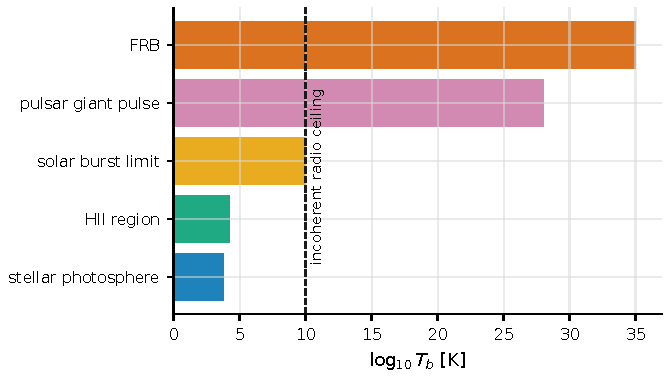
\includegraphics[width=0.82\linewidth]{figures/generated/chapter_09/ch09_brightness_temperature_scale.pdf}
\caption{Brightness temperature as the first-level criterion for radiation mechanisms. Stellar photospheres and HII regions fall in the ordinary thermal-temperature range (corresponding to occupation number \(\bar n_\nu\lesssim1\)); solar and stellar radio bursts exceeding \(10^{10}~{\rm K}\) often require a coherent mechanism; the brightness temperatures of pulsar giant pulses and FRBs are higher still (occupation number up to \(10^{30}\) and beyond) and can only be explained by coherent emission or strong beaming geometry. The dashed line marks the order of magnitude of the commonly used incoherent-radio limit.}
\label{fig:e16-brightness-temperature}
\end{figure}

Brightness temperature gives us a hard, empirical threshold. Dulk's review of solar and stellar radio emission provides a practical criterion: the \(T_b\) of incoherent radio emission can hardly exceed \(10^9\)--\(10^{10}~{\rm K}\), an upper limit set mainly by gyrosynchrotron self-absorption and energetic constraints (once the occupation number is too high, self-absorption and radiation reaction push it back down; incidentally, the inverse-Compton catastrophe of Kellermann--Pauliny-Toth gives a higher scale of \(\sim10^{12}~{\rm K}\), and the two should not be confused); bursts significantly above this range must invoke a coherent mechanism, such as plasma emission or the electron-cyclotron maser \citep{1985ARA&A..23..169D}. The brightness-temperature yardstick (Figure~\ref{fig:e16-brightness-temperature}) thus becomes the first cut in mechanism judgment: is the occupation number the \(\lesssim1\) of ``dilute thermal light,'' or the \(10^{20}\), \(10^{30}\) of a ``coherent burst''? But this is only the first cut: it only checks whether the mean energy density is reasonable, and says nothing about whether these photons add up independently or emit cooperatively. To settle that step, we must call upon photon statistics.

\section{Why Thermal Radiation Is Born as Chaotic Light}
\label{sec:e16-thermal}

Consider first the most ``well-behaved'' entry in the family tree: thermal radiation. Stellar photospheres, dust, HII regions, and the cosmic microwave background are all approximately in local thermodynamic equilibrium. Their mode occupation numbers are given by the Planck distribution,
\begin{equation}
  \bar n_\nu=\frac{1}{\exp(h\nu/k_BT)-1},
  \label{eq:e16-planck-occupation}
\end{equation}
\begin{formulaexplain}
\(\bar n_\nu\) the mean occupation number of the mode at frequency \(\nu\); \(h\nu\) the single-photon energy, \(T\) the temperature of the matter. In the R--J regime (\(h\nu\ll k_BT\)), \(\bar n_\nu\approx k_BT/h\nu\gg1\); in the Wien regime (\(h\nu\gg k_BT\)), \(\bar n_\nu\approx e^{-h\nu/k_BT}\ll1\).
\end{formulaexplain}
Here \(T\) is the thermal temperature of the matter. Note that the visible light of a stellar photosphere often lies in the Wien regime (\(h\nu/k_BT>1\)), so color temperature, effective temperature, and brightness temperature must not be conflated: for the same star, \(\bar n_\nu\) is large at the radio end and small at the optical end. But whichever regime it falls in, the \emph{statistical properties} of the thermal state are the same, and this is precisely what we care about.

Why is thermal radiation born as chaotic light? The physical picture is this: a thermal source contains an enormous number of independent emitters (atoms, ions, electrons), each emitting a small wave train at a random time with a random phase. The total electric field reaching the detector is the vector sum of these millions upon millions of little arrows with random phases and random amplitudes. Here the central limit theorem enters (the sum of a large number of independent random quantities tends to a Gaussian distribution), so within a narrow band the complex electric field \(\hat E^{(+)}(t)\) is a \emph{complex Gaussian random process}. This is no coincidence; it is the inevitable consequence of ``adding up many independent events.''

A Gaussian random process has a beautiful algebraic property (proved in Chapter~\ref{chap:e08}, quoted here as a known result): its fourth-order moment can be decomposed into products of second-order moments (the moment theorem / Gaussian moment theorem). Applying this property to the numerator of~\eqref{eq:e16-g2} yields the Siegert relation
\begin{equation}
  g^{(2)}(\tau)=1+\frac{|g^{(1)}(\tau)|^2}{M_{\rm eff}},
  \label{eq:e16-siegert}
\end{equation}
\begin{formulaexplain}
The Siegert relation: the second-order coherence of chaotic (Gaussian) light is fully determined by its first-order coherence. \(M_{\rm eff}\) is the number of modes averaged over simultaneously. The single-mode case (\(M_{\rm eff}=1\), \(\tau=0\)) gives \(g^{(2)}(0)=1+1=2\), the thermal-light bunching peak.
\end{formulaexplain}
In a single spacetime--polarization mode (\(M_{\rm eff}=1\)) at \(\tau=0\), since \(|g^{(1)}(0)|=1\), we immediately obtain \(g^{(2)}(0)=1+1=2\). This is the seed of thermal-light bunching, and the anchor point we will use again and again in this chapter: \emph{as long as it is ``many independent emitters added together,'' the light field is a Gaussian chaotic field, and it automatically carries the \(g^{(2)}(0)=2\) bunching peak.} Thermal light is not mysterious; its bunching is purely the statistical consequence that ``the intensity clumps and fluctuates'' when random-phase amplitudes superpose.

The power of this logic lies in its \emph{indifference to mechanism}. As long as ``many independent events add up and the phase is random within a narrow band'' is satisfied, the shape of the spectrum is irrelevant: the conclusion is always Gaussian chaotic light. The first example is \emph{free-free radiation} (bremsstrahlung): it is not the blackbody spectrum itself but the continuous spectrum from countless electrons being accelerated in the Coulomb fields of ions, each emitting one burst of braking radiation. The phase of a single collision is completely unpredictable, and the complex field within a narrow band still tends to a Gaussian process. In a thin ionized gas, the emission coefficient scales as
\begin{equation}
  j_\nu^{\rm ff}\propto
  n_e\,n_i\,T_e^{-1/2}
  \exp\!\left(-\frac{h\nu}{k_BT_e}\right)
  g_{\rm ff}(\nu,T_e),
  \label{eq:e16-free-free}
\end{equation}
\begin{formulaexplain}
\(j_\nu^{\rm ff}\) the free-free emission coefficient; \(n_e,n_i\) the electron and ion number densities (\({\rm cm^{-3}}\)), \(T_e\) the electron temperature, \(g_{\rm ff}\) the Gaunt factor (\(\sim1\) to a few tens). It is a continuous spectrum contributed by many independent Coulomb collisions.
\end{formulaexplain}
where \(n_e,n_i\) are the electron and ion number densities (\({\rm cm^{-3}}\)), \(T_e\) is the electron temperature, and \(g_{\rm ff}\) is the Gaunt factor. HII regions have \(T_e\sim10^4~{\rm K}\); stellar winds and accretion flows can be hotter. The spectral shape (nearly flat at the radio end, exponentially declining at high frequency) is completely different from a blackbody, but the photon statistics are the same chaotic thermal light, likewise carrying the seed \(g^{(2)}(0)=2\).

Still, for the spectrum to be observed it must pass through the medium, which brings in the radiative transfer equation:
\begin{equation}
  \frac{{\rm d}I_\nu}{{\rm d}s}=j_\nu-\alpha_\nu I_\nu,
  \qquad
  S_\nu=\frac{j_\nu}{\alpha_\nu}.
  \label{eq:e16-radiative-transfer}
\end{equation}
\begin{formulaexplain}
\({\rm d}I_\nu/{\rm d}s\) the change of intensity along the line of sight; \(j_\nu\) adds radiation, \(\alpha_\nu I_\nu\) absorbs it, and \(S_\nu=j_\nu/\alpha_\nu\) is the source function. It links the emission mechanism to the optical depth.
\end{formulaexplain}
\(s\) is distance along the line of sight, \(j_\nu\) is the emission coefficient, \(\alpha_\nu\) is the absorption coefficient, and the source function is \(S_\nu=j_\nu/\alpha_\nu\). Defining the optical depth \({\rm d}\tau_\nu=\alpha_\nu\,{\rm d}s\) and integrating~\eqref{eq:e16-radiative-transfer} over a uniform slab (this is a first-order linear ODE, solved directly with the integrating factor \(e^{\tau_\nu}\), a standard result), then converting to brightness temperature, we get
\begin{equation}
  T_b=T_{\rm eff}\left(1-e^{-\tau_\nu}\right)+T_{\rm bg}\,e^{-\tau_\nu}.
  \label{eq:e16-tb-transfer}
\end{equation}
\begin{formulaexplain}
\(T_b\) the emergent brightness temperature; \(T_{\rm eff}\) the temperature corresponding to the source function, \(T_{\rm bg}\) the background brightness temperature, \(\tau_\nu\) the optical depth. A thin source (\(\tau_\nu\ll1\)) adds only a little; a thick source (\(\tau_\nu\gg1\)) tends toward its own source function.
\end{formulaexplain}
For small optical depth \(T_b\simeq T_{\rm eff}\tau_\nu+T_{\rm bg}\) (a thin source contributes only a small increment), and for large optical depth \(T_b\to T_{\rm eff}\) (a thick source thermalizes to its own source function). This equation is commonly used to judge whether a source is thermalized, semi-transparent, or nonthermal-dominated \citep{1979rpa..book.....R,2011piim.book.....D,1985ARA&A..23..169D}. It also explains where the brightness-temperature upper limit comes from: once the optical depth is large enough, \(T_b\) is pinned by the source function (for a thermal source, the matter temperature) and cannot climb higher.

To summarize the physics of this section: what thermal and free-free radiation have in common is not the spectral shape but the statistical root of ``many independent emitters added together.'' This root makes their fields Gaussian chaotic fields, both sitting by default at \(g^{(2)}(0)=2\). This is our ``zero point'': every other mechanism that follows will be measured by whether it stays at this setting or deviates from it.

\section{Nonthermal Particles: Spectrum and Polarization Change, but the Statistics Often Do Not}
\label{sec:e16-nonthermal}

One of the easiest mistakes a beginner makes is to equate ``nonthermal'' with ``non-Gaussian statistics.'' This section is devoted to dispelling that. Synchrotron and inverse-Compton radiation: their \emph{spectrum and polarization} do indeed depart completely from a blackbody, but their \emph{photon statistics} are for the most part still Gaussian chaotic light. The reason is again that same root: as long as the emitters are many independent particles with random phase within a narrow band, the central limit theorem still compresses the field into a Gaussian process.

Synchrotron radiation comes from relativistic electrons spiraling in a magnetic field. The characteristic frequency of a single electron is
\begin{equation}
  \nu_c=\frac{3eB\sin\alpha}{4\pi m_ec}\,\gamma^2 ,
  \label{eq:e16-synch-critical}
\end{equation}
\begin{formulaexplain}
\(\nu_c\) the synchrotron characteristic frequency; \(e\) the elementary charge, \(B\) the magnetic field, \(\alpha\) the pitch angle, \(m_e\) the electron mass, \(\gamma\) the Lorentz factor. The frequency grows with \(B\) and \(\gamma^2\), so high-energy electrons can push the radiation to very high frequency bands.
\end{formulaexplain}
where \(e\) is the elementary charge, \(B\) the magnetic field strength, \(\alpha\) the pitch angle, \(m_e\) the electron mass, and \(\gamma\) the Lorentz factor. A word of caution: the bare symbol \(\alpha\) here refers specifically to the pitch angle (the angle between the electron velocity and the magnetic field); do not confuse it with the absorption coefficient \(\alpha_\nu\) of the previous section or the synchrotron spectral index \(\alpha_{\rm syn}\) that appears below; the three are distinguished by context and subscript. Plug in numbers: \(B=1~{\rm G}\), \(\gamma=10^3\), \(\sin\alpha=1\) gives \(\nu_c\simeq4.2\times10^{12}~{\rm Hz}\) (far-infrared); switching to the weak fields of intergalactic or jet scales, \(B=10^{-5}~{\rm G}\), the same electrons radiate mainly in the radio. The emission coefficient of a real source is the superposition of contributions from electrons of all energies,
\begin{equation}
  j_\nu^{\rm syn}=\int P_\nu(E,B,\alpha)\,N(E)\,{\rm d}E ,
  \label{eq:e16-synch-emissivity}
\end{equation}
\begin{formulaexplain}
\(j_\nu^{\rm syn}\) the synchrotron emission coefficient; \(P_\nu\) the single-electron power spectrum, \(N(E)\) the electron energy distribution. The integral shows that the observed spectrum is the sum of contributions from electrons of all energies: precisely ``many independent emitters added together.''
\end{formulaexplain}
If the electron energy spectrum is a power law \(N(E)\propto E^{-p}\), optically thin synchrotron radiation gives a power-law spectrum \(I_\nu\propto\nu^{-\alpha_{\rm syn}}\) with spectral index \(\alpha_{\rm syn}=(p-1)/2\). The signature of synchrotron radiation is high linear polarization: in a uniform field the maximum linear polarization degree is
\begin{equation}
  \Pi_{\rm syn}=\frac{p+1}{p+7/3}.
  \label{eq:e16-synch-polarization}
\end{equation}
\begin{formulaexplain}
\(\Pi_{\rm syn}\) the maximum linear polarization degree of optically thin synchrotron radiation; \(p\) the electron energy-spectrum index. It is the theoretical upper limit of polarization under a uniform field with a power-law electron distribution.
\end{formulaexplain}
For example, at \(p=2.4\) we have \(\Pi_{\rm syn}\simeq72\%\). In real jets, supernova remnants, and pulsar wind nebulae the polarization is often much lower, because a disordered field direction, Faraday rotation, beam averaging, and the superposition of multiple emission regions all cancel polarization. Note the key point: the integral sign in~\eqref{eq:e16-synch-emissivity} itself says ``many independent electrons added together,'' so \emph{even though the spectrum is a power law and the polarization is high, the field is still approximately a Gaussian chaotic field, and \(g^{(2)}(0)\) still defaults to 2}. Synchrotron radiation rewrites the mean spectrum and polarization (determined by the nonthermal electron distribution and the field geometry); it does not rewrite the photon-statistics setting \citep{1965ARA&A...3..297G,1970RvMP...42..237B,1978bllo.conf..328B,2012ApJ...752..157Z}.

Inverse-Compton scattering kicks low-energy seed photons up to high energy. In the Thomson limit, the scattered photon energy scales as
\begin{equation}
  h\nu_{\rm IC}\sim\gamma^2\,h\nu_{\rm seed}.
  \label{eq:e16-ic-energy}
\end{equation}
\begin{formulaexplain}
\(h\nu_{\rm seed}\) the seed-photon energy, \(h\nu_{\rm IC}\) the scattered energy, \(\gamma\) the electron Lorentz factor. In the Thomson limit a single scattering boosts the photon energy by roughly \(\gamma^2\).
\end{formulaexplain}
Multiple scatterings in a hot electron cloud are measured by the Compton \(y\) parameter:
\begin{equation}
  y\simeq4\,\frac{k_BT_e}{m_ec^2}\,\max(\tau_T,\tau_T^2),
  \label{eq:e16-compton-y}
\end{equation}
\begin{formulaexplain}
\(y\) the Comptonization strength parameter; the prefactor \(4k_BT_e/m_ec^2\) is the fractional energy gain per scattering, and \(\max(\tau_T,\tau_T^2)\) estimates the mean number of scatterings (\(\tau_T\) the Thomson optical depth). It judges how much the spectrum is rewritten by the electron cloud.
\end{formulaexplain}
For \(y\ll1\) the spectrum is only slightly modified; for \(y\sim1\) a clear Comptonized continuum forms; for \(y\gg1\) it tends toward saturated Comptonization. In X-ray binaries, AGN coronae, and GRB photospheric models, the mean spectrum is often a blend of synchrotron, thermal photon, and inverse-Compton components, and the spectral index alone can hardly pin down the mechanism uniquely \citep{1980A&A....86..121S,1999MNRAS.309..496G,2013ApJ...765..103L}. And these scattering processes still involve an enormous number of independent photon--electron events, so the statistics of the output light field remain at the chaotic-thermal-light setting.

\begin{figure}[tbp]
\centering
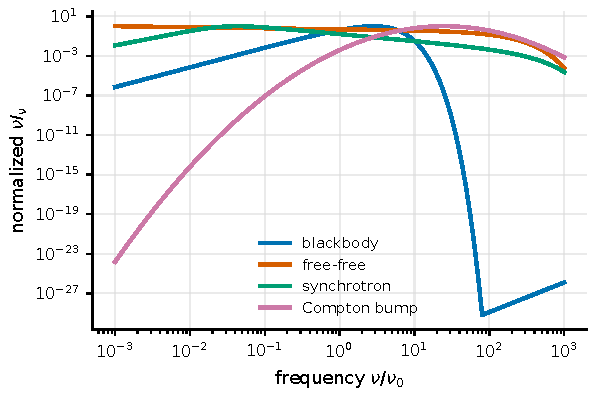
\includegraphics[width=0.84\linewidth]{figures/generated/chapter_09/ch09_spectral_mechanisms.pdf}
\caption{Schematic of the normalized spectral shapes of common continuum radiation mechanisms. A blackbody has a thermal peak and an R--J low-frequency end; free-free radiation is nearly flat in the radio and declines exponentially at high frequency; synchrotron radiation, from a nonthermal electron energy spectrum, gives a power law with low- and high-frequency cutoffs; the inverse-Compton component often appears as a high-energy bump. The four spectral shapes are wildly different, but as long as it is ``many independent particles added together,'' the photon statistics default to the chaotic-thermal-light setting \(g^{(2)}(0)=2\).}
\label{fig:e16-spectral-mechanisms}
\end{figure}

The pedagogical takeaway of this section, in one sentence: \emph{spectrum and polarization can tell you the particle distribution and the field geometry, but they cannot tell you the photon statistics.} Thermal, free-free, synchrotron, inverse-Compton: the spectral shape changes all the way from a thermal peak to a power law to a high-energy bump (Figure~\ref{fig:e16-spectral-mechanisms}), yet they share the same statistical root and are all Gaussian chaotic light. To make \(g^{(2)}\) genuinely deviate from 2, one must break the premise of ``many independent emitters added together,'' and this drives us to the coherent mechanisms of the next section.

\section{Coherent Mechanisms: The Few Exits That Break the Brightness-Temperature Ceiling}
\label{sec:e16-coherent}

To deviate from chaotic thermal light there is only one road: make the emitters no longer independent, let a large number of charges \emph{cooperate} in phase. Once they cooperate, the premise of the central limit theorem collapses, the field is no longer a Gaussian process, the occupation number can shoot up to \(10^{20}\), \(10^{30}\), and the brightness temperature breaks through the incoherent ceiling of \(10^{10}~{\rm K}\). The mechanisms that achieve this in astrophysical sources can be counted on one's fingers, and this section names them one by one.

\paragraph{Stimulated-emission class: masers and lasers.}
\label{sec:e16-maser}

The maser starts from ``negative absorption.'' If a population inversion appears on some spectral line (the upper level more populated than the lower), the absorption coefficient becomes negative, \(\alpha_\nu<0\). Substituted into radiative transfer, the intensity is \emph{exponentially amplified} along the path:
\begin{equation}
  I_\nu(L)\simeq I_\nu(0)\,\exp(|\tau_m|),
  \qquad
  \tau_m=\int_0^L\alpha_\nu\,{\rm d}s<0 .
  \label{eq:e16-maser-gain}
\end{equation}
\begin{formulaexplain}
\(I_\nu(0),I_\nu(L)\) the intensity before and after the path; \(\tau_m<0\) the negative-absorption optical depth. When unsaturated, the gain grows exponentially with \(|\tau_m|\): this is the source of high-brightness-temperature narrow lines.
\end{formulaexplain}
When unsaturated, the gain is exponentially sensitive to the optical depth and can push \(T_b\) extremely high; after saturation, stimulated emission depletes the inversion, and line width, polarization, and intensity are all taken over by the pump and geometry. Water masers, OH masers, and SiO masers can reach extremely high brightness temperatures, and the occupation number is therefore huge. But take care: the coherence of astrophysical masers is usually determined jointly by many velocity-coherent paths, turbulent clumps, and polarization propagation effects, and \emph{cannot} be simply equated with the near-coherent state of a single-mode laser beam in the laboratory. The work of Goldreich, Keeley, Kwan, and Elitzur gives the basic constraints on source size, saturation, line width, and polarization \citep{1972ApJ...174..517G,1973ApJ...179..111G,1974ApJ...190...27G,1982RvMP...54.1225E,1992ARA&A..30...75E}. Stimulated emission is not limited to the radio either: in the Weigelt blobs of Eta Carinae, Fe II and O I lines can, under particular pumping and optical depth, show laser or laser-like amplification, whose line width, position, polarization, and photon correlations can test the inversion and feedback geometry \citep{2004A&A...428..497J,2005NewA...10..361J,2008AIPC..984..216D}. As long as the pumping, level structure, and escape path are suitable, optical spectral lines too can carry statistical signatures distinct from ordinary thermal light.

The electron-cyclotron maser is a coherent radio mechanism in strongly magnetized, low-density plasma. It requires the electron distribution to depart from equilibrium (e.g., a loss-cone distribution), and requires the relation between the cyclotron frequency and the plasma frequency to allow the electromagnetic wave to escape. The cyclotron frequency is
\begin{equation}
  \nu_B=\frac{eB}{2\pi m_ec}
       \simeq2.8~{\rm MHz}\left(\frac{B}{1~{\rm G}}\right).
  \label{eq:e16-cyclotron-frequency}
\end{equation}
\begin{formulaexplain}
\(\nu_B\) the electron-cyclotron frequency; \(e\) the charge, \(B\) the magnetic field, \(m_e\) the electron mass. The observed maser frequency can be used to infer the order of magnitude of the field in the emission region.
\end{formulaexplain}
If one sees the fundamental or a low harmonic of the electron-cyclotron maser at GHz frequency, the field is of order a few hundred G to a few kG. High-circular-polarization radio bursts from the Sun, planets, brown dwarfs, and low-mass stars can all fall into this framework \citep{1982ApJ...259..844M,2006A&ARv..13..229T,2008ApJ...684..644H,1985ARA&A..23..169D}.

\paragraph{Antenna class: coherent curvature radiation.}
\label{sec:e16-curvature}

Curvature radiation demonstrates another road to coherence: it relies not on level inversion but on making many charges move cooperatively in phase, like an antenna. When a relativistic charge moves along a curved magnetic field line, the characteristic frequency and power of a single charge are
\begin{equation}
  \nu_{\rm curv}=\frac{3c}{4\pi\rho}\gamma^3,
  \qquad
  P_{\rm curv}=\frac{2e^2c}{3\rho^2}\gamma^4 ,
  \label{eq:e16-curvature}
\end{equation}
\begin{formulaexplain}
\(\nu_{\rm curv}\) the curvature-radiation characteristic frequency, \(P_{\rm curv}\) the single-particle power; \(\rho\) the radius of curvature of the field line, \(\gamma\) the Lorentz factor. Coherent curvature radiation additionally requires many charges to be phase-synchronized.
\end{formulaexplain}
where \(\rho\) is the radius of curvature of the field line. Plug in numbers: \(\rho=10^7~{\rm cm}\), \(\gamma=300\); compute first the prefactor \(3c/(4\pi\rho)\simeq7.2\times10^2~{\rm Hz}\), then multiply by \(\gamma^3=2.7\times10^7\) to get \(\nu_{\rm curv}\sim2\times10^{10}~{\rm Hz}\) (still in the radio/microwave band). The curvature radiation of a single particle is too weak; coherent curvature radiation requires many charges to bunch on a longitudinal scale smaller than a wavelength, so that the field amplitudes \emph{add} rather than the powers, and the total power grows roughly as the \emph{square} of the particle number. This is the essence of the ``antenna'': if \(N\) charges are phase-synchronized, the radiated power \(\propto N^2\) rather than \(N\). This idea has long been used for pulsar coherent radio emission and has also been carried into FRB models \citep{1977ApJ...212..800C,2018MNRAS.477.2470L}.

FRBs push the coherent mechanism to the extreme. The Lorimer burst provided the first set of evidence for millisecond timescale, cold-plasma dispersion, and \(T_b\sim10^{34}~{\rm K}\); repeaters and the CHIME sample show that repetition, polarization, frequency drift, microstructure, and host environment all enter the models; and the 2020 event from SGR 1935+2154 directly connected a Galactic magnetar to FRB-like radio bursts \citep{2007Sci...318..777L,2019A&ARv..27....4P,2022A&ARv..30....2P,2020Natur.587...54C,2020Natur.587...59B}. The many models fall roughly into two classes: maser-type, relying on population inversion or shocks, and antenna/curvature-type, relying on charge bunches or current sheets. Sub-microsecond structure, strong polarization, frequency drift, and multiband non-detections jointly constrain the emission radius, Lorentz factor, plasma density, and radiation efficiency.

The physical landing point of this section: coherent mechanisms can break the brightness-temperature ceiling and push the occupation number to astronomical numbers because they break the premise of ``independent emitters added together'' and make the charges cooperate. Their photon statistics can \emph{in principle} deviate from chaotic thermal light, but remember, the deviation spoken of here refers to the signature of stimulated/cooperative emission at extremely high occupation numbers, and is not the same as the squeezed, antibunched nonclassical light we pursue in the laboratory. Genuine nonclassical light requires \(g^{(2)}(0)<1\), and in astrophysical sources, even if the source itself has deviated from thermal statistics, whether we can \emph{measure} that deviation must still pass the test of the next section.

\section{Why It Is Extremely Hard to Isolate Genuinely Nonclassical Light in Astrophysical Sources}
\label{sec:e16-dilution}

Now we reach the most crucial, and also the most easily romanticized, point of the chapter. We have said that single-mode thermal light has \(g^{(2)}(0)=2\) and that coherent mechanisms may deviate, which sounds as though one need only set up a detector to read out the mechanism's fingerprint. Real observations, however, almost always \emph{smooth over} these fingerprints. What smooths them is ``mode dilution.''

The physical picture: that beautiful bunching peak of \(g^{(2)}(0)=2\) holds only in a \emph{single} spacetime--polarization mode. But a real telescope collects a great many modes at once: the telescope's receiving aperture covers many spatial coherence patches (spatial modes \(M_{\rm sp}\)), it is sensitive to both polarizations (polarization modes \(M_{\rm pol}\)), and its time resolution \(\Delta t\) is far broader than the coherence time \(\tau_c\) (temporal modes \(\sim\Delta t/\tau_c\)). The fluctuations of these modes are mutually independent, and once averaged, the bunching peak is diluted. Writing out \(M_{\rm eff}\) in the Siegert relation~\eqref{eq:e16-siegert} in detail,
\begin{equation}
  g^{(2)}_{\rm meas}(0)-1\simeq\frac{1}{M_{\rm eff}},
  \qquad
  M_{\rm eff}\simeq M_{\rm sp}\,M_{\rm pol}\left(1+\frac{\Delta t}{\tau_c}\right).
  \label{eq:e16-mode-dilution}
\end{equation}
\begin{formulaexplain}
\(M_{\rm eff}\) the effective number of mixed modes; \(M_{\rm sp},M_{\rm pol}\) the numbers of spatial and polarization modes, \(\Delta t/\tau_c\) the averaging of the time bin over the coherence time. The more modes there are, the lower the measurable bunching contrast \(g^{(2)}_{\rm meas}(0)-1\).
\end{formulaexplain}
where \(M_{\rm sp}\) is the number of mixed spatial modes, \(M_{\rm pol}\) is the number of polarization modes, \(\Delta t\) is the electronic or software time bin, and \(\tau_c\simeq1/\Delta\nu\) is the coherence time set by the spectral bandwidth. Substitute real numbers: for visible light \(\lambda=500~{\rm nm}\) with spectral bandwidth \(\Delta\lambda\simeq1~{\rm nm}\) (here nm is a wavelength unit, labeling \(\Delta\lambda\) rather than the frequency bandwidth), converting to the frequency bandwidth with \(\Delta\nu\simeq c\,\Delta\lambda/\lambda^2\approx1.2\times10^{12}~{\rm Hz}\) gives a coherence time of about \(\tau_c\simeq1/\Delta\nu\sim0.8~{\rm ps}\); a typical electronic time resolution is \(\Delta t\sim100~{\rm ps}\), so \(\Delta t/\tau_c\sim125\). Even with only one spatial and one polarization mode, the bunching peak of single-mode thermal light, which ought to reach 2, is compressed to \(g^{(2)}_{\rm meas}(0)-1\sim1/125\lesssim0.01\), a full two orders of magnitude (Figure~\ref{fig:e16-mode-dilution}). This is why the Hanbury Brown--Twiss intensity interferometry signal is so faint on interstellar scales, why every bit of contrast must be ``fought for'' with narrowband filtering, polarization selection, and spatial-mode control, and why every step of that fight for contrast comes at the cost of photon rate (Chapter~\ref{chap:e10} will settle this account).

\begin{figure}[tbp]
\centering
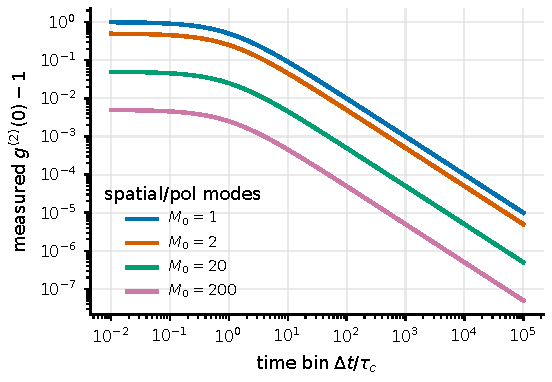
\includegraphics[width=0.82\linewidth]{figures/generated/chapter_09/ch09_thermal_mode_dilution.pdf}
\caption{The thermal-light bunching contrast falls as the effective number of modes rises. The horizontal axis is the ratio of the time bin to the coherence time, and \(M_0\) on the curves represents the number of spatial and polarization modes entering the same correlation estimator. Even if the source itself is pure thermal light, a wide time bin, mixing of multiple polarizations, and mixing of multiple spatial modes all pull \(g^{(2)}(0)-1\) toward zero: this is precisely the fundamental reason why photon-statistics fingerprints are so hard to see in astrophysical sources.}
\label{fig:e16-mode-dilution}
\end{figure}

Now overlay this dilution on the preceding picture and it becomes clear ``why it is extremely hard to isolate genuinely nonclassical light in astrophysical sources.'' First, most mechanisms \emph{by default} give chaotic thermal light (\(g^{(2)}(0)=2\)), and the candidates for nonclassical light (\(g^{(2)}(0)<1\)) can be counted on one's fingers. Second, even if some coherent mechanism in principle deviates from thermal statistics, mode dilution will compress the measurable deviation to \(10^{-2}\) or even lower. Third, even if your signal survives, instrumental and propagation effects will forge spurious correlations: dead time, afterpulsing, timestamp quantization, and trigger selection will rewrite the arrival-time correlation (a spurious \(g^{(2)}\) structure); plasma scintillation, scattering tails, gravitational microlensing, and frequency-dependent absorption will create cross-frequency correlations; a narrow maser line superposed on a thermal background, or a coherent pulse superposed on a synchrotron continuum, will make the mean spectrum look smooth while the photon statistics are no longer of a single kind. So any ``anomalous \(g^{(2)}\) peak'' must first be reconciled item by item against instrument, propagation, and mixed sources before one dares think ``nonclassical'' (Figure~\ref{fig:e16-g2-diagnostics} places the \(g^{(2)}(\tau)\) shapes of single-mode thermal light, multimode dilution, coherent state, and narrow coherent line side by side, precisely the reference figure for this item-by-item screening). The event tables, time-shifted backgrounds, and covariance estimates of Chapters~\ref{chap:e13} and~\ref{chap:e14} provide exactly the analysis layer needed for such item-by-item screening.

\begin{figure}[tbp]
\centering
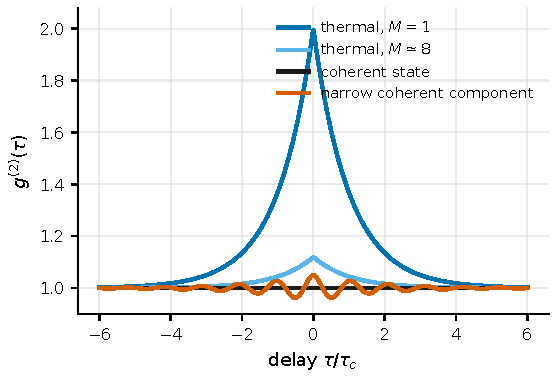
\includegraphics[width=0.82\linewidth]{figures/generated/chapter_09/ch09_radiation_g2_diagnostics.pdf}
\caption{\(g^{(2)}(\tau)\) for different light fields. Single-mode thermal light gives a bunching peak of height 2 at zero delay; multimode averaging lowers the peak (Eq.~\eqref{eq:e16-mode-dilution}); an ideal coherent state approaches 1; a narrow coherent spectral line or stimulated component can leave a small oscillation or narrow peak on a near-Poisson background. The horizontal axis is normalized to the coherence time \(\tau_c\).}
\label{fig:e16-g2-diagnostics}
\end{figure}

The correct posture for mechanism judgment is thus to gather all measurable quantities into the same observation vector for joint diagnosis, rather than staring at the mean spectrum alone:
\begin{equation}
  \bm{d}=
  \left\{
  I_\nu(t),\,
  Q_\nu(t),U_\nu(t),V_\nu(t),\,
  g^{(2)}_{ab}(\tau;\nu_i,\nu_j),\,
  \Delta t_{\rm var},\,
  \Omega_{\rm s}
  \right\}.
  \label{eq:e16-diagnostic-vector}
\end{equation}
\begin{formulaexplain}
\(\bm{d}\) the mechanism-diagnostic observation vector; it simultaneously collects intensity, Stokes polarization, second-order correlation, variability timescale, and angular scale. Mechanism judgment must rely on these quantities \emph{jointly}; the mean spectrum alone is not enough.
\end{formulaexplain}
where \(Q,U,V\) are the Stokes parameters, the subscripts \(a,b\) label telescope, polarization, or frequency channel, \(\Delta t_{\rm var}\) is the variability timescale, and \(\Omega_{\rm s}\) is the angular-scale constraint. Placing each mechanism in this vector separates the fingerprints: a thermal source (low polarization, finite \(T_b\), and residual-after-dilution thermal bunching); optically thin synchrotron (high linear polarization, power-law spectrum); maser (narrow line, extremely high \(T_b\), strong polarization); FRB (extremely high \(T_b\), millisecond-to-microsecond structure, dispersion, strong polarization). And scattering and plasma propagation change the temporal structure and spectrum, yet should \emph{not} be mistaken for the emission statistics of the source itself. Figure~\ref{fig:e16-diagnostic-plane} draws two of these axes (brightness temperature, polarization fraction, with point size indicating the measurable second-order coherence contrast) into a diagnostic plane, helping us locate at a glance which class of mechanism a source roughly falls into.

\begin{figure}[tbp]
\centering
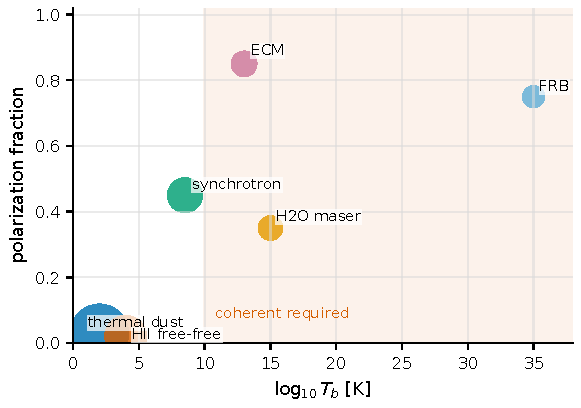
\includegraphics[width=0.86\linewidth]{figures/generated/chapter_09/ch09_diagnostic_plane.pdf}
\caption{The joint diagnostic plane of radiation mechanisms. The horizontal axis is brightness temperature, the vertical axis polarization fraction, and point size indicates the order of magnitude of the measurable second-order coherence contrast. Thermal dust and HII regions sit in the low-brightness-temperature, low-polarization region; synchrotron radiation has higher polarization but a brightness temperature usually below that of coherent bursts; the electron-cyclotron maser, molecular masers, and FRBs enter the high-brightness-temperature region and require coherent emission, pumping, or charge bunching to explain.}
\label{fig:e16-diagnostic-plane}
\end{figure}

\section{Chapter Summary}
\label{sec:e16-summary}

\begin{itemize}
  \item \textbf{The one-sentence main thread.} Translate radiation mechanisms into ``occupation number + photon statistics'': the mean spectrum \(I_\nu\) is only first-order information; the photon-arrival correlation (\(g^{(2)}\)), the polarization correlation, and the cross-frequency joint probability are the true fingerprints of the mechanism.
  \item \textbf{Brightness temperature is the occupation number.} Under the Rayleigh--Jeans definition, \(\bar n_\nu=k_BT_b/(h\nu)\) holds exactly (Eq.~\eqref{eq:e16-occupation-from-tb}). Stellar visible light has \(\bar n_\nu\sim10^{-2}\) (dilute), while an FRB has \(\bar n_\nu\sim10^{36}\) (cooperative). The incoherent-radio brightness-temperature limit is about \(10^{9}\)--\(10^{10}~{\rm K}\); exceeding it requires a coherent mechanism.
  \item \textbf{Thermal and nonthermal both default to chaotic light.} As long as ``many independent emitters add up, with random phase within a narrow band,'' the field is a Gaussian process, and the Siegert relation gives single-mode \(g^{(2)}(0)=2\) (Eq.~\eqref{eq:e16-siegert}). Blackbody, free-free, synchrotron, inverse-Compton: the spectra and polarizations differ, but the photon statistics belong to the same chaotic-thermal-light setting.
  \item \textbf{Only coherent mechanisms may deviate.} Masers/lasers rely on population inversion and stimulated emission; coherent curvature radiation relies on charge bunching (power \(\propto N^2\)). They break the premise of ``independent addition,'' and the occupation number and brightness temperature break through the ceiling, but an astrophysical maser is not the same as a laboratory single-mode laser.
  \item \textbf{Nonclassical light is extremely hard to isolate.} Mode dilution (Eq.~\eqref{eq:e16-mode-dilution}) compresses \(g^{(2)}_{\rm meas}(0)-1\sim1/M_{\rm eff}\) to \(10^{-2}\) or even lower; candidate mechanisms are already scarce; and instrumental and propagation effects can still forge correlations. Mechanism judgment must use the joint diagnostic vector~\eqref{eq:e16-diagnostic-vector} and reconcile the data with the screening tools of Chapters~\ref{chap:e13} and~\ref{chap:e14}.
\end{itemize}

\noindent\textbf{Questions to Ponder.} (1) For a star, the radio end and the optical end have the same matter temperature; why do their occupation numbers \(\bar n_\nu\) differ by several orders of magnitude? (2) The synchrotron spectrum is a power law and its polarization can reach 70\%; on what grounds do we say its photon statistics belong to the same setting as a blackbody? (3) If you see \(g^{(2)}(0)=1.01\) in the data, what are at least three classes of spurious signal you must rule out before concluding ``bunching detected''?

\chapter{Stars as Quantum Light Sources}
\label{chap:e17}

\begin{chapteropening}
In the previous chapter we translated the various astrophysical radiation mechanisms into quantum language: blackbody, thermal light, and stimulated emission each correspond to particular photon statistics. Now let us point this language at the most ordinary, and most reliable, class of source in the night sky: stars. Their photospheres approximate a surface glowing with thermal light, their angular diameters fall in the milliarcsecond (mas) range, and bright stars deliver enough photons per second to make correlation measurements feasible. Better still, intensity interferometry measures only the correlation of the intensity fluctuations of two telescopes, reading out \(|V|^2\) directly, and requires no optical phase to be maintained between them. This chapter answers one question: when we treat a star no longer as a point but as a glowing surface with structure, what distinct, resolvable fingerprint does each of limb darkening, rapid rotation, circumstellar disks, binarity, and pulsation carve into the \(|V(B)|^2\) curve? Along the way we will recycle the van Cittert--Zernike theorem and the uniform disk of Chapter~\ref{chap:e10}, together with the angular diameter and multi-baseline imaging of Chapter~\ref{chap:e11}, and bring them to bear on VERITAS observations of real stars such as \(\beta\) UMa and \(\gamma\) Cas \citep{1956Natur.177...27B,1974MNRAS.167..121H,1974iiia.book.....H,2020NatAs...4.1164A,2024MNRAS.529.4387A}.
\end{chapteropening}

\section{Why Stars Are the Most Stable Calibration Field}
\label{sec:e17-why-stars}

Start with an intuition: to check whether a ruler is accurate, you measure something whose size you roughly know and that will not move around. Stars are just such an ideal calibrator for the new ruler of quantum astronomy. Under local thermodynamic equilibrium (LTE), the photosphere emits a near-blackbody continuum whose spectral shape and total flux can be described by mature stellar-atmosphere models; bright stars are bright enough that the photon-statistics error can be beaten down by integration time; and their angular diameters fall precisely in the window resolvable by hundred-meter baselines in the visible. Chapter~\ref{chap:e16} already explained that such thermal light satisfies \(g^{(2)}(0)=2\) in a single coherent mode: photons arrive in clumps, with fluctuations twice those of a coherent state.

But the \(g^{(2)}(0)-1\) seen by a real telescope is far smaller than 1. The reason is mode dilution: a single measurement mixes in a large number of spatial, polarization, frequency, and temporal modes, each contributing an independent thermal fluctuation, and the contrast is lowered by the averaging. The quantitative statement given in Chapter~\ref{chap:e08} is the dilution factor \(\zeta\) in the Siegert relation, roughly equal to ``the spacetime volume occupied by a single coherent mode divided by the spacetime volume actually received by the detector.'' On a star, this is not an abstract proposition: a photon-counting intensity interferometry experiment on Vega measured \(\langle g^{(2)}\rangle=1.0034\pm0.0008\) at zero baseline, higher than 1 by only three parts per thousand; on a baseline of about \(2~{\rm km}\) no significant correlation could be measured, fully consistent with Vega's angular diameter of about \(3.3~{\rm mas}\): the star is too large, a kilometer baseline has long resolved it out, and the visibility drops to near zero \citep{2021MNRAS.506.1585Z}. This is what the mode dilution of Chapter~\ref{chap:e08} looks like on a real star.

\paragraph{Intensity correlation directly gives the squared visibility.}
\label{sec:e17-g2-vis}

Intensity interferometry measures the zero-delay correlation of the intensity fluctuations of two telescopes. For thermal light, after subtracting background and applying time-shift normalization, the excess of this correlation is proportional to the squared modulus of one Fourier mode of the sky brightness distribution:
\begin{equation}
  g^{(2)}_{ij}(0)-1 \;=\; |\gamma_{ij}|^2 \;\simeq\; \bigl|V(u_{ij},v_{ij})\bigr|^2 .
  \label{eq:e17-g2-vis}
\end{equation}
\begin{formulaexplain}
\(g^{(2)}_{ij}(0)\): the zero-delay intensity correlation of telescopes \(i,j\). \(\gamma_{ij}\): the complex degree of coherence between the two telescopes. \(V\): the normalized complex visibility, with \((u,v)\) the projected baseline divided by wavelength. This equation says: the excess intensity correlation of thermal light is the squared modulus of a Fourier mode of the sky brightness.
\end{formulaexplain}
Let us account for the symbols one by one. \(g^{(2)}_{ij}(0)\) is dimensionless, the result of multiplying the two photocurrents (or photon counts) at the same instant and normalizing by their respective means; Chapter~\ref{chap:e08} already derived that it is 2 for thermal light and 1 for a coherent state. \(\gamma_{ij}\) is the complex degree of coherence, with modulus between 0 and 1; \((u,v)=\bm{B}_\perp/\lambda\) is the spatial frequency obtained by dividing the projected baseline \(\bm{B}_\perp\) (in cm) by the wavelength \(\lambda\) (in cm), with units of ``wavelengths per radian,'' that is, the number of fringes per radian. The left side of~\eqref{eq:e17-g2-vis} comes from real data processing: delay histogram, time-shift background subtraction, normalized correlation; the right side is the purely geometric Fourier transform of the sky brightness. The crux is that the right side is taken as a squared modulus, so the complex phase is entirely lost. This means \(|V|^2\) is insensitive to overall translation and mirror flip of the sky image (translation only changes the Fourier phase, a mirror takes the complex conjugate, and the squared modulus sees neither). But as long as the target structure itself has a definite geometry (the diameter of a disk, the axis ratio of an ellipse, the separation of a binary pair), these quantities can still be read precisely from \(|V|^2\). This is exactly what every subsequent section of this chapter sets out to do.

\paragraph{Baseline length and angular scale are the same ruler.}
\label{sec:e17-baseline}

To resolve a structure of angular scale \(\theta\), how long a baseline is needed? The answer comes from the most elementary dimensional relation in the van Cittert--Zernike theorem:
\begin{equation}
  B \;\sim\; \frac{\lambda}{\theta}
  \;\simeq\; 103~{\rm m}
  \left(\frac{\lambda}{500~{\rm nm}}\right)
  \left(\frac{\theta}{1~{\rm mas}}\right)^{-1}.
  \label{eq:e17-baseline}
\end{equation}
\begin{formulaexplain}
\(B\): the required baseline length. \(\lambda\): the observing wavelength. \(\theta\): the target angular scale. In the visible, a milliarcsecond star corresponds to a hundred-meter baseline, and kilometer baselines are needed to reach sub-milliarcsecond surface detail.
\end{formulaexplain}
Only by working out this order of magnitude for yourself do you truly understand it. Take \(\lambda=500~{\rm nm}=5\times10^{-7}~{\rm m}\) and \(\theta=1~{\rm mas}\). Converting 1 mas to radians requires multiplying by \(4.848\times10^{-9}\) (because \(1~{\rm arcsec}=1/206265~{\rm rad}\), then dividing by 1000), i.e., \(\theta=4.848\times10^{-9}~{\rm rad}\). Hence
\[
  B\sim\frac{\lambda}{\theta}=\frac{5\times10^{-7}~{\rm m}}{4.848\times10^{-9}}
  \approx 103~{\rm m}.
\]
This is the origin of the coefficient 103 m in~\eqref{eq:e17-baseline}. It tells us that a \(1~{\rm mas}\) star begins to be clearly resolved only with a hundred-meter baseline in the visible; while \(0.1~{\rm mas}\) surface structure (such as rotational oblateness or starspots) requires kilometer-scale baselines. Historically the Narrabri intensity interferometer used variable baselines of \(10\)--\(188~{\rm m}\) and two \(6.7~{\rm m}\) reflectors to measure the angular diameters of 32 bright stars \citep{1974MNRAS.167..121H,1974iiia.book.....H}. Today VERITAS, MAGIC, and the future CTA-class arrays, with Cherenkov telescopes of \(>10~{\rm m}\) aperture, larger light-collecting area, and digital correlators, have reopened this parameter space \citep{2020NatAs...4.1164A,2024MNRAS.529.4387A}.

The scaling of the signal-to-noise ratio was given in full in Eq.~\eqref{eq:e11-snr} of Chapter~\ref{chap:e11}; here we only name its direct implication for stellar target selection: the higher the photon rate, the larger the electronic bandwidth, and the longer the integration, the smaller the error on \(|V|^2\) (the signal-to-noise ratio grows only as the square root of integration time); while background light, detector dead time, finite time resolution, and systematic covariance determine where this statistical gain ceases to ``pay off.'' So the first targets naturally lean toward bright, hot, blue stars whose angular diameters are already resolvable at hundred-meter baselines \citep{2013MNRAS.430.3187R,2020NatAs...4.1164A}. This is not a slogan; it is the physical basis for the ``how to lay out baselines'' of the next section.

\section{Reading Angular Diameter and Temperature from the Squared Visibility}
\label{sec:e17-diameter-teff}

The first step from data to radius is to treat the star, provisionally, as a ``uniformly glowing coin,'' with a single parameter: the angular diameter \(\theta\). This is the uniform disk model of Chapter~\ref{chap:e10}, whose visibility is given by Eq.~\eqref{eq:e10-disk},
\[
  V_{\rm UD}(B)=\frac{2J_1(x)}{x},\qquad x=\frac{\pi\theta B}{\lambda},
\]
where \(J_1\) is the first-order Bessel function and \(x\) is the dimensionless ``degree of resolution.'' Here \(B\) is the projected baseline, \(\lambda\) is the effective wavelength, and \(\theta\) must be in radians (if given in mas, multiply by \(4.848\times10^{-9}\)). Intensity interferometry fits \(|V_{\rm UD}|^2\), the complex phase already erased by the squared modulus. The most information-dense place on the curve is near the first null (\(x=3.8317\), corresponding to \(B_0\approx1.22\lambda/\theta\)): there \(|V|^2\) is most sensitive to the angular diameter; but near the null \(|V|^2\) is so small that background and systematic errors can swamp the signal. So a real measurement must cover short, intermediate, and long baseline segments: short baselines fix the total flux and the correlation normalization, intermediate baselines give the falling slope that yields the diameter, and long baselines test whether the model still needs limb darkening, oblateness, or a companion.

\begin{figure}[tbp]
\centering
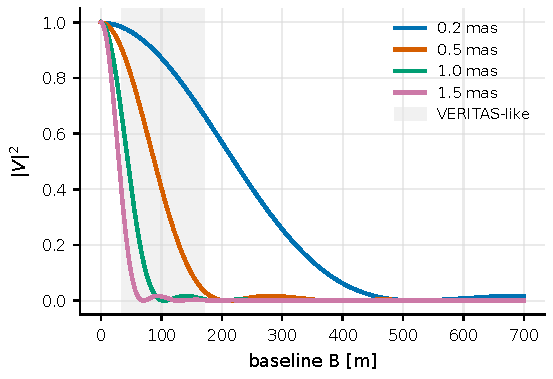
\includegraphics[width=0.82\linewidth]{figures/generated/chapter_10/ch10_stellar_diameter_visibility.pdf}
\caption{The \(|V|^2\) of a uniform-disk star versus baseline. The wavelength is taken as \(416~{\rm nm}\), close to the observing wavelength of VERITAS intensity interferometry. The larger the angular diameter, the faster the visibility falls; the gray region marks the VERITAS-scale projected-baseline range of \(35\)--\(170~{\rm m}\), suited to measuring bright stars of about \(0.5\)--\(1.5~{\rm mas}\).}
\label{fig:e17-diameter-visibility}
\end{figure}

\paragraph{Angular diameter plus total flux equals effective temperature.}
\label{sec:e17-teff}

Once the angular diameter is measured, knowing this star's total radiant flux at Earth is all it takes to obtain its effective temperature. The derivation needs only the Stefan--Boltzmann law plus one step of geometry. The stellar luminosity is \(L=4\pi R^2\sigma_{\rm SB}T_{\rm eff}^4\), where \(R\) is the radius. Propagated to distance \(d\), the bolometric flux received at Earth is \(F_{\rm bol}=L/(4\pi d^2)=R^2\sigma_{\rm SB}T_{\rm eff}^4/d^2\). And the relation between angular diameter and radius is \(\theta_{\rm LD}=2R/d\), i.e., \(R/d=\theta_{\rm LD}/2\), so \(R^2/d^2=\theta_{\rm LD}^2/4\). Substituting back, the distance \(d\) cancels automatically:
\begin{equation}
  F_{\rm bol}=\frac{\theta_{\rm LD}^2}{4}\,\sigma_{\rm SB}T_{\rm eff}^4,
  \qquad
  T_{\rm eff}=\left(\frac{4F_{\rm bol}}{\sigma_{\rm SB}\theta_{\rm LD}^2}\right)^{1/4}.
  \label{eq:e17-teff}
\end{equation}
\begin{formulaexplain}
\(F_{\rm bol}\): the total radiant flux measured at Earth (\({\rm erg\,s^{-1}\,cm^{-2}}\)). \(\theta_{\rm LD}\): the limb-darkened angular diameter. \(\sigma_{\rm SB}\): the Stefan--Boltzmann constant. Angular diameter and total flux together fix the effective temperature without any need to know the distance.
\end{formulaexplain}
Note the beautiful feature: the distance \(d\) is cancelled out in the derivation, so \(T_{\rm eff}\) is a quantity ``independent of the distance scale'': you need only measure the angular diameter and the flux. The subscript LD on \(\theta_{\rm LD}\) reminds us that the limb-darkened angular diameter should be used here (the next section explains why the uniform-disk diameter cannot), in radians or mas; \(\sigma_{\rm SB}=5.67\times10^{-5}~{\rm erg\,s^{-1}\,cm^{-2}\,K^{-4}}\) (CGS).

For the same star, we care more about how the measurement error propagates to \(T_{\rm eff}\). Since \(T_{\rm eff}\propto F_{\rm bol}^{1/4}\theta_{\rm LD}^{-1/2}\), taking logarithms gives \(\ln T_{\rm eff}=\tfrac14\ln F_{\rm bol}-\tfrac12\ln\theta_{\rm LD}+{\rm const}\). Differentiating: \({\rm d}\ln T_{\rm eff}=\tfrac14\,{\rm d}\ln F_{\rm bol}-\tfrac12\,{\rm d}\ln\theta_{\rm LD}\). If the errors of \(F_{\rm bol}\) and \(\theta_{\rm LD}\) are independent, the variances add in quadrature and the coefficients are squared:
\begin{equation}
  \left(\frac{\sigma_T}{T_{\rm eff}}\right)^2
  \simeq
  \frac{1}{16}\left(\frac{\sigma_F}{F_{\rm bol}}\right)^2
  +\frac{1}{4}\left(\frac{\sigma_\theta}{\theta_{\rm LD}}\right)^2 .
  \label{eq:e17-teff-error}
\end{equation}
\begin{formulaexplain}
\(\sigma_T,\sigma_F,\sigma_\theta\): the absolute errors of temperature, total flux, and angular diameter. Because \(T_{\rm eff}\propto F_{\rm bol}^{1/4}\theta_{\rm LD}^{-1/2}\), for the same percentage error the angular-diameter term (coefficient \(1/4\)) carries four times the weight of the flux term (coefficient \(1/16\)).
\end{formulaexplain}
The coefficients \(1/16=(1/4)^2\) and \(1/4=(1/2)^2\) are precisely the squares of the exponents. The conclusion: the relative error of the angular diameter enters \(T_{\rm eff}\) with four times the weight of the flux, so the angular diameter often dominates the temperature precision. This is exactly the value of intensity interferometry: it turns an angular diameter that was once inferred indirectly through models into a direct measurement. VERITAS intensity-interferometry observations of \(\beta\) Ursae Majoris (\(\beta\) UMa) gave \(\theta_{\rm LD}=1.07\pm0.04\,({\rm stat})\pm0.05\,({\rm sys})~{\rm mas}\), which substituted into~\eqref{eq:e17-teff} yields \(T_{\rm eff}\simeq9700\pm200\pm200~{\rm K}\), and can further constrain the age of the Ursa Major moving group \citep{2024ApJ...966...28A}. And the two bright blue stars \(\beta\) Canis Majoris (\(\beta\) CMa) and \(\epsilon\) Orionis (\(\epsilon\) Ori), measured in the first modern VERITAS intensity-interferometry survey, are exactly the opening act of this method in the real sky \citep{2020NatAs...4.1164A}.

\begin{figure}[tbp]
\centering
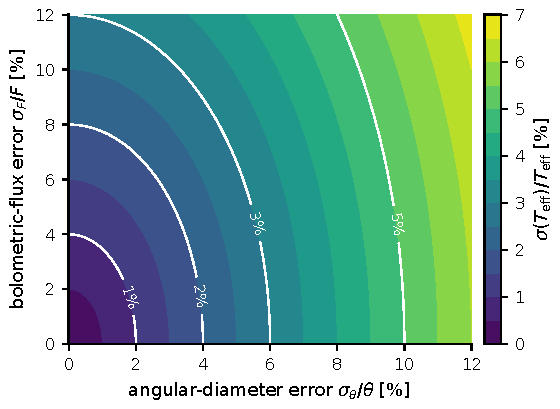
\includegraphics[width=0.78\linewidth]{figures/generated/chapter_10/ch10_teff_error_budget.pdf}
\caption{Error propagation for deriving \(T_{\rm eff}\) from \(F_{\rm bol}\) and \(\theta_{\rm LD}\). The horizontal axis is the relative error of the angular diameter, the vertical axis the relative error of the total flux, and color gives the relative error of the effective temperature. Because \(T_{\rm eff}\propto F_{\rm bol}^{1/4}\theta_{\rm LD}^{-1/2}\), an angular-diameter error is usually more ``valuable'' than a flux error of the same percentage.}
\label{fig:e17-teff-error}
\end{figure}

\paragraph{Add the distance to get radius and luminosity.}
\label{sec:e17-radius}

If this star's distance \(d\) is given independently by the Gaia parallax, then the angular diameter can be translated into a physical radius, and the Stefan--Boltzmann law then gives the luminosity:
\begin{equation}
  R=\frac{1}{2}\theta_{\rm LD}\,d,\qquad
  L=4\pi R^2\sigma_{\rm SB}T_{\rm eff}^4 .
  \label{eq:e17-radius}
\end{equation}
\begin{formulaexplain}
\(R\): the physical stellar radius. \(d\): the distance. \(L\): the luminosity. The angular diameter gives ``how large on the sky,'' the distance turns it into ``how large in reality,'' and the Stefan--Boltzmann law then gives ``how bright it shines.''
\end{formulaexplain}
The first equation is just a rewriting of \(\theta_{\rm LD}=2R/d\); \(\theta_{\rm LD}\) is in radians, and \(d\) and \(R\) are in the same unit (both cm, say, or if \(d\) is in pc and \(R\) in \(R_\odot\), remember to convert). Combining the Gaia parallax, the intensity-interferometry angular diameter, and \(F_{\rm bol}\), a star falls into a small region with covariance on the Hertzsprung--Russell (HR) diagram. Comparing this small region with stellar evolutionary tracks constrains the mass, age, and model parameters such as the mixing length, convective overshoot, and rotation. The infrared flux method, the angular diameters from amplitude interferometers such as Mark III and CHARA, and the intensity-interferometry angular diameters are, at this level, mutually corroborating independent rulers \citep{1977MNRAS.180..177B,1991AJ....101.2207M,1994A&A...282..899B,2003AJ....126.2502M,2005ApJ...626..446R}.

\section{Why Limb Darkening Is Not a Small Correction}
\label{sec:e17-limb-darkening}

Treating the star as a uniform coin incurs a debt that must be repaid: the edge of a real stellar disk is darker. The reason is very physical: when you look toward the disk center, the line of sight plunges vertically into the atmosphere and sees the deeper, hotter layers; when you look toward the edge, the line of sight grazes at a steep angle and sees only the shallower, cooler upper layers. Lower temperature means lower brightness, so the edge grows dark; this is limb darkening. The simplest linear model is
\begin{equation}
  I(\mu)=I(1)\,[1-u_\lambda(1-\mu)],
  \qquad
  \mu=\sqrt{1-r^2}.
  \label{eq:e17-linear-ld}
\end{equation}
\begin{formulaexplain}
\(I(\mu)\): the surface brightness at different viewing angles. \(\mu\): the cosine of the angle between the surface normal and the line of sight. \(r\): the normalized projected radius (center \(r=0\), edge \(r=1\)). \(u_\lambda\): the wavelength-dependent limb-darkening coefficient. It compresses ``the edge darkens'' into a single parameter.
\end{formulaexplain}
Term by term: \(r\) is the radius on the projected disk divided by the stellar radius, ranging from 0 to 1; at the center the line of sight is perpendicular and \(\mu=1\), at the edge it grazes and \(\mu=0\), the geometric relation being precisely \(\mu=\sqrt{1-r^2}\). \(I(1)\) is the central brightness. \(u_\lambda\) is the limb-darkening coefficient: \(u_\lambda=0\) reverts to the uniform disk, and the larger \(u_\lambda\), the darker the edge; it is dimensionless and depends strongly on wavelength: for a hot star in the blue, a cool giant in a molecular absorption band, or a Mira variable at different pulsation phases, \(u_\lambda\) all differ. Modern analyses usually do not use this linear form but instead generate a synthetic \(I(\mu)\) directly from an atmosphere model and then compute the visibility; the linear \(u_\lambda\) is used mainly for order-of-magnitude estimates and intuition \citep{1974MNRAS.167..475H,1992A&A...259..227D,1997A&A...327..199H,2015MNRAS.453.3821P}.

\paragraph{The visibility of any radial profile is a Hankel transform.}
\label{sec:e17-hankel}

To learn how limb darkening changes the visibility curve, we need a formula that can accept ``any radial brightness profile.'' For any axisymmetric (circularly symmetric) brightness distribution \(I(r)\), its visibility is the radial Hankel transform:
\begin{equation}
  V(x)=
  \frac{\displaystyle\int_0^1 I(r)\,J_0(xr)\,r\,{\rm d}r}
       {\displaystyle\int_0^1 I(r)\,r\,{\rm d}r},
  \label{eq:e17-hankel}
\end{equation}
\begin{formulaexplain}
\(V(x)\): the visibility of an axisymmetric brightness distribution. \(J_0\): the zeroth-order Bessel function. \(x\): the dimensionless spatial frequency assembled from baseline, wavelength, and angular radius. The denominator is the normalization (total flux), and the numerator projects the brightness profile onto that frequency.
\end{formulaexplain}
Where does this equation come from? When a two-dimensional Fourier transform acts on a circularly symmetric function, the azimuthal integral \(\int_0^{2\pi}e^{-i x r\cos\phi}\,{\rm d}\phi=2\pi J_0(xr)\): this is the integral representation of the zeroth-order Bessel function, a standard result, which reduces the two-dimensional Fourier transform directly to a one-dimensional radial integral. The denominator \(\int_0^1 I(r)\,r\,{\rm d}r\) is the total flux, ensuring \(V(0)=1\). The uniform disk is the special case \(I(r)={\rm const}\): here the numerator uses another standard result \(\int_0^1 J_0(xr)\,r\,{\rm d}r=J_1(x)/x\), the denominator is \(1/2\), and dividing one by the other returns exactly to \(V=2J_1(x)/x\), i.e., Eq.~\eqref{eq:e10-disk}. Substituting the linear profile with \(u_\lambda>0\), the darkened edge makes the disk boundary no longer ``sharp,'' with the effect of pushing the first null of the visibility outward and lowering the height of the first sidelobe.

\begin{figure}[tbp]
\centering
\includegraphics[width=0.92\linewidth]{figures/generated/chapter_10/ch10_limb_darkening.pdf}
\caption{The effect of linear limb darkening on surface brightness and visibility. The left panel shows the radial brightness profile for the three cases \(u_\lambda=0,0.4,0.8\); the right panel shows the corresponding \(|V|^2\) obtained by numerically integrating Eq.~\eqref{eq:e17-hankel}. The darker the edge, the more blurred the disk boundary, and the positions of the visibility nulls and sidelobes shift accordingly.}
\label{fig:e17-limb-darkening}
\end{figure}

This is precisely why limb darkening is not a ``drawing detail'' but a source of systematic error: for the same set of \(|V|^2\) data, fitting with a uniform disk gives \(\theta_{\rm UD}\), while fitting with a limb-darkened atmosphere model gives \(\theta_{\rm LD}\), closer to the true photospheric boundary, and the two can differ by a few percent. What it changes is not whether the curve looks nice but ``which radius you are actually measuring.'' Back then, the Narrabri angular-diameter catalog had to correct the uniform-disk diameter into a limb-darkened diameter before temperature and radius could be discussed further \citep{1974MNRAS.167..121H,1974MNRAS.167..475H}. For intensity interferometry, the calibration error must further stack together the effects of the catalog angular diameter, correlator gain, time synchronization, background light, and \(|V|^2\) covariance; each item must be accounted for separately.

\section{How Rotation, Binarity, and Surface Structure Enter the Visibility}
\label{sec:e17-rotation-binary}

So far the star has still been a circle. In reality it may be flattened by rotation, may have a companion, may be mottled on its surface. These structures write non-circular, non-symmetric information into \(|V|^2\), and we examine what each fingerprint looks like in turn.

\paragraph{Rapid rotation: oblateness and gravity darkening.}
\label{sec:e17-rotation}

A rapidly rotating star has its equator flung outward by centrifugal force, and the photosphere goes from a sphere to an oblate spheroid. More subtly, there is gravity darkening: with the equator bulged out, the surface gravity there decreases, and so does the surface temperature there, so the equator is darker and cooler than the poles. The first geometric effect is that the projection is an ellipse. Approximating the projected photosphere as an ellipse, the effective angular diameter seen along the baseline direction \(\psi\) is
\begin{equation}
  \theta_{\rm eff}^2(\psi)=
  \theta_{\rm maj}^2\cos^2\psi+
  \theta_{\rm min}^2\sin^2\psi ,
  \label{eq:e17-ellipse}
\end{equation}
\begin{formulaexplain}
\(\theta_{\rm eff}(\psi)\): the effective angular diameter seen along the baseline direction \(\psi\). \(\theta_{\rm maj},\theta_{\rm min}\): the major- and minor-axis angular diameters of the projected ellipse. Rotational oblateness makes the falling rate of \(|V|^2\) vary with position angle.
\end{formulaexplain}
This equation is just the ``apparent width'' formula for an ellipse in direction \(\psi\): when the baseline is along the major axis (\(\psi=0\)) then \(\theta_{\rm eff}=\theta_{\rm maj}\), the star looks ``widest'' and the visibility falls fastest; along the minor axis (\(\psi=90^\circ\)) then \(\theta_{\rm eff}=\theta_{\rm min}\), and the visibility falls slowest. So a baseline of the same length, pointed at different position angles, reads different \(|V|^2\): this is the resolvable fingerprint left by oblateness. This is exactly how VERITAS intensity-interferometry observations of \(\gamma\) Cassiopeiae (\(\gamma\) Cas) at \(416~{\rm nm}\) measured the oblateness: minor-axis angular diameter \(0.43\pm0.02~{\rm mas}\), major-to-minor radius ratio \(1.28\pm0.04\), position angle \(116^\circ\pm5^\circ\); then using a rapid-rotation atmosphere model, they further gave a lower bound on the rotation velocity close to breakup and an equatorial radius of about \(10.9~R_\odot\) \citep{2025ApJ...995..191A}.

\begin{figure}[tbp]
\centering
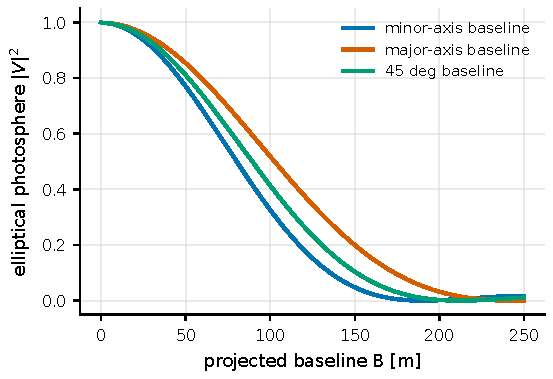
\includegraphics[width=0.82\linewidth]{figures/generated/chapter_10/ch10_rotation_oblateness.pdf}
\caption{The \(|V|^2\) of a rapidly rotating elliptical photosphere along different baseline directions. Parameters are taken at the \(\gamma\) Cas-scale axis ratio of \(1.28\) and \(416~{\rm nm}\) wavelength. Projected along different position angles, the effective angular diameter differs, so the same baseline length gives a different correlation strength; this geometric effect lets intensity interferometry measure the photospheric oblateness directly.}
\label{fig:e17-rotation}
\end{figure}

\paragraph{Binaries: cosine oscillations in visibility space.}
\label{sec:e17-binary}

A pair of close binary stars, neither yet resolved individually, overlays a layer of cosine ripples on the visibility curve. The derivation is direct: treat the two stars as two point sources, the primary flux taken as 1, the secondary as \(f\) (the flux ratio), with angular separation vector \(\bm{d}\). The visibility of two point sources is the weighted sum of their complex phases, \(V=(1+f\,e^{i\phi})/(1+f)\), where the phase \(\phi=2\pi\bm{u}\cdot\bm{d}\) comes from the optical path difference of the two point sources. Taking the squared modulus: \(|1+f e^{i\phi}|^2=(1+f\cos\phi)^2+(f\sin\phi)^2=1+f^2+2f\cos\phi\). Dividing by the normalization \((1+f)^2\):
\begin{equation}
  |V_{\rm bin}|^2=
  \frac{1+f^2+2f\cos(2\pi\bm{u}\cdot\bm{d})}
       {(1+f)^2}.
  \label{eq:e17-binary}
\end{equation}
\begin{formulaexplain}
\(|V_{\rm bin}|^2\): the squared visibility of an unresolved binary. \(f\): the flux ratio of secondary to primary. \(\bm{u}=\bm{B}_\perp/\lambda\): the spatial frequency. \(\bm{d}\): the angular separation vector (radians). The cosine term makes the binary oscillate in baseline space.
\end{formulaexplain}
Reading this equation: the oscillation period is set by \(\bm{u}\cdot\bm{d}\): the larger the separation \(\bm{d}\) and the longer its projection along the baseline, the faster it oscillates with baseline, so the angular separation along the baseline direction can be inferred from the oscillation period; the depth of the oscillation is set by \(f\), and when \(f\to1\) (two equally bright stars) the coefficient of the cosine term \(2f/(1+f)^2\to1/2\) is maximal and the ripples are deepest, while for \(f\to0\) (a very faint secondary) the ripples vanish. If the two stars are each partially resolved, one need only multiply each term by its own disk visibility, Eq.~\eqref{eq:e10-disk}. Some targets in the Narrabri catalog were later recognized as binaries or multiples; modern multi-baseline intensity-interferometry arrays can jointly fit the binary orbit, angular diameters, and brightness ratio, and combined with radial velocities determine the masses \citep{1970MNRAS.148..103H,1974MNRAS.167..121H,2012MNRAS.419..172N}.

\begin{figure}[tbp]
\centering
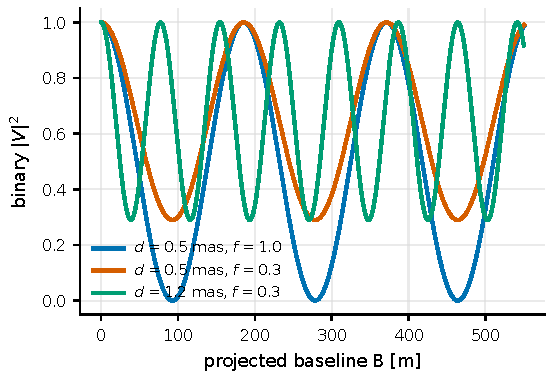
\includegraphics[width=0.82\linewidth]{figures/generated/chapter_10/ch10_binary_visibility.pdf}
\caption{The \(|V|^2\) oscillation of an unresolved binary. The larger the angular separation, the faster the oscillation with baseline; the closer the flux ratio to 1, the larger the oscillation amplitude. A real binary further requires the finite angular diameters of the two stars, the orbital position angle, and the multi-wavelength flux ratio.}
\label{fig:e17-binary}
\end{figure}

\paragraph{Surface structure: the degeneracy brought by missing phase.}
\label{sec:e17-surface}

Surface structure is thornier than binarity, because \(|V|^2\) lacks phase. Starspots, large convective granules, non-radial pulsations, and Be-star disks all introduce non-axisymmetric signals; if one merely fits a disk or binary model, one may well get a result that ``fits the curve beautifully but is physically wrong,'' exactly the model degeneracy caused by missing phase. The way to break it is to add dimensions of constraint: multiple baselines, multiple nights, multiple wavelengths, and spectral-line channels can each suppress part of the degeneracy. Simulation studies show that a Cherenkov telescope array, with enough baseline number and coverage, has a chance to reconstruct diameter, oblateness, binary structure, and even large-scale surface features; but to reconstruct a genuinely complex image still requires prior information or joint use with amplitude-interferometry data \citep{2012MNRAS.419..172N,2013MNRAS.430.3187R}.

\section{How Time Variation and Spectral-Line Channels Extend the Stellar Image}
\label{sec:e17-time-line}

The stars so far have all been ``static.'' The final section lets stars move and lets different wavelengths speak for themselves, to see what more intensity interferometry can measure.

\paragraph{Cepheids: connecting the angular-radius change to the distance scale.}
\label{sec:e17-cepheid}

A Cepheid variable periodically swells and shrinks, and its angular diameter changes with pulsation phase. This gives a ruler for the heavens independent of parallax: the Baade--Wesselink class of methods. The idea is: the radial-velocity spectral lines tell us the surface velocity along the line of sight, and integrating it gives the physical change in radius \(\Delta R\); while intensity interferometry directly measures the change in angular radius \(\Delta\theta\). The ratio of the two is the distance. Quantitatively, first fix conventions: the radial velocity \(v_r\) is positive away from us (redshift positive), and when the surface expands toward us the line is blueshifted, \(v_r-v_\gamma<0\), while the radius is then increasing, so the rate of change of radius and the radial pulsation velocity differ by a minus sign,
\[
  \frac{{\rm d}R}{{\rm d}t}=-p\,[v_r(t)-v_\gamma].
\]
Integrating both sides over time gives the physical change in radius
\[
  \Delta R(t)=-\int p\,[v_r(t)-v_\gamma]\,{\rm d}t.
\]
Using the geometric relation between angular diameter and radius \(\Delta\theta=2\Delta R/d\) and substituting gives
\begin{equation}
  \Delta\theta(t)=-\frac{2}{d}
  \int p\,[v_r(t)-v_\gamma]\,{\rm d}t .
  \label{eq:e17-baade-wesselink}
\end{equation}
\begin{formulaexplain}
\(\Delta\theta(t)\): the change of angular diameter with time. \(d\): the distance. \(v_r-v_\gamma\): the radial pulsation velocity after subtracting the overall systemic velocity (positive away). \(p\): the projection factor converting the observed radial velocity into the true pulsation velocity. The minus sign is a consequence of the velocity sign convention; the actual analysis cares only about the amplitude and phase of \(\Delta\theta(t)\), the sign fixed by convention.
\end{formulaexplain}
Term by term: \(v_r(t)\) is the radial velocity measured from the spectral lines, \(v_\gamma\) is the systemic velocity of the whole star relative to us (a constant), and it is their difference that is the pulsation itself. The minus sign in the equation comes purely from the sign convention ``radial velocity positive away, while expansion brings the surface toward us''; switch conventions and the sign flips, and in a real distance fit only the shape (amplitude and phase) of the \(\Delta\theta(t)\) curve is used, so the sign does not affect the result, but getting it right keeps the main-text derivation and the boxed formula internally consistent. \(p\) is the projection factor, because a spectral line is a radial-velocity-weighted average over the whole visible hemisphere, whereas what we want is the true radial expansion velocity of the surface, the two differing by a geometric factor of order \(1.3\). Once the angular-diameter curve \(\Delta\theta(t)\) is phase-matched to the velocity-integral curve, the only free scale left is \(d\), and the distance is thereby fixed. The systematic errors come from the \(p\)-factor, limb darkening (\(u_\lambda\) changes during pulsation), companion contamination, period changes, and atmospheric velocity gradients. Bright Cepheids are especially tempting for visible-light intensity interferometry: they are both bright and have a predictable radius change \citep{1997A&A...320..799F,2007A&A...476...73F}.

\paragraph{Spectral-line channels: separating the structure of the continuum and line regions.}
\label{sec:e17-line}

For Be stars and Wolf--Rayet stars, the continuum comes from the photosphere while the emission lines come from an extended disk or wind, the two on different spatial scales. If a narrowband filter frames the continuum and an emission line at once, the observed visibility is the flux-weighted sum of the two:
\begin{equation}
  V_{\rm obs}=
  \frac{F_{\rm cont}V_{\rm cont}+F_{\rm line}V_{\rm line}}
       {F_{\rm cont}+F_{\rm line}} .
  \label{eq:e17-line-visibility}
\end{equation}
\begin{formulaexplain}
\(V_{\rm obs}\): the net visibility observed within the narrow band. \(F_{\rm cont},F_{\rm line}\): the fluxes of the continuum and the line. \(V_{\rm cont},V_{\rm line}\): their respective visibilities. If the continuum is already calibrated, one can invert for the visibility of the line-forming region and hence its spatial scale.
\end{formulaexplain}
The physical basis of this equation is that the two components are mutually incoherent: the continuum comes from the photosphere and the emission line from the extended disk or wind, they are photons emitted from different regions by different processes, and they have no fixed phase relation. Mutual incoherence means their intensities add directly, the cross interference term averages to zero over time, and so the mutual coherence function (i.e., the visibility) is linearly weighted by their respective fluxes, giving Eq.~\eqref{eq:e17-line-visibility}; no assumption of coherent field superposition is needed. The use is very practical: first fix \(V_{\rm cont}\) using an adjacent pure-continuum band (that is the photospheric disk), then subtract it from Eq.~\eqref{eq:e17-line-visibility} to invert for the \(V_{\rm line}\) of the line region, thereby constraining the disk radius, inclination, or wind geometry. For rapidly rotating Be stars, the H\(\alpha\) line outlines the disk while the blue continuum outlines the photosphere; \(\gamma\) Cas is a paradigm: intensity interferometry directly measured the photospheric oblateness, while infrared or H\(\alpha\) interferometry supplies the geometry of the disk \citep{2025ApJ...995..191A}.

The last special case is the astrophysical laser and stimulated spectral lines, which may appear in systems like \(\eta\) Carinae where a strong radiation field coexists with dense gas clumps. To prove that a spectral line comes from stimulated emission, line strength alone is not enough; one needs simultaneously the line width, spatial position, pumping channel, polarization, and the \(g^{(2)}\) in the line channel: stimulated emission pushes the photon statistics from the clumping of thermal light (\(g^{(2)}>1\)) toward the Poisson of a coherent state (\(g^{(2)}\to1\)). The quantum diagnostics of the astrophysical laser discussed in Chapter~\ref{chap:e16} land here as a concrete target-selection checklist \citep{2004A&A...428..497J,2005NewA...10..361J,2008AIPC..984..216D}.

\section{Chapter Summary}
\label{sec:e17-summary}

\begin{itemize}
  \item \textbf{Stars are the most stable calibration field.} The photosphere approximates thermal light, bright stars have adequate photon rates, and the angular diameter is in the milliarcsecond range; intensity interferometry reads \(|V|^2\) directly (Eq.~\eqref{eq:e17-g2-vis}), with no need to maintain optical phase between telescopes. Mode dilution makes the measured \(g^{(2)}(0)-1\) very small: Vega at zero baseline gives only \(1.0034\pm0.0008\).
  \item \textbf{Baseline and angular scale are the same ruler.} \(B\sim\lambda/\theta\): in the visible \(1~{\rm mas}\) corresponds to about 103 m, and \(0.1~{\rm mas}\) surface structure requires kilometer-scale baselines (Eq.~\eqref{eq:e17-baseline}).
  \item \textbf{Angular diameter plus flux gives temperature.} \(F_{\rm bol}=(\theta_{\rm LD}^2/4)\sigma_{\rm SB}T_{\rm eff}^4\), with distance cancelled out (Eq.~\eqref{eq:e17-teff}); the relative error of the angular diameter carries four times the weight of the flux in \(T_{\rm eff}\) (Eq.~\eqref{eq:e17-teff-error}). VERITAS gave \(\theta_{\rm LD}=1.07~{\rm mas}\), \(T_{\rm eff}\simeq9700~{\rm K}\) for \(\beta\) UMa.
  \item \textbf{Limb darkening changes ``which radius.''} The visibility of any axisymmetric profile is a Hankel transform (Eq.~\eqref{eq:e17-hankel}); the uniform-disk diameter \(\theta_{\rm UD}\) and the limb-darkened diameter \(\theta_{\rm LD}\) can differ by a few percent, a systematic error rather than a drawing detail.
  \item \textbf{Rotation, binarity, and surface structure each have a fingerprint.} Oblateness makes \(|V|^2\) vary with position angle (Eq.~\eqref{eq:e17-ellipse}, \(\gamma\) Cas axis ratio 1.28); a binary overlays a cosine oscillation (Eq.~\eqref{eq:e17-binary}); surface structure is easily degenerate due to missing phase, broken by multiple baselines, wavelengths, and nights.
  \item \textbf{Time and spectral lines extend the image.} The Cepheid angular-radius change connects to the Baade--Wesselink distance (Eq.~\eqref{eq:e17-baade-wesselink}); within a narrow band the continuum and line are flux-weighted (Eq.~\eqref{eq:e17-line-visibility}), separating photosphere from disk.
\end{itemize}

\noindent\textbf{Questions to Ponder.}
\begin{itemize}
  \item For a \(0.5~{\rm mas}\) bright star at \(416~{\rm nm}\), at roughly what baseline is the first null? (Hint: \(B_0\approx1.22\lambda/\theta\).) If you have only \(35\)--\(170~{\rm m}\) baselines, can you reach the null? What is the effect on the fitted angular diameter of not reaching it?
  \item If the angular separation of two equally bright binary stars (\(f=1\)) is \(1~{\rm mas}\) along some direction, what baseline interval corresponds to the period of the cosine term in Eq.~\eqref{eq:e17-binary}? How does this period change after rotating the position angle by \(90^\circ\)?
  \item Why is \(T_{\rm eff}\) in Eq.~\eqref{eq:e17-teff} independent of distance, while \(R\) and \(L\) in Eq.~\eqref{eq:e17-radius} depend on it? What does this imply for the observing strategy of ``measure temperature first or radius first''?
\end{itemize}

\chapter{White Dwarfs, Neutron Stars, and Strong-Field Physics}
\label{chap:e18}

\begin{chapteropening}
So far, the ``quantum light sources'' we have dealt with have mostly been ordinary stars: a ball of hot gas with a surface temperature of a few thousand to a few tens of thousands of kelvin, emitting broadband thermal light (Chapter~\ref{chap:e17}). This chapter walks to the terminal stations of stellar evolution: the white dwarf and the neutron star. They are two extreme specimens that place quantum physics directly in the sky: a white dwarf is held up against collapse by the electrons' \emph{Pauli exclusion principle}, and the magnetic field at a neutron star's surface can be strong enough to turn \emph{the vacuum itself} into a medium with a preferred polarization direction. But for us observers, who ``can only count photons, measure phases, and read polarization,'' they bring a very practical nuisance: they are far too small. A white dwarf is only the size of the Earth, and a neutron star only a dozen kilometers; placed tens to hundreds of parsecs away, their angular diameters are only microarcseconds, and no single-aperture telescope can hope to ``see them as a surface.'' So this chapter twines two threads together: one is \textbf{physics}: degeneracy pressure, magnetosphere, cyclotron radiation, vacuum birefringence, surface atmosphere; the other is \textbf{method}: since we cannot resolve the spatial structure, we switch to three rulers, time (phase folding), energy (spectra), and polarization (Stokes parameters), and compress the information about the compact object into the same event table. Both threads ultimately lead to the ``polarization quantum channel'' that Chapter~\ref{chap:e22} will open up specifically.
\end{chapteropening}


\section{White Dwarfs: How Electron Degeneracy Pressure Holds Up a Star}
\label{sec:e18-degeneracy}

Ask first the most naive question: a star has burned up its nuclear fuel, with no thermonuclear reaction pushing outward any longer: why does it not simply collapse all the way to a point? An ordinary star relies on ``thermal pressure'': the hotter the gas, the more fiercely the particles collide, and the greater the outward pressure. But a white dwarf has already cooled down, and thermal motion recedes to a secondary role. What truly holds up gravity is a pressure that \emph{does not vanish even when the temperature falls to zero}: electron degeneracy pressure. Its origin is purely quantum mechanical.

The physical picture is this. Think of the electrons in a white dwarf as a crowd of passengers confined in a box; the Pauli exclusion principle dictates that ``one seat (quantum state) holds at most one (two counting spin).'' The more you compress the box, the fewer low-energy seats there are to go around, and later electrons are forced into seats of \emph{very high momentum}. High momentum means moving fast and hitting the walls often, so even without any heating this crowd of electrons pushes hard outward. The higher the density, the higher the momentum they are pushed to, and the greater the pressure: this is degeneracy pressure.

Let us write it as a formula. First compute ``how full the seats are.'' In momentum space, the volume of the sphere of momentum less than \(p\) is \(\tfrac{4}{3}\pi p^3\); quantum mechanics tells us that each phase-space cell of volume \(h^3\) holds only two electrons (spin up and spin down). So the number density of electrons per unit volume, filled up to \(p_F\) (the Fermi momentum), is
\[
  n_e=\frac{2}{h^3}\cdot\frac{4}{3}\pi p_F^3
     =\frac{8\pi p_F^3}{3h^3}
     =\frac{p_F^3}{3\pi^2\hbar^3},
\]
the last step using \(h=2\pi\hbar\). Inverting for the Fermi momentum:

\begin{equation}
  p_F=\hbar\,(3\pi^2 n_e)^{1/3},
  \qquad
  n_e=\frac{\rho}{\mu_e m_p}.
  \label{eq:e18-fermi}
\end{equation}
\begin{formulaexplain}
\(p_F\): the Fermi momentum (\(\mathrm{g\,cm\,s^{-1}}\)), the highest momentum to which electrons are filled. \(n_e\): the electron number density (\(\mathrm{cm^{-3}}\)). \(\rho\): the mass density; \(\mu_e\): the number of baryons per electron (\(\simeq2\) for a carbon-oxygen star); \(m_p\): the proton mass. The higher the density, the higher the electrons are pushed by the Pauli principle.
\end{formulaexplain}

Grounding each symbol: the unit of \(n_e\) is \(\mathrm{cm^{-3}}\); \(\rho\) is the mass density (\(\mathrm{g\,cm^{-3}}\)); \(m_p=1.67\times10^{-24}\,\mathrm{g}\); \(\mu_e\) appears because a white dwarf contains both electrons and atomic nuclei, and on average each electron is ``paired'' with the mass of \(\mu_e\) nucleons, with carbon-oxygen composition giving approximately \(\mu_e\simeq2\). Plug in a real number: a typical DA white dwarf of \(M\simeq0.6\,M_\odot\) and radius about the size of the Earth (\(R\simeq0.012\,R_\odot\simeq1.3\,R_\oplus\)) already reaches a mean density of order \(10^6\,\mathrm{g\,cm^{-3}}\), rising to \(10^6\)--\(10^9\,\mathrm{g\,cm^{-3}}\) at the center. This density is a million times that of water: a teaspoon of such matter weighs a ton.

With \(p_F\) in hand we can compute the pressure. The pressure of an ideal Fermi gas comes from the momentum flux: \(P=\tfrac13\int_0^{p_F} v(p)\,p\,\dfrac{8\pi p^2}{h^3}\,dp\), where \(\tfrac13\) is the geometric factor for sharing over three directions and \(v(p)\) is the velocity of an electron of momentum \(p\). When the electrons move much slower than light (\(p_F\ll m_ec\)), \(v=p/m_e\), and the integral is
\[
  P_{\rm NR}=\frac{8\pi}{3h^3m_e}\int_0^{p_F}p^4\,dp
           =\frac{8\pi\,p_F^5}{15h^3m_e}
           =\frac{p_F^5}{15\pi^2\hbar^3 m_e}.
\]
Substituting the \(p_F\) of \(\eqref{eq:e18-fermi}\) and tidying up the exponents gives

\begin{equation}
  P_{\rm NR}=\frac{(3\pi^2)^{2/3}}{5}\,
             \frac{\hbar^2}{m_e}\,n_e^{5/3}.
  \label{eq:e18-pnr}
\end{equation}
\begin{formulaexplain}
\(P_{\rm NR}\): the non-relativistic electron degeneracy pressure (\(\mathrm{dyn\,cm^{-2}}\)), rising with density as \(n_e^{5/3}\). This is a ``very stiff'' support: a slight rise in density brings a sharp rise in pressure, and an ordinary white dwarf holds up gravity on it.
\end{formulaexplain}

Note that exponent \(5/3\). It means this pressure is ``very stiff'': try to compress it a bit more and it resists much harder. This is why low-mass white dwarfs can exist safely and stably for billions of years.

But as the mass grows, trouble comes. The larger the mass, the tighter it is compressed and the higher \(n_e\), and the Fermi momentum may exceed \(m_ec\): the electrons are pushed to \emph{near the speed of light}. Now \(v\to c\) is no longer \(p/m_e\); the velocity is capped at the speed of light and cannot rise further. Substituting \(v=c\) into the same pressure integral:
\[
  P_{\rm ER}=\frac{8\pi c}{3h^3}\int_0^{p_F}p^3\,dp
           =\frac{2\pi c\,p_F^4}{3h^3}
           =\frac{c\,p_F^4}{12\pi^2\hbar^3},
\]
then substituting \(p_F\):

\begin{equation}
  P_{\rm ER}=\frac{(3\pi^2)^{1/3}}{4}\,\hbar c\,n_e^{4/3}.
  \label{eq:e18-per}
\end{equation}
\begin{formulaexplain}
\(P_{\rm ER}\): the extreme-relativistic electron degeneracy pressure, with the density exponent softened to \(4/3\). Once the support softens, adding more mass makes the radius shrink sharply: this is the physical root of the approach to the Chandrasekhar limit.
\end{formulaexplain}

Now the exponent has fallen from \(5/3\) to \(4/3\). This drop is fatal: the response of pressure to density becomes ``softer,'' and adding more mass, it can no longer hold up much. In the extreme case, the density exponents of gravity and degeneracy pressure become equal, and the star loses its stable support: this is the physical origin of the Chandrasekhar limit (Chandrasekhar mass) \citep{1931ApJ....74...81C,1935MNRAS..95..207C,1961ApJ...134..683H}.

Connecting the above scaling relations to a form observers can use, one commonly writes Nauenberg's mass--radius approximation:

\begin{equation}
  R\simeq 0.0112\,R_\odot
  \left[\left(\frac{M_{\rm Ch}}{M}\right)^{2/3}
  -\left(\frac{M}{M_{\rm Ch}}\right)^{2/3}\right]^{1/2},
  \qquad
  M_{\rm Ch}\simeq 5.83\,\mu_e^{-2}\,M_\odot .
  \label{eq:e18-nauenberg}
\end{equation}
\begin{formulaexplain}
\(R\): the white-dwarf radius; \(M\): the mass; \(M_{\rm Ch}\): the Chandrasekhar limiting mass (about \(1.46\,M_\odot\) for \(\mu_e=2\)). As \(M\to M_{\rm Ch}\), the bracket tends to zero and the radius collapses toward zero: ``heavier means smaller.''
\end{formulaexplain}

This equation synthesizes the two pressures \(\eqref{eq:e18-pnr}\) and \(\eqref{eq:e18-per}\) into a single curve. It assumes zero temperature, no rotation, and no strong-field deformation, and is suited to estimating the main scaling of \(0.2\)--\(1.35\,M_\odot\) white dwarfs. Note its temperament, \emph{opposite} to that of ordinary stars: an ordinary star is larger when heavier, but a white dwarf is smaller when heavier. The true radius is further affected by core composition, the thickness of the hydrogen-helium envelope, finite temperature, and magnetic field, and high-precision work relies on evolutionary models or binary constraints \citep{1972ApJ...175..417N,2017MNRAS.470.4473P,2020ApJ...899..146C}. Figure~\ref{fig:e18-wd-mr} plots out this ``heavier means smaller'' curve.

\begin{figure}[tbp]
\centering
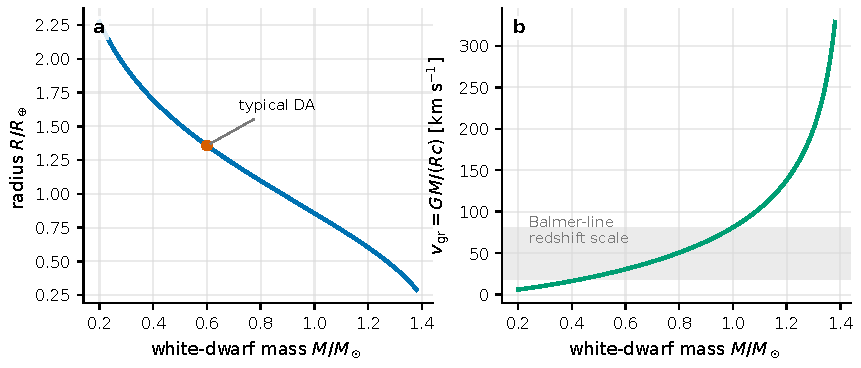
\includegraphics[width=0.94\linewidth]{figures/generated/chapter_11/ch11_white_dwarf_mass_radius.pdf}
\caption{As a white dwarf's mass increases its radius shrinks, contracting faster near the Chandrasekhar limit. The right panel converts the same mass--radius relation into the spectroscopically measurable gravitational-redshift velocity \(v_{\rm gr}=GM/(Rc)\); the Balmer-line redshift of a typical DA white dwarf is a few tens of \(\mathrm{km\,s^{-1}}\), already approaching or exceeding the velocity scale of ordinary stellar atmospheric motion.}
\label{fig:e18-wd-mr}
\end{figure}


\section{Small Angular Scale: Why Compact Objects Are So Hard to ``See Clearly''}
\label{sec:e18-angsize}

The previous section worked out that a white dwarf is only about the size of the Earth. This section translates this ``small'' into the quantity observers dread most: the angular diameter. Recall the definition from the imaging discussion of Chapter~\ref{chap:e11}: a disk of true diameter \(2R\) at distance \(d\) subtends an angle

\begin{equation}
  \theta_{\rm WD}=\frac{2R}{d}
  \simeq 11\,\mu\mathrm{as}
  \left(\frac{R}{0.012\,R_\odot}\right)
  \left(\frac{10\,\mathrm{pc}}{d}\right).
  \label{eq:e18-theta}
\end{equation}
\begin{formulaexplain}
\(\theta_{\rm WD}\): the white-dwarf angular diameter (microarcseconds \(\mu\mathrm{as}\)); \(R\): the radius; \(d\): the distance. Even as close as \(10\,\mathrm{pc}\), it is only about \(11\,\mu\mathrm{as}\), far beyond the resolving power of a single-aperture telescope.
\end{formulaexplain}

Lay out the numbers to feel it. \(1\,\mathrm{rad}=2.06\times10^{11}\,\mu\mathrm{as}\); \(10\,\mathrm{pc}=3.1\times10^{19}\,\mathrm{cm}\), \(R=0.012\,R_\odot=8.3\times10^8\,\mathrm{cm}\). Hence \(\theta=2R/d\approx5.3\times10^{-11}\,\mathrm{rad}\approx11\,\mu\mathrm{as}\). By comparison with Chapter~\ref{chap:e12}: an 8-meter telescope in the visible has a Rayleigh angle of about \(16\,\mathrm{mas}=1.6\times10^4\,\mu\mathrm{as}\) (converting with \(1\,\mathrm{mas}=10^3\,\mu\mathrm{as}\)), about three orders of magnitude larger than this white dwarf (\(1.6\times10^4/11\approx1.5\times10^3\)). Even with a 30-meter giant, the Rayleigh angle shrinks only to about \(4.3\,\mathrm{mas}\approx4.3\times10^3\,\mu\mathrm{as}\), still two to three orders of magnitude off. The conclusion is hard: \textbf{the spatial structure of compact objects is essentially hopeless for single-aperture imaging}.

So what to do? There are two ways out, both stages set up in the first half of this book. The first is to lengthen the baseline: the intensity interferometry of Chapter~\ref{chap:e10} measures the second-order coherence \(g^{(2)}\) between two telescopes separated by \(B\), with an equivalent resolving power of \(\lambda/B\). To resolve \(11\,\mu\mathrm{as}\), one needs a baseline of order \(B\sim\lambda/\theta\sim5\times10^{-5}\,\mathrm{cm}/5\times10^{-11}\approx10^6\,\mathrm{cm}=10\,\mathrm{km}\), exactly the scale the engineering plans of Chapters~\ref{chap:e22} and~\ref{chap:e24} aim to reach. The second way out is easier: since we cannot resolve the ``surface,'' let us not collide head-on with the spatial and instead go dig into the information in \emph{time} and \emph{polarization}. Compact objects spin fast and have strong fields, encoding much of the structural information in the light-curve phase and the polarization, exactly the main battlefield of the later sections of this chapter.

Here is a beautiful example of ``measuring physics without resolving'': gravitational redshift. A photon climbing out of a strong gravitational potential well loses energy and lengthens in wavelength, equivalent to a radial velocity

\begin{equation}
  v_{\rm gr}=\frac{GM}{Rc}
  \simeq 31.8\,\mathrm{km\,s^{-1}}
  \left(\frac{M}{0.6\,M_\odot}\right)
  \left(\frac{0.012\,R_\odot}{R}\right).
  \label{eq:e18-vgr}
\end{equation}
\begin{formulaexplain}
\(v_{\rm gr}\): the gravitational-redshift equivalent velocity, proportional to \(M/R\) (i.e., the compactness). The line redshift thus turns the mass--radius relation into a measurable velocity, no resolving of the stellar surface required.
\end{formulaexplain}

The derivation is one step: general relativity gives the fractional redshift \(\Delta\lambda/\lambda\simeq GM/(Rc^2)\) (weak-field limit), and multiplying by \(c\) gives the equivalent velocity \(v_{\rm gr}=GM/(Rc)\). It translates the ``heavier means smaller'' (\(\eqref{eq:e18-nauenberg}\)) white dwarf into a shift of a few tens of \(\mathrm{km\,s^{-1}}\) on the spectral lines, already exceeding the motion velocity of an ordinary stellar atmosphere and hence measurable. Of course, a real measurement must subtract the systemic peculiar velocity, the convective line shift, and the Stark shift, so large-sample work often averages the Gaia radii, the SDSS spectral line centers, and a kinematic model together. The right panel of Figure~\ref{fig:e18-wd-mr} is precisely this ``radius to velocity'' mapping.


\section{Magnetic White Dwarfs: How Accretion Geometry Is Written into Phase and Polarization}
\label{sec:e18-mcv}

There is a class of white dwarfs that carry a strong magnetic field: isolated magnetic white dwarfs have surface fields from \(10^6\) to \(10^9\,\mathrm{G}\), and the polars and intermediate polars in accreting binaries (cataclysmic variables) commonly have \(1\)--\(200\,\mathrm{MG}\). Here the magnetic field is no longer a supporting actor; it directly twines the structure problem together with the photon-statistics problem. First give the field an ``action radius.'' The magnetic moment of a magnetic dipole is the field strength times the radius cubed:

\begin{equation}
  \mu = B_* R_{\rm WD}^3
  \simeq 5.1\times10^{33}\,\mathrm{G\,cm^3}
  \left(\frac{B_*}{10\,\mathrm{MG}}\right)
  \left(\frac{R_{\rm WD}}{8\times10^8\,\mathrm{cm}}\right)^3 .
  \label{eq:e18-mu}
\end{equation}
\begin{formulaexplain}
\(\mu\): the magnetic moment (\(\mathrm{G\,cm^3}\)); \(B_*\): the surface field; \(R_{\rm WD}\): the radius. The larger the magnetic moment, the farther from the star the field can take over the accretion flow.
\end{formulaexplain}

Why compute the magnetic moment? Because the gas falling toward the white dwarf is ionized, and charged particles can only move along field lines. When the energy density of the field is enough to dominate the kinetic energy of the flow, the gas is ``taken over'' and forced to turn along the field lines toward the magnetic poles. The radius at which this takeover happens is called the magnetospheric radius:

\begin{equation}
  r_m \simeq k
  \left(\frac{\mu^4}{2GM\dot M^2}\right)^{1/7},
  \label{eq:e18-rm}
\end{equation}
\begin{formulaexplain}
\(r_m\): the magnetospheric radius; \(k\sim0.5\)--\(1\) is a geometric factor; \(\dot M\): the accretion rate. A larger magnetic moment pushes the magnetosphere farther out, and a higher accretion rate presses it closer in.
\end{formulaexplain}

That \(1/7\) power looks odd but in fact comes from the balance ``magnetic pressure equals the ram pressure of the infall'': magnetic pressure \(\propto B^2\propto\mu^2/r^6\), infall ram pressure \(\propto\dot M\sqrt{GM/r}/r^2\propto r^{-5/2}\), and setting the two equal and solving gives \(r_m\propto(\mu^4/GM\dot M^2)^{1/7}\): the exponents \(4\), \(1\), \(2\), and \(7\) are all balanced out this way. The \(\dot M\) of cataclysmic variables ranges from \(10^{-11}\) to \(10^{-8}\,M_\odot\,\mathrm{yr^{-1}}\), and the magnetosphere size floats accordingly from near the stellar surface to tens of stellar radii.

The magnetosphere size becomes meaningful only when compared with another radius: the corotation radius, the place where the angular velocity at which the field rigidly corotates with the star exactly equals the Keplerian orbital angular velocity:

\begin{equation}
  r_{\rm co}=\left(\frac{GM}{\Omega_s^2}\right)^{1/3},
  \label{eq:e18-rco}
\end{equation}
\begin{formulaexplain}
\(r_{\rm co}\): the corotation radius; \(\Omega_s\): the white dwarf's rotation angular velocity. Here the speed at which ``the field drags things around'' equals the ``orbiting speed gravity allows,'' the watershed for whether accretion can smoothly fall.
\end{formulaexplain}

Its derivation is also one step: set the centrifugal force \(\Omega_s^2 r\) corresponding to the corotation linear velocity equal to gravity \(GM/r^2\), and solve for \(r_{\rm co}=(GM/\Omega_s^2)^{1/3}\). The physical criterion is very intuitive: if \(r_m<r_{\rm co}\), matter is taken over by the field within the corotation radius and can fall fairly smoothly along the field lines to the magnetic poles; if \(r_m\gtrsim r_{\rm co}\), the field lines are already spinning faster than Keplerian at the takeover point and will \emph{fling} matter away, forming a ``propeller''-type ejection or altering the flow morphology. Observationally, the \(P_{\rm spin}/P_{\rm orb}\) of intermediate polars is often \(0.01\)--\(0.6\), while polars are nearly synchronous (\(P_{\rm spin}\simeq P_{\rm orb}\)) \citep{1970ApJ...160L.147A,2000PASP..112..873W,1991MNRAS.249..460W,2008ApJ...672..524N}. Figure~\ref{fig:e18-mcv-map} plots out this classification of ``geometry determined by magnetic moment and rotation speed.''

\begin{figure}[tbp]
\centering
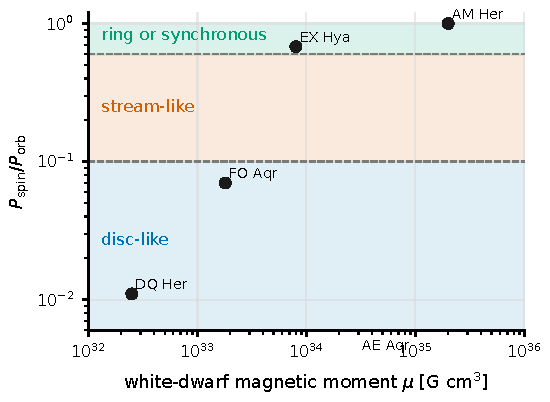
\includegraphics[width=0.78\linewidth]{figures/generated/chapter_11/ch11_magnetic_cv_flow_map.pdf}
\caption{The accretion flow of a magnetic cataclysmic variable is determined mainly by the white dwarf's magnetic moment and the speed of its rotation relative to the orbit. Low-\(P_{\rm spin}/P_{\rm orb}\) systems tend to form disk-like flows, the intermediate region often shows magnetically controlled flows, and near-synchronous or high-ratio systems shift toward ring, stream, or polar-system geometries; these geometries directly change the light-curve phase, circular polarization, and correlation functions.}
\label{fig:e18-mcv-map}
\end{figure}

The falling flow releases gravitational potential energy, turning it into light. The order of magnitude is given by the depth of the potential well times the mass flow rate:

\begin{equation}
  L_{\rm acc}\simeq \frac{GM\dot M}{R_{\rm WD}}
  \simeq 1.0\times10^{33}\,\mathrm{erg\,s^{-1}}
  \left(\frac{M}{0.8\,M_\odot}\right)
  \left(\frac{\dot M}{10^{-10}M_\odot\,\mathrm{yr^{-1}}}\right)
  \left(\frac{8\times10^8\,\mathrm{cm}}{R_{\rm WD}}\right).
  \label{eq:e18-lacc}
\end{equation}
\begin{formulaexplain}
\(L_{\rm acc}\): the accretion luminosity (\(\mathrm{erg\,s^{-1}}\)), equal to the gravitational potential energy released per unit time \(GM\dot M/R\). It gives the order of magnitude of the photon rate available in such systems; the optical receives only a portion of it.
\end{formulaexplain}

This luminosity is a blend of various components: the accretion disk, hot spots near the magnetic poles, the columnar shock region, the illuminated white-dwarf surface, and \emph{cyclotron emission}. Here we connect to a pedagogical focus of this chapter: how a strong field writes polarization into the light. A charged electron in a magnetic field spirals around the field lines, and the angular frequency of that spiraling is the cyclotron frequency
\[
  \omega_c=\frac{eB}{m_e c},
  \qquad
  \hbar\omega_c\approx 11.6\,\mathrm{keV}\left(\frac{B}{10^{12}\,\mathrm{G}}\right).
\]
An electron going in circles is an accelerating charge and radiates; the radiation is concentrated at \(\omega_c\) and its harmonics. For magnetic white dwarfs with \(B\sim10\)--\(200\,\mathrm{MG}=10^7\)--\(2\times10^8\,\mathrm{G}\), the fundamental photon energy \(\hbar\omega_c\sim0.1\)--\(2\,\mathrm{eV}\), plus several harmonics, falls right in the near-infrared to optical: this is why the optical light curve of a polar shows a string of ``cyclotron humps.'' The key point: an electron circling the field lines radiates with natural \emph{polarization}: looking along the field lines you see circular polarization, looking sideways you see linear polarization. So polarization becomes the probe that \emph{picks out} the cyclotron component from the disk light and the blackbody light. (Replace the non-relativistic cyclotron radiation with relativistic electrons, and it is the synchrotron radiation discussed in Chapter~\ref{chap:e16}; the two are the two faces of the same mechanism in different energy bands.)

How does polarization read the geometry? Two empirical rules are very useful. First, if the \emph{sign} of the circular polarization flips with rotation phase, it usually means the line of sight has swept across different magnetic poles, or the projected field direction has changed sign. Second, if the linear-polarization peak and the total light-curve peak are \emph{not synchronous}, it says the ``brightest region'' and the ``region of most special field geometry'' are not the same patch: the intensity peak comes from shock-region heating, while the polarization peak comes from field projection.

How should these phase modulations be quantified in the event table? Bin the photons by white-dwarf rotation phase \(\phi_s\), and within each phase window compute the second-order intensity correlation (the \(g^{(2)}\) of Chapter~\ref{chap:e08}):

\begin{equation}
  g^{(2)}_{\phi_s}(\tau)=
  \frac{\langle I_{\phi_s}(t)\,I_{\phi_s}(t+\tau)\rangle}
       {\langle I_{\phi_s}(t)\rangle^2}.
  \label{eq:e18-g2phi}
\end{equation}
\begin{formulaexplain}
\(g^{(2)}_{\phi_s}(\tau)\): the second-order intensity correlation within a fixed rotation-phase window \(\phi_s\); \(I_{\phi_s}\): the count rate within that window. It extracts the ``short-term memory'' at delay \(\tau\) of the same magnetic pole or the same segment of accretion flow.
\end{formulaexplain}

The reading must be careful about timescales. If \(\tau\) is milliseconds to seconds, the structure of \(g^{(2)}\) may come from shock-region cooling, magnetically controlled clumps, or purely spurious signal from detector dead time; if \(\tau\) is tens of seconds to minutes, it is more like classical flickering or atmospheric transparency fluctuations than the compact source itself. And an iron rule: the average in \(\eqref{eq:e18-g2phi}\) \emph{must} be taken within the same phase window, the same energy band, and the same polarization channel, or else the orbital modulation will be mistaken for short-term correlation: this is exactly the weight the phrase ``phase-resolved'' carries.


\section{Neutron Stars: How the Magnetosphere Is Sliced into a Phase Event Table}
\label{sec:e18-nsphase}

A neutron star is an order of magnitude smaller still than a white dwarf: the radius is only \(10\)--\(14\,\mathrm{km}\), while the mass is often \(1.2\)--\(2.2\,M_\odot\). Such a small object spins extremely fast and has an extremely strong field, so its magnetosphere is ``sliced'' by rotation into a set of natural phase coordinates. The most basic boundary line is the light-cylinder radius: the place where the linear velocity of rigid corotation exactly reaches the speed of light:

\begin{equation}
  R_{\rm LC}=\frac{c}{\Omega}=\frac{cP}{2\pi}
  \simeq 1.6\times10^3\,\mathrm{km}
  \left(\frac{P}{33\,\mathrm{ms}}\right).
  \label{eq:e18-rlc}
\end{equation}
\begin{formulaexplain}
\(R_{\rm LC}\): the light-cylinder radius; \(P\): the rotation period; \(\Omega=2\pi/P\): the angular velocity. Here ``rigidly corotating with the star'' would require reaching the speed of light, so it is the outermost boundary that open field lines, particle acceleration, and high-energy radiation can be organized within.
\end{formulaexplain}

The derivation is one sentence: set the corotation linear velocity \(v=\Omega r\) equal to \(c\), and solve for \(r=c/\Omega=cP/2\pi\). The order of magnitude is quite vivid: the Crab pulsar has \(P\simeq33\,\mathrm{ms}\), light cylinder about \(1600\,\mathrm{km}\); millisecond pulsars have \(P\simeq1.5\)--\(10\,\mathrm{ms}\), light cylinder only tens to hundreds of km; a magnetar has \(P\simeq2\)--\(12\,\mathrm{s}\), light cylinder up to \(10^5\,\mathrm{km}\) and beyond. Within \(R_{\rm LC}\) the field lines are closed and corotate with the star; beyond it they must open, and particles accelerate and radiate along the open field lines. The discovery of pulsars and the interpretation as ``rotating neutron stars'' established this picture, and the Crab further linked rotational energy loss to a supernova remnant \citep{1968Natur.217..709H,1968Natur.218..731G,1968Natur.219..145P,1972ApJ...175..217B}. Figure~\ref{fig:e18-lc} draws the linear growth of the light cylinder with period and the Crab-type phase profile.

\begin{figure}[tbp]
\centering
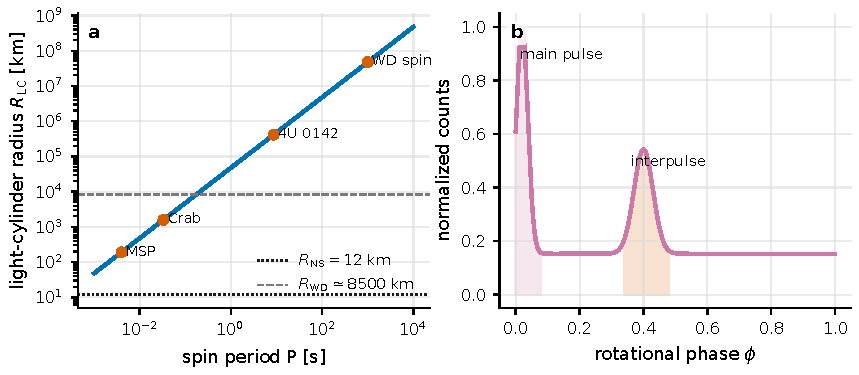
\includegraphics[width=0.94\linewidth]{figures/generated/chapter_11/ch11_light_cylinder_phase.pdf}
\caption{The light-cylinder radius increases linearly with rotation period. A millisecond pulsar's light cylinder is only tens to hundreds of km, the Crab's about \(1.6\times10^3\,\mathrm{km}\), and a magnetar's can reach \(10^5\,\mathrm{km}\) and beyond. The right panel is a Crab-type phase-folded profile, where the phase windows of the main pulse and interpulse determine which photons enter the subsequent intensity correlation or polarization statistics.}
\label{fig:e18-lc}
\end{figure}

How strong is the field? We cannot measure the neutron-star surface, but we can infer it from its ever-slowing rotation. A magnetized rotating body is like an antenna, radiating a magnetic-dipole wave outward and carrying away energy, so the rotation slows. The intermediate bridge for this step is the magnetic-dipole radiation formula: a dipole of magnetic moment \(m=B R^3\), rotating at angular velocity \(\Omega\), with the magnetic axis at angle \(\chi\) to the rotation axis, radiates the power (the classical Larmor formula generalized to a rotating magnetic dipole)
\[
  \dot E_{\rm dip}=\frac{B^2R^6\Omega^4\sin^2\chi}{6c^3}.
\]
Setting this radiative loss equal to the loss of rotational kinetic energy \(\dot E=I\Omega\dot\Omega\) (the next equation~\eqref{eq:e18-edot} will expand it), equating the two, solving for \(B\), then substituting the standard assumptions \(R=10\,\mathrm{km}\), \(I=10^{45}\,\mathrm{g\,cm^2}\), \(\sin\chi=1\), and converting \(\Omega=2\pi/P\), \(\dot\Omega=-2\pi\dot P/P^2\) into period, one tidies up the equatorial surface field

\begin{equation}
  B_{\rm dip}\simeq 3.2\times10^{19}\,(P\dot P)^{1/2}\,\mathrm{G}.
  \label{eq:e18-bdip}
\end{equation}
\begin{formulaexplain}
\(B_{\rm dip}\): the dipole field inferred from rotational slowdown (\(\mathrm{G}\)); \(P\) in seconds, \(\dot P\) (dimensionless \(\mathrm{s\,s^{-1}}\)) the rate of change of the period. It translates the ``spinning down'' in the timing data into a field scale.
\end{formulaexplain}

The numbers tell us how outrageous the neutron-star field is: ordinary young pulsars have \(B_{\rm dip}\sim10^{11}\)--\(10^{13}\,\mathrm{G}\), and magnetars can reach \(10^{14}\)--\(10^{15}\,\mathrm{G}\); the Earth's field is only \(0.5\,\mathrm{G}\), and even the strongest laboratory steady-state field is only of order \(10^5\,\mathrm{G}\). This field is the stage behind vacuum birefringence. The rate of energy released by slowdown is

\begin{equation}
  \dot E = 4\pi^2 I\,\frac{\dot P}{P^3},
  \qquad
  I\simeq10^{45}\,\mathrm{g\,cm^2}.
  \label{eq:e18-edot}
\end{equation}
\begin{formulaexplain}
\(\dot E\): the rotational-energy loss rate (\(\mathrm{erg\,s^{-1}}\)); \(I\): the moment of inertia (about \(10^{45}\,\mathrm{g\,cm^2}\)). It is the total energy budget for the pulsar to drive magnetospheric radiation and the nebula.
\end{formulaexplain}

Derivation: the rotational kinetic energy \(E=\tfrac12 I\Omega^2=2\pi^2 I/P^2\), differentiated in time gives \(\dot E=-4\pi^2 I\dot P/P^3\) (the positive sign denoting the loss rate). The Crab's \(\dot E\sim10^{38}\,\mathrm{erg\,s^{-1}}\) is enough to light up the pulses from radio to \(\gamma\)-rays and the entire Crab nebula \citep{1984ApJ...283..279H,1992ApJ...397..187B,2001A&A...378..918K,2008ApJ...680.1378H}.

Now send the photons into the phase coordinate. Each photon first receives a barycentric correction (subtracting the arrival-time difference caused by the Earth's orbital motion), then is folded into a phase using the timing ephemeris:

\begin{equation}
  \phi_i=
  \left[
  \nu(t_i-t_0)+\tfrac12\dot\nu(t_i-t_0)^2
  +\tfrac16\ddot\nu(t_i-t_0)^3+\cdots
  \right]\bmod 1 .
  \label{eq:e18-fold}
\end{equation}
\begin{formulaexplain}
\(\phi_i\): the rotation phase of the \(i\)-th photon (\(0\)--\(1\)); \(t_i\): its barycentric arrival time; \(\nu=1/P\) and \(\dot\nu,\ddot\nu\): the rotation frequency and its derivatives. Taking \(\bmod\,1\) rolls the long arrival-time table into a single cycle of phase.
\end{formulaexplain}

Term by term: \(t_i\) is the barycentric time (seconds), \(t_0\) is the reference epoch, \(\nu\) describes the basic rotation, \(\dot\nu\) describes the slowdown, and \(\ddot\nu\) describes higher-order terms such as post-glitch recovery. This step rolls ``a long string of arrival times'' into ``one cycle of phase from \(0\) to \(1\),'' and superposing many cycles gives a high-signal-to-noise pulse profile (Figure~\ref{fig:e18-lc}, right). The Crab's main-pulse width occupies only about \(0.04\)--\(0.05\) in phase, and radio giant pulses can be as narrow as microseconds. Interestingly: picking out the rotation cycles in which giant radio pulses occur, the optical main pulse is on average enhanced by about \(3\%\), while the pulse shape and arrival phase are essentially unchanged; the energy-resolved photon counting of ARCONS further shows that the optical enhancement corresponding to early-arriving giant radio pulses can reach a dozen to a couple dozen percent \citep{2003Sci...301..493S,2013ApJ...779L..12S}. These results connect the coherent radio bursts and the incoherent optical radiation to the same portion of magnetospheric plasma, a connection visible only when the radio and the optical are placed in the \emph{same phase event table}.

With the phase coordinate in hand, one can do phase-resolved second-order correlation, comparing the synchronous fluctuations of different energy bands, polarizations, or telescopes at the same pulse phase:

\begin{equation}
  g^{(2)}_{ab}(\tau\mid\Phi)=
  \frac{\langle n_a(t,\Phi)\,n_b(t+\tau,\Phi)\rangle}
       {\langle n_a(t,\Phi)\rangle\langle n_b(t,\Phi)\rangle},
  \label{eq:e18-g2ab}
\end{equation}
\begin{formulaexplain}
\(g^{(2)}_{ab}(\tau\mid\Phi)\): the cross-correlation of channels \(a\) and \(b\) within the phase window \(\Phi\); \(n_a,n_b\): the counts of the two channels. \(a,b\) can be energy bands, polarizations, or different telescopes, used to examine synchronicity at the same pulse phase.
\end{formulaexplain}

For a bright source like the Crab, \(\tau\) can be pushed to microseconds to milliseconds, truly approaching single-pulse statistics; for fainter optical pulsars, the first thing achievable is usually still only the luminosity and polarization stacking within a phase window, still far from pulse-by-pulse correlation \citep{1996ApJ...468..779M,2000ApJ...537..861S,2009MNRAS.397..103S}. When \(a,b\) here point to different telescopes, \(\eqref{eq:e18-g2ab}\) connects directly to the intensity interferometry of Chapter~\ref{chap:e10}, only now each \(g^{(2)}\) hangs on a rotation-phase label.


\section{Strong-Field Polarization: The Imprint of Vacuum Birefringence and QED Strong-Field Effects}
\label{sec:e18-qed}

This section walks to the most ``quantum'' place in the chapter's physics. In classical electrodynamics the vacuum is empty, bends no light, and separates no polarization. But quantum electrodynamics (QED) says: the vacuum in fact seethes with virtual electron--positron pairs, and a strong field \emph{polarizes} them, turning the vacuum into a medium with a preferred polarization direction, birefringent like a calcite crystal. This effect is called vacuum birefringence. When does it grow strong? The yardstick is the QED critical field:

\begin{equation}
  B_Q=\frac{m_e^2c^3}{e\hbar}=4.414\times10^{13}\,\mathrm{G}.
  \label{eq:e18-bq}
\end{equation}
\begin{formulaexplain}
\(B_Q\): the QED critical field. At this field strength, the cyclotron energy of the lowest Landau level of the electron already approaches its rest energy \(m_ec^2\), and the quantum magnetic effect is no longer a small correction. A magnetar surface \(B\) approaches or even exceeds \(B_Q\).
\end{formulaexplain}

The physical meaning of \(B_Q\) is worth savoring: set \(\hbar\omega_c=\hbar eB/(m_ec)\) equal to the electron rest energy \(m_ec^2\), and the solution is precisely \(B=m_e^2c^3/(e\hbar)=B_Q\). That is to say, when the field is so strong that ``the quantum energy of one electron cyclotron loop equals its entire rest mass,'' the quantum structure of the vacuum can no longer be ignored. A magnetar surface \(B\sim10^{14}\)--\(10^{15}\,\mathrm{G}\) is an order of magnitude larger than \(B_Q\): vacuum birefringence here is no armchair theorizing.

When \(B\ll B_Q\) and the photon energy is far below \(m_ec^2\), the Heisenberg--Euler effective theory gives the refractive-index difference between the two polarization normal modes (weak-field approximation):

\begin{equation}
  \Delta n\simeq\frac{\alpha_{\rm fs}}{30\pi}
  \left(\frac{B_\perp}{B_Q}\right)^2 ,
  \label{eq:e18-dn}
\end{equation}
\begin{formulaexplain}
\(\Delta n\): the refractive-index difference between the parallel and perpendicular polarization normal modes; \(B_\perp\): the field component perpendicular to the light ray; \(\alpha_{\rm fs}\simeq1/137\): the fine-structure constant. It grows as \(B_\perp^2\): double the field, and the birefringence quadruples.
\end{formulaexplain}

Note \(\Delta n\propto B_\perp^2\): the field is the ``accelerator'' of this effect, and it is stepped on hard. The magnetar surface field exceeds \(B_Q\), so the weak-field formula can no longer serve as an exact model, but it lays bare the crux: \emph{polarization is extremely sensitive to the strong field}. The two polarization modes propagate in the vacuum at slightly different speeds, accumulating a phase difference along the light path:

\begin{equation}
  \Delta\Phi(E)=\frac{E}{\hbar c}\int\Delta n(s)\,ds .
  \label{eq:e18-dphi}
\end{equation}
\begin{formulaexplain}
\(\Delta\Phi(E)\): the phase difference accumulated by the two polarization modes; \(E\): the photon energy; the integral runs along the light path \(s\). The higher the energy and the larger the \(\Delta n\) along the path, the stronger the polarization-propagation effect.
\end{formulaexplain}

This phase difference brings an observable consequence, called polarization freezing. Imagine photons setting out from different small patches on the magnetar surface, each patch with a different field direction and hence a different polarization direction. Without vacuum birefringence, these randomly oriented polarizations superposed would cancel each other, and the observed net polarization degree would be low. But with birefringence, as long as the propagation is adiabatic, the polarization vector \emph{locks} onto the local field direction and rotates slowly with the field, freezing out only at the far ``polarization-limiting radius.'' The result: the polarization directions from a large area of the stellar surface are ``combed'' into alignment by the field, cancellation is reduced, and the net polarization degree instead \emph{rises}. So \textbf{a high polarization degree is itself an indirect imprint of vacuum birefringence}. This picture comes from the combination of strong-field QED, magnetospheric propagation, and neutron-star surface radiation models \citep{1936ZPhy...98..714H,1971AnPhy..67..599A,2000MNRAS.311..555H,2002PhRvD..66b3002H,2003MNRAS.342..134H}. An X-ray polarimeter (such as IXPE) works at \(2\)--\(8\,\mathrm{keV}\), precisely to measure this polarization in this energy band.

So how exactly are ``polarization degree'' and ``polarization angle'' computed from the photons? This is the core tool shared by this chapter and Chapter~\ref{chap:e22}. An X-ray polarimeter measures an azimuthal angle (modulation angle) \(\eta_i\) for each photoelectric event, then accumulates many events into the Stokes parameters (the total intensity \(I\) below is the same symbol as, but a different quantity from, the moment of inertia \(I\) of~\eqref{eq:e18-edot}; do not confuse them):

\begin{equation}
  I=\sum_i w_i,\qquad
  Q=\sum_i w_i\cos 2\eta_i,\qquad
  U=\sum_i w_i\sin 2\eta_i .
  \label{eq:e18-stokes}
\end{equation}
\begin{formulaexplain}
\(I\): the total intensity; \(Q,U\): the two linear-polarization Stokes components; \(\eta_i\): the azimuthal angle of the \(i\)-th event; \(w_i\): the weight (including instrument modulation, background, and effective-area factors). The factor \(2\) in front of the angle reflects that polarization is ``undirected'': rotating \(180^\circ\) returns to itself.
\end{formulaexplain}

Why \(\cos2\eta\) rather than \(\cos\eta\)? Because polarization is an \emph{undirected line}: rotating the polarization direction by \(180^\circ\) is the same as not rotating it, so the physical quantity must have period \(2\eta\). Weighting and summing the azimuthal angles of a large number of events this way, the random directions cancel each other, and only the truly polarized direction leaves a net vector in \(Q,U\). From it we obtain the polarization degree and polarization angle:

\begin{equation}
  p=\frac{\sqrt{Q^2+U^2}}{I},\qquad
  \psi=\tfrac12\arctan2(U,Q).
  \label{eq:e18-pdop}
\end{equation}
\begin{formulaexplain}
\(p\): the linear polarization degree (\(0\)--\(1\)); \(\psi\): the polarization angle. The \emph{length} of the two-dimensional vector \((Q,U)\) gives the polarization strength, and its \emph{direction} (after dividing by 2) gives the polarization angle on the sky.
\end{formulaexplain}

Plug in a real number: optical polarization measurements of the isolated neutron star RX J1856.5\(-\)3754 gave \(p=16.43\%\pm5.26\%\), while the source itself is as faint as \(V\simeq25.5\); the foreground interstellar polarization and the instrument polarization must both be subtracted item by item. Such an elevated polarization degree, compared against thermal surface models, supports vacuum birefringence having reduced the polarization cancellation of different surface regions \citep{2015MNRAS.454.3254T,2016MNRAS.459.3585G,2017MNRAS.465..492M}. Figure~\ref{fig:e18-stokes} shows how the rotating magnetic geometry projects the polarization into phase curves of \(Q/I\), \(U/I\) and a track on the Q--U plane.

\begin{figure}[tbp]
\centering
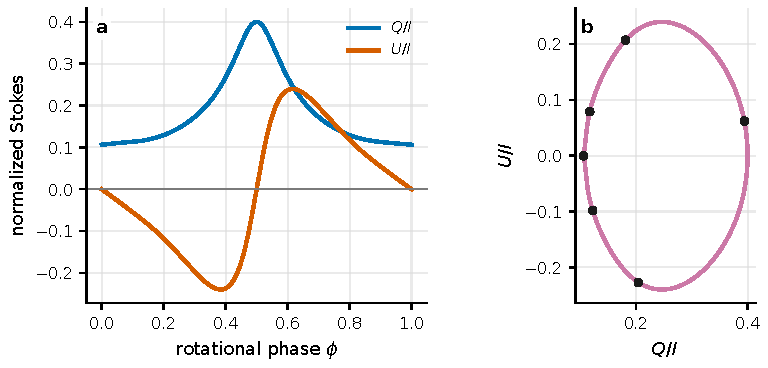
\includegraphics[width=0.92\linewidth]{figures/generated/chapter_11/ch11_stokes_qu_track.pdf}
\caption{The rotating magnetic geometry projects the polarization-angle variation into phase curves of \(Q/I\) and \(U/I\). The left panel shows the two Stokes components given by the same phase event table, and the right panel shows the corresponding Q--U track; the shape of the track exposes geometric degeneracy and instrument crosstalk better than the polarization degree alone.}
\label{fig:e18-stokes}
\end{figure}

How does the polarization angle swing with phase? To first approximation one uses the rotating vector model:

\begin{equation}
  \tan(\psi-\psi_0)=
  \frac{\sin\alpha\,\sin(\phi-\phi_0)}
       {\sin\zeta\cos\alpha-\cos\zeta\sin\alpha\cos(\phi-\phi_0)} .
  \label{eq:e18-rvm}
\end{equation}
\begin{formulaexplain}
\(\psi\): the polarization angle; \(\alpha\): the angle between the magnetic axis and the rotation axis; \(\zeta\): the angle between the line of sight and the rotation axis; \(\phi\): the rotation phase; \(\psi_0,\phi_0\): the zero points. It translates ``the S-shaped swing of the polarization angle with phase'' into the geometric orientation of the magnetosphere.
\end{formulaexplain}

This equation was first used for the polarization geometry of radio pulsars: it is purely the spherical trigonometry of ``projecting the field lines onto the sky.'' But in magnetar X-rays, it is only a low-dimensional geometric skeleton, because surface radiation, resonant cyclotron scattering, and vacuum birefringence together rewrite \(p(E,\phi)\) and \(\psi(E,\phi)\), making the measured polarization far richer than pure geometry \citep{1969ApL.....3..225R,2018ApJ...854...98W,2011ApJ...730..131F}.

Consider a real example that twines these clues together: the magnetar 4U 0142+61 (Figure~\ref{fig:e18-biref}). IXPE in the full \(2\)--\(8\,\mathrm{keV}\) band saw a linear polarization degree of \(12\%\pm1\%\), but split by energy band the story is more remarkable: low energy \(2\)--\(4\,\mathrm{keV}\) polarization degree \(14\%\pm1\%\), high energy \(5.5\)--\(8\,\mathrm{keV}\) soaring to \(41\%\pm7\%\), while in the intermediate range near \(4\)--\(5\,\mathrm{keV}\) the polarization degree drops to the sensitivity floor and the polarization angle even flips by about \(90^\circ\). This \(90^\circ\) flip is the key fingerprint: it means the two polarization normal modes (the O mode and the X mode) ``switch shifts'' at this energy: at low energy one mode dominates, at high energy the other, and at the crossover the two cancel and the direction turns around. The source's rotation period is \(P=8.69\,\mathrm{s}\), the field \(B\sim10^{14}\,\mathrm{G}\), the soft X-ray has a blackbody component with \(kT\sim0.5\)--\(1\,\mathrm{keV}\), and the hard tail extends to tens or even hundreds of keV. In explaining this dataset, the low-energy O mode, the hard-tail X mode, a surface condensate or thin atmosphere, and resonant Compton scattering may all participate; a \emph{single} high-polarization point alone is not yet enough to determine vacuum birefringence on its own, and requires cross-validation across energy, phase, and multiple sources \citep{2022Sci...378..646T,2023A&A...674L..10C,2023MNRAS.519.3681F}.

\begin{figure}[tbp]
\centering
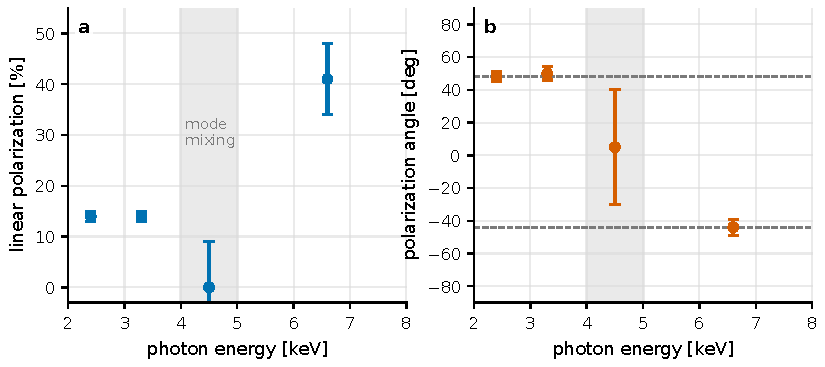
\includegraphics[width=0.92\linewidth]{figures/generated/chapter_11/ch11_birefringence_energy.pdf}
\caption{The IXPE result on the magnetar 4U 0142+61 can be viewed as a switching of the two polarization normal modes with energy. Low energy \(2-4\,\mathrm{keV}\) polarization degree about \(14\%\), high energy \(5.5-8\,\mathrm{keV}\) rising to about \(41\%\), while near \(4-5\,\mathrm{keV}\) the polarization degree approaches the minimum detectable polarization and the polarization angle flips by about \(90^\circ\).}
\label{fig:e18-biref}
\end{figure}

Bring this section back to the main thread of the book. Each step above (measuring \(\eta_i\), accumulating the Stokes parameters, computing \(p\) and \(\psi\), binning by phase and energy) is in essence \textbf{doing intensity/count statistics on the polarization channel}. It is the same family of tools as the \(g^{(2)}\) of Chapter~\ref{chap:e08} and the intensity interferometry of Chapter~\ref{chap:e10}: only now the ``two telescopes'' or ``two instants'' are replaced by ``two polarization bases.'' Chapter~\ref{chap:e22} will formally develop this ``polarization quantum channel,'' discussing its use in the search for new physics such as dark matter and axions; the magnetar birefringence here is the cleanest training ground for this channel on strong-field objects.


\section{Surface and Atmospheric Radiation: How Hot-Spot Light Curves Infer the Neutron-Star Radius}
\label{sec:e18-hotspot}

Finally, we return to the old problem of ``what to do when we cannot resolve,'' but switched to the neutron star, the answer is especially beautiful. The neutron-star radius cannot be measured through the angular diameter (Section~\ref{sec:e18-angsize} said it is even smaller than a white dwarf), yet it can be measured to \(\sim1\,\mathrm{km}\) precision: relying not on spatial resolution but on \emph{light-curve shape + energy spectrum + general relativity}. The core quantity is the compactness:

\begin{equation}
  u=\frac{2GM}{Rc^2}
  \simeq 0.345
  \left(\frac{M}{1.4\,M_\odot}\right)
  \left(\frac{12\,\mathrm{km}}{R}\right).
  \label{eq:e18-compact}
\end{equation}
\begin{formulaexplain}
\(u\): the compactness, equal to the ratio of the Schwarzschild radius \(2GM/c^2\) to the true radius \(R\) (dimensionless). The larger \(u\), the stronger the gravitational bending of light, and the more easily the amplitude of the hot-spot light curve is smoothed away.
\end{formulaexplain}

The physical picture: the neutron-star surface often has one or two spots hotter than their surroundings (hot spots near the magnetic poles). As the star rotates, the hot spot sweeps across the line of sight and we see pulsation. But the neutron star's gravity is strong enough to \emph{bend} light: a hot spot that has rotated to the far side and should be invisible has its emitted light dragged back into our line of sight by gravity. The larger the compactness, the harder the bending, and the more the far-side spot can ``leak'' through, so the pulse troughs are raised and the amplitude flattened. Writing this bending effect as a useful approximation, relating the emission angle \(\alpha\) at which the photon leaves the surface (here \(\alpha\) is the geometric emission angle, the same symbol as, but a different quantity from, the fine-structure constant \(\alpha_{\rm fs}\) earlier and the magnetic-axis angle \(\alpha\) in the rotating vector model) and the central angle \(\psi\) of the hot spot relative to the line of sight (here \(\psi\) is the spatial angular distance, not the polarization angle \(\psi\) of~\eqref{eq:e18-pdop} and~\eqref{eq:e18-rvm}):

\begin{equation}
  \cos\alpha\simeq u+(1-u)\cos\psi .
  \label{eq:e18-bending}
\end{equation}
\begin{formulaexplain}
\(\alpha\): the emission angle of the photon leaving the stellar surface relative to the normal; \(\psi\): the angular distance of the hot-spot center relative to the line of sight. This linear approximation writes ``whether a spot is still visible after bending'' as a simple function of the compactness \(u\).
\end{formulaexplain}

It applies to the Schwarzschild exterior spacetime and scaling estimates from slow to moderate rotation; a real millisecond pulsar must further add Doppler boosting, aberration, time delay, stellar oblateness, and atmospheric beaming. Figure~\ref{fig:e18-hotspot} shows that at low compactness the pulse amplitude is large, and at high compactness the trough is raised: radius inference exploits exactly this change in profile \citep{2002ApJ...566L..85B,2019AIPC.2127b0008W}.

\begin{figure}[tbp]
\centering
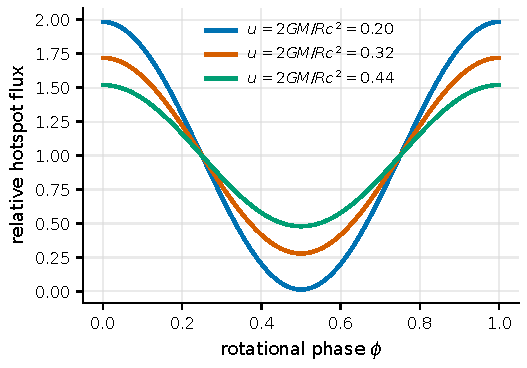
\includegraphics[width=0.78\linewidth]{figures/generated/chapter_11/ch11_hotspot_lightcurve.pdf}
\caption{The hot-spot light curve is very sensitive to compactness. At low compactness, the spot's contribution vanishes quickly after it rotates to the far side, and the pulse amplitude is large; at high compactness, gravitational light bending makes a larger area of the surface visible, and the light-curve trough is raised. Radius inference exploits this profile change and fits it jointly with mass, inclination, hot-spot position, and atmospheric beaming.}
\label{fig:e18-hotspot}
\end{figure}

How to turn this physics into a measurement of \(M,R\)? The key is to realize: all we have in hand is an \emph{event table}: each X-ray photon carries an energy and a rotation phase. Compute the astrophysical model (hot-spot geometry + atmosphere + gravitational bending) forward into ``how many photons there should be in each energy channel and each phase bin,'' then compare with the measurement. The expected count in the \(j\)-th energy channel and \(k\)-th phase bin is
\begin{equation}
  \lambda_{jk}(\Theta)=
  T\int dE\,R_j(E)\,
  \left[F_E(\phi_k;\Theta)+B_E\right].
  \label{eq:e18-lambda}
\end{equation}
\begin{formulaexplain}
\(\lambda_{jk}\): the expected count in energy channel \(j\), phase bin \(k\); \(T\): the exposure time; \(R_j(E)\): the instrument response (effective area + energy redistribution); \(F_E\): the hot-spot model flux; \(B_E\): the background. \(\Theta\) holds all the parameters: \(M,R\), distance, inclination, hot-spot position, etc. It translates the astrophysical model into the expected number of events in the detector.
\end{formulaexplain}

The parameter vector \(\Theta\) is packed with \(M,R\), distance, observer inclination, hot-spot latitude and longitude, hot-spot angular radius, temperature, and atmospheric parameters, a whole set. The measured count will of course not exactly equal \(\lambda_{jk}\); it follows Poisson statistics (Chapter~\ref{chap:e03}): given the expectation \(\lambda\), the probability of observing \(N\) is \(e^{-\lambda}\lambda^N/N!\). Multiplying the probabilities over all energy channels and phase bins and taking the logarithm gives the Poisson log-likelihood:
\begin{equation}
  \ln\mathcal{L}(\Theta)=
  \sum_{j,k}\left[
  N_{jk}\ln\lambda_{jk}(\Theta)-\lambda_{jk}(\Theta)-\ln(N_{jk}!)
  \right].
  \label{eq:e18-lnl}
\end{equation}
\begin{formulaexplain}
\(\ln\mathcal{L}\): the Poisson log-likelihood; \(N_{jk}\): the measured count. Multiplying \(e^{-\lambda}\lambda^N/N!\) over all \((j,k)\) and taking the logarithm gives it. Finding the radius means finding a set of \(\Theta\) that makes all \(\lambda_{jk}\) fit the event table best.
\end{formulaexplain}

The derivation needs only one step: \(\ln\prod_{jk}\dfrac{e^{-\lambda_{jk}}\lambda_{jk}^{N_{jk}}}{N_{jk}!}=\sum_{jk}\big(-\lambda_{jk}+N_{jk}\ln\lambda_{jk}-\ln N_{jk}!\big)\). The last term \(\ln N_{jk}!\) contains no parameters and is a constant in the fit, which may be dropped. What remains is the objective to be \emph{maximized}: this is exactly the general paradigm of event-table modeling of Chapter~\ref{chap:e13}, only that the ``astrophysical model'' here is packed with gravitational bending and a strong-field atmosphere. The NICER radius measurements of PSR J0030+0451 and PSR J0740+6620 were done just this way: the J0740 analysis combined the NICER event table, the XMM-Newton imaging-spectroscopy background, and the mass and distance priors from radio timing, and Riley et al. obtained \(R=12.39^{+1.30}_{-0.98}\,\mathrm{km}\), \(M=2.072^{+0.067}_{-0.066}\,M_\odot\), while Miller et al. gave a constraint from a different method but consistent; the two independent analyses of J0030 further show that the hot-spot geometry may carry a complex multipole field structure \citep{2019ApJ...887L..21R,2019ApJ...887L..24M,2021ApJ...918L..27R,2021ApJ...918L..28M}. Appreciate the weight of this: we did not resolve a \(12\,\mathrm{km}\) sphere (that would require nanoarcsecond resolution), yet we measured its radius to the kilometer level: purely by time, energy, and gravitational optics, ``folding'' the spatial information into the event table.


\section{Chapter Summary}
\label{sec:e18-summary}

\begin{itemize}
\item \textbf{Compact objects are held up by quantum degeneracy, and are therefore ``extremely small.''} A white dwarf is held up against gravity by electron degeneracy pressure (\(\eqref{eq:e18-pnr}\), \(\eqref{eq:e18-per}\)), showing a ``heavier means smaller'' mass--radius relation; but the angular diameter is only microarcseconds (\(\eqref{eq:e18-theta}\)), and the neutron star is smaller still, making single-aperture imaging hopeless: this hands the baton precisely to intensity interferometry (Chapter~\ref{chap:e10}) and the time/polarization channels.
\item \textbf{The magnetic field writes geometry into phase and polarization.} The ratio of the magnetospheric radius to the corotation radius of a magnetic white dwarf (\(\eqref{eq:e18-rm}\), \(\eqref{eq:e18-rco}\)) determines the accretion-flow morphology, and cyclotron radiation brings a selectable polarization signal; the light cylinder, dipole field, and rotational-energy loss of a neutron star (\(\eqref{eq:e18-rlc}\)--\(\eqref{eq:e18-edot}\)) slice the magnetosphere into a phase coordinate, read out by phase folding (\(\eqref{eq:e18-fold}\)).
\item \textbf{Vacuum birefringence is the imprint of strong-field QED on polarization.} A magnetar surface \(B\) approaches or even exceeds the critical field \(B_Q\) (\(\eqref{eq:e18-bq}\)), the vacuum becomes a birefringent medium (\(\eqref{eq:e18-dn}\)), combing the polarization everywhere on the stellar surface into alignment and raising the net polarization degree; the energy-dependent polarization degree and \(90^\circ\) polarization-angle flip of 4U 0142+61 are such an imprint, but require cross-validation across energy, phase, and multiple sources.
\item \textbf{Polarization measurement is essentially ``counting photons on polarization bases.''} Stokes accumulation (\(\eqref{eq:e18-stokes}\)), polarization degree and angle (\(\eqref{eq:e18-pdop}\)), and the rotating vector model (\(\eqref{eq:e18-rvm}\)) share the same lineage as the earlier \(g^{(2)}\), and are the direct precursor of the ``polarization quantum channel'' of Chapter~\ref{chap:e22}.
\item \textbf{If you cannot resolve, fold the spatial information into the event table.} The neutron-star radius is inferred from the hot-spot light curve + energy spectrum + gravitational bending (\(\eqref{eq:e18-compact}\)--\(\eqref{eq:e18-bending}\)), modeled with a Poisson-likelihood event table (\(\eqref{eq:e18-lambda}\), \(\eqref{eq:e18-lnl}\)), and NICER has already measured a \(12\,\mathrm{km}\) neutron star to the kilometer level.
\end{itemize}

\noindent\textbf{Questions to Ponder.}
(1) Why is a white dwarf ``heavier means smaller,'' while an ordinary main-sequence star is ``heavier means larger''? Think from the softening of the degeneracy-pressure exponent \(5/3\to4/3\).
(2) If vacuum birefringence \emph{did not exist}, would a magnetar's net polarization degree be higher or lower? Why can ``a high polarization degree'' serve as indirect evidence of birefringence?
(3) A neutron star's radius is only \(12\,\mathrm{km}\) and its angular diameter is far below the resolution limit of any telescope, yet we can measure its radius: in which dimension of the observational data is the measured ``information'' actually hidden?

\chapter{Black Holes, Accretion Disks, and the Photon Ring}
\label{chap:e19}

\begin{chapteropening}
A black hole has no solid surface that can reflect light; we have never ``seen'' the black hole itself. What we see is the gas around it heated until it glows, and the light paths bent again and again by its extreme gravity. Picture a torch circling the mouth of a bottomless well: the flame itself is the radiation of the accretion disk, and the faint dark outline at the well's mouth is the boundary left by light making its last orbit before plunging in: this is the black hole shadow and the thin bright photon ring at its outer edge. This chapter sets out to make this picture clear: why the accretion disk glows, how bright, and how its colors are arranged; how strong gravitational lensing bends distant light into a ring; how large this ring is on the sky and why it falls just at the threshold that the EHT very-long-baseline array can resolve; why the interior of the photon ring hides layer upon layer of self-similar subrings; and finally, connecting the coherence and interference tools learned in the first two parts (\ref{chap:e08}, \ref{chap:e10}, \ref{chap:e11}), what long baselines and the ring-shaped oscillation of \(|V|^2\) can in principle add to our view of the black-hole edge.
\end{chapteropening}

\section{How the Black-Hole Scale Fixes All Coordinates}
\label{sec:e19-scales}

Before discussing any specific phenomenon, we need a ruler. The most convenient thing about the black-hole problem is that it has only one truly dominant parameter: the mass \(M\). Once \(M\) is given, the length, time, and sky-angular scales are all locked, and the rest of the physics can be discussed in dimensionless ratios. Let us write down these three yardsticks:
\begin{equation}
  r_g=\frac{GM}{c^2},\qquad
  t_g=\frac{GM}{c^3}=\frac{r_g}{c},\qquad
  \theta_g=\frac{r_g}{D}.
  \label{eq:e19-scales}
\end{equation}
\begin{formulaexplain}
\(r_g\) is the gravitational radius (a length), \(t_g\) is the time for light to traverse one \(r_g\), and \(\theta_g\) is the angular scale of \(r_g\) seen at distance \(D\). All three are proportional to the mass.
\end{formulaexplain}
Here \(r_g\) is called the gravitational radius, with dimension of length, commonly in km or cm; it is about half the Schwarzschild radius (\(r_s=2r_g\)). \(t_g\) is the light-travel time obtained by dividing \(r_g\) by the speed of light, with dimension of time; it is the ``fastest tempo'' of every dynamical process near the black hole. \(D\) is our distance to the black hole, and \(\theta_g=r_g/D\) is the angular scale obtained by projecting this length ruler onto the celestial sphere, with dimension of radians, though in astronomy microarcseconds (\(\mu{\rm as}\), i.e., \(10^{-6}\) arcsec) are more common.

First work out the most useful numbers. In CGS units \(G=6.674\times10^{-8}\,{\rm cm^3\,g^{-1}\,s^{-2}}\) and the solar mass \(M_\odot=1.989\times10^{33}\,{\rm g}\), so \(GM_\odot=1.327\times10^{26}\,{\rm cm^3\,s^{-2}}\). Substituting into \(r_g\):
\[
  r_g(M_\odot)=\frac{1.327\times10^{26}}{(2.998\times10^{10})^2}\,{\rm cm}
  =1.477\times10^{5}\,{\rm cm}=1.477\,{\rm km},
\]
then dividing by the speed of light gives the light-travel time:
\[
  t_g(M_\odot)=\frac{r_g}{c}=\frac{1.477\times10^{5}\,{\rm cm}}{2.998\times10^{10}\,{\rm cm\,s^{-1}}}
  =4.93\times10^{-6}\,{\rm s}=4.93\,\mu{\rm s}.
\]
Write these two ``per solar mass'' benchmarks as scaling formulas for easy conversion on the fly:
\begin{equation}
  r_g=1.477\,{\rm km}\left(\frac{M}{M_\odot}\right),\qquad
  t_g=4.93\,\mu{\rm s}\left(\frac{M}{M_\odot}\right).
  \label{eq:e19-scalenum}
\end{equation}
\begin{formulaexplain}
Substituting the mass in units of the solar mass reads off directly the gravitational radius (in km) and the light-travel time (in microseconds). The same dimensionless accretion process is stretched to completely different timescales for different masses.
\end{formulaexplain}

The physical meaning of this step is worth pausing to appreciate. Take two real targets. The Galactic-center Sgr~A* has a mass of about \(M\simeq4\times10^6\,M_\odot\), so \(t_g\simeq4.93\,\mu{\rm s}\times4\times10^6\simeq20\,{\rm s}\): matter near the innermost stable circular orbit (ISCO) shows structural changes in just a few minutes. By contrast, M87* has a mass \(M=(6.5\pm0.7)\times10^9\,M_\odot\), \(t_g\simeq4.93\,\mu{\rm s}\times6.5\times10^9\simeq3.2\times10^4\,{\rm s}\simeq9\,{\rm h}\): the same dimensionless process is stretched to hours or even days. So Sgr~A* ``jitters'' within a single VLBI observing night, while M87* is nearly static: this is not two kinds of physics but the same physics wrapped around masses differing by about \(10^3\) \citep{2019ApJ...875L...1E,2019ApJ...875L...6E,2022ApJ...930L..12E}.

The angular scale is even more dramatic. Take the common distances, Sgr~A* about \(D\simeq8\,{\rm kpc}\) and M87* about \(D\simeq16.8\,{\rm Mpc}\). Here take care: \(\theta_g=r_g/D\) is in radians only when the numerator and denominator are in the same unit, so first convert the distance to cm. Using \(1\,{\rm kpc}=3.086\times10^{21}\,{\rm cm}\), Sgr~A* has \(D=8\,{\rm kpc}=2.47\times10^{22}\,{\rm cm}\), and its gravitational radius \(r_g=1.477\,{\rm km}\times4\times10^6=5.91\times10^{11}\,{\rm cm}\). First compute the angular scale in radians, then multiply by \(1\,{\rm rad}=2.063\times10^{11}\,\mu{\rm as}\) to convert to microarcseconds:
\[
  \theta_g^{\rm SgrA*}=\frac{r_g}{D}
  =\frac{5.91\times10^{11}\,{\rm cm}}{2.47\times10^{22}\,{\rm cm}}
  =2.39\times10^{-11}\,{\rm rad}
  \times 2.063\times10^{11}\,\frac{\mu{\rm as}}{\rm rad}
  \approx 4.9\,\mu{\rm as}.
\]
M87* by the same method: \(r_g=1.477\,{\rm km}\times6.5\times10^9=9.6\times10^{14}\,{\rm cm}\), \(D=16.8\,{\rm Mpc}=5.18\times10^{25}\,{\rm cm}\), giving \(\theta_g^{\rm M87*}=1.85\times10^{-11}\,{\rm rad}\approx3.8\,\mu{\rm as}\). The masses differ by \(10^3\) and the distances also differ by about \(10^3\), so both \(\theta_g\) fall at a few microarcseconds. Multiply \(\theta_g\) by the shadow coefficient \(\kappa\simeq10.4\) to be discussed in the next section, and one gets a shadow of a few tens of microarcseconds, exactly the observational threshold of the EHT. Figure~\ref{fig:e19-scales} plots out this ``mass linearly controls everything'' relation.

\begin{figure}[tbp]
\centering
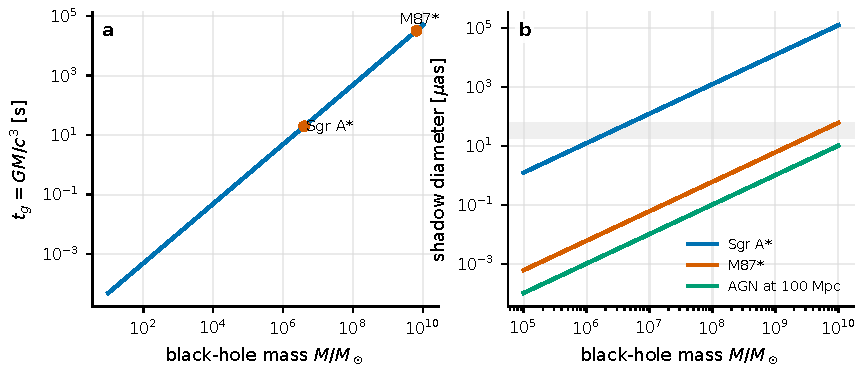
\includegraphics[width=0.94\linewidth]{figures/generated/chapter_12/ch12_black_hole_scales.pdf}
\caption{The time scale and angular scale of a black hole are both linearly controlled by the mass. The masses of Sgr~A* and M87* differ by about \(10^3\), but the distances also differ by about \(10^3\), so both shadow angular diameters are a few tens of microarcseconds; the time scales, however, are completely different: Sgr~A* can change within a single VLBI scan, while M87*'s structure is closer to static.}
\label{fig:e19-scales}
\end{figure}

With a ruler in hand, we can write the ``event-table coordinates'' of black-hole observation in full. In earlier chapters we recorded a photon detection as an arrival time and a frequency; for black-hole imaging, the coordinate expands to
\[
  (t_i,\ \nu_i,\ \bm{b}_i,\ \eta_i,\ w_i),
\]
where \(t_i\) is the arrival time, \(\nu_i\) is the frequency or energy channel, \(\bm{b}_i\) is the projected baseline (determining which spatial frequency is measured), \(\eta_i\) is the polarization channel, and \(w_i\) is the weight. The complex visibilities of the EHT, the differential phases of GRAVITY, and the light curves of optical monitoring can all be seen as different projections of this event table. The crux: retain the time and polarization as much as possible before projecting, so that accretion-flow variations, jet perturbations, and strong-gravity multipath can be estimated separately. This line of thought is the same language as ``from visibility to imaging'' in \ref{chap:e11}, only that the measured object is now light bent by strong gravity.

\section{How the Accretion Disk Produces a Continuum and Random Variability}
\label{sec:e19-disk}

The black hole does not glow; what glows is the gas falling toward it. The gas carries angular momentum, cannot fall straight in, and can only spiral inward ring by ring, rubbing against itself, grinding the gravitational potential energy into heat, and finally radiating it away: this is the accretion disk. The standard thin-disk model gives the radiant flux per unit area:
\begin{equation}
  F(R)=\frac{3GM\dot M}{8\pi R^3}
  \left[1-\left(\frac{R_{\rm in}}{R}\right)^{1/2}\right],
  \label{eq:e19-flux}
\end{equation}
\begin{formulaexplain}
\(F(R)\) is the power radiated outward per unit area at radius \(R\) on the disk, \(\dot M\) is the accretion rate, and \(R_{\rm in}\) is the inner boundary. The bracket makes the flux vanish at the inner boundary.
\end{formulaexplain}
Symbol by symbol: \(R\) is the disk radius (cm), \(\dot M\) is the accretion rate (\({\rm g\,s^{-1}}\)), and \(R_{\rm in}\) is the disk's inner boundary, usually taken as a few times \(r_g\) (for a non-spinning black hole the ISCO is at \(6r_g\)). The bracket \([\,1-(R_{\rm in}/R)^{1/2}\,]\) ensures that the matter has no net torque at the inner boundary and the flux tends to zero; once \(R\gg R_{\rm in}\), the bracket approaches 1 and the dominant behavior is \(F\propto R^{-3}\).

If the disk is locally approximately a blackbody, convert the flux into a temperature:
\begin{equation}
  T(R)=\left[\frac{F(R)}{\sigma_{\rm SB}}\right]^{1/4},
  \label{eq:e19-temp}
\end{equation}
\begin{formulaexplain}
\(T(R)\) is the local effective temperature of the disk at radius \(R\), and \(\sigma_{\rm SB}\) is the Stefan--Boltzmann constant. The color of the thin-disk spectrum is superposed from the blackbody temperatures at different radii.
\end{formulaexplain}
Far from the inner boundary \(F\propto R^{-3}\), and substituting and noting the fourth root:
\[
  T(R)\propto \big(R^{-3}\big)^{1/4}=R^{-3/4}
  \quad\Longrightarrow\quad
  T(R)\propto (M\dot M)^{1/4}\,R^{-3/4}.
\]
This is the thin disk's most famous temperature law: the farther in, the hotter, the bluer the color. Now ask a question an observer would ask: from which radius does a given wavelength \(\lambda\) mainly come? A blackbody is brightest at wavelength \(\lambda\) when the Wien relation \(k_{\rm B}T\sim hc/\lambda\) holds, i.e., \(T\propto1/\lambda\). Insert this condition into the temperature law:
\[
  \frac{1}{\lambda}\propto (M\dot M)^{1/4}R_\lambda^{-3/4}
  \;\Longrightarrow\;
  R_\lambda^{3/4}\propto (M\dot M)^{1/4}\lambda
  \;\Longrightarrow\;
  R_\lambda\propto (M\dot M)^{1/3}\lambda^{4/3}.
\]
Written as a scaling formula:
\begin{equation}
  R_\lambda \propto (M\dot M)^{1/3}\,\lambda^{4/3}.
  \label{eq:e19-Rlambda}
\end{equation}
\begin{formulaexplain}
\(R_\lambda\) is the disk radius that mainly glows near wavelength \(\lambda\). Longer wavelengths come from more outer layers; the larger the mass and accretion rate, the larger the glowing ring of the same color.
\end{formulaexplain}
This \(R_\lambda\propto\lambda^{4/3}\) is a ``fingerprint'' that can be observationally tested. For a quasar with \(M\sim10^8\,M_\odot\) and Eddington ratio \(L/L_{\rm Edd}\sim0.1\), the optical-to-near-ultraviolet continuum comes roughly from radii of order \(0.1\)--\(10\) light-days. Interestingly, microlensing and multiband delay measurements often give a larger optical disk than the simplest thin disk, which is exactly why the inhomogeneous-disk and reprocessing models are discussed again and again \citep{1973A&A....24..337S,2006ApJ...642...87P,2011ApJ...727L..24D}. The orange region on the left of Figure~\ref{fig:e19-disk} illustrates this case of ``the measured optical disk being larger.''

\begin{figure}[tbp]
\centering
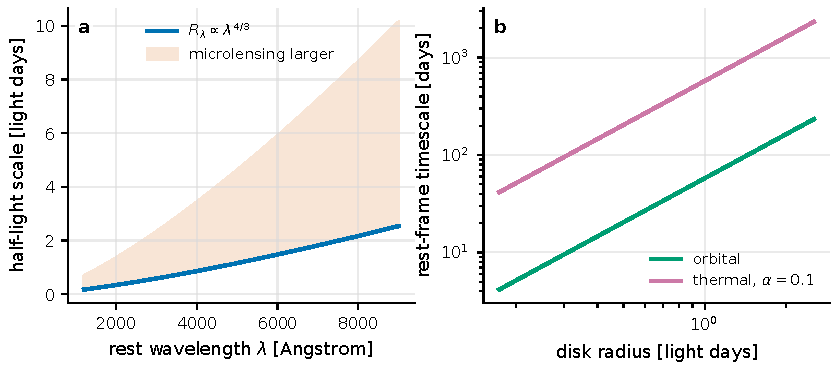
\includegraphics[width=0.94\linewidth]{figures/generated/chapter_12/ch12_accretion_disk_radii.pdf}
\caption{The thin-disk scaling gives \(R_\lambda\propto\lambda^{4/3}\). The left panel's orange region indicates the larger optical glowing area often suggested by microlensing and part of the continuum delays; the right panel compares the orbital time and thermal time at the same radius, and for \(\alpha\simeq0.1\) the thermal time is about ten times the orbital time.}
\label{fig:e19-disk}
\end{figure}

Glowing is a static picture, but the accretion disk is also constantly ``flickering.'' To understand the timescale of the variability, first estimate the two clocks at a radius on the disk:
\begin{equation}
  t_{\rm orb}=2\pi\left(\frac{R^3}{GM}\right)^{1/2},\qquad
  t_{\rm th}\simeq\frac{t_{\rm orb}}{\alpha}.
  \label{eq:e19-times}
\end{equation}
\begin{formulaexplain}
\(t_{\rm orb}\) is the Keplerian orbital period, \(t_{\rm th}\) is the thermal time (the time needed for the local stored energy to be rewritten by radiation), and \(\alpha\) is the viscosity parameter. Which clock a perturbation falls on determines how fast the variability can respond.
\end{formulaexplain}
\(t_{\rm orb}\) is just the orbital time obtained by taking the period \(2\pi/\Omega\) of Kepler's third law \(\Omega^2=GM/R^3\); \(t_{\rm th}\) is the thermal time, the time needed for the local stored heat to be redistributed by radiation. \(\alpha\) is the Shakura--Sunyaev viscosity parameter (dimensionless), usually taken as \(0.01\)--\(0.3\). Because \(\alpha<1\), the thermal time is always longer than the orbital time, and the right of Figure~\ref{fig:e19-disk} takes \(\alpha\simeq0.1\), differing by about a factor of ten. For an AGN optical disk, \(t_{\rm orb}\) can be tens of days to years, and \(t_{\rm th}\) is longer still: this is why quasar optical variability has a tempo of ``months to years.''

Large-sample optical variability is often described by the damped random walk (DRW), whose autocovariance and power spectrum are a pair:
\begin{equation}
  C(\tau)=\sigma^2\exp\!\left(-\frac{|\tau|}{\tau_d}\right),
  \qquad
  P(f)\propto\frac{1}{1+(2\pi f\tau_d)^2}.
  \label{eq:e19-drw}
\end{equation}
\begin{formulaexplain}
\(C(\tau)\) is the autocovariance of the variability, \(\tau_d\) is the damping (memory) time, and \(P(f)\) is the power spectrum. This model writes the random variability as a correlated process that ``slowly forgets itself.''
\end{formulaexplain}
Naming the symbols first: \(\sigma^2\) is the variance of the variability (the squared amplitude of the brightness fluctuation on long timescales), so \(\sigma\) has the same dimension as the measured brightness (or flux), the dimension of flux/magnitude; \(\tau\) is the time delay, and \(f\) is the frequency. Here the two equations are mutually Fourier transforms: the spectrum of an exponential autocovariance is Lorentzian (it is precisely with this pair of relations that we linked correlation time and bandwidth in \ref{chap:e02}). The physical picture is very plain: \(\tau_d\) is the time the disk ``remembers how bright it was a moment ago''; on timescales shorter than \(\tau_d\) the variability is highly correlated, and beyond it memory gradually fades, and the power spectrum turns into an \(f^{-2}\) decline at \(f\gtrsim1/2\pi\tau_d\). Observationally, \(\tau_d\) correlates with the black-hole mass, and supermassive black holes are often tens to hundreds of days (rest frame) \citep{1993ApJ...406..420M,2021Sci...373..789B,2016Natur.534...75M}. Figure~\ref{fig:e19-var} compares the memory behavior of short and long \(\tau_d\).

\begin{figure}[tbp]
\centering
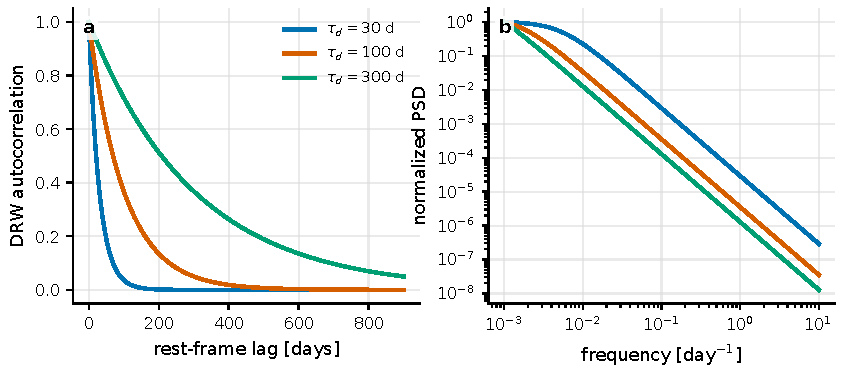
\includegraphics[width=0.94\linewidth]{figures/generated/chapter_12/ch12_variability_autocorrelation.pdf}
\caption{The damped random walk writes the random variability as a correlation time. Variability with short \(\tau_d\) loses memory quickly, and the power spectrum turns into an \(f^{-2}\) decline earlier; a disk with long \(\tau_d\) stays correlated over a longer time, and the low-frequency plateau extends farther.}
\label{fig:e19-var}
\end{figure}

Here we owe an honest reminder to readers interested in photon statistics. The \(g^{(2)}\) bunching of earlier chapters (\ref{chap:e08}) is the quantum fingerprint of single-mode thermal light; but the optical continuum of a \(10^8\,M_\odot\) AGN comes from an enormous number of mutually independent turbulent cells and the superposition of multiple thermal times, and is extremely multimode. Multimode averages away the bunching of each mode, and the measured \(g^{(2)}\) is compressed almost to 1. So the more realistic measurable on an accretion disk is not the raw bunching but the ``excess correlation'' under a phase or color condition: for example, comparing the change in the width of \(g^{(2)}(\tau)\) before and after a flare, or separating the polarization channels to read the lifetime of the turbulent cells. The mean brightness mainly gives the photon rate and the normalization; whether the correlation can truly be measured is further jointly constrained by the coherence time, the sampling window, and whether the classical fluctuations can be modeled.

\section{Strong Gravitational Lensing and the Geometric Origin of the Photon Ring}
\label{sec:e19-geometry}

Now we walk to the core picture of this chapter: how that bright ring comes about. The key is that light near a black hole does not travel in a straight line. Imagine you stand far away and shoot many light rays in parallel toward the black hole, each labeled by its impact parameter \(b\): \(b\) is ``how far the ray would graze past the black hole if there were no gravity.'' Gravity bends the rays inward:
\begin{itemize}
\item when \(b\) is large, the ray is only slightly deflected and flies straight past;
\item as \(b\) decreases, the deflection grows fiercer, and the ray begins to orbit the black hole for a small half-circle, one circle, a few circles;
\item there is a critical value \(b_c\): equal to it exactly, the ray asymptotically approaches some circular orbit and spirals endlessly; less than it, the ray plunges headlong into the black hole and never comes out again.
\end{itemize}
That circular orbit which lets light ``orbit'' is called the photon sphere. For a non-spinning (Schwarzschild) black hole, the photon-sphere radius and the critical impact parameter are standard general-relativity results:
\begin{equation}
  r_{\rm ph}=3\,\frac{GM}{c^2}=3\,r_g,\qquad
  b_c=3\sqrt{3}\,\frac{GM}{c^2}=3\sqrt{3}\,r_g\approx5.196\,r_g.
  \label{eq:e19-photonsphere}
\end{equation}
\begin{formulaexplain}
\(r_{\rm ph}\) is the radius at which a photon can move in a circle, and \(b_c\) is the critical impact parameter between escaping and being swallowed. They depend only on \(r_g\), that is, only on the mass.
\end{formulaexplain}
How to understand these two numbers? \(r_{\rm ph}=3r_g\) says the photon sphere sits just outside the Schwarzschild radius (\(2r_g\)), the place where ``light can just barely orbit but extremely unstably''; any tiny perturbation makes the orbiting light either fall inward or escape outward. \(b_c=3\sqrt3\,r_g\) is the dividing line on the sky: all the light from the background with impact parameter \(b<b_c\) has entered the black hole, so we see a dark patch; light with \(b\) slightly greater than \(b_c\) orbits several circles before escaping, stacking up on the outer edge of the dark patch into a thin bright ring. This ring is the photon ring.

The size of the dark patch can be computed directly. The shadow radius seen by the observer is precisely the critical impact parameter projected onto the sky as an angle, and the shadow angular diameter is
\begin{equation}
  d_{\rm sh}=\frac{2b_c}{D}=6\sqrt{3}\,\frac{r_g}{D}=6\sqrt{3}\,\theta_g\simeq10.4\,\theta_g,
  \label{eq:e19-shadow}
\end{equation}
\begin{formulaexplain}
\(d_{\rm sh}\) is the angular diameter of the black-hole shadow, equal to \(2b_c\) divided by the distance. The coefficient \(6\sqrt3\approx10.4\) is a purely geometric constant that magnifies the gravitational-radius angular scale by about ten times.
\end{formulaexplain}
This step cashes in the coefficient \(\kappa\simeq10.4\) planted in the previous section: it is not an empirical number fitted out but the geometric constant \(6\sqrt3\). For a rotating (Kerr) black hole, spin and inclination make the shadow slightly non-circular and the coefficient float within a few to a dozen-odd percent, but the order of magnitude is unchanged, so we can still safely use \(d_{\rm sh}\simeq10.4\,\theta_g\) for estimates.

Substituting the angular scale of the previous section gives the observable ring. M87* has \(\theta_g\simeq3.8\,\mu{\rm as}\), predicting \(d_{\rm sh}\simeq10.4\times3.8\simeq40\,\mu{\rm as}\); the EHT measured an asymmetric ring diameter of \(42\pm3\,\mu{\rm as}\) at \(1.3\,{\rm mm}\), with the central brightness suppressed by more than ten times, exactly the shadow. Sgr~A* has \(\theta_g\simeq4.9\,\mu{\rm as}\), predicting \(d_{\rm sh}\simeq51\,\mu{\rm as}\), and the measured thick-ring diameter is \(51.8\pm2.3\,\mu{\rm as}\), only that the source shows clear minute-to-hour variation within the observing night \citep{2019ApJ...875L...4E,2019ApJ...875L...5E,2022ApJ...930L..14E,2022ApJ...930L..15E}. A pure geometric constant \(6\sqrt3\) times a ruler fixed by the mass compresses the general-relativity prediction to two significant figures, in agreement with observation: this is the picture most worth remembering in this chapter.

To note: the bright ring the EHT sees is not the mathematically infinitely thin photon ring. It is several things stacked together: the direct radiation of the accretion flow itself, the ``first lensed image'' orbiting about half a circle, and the higher-order photon subrings orbiting many circles. The thickness, optical depth, turbulence, and time averaging of the accretion flow smear the narrow structure of strong gravity broad. The next section examines these layer-upon-layer nested subrings.

\section{The Self-Similar Subring Structure of the Photon Ring}
\label{sec:e19-subring}

The most fascinating property of the photon ring is that its interior hides a set of self-similar layered structures. Back to the geometric picture: the closer the impact parameter to the critical value \(b_c\), the more circles the light orbits the black hole before escaping. We number these images by ``number of half-circles orbited'' \(n=0,1,2,\dots\): \(n=0\) is the direct image that barely orbits, \(n=1\) is the first lensed image that orbits about half a circle and lands on the other side, and the larger \(n\), the more it orbits and the closer it hugs that critical curve. Each additional orbit makes the corresponding bright ring narrower, dimmer, and closer to the same limiting radius. Write the angular width and flux of the \(n\)-th subring in scaling form:
\begin{equation}
  w_n\simeq w_0\,e^{-\gamma n},\qquad
  F_n\simeq F_0\,e^{-\beta n}.
  \label{eq:e19-subring}
\end{equation}
\begin{formulaexplain}
\(w_n\) and \(F_n\) are the angular width and flux of the \(n\)-th photon subring. Both decay exponentially with \(n\): the subrings narrow and dim layer by layer and converge toward the critical curve.
\end{formulaexplain}
Here \(w_0,F_0\) are the width and flux scales of the outermost (low-order) structure, and \(\gamma\) and \(\beta\) are the decay exponents (dimensionless) controlling ``how much it shrinks per orbit.'' The exponent \(\gamma\) is set by the instability of the photon-sphere orbit: precisely the Lyapunov exponent of that extremely unstable circular orbit, characterizing the rate at which neighboring rays separate from each other during orbiting; \(\beta\) additionally depends on the emission and absorption along the way. Physically, \(w_n\sim e^{-\gamma n}\) means the subrings narrow by a nearly fixed ratio layer by layer, forming a self-similar ladder of ``rings within rings''; while \(F_n\sim e^{-\beta n}\) means that although the higher-order subrings become more and more universal in position (determined almost only by the Kerr metric, independent of accretion-flow details), their flux becomes smaller and smaller and harder and harder to measure.

The significance of this self-similar structure lies in its universality: the shape of the low-order images is polluted by the dirty details of the accretion flow, but the sufficiently high-order subrings remember almost only the spacetime geometry itself. Theory gives a very clean result for the Schwarzschild black hole: for each higher order, the position and width of the subring contract by an approximately fixed factor and the flux dims by an approximately fixed factor, converging onto the critical curve corresponding to \(b_c\) \citep{2019PhRvD.100b4018G,2020PhRvD.102l4004G,2020SciA....6.1310J}. Gralla et al. emphasize: in the total flux, the higher-order photon ring often occupies only a very small fraction, and separating them directly from the image is extremely difficult. This pushes the problem to the next section: if the image domain cannot see it clearly, can we switch to the visibility domain to see it.

\section{EHT Very-Long-Baseline Imaging and the Ring-Shaped Oscillation in the Visibility}
\label{sec:e19-visibility}

To resolve a ring of a few tens of microarcseconds, a single-aperture telescope has no hope: the diffraction limit \(\theta\sim\lambda/D_{\rm tel}\), and reaching \(20\,\mu{\rm as}\) at \(1.3\,{\rm mm}\) requires an aperture
\[
  D_{\rm tel}\sim\frac{\lambda}{\theta}
  =\frac{1.3\times10^{-3}\,{\rm m}}{20\,\mu{\rm as}}
  =\frac{1.3\times10^{-3}}{20\times4.848\times10^{-12}\,{\rm rad}}
  \approx1.3\times10^{7}\,{\rm m},
\]
that is, of order the Earth's diameter. This is exactly the reason very-long-baseline interferometry (VLBI) exists: connect telescopes distributed around the globe into one ``Earth-sized'' synthesis telescope. An interferometer does not give an image directly; it measures the Fourier components of the sky brightness distribution, the complex visibility:
\begin{equation}
  V(\bm{u})=\int I(\bm{\theta})\,
  e^{-2\pi i\,\bm{u}\cdot\bm{\theta}}\,d^2\theta,
  \qquad
  \bm{u}=\frac{\bm{B}_\perp}{\lambda}.
  \label{eq:e19-vis}
\end{equation}
\begin{formulaexplain}
\(V(\bm u)\) is the complex visibility, \(I(\bm\theta)\) is the sky brightness distribution, and \(\bm u=\bm B_\perp/\lambda\) is the projected baseline in units of wavelength (the spatial frequency). The longer the baseline, the higher the spatial frequency seen, and the finer the angular structure resolvable.
\end{formulaexplain}
This is the old friend of van~Cittert--Zernike and ``visibility is a Fourier component'' from \ref{chap:e10} and \ref{chap:e11}, only that the source is now a ring of light bent out by gravity. An idealized uniform thin ring has a beautiful analytic form for its visibility:
\begin{equation}
  V(u)\simeq J_0(\pi d\,u),
  \label{eq:e19-bessel}
\end{equation}
\begin{formulaexplain}
\(J_0\) is the zeroth-order Bessel function, \(d\) is the angular diameter of the ring, and \(u\) is the spatial frequency corresponding to the baseline length. The visibility of a thin ring oscillates with baseline and has nulls at a series of baselines.
\end{formulaexplain}
Why a Bessel function? For a thin ring of fixed radius, carrying out the Fourier integral around the ring, the azimuthal integral gives exactly \(J_0\): this is of the same geometric class as how the diffraction of a circular aperture gives a Bessel-type pattern. The point is: \(J_0(x)\) is an oscillating, decaying curve that crosses zero in turn at \(x=2.405,\,5.520,\dots\). So the fingerprint the ring leaves in the visibility is a string of \emph{nulls and sidelobes} appearing as the baseline lengthens: \(|V|^2\) shows a ring-shaped oscillation, rather than a monotonic decline like a smooth blob.

Work out which baseline the first null falls on, and you understand why the EHT is ``just barely enough.'' The first null is at \(\pi d\,u=2.405\), i.e.,
\[
  u_{\rm null}=\frac{2.405}{\pi d}=\frac{0.765}{d}.
\]
For M87*'s \(d\simeq42\,\mu{\rm as}=2.04\times10^{-10}\,{\rm rad}\):
\[
  u_{\rm null}=\frac{0.765}{2.04\times10^{-10}}\approx3.8\times10^{9}
  =3.8\,{\rm G}\lambda,
\]
converting to an actual baseline length \(B_\perp=u_{\rm null}\,\lambda=3.8\times10^9\times1.3\times10^{-3}\,{\rm m}\approx4.9\times10^{6}\,{\rm m}\), about \(5000\,{\rm km}\), far less than the Earth's diameter. That is to say, Earth-scale \(1.3\,{\rm mm}\) VLBI can just cross the first visibility trough and directly ``feel'' the ring structure in the visibility domain \citep{2019ApJ...875L...2E,2019ApJ...875L...3E,2020SciA....6.1310J}.

A real ring is not infinitely thin. If the ring has finite width \(w\), it is equivalent to multiplying the ideal \(J_0\) by an envelope whose width is inversely proportional to \(w\): wide structures are ``erased'' already at shorter baselines, and only narrow structures can keep oscillating at very long baselines. This connects the self-similar subrings of the previous section to the visibility domain; see Figure~\ref{fig:e19-ring}.

\begin{figure}[tbp]
\centering
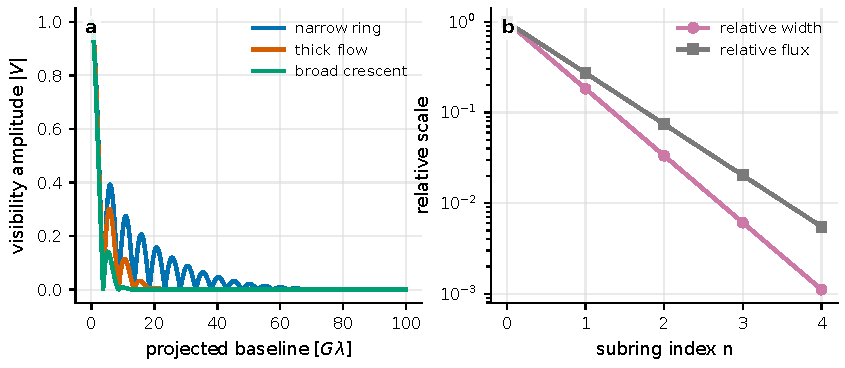
\includegraphics[width=0.94\linewidth]{figures/generated/chapter_12/ch12_photon_ring_visibility.pdf}
\caption{Ring-shaped structure produces oscillations in the long-baseline visibility. The left panel compares rings of different thickness at the same \(42\,\mu{\rm as}\) diameter; the narrow ring still retains oscillation at longer baselines. The right panel illustrates the width and flux of the photon subrings decreasing with the number of orbits; the higher-order subrings have small flux but can leave a universal oscillatory structure at sufficiently long baselines.}
\label{fig:e19-ring}
\end{figure}

This gives a beautiful strategy: in the image domain, the wide, bright accretion flow overwhelms the narrow, faint higher-order subrings; but in the visibility domain, as the baseline lengthens, the contribution of the wide accretion flow is first ``resolved out'' (its visibility decays below the noise early), and the remaining long-baseline signal is dominated more and more by the narrowest photon subring, exposing its universal oscillation determined almost only by the spacetime geometry \citep{2013ApJ...777..170J,2020SciA....6.1310J}. In other words, a sufficiently long baseline is a comb that can comb the universal structure of strong gravity out of the dirty background of the accretion flow.

\section{What Interference and Coherence Methods Can in Principle Add}
\label{sec:e19-coherence}

Connecting the tools of the first two parts, let us see what they can in principle add to our view of the black-hole edge structure. There are three core points.

\textbf{First, long baselines reveal the universal subrings.} As described in the previous section, the key resource of the visibility domain is the baseline length \(u=B_\perp/\lambda\). The baselines of the ground-based EHT are capped at the Earth's diameter, enough to see only the first and second visibility troughs; to dig out the ever-narrower, ever-more-universal oscillations of the \(n\ge2\)-th subrings, one must extend the baseline beyond the Earth (space VLBI) or shorten the wavelength. This is not new physics but pushing to the limit the principle of \ref{chap:e11}, ``longer baseline = higher spatial frequency = finer angular structure'': the self-similarity of the photon ring guarantees that, as long as the baseline is long enough, there is always a layer of subring waiting to be resolved.

\textbf{Second, the ring-shaped oscillation of \(|V|^2\) is itself a kind of coherence measurement.} Intensity interferometry (\ref{chap:e10}) measures precisely \(|V|^2\) (discarding the phase), and the ring's \(|V|^2\) is exactly a string of Bessel nulls and sidelobes, a ``ring-shaped fingerprint'' recognizable even without phase. This offers, for bright targets of larger angular scale, a channel that in principle does not depend on atmospheric phase stability and can use ultra-long baselines: as long as one can measure whether the \(|V|^2\) oscillation keeps time and where the nulls fall on a sufficiently long baseline, one can constrain the ring's diameter and width. The price is that the intensity-interferometry signal is weak and requires extremely high photon flux and long integration, so for most black-hole sources it remains in the near term a matter of principle rather than a ready-made practicality.

\textbf{Third, multipath leaves echoes in the temporal structure.} Light orbiting a different number of circles has a different path length and hence a different arrival time. If the mean delay difference between the \(n\)-th and \((n+1)\)-th circles is close to the photon orbital period \(T_\gamma\), then the intensity autocorrelation
\begin{equation}
  C(\tau)=\big\langle\delta I(t)\,\delta I(t+\tau)\big\rangle
  \quad\text{may at}\quad
  \tau\simeq m\,T_\gamma\ (m=1,2,\dots)
  \label{eq:e19-echo}
\end{equation}
\begin{formulaexplain}
\(C(\tau)\) is the autocorrelation of the intensity fluctuation, \(T_\gamma\) is the period of light orbiting the black hole once, and \(m\) is an integer. If the multipath contribution is visible, the autocorrelation will show faint echo peaks at these delays.
\end{formulaexplain}
show a faint peak nearby. The physical picture is: light from the same flicker, one part arriving directly and one part arriving later by \(T_\gamma\) after orbiting one more circle, forms an ``echo'' in the time series. For Sgr~A*, \(T_\gamma\) is of order minutes, overlapping exactly with the flare timescale of the accretion flow itself and easily confused; for M87*, \(T_\gamma\) is of order days, the source more stable but the observing scheduling harder. To truly interpret such a peak as strong-gravity multipath, one must first rule out jet shocks, disk turbulence, the scattering screen, the sampling window, and calibration errors: this is a high-threshold target, feasible in principle but demanding in practice. The polarization version can further compare the delay structure of the \(Q,U,V\) Stokes components, and the EHT's polarimetric imaging of M87* and Sgr~A* has already demonstrated the value of such information \citep{2021ApJ...910L..13E,2021PhRvD.104d4049G,2022PhRvD.106d3021C}.

We owe readers a faithful boundary. What these coherence methods can add is the \emph{angular and temporal structure of the edge}, not the black hole's own quantum radiation. The truly black-hole-intrinsic quantum process, Hawking radiation (\ref{chap:e16} will revisit it from the radiation-mechanism angle), has a temperature \(T_H\propto1/M\) already far below the \(2.725\,{\rm K}\) cosmic microwave background for stellar-mass black holes, and lower still to \(10^{-14}\)--\(10^{-17}\,{\rm K}\) for Sgr~A* and M87*, with an evaporation timescale far exceeding the age of the universe, beyond the sensitivity of any foreseeable telescope \citep{1974Natur.248...30H,1975CMaPh..43..199H}. So for astrophysical- and supermassive-mass black holes, the truly operable observational main line in the near term is still the four things covered in this chapter: accretion flow, polarization, visibility, and the temporal and angular structure of the photon ring.

\section{Chapter Summary}
\label{sec:e19-summary}

\begin{itemize}
\item \textbf{One ruler fixes the whole.} The length, time, and angular scale of a black hole are all proportional to the mass: \(r_g=1.477\,{\rm km}\,(M/M_\odot)\), \(t_g=4.93\,\mu{\rm s}\,(M/M_\odot)\), \(\theta_g=r_g/D\). The masses of Sgr~A* and M87* differ by \(10^3\) and the distances also by \(10^3\), so both shadows fall at a few tens of microarcseconds, but the time scales are one in seconds, the other in hours.
\item \textbf{The color and flicker of the accretion disk.} The thin-disk temperature law \(T\propto R^{-3/4}\) gives \(R_\lambda\propto(M\dot M)^{1/3}\lambda^{4/3}\): longer wavelengths come from more outer layers. The variability has a tempo of the orbital time and thermal time, summarizable by the correlation time \(\tau_d\) of a damped random walk. Multimode dilution smooths away the raw bunching.
\item \textbf{The geometric origin of the photon ring.} The photon sphere is at \(r_{\rm ph}=3r_g\), the critical impact parameter \(b_c=3\sqrt3\,r_g\). The shadow angular diameter \(d_{\rm sh}=6\sqrt3\,\theta_g\simeq10.4\,\theta_g\): the coefficient is a pure geometric constant that magnifies \(\theta_g\) by about ten times, and the prediction agrees with EHT measurements (M87* about \(42\,\mu{\rm as}\), Sgr~A* about \(52\,\mu{\rm as}\)) to two significant figures.
\item \textbf{Self-similar subrings.} The higher-order subring width \(w_n\sim e^{-\gamma n}\) and flux \(F_n\sim e^{-\beta n}\) narrow and dim layer by layer, converging onto the critical curve; \(\gamma\) is set by the Lyapunov exponent of the photon orbit, and the higher the order, the more universal and the harder to measure.
\item \textbf{The ring-shaped fingerprint in the visibility.} The thin-ring visibility \(V(u)\simeq J_0(\pi d u)\) oscillates and crosses zero over baseline, and the first null falls at about a \(5000\,{\rm km}\) baseline for M87*: Earth-scale VLBI can just cross it. A sufficiently long baseline can resolve out the wide accretion flow and expose the universal oscillation of the narrow subring.
\item \textbf{What coherence methods can add.} In principle there are three: longer baselines reveal higher-order universal subrings; the ring-shaped oscillation of \(|V|^2\) is a phase-independent coherence fingerprint; the intensity autocorrelation may show a multipath echo at \(\tau\simeq mT_\gamma\). What all three add is the edge structure, not Hawking radiation; the latter is far below the observable threshold for astrophysical black holes.
\end{itemize}

\noindent\textbf{Questions to Ponder.}
\begin{itemize}
\item If the observing wavelength is shortened from \(1.3\,{\rm mm}\) to \(0.87\,{\rm mm}\), how does the spatial frequency \(u=B_\perp/\lambda\) corresponding to the same ground-based baseline change? Is this favorable or unfavorable for resolving the photon-ring visibility oscillation?
\item The shadow coefficient \(6\sqrt3\) comes from Schwarzschild geometry. If the black hole spins fast, how do you expect the shadow to deviate from a perfect circle? Why can this chapter still safely use \(d_{\rm sh}\simeq10.4\,\theta_g\) for order-of-magnitude estimates?
\item For Sgr~A*, the photon orbital period \(T_\gamma\) is of order minutes, overlapping with the accretion-flow flare timescale. To attribute a faint peak in the intensity autocorrelation at \(\tau\simeq mT_\gamma\) to strong-gravity multipath, what control would you design to rule out the contribution of the accretion flow itself?
\end{itemize}

\chapter{Bursts, Transients, and Multi-Messenger Quantum Astronomy}
\label{chap:e20}

\begin{chapteropening}
Up to now we have mostly looked at ``steady'' objects: the angular diameter of a star, the coherence of an accretion disk, a signal we can slowly integrate for hours. But there is another half of the universe, one that does not grant you hours, only seconds, milliseconds, even nanoseconds. A thermonuclear explosion on the surface of a white dwarf, a fireball flung out by two merging neutron stars, a radio flash sweeping across the Earth: these are ``here and gone'' events. They compress an entire chain of physical processes onto a very short time axis, forcing us to answer the same question: \textbf{when the signal is fleeting, what exactly should we record, and how do we extract physical quantities from a mere handful of photons?}

The through-line of this chapter is as follows. First we make clear why, when facing a transient, the ``event table'' of Chapter~\ref{chap:e13} (each photon carrying a time, frequency, and polarization label) is worth far more than a smooth light curve. Then we treat triggering as an act of statistical inference, not ``sound the alarm the moment you see a bright spot.'' Next we return to the book's home turf: the photon statistics and coherence of transient sources. Finally we step into the multi-messenger era, watching how the three messengers of gravitational waves, neutrinos, and photons are stitched by \textbf{time} into a single physical event. Along the way we use expanding novae, kilonovae, gamma-ray burst afterglows, and tidal disruption events as four real worked examples.
\end{chapteropening}

\section{The fast-changing universe: why we keep a time tag on every photon}
\label{sec:e20-fast}

Let us set the scene. A \textbf{light curve} is a line obtained by binning photons in time, counting the number in each bin, and connecting them. It is intuitive, but it does something irreversible: it smears a detail like ``a 512\,nm photon arrived at second 3.417\,922'' into ``the bin at second 3.4 contains 217 photons.'' For a star that slowly brightens, no harm is done; but for a transient, the temporal structure is itself the physics.

In the prompt emission of a gamma-ray burst (GRB), the light can fluctuate violently on scales of \(10^{-2}\,\mathrm{s}\); the main pulse of a fast radio burst (FRB) is often only a millisecond wide, with sub-millisecond fine structure inside it; and each pulse of a pulsar arrives with clocklike precision on a millisecond period. Once these structures are averaged away by coarse binning, they can never be recovered. This is why Chapter~\ref{chap:e13} insists on writing every photon candidate as a row in the event table, preserving its arrival time \(t\), frequency/energy channel, and polarization channel, rather than storing only a curve. This is not fastidiousness: it is because the likelihood below loses no information only when it is \textbf{unbinned}.

Denote the \textbf{instantaneous arrival rate} of photons in a given detection channel by \(\lambda(t)\), in units of \(\mathrm{s^{-1}}\). Chapter~\ref{chap:e03} explained that over an extremely short interval the probability of a photon appearing is proportional to the rate times the duration, and independent of the others; this is an \textbf{inhomogeneous Poisson point process}. Chapter~\ref{chap:e14} already derived its log-likelihood step by step, by ``slicing time into infinitely narrow cells and taking \(\Delta t\to0\)''; here we simply invoke and use that result:
\begin{equation}
  \ln L=\sum_{j=1}^{N}\ln \lambda(t_j)-\int_{t_{\rm min}}^{t_{\rm max}}\lambda(t)\,dt .
  \label{eq:e20-poisson-likelihood}
\end{equation}
\begin{formulaexplain}
\(\ln L\) is the log-likelihood of the event table under an inhomogeneous Poisson process. The first term scores the model rate at \textbf{each actual photon arrival time} \(t_j\), adding credit where a photon lands in a high-rate region; the second term subtracts the \textbf{total photon number} predicted by the model over the whole window. The two pull against each other, so a model that ``only spikes at the events'' cannot cheat.
\end{formulaexplain}
Symbol by symbol: \(N\) is the number of photons in the window \([t_{\rm min},t_{\rm max}]\) (a dimensionless count), \(\{t_j\}\) are their arrival times (in s), and \(\lambda(t)\) is the rate model (in \(\mathrm{s^{-1}}\)). The pedagogical point of this expression lies in its ``balance structure'': the first term rewards the model for placing rate where photons actually appear, while the second penalizes the model for raising the rate where there are no photons: try to bluff, and one of the two terms will dock your score.

Why insist on unbinned data? Imagine a burst that rises extremely fast; the information about \(t_0\) (the onset time) may be carried by just the earliest three to five photons. If you first bin the data into \(0.1\,\mathrm{s}\) bins, those few photons get averaged together with the rest of the bin into a single number, and the sharp information about the onset evaporates on the spot. Equation~\eqref{eq:e20-poisson-likelihood} eats the raw times \(t_j\) directly, so it can squeeze out what a binned curve cannot. This is also why the chapter repeatedly stresses ``keep the time tag in the event table.''

One of the most commonly used rate models is a ``fast-rise, slow-decay'' trigger window:
\begin{equation}
  \lambda(t)=b+A\exp\!\left[-\frac{t-t_0}{\tau}\right]H(t-t_0),
  \label{eq:e20-exponential-rate}
\end{equation}
\begin{formulaexplain}
\(\lambda(t)\) is a fast-rise, slow-decay rate model: \(b\) is the background rate, \(A\) is the excess rate at the instant of the burst, \(t_0\) is the physical onset time, \(\tau\) is the decay timescale, and \(H\) is the step function (ensuring this term is absent before \(t_0\)).
\end{formulaexplain}
Here \(b\) and \(A\) are both in \(\mathrm{s^{-1}}\), while \(t_0\), \(\tau\), and \(t\) are in s, and \(H(x)\) is the Heaviside step function (0 for \(x<0\), 1 for \(x\ge0\), dimensionless). To let the reader feel that the formula describes a real observation, let us compute the integral of its second term: over the window \(t>t_0\),
\[
  \int_{t_0}^{t_{\rm max}}\!\Big(b+Ae^{-(t-t_0)/\tau}\Big)\,dt
  = b\,(t_{\rm max}-t_0)+A\tau\Big(1-e^{-(t_{\rm max}-t_0)/\tau}\Big).
\]
When \(t_{\rm max}-t_0\gg\tau\), the exponential term goes to 0, and the total photon number contributed by the source is about \(A\tau\), that is, ``peak rate times decay timescale,'' a very intuitive quantity. The \(\tau\) of a GRB prompt can be as short as \(10^{-2}\,\mathrm{s}\), the effective decay timescale of an optical afterglow is hours to days, and the \(\tau\) of novae and tidal disruption events can be as long as tens or even hundreds of days. The same formula spans more than four orders of magnitude in timescale, which is precisely the breadth of the word ``transient.''

\section{Triggering is an act of statistical inference, not ``sound the alarm the moment you see a bright spot''}
\label{sec:e20-trigger}

Transient observation begins with a trigger, but the trigger is itself already a judgment: ``the handful of photons I see, are they a new burst, or a background fluctuation?'' To get it right, we must start from a more general rate model. For the \(k\)-th detection channel, the event rate is the background plus the instrument's response to the source flux:
\begin{equation}
  \lambda_k(t)=b_k(t)+A_{{\rm eff},k}(t)
  \int R_k(\nu,p,t)\,F_\nu(t,p)\,d\nu ,
  \label{eq:e20-rate-response}
\end{equation}
\begin{formulaexplain}
\(\lambda_k\) is the rate of the \(k\)-th channel, \(b_k\) is the background, \(A_{{\rm eff},k}\) is the effective area, \(R_k\) is the instrument response (encompassing bandwidth, quantum efficiency, polarization selection, and time response), and \(F_\nu\) is the source's photon flux at frequency \(\nu\) and polarization \(p\). The observed rate is the result of the ``source'' passing through the ``instrument'' and then having the ``background'' added on top.
\end{formulaexplain}
As for units: \(\lambda_k\) is in \(\mathrm{s^{-1}}\), \(b_k\) is in \(\mathrm{s^{-1}}\) (the sum of airglow, host galaxy, dark counts, and false triggers), \(A_{{\rm eff},k}\) is the effective area (\(\mathrm{cm^2}\)), \(R_k\) is a dimensionless response weight, and \(F_\nu\) is the photon flux per unit area per unit frequency (\(\mathrm{cm^{-2}\,s^{-1}\,Hz^{-1}}\)). The single-channel rate of an optical transient can range from less than \(1\,\mathrm{s^{-1}}\) all the way to \(10^6\,\mathrm{s^{-1}}\); high-energy detectors often record in coarser energy channels, while fast radio and optical detectors strive to push their time stamps down to sub-microsecond or even nanosecond precision. Equation~\eqref{eq:e20-rate-response} is the ``detailed instrumental version'' of the ``\(b+A\cdots\)'' in Equation~\eqref{eq:e20-exponential-rate}: only by separating the ``source'' from the ``instrument'' can one compare results across different telescopes.

The trigger must choose a side between two hypotheses: the transient model \(M_{\rm tr}\) (``there really is a burst'') and the background model \(M_{\rm bg}\) (``it is only background''). The language of estimation from Chapter~\ref{chap:e12} tells us that the right referee is the \textbf{odds ratio}:
\begin{equation}
  {\cal O}_{\rm tr,bg}
  =
  \frac{P(M_{\rm tr})}{P(M_{\rm bg})}
  \frac{L(D\mid M_{\rm tr})}{L(D\mid M_{\rm bg})},
  \label{eq:e20-trigger-odds}
\end{equation}
\begin{formulaexplain}
\({\cal O}_{\rm tr,bg}\) is the odds ratio of the transient model relative to the background model. It is a product of two pieces: on the left is the ratio of \textbf{prior rates} (how rare such a burst is to begin with), and on the right is the ratio of \textbf{data likelihoods} (which model the data resemble more).
\end{formulaexplain}
Here \(D\) is the event table or image-difference data, \(P(M)\) is the prior probability of the model (dimensionless), and \(L(D\mid M)\) is a likelihood like Equation~\eqref{eq:e20-poisson-likelihood}. This expression turns a piece of common sense into mathematics: the rarer the burst, the stronger the data must be before you dare to raise an alarm. Ignoring the prior ratio on the left is at the root of many ``false alarms flying everywhere.''

Beyond the prior, we also need a computable \textbf{false alarm probability}. If the expected background count within a time window \(\Delta t\) is \(\mu_b=b\,\Delta t\), then the probability that ``the background alone produces \(n\) or more photons'' is the tail of a Poisson distribution:
\begin{equation}
  P_{\rm FA}(N\ge n)=
  \sum_{m=n}^{\infty}\frac{\mu_b^m e^{-\mu_b}}{m!}.
  \label{eq:e20-false-alarm}
\end{equation}
\begin{formulaexplain}
\(P_{\rm FA}\) is the probability that the background alone produces \(n\) or more photons, and \(\mu_b=b\,\Delta t\) is the expected background count. Setting a trigger threshold is essentially drawing a red line across this Poisson tail probability.
\end{formulaexplain}
Let us plug in numbers to get a feel: if the background rate is \(b=1\,\mathrm{s^{-1}}\) and the window is \(\Delta t=0.1\,\mathrm{s}\), then \(\mu_b=0.1\). The probability that the background happens to throw up \(n\ge5\) photons is \(\sum_{m\ge5}0.1^m e^{-0.1}/m!\approx 8\times10^{-8}\), which sounds safe enough. But in reality you are not looking at just one window: a survey searches repeatedly over thousands of time windows, millions of sky pixels, dozens of energy channels, and dozens of templates. The true number of false triggers must be \textbf{multiplied by the number of trials} (the trials factor). If there are \(10^{10}\) effectively independent trials in one night, then that \(8\times10^{-8}\) above means about \(800\) false alarms. This is why FRB searches, gamma-ray triggers, and optical difference surveys, despite their \(\Delta t\) ranging from milliseconds to days and their backgrounds ranging from instrumental noise to variable-star contamination, all wrestle with the same ``trials factor'' ghost \citep{2013Sci...341...53T,2017ApJ...835...29Y,2020Natur.587...59B,2020Natur.587...54C,2020Natur.581..391M}.

\begin{figure}[tbp]
\centering
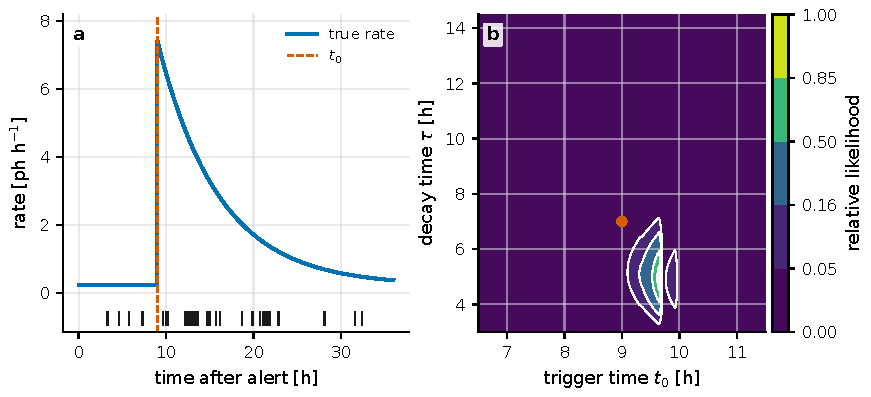
\includegraphics[width=0.92\linewidth]{figures/generated/chapter_13/ch13_transient_event_likelihood.pdf}
\caption{How an inhomogeneous Poisson event table constrains the trigger time and decay time. In the left panel each vertical line is one photon's arrival time and the blue curve is the rate model \(\lambda(t)\); the right panel writes the same event table as a relative likelihood surface over \(t_0\) and \(\tau\). A few early photons \textbf{strongly} pin down \(t_0\), while the late-time background determines whether \(\tau\) is overestimated. This is precisely the ``one reward, one penalty'' pair of terms in Equation~\eqref{eq:e20-poisson-likelihood} at work.}
\label{fig:e20-event-likelihood}
\end{figure}

\section{The photon statistics and coherence of transient sources}
\label{sec:e20-coherence}

Now back to the book's home turf: photon statistics. What kind of light does a transient source actually emit? This determines whether we can apply the coherence functions of Chapter~\ref{chap:e08} or the intensity interferometry of Chapter~\ref{chap:e10} to it.

The ``continuum face'' of the vast majority of transients is \textbf{thermal and chaotic}: the early spectra of novae, supernovae, kilonovae, and tidal disruption events can all be approximated by a blackbody photosphere (see Equation~\eqref{eq:e20-kilonova-blackbody} below). For such light, Chapter~\ref{chap:e08} gave the Siegert relation
\[
  g^{(2)}(\tau)=1+\zeta\,|g^{(1)}(\tau)|^2,
\]
that is, the photons ``pile up'' (bunch) within the coherence time. And the coherence time is set by the bandwidth; Chapter~\ref{chap:e02} gave \(\tau_c\simeq 1/\Delta\nu\). Here is an order-of-magnitude fact that is extremely real for transient observation: for a broadband optical photosphere, \(\Delta\nu\) is readily of order \(10^{13}\,\mathrm{Hz}\), so \(\tau_c\sim10^{-13}\,\mathrm{s}\), only a hundred femtoseconds. In other words, photon bunching happens on \textbf{femtosecond} scales, whereas the time bin you use to draw a light curve is a millisecond. Within a millisecond bin, the bunching has long been averaged clean, and the counting statistics degenerate into pure Poisson: the fluctuation in each bin is just the \(\sqrt N\) shot noise (Chapter~\ref{chap:e03}).

This conclusion has two faces. One is reassuring: when doing transient \textbf{photometry}, it suffices to treat the counts with Poisson errors, and the whole inference of Equation~\eqref{eq:e20-poisson-likelihood} is self-consistent. The other is a reminder: the coherence information of a thermal transient is hidden on femtosecond scales, and only \textbf{intensity interferometry} pushing time resolution to the nanosecond or even picosecond level can touch it. And the statistical precision of intensity interferometry is set by the number of \textbf{photon pairs} accumulated within the correlation window:
\begin{equation}
  N_{\rm pair}\simeq r_1 r_2\,\Delta t\,T,
  \qquad
  \delta C\simeq N_{\rm pair}^{-1/2},
  \label{eq:e20-pair-statistics}
\end{equation}
\begin{formulaexplain}
\(N_{\rm pair}\) is the number of photon pairs accumulated by two telescopes (rates \(r_1,r_2\)) within a correlation window \(\Delta t\) over a total integration time \(T\); \(\delta C\) is the correlation measurement error under pure Poisson statistics, which falls as the square root of the number of pairs.
\end{formulaexplain}
Here \(r_1,r_2\) are the event rates of the two stations (\(\mathrm{s^{-1}}\)), \(\Delta t\) is the correlation time window (s), \(T\) is the accumulated time (s), and \(N_{\rm pair}\) is dimensionless. Substituting a set of real numbers: \(r_1=r_2=10^6\,\mathrm{s^{-1}}\), \(\Delta t=100\,\mathrm{ps}=10^{-10}\,\mathrm{s}\), \(T=1\,\mathrm{h}=3600\,\mathrm{s}\), then
\[
  N_{\rm pair}\simeq (10^6)(10^6)(10^{-10})(3600)=3.6\times10^{5},
  \qquad
  \delta C\simeq (3.6\times10^5)^{-1/2}\approx1.7\times10^{-3}.
\]
That is, in one hour the correlation can be measured to the level of one part in a thousand, but note that this is only the \textbf{statistical floor}. The true error must also add on timing-synchronization error, dead time, spectral bandwidth, polarization leakage, and background fluctuations. For a fleeting source, \(T\) itself is capped by the lifetime of the burst, and this formula immediately tells you whether ``you can accumulate enough pairs before the source vanishes'', a hard constraint.

There is also a small class of transients that emit not thermal light at all but \textbf{coherent emission}: the radio pulses of FRBs and pulsars are the representatives. The criterion is the \textbf{brightness temperature} \(T_b\), the temperature that would be required ``if it were thermal radiation,'' obtained by converting the observed brightness via the Rayleigh--Jeans law. In the radio band, the photon energy is far below the thermal energy (\(h\nu\ll k_{\rm B}T_b\)), and the single-mode occupation number used in Chapters~\ref{chap:e05} and \ref{chap:e16} degenerates into a large number:
\[
  \bar n_\nu=\big[\exp(h\nu/k_{\rm B}T_b)-1\big]^{-1}
  \;\xrightarrow[h\nu\ll k_{\rm B}T_b]{}\;
  \frac{k_{\rm B}T_b}{h\nu}\gg1 .
\]
Here we have used the standard Taylor expansion \(e^x-1\approx x\) (as \(x\to0\)), setting \(x=h\nu/k_{\rm B}T_b\). So ``the radio occupation number is large'' is in itself no surprise: \(k_{\rm B}/h\approx2.08\times10^{10}\,\mathrm{Hz\,K^{-1}}\), so as long as \(T_b\gg h\nu/k_{\rm B}\) (only \(0.05\,\mathrm{K}\) at \(\nu=1\,\mathrm{GHz}\)), almost all thermal radio sources fall in the classical high-occupation regime \(\bar n_\nu\gg1\) (at \(\nu=1\,\mathrm{GHz}\), \(T_b=10^4\,\mathrm{K}\), \(\bar n_\nu\sim2\times10^5\)). Evidently the size of the occupation number is not a clean criterion. The real criterion is whether the brightness temperature \textbf{has an upper limit}: the \(T_b\) of any \textbf{incoherent} radiation mechanism is capped at order \(T_b\sim10^{12}\,\mathrm{K}\) by the \textbf{inverse Compton catastrophe}: any brighter and the relativistic electrons would be repeatedly inverse-Compton-scattered by the very synchrotron photons they just emitted, dissipating their energy in an extremely short time so that the brightness cannot climb. Yet the brightness temperatures inferred for FRBs from the observed flux, millisecond timescales, and source distance reach as high as \(T_b\sim10^{35\text{--}40}\,\mathrm{K}\), more than twenty orders of magnitude above this upper limit; the corresponding \(\bar n_\nu\propto T_b\) also far exceeds anything an incoherent process could reach. This can only mean that a large number of charges radiate together in the same phase, a coherent process like a laser or maser, not each independent particle radiating on its own. For such a source, ``photon bunching'' is no longer a weak effect but the emission mechanism itself. Identifying it, and distinguishing it from the background and from instrumental artifacts, likewise relies only on the sub-millisecond time and polarization labels in the event table \citep{2020Natur.587...59B,2020Natur.587...54C,2020Natur.581..391M}.

\section{The expanding fireball: linking speed, time, and angular scale into a cosmic ruler}
\label{sec:e20-expansion}

Many transients (novae, supernovae, kilonovae) are physically the same picture: a cloud of \textbf{ejecta expanding in velocity layers}. The outer layers are fast and the inner layers slow; the early photosphere sits in the outermost optically thick layer and recedes inward with time. If the expansion is approximately \textbf{homologous} (self-similar), i.e.\ radius and velocity satisfy \(r=v(t-t_0)\), then the angular radius it subtends ties ``speed, time, and distance'' together:
\begin{equation}
  \theta(t)=\frac{v_{\rm exp}(t-t_0)}{D}
  =
  5.8\,{\rm mas}
  \left(\frac{v_{\rm exp}}{10^8\,{\rm cm\,s^{-1}}}\right)
  \left(\frac{t-t_0}{10\,{\rm d}}\right)
  \left(\frac{D}{1\,{\rm kpc}}\right)^{-1}.
  \label{eq:e20-angular-expansion}
\end{equation}
\begin{formulaexplain}
\(\theta(t)\) is the angular radius of the expanding source, \(v_{\rm exp}\) is the expansion velocity, \(D\) is the distance, and \(t_0\) is the burst time. The physics is plain: how far the material has traveled (\(v_{\rm exp}(t-t_0)\)), divided by how far it is from us (\(D\)), is the angle it subtends.
\end{formulaexplain}
Let us compute that \(5.8\,\mathrm{mas}\) coefficient for you, rather than let it appear from nowhere: take \(v_{\rm exp}=10^8\,\mathrm{cm\,s^{-1}}\), \(t-t_0=10\,\mathrm{d}=8.64\times10^5\,\mathrm{s}\), so the linear radius is \(v_{\rm exp}(t-t_0)=8.64\times10^{13}\,\mathrm{cm}\); the distance is \(D=1\,\mathrm{kpc}=3.086\times10^{21}\,\mathrm{cm}\). Dividing gives \(\theta=2.80\times10^{-8}\,\mathrm{rad}\). Then converting with \(1\,\mathrm{rad}=2.063\times10^{8}\,\mathrm{mas}\): \(\theta=2.80\times10^{-8}\times2.063\times10^{8}\approx5.8\,\mathrm{mas}\). The orders of magnitude then fall into place: a Galactic nova (\(D\sim1\text{--}5\,\mathrm{kpc}\), \(v_{\rm exp}\sim10^8\,\mathrm{cm\,s^{-1}}\)) can climb to the milliarcsecond level in a few to a few tens of days; whereas a Type Ia supernova, though its \(v_{\rm exp}\sim10^9\,\mathrm{cm\,s^{-1}}\) is ten times faster, has a ten-day angular radius of only a few microarcseconds because it sits \(10\text{--}100\,\mathrm{Mpc}\) away; and a GW170817-type kilonova, with speeds as high as \(0.1\text{--}0.3c\), is nonetheless compressed by its \(40\,\mathrm{Mpc}\) distance to below a microarcsecond in early angular scale.

\begin{figure}[tbp]
\centering
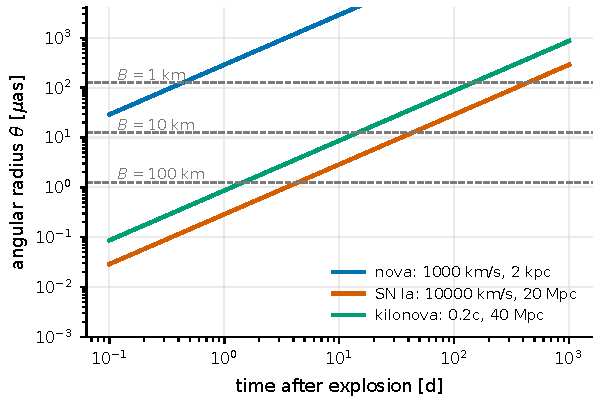
\includegraphics[width=0.92\linewidth]{figures/generated/chapter_13/ch13_expanding_fireball_resolution.pdf}
\caption{The angular radius of an expanding source is jointly determined by speed, time, and distance. A Galactic nova, though low in speed, wins by being nearby and enters the milliarcsecond regime fastest; low-redshift Type Ia supernovae and kilonovae are higher in speed but fall in the microarcsecond regime because they are too far away. The horizontal dashed lines are the \(\lambda/B\) resolution scales of different optical baselines at \(\lambda=0.5\,\mu\mathrm{m}\), they mark the threshold of ``who can be resolved by existing interferometers.''}
\label{fig:e20-expansion}
\end{figure}

Where does the \(v_{\rm exp}\) in Equation~\eqref{eq:e20-angular-expansion} come from? From spectral lines. A spectral line projects the line-of-sight velocity onto wavelength:
\begin{equation}
  v_{\rm los}\simeq c\,\frac{\lambda_{\rm obs}-\lambda_0}{\lambda_0},
  \label{eq:e20-doppler-line}
\end{equation}
\begin{formulaexplain}
\(v_{\rm los}\) is the line-of-sight velocity, \(\lambda_0\) is the laboratory wavelength, and \(\lambda_{\rm obs}\) is the observed wavelength. How far the line has shifted relative to its laboratory position ``imprints'' the velocity layer of the ejecta onto the wavelength axis.
\end{formulaexplain}
Here \(v_{\rm los}\) and \(c\) share the same units (\(\mathrm{cm\,s^{-1}}\)), and \(\lambda\) is the wavelength (cm or \(\text{\AA}\)). One must be careful: the blue edge of a P-Cygni absorption often represents the \textbf{fastest, outermost} material, the absorption minimum is closer to the layer of maximum optical depth, and the half-width of an emission line mixes several effects: geometry, optical depth, and density distribution. If one could measure the angular scale in each spectral-line channel, the data would become a set of \(\theta(v_{\rm los})\), which can distinguish a spherical shell, a bicone, an equatorial ring, or a polar wind.

How does one ``measure'' the angular scale? In intensity interferometry, the second-order correlation of a circularly symmetric uniform disk gives the squared visibility amplitude \(|V|^2\), whose first-order visibility modulus is the familiar Airy form (Chapter~\ref{chap:e11}):
\begin{equation}
  |V(B)|=
  \left|
  \frac{2J_1(\pi B\Theta/\lambda)}{\pi B\Theta/\lambda}
  \right|,
  \label{eq:e20-uniform-disk-visibility}
\end{equation}
\begin{formulaexplain}
\(|V(B)|\) is the visibility modulus of a uniform disk, \(\Theta=2\theta\) is the angular diameter, \(B\) is the projected baseline, \(\lambda\) is the wavelength, and \(J_1\) is the first-order Bessel function. The longer the baseline and the larger the source, the faster the visibility drops: this is precisely the quantitative meaning of ``resolving.''
\end{formulaexplain}
In this expression \(J_1\) is the first-order Bessel function (this is the standard result for circular-aperture diffraction, with its first zero at argument \(3.83\)), \(\Theta\) is the angular diameter (rad), \(B\) is the baseline (cm), and \(\lambda\) is the wavelength (cm). It assumes circular symmetry, a single wavelength, and no strong limb darkening; real novae and supernovae often require thin-shell, ring, ellipsoidal, or multi-component models. Combining the angular-expansion Equation~\eqref{eq:e20-angular-expansion} with the spectral-line velocity Equation~\eqref{eq:e20-doppler-line} yields a cosmic ruler independent of standard candles, the \textbf{expansion parallax}:
\begin{equation}
  D=\frac{v_{\rm exp}(t-t_0)}{\theta(t)}.
  \label{eq:e20-expansion-parallax}
\end{equation}
\begin{formulaexplain}
\(D\) is the geometric distance: the linear velocity times the time gives the linear radius, divided by the measured angular radius \(\theta(t)\) gives the distance. Its prerequisite is that \(v_{\rm exp}\) and \(\theta\) must correspond to the \textbf{same material layer}.
\end{formulaexplain}
This is a simple inversion of Equation~\eqref{eq:e20-angular-expansion}, but that prerequisite is where all the risk lies: if the spectral line measures the fast absorption of the outer layer while the angular scale comes from the continuum photosphere (which is more interior and slower), you are comparing two different velocity layers, and the distance will be systematically biased. A classical nova is itself a thermonuclear explosion on the surface of a white dwarf, with ejected mass \(10^{-5}\text{--}10^{-4}M_\odot\) and speeds exceeding \(10^3\,\mathrm{km\,s^{-1}}\); ever since Fermi discovered that novae are GeV \(\gamma\)-ray sources, the physical picture has been rewritten into a two-flow structure: a slow, dense equatorial ejection shaped by the binary orbit, struck by a fast polar wind that accelerates particles in the internal shock. The \(\gamma\)-ray emission of V959\,Mon lasted about \(12\,\mathrm{d}\), and high-resolution radio imaging showed the shock located exactly at the interface between the polar flow and the equatorial material, with a thermal ejecta mass of about \(4\times10^{-5}M_\odot\), in such a source \(v_{\rm exp}\) inherently contains two velocity components, and the spectral lines, radio images, and photon event table must be fit jointly \citep{2014Natur.514..339C,2014Sci...345..554A}.

Type Ia supernovae take another road: first they are calibrated into standard candles using the light-curve width. The Phillips relation corrects the peak absolute magnitude using the \(B\)-band decline rate \(\Delta m_{15}(B)\), and cosmological applications then write the corrected distance modulus as
\begin{equation}
  \mu = m_B - M_B + \alpha x_1-\beta C+\Delta_{\rm host},
  \label{eq:e20-snia-distance-modulus}
\end{equation}
\begin{formulaexplain}
\(\mu\) is the distance modulus, \(m_B,M_B\) are the observed and standardized peak magnitudes, \(x_1\) is the light-curve width, \(C\) is the color, and \(\alpha,\beta,\Delta_{\rm host}\) are fit from the sample. Standardizing a Type Ia is essentially correcting the luminosity a little at a time.
\end{formulaexplain}
Here \(m_B,M_B\) are magnitudes (dimensionless), \(x_1,C\) are dimensionless, and \(\Delta_{\rm host}\) is a host-galaxy-related correction term. A nearby Type Ia sample with \(m_B\sim10\text{--}16\) can yield high signal-to-noise light curves with a small telescope, while cosmological samples are often at \(m_B\sim22\text{--}25\). If one day one could \textbf{simultaneously} measure the angular expansion, one could use the geometric distance of Equation~\eqref{eq:e20-expansion-parallax} to cross-check this luminosity distance, which is very hard, because the ten-day Type Ia angular diameter is only of order microarcseconds, making it, in long-baseline optical intensity interferometry, a target of ``extreme difficulty but clear payoff'' \citep{1993ApJ...413L.105P,1998AJ....116.1009R,1999ApJ...517..565P}.

Is the ejecta round or not? Look at the polarization. The normalized Stokes parameters give the degree of linear polarization:
\begin{equation}
  q=\frac{Q}{I},\qquad
  u=\frac{U}{I},\qquad
  P=\sqrt{q^2+u^2},
  \label{eq:e20-stokes-polarization}
\end{equation}
\begin{formulaexplain}
\(q,u\) are the Stokes parameters normalized by the total intensity \(I\), and \(P\) is the degree of linear polarization. If the ejecta is perfectly spherically symmetric, the scattering cancels in all directions and \(P\to0\); once \(P\neq0\) appears, it signals a non-spherically-symmetric geometry.
\end{formulaexplain}
\(q,u,P\) are all dimensionless, usually reported as percentages. SN\,1999by near maximum had \(P\simeq0.3\text{--}0.8\%\), with an additional polarization variation of about \(0.4\%\) near Si\,II\,\(6150\,\text{\AA}\); models point to an overall asphericity of about \(20\%\), with the silicon layer and the continuum sharing broadly the same symmetry axis \citep{2001ApJ...556..302H}. So \(\theta(t)\) (from the photosphere shape), \(v_{\rm exp}\) (from the velocity layers), and \(P(t,\lambda)\) (from the scattering geometry) should all be interpreted within the same geometric model. This is precisely how ``keeping the frequency and polarization labels'' pays off for this class of source.

Finally there is the earliest, fastest window of a supernova, the \textbf{shock breakout}. When the shock is still at some depth \(d\) below the surface, radiation diffuses out first and forms a precursor. Let the local density be \(\rho\), the \textbf{opacity} \(\kappa\) (in units \(\mathrm{cm^2\,g^{-1}}\), about \(0.2\text{--}0.4\) for electron scattering, reaching order ten when heavy elements are present), so that the optical depth is \(\tau\simeq\kappa\rho d\). Breakout occurs at the moment when ``radiation diffusion finally catches up with the dynamical time'':
\begin{equation}
  t_{\rm diff}\simeq \frac{\tau d}{c}\simeq \frac{d}{v_s},
  \qquad
  \tau\simeq \frac{c}{v_s},
  \label{eq:e20-shock-breakout-condition}
\end{equation}
\begin{formulaexplain}
\(t_{\rm diff}\) is the time for photons to diffuse out of depth \(d\), and \(v_s\) is the shock velocity. A photon in a medium of optical depth \(\tau\) takes \(\tau\) random steps, so the diffusion time is about \(\tau d/c\); when this equals the time \(d/v_s\) for the shock to cross \(d\), the radiation ``leaks'' out, giving the breakout criterion \(\tau\simeq c/v_s\).
\end{formulaexplain}
Setting the two timescales equal gives the right-hand expression with no skipped logic: \(\tau d/c = d/v_s\Rightarrow\tau=c/v_s\). For a red supergiant \(v_s\sim1\text{--}2\times10^9\,\mathrm{cm\,s^{-1}}\), so \(\tau=c/v_s\sim15\text{--}30\), and the early energy appears mainly in the extreme ultraviolet or soft X-rays, with the optical discovery often lagging by several days. The GALEX ultraviolet data of SNLS-04D2dc caught the precursor before the shock reached the surface, constraining the envelope structure and the progenitor radius \citep{2008Sci...321..223S,2011ApJ...727..104C}. Such an hour-scale early signal pushes the pressure straight back onto the trigger system: the total delay from alarm, slewing, and target confirmation to the first exposure must be shorter than the signal's evolution, which is precisely what the end of this chapter will quantify.

\section{Kilonovae: turning multi-messenger delays into physical constraints}
\label{sec:e20-kilonova}

The 2017 event GW170817 gave transient astronomy a textbook timeline. Gravitational waves fixed the time and distance of the binary neutron star merger; Fermi/GBM and INTEGRAL saw GRB\,170817A about \(1.74\pm0.05\,\mathrm{s}\) later; within about ten-odd hours the optical counterpart was localized; and subsequently the UV/optical/near-infrared color swung rapidly from blue to red \citep{2017PhRvL.119p1101A,2017ApJ...848L..13A,2017ApJ...848L..12A,2017ApJ...848L..17C,2017Natur.551...75S}. What stitches these several messengers into a single event is precisely \textbf{time}.

The definition of a multi-messenger delay is so plain it is almost tautological:
\begin{equation}
  \Delta t_{a-b}=t_a-t_b .
  \label{eq:e20-mm-delay}
\end{equation}
\begin{formulaexplain}
\(\Delta t_{a-b}\) is the arrival-time difference between two messengers (or two bands). It is meaningful only under one prerequisite: \(t_a\) and \(t_b\) must be measured in the \textbf{same time-standard system}.
\end{formulaexplain}
This prerequisite is precisely the value of the unified clock of Chapter~\ref{chap:e13}: if the local clocks of different telescopes and different messengers are not first reduced to the same time standard, the \(1.74\,\mathrm{s}\) obtained by subtraction has no physical meaning whatsoever. And once the time standard is unified, interpreting this \(\Delta t\) must in turn be broken into three pieces, never swallowed whole:
\begin{equation}
  \Delta t_{\rm obs}
  =
  \Delta t_{\rm engine}
  +
  \Delta t_{\rm prop}
  +
  \Delta t_{\rm clock}.
  \label{eq:e20-delay-budget}
\end{equation}
\begin{formulaexplain}
The observed delay \(\Delta t_{\rm obs}\) = the intra-source emission delay \(\Delta t_{\rm engine}\) (how long from merger to jet breakout) + the propagation delay \(\Delta t_{\rm prop}\) (how fast or slow it travels en route) + the clock/processing error \(\Delta t_{\rm clock}\). Confuse the three, and you will mistake the physics of the source for a new propagation effect.
\end{formulaexplain}
Only after subtracting \(\Delta t_{\rm engine}\) and \(\Delta t_{\rm clock}\) clean can the remaining \(\Delta t_{\rm prop}\) be used to constrain fundamental questions such as ``whether gravitational waves and light travel at the same speed.'' If the source distance \(D\) is known, the order of magnitude of the permitted propagation-speed difference is
\begin{equation}
  \frac{|\Delta v|}{c}
  \lesssim
  \frac{|\Delta t_{\rm prop}|}{D/c}
  =
  2.4\times10^{-16}
  \left(\frac{\Delta t_{\rm prop}}{1\,{\rm s}}\right)
  \left(\frac{D}{40\,{\rm Mpc}}\right)^{-1}.
  \label{eq:e20-speed-difference}
\end{equation}
\begin{formulaexplain}
\(|\Delta v|/c\) is the order of magnitude of the relative speed difference between the two messengers, and \(D/c\) is the light travel time. The farther the distance, the longer the light travel time, and the same one-second propagation delay corresponds to a smaller speed difference, distant sources become an extremely sensitive ``speed balance.''
\end{formulaexplain}
Let us verify the coefficient: \(D=40\,\mathrm{Mpc}=1.234\times10^{26}\,\mathrm{cm}\), light travel time \(D/c=1.234\times10^{26}/3\times10^{10}=4.11\times10^{15}\,\mathrm{s}\), so \(1\,\mathrm{s}/(D/c)=2.4\times10^{-16}\). The \textbf{usage} of this formula must be handled with care: one must never stuff the entire \(1.74\,\mathrm{s}\) into it as a propagation delay, because the GRB emission itself may be later than the merger (that belongs to \(\Delta t_{\rm engine}\)). Its true role is to lock ``any unknown new propagation effect'' into the cage of order \(\sim10^{-16}\).

\begin{figure}[tbp]
\centering
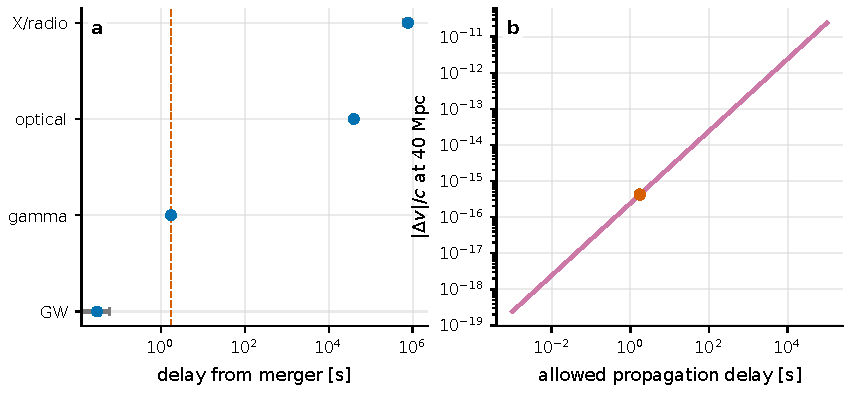
\includegraphics[width=0.92\linewidth]{figures/generated/chapter_13/ch13_multimessenger_delay.pdf}
\caption{Two readings of a multi-messenger delay. The left panel compares the arrival times of the channels after merger: gravitational waves and \(\gamma\)-rays on the second scale, the optical counterpart limited by localization and the day-night cycle and often on the hour scale, and X-rays/radio emerging on day-to-month scales. The right panel converts the propagation delay into the order of magnitude of \(|\Delta v|/c\) at \(40\,\mathrm{Mpc}\), the more uncertain the intra-source emission delay, the more conservative the propagation constraint one can give.}
\label{fig:e20-mm-delay}
\end{figure}

Where does the light of a kilonova come from? From the thermalization of the \(r\)-process (\(r\)-process) radioactive decay in the neutron-rich ejecta. A commonly used scaling is
\begin{equation}
  \dot q(t)\simeq
  2\times10^{10}
  \left(\frac{t}{1\,{\rm d}}\right)^{-1.3}
  {\rm erg\,s^{-1}\,g^{-1}},
  \label{eq:e20-rprocess-heating}
\end{equation}
\begin{formulaexplain}
\(\dot q(t)\) is the heating rate per unit mass of the \(r\)-process material, decaying with time approximately as \(t^{-1.3}\). The power source of a kilonova is not residual heat, not recombination, but this line of radioactive decay.
\end{formulaexplain}
\(\dot q\) is in units of \(\mathrm{erg\,s^{-1}\,g^{-1}}\). What actually enters the luminosity is \(\epsilon_{\rm th}M_{\rm ej}\dot q\), where the thermalization efficiency \(\epsilon_{\rm th}<1\) and \(M_{\rm ej}\) is the ejecta mass. When the light curve peaks is set by the \textbf{diffusion timescale}: the photons must diffuse out from the interior of the ejecta, and the thicker, slower, and more opaque the ejecta, the later they emerge:
\begin{equation}
  t_{\rm pk}\simeq
  \left(\frac{\kappa M_{\rm ej}}{4\pi v_{\rm ej}c}\right)^{1/2}
  =
  0.6\,{\rm d}
  \left(\frac{\kappa}{0.5\,{\rm cm^2\,g^{-1}}}\right)^{1/2}
  \left(\frac{M_{\rm ej}}{0.01M_\odot}\right)^{1/2}
  \left(\frac{v_{\rm ej}}{0.3c}\right)^{-1/2}.
  \label{eq:e20-kilonova-diffusion}
\end{equation}
\begin{formulaexplain}
\(t_{\rm pk}\) is the kilonova peak time, \(\kappa\) is the opacity, \(M_{\rm ej}\) is the ejecta mass, and \(v_{\rm ej}\) is the velocity. The larger the opacity, the larger the mass, and the lower the velocity, the later the peak and the redder the color.
\end{formulaexplain}
Let us verify the \(0.6\,\mathrm{d}\) coefficient: \(\kappa=0.5\,\mathrm{cm^2\,g^{-1}}\), \(M_{\rm ej}=0.01M_\odot=1.99\times10^{31}\,\mathrm{g}\), \(v_{\rm ej}=0.3c=9\times10^9\,\mathrm{cm\,s^{-1}}\), \(c=3\times10^{10}\,\mathrm{cm\,s^{-1}}\). The numerator \(\kappa M_{\rm ej}=9.95\times10^{30}\), the denominator \(4\pi v_{\rm ej}c=4\pi\times9\times10^9\times3\times10^{10}=3.39\times10^{21}\), the ratio \(2.93\times10^{9}\,\mathrm{s^2}\), and taking the square root gives \(5.4\times10^4\,\mathrm{s}\approx0.63\,\mathrm{d}\). The orders of magnitude are then clear: lanthanide-poor ejecta have \(\kappa\sim0.3\text{--}1\,\mathrm{cm^2\,g^{-1}}\), peaking around one day and blueward; lanthanide-rich ejecta have \(\kappa\sim5\text{--}30\,\mathrm{cm^2\,g^{-1}}\), pushing the peak to several days or even ten days and turning toward the near-infrared.

The early spectrum can be approximated by a blackbody, translating the color evolution in one step into radius and temperature:
\begin{equation}
  L_{\rm bol}=4\pi R_{\rm BB}^2\sigma_{\rm SB}T_{\rm BB}^4 .
  \label{eq:e20-kilonova-blackbody}
\end{equation}
\begin{formulaexplain}
\(L_{\rm bol}\) is the total radiative luminosity, \(R_{\rm BB},T_{\rm BB}\) are the blackbody radius and temperature, and \(\sigma_{\rm SB}\) is the Stefan--Boltzmann constant. Given the SED, fitting out \(R_{\rm BB},T_{\rm BB}\) translates ``color changing with time'' into ``the emitting surface is expanding and cooling.''
\end{formulaexplain}
GW170817 at about \(0.6\,\mathrm{d}\) can be described by \(T_{\rm BB}\simeq8300\,\mathrm{K}\), \(R_{\rm BB}\simeq4.5\times10^{14}\,\mathrm{cm}\), \(L_{\rm bol}\simeq5\times10^{41}\,\mathrm{erg\,s^{-1}}\), corresponding to \(v\simeq0.3c\). Subsequently the SED rapidly departed from a single blackbody: the ultraviolet/blue faded while the near-infrared relatively strengthened. This forces at least a two-component model: a blue component with \(M_{\rm ej}\sim0.01M_\odot\), \(v\sim0.27\text{--}0.3c\), and a red component with \(M_{\rm ej}\sim0.04M_\odot\), \(v\sim0.1c\); a three-component model further singles out an intermediate-opacity ``purple component'' \citep{2017Natur.551...75S,2017ApJ...848L..17C,2017ApJ...848L..27T,2017Sci...358.1565E}. A single component cannot explain ``early blue, late red'', which is itself the data telling us that the ejecta has structure.

\begin{figure}[tbp]
\centering
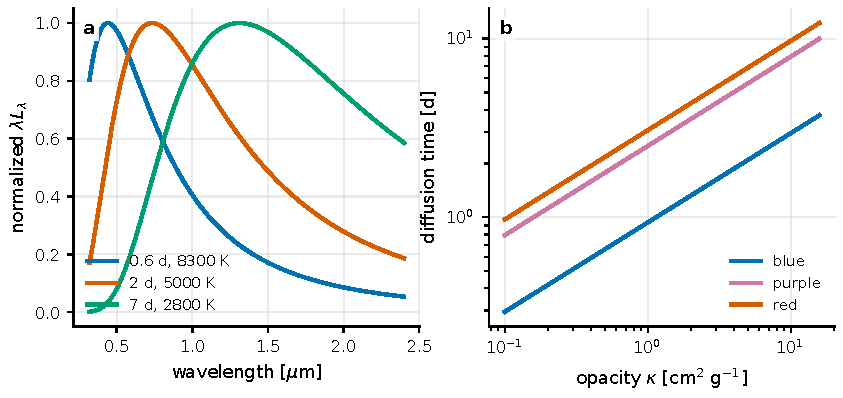
\includegraphics[width=0.92\linewidth]{figures/generated/chapter_13/ch13_kilonova_color_evolution.pdf}
\caption{The blue-to-red evolution of a kilonova. The left panel uses three blackbody SEDs to show the peak wavelength shifting to the infrared as the temperature drops (Wien shift); the right panel uses the diffusion-timescale Equation~\eqref{eq:e20-kilonova-diffusion} to show that the larger the opacity, the larger the mass, and the lower the velocity, the later the peak. GW170817's blue component is fast and low-opacity while its red component is slow and high-opacity, so a single ejecta component cannot simultaneously explain the early blue light and the late near-infrared.}
\label{fig:e20-kilonova}
\end{figure}

Gravitational waves also throw in a bonus treasure, the \textbf{standard siren}: the amplitude of the merger waveform directly gives the luminosity distance, without needing the distance ladder. At low redshift it can be roughly written as
\begin{equation}
  H_0\simeq \frac{cz_{\rm host}}{D_L},
  \label{eq:e20-standard-siren}
\end{equation}
\begin{formulaexplain}
\(H_0\) is the Hubble constant, \(z_{\rm host}\) is the host-galaxy redshift, and \(D_L\) is the luminosity distance given by the gravitational waves. The redshift (recession velocity) divided by the distance is the expansion rate, only here the distance comes from gravitational waves, not from candles.
\end{formulaexplain}
\(z_{\rm host}\) is dimensionless, \(D_L\) is in cm or Mpc, and \(H_0\) is in \(\mathrm{km\,s^{-1}\,Mpc^{-1}}\). The main degeneracy of GW170817 comes from inclination and distance: a binary pointing straight at us is both brighter and harder to constrain in inclination. The electromagnetic counterpart rendered great service here: it gave the host, the redshift, the jet viewing angle, and the ejecta geometry, breaking part of the degeneracy for the gravitational waves. This is the essence of multi-messenger astronomy: a single physical event is projected by gravitational waves, \(\gamma\)-rays, and the optical each onto one facet, and then a joint likelihood stitches them back into a three-dimensional truth.

\section{Gamma-ray burst afterglows: writing the jet geometry into the light-curve slopes}
\label{sec:e20-grb}

The prompt emission of a gamma-ray burst gives the high-energy trigger, but the \textbf{afterglow} is the external-shock physics that can be slowly tracked. After a relativistic thin shell plows into the external medium, the relation between the observed time \(t\) and the shock radius \(R\) and Lorentz factor \(\Gamma\) is approximately
\begin{equation}
  t\simeq \frac{(1+z)R}{4\Gamma^2c}.
  \label{eq:e20-grb-arrival-time}
\end{equation}
\begin{formulaexplain}
\(t\) is the observed arrival time, \(R\) is the shock radius, \(\Gamma\) is the Lorentz factor, and \(z\) is the redshift. The factor \(1/\Gamma^2\) is the combined result of relativistic beaming and the light travel time effect: the source moves almost as fast as the light it emits, compressing a very large \(R\) into an extremely short observed time.
\end{formulaexplain}
The astonishing thing about this formula is that \(\Gamma^2\): a typical early afterglow has \(\Gamma\sim10\text{--}300\), \(R\sim10^{16}\text{--}10^{18}\,\mathrm{cm}\), yet the optical signal can enter the telescope's field of view within tens of seconds to a few minutes after the trigger, an astronomical-scale radius compressed into an observation so fast that only a robotic telescope can chase it \citep{1997ApJ...476..232M,1998ApJ...497L..17S,1998Natur.395..670G,1999PhR...314..575P,2004RvMP...76.1143P,2006ARA&A..44..507W}.

The afterglow light comes from synchrotron radiation by shock-accelerated electrons. Let the electron energy spectrum be a power law:
\begin{equation}
  N(\gamma_e)\,d\gamma_e \propto \gamma_e^{-p}\,d\gamma_e,
  \qquad \gamma_e>\gamma_m,
  \label{eq:e20-electron-powerlaw}
\end{equation}
\begin{formulaexplain}
\(N(\gamma_e)\) is the distribution of the electron Lorentz factor, \(p\) is the energy-spectrum index (typically \(2\text{--}2.5\)), and \(\gamma_m\) is the low-energy cutoff. The slope of the synchrotron afterglow spectrum is ultimately governed by this single number \(p\).
\end{formulaexplain}
Observationally, one usually first compresses the light curve and color into two slopes: the temporal decay index \(\alpha\) and the spectral index \(\beta\):
\begin{equation}
  F_\nu(t)\propto t^{-\alpha}\nu^{-\beta}.
  \label{eq:e20-afterglow-powerlaw}
\end{equation}
\begin{formulaexplain}
\(F_\nu(t)\) is the afterglow flux density, \(\alpha\) governs ``how it dims with time,'' and \(\beta\) governs ``how the spectrum tilts with frequency.'' The two slopes are the afterglow's most compact fingerprint.
\end{formulaexplain}
In a uniform medium, adiabatic, slow-cooling case with the observing frequency in the interval \(\nu_m<\nu<\nu_c\), these two slopes are not independent but are locked together by the same \(p\):
\begin{equation}
  \beta=\frac{p-1}{2},
  \qquad
  \alpha=\frac{3(p-1)}{4}.
  \label{eq:e20-closure-relation}
\end{equation}
\begin{formulaexplain}
This is a \textbf{closure relation}: it binds the observed \(\alpha,\beta\) to the electron index \(p\). If the data clearly deviate from it, then at least one of the assumptions ``simple medium / weak energy injection / non-evolving microphysics'' has collapsed.
\end{formulaexplain}
Dividing the two immediately reveals the structure: \(\alpha/\beta=3/2\), a fixed value independent of \(p\), a hard prediction of this interval. Substituting \(p=2.2\) gives \(\beta\simeq0.6\), \(\alpha\simeq0.9\); if the observing frequency moves to \(\nu>\nu_c\) (the fast-cooling segment), it becomes \(\alpha=(3p-2)/4\). Observationally, an afterglow one day after the burst is often at magnitude \(19\text{--}20\), with polarization reaching a few percent to about \(10\%\), directly related to synchrotron radiation and jet geometry \citep{2004RvMP...76.1143P,2006ARA&A..44..507W}.

\begin{figure}[tbp]
\centering
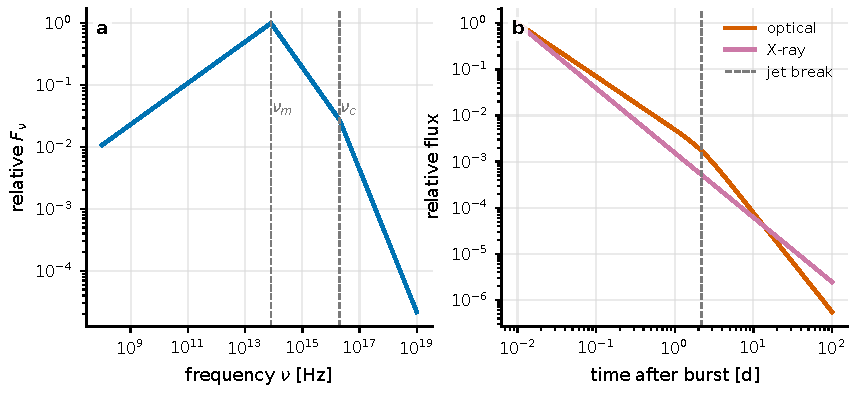
\includegraphics[width=0.92\linewidth]{figures/generated/chapter_13/ch13_afterglow_synchrotron_breaks.pdf}
\caption{The synchrotron reading of a gamma-ray burst afterglow. The left panel shows the characteristic frequencies \(\nu_m\) (minimum electron) and \(\nu_c\) (cooling) slicing the spectrum into intervals of different slope; the right panel shows the light curve steepening across the jet break. If the optical and X-ray are not in the same spectral segment, their \(\alpha,\beta\) need not be the same. One must first judge the position of the observing frequency relative to \(\nu_m,\nu_c\) before applying the closure relation.}
\label{fig:e20-afterglow}
\end{figure}

A jet is not isotropic. When \(\Gamma\) decays to about \(1/\theta_j\), the observer for the first time ``sees the edge of the jet,'' and the light curve exhibits an \textbf{achromatic jet break}. A commonly used estimate is
\begin{equation}
  \theta_j\simeq
  0.10
  \left(\frac{t_j}{1\,{\rm d}}\right)^{3/8}
  \left(\frac{1+z}{2}\right)^{-3/8}
  \left(\frac{E_{\rm iso,52}}{n_0}\right)^{-1/8},
  \label{eq:e20-jet-opening-angle}
\end{equation}
\begin{formulaexplain}
\(\theta_j\) is the jet half-opening angle (rad), \(t_j\) is the jet break time, \(E_{\rm iso,52}\) is the isotropic energy in units of \(10^{52}\,\mathrm{erg}\), and \(n_0\) is the external number density (\(\mathrm{cm^{-3}}\)). The later the break, the wider the jet typically is.
\end{formulaexplain}
Notice those \textbf{very weak} exponents: \(3/8\) and \(1/8\). They are good news for error propagation: even if \(E_{\rm iso}\) or \(n\) each has an order-of-magnitude uncertainty, a factor of \(10\) change in \((E_{\rm iso}/n)\), passed through the \(1/8\) power, changes \(\theta_j\) by only about \(10^{1/8}\approx1.33\) times, i.e.\ thirty percent. The real risk lies not in these parameters but in \textbf{misclassification}: a color-change break, energy injection, a density jump, or even a superimposed supernova bump can all be mistaken for a jet break \citep{2003Natur.423..847H,2004ApJ...611.1005G}. GRB\,980425/SN\,1998bw and GRB\,030329/SN\,2003dh linked long bursts with broad-lined Type Ic supernovae, while the link between short bursts and binary neutron star mergers became multi-messenger ironclad proof after GW170817. Gamma-ray bursts force a telescope system to simultaneously handle a second-scale high-energy trigger, a minute-scale optical flash, an hour-to-day afterglow, and a week-to-month radio calorimetry, and the event table must, besides the flux, keep the time reference and band matching for each stage.

\section{Tidal disruption events: reading the black hole mass from the fallback rate}
\label{sec:e20-tde}

When a star comes too close to a supermassive black hole, it is torn apart, a \textbf{tidal disruption event} (TDE). The tearing occurs inside the tidal radius:
\begin{equation}
  r_t\simeq R_\ast\left(\frac{M_\bullet}{M_\ast}\right)^{1/3},
  \label{eq:e20-tidal-radius}
\end{equation}
\begin{formulaexplain}
\(r_t\) is the tidal radius, \(M_\bullet\) is the black hole mass, and \(M_\ast,R_\ast\) are the stellar mass and radius. Once the star enters within \(r_t\), the gravitational difference of the black hole across its two ends exceeds its own self-gravity, stretching it into a noodle.
\end{formulaexplain}
\(r_t,R_\ast\) are in cm, and \(M_\bullet,M_\ast\) are in g. Whether a bright flare is produced also requires comparison with one more scale, the Schwarzschild radius:
\begin{equation}
  r_s=\frac{2GM_\bullet}{c^2}.
  \label{eq:e20-schwarzschild-radius-tde}
\end{equation}
\begin{formulaexplain}
\(r_s\) is the black hole's Schwarzschild radius. Compare \(r_t\) with \(r_s\): if \(r_t\lesssim r_s\), the star is swallowed whole before it can be torn apart, and no bright flare is seen.
\end{formulaexplain}
Note that \(r_t\propto M_\bullet^{1/3}\) while \(r_s\propto M_\bullet\); the heavier the black hole, the faster \(r_s\) catches up. So main-sequence-star TDEs are most common for \(M_\bullet\sim10^5\text{--}10^7M_\odot\), and around \(10^8M_\odot\), \(r_s\) approaches or even exceeds \(r_t\), and the selection effect grows stronger \citep{1988Natur.333..523R,2021ARA&A..59...21G}.

After being torn apart, half the debris is bound and half escapes. The bound debris that returns to pericenter earliest gives the \textbf{fallback timescale}:
\begin{equation}
  t_{\rm min}\simeq
  41\,{\rm d}
  \left(\frac{M_\bullet}{10^6M_\odot}\right)^{1/2}
  \left(\frac{M_\ast}{M_\odot}\right)^{-1}
  \left(\frac{R_\ast}{R_\odot}\right)^{3/2}.
  \label{eq:e20-tde-fallback-time}
\end{equation}
\begin{formulaexplain}
\(t_{\rm min}\) is the time for the most-bound debris to orbit back to pericenter, given by the Keplerian period of the most-bound orbit, hence growing as \(M_\bullet^{1/2}\). It is the yardstick of the TDE rise timescale.
\end{formulaexplain}
The heavier the black hole, the longer \(t_{\rm min}\) (\(\propto M_\bullet^{1/2}\)), so the rise time itself hides the black hole mass. The fallback rate then transitions into the classic \(t^{-5/3}\) decay:
\begin{equation}
  \dot M_{\rm fb}\simeq
  \frac{M_\ast}{3t_{\rm min}}
  \left(\frac{t}{t_{\rm min}}\right)^{-5/3}.
  \label{eq:e20-tde-fallback-rate}
\end{equation}
\begin{formulaexplain}
\(\dot M_{\rm fb}\) is the debris fallback rate. The ideal \(t^{-5/3}\) decay comes from the uniform distribution of debris energy and is the classic fingerprint of a TDE; but the observed luminosity is also smoothed by circularization (the process by which debris orbits collide, dissipate, and wind into an accretion disk) and reprocessing, and need not follow it strictly.
\end{formulaexplain}
\(\dot M_{\rm fb}\) is commonly in \(M_\odot\,\mathrm{yr^{-1}}\). How fierce is this fallback? Compare it with the Eddington accretion rate:
\begin{equation}
  \dot M_{\rm Edd}
  =
  \frac{L_{\rm Edd}}{\eta c^2}
  \simeq
  0.022
  \left(\frac{M_\bullet}{10^6M_\odot}\right)
  \left(\frac{\eta}{0.1}\right)^{-1}
  M_\odot\,{\rm yr^{-1}} ,
  \label{eq:e20-eddington-rate}
\end{equation}
\begin{formulaexplain}
\(\dot M_{\rm Edd}\) is the Eddington accretion rate, and \(\eta\) is the radiative efficiency. Comparing \(\dot M_{\rm fb}\) with it tells you whether the fallback has surged into a super-Eddington phase.
\end{formulaexplain}
Let us verify the \(0.022\): \(L_{\rm Edd}=1.26\times10^{38}(M_\bullet/M_\odot)\,\mathrm{erg\,s^{-1}}=1.26\times10^{44}\,\mathrm{erg\,s^{-1}}\) (for \(10^6M_\odot\)), \(\eta c^2=0.1\times(3\times10^{10})^2=9\times10^{19}\), so \(\dot M_{\rm Edd}=1.4\times10^{24}\,\mathrm{g\,s^{-1}}\); converting to \(M_\odot\,\mathrm{yr^{-1}}\) (multiply by \(3.156\times10^7\,\mathrm{s\,yr^{-1}}\), divide by \(1.989\times10^{33}\,\mathrm{g}\)) gives \(0.022\). For a \(10^6M_\odot\) black hole, the peak fallback rate of a solar-type star can significantly exceed Eddington, but the \textbf{optical} luminosity need not exceed it likewise, because circularization, stellar winds, obscuration, and reprocessing move the inner-disk energy into the UV/optical and redistribute it.

\begin{figure}[tbp]
\centering
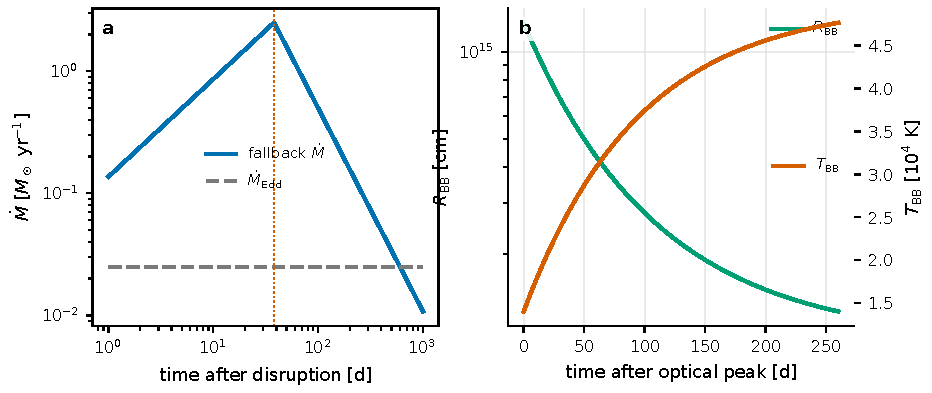
\includegraphics[width=0.92\linewidth]{figures/generated/chapter_13/ch13_tde_fallback_reprocessing.pdf}
\caption{TDE fallback and reprocessing. The left panel shows the \(t^{-5/3}\) fallback entering the decay segment on the scale of tens of days, remaining for a long time above the Eddington accretion rate of a \(10^6M_\odot\) black hole; the right panel gives a typical evolution of the optical/UV blackbody photosphere: the radius contracts from order \(10^{15}\,\mathrm{cm}\) to \(10^{14}\,\mathrm{cm}\), and the temperature rises from order \(10^4\,\mathrm{K}\) to several \(10^4\,\mathrm{K}\).}
\label{fig:e20-tde}
\end{figure}

The blackbody radius of an optical TDE is typically \(10^{14}\text{--}10^{15}\,\mathrm{cm}\), much larger than a few times the \(r_s\) of a \(10^6M_\odot\) black hole; the temperature is often a few \(\times10^4\,\mathrm{K}\), and the evolution is slower than an ordinary supernova. AT2018zr was the first TDE in the early ZTF sample to capture the full rise, with the earliest detection about \(50\,\mathrm{d}\) before peak; its blackbody temperature was about \(1.4\times10^4\,\mathrm{K}\) early on and rose to \(>5\times10^4\,\mathrm{K}\) later, the radius fell from \(10^{15.1}\,\mathrm{cm}\) to \(<10^{14}\,\mathrm{cm}\), and the X-ray luminosity was several orders of magnitude below the contemporaneous optical/UV blackbody, indicating that obscuration or reprocessing cannot be neglected \citep{2019ApJ...872..198V,2021ARA&A..59...21G}. Jetted TDEs (such as Swift\,J1644+57) push the event table toward high energies and rapid variability: the X-rays flicker violently, and the radio tracks the interaction of the outflow with the medium \citep{2011Sci...333..203B}. As for the possible association of TDEs with high-energy neutrinos, that is yet another class of multi-messenger problem requiring a triple coincidence in time, direction, and energy to judge \citep{2021NatAs...5..510S}. Even in such a ``slow'' transient, the event table must still retain complete time information: judging whether a high-energy event belongs to a given optical flare relies on whether the celestial position, time delay, energy, direction error, and source evolution are mutually consistent.

\section{Target-of-opportunity observation: computing ``fast'' and ``error'' together}
\label{sec:e20-tooo}

The success or failure of transient observation is often decided by response speed. But ``fast'' must be quantified, otherwise it is only a slogan. A practical condition is that the total delay from trigger to the first effective exposure must be shorter than the evolution timescale of the source you wish to sample:
\begin{equation}
  t_{\rm alert}+t_{\rm slew}+t_{\rm acq}+t_{\rm exp}
  < f_{\rm samp}\,t_{\rm evol},
  \label{eq:e20-response-budget}
\end{equation}
\begin{formulaexplain}
The left side is the response budget: alert issuance \(t_{\rm alert}\) + telescope slewing \(t_{\rm slew}\) + target confirmation and guiding \(t_{\rm acq}\) + the first effective exposure \(t_{\rm exp}\); the right side is the source evolution timescale \(t_{\rm evol}\) you wish to sample, times a sampling factor \(f_{\rm samp}\). Target-of-opportunity observation is about satisfying this inequality.
\end{formulaexplain}
If you want to \textbf{resolve} the rise rather than just catch a single point, then \(f_{\rm samp}\sim0.1\) is reasonable (the sampling must be ten times faster than the evolution). Substituting the various source types of this chapter: the \(t_{\rm evol}\) of a GRB optical flash can be less than \(10^3\,\mathrm{s}\), the blue-light phase of a GW counterpart is about one day, the early radio/spectral structure of a nova changes within days to weeks, and the rise timescale of a TDE is often tens of days. The same formula turns ``how fast, exactly'' from an emotion into a checkable number.

Having secured the target, one must still compute whether the exposure is deep enough. The signal-to-noise ratio of ordinary imaging is
\begin{equation}
  {\rm SNR}=
  \frac{N_s}
  {\left(N_s+N_b+n_{\rm pix}\sigma_{\rm read}^2\right)^{1/2}},
  \label{eq:e20-imaging-snr}
\end{equation}
\begin{formulaexplain}
\({\rm SNR}\) is the imaging signal-to-noise ratio, \(N_s\) is the source count, \(N_b\) is the background count, and \(n_{\rm pix}\sigma_{\rm read}^2\) is the read noise summed over the pixels within the aperture. Those three terms in the denominator are precisely the sum of the three kinds of error: ``source's own fluctuation + background fluctuation + electronic noise.''
\end{formulaexplain}
\(N_s,N_b\) are counts (dimensionless), \(n_{\rm pix}\) is the number of pixels within the aperture, and \(\sigma_{\rm read}\) is the read noise per pixel (in electrons). When the source is bright (\(N_s\gg N_b,\,n_{\rm pix}\sigma_{\rm read}^2\)), the denominator tends to \(\sqrt{N_s}\), recovering the shot-noise limit \({\rm SNR}\to\sqrt{N_s}\) of Chapter~\ref{chap:e03}; when the source is faint, the background and read noise take over, which is precisely why deep-field transients are hard to do.

Finally, do not forget that \textbf{host association} is also a statistical judgment with errors, not ``it looks close so it must be a match.'' If the transient localization error radius is \(r\) and the surface density of background galaxies down to depth \(m\) is \(\Sigma(<m)\), then the \textbf{chance coincidence probability} of randomly hitting a background galaxy is
\begin{equation}
  P_{\rm cc}=1-\exp[-\pi r^2\Sigma(<m)].
  \label{eq:e20-chance-coincidence}
\end{equation}
\begin{formulaexplain}
\(P_{\rm cc}\) is the chance host-coincidence probability, \(r\) is the localization error radius, and \(\Sigma(<m)\) is the surface density of background galaxies. It is in fact a Poisson result: the probability that ``there is at least one background galaxy within the error circle'' is \(1-e^{-\langle N\rangle}\), with the expected number \(\langle N\rangle=\pi r^2\Sigma\).
\end{formulaexplain}
In this expression \(r\) is in rad or arcsec, \(\Sigma(<m)\) is the number of galaxies per unit solid angle (e.g.\ \(\mathrm{arcsec^{-2}}\)), and the product \(\pi r^2\Sigma\) is dimensionless. The worse the localization and the denser the galaxies, the larger \(P_{\rm cc}\) and the less trustworthy the host association. GW170817 relied on the addition of the Virgo detector to shrink the sky region from over a hundred to a few tens of square degrees, allowing the optical survey to lock down the host on the same night; TDEs, conversely, require sub-arcsecond astrometry to prove that the flare truly sits at the galactic nucleus. The same \(P_{\rm cc}\) governs everything from gravitational-wave localization to nuclear-transient confirmation \citep{2017PhRvL.119p1101A,2017ApJ...848L..12A,2019ApJ...872..198V}.

Listing the timescales, observables, and main risks of the six source classes of this chapter side by side, for easy comparison:
\begin{longtable}{@{}p{0.14\linewidth}p{0.18\linewidth}p{0.28\linewidth}p{0.28\linewidth}@{}}
\toprule
Source class & Key timescale & Typical observables & Main risk \\
\midrule
Classical nova & Days to months & Line velocity, radio angular scale, \(\gamma\)-ray window & Multiple velocity components bias the expansion parallax. \\
Type Ia supernova & Days to weeks & Light-curve width, color, Si\,II velocity, polarization, microarcsecond angular scale & Luminosity calibration and angular scale come from different physical layers. \\
Core-collapse & Minutes to days & UV/soft X-ray outburst, early spectrum, polarization & Triggering too late misses the progenitor-radius information. \\
Kilonova & Hours to ten days & GW distance, \(\gamma\)-ray delay, color and near-infrared evolution & Opacity, viewing angle, and ejecta geometry are mutually degenerate. \\
Gamma-ray burst & Seconds to months & \(\alpha,\beta\), jet break, polarization, radio calorimetry & A color-change break or energy injection misjudges the jet geometry. \\
Tidal disruption & Weeks to years & Rise timescale, nuclear position, \(T_{\rm BB}\), \(R_{\rm BB}\), X-ray/optical ratio & AGN-variable contamination and non-unique reprocessing geometry. \\
\bottomrule
\end{longtable}

\section*{Chapter Summary}
\addcontentsline{toc}{section}{Chapter Summary}

\begin{itemize}
  \item \textbf{The information of a transient is in time.} The light curve is a binned product that smears away the onset time and fine structure; the unbinned inhomogeneous Poisson likelihood Equation~\eqref{eq:e20-poisson-likelihood} eats the event times \(t_j\) directly, which is precisely why Chapter~\ref{chap:e13} insists on keeping the time/frequency/polarization label of every photon.
  \item \textbf{Triggering is inference, not an alarm.} Use the odds ratio Equation~\eqref{eq:e20-trigger-odds} to put ``prior rarity'' and ``data likelihood'' into the judgment together; false triggers are controlled by the Poisson-tail probability Equation~\eqref{eq:e20-false-alarm}, but the true number of false alarms must be multiplied by the trials factor over time windows, pixels, energy channels, and templates.
  \item \textbf{Transient sources are mostly thermal chaotic light.} The coherence time of a broadband blackbody photosphere is only a femtosecond (\(\tau_c\simeq1/\Delta\nu\)), and within a millisecond bin the counts degenerate into pure Poisson shot noise; to touch the coherence information one must rely on nanosecond/picosecond intensity interferometry, whose precision is set by the photon-pair number Equation~\eqref{eq:e20-pair-statistics}. Coherent emission such as FRBs and pulsars exposes itself through an extremely high brightness temperature.
  \item \textbf{Geometry links speed, time, and angular scale into a cosmic ruler.} The angular-expansion Equation~\eqref{eq:e20-angular-expansion} plus the spectral-line velocity Equation~\eqref{eq:e20-doppler-line} give the expansion parallax Equation~\eqref{eq:e20-expansion-parallax}, but the velocity and the angular scale must correspond to the same material layer, otherwise the distance is systematically biased.
  \item \textbf{Multi-messenger astronomy is stitched by time.} A delay is meaningful only under a unified time standard (Equation~\eqref{eq:e20-mm-delay}), and must be split into intra-source emission, propagation, and clock parts (Equation~\eqref{eq:e20-delay-budget}); great distance lets a second-scale delay correspond to a speed-difference constraint of \(\sim10^{-16}\) (Equation~\eqref{eq:e20-speed-difference}).
  \item \textbf{``Fast'' must be quantified, and the host must be verified.} The response budget Equation~\eqref{eq:e20-response-budget} turns speed into a checkable inequality; the chance-coincidence probability Equation~\eqref{eq:e20-chance-coincidence} reminds us that host association, like triggering, is a statistical judgment with errors. The error budget of Chapter~\ref{chap:e15} will fold all of these into the feasibility analysis.
\end{itemize}

\medskip
\noindent\textbf{Questions to Ponder}
\begin{itemize}
  \item A GRB trigger uses a window of \(\Delta t=0.05\,\mathrm{s}\) and a background rate \(b=2\,\mathrm{s^{-1}}\). If one night searches \(10^{9}\) independent windows, roughly what trigger threshold \(n\) should be chosen to keep the expected number of false alarms below 1? (Hint: use Equation~\eqref{eq:e20-false-alarm} to first compute the single-window \(P_{\rm FA}\), then multiply by the number of trials.)
  \item If the spectral line of a nova gives the outermost \(v_{\rm exp}=1.5\times10^8\,\mathrm{cm\,s^{-1}}\), while the angular scale actually comes from a more interior continuum photosphere with a velocity only \(0.7\) times as large, will the distance obtained from Equation~\eqref{eq:e20-expansion-parallax} be too large or too small, and by how much?
  \item Why, when doing photometry of a broadband thermal transient, can one safely use \(\sqrt N\) errors, whereas doing intensity interferometry one must return to the photon-pair number Equation~\eqref{eq:e20-pair-statistics}? At which time scale is each of the two ``looking at'' the signal?
\end{itemize}


% ============================================================
\part{Propagation, Cosmology, and New Physics}
\chapter{Propagation Effects: Plasma, Dust, and Gravitational Lensing}
\label{chap:e21}

\begin{chapteropening}
Up to now we have almost always been asking the same kind of question: \textbf{what does the source really look like?}: its angular diameter, its coherence time, its photon statistics. But there is one thing we have quietly been assuming away: that as light sets out from the source and flies all the way to the telescope, the intervening thousands of light-years, the billions of light-years, are ``transparent.'' Of course they are not. Light must pass through tenuous free electrons, turbulent magnetized plasma, nebulae full of drifting dust grains, and even spacetime bent by massive objects. Every layer it crosses silently rewrites its arrival time, frequency, polarization, direction, and even ``how many copies it has.''

This chapter is about making clear ``what happens along the way.'' The through-line is as follows. First we treat propagation as a \textbf{channel with memory}, it does not simply multiply the signal by a constant, but refills every label carried by each photon. Then we take apart four classes of rewriters one by one: the \(\nu^{-2}\) dispersion of cold plasma (we will derive, without skipping a single step, ``why low-frequency photons arrive late''), the scattering and scintillation brought by turbulence, the extinction and reddening of dust, and the gravitational lensing of curved spacetime. Finally we return to the book's home turf: these effects both \textbf{contaminate} the signal (smearing out coherence, scrambling time stamps) and \textbf{encode} it (storing an electron ledger in the dispersion measure, storing cosmology in the time delay). It follows on from the bandwidth and coherence time of Chapter~\ref{chap:e02} and the time synchronization of Chapter~\ref{chap:e13}, and is the last processing step that translates ``source-end physics'' into ``detector events.''
\end{chapteropening}

\section{Treating propagation as a channel with memory}
\label{sec:e21-channel}

Let us set the scene. The easiest idea is to treat the medium as a piece of gray glass: light passes through, a little dimmer, a little redder, everything else unchanged. For average brightness and average color, this ``multiply by a constant'' picture is sometimes sufficient. But what this book cares about is the \textbf{event table} (Chapter~\ref{chap:e13}), each photon candidate carrying the labels of arrival time, frequency, polarization, and direction; and it also cares about \textbf{coherence}, the phase relations of the field between different times and different telescopes. For these quantities, ``gray glass'' is a catastrophic approximation, because what propagation really does is \textbf{rewrite the labels}: the frequency label determines how late it arrives, the polarization label is rotated by the magnetic field, the direction label is scattered apart and copied by the lens, and the arrival-time label is dragged out into echoes by multiple paths.

So a better first step is not to ask ``how bright was the source really,'' but to ask ``through what kind of channel must the source-end field pass to become an event on my detector.'' Writing it as a linear channel is the most direct. In the time domain, the electric field of the \(i\)-th observation channel (a given polarization, a given telescope, a given image, a given frequency channel) is the \textbf{convolutional superposition} of the source-end channel fields:
\begin{equation}
  E_{{\rm out},i}(t)
  =
  \sum_j\int h_{ij}(t-t')\,E_{{\rm src},j}(t')\,{\rm d}t'
  + n_i(t) .
  \label{eq:e21-channel-time}
\end{equation}
\begin{formulaexplain}
\(E_{{\rm out},i}\) is the field of the \(i\)-th observation channel, \(E_{{\rm src},j}\) is the field of the \(j\)-th source-end channel, \(h_{ij}\) is the response function from \(j\) to \(i\), and \(n_i\) is the foreground and detection noise. The integral sign is the key: propagation \textbf{has memory}: the light from one source-end instant is delayed and broadened to contribute to many observed instants.
\end{formulaexplain}
Symbol by symbol: \(i,j\) label polarization, telescope, image, or frequency channel (dimensionless indices); \(h_{ij}(t-t')\) is the impulse response, whose dimension depends on the field normalization, but what is truly useful are its three characteristics: the \textbf{time width} (how much the signal is broadened), the \textbf{peak delay} (how much the signal as a whole arrives late), and the \textbf{relative phase} between different channels; \(n_i(t)\) is the sum of foreground thermal radiation, airglow background, and detection-chain noise. If the medium only absorbs and does not scatter, \(h_{ij}\) is approximately a diagonal, amplitude-suppressed delta function; if there is Faraday rotation, it ``transfers funds'' between two linear polarization channels; if there is scattering or lensing, it simultaneously stirs together direction and arrival time. The barycentric correction, clock offsets, atmospheric delay, and instrumental electronic delay are also all part of this \(h_{ij}\): pulsar timing is precisely the most mature paradigm for taking these terms apart one by one down to the nanosecond level \citep{2006MNRAS.372.1549E}.

Translating back into the language of the event table: a photon candidate is a row \((t_q,\nu_q,p_q,\bm{x}_q,w_q)\): arrival time \(t_q\) (in s), frequency \(\nu_q\) (in Hz), polarization channel \(p_q\), spatial label \(\bm{x}_q\) (pixel, baseline, or telescope index), and quality weight \(w_q\). What remains to be done in this section is to write out a concrete form of that abstract \(h_{ij}\) in Equation~\eqref{eq:e21-channel-time} for each of the four classes of medium, seeing exactly how it modifies these five labels: dispersion modifies \(t_q(\nu_q)\), Faraday rotation modifies \(p_q(\lambda_q^2)\), scattering spreads the \(t_q\) of a narrow pulse into a long tail, dust modifies the probability that a given \(\lambda_q\) is received, and lensing copies one source event into several sets of \((\bm{x}_q,t_q)\).

Before beginning, let us spread the \textbf{map of orders of magnitude} out on the table, so that later, whenever we compute a number, we know where we stand. The dispersion measure (which we will define shortly) of the Galaxy toward high Galactic latitude is often \(30\text{--}100\,{\rm pc\,cm^{-3}}\), while fast radio bursts (FRBs) can reach \(10^{3}\text{--}10^{4}\,{\rm pc\,cm^{-3}}\). The rotation measure of the ordinary interstellar medium is mostly \(1\text{--}10^{2}\,{\rm rad\,m^{-2}}\), reaching \(10^{4}\text{--}10^{5}\,{\rm rad\,m^{-2}}\) in strongly magnetized dense environments. Scattering broadening ranges from microseconds to seconds, growing extremely fast at the low-frequency end. Optical extinction is often less than \(0.1\) magnitude at high Galactic latitude, and can reach several magnitudes in the Galactic disk and molecular clouds. The time delay of gravitational lensing spans the largest range: stellar-mass lenses give microseconds to milliseconds, and galaxy strong lensing is often days to years. Keep this map in mind, and every formula in this chapter can be pinned to a real number.

\section{Cold plasma dispersion: why low-frequency photons arrive late}
\label{sec:e21-dispersion}

Let us pick out the cleanest of the rewriters: cold plasma, that is, the tenuous free electrons pervading interstellar and intergalactic space. It has a very mild and very useful property: it does not randomize the pulse, but merely makes \textbf{low-frequency photons arrive slightly late}. And ``how late'' is precisely proportional to the total number of electrons encountered along the way. That is to say, dispersion is both a ``contaminant'' (it smears an instantaneous burst into a swept slanted line in frequency) and an ``encoder'' (the slope of that line is the electron ledger along the line of sight). We will derive this \(\nu^{-2}\) law without skipping a single step.

\paragraph{From refractive index to group velocity}
\label{sec:e21-groupvel}

The response of free electrons to an electromagnetic wave gives the refractive index of cold plasma. When the wave frequency is much higher than the plasma frequency (we will verify shortly that this condition holds for radio observation),
\begin{equation}
  n(\omega)\simeq 1-\frac{\omega_p^2}{2\omega^2},
  \qquad
  \omega_p^2=\frac{4\pi n_e e^2}{m_e}.
  \label{eq:e21-plasma-index}
\end{equation}
\begin{formulaexplain}
\(n(\omega)\) is the refractive index (dimensionless), \(\omega\) is the angular frequency, \(\omega_p\) is the plasma frequency, \(n_e\) is the free-electron number density, and \(e,m_e\) are the electron charge and mass (CGS units). The more electrons, the larger \(\omega_p\), and the more markedly a low-frequency wave deviates from vacuum propagation.
\end{formulaexplain}
Symbol by symbol: \(n_e\) is in \({\rm cm^{-3}}\), commonly \(10^{-2}\text{--}10^{-1}\,{\rm cm^{-3}}\) in the Galactic warm ionized medium and many orders of magnitude higher in HII regions and FRB host environments; \(\omega_p=\sqrt{4\pi n_e e^2/m_e}\) is the plasma's own natural oscillation frequency (in \({\rm rad\,s^{-1}}\)). Let us plug in a number to get a feel: taking \(n_e=0.03\,{\rm cm^{-3}}\), with the CGS values \(e=4.8\times10^{-10}\,{\rm esu}\), \(m_e=9.1\times10^{-28}\,{\rm g}\), gives \(\omega_p\approx 9.8\times10^{3}\,{\rm rad\,s^{-1}}\), corresponding to a frequency \(\nu_p=\omega_p/2\pi\approx1.5\,{\rm kHz}\). And radio observation is at \(\nu\sim10^{8}\text{--}10^{9}\,{\rm Hz}\), so \(\omega\gg\omega_p\) holds extremely amply, and keeping only the first order in \(\omega_p^2/\omega^2\) in Equation~\eqref{eq:e21-plasma-index} is entirely sufficient.

The crucial physics is that information (the pulse envelope) does not propagate at the phase velocity but at the \textbf{group velocity} \(v_g={\rm d}\omega/{\rm d}k\), as was stressed back in Chapter~\ref{chap:e02} when discussing wave packets. To compute \(v_g\), first write the dispersion relation \(k=n\omega/c\):
\[
  k=\frac{n\omega}{c}
   =\frac{\omega}{c}\left(1-\frac{\omega_p^2}{2\omega^2}\right)
   =\frac{\omega}{c}-\frac{\omega_p^2}{2c\,\omega}.
\]
Differentiating term by term with respect to \(\omega\) (using \({\rm d}(\omega^{-1})/{\rm d}\omega=-\omega^{-2}\) for the second term):
\[
  \frac{{\rm d}k}{{\rm d}\omega}
  =\frac{1}{c}-\frac{\omega_p^2}{2c}\cdot\left(-\frac{1}{\omega^2}\right)
  =\frac{1}{c}\left(1+\frac{\omega_p^2}{2\omega^2}\right).
\]
The group velocity is its reciprocal, expanded to first order using the geometric series \((1+x)^{-1}\approx1-x\) (because \(x=\omega_p^2/2\omega^2\ll1\)):
\[
  v_g=\frac{{\rm d}\omega}{{\rm d}k}
     =\frac{c}{1+\dfrac{\omega_p^2}{2\omega^2}}
     \approx c\left(1-\frac{\omega_p^2}{2\omega^2}\right).
\]
This step already lets us ``see'' the physics: \(v_g<c\), and \textbf{the lower the frequency (the smaller \(\omega\)), the larger \(\omega_p^2/2\omega^2\), and the slower the group velocity}. Slow means arriving late. The root cause of low-frequency photons arriving late is this one line.

\paragraph{Summing up the delay along the line of sight}
\label{sec:e21-dmderive}

Now let us translate ``slow'' into ``how late.'' A path segment \({\rm d}l\) takes a time \({\rm d}l/v_g\); integrating along the whole line of sight:
\[
  t=\int\frac{{\rm d}l}{v_g}
   =\int\frac{1}{c}\left(1+\frac{\omega_p^2}{2\omega^2}\right){\rm d}l
   =\underbrace{\frac{L}{c}}_{\text{vacuum flight}}
   +\underbrace{\frac{1}{2c\,\omega^2}\int\omega_p^2\,{\rm d}l}_{\text{extra dispersive delay}} .
\]
The first term is the time for light to fly the whole path \(L\) in vacuum, independent of frequency, and observationally only a total zero point that cannot be measured. What can truly be measured is the second term: it is the \textbf{frequency-dependent} lateness. Substituting \(\omega_p^2=4\pi n_e e^2/m_e\), and noting that \(4\pi e^2/m_e\) is a constant that can be pulled outside the integral:
\[
  \Delta t
  =\frac{1}{2c\,\omega^2}\int\frac{4\pi n_e e^2}{m_e}\,{\rm d}l
  =\frac{2\pi e^2}{m_e c\,\omega^2}\int n_e\,{\rm d}l .
\]
Finally, using \(\omega=2\pi\nu\), i.e.\ \(\omega^2=4\pi^2\nu^2\):
\begin{equation}
  \Delta t
  =\frac{e^2}{2\pi m_e c}\,\frac{1}{\nu^2}\int n_e\,{\rm d}l
  \equiv \frac{e^2}{2\pi m_e c}\,\frac{{\rm DM}}{\nu^2},
  \qquad
  {\rm DM}\equiv\int n_e\,{\rm d}l .
  \label{eq:e21-dm-delay}
\end{equation}
\begin{formulaexplain}
\(\Delta t\) is the extra delay relative to vacuum, \(\nu\) is the observing frequency, and DM is the \textbf{dispersion measure}, i.e.\ the column density of free electrons along the line of sight \(\int n_e\,{\rm d}l\). The skeleton of the whole expression is \(\Delta t\propto {\rm DM}/\nu^{2}\): the lateness is proportional to the total number of electrons along the way and inversely proportional to the square of the frequency.
\end{formulaexplain}
This expression makes three things clear at once. First, \(\Delta t\propto\nu^{-2}\): this is the quantitative version of ``low frequency arrives late,'' and we derived it all the way from the group velocity with no skipped steps. Second, the constant out front, \(e^2/(2\pi m_e c)\), is a pure physical constant (in CGS); substituting the astronomer's customary pc for the path element \({\rm d}l\) of DM and GHz for the frequency, the delay difference between two frequency channels is the one every astronomer knows by heart:
\begin{equation}
  \Delta t_{\rm DM}
  =
  4.148808\,{\rm ms}\;
  \frac{{\rm DM}}{{\rm pc\,cm^{-3}}}
  \left[
  \left(\frac{\nu_1}{\rm GHz}\right)^{-2}
  -
  \left(\frac{\nu_2}{\rm GHz}\right)^{-2}
  \right].
  \label{eq:e21-dispersion-delay}
\end{equation}
\begin{formulaexplain}
\(\Delta t_{\rm DM}\) is the arrival-time difference between the two channels at frequencies \(\nu_1\) and \(\nu_2\). The coefficient \(4.148808\,{\rm ms}\) is just the value of the physical constant in Equation~\eqref{eq:e21-dm-delay} after converting to pc, \({\rm cm^{-3}}\), and GHz. The \(\nu_1^{-2}\) term for the low frequency (\(\nu_1<\nu_2\)) is larger, so the low-frequency channel arrives late, and what one sees in the dynamic spectrum is that swept trajectory bending down and to the right.
\end{formulaexplain}
Third, DM is a \textbf{column density, not a local density}: it cares only about how many electrons there are in total along the way, not about how they are distributed. Its unit is \({\rm pc\,cm^{-3}}\) (the length pc multiplied by the number density \({\rm cm^{-3}}\)).

Let us plug in a real number. Take \({\rm DM}=300\,{\rm pc\,cm^{-3}}\) (a typical value for a moderate-distance pulsar), \(\nu_1=0.6\,{\rm GHz}\), \(\nu_2=1.4\,{\rm GHz}\):
\[
  \Delta t_{\rm DM}=4.148808\times300\times\left(0.6^{-2}-1.4^{-2}\right)\,{\rm ms}
  \approx 1244.6\times(2.778-0.510)\,{\rm ms}\approx 2822\,{\rm ms}\approx 2.8\,{\rm s}.
\]
Nearly three seconds! From the same burst, the \(0.6\) GHz signal arrives almost three seconds later than the \(1.4\) GHz. Precisely for this reason, radio-pulse and FRB searches must first perform \textbf{de-dispersion} over a bank of trial dispersion measures (trial DMs), shifting each frequency channel back according to \(\nu^{-2}\) until the pulses in the different channels realign and the signal-to-noise spikes; the DM that maximizes the signal-to-noise is the measured value.

There is also an easily overlooked \textbf{contamination}: even if the overall de-dispersion is done correctly, each frequency channel itself has a finite bandwidth \(\Delta\nu\), and the delay difference between the high- and low-frequency ends within the channel has not been compensated, which smears the pulse wider:
\begin{equation}
  \Delta t_{\rm chan}
  \simeq
  8.3\,\mu{\rm s}\;
  \left(\frac{{\rm DM}}{{\rm pc\,cm^{-3}}}\right)
  \left(\frac{\Delta\nu}{\rm MHz}\right)
  \left(\frac{\nu}{\rm GHz}\right)^{-3}.
  \label{eq:e21-channel-smearing}
\end{equation}
\begin{formulaexplain}
\(\Delta t_{\rm chan}\) is the residual dispersive broadening within a finite-bandwidth channel, \(\Delta\nu\) is the channel bandwidth, and \(\nu\) is the channel center frequency. It is the result of differentiating Equation~\eqref{eq:e21-dispersion-delay} with respect to \(\nu\) and multiplying by \(\Delta\nu\), hence the \(\nu^{-3}\). The meaning: the higher the DM, the wider the channel, and the lower the frequency, the more easily microsecond-scale fine structure is washed flat.
\end{formulaexplain}
It is of one spirit with Chapter~\ref{chap:e02}: to obtain good time resolution, one must pay the price in bandwidth, only here the price is amplified by dispersion. For high-time-resolution astronomy, Equation~\eqref{eq:e21-channel-smearing} directly determines how finely the channels must be sliced.

\begin{figure}[tbp]
\centering
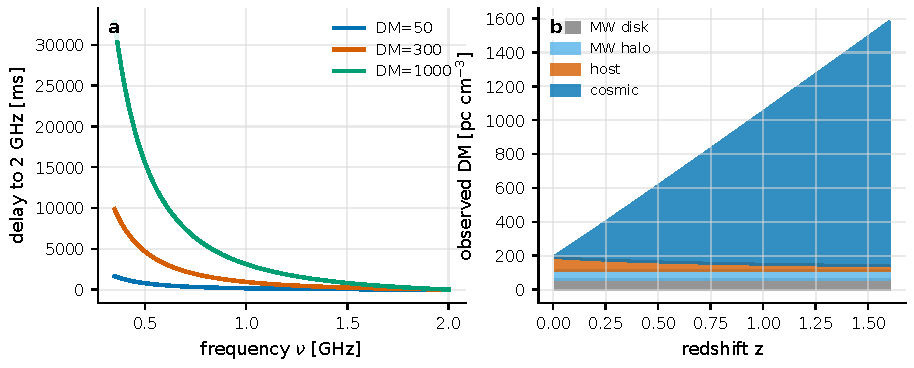
\includegraphics[width=0.94\linewidth]{figures/generated/chapter_14/ch14_dispersion_delay.pdf}
\caption{Cold-plasma dispersion and the FRB dispersion-measure budget. The left panel plots the arrival delay as a function of frequency (reference frequency \(2\,{\rm GHz}\)): the steep \(\nu^{-2}\) curve at the low-frequency end is why Equation~\eqref{eq:e21-dispersion-delay} makes DM so easy to read out from a broadband dynamic spectrum. The right panel breaks the observed dispersion measure of a nearby FRB into four parts: Galactic disk, Galactic halo, host galaxy, and cosmological plasma; the host term enters the observed value with a factor \((1+z)^{-1}\) because of cosmological time dilation.}
\label{fig:e21-dispersion}
\end{figure}

\paragraph{The dispersion measure as an electron ledger: from the Galaxy to cosmology}
\label{sec:e21-dmbudget}

Since DM is an electron ledger, one can conversely use it to measure electrons. But the ledger must sort out who owes what. The Galactic electron density is by no means constant: the NE2001 model stitches together the thick disk, thin disk, spiral arms, local bubble, and clumps, constraining the parameters with pulsar DMs, independent distances, and scattering data; YMW16 updated the thick disk, thin disk, spiral arms, Galactic center, and the treatment of the Magellanic Clouds/intergalactic medium, specifically to convert the \textbf{Galactic part of the DM} of a pulsar or an FRB into a distance or a foreground \citep{2002astro.ph..7156C,2017ApJ...835...29Y}. The Galactic-disk contribution of a high-Galactic-latitude line of sight is often \(30\text{--}100\,{\rm pc\,cm^{-3}}\), with the Galactic halo adding an order of \(50\text{--}100\,{\rm pc\,cm^{-3}}\); near the Galactic disk, an HII region, or a supernova remnant, local structure becomes more important than a smooth model.

For a cosmological FRB, the total observed dispersion measure is a bill spanning billions of light-years:
\begin{equation}
  {\rm DM}_{\rm FRB}
  =
  {\rm DM}_{\rm MW,ISM}
  +{\rm DM}_{\rm MW,halo}
  +{\rm DM}_{\rm cosmic}(z)
  +\frac{{\rm DM}_{\rm host}}{1+z} .
  \label{eq:e21-frb-dm-budget}
\end{equation}
\begin{formulaexplain}
The four terms are the contributions of the Galactic disk, the Galactic halo, the cosmological plasma along the way, and the host galaxy. The host term must be divided by \((1+z)\), because the frequency intervals and time intervals emitted at the host have already been stretched by a factor of the redshift by cosmic expansion en route to us. The same physical delay looks smaller to us.
\end{formulaexplain}
The physical meaning of each term: the first two come from our own Galaxy and can be subtracted using NE2001/YMW16; \({\rm DM}_{\rm cosmic}(z)\) is the baryonic electrons diffuse in the intergalactic medium, growing monotonically with redshift, and is the most valuable term in this expression; \({\rm DM}_{\rm host}\) is the host-galaxy contribution and is the hardest to constrain. Writing the cosmological term as an integral over a homogeneous universe:
\begin{equation}
  {\rm DM}_{\rm cosmic}(z)
  =
  \frac{3cH_0\Omega_b f_{\rm IGM}}{8\pi Gm_p}
  \int_0^z
  \frac{f_e(z')(1+z')}{\sqrt{\Omega_m(1+z')^3+\Omega_\Lambda}}
  \,{\rm d}z' .
  \label{eq:e21-cosmic-dm}
\end{equation}
\begin{formulaexplain}
\(\Omega_b,\Omega_m,\Omega_\Lambda\) are the baryon, matter, and dark-energy density parameters, \(H_0\) is the Hubble constant, \(m_p\) is the proton mass, \(f_{\rm IGM}\) is the fraction of baryons in the diffuse intergalactic medium, and \(f_e\) is the number of free electrons provided per baryon. The coefficient out front gives the mean baryon density, and the integrand describes how the electron number density and path length vary with redshift in an expanding universe.
\end{formulaexplain}
None of the components of this expression is mysterious: the coefficient \(3H_0^2\Omega_b/8\pi G\) is today's mean baryon mass density (the critical density times \(\Omega_b\)), divided by \(m_p\) to become a number density, then times \(f_e f_{\rm IGM}\) to give the electron number density; the \((1+z')\) in the integral is the net factor after the dilution of density by expansion is offset by the compression of the path, and the denominator \(\sqrt{\Omega_m(1+z')^3+\Omega_\Lambda}\) is the \(\Lambda\)CDM expansion rate \(H(z')/H_0\). There is one step here that must not be dropped: the line-of-sight element is not \({\rm d}l\) but rather \({\rm d}l=c\,{\rm d}z'/H(z')\) written in terms of redshift, which alone contributes a factor \(c/H_0\) (with \(H_0\) pulled out of \(H(z')=H_0\sqrt{\cdots}\) and placed in the denominator of the integrand). It is precisely this \(c/H_0\), merging with the \(H_0^2\) in the critical density, that turns the prefactor from the mass-density form ``\(3H_0^2\Omega_b/(8\pi G)\) divided by \(m_p\)'' into the \(3cH_0\Omega_b f_{\rm IGM}/(8\pi Gm_p)\) with \(cH_0\) in the expression, one factor of \(c/H_0\) more than the pure mass density. If the reader works through the algebra, do remember this share of \(c/H_0\) coming from \({\rm d}l=c\,{\rm d}z'/H(z')\), otherwise the prefactor will be off by a factor. Its physical meaning is astonishingly practical: \textbf{the DM--redshift relation of FRBs directly weighs how many baryons there are in the universe}: this was once the ``missing baryon'' problem, and today the relation given by FRB samples can already measure the cosmic baryon content. The true scatter comes from the inhomogeneity of the cosmic web, often written as \(\sigma_{\rm DM}\simeq F z^{-1/2}\), with \(F\sim0.1\text{--}0.4\) corresponding to different feedback and halo-gas distributions \citep{2020Natur.581..391M,2014ApJ...790..101S}. This is the most beautiful example of ``contamination becoming encoding'': dispersion was originally a fog standing in front of the source, and it turns out that this fog itself weighs the baryons of the universe.

\section{Faraday rotation: adding the direction of the magnetic field to dispersion}
\label{sec:e21-faraday}

Dispersion counts only the number of electrons and throws away the information of the magnetic field. If the plasma is \textbf{magnetized}, there is a second imprint: left- and right-handed circular polarizations have different phase velocities in a magnetized plasma, so the plane of vibration of linear polarization is rotated as it propagates, and the rotation angle is precisely proportional to the square of the wavelength:
\begin{equation}
  \psi(\lambda)=\psi_0+{\rm RM}\,\lambda^2 .
  \label{eq:e21-rm-angle}
\end{equation}
\begin{formulaexplain}
\(\psi\) is the observed linear polarization angle, \(\psi_0\) is the source's intrinsic polarization angle, \(\lambda\) is the wavelength, and RM is the \textbf{rotation measure}. The slope of the polarization angle against \(\lambda^2\) is RM. So as long as one measures the polarization angle at several frequencies and plots it as a \(\psi\)--\(\lambda^2\) diagram, the slope gives the cumulative effect of the magnetized plasma.
\end{formulaexplain}
It is a sister to dispersion: dispersion gives the arrival time a slope of \(\nu^{-2}\) (equivalent to \(\lambda^2\)), while Faraday gives the polarization angle a slope of \(\lambda^2\). Both are ``reading a slope.'' The rotation measure itself is the path integral of the electron density and the line-of-sight magnetic-field component:
\begin{equation}
  {\rm RM}
  =
  0.812
  \int
  \left(\frac{n_e}{{\rm cm^{-3}}}\right)
  \left(\frac{B_\parallel}{\mu{\rm G}}\right)
  \left(\frac{{\rm d}l}{\rm pc}\right)
  \;{\rm rad\,m^{-2}} .
  \label{eq:e21-rm-definition}
\end{equation}
\begin{formulaexplain}
\(B_\parallel\) is the magnetic-field component along the line of sight (toward the observer), in units of microgauss (\(\mu{\rm G}\)). The key difference between RM and DM: the integrand of DM is \(n_e\) (always positive, only accumulating), while the integrand of RM is \(n_e B_\parallel\) (signed, and a field reversal cancels). So RM carries the \textbf{direction} information of the magnetic field.
\end{formulaexplain}
Dividing the two gives an electron-weighted estimate of the line-of-sight-averaged magnetic field:
\begin{equation}
  \langle B_\parallel\rangle
  \simeq
  1.232\,\mu{\rm G}\;
  \frac{{\rm RM}/{\rm rad\,m^{-2}}}{{\rm DM}/{\rm pc\,cm^{-3}}}.
  \label{eq:e21-bfield-rm-dm}
\end{equation}
\begin{formulaexplain}
\(\langle B_\parallel\rangle\) is the mean line-of-sight magnetic field inferred from the ratio of RM to DM. The coefficient \(1.232\,\mu{\rm G}\) is just the ratio of the two numerical coefficients in Equation~\eqref{eq:e21-rm-definition} and the definition of DM. This ratio has a direct physical meaning only when RM and DM come from the \textbf{same segment of medium}.
\end{formulaexplain}
This is not a ``universally applicable'' magnetic-field measurement; when using it, one must watch two pitfalls closely. First, if RM comes mainly from a magnetized host galaxy while DM comes mainly from the intergalactic medium, the two are not the same path, and Equation~\eqref{eq:e21-bfield-rm-dm} will severely underestimate the local field. Second, if the field reverses along the line of sight, RM cancels while DM does not, and the ratio is likewise distorted. RM studies of galaxy clusters and intergalactic fields often combine this kind of degeneracy with X-ray gas density, radio halos, and RM grids of background sources to disentangle it \citep{2002ARA&A..40..319C}. In order of magnitude, the \(|{\rm RM}|\) of an ordinary interstellar line of sight is mostly \(1\text{--}10^2\,{\rm rad\,m^{-2}}\), which, together with \({\rm DM}\sim30\,{\rm pc\,cm^{-3}}\), gives \(\langle B_\parallel\rangle\) of order microgauss, precisely the typical strength of the Galactic interstellar magnetic field.

\begin{figure}[tbp]
\centering
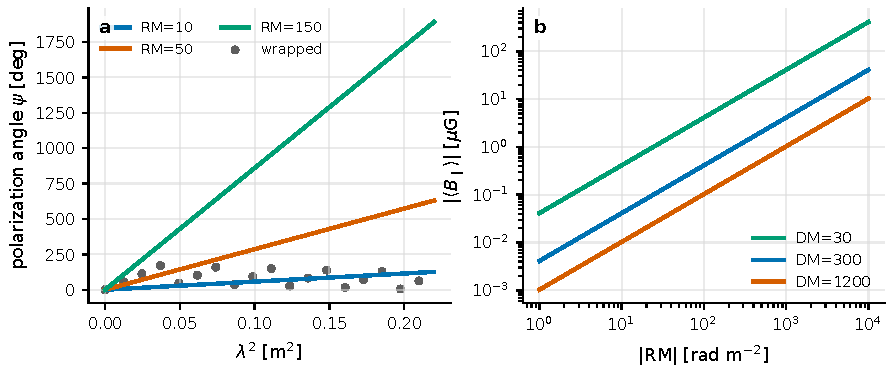
\includegraphics[width=0.94\linewidth]{figures/generated/chapter_14/ch14_faraday_rotation.pdf}
\caption{Two readings of Faraday rotation. The left panel is the linear relation \(\psi=\psi_0+{\rm RM}\,\lambda^2\); the black dots remind us that the polarization angle can only be measured modulo \(\pi\), and narrowband data easily suffer an \(n\pi\)-wrapping ambiguity (a sufficiently wide \(\lambda^2\) coverage is needed to fix a unique slope). The right panel plots \(\langle B_\parallel\rangle=1.232\,{\rm RM}/{\rm DM}\) as a function of RM: the same RM represents a stronger mean field in a tenuous, low-DM medium.}
\label{fig:e21-faraday}
\end{figure}

For coherence and polarization measurements, the implication of Faraday rotation is direct: if your receiving bandwidth spans a non-negligible range of \(\lambda^2\) and RM is large, then the polarization angles of different frequencies within the band are rotated to different directions, and averaging them without correction will \textbf{dilute} (depolarize) the net polarization: this is precisely the version, in the polarization dimension, of the spirit of Chapter~\ref{chap:e02}, ``phase misalignment within the bandwidth weakens coherent superposition.'' The remedy is to first measure RM, rotate the polarization angle of each channel back to its intrinsic value, and then superpose coherently.

\section{Scattering and scintillation: how multiple paths scramble coherence}
\label{sec:e21-scattering}

Both dispersion and Faraday rotation are very ``gentlemanly'': they only give different frequencies and different polarizations a definite relative delay or rotation, which is undone by removal. Scattering is different: it acts on the \textbf{direction} and on \textbf{coherence} itself. The interstellar electron density is not smooth, and turbulence stirs up density fluctuations on all scales; these fluctuations, like ground glass, crumple the flat wavefront. The consequences of the crumpling are threefold: the source image is angularly broadened (angular broadening), a narrow pulse is dragged out into a long tail (temporal broadening), and the intensity scintillates with time and frequency (scintillation): the three things are in fact one and the same thing projected onto angle, time, and frequency.

Let us first look at the temporal tail. After the wavefront is crumpled, light can reach us along many slightly longer paths, equivalent to an instantaneous signal at the source being spread over a short interval of time. In the simplest \textbf{single-thin-screen} approximation, the observed pulse is the convolution of the source pulse with an arrival-time kernel:
\begin{equation}
  I_{\rm obs}(t)
  =
  \int I_{\rm src}(t')\,P(t-t')\,{\rm d}t',
  \qquad
  P(t)=\frac{1}{\tau_{\rm sc}}\exp\!\left(-\frac{t}{\tau_{\rm sc}}\right)H(t).
  \label{eq:e21-scattering-convolution}
\end{equation}
\begin{formulaexplain}
\(I_{\rm obs}\) is the observed intensity, \(I_{\rm src}\) is the source-end intensity, \(P(t)\) is the scattering arrival-time kernel, \(\tau_{\rm sc}\) is the scattering broadening timescale, and \(H(t)\) is the step function. The kernel is a \textbf{one-sided} exponential: light can only be \textbf{delayed} by taking a detour, never arrive early, so a symmetric narrow pulse comes out as a ``steep-rise, slow-decay'' long tail.
\end{formulaexplain}
Here \(\tau_{\rm sc}\) is in seconds (or milliseconds), the \(1/e\) decay time of the long tail. A real line of sight may have multiple screens, anisotropic scattering, and a finite source size; the one-sided exponential is only the most commonly used low-order model. \(\tau_{\rm sc}\) depends strongly on frequency:
\begin{equation}
  \tau_{\rm sc}\propto \nu^{-\alpha}.
  \label{eq:e21-scattering-power}
\end{equation}
\begin{formulaexplain}
\(\alpha\) is the frequency index of scattering. Thin-screen theory for Kolmogorov turbulence gives \(\alpha\simeq4.4\), while the empirical average of multi-frequency pulsar samples is closer to \(3.9\pm0.2\). With so steep an index, going to lower frequency makes the scattering tail explode in length. This is the most troublesome enemy of low-frequency pulse searches.
\end{formulaexplain}
Empirically, a common fitting formula linking \(\tau_{\rm sc}\) to DM and frequency is used:
\begin{equation}
  \log_{10}\!\left(\frac{\tau_{\rm sc}}{{\rm ms}}\right)
  =
  -6.46
  +0.154\log_{10}{\rm DM}
  +1.07(\log_{10}{\rm DM})^2
  -3.86\log_{10}\!\left(\frac{\nu}{\rm GHz}\right),
  \label{eq:e21-bhat-scattering}
\end{equation}
\begin{formulaexplain}
This is an empirical scattering relation (DM in units of \({\rm pc\,cm^{-3}}\)), suitable only for order-of-magnitude estimates. The quadratic term \((\log_{10}{\rm DM})^2\) reflects high-DM lines of sight passing through more turbulence; \(-3.86\log_{10}\nu\) is the logarithmic version of Equation~\eqref{eq:e21-scattering-power}. The turbulent structure of a real line of sight brings a scatter far exceeding an order of magnitude.
\end{formulaexplain}
Plugging in numbers: at \({\rm DM}=300\,{\rm pc\,cm^{-3}}\), \(\nu=1.4\,{\rm GHz}\) it gives a broadening of order milliseconds; dropping to \(0.6\,{\rm GHz}\), by that \(\nu^{-3.86}\), the broadening grows to a dozen milliseconds or more. Scattering drags a millisecond pulse into a tens-of-milliseconds mush, and the microstructure is thereby lost: this is pure ``contamination.''

Now to the most crucial connection between this chapter and coherence. The temporal tail is, in the frequency domain, equivalent to a \textbf{decorrelation bandwidth} \(\Delta\nu_d\), the width over which the scintillation pattern still ``remembers itself'' in frequency:
\begin{equation}
  \tau_{\rm sc}\simeq \frac{C_1}{2\pi\,\Delta\nu_d}.
  \label{eq:e21-decorrelation-bandwidth}
\end{equation}
\begin{formulaexplain}
\(\Delta\nu_d\) is the decorrelation bandwidth of scintillation, and \(C_1\) is a constant related to the geometry and scattering spectrum (usually \(\sim1\)). It is the scattering version of the uncertainty relation ``time width is inversely proportional to spectral width'' of Chapter~\ref{chap:e02}: the longer the multipath delay (large \(\tau_{\rm sc}\)), the narrower the correlated bandwidth \(\Delta\nu_d\) in frequency.
\end{formulaexplain}
This expression lays bare the meaning of scattering for coherence measurement. Recall Chapter~\ref{chap:e02}: the coherence time \(\tau_c\simeq1/\Delta\nu\). Scattering is equivalent to superimposing an extra, random phase structure on the signal, whose ``coherence bandwidth'' is precisely \(\Delta\nu_d\). When scattering is strong and \(\Delta\nu_d\) is only a few tens of kHz, doing coherent superposition over a broadband of several hundred MHz amounts to forcing together thousands of mutually incoherent patches, the net coherence is diluted almost to zero. Conversely, scattering also \textbf{encodes} information: when scattering is weak and \(\Delta\nu_d\) is measurable, the drift of scintillation patches with time and frequency can be inverted for the velocity of the scattering screen, the distance from the screen to us, and even the angular size of the source, an ``interstellar scintillation telescope,'' whose effective angular resolution can reach microarcseconds, far surpassing any single-aperture telescope. These are the two faces of scattering: both the ground glass that smears out coherence, and a free ultra-high-resolution probe.

\begin{figure}[tbp]
\centering
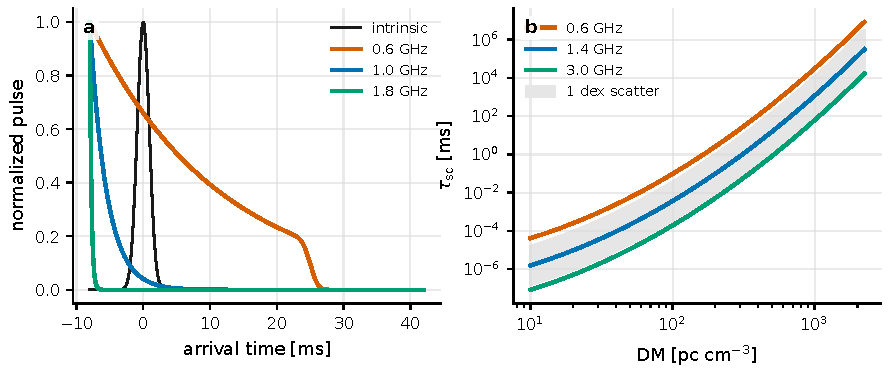
\includegraphics[width=0.94\linewidth]{figures/generated/chapter_14/ch14_scattering_broadening.pdf}
\caption{Interstellar scattering drags a short pulse into an arrival-time distribution with a long tail. The left panel convolves a narrow Gaussian pulse with a one-sided exponential kernel; the lower the frequency, the longer \(\tau_{\rm sc}\propto\nu^{-4}\) stretches the tail, and the symmetry of the pulse is utterly destroyed. The right panel uses the empirical relation to plot the variation of \(\tau_{\rm sc}\) with DM and frequency, with the gray band showing the common scatter of over an order of magnitude at fixed DM.}
\label{fig:e21-scattering}
\end{figure}

In passing: plasma does not only ``crumple'' the wavefront; a transverse gradient in the electron column density can also \textbf{refract} light like a (frequency-dependent) lens, with the low frequencies deflected more strongly, potentially causing narrowband magnification, caustics, or multiple images. This reminds us that even after the \(\nu^{-2}\) dispersion has been cleaned out, residual structure in the dynamic spectrum may still be a product of propagation rather than an intrinsic variation of the source \citep{1998ApJ...496..253C,2014MNRAS.437.2180E}. When doing millimeter-wave VLBI toward the Galactic center, this strong scattering screen is especially troublesome: to image the event-horizon scale of Sgr A*, one must simultaneously handle the intrinsic structure, the scattering blur, and the temporal variation \citep{2008Natur.455...78D,2022ApJ...930L..14E,2022ApJ...930L..15E}.

\section{Dust: a loss channel with wavelength selectivity}
\label{sec:e21-dust}

Plasma acts mainly on radio and arrival time; dust acts mainly on the optical and infrared \textbf{flux and color}. For optical photons, dust grains are like a picky loss channel: they absorb and scatter selectively by wavelength, with short waves (blue light) lost more than long waves (red light), so starlight passing through dust becomes both dimmer and redder. The most basic extinction relation is
\begin{equation}
  F_{\lambda,{\rm obs}}
  =
  F_{\lambda,{\rm int}}\,10^{-0.4A_\lambda},
  \label{eq:e21-extinction-flux}
\end{equation}
\begin{formulaexplain}
\(F_{\lambda,{\rm int}}\) is the intrinsic flux, \(F_{\lambda,{\rm obs}}\) is the extincted flux, and \(A_\lambda\) is the extinction at wavelength \(\lambda\), in magnitudes (mag). Magnitude is inherently a logarithmic scale, so \(A_\lambda\) suppresses the flux in the exponent in the form \(10^{-0.4A_\lambda}\): \(A_\lambda=1\) magnitude corresponds to the flux dropping to about \(0.40\) times, and \(A_\lambda=2.5\) to about \(0.10\) times.
\end{formulaexplain}
The variation of extinction with wavelength is summarized by two quantities that characterize its degree of ``reddening'':
\begin{equation}
  E(B-V)=A_B-A_V,
  \qquad
  R_V=\frac{A_V}{E(B-V)}.
  \label{eq:e21-rv-definition}
\end{equation}
\begin{formulaexplain}
\(E(B-V)\) is the difference in extinction between the blue band \(B\) and the visible band \(V\), called the \textbf{color excess}, measuring how much the starlight has been ``reddened''; \(R_V=A_V/E(B-V)\) is the ratio of total extinction to selective reddening, measuring the ``grayness'' of the extinction curve. The larger \(R_V\), the flatter (grayer) the curve, indicating that larger dust grains dominate.
\end{formulaexplain}
Term by term: \(A_B,A_V\) are the extinctions in the \(B\) and \(V\) bands (each in mag), and \(E(B-V)\) is also in mag. The Galactic mean is \(R_V\simeq3.1\), mostly \(2.5\text{--}3.5\) in the diffuse interstellar medium, and can reach above \(5\) in dense molecular clouds (large grains make the extinction grayer). The Cardelli--Clayton--Mathis (CCM) extinction law compresses the mean infrared, optical, and ultraviolet curves into a one-parameter family parameterized by \(R_V\); Fitzpatrick further pointed out that real lines of sight still have marked scatter, especially in the strength of the \(2175\,\text{\AA}\) ultraviolet bump (UV bump) and the far-ultraviolet upturn \citep{1989ApJ...345..245C,1999PASP..111...63F,2003ARA&A..41..241D}.

Here there is an \textbf{error floor} crucial for transient and polarization measurements. If you correct a blue source with \(E(B-V)=0.2\) magnitude using only a mean extinction law, a residual error of \(0.1\) magnitude at the ultraviolet end is nothing unusual, and for the polarization angle, the color temperature, and the early spectral energy distribution (SED) of a transient source, this is the dominant systematic error. In other words, dust not only dims the source, it also injects a non-negligible uncertainty into the measurement of ``color.''

Dust grains are mostly non-spherical, and they partly align their orientations in the interstellar magnetic field, so they absorb starlight of different vibration directions unequally, injecting a little \textbf{linear polarization} into the transmitted starlight. Its wavelength dependence is described by the empirical Serkowski relation:
\begin{equation}
  \frac{P(\lambda)}{P_{\max}}
  =
  \exp\!\left[-K\ln^2\!\left(\frac{\lambda_{\max}}{\lambda}\right)\right].
  \label{eq:e21-serkowski}
\end{equation}
\begin{formulaexplain}
\(P(\lambda)\) is the degree of linear polarization caused by dust, \(P_{\max}\) is the peak polarization, \(\lambda_{\max}\) is the peak wavelength, and \(K\) controls the curve width. It is a Gaussian-type peak in the variable \(\ln(\lambda_{\max}/\lambda)\): the polarization is maximal at \(\lambda_{\max}\) and decays symmetrically to both sides. The peak position \(\lambda_{\max}\) is sensitive to grain size.
\end{formulaexplain}
Empirically \(\lambda_{\max}\approx0.55\,\mu{\rm m}\), and the upper limit of the peak degree of polarization is about \(P_{\max}\lesssim9\,E(B-V)\%\) (i.e.\ at most about 0.9\% polarization per 0.1 mag of color excess). This upper limit is not reached on every line of sight; it is affected by grain shape, alignment efficiency, variations of the magnetic-field direction along the line of sight, and the superposition of multiple cloud layers \citep{1975ApJ...196..261S,2015ARA&A..53..501A}. For any experiment seeking to measure the source's intrinsic polarization, this dust polarization is a foreground that must be subtracted first.

Dust can also ``replay'' a brief burst as a \textbf{light echo} or an X-ray halo: the light of the burst is scattered into our line of sight by dust en route, and because it took a detour, it arrives later than the direct light. If the dust screen is located at a fraction \(x\) of the source-to-observer distance and the scattering angle is \(\theta\), the geometric delay is approximately
\begin{equation}
  \Delta t_{\rm dust}
  \simeq
  \frac{D_s}{2c}\,\frac{x}{1-x}\,\theta^2 .
  \label{eq:e21-dust-delay}
\end{equation}
\begin{formulaexplain}
\(\Delta t_{\rm dust}\) is the geometric delay of dust scattering, \(D_s\) is the source distance, \(x\) is the relative position of the dust screen (\(0\) at the source, \(1\) at the observer), and \(\theta\) is the scattering angle. The delay is proportional to \(\theta^2\), so an angularly resolved light echo can invert the geometric position of the dust: the expansion of the delay with scattering angle is a distance-measuring ruler.
\end{formulaexplain}
In order of magnitude, for a Galactic source an arcsecond-scale scattering angle gives a delay of hours to days; for an extragalactic source, the geometric position of the dust and the telescope angular resolution must enter the model together. This is again a case of ``contamination is encoding'': the dust that originally blocked light, by the delay--angle relation, becomes a probe for measuring the three-dimensional dust distribution around the burst.

\begin{figure}[tbp]
\centering
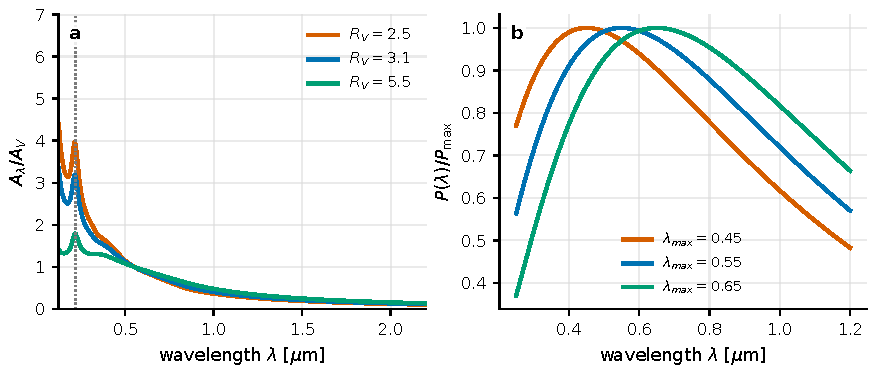
\includegraphics[width=0.94\linewidth]{figures/generated/chapter_14/ch14_dust_extinction_polarization.pdf}
\caption{Dust simultaneously changes a photon's flux, color, and polarization. The left panel is the CCM mean extinction curve; the larger \(R_V\), the ``grayer'' from optical to near-infrared; the ultraviolet bump near \(0.2175\,\mu{\rm m}\) is an important diagnostic of small grains and carbonaceous material. The right panel is the Serkowski polarization curve; the shift of the peak position \(\lambda_{\max}\) reflects changes in grain size and the alignment environment.}
\label{fig:e21-dust}
\end{figure}

\section{Gravitational lensing: turning one path into many}
\label{sec:e21-lensing}

The previous three rewriters all came from real media: electrons, magnetic fields, dust grains. The last one is different: gravitational lensing comes from \textbf{curved spacetime} itself. It does not change the frequency of a photon (no dispersion), but it changes the path, direction, and arrival time of the light. For the event table, the core action of a lens can be summarized in one sentence: \textbf{one source event can become multiple images, multiple arrival times, and multiple magnification weights}.

In the thin-lens approximation, the source's true direction and the image directions we see are connected by the lens equation:
\begin{equation}
  {\boldsymbol\beta}
  =
  {\boldsymbol\theta}
  -
  {\boldsymbol\alpha}({\boldsymbol\theta}),
  \label{eq:e21-lens-equation}
\end{equation}
\begin{formulaexplain}
\({\boldsymbol\beta}\) is the true angular position of the source, \({\boldsymbol\theta}\) is the angular position of the image, and \({\boldsymbol\alpha}\) is the reduced deflection angle, all in angular units (rad or arcsec). The equation says: the image direction \({\boldsymbol\theta}\) we see equals the true direction \({\boldsymbol\beta}\) plus the angle by which the mass bends the light. Given \({\boldsymbol\beta}\), this equation can have \textbf{multiple} solutions \({\boldsymbol\theta}\): those are the multiple images.
\end{formulaexplain}
The natural angular scale of the deflection is given by the Einstein angle. For a point-mass lens,
\begin{equation}
  \theta_E
  =
  \left(
  \frac{4GM}{c^2}
  \frac{D_{ls}}{D_lD_s}
  \right)^{1/2}.
  \label{eq:e21-einstein-angle}
\end{equation}
\begin{formulaexplain}
\(\theta_E\) is the Einstein angle, \(M\) is the lens mass, \(G\) is the gravitational constant, and \(D_l,D_s,D_{ls}\) are the angular diameter distances from observer to lens, to source, and from lens to source, respectively. The core factor \(4GM/c^2\) is the signature of general-relativistic light deflection (twice the Newtonian prediction). \(\theta_E\) sets the natural scale of the multiple-image separation and of microlensing.
\end{formulaexplain}
Two real orders of magnitude separate the two kinds of lensing. \(M=1\,M_\odot\), on Galactic-scale geometry, gives a \(\theta_E\) of order milliarcseconds (mas), too small to separate two images, so one can only see brightness fluctuating with time; this is \textbf{microlensing}: a foreground star drifting in front of a background star, magnifying it briefly. And a galaxy lens of \(M\sim10^{11}\text{--}10^{12}\,M_\odot\) gives a \(\theta_E\) of order arcseconds (arcsec), with the multiple images cleanly separated; this is \textbf{strong lensing}. The magnification is determined by the Jacobian determinant of the mapping from the image plane to the source plane:
\begin{equation}
  \mu
  =
  \frac{1}{\det\!\left(\partial{\boldsymbol\beta}/\partial{\boldsymbol\theta}\right)}.
  \label{eq:e21-magnification}
\end{equation}
\begin{formulaexplain}
\(\mu\) is the magnification, and the denominator is the Jacobian determinant from the image plane \({\boldsymbol\theta}\) to the source plane \({\boldsymbol\beta}\). The lens neither creates nor absorbs photons; it merely redistributes solid angle, so by whatever factor the area is stretched, that is how much the brightness is magnified. When the determinant tends to zero, the image plane is stretched infinitely and the magnification diverges: that curve is called a caustic.
\end{formulaexplain}
Near a caustic \(|\mu|\) can be very large (in theory divergent), but the finite source size, microlensing, dust, and time sampling all push down the peak magnification actually observable. The physics of this expression is very clean: magnification is a geometric redistribution, not a creation of energy out of nothing.

Now to the deepest, and most on-theme, point of lensing: the \textbf{time delay}. The different images travel paths of different length and pass through gravitational potentials of different depth, so their light does not arrive simultaneously. The arrival time is governed by the Fermat potential:
\begin{equation}
  t({\boldsymbol\theta},{\boldsymbol\beta})
  =
  \frac{D_{\Delta t}}{c}
  \left[
  \frac{1}{2}\,|{\boldsymbol\theta}-{\boldsymbol\beta}|^2
  -
  \psi({\boldsymbol\theta})
  \right],
  \qquad
  D_{\Delta t}
  =
  (1+z_l)\frac{D_lD_s}{D_{ls}} .
  \label{eq:e21-fermat-delay}
\end{equation}
\begin{formulaexplain}
\(t\) is the relative arrival time, the first term in the brackets \(\tfrac12|{\boldsymbol\theta}-{\boldsymbol\beta}|^2\) is the \textbf{geometric path difference} (the extra time spent taking a detour), and the second term \(\psi\) is the \textbf{gravitational potential delay} (the Shapiro delay, light ``travels more slowly'' in a deep potential well). \(D_{\Delta t}\) is the time-delay distance, and \(z_l\) is the lens redshift. The real images appear at the \textbf{stationary points} (minimum, maximum, or saddle) of this time surface, this is precisely Fermat's principle: ``light takes the path of extremal time.''
\end{formulaexplain}
The geometric origin of the time delay is hidden in the tug-of-war between these two terms: the farther one deviates from the source direction, the larger the geometric term (arriving late), but usually the closer to the mass and the deeper the potential well (the Shapiro term is also changing). The observed delay of two images is precisely the difference of their Fermat potentials:
\begin{equation}
  \Delta t_{AB}
  =
  \frac{D_{\Delta t}}{c}\,
  \Delta\phi_{AB}.
  \label{eq:e21-time-delay-distance}
\end{equation}
\begin{formulaexplain}
\(\Delta t_{AB}\) is the arrival-time difference between image \(A\) and image \(B\), and \(\Delta\phi_{AB}\) is the Fermat-potential difference of the two (computed from the lens mass model). Measuring \(\Delta t_{AB}\), and having a lens model that gives \(\Delta\phi_{AB}\), one can invert for \(D_{\Delta t}\), and since \(D_{\Delta t}\propto 1/H_0\), the time delay directly measures the Hubble constant.
\end{formulaexplain}
Order of magnitude: the \(\Delta t_{AB}\) of galaxy strong lensing is often days to months, and in a few cases up to years. Note that it is only about \(10^{-11}\) of \(D_{\Delta t}/c\) (because \(\Delta\phi_{AB}\) is a small number), so every bit of error in the lens potential, the external convergence, the mass-sheet degeneracy, and the light-curve sampling flows straight into the error budget of \(H_0\). Refsdal pointed out as early as 1964 that the time delay of multiple images can measure \(H_0\); modern time-delay cosmography, relying on multi-year monitoring, high-resolution imaging, lens-galaxy velocity dispersion, and environment modeling, has turned this idea into a measurement of \(H_0\) independent of the cosmic microwave background \citep{1964MNRAS.128..295R,1964MNRAS.128..307R,1986ApJ...310..568B,2016A&ARv..24...11T}. This is yet another beautiful encoding of the chapter: the time delay was originally the contamination of ``the same source copied into several time-offset replicas,'' and it turns out the expansion rate of the universe is locked in that time offset.

\begin{figure}[tbp]
\centering
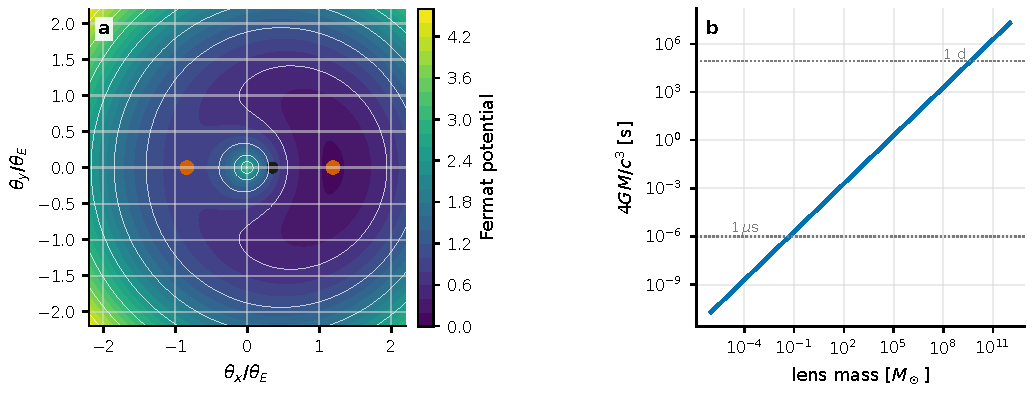
\includegraphics[width=0.94\linewidth]{figures/generated/chapter_14/ch14_lensing_time_delay.pdf}
\caption{The two scales of strong lensing. The left panel is the Fermat arrival-time surface of a point-mass lens, with the black dot the source position and the two orange dots the image positions; the images appear precisely at the stationary points of the arrival-time surface (minimum and saddle). The right panel gives the basic delay scale \(4GM/c^3\): stellar-mass lenses fall in microseconds to milliseconds, and galaxy and cluster lenses naturally enter the day-to-year time domain.}
\label{fig:e21-lensing}
\end{figure}

\paragraph{When wavelength cannot be ignored: from rays to diffraction}
\label{sec:e21-wavelensing}

The above treated light as ``rays,'' by default assuming that multiple paths can be cleanly separated. But when the wavelength is comparable to the time delay induced by the lens, geometric optics fails, and one must return to the \textbf{wave} picture, just as Chapter~\ref{chap:e02} repeatedly stressed, waves diffract and interfere. The criterion is a dimensionless frequency:
\begin{equation}
  w
  =
  \frac{8\pi GM(1+z_l)f}{c^3}.
  \label{eq:e21-wave-lensing-w}
\end{equation}
\begin{formulaexplain}
\(w\) is the dimensionless frequency of wave lensing, \(M\) is the lens mass, \(f\) is the wave frequency, and \(z_l\) is the lens redshift. \(w\) compares the wave period \(1/f\) with the time-delay scale \(\sim GM/c^3\) induced by the lens: when \(w\gg1\) the delay is far longer than the period and one returns to geometric optics; when \(w\lesssim1\) the delay is less than one period and diffraction cannot be neglected.
\end{formulaexplain}
In the geometric regime (\(w\gg1\)), multiple images can be separated and can coherently interfere like a double slit; in the diffraction regime (\(w\lesssim1\)), the caustics are smeared out and the magnification can no longer simply add the geometric images. The frequency-domain waveform is written as
\begin{equation}
  \tilde h_L(f)=F(f)\,\tilde h(f),
  \label{eq:e21-wave-amplification}
\end{equation}
\begin{formulaexplain}
\(\tilde h(f)\) is the unlensed frequency-domain waveform, \(\tilde h_L(f)\) is the lensed one, and \(F(f)\) is the complex amplification factor. It is a complex number, so it simultaneously carries \textbf{amplitude magnification} (modulus) and \textbf{phase delay} (argument), able to create frequency-dependent interference fringes.
\end{formulaexplain}
If the two paths have a delay \(\Delta t\), the two complex amplitudes add, and the beating with frequency gives a frequency-domain fringe spacing
\begin{equation}
  \Delta f \simeq \frac{1}{\Delta t}.
  \label{eq:e21-lensing-fringe-spacing}
\end{equation}
\begin{formulaexplain}
\(\Delta f\) is the spacing of the frequency-domain interference fringes, and \(\Delta t\) is the time delay of the two paths. This is yet another appearance of that old Fourier rule (Chapter~\ref{chap:e02}): two replicas separated in time by \(\Delta t\) weave, in the spectrum, fringes of spacing \(1/\Delta t\). The longer the path delay, the denser the frequency-domain oscillation.
\end{formulaexplain}
Plugging in numbers: \(\Delta t=2\,{\rm ms}\) gives a fringe spacing of \(\Delta f\approx500\,{\rm Hz}\). For the electromagnetic-wave frequencies of the optical and radio, \(f\sim10^{14}\) or \(10^{9}\,{\rm Hz}\), the \(w\) of an ordinary stellar- or galaxy-mass lens is astonishingly large, and geometric optics is almost perfect; but for gravitational waves in the LISA band (\(f\sim10^{-3}\,{\rm Hz}\)) with a lens of \(10^{6}\text{--}10^{9}\,M_\odot\), the wave-optics effect of \(w\sim1\) really does fall into the observing band \citep{2003ApJ...595.1039T}. This is the most direct interface between lensing and the quantum-optics through-line of this book: the interference after lensing is essentially the coherent superposition of the same source field along two paths, and what is read is still the phase.

\begin{figure}[tbp]
\centering
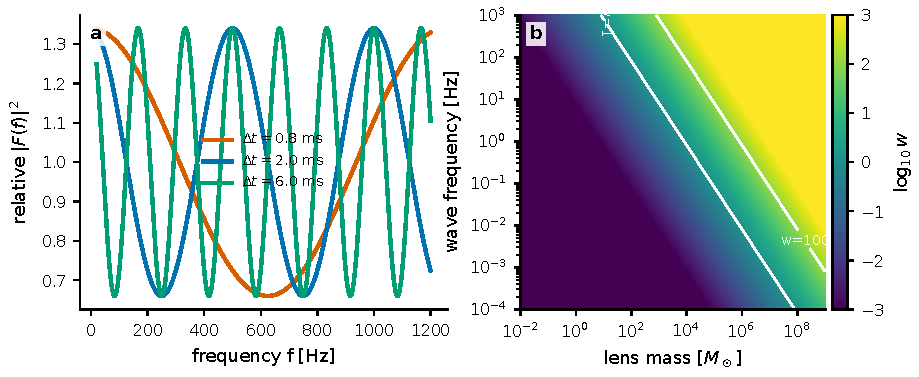
\includegraphics[width=0.94\linewidth]{figures/generated/chapter_14/ch14_wave_lensing_interference.pdf}
\caption{Wave-optics lensing transcribes the time delay into frequency-domain fringes. The left panel plots the oscillation of the relative amplification factor under different path delays, with fringe spacing \(\Delta f\simeq1/\Delta t\). The right panel gives the order of magnitude of \(w=8\pi GMf/c^3\); the region near the white line \(w=1\) is the transition between diffraction and geometric optics, and for \(w\gtrsim100\) one can usually treat the images as independent paths.}
\label{fig:e21-wave-lensing}
\end{figure}

\section{Contamination or encoding: what propagation means for coherence and timing}
\label{sec:e21-correlation}

Having gone around a full circle, we return to the book's through-line: the correlation function. The previous sections all rewrote the \textbf{labels of individual events}; this section looks at how they rewrite the \textbf{correlation between events}. The core insight is simple: multipath propagation (scattering, lensing) reshuffles the intensity correlation, because the two fluctuations observed need not come from the same source-end instant: they may be two replicas of the same source-end structure, arriving time-offset along different paths.

Writing the resolvable multipath as a string of delta impulse responses:
\begin{equation}
  h(t)=\sum_i \sqrt{\mu_i}\,e^{i\varphi_i}\,\delta(t-t_i),
  \label{eq:e21-multipath-impulse}
\end{equation}
\begin{formulaexplain}
\(h(t)\) is the multipath impulse response, \(\mu_i\) is the magnification of the \(i\)-th path, \(\varphi_i\) is its phase, and \(t_i\) is its arrival delay. Each delta function is a resolvable path: it is the concrete form of the abstract \(h_{ij}\) in Equation~\eqref{eq:e21-channel-time} in the ``discrete multiple-image'' case.
\end{formulaexplain}
If the phases \(\varphi_i\) are averaged out over the observing bandwidth or the source size (the common situation when coherence is diluted), the observed intensity is the sum of the path intensities weighted by magnification and offset in time:
\begin{equation}
  I_{\rm obs}(t)
  =
  \sum_i \mu_i\,I_{\rm src}(t-t_i).
  \label{eq:e21-multipath-intensity}
\end{equation}
\begin{formulaexplain}
\(I_{\rm obs}\) is the observed intensity, and \(I_{\rm src}\) is the source-end intensity. After the phase is averaged, the interference terms vanish, leaving only the sum of the path intensities weighted by \(\mu_i\), so one change at the source is repeated once at each of several different delays \(t_i\).
\end{formulaexplain}
Autocorrelating the intensity fluctuation \(\delta I=I-\langle I\rangle\), one can see how the ``echo'' enters the correlation function:
\begin{equation}
  C_{\rm obs}(\tau)
  =
  \left\langle
  \delta I_{\rm obs}(t)\,
  \delta I_{\rm obs}(t+\tau)
  \right\rangle
  =
  \sum_{ij}\mu_i\mu_j\,
  C_{\rm src}\!\left(\tau+t_i-t_j\right).
  \label{eq:e21-correlation-echo}
\end{equation}
\begin{formulaexplain}
\(C_{\rm obs}\) is the observed intensity autocorrelation, and \(C_{\rm src}\) is the source-end autocorrelation. The double sum means that \textbf{every pair of paths} contributes a correlation echo, the echo appearing at \(\tau=t_j-t_i\) with weight \(\mu_i\mu_j\). One peak originally is copied into a comb of echo peaks.
\end{formulaexplain}
This expression makes clear the effect of propagation on the intensity-correlation toolkit of Chapter~\ref{chap:e08}: \textbf{a correlation peak no longer uniquely corresponds to source-end physics}. The \(g^{(2)}(0)\) peak of thermal light, the microstructure of pulsar giant pulses, the narrowband scintillation of FRBs, and the delay of lensed multiple images can all fall into this framework, but their coherence times, bandwidths, and statistical distributions are each different. Seeing a single correlation peak is not enough to determine its physical origin. The prerequisites for using Equation~\eqref{eq:e21-correlation-echo} are hard: the source itself must have measurable fast structure, the propagation path must be stable, the observing time must be long enough, and the background and selection function must have been modeled. This is precisely the payoff of the ``channel with memory'' viewpoint: it forces you, before interpreting any correlation peak, to first ask, ``could this be just a late-arriving path?''

Propagation effects also delimit a class of quantum-foundations experiments. The so-called cosmic Bell test uses entangled photon pairs to make measurements at two stations, each side choosing measurement settings \(a,a'\) and \(b,b'\), and constructs the CHSH combination:
\begin{equation}
  S
  =
  E(a,b)+E(a,b')+E(a',b)-E(a',b'),
  \qquad
  |S|\le 2 .
  \label{eq:e21-chsh}
\end{equation}
\begin{formulaexplain}
\(S\) is the CHSH combination, and \(E(a,b)\) is the correlation expectation of the two stations' measurement results under given settings. Local hidden-variable theories require \(|S|\le2\); quantum mechanics can violate it up to \(2\sqrt2\). The distinctive feature of a cosmic Bell experiment is using \textbf{astronomical photons} to decide the settings \(a,b\) in real time.
\end{formulaexplain}
Its point is not that the celestial photons themselves are in an entangled state, but to use the light of distant celestial objects to \textbf{choose the measurement settings in real time}: the Galactic-star version uses starlight color to generate \(a,b\), pushing the possible ``common cause'' back to hundreds or thousands of years ago; the quasar version is even more extreme, pushing the common past of the freedom-of-choice loophole back to the early universe \citep{2017PhRvL.118f0401H,2018PhRvL.121h0403R} (Figure~\ref{fig:e21-cosmic-bell}). And this requires everything in this chapter: the arrival time of the starlight must have the atmospheric delay subtracted (the time synchronization of Chapter~\ref{chap:e13}), the color must have the dust reddening subtracted, radio quasars must also account for dispersion and scattering, and the instrumental electronic delay must enter the experimental timing term by term: every absorption, reddening, dispersion, and delay in propagation must be placed into the experiment's causal timing, otherwise the loophole cannot be sealed tight.

\begin{figure}[tbp]
\centering
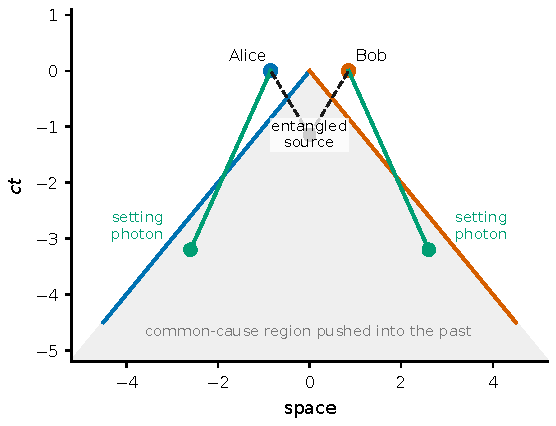
\includegraphics[width=0.72\linewidth]{figures/generated/chapter_14/ch14_cosmic_bell_lightcones.pdf}
\caption{The light-cone structure of a cosmic Bell experiment. The entangled source emits photon pairs in the local experiment, and the measurement settings of Alice and Bob are decided in real time by photons from distant stars or quasars; the earlier the emission events of these setting photons and the greater their directional separation, the larger the spacetime region from which a ``common cause'' can be excluded (the gray region in the figure). A real experiment must also add, term by term, atmospheric propagation, dust reddening, detector response, and electronic delay. This is precisely where each effect of this chapter must enter the experimental timing.}
\label{fig:e21-cosmic-bell}
\end{figure}

Finally, let us regard these ``ordinary'' propagation effects as the \textbf{error floor} of new-physics searches. Axion-like particles can let photons convert in a magnetic field and cause spectral absorption, cosmic birefringence rotates polarization, and dark-matter substructure can rewrite the magnification and time delay of a lens. All these fascinating explanations must first be compared with plasma dispersion, dust, conventional lensing, and instrumental terms within the same model. Only when a residual signal simultaneously withstands the four tests of time, frequency, polarization, and angular position, and no known propagation effect can subtract it away, does it qualify to queue up as a candidate for new physics. This is the most practical conclusion of the chapter's theme ``contamination is background, encoding is signal'': first characterize this channel with memory to the end, and what remains is what truly belongs to the source, and even to new physics.

\section*{Chapter Summary}
\addcontentsline{toc}{section}{Chapter Summary}

\begin{itemize}
\item \textbf{Propagation is a channel with memory, not gray glass.} Equation~\eqref{eq:e21-channel-time} writes the source-end field to detector event as a convolution: the medium rewrites each photon's time, frequency, polarization, and direction label, not merely multiplies by a constant.
\item \textbf{The \(\nu^{-2}\) law of dispersion is derived step by step from the group velocity.} Refractive index \(\to\) group velocity \(v_g\approx c(1-\omega_p^2/2\omega^2)\) \(\to\) integration along the line of sight, giving \(\Delta t\propto{\rm DM}/\nu^2\) (Equation~\eqref{eq:e21-dm-delay}). The root cause of low frequency arriving late is ``the low-frequency group velocity is slower.'' DM is the electron column density, and the DM--redshift relation of FRBs can weigh the cosmic baryons.
\item \textbf{Faraday rotation adds the magnetic-field direction to dispersion.} The slope of the polarization angle against \(\lambda^2\) is RM, whose integrand \(n_e B_\parallel\) is signed, so RM/DM gives the electron-weighted mean magnetic field (Equation~\eqref{eq:e21-bfield-rm-dm}), but only when the two are cospatial does it have direct physical meaning.
\item \textbf{Scattering scrambles coherence, and also offers ultra-high resolution for free.} A one-sided exponential kernel drags a narrow pulse into a long tail (\(\tau_{\rm sc}\propto\nu^{-4}\)), and the decorrelation bandwidth \(\Delta\nu_d\simeq1/2\pi\tau_{\rm sc}\) (Equation~\eqref{eq:e21-decorrelation-bandwidth}) determines whether broadband coherent superposition is diluted; under weak scattering, scintillation can conversely be inverted for the screen velocity, screen distance, and source angular size.
\item \textbf{Dust is a loss channel with wavelength selectivity.} Extinction \(F_{\rm obs}=F_{\rm int}10^{-0.4A_\lambda}\) makes the source both dimmer and redder, and \(R_V\) sets the grayness of the curve; the residual of the mean extinction law is the dominant systematic of polarization and the early SED; Serkowski polarization and dust light echoes are both foregrounds that must be subtracted first.
\item \textbf{Gravitational lensing turns one path into many.} The Einstein angle sets the scale (stellar mass mas, galaxy arcsec), the magnification is the reciprocal of the geometric Jacobian, and the time delay is determined by the geometric term plus the Shapiro term of the Fermat potential (Equation~\eqref{eq:e21-fermat-delay}), and it measures the Hubble constant because \(D_{\Delta t}\propto1/H_0\). When wavelength cannot be ignored, use the dimensionless frequency \(w\) to judge the geometric/diffraction regime.
\item \textbf{Contamination is encoding.} Multipath copies one source-end fluctuation into a correlation echo (Equation~\eqref{eq:e21-correlation-echo}), so a correlation peak does not uniquely correspond to source-end physics; these ordinary effects in turn constitute the timing constraints of the cosmic Bell test and the error floor of new-physics searches.
\end{itemize}

\medskip
\noindent\textbf{Questions to Ponder.}
\begin{itemize}
\item If an FRB is measured to have a delay of \(1.2\,{\rm s}\) between \(1.4\,{\rm GHz}\) and \(0.8\,{\rm GHz}\), roughly what is its DM? (Invert using Equation~\eqref{eq:e21-dispersion-delay}.) If this line of sight is mainly within the Galaxy, is it reasonable compared with the typical high-Galactic-latitude value?
\item For the same RM, if there is a field reversal along the line of sight, will the RM you measure be larger or smaller? Why is DM unaffected by this reversal?
\item The time delay of the two images of a galaxy strong lens is measured to be \(30\) days, and the lens model gives \(\Delta\phi_{AB}\). To measure \(H_0\) to 3\% precision, which links in Equation~\eqref{eq:e21-time-delay-distance} (light-curve sampling, external convergence, mass-sheet degeneracy) are most likely to become the bottleneck?
\end{itemize}

\chapter{Dark Matter, Axions, and the Polarization Quantum Channel}
\label{chap:e22}

\begin{chapteropening}
In the previous chapter (Chapter~\ref{chap:e21}) we kept a full ledger of the propagation rewrites that light undergoes all the way here: magnetized plasma twists the polarization plane with \(\lambda^2\) (Faraday rotation), and gravitational lensing copies, shifts, and stretches the image. Please keep firmly in mind the conclusions of that chapter: those plasma foregrounds and lensing channels are precisely the \emph{control group} that the new physics sought in this chapter must first identify and then pry open. And even earlier, in Chapter~\ref{chap:e18}, we saw a strange thing at the surface of a magnetar: when the field is strong enough to approach the critical field, \emph{the vacuum itself} becomes a medium with a polarization direction. There we left a remark: that polarization is an independent quantum channel, worth opening on its own. This chapter is where we make good on it. New physics rarely hands us a clean ``photo of a new particle''; it prefers to hide in a tiny twist of the polarization angle, in a slow swing of polarization with time, in a photon anomalously brightened at some energy band in a strong magnetic field. The protagonists of this chapter are the axion (axion) and the axion-like particle (ALP): they talk to light through an extremely simple coupling \(a\,\bm E\cdot\bm B\), can rotate the plane of linear polarization by an angle, can make the polarization signal oscillate together with the dark-matter field, and can also ``turn'' part of the light into or away in the strong-field environments of neutron stars, magnetars, and black holes. Our task is in three steps: first translate this coupling into an observable rotation angle, writing out step by step its relation to the coupling constant and the propagation path; then see how, with \emph{polarization-resolved intensity and coherence measurements}, one catches this signal as weak as \(10^{-3}\) radians or even smaller; and finally put it back into the strong fields of compact objects and ask the most lethal question of all: is this really new physics, or are the instrument and the foreground fooling us?
\end{chapteropening}


\section{One coupling, two observables: rotation and conversion}
\label{sec:e22-coupling}

Let us first set the attitude straight: this chapter is in no hurry to announce ``we have found the axion.'' Our approach is always to first translate ``new physics'' into a specific observable, and then to ask in reverse whether ordinary astrophysics and ordinary instruments can \emph{forge} the same observable. For the axion, the two cleanest entry points both come from the \emph{same} interaction term: one is that the plane of linear polarization is gently twisted (rotation), and the other is that in an external magnetic field the axion and photon transform into each other (conversion).

In the low-energy effective theory, the coupling of the axion-like field \(a\) to the electromagnetic field is written as

\begin{equation}
  \mathcal L_{a\gamma}
  = -\frac{1}{4}\,g_{a\gamma}\,a\,F_{\mu\nu}\tilde F^{\mu\nu}
  = g_{a\gamma}\,a\,\bm E\cdot\bm B .
  \label{eq:e22-lagrangian}
\end{equation}
\begin{formulaexplain}
\(a\): the axion-like field (energy dimension); \(g_{a\gamma}\): the axion--photon coupling constant, of dimension \(\mathrm{energy^{-1}}\), conventionally \(\mathrm{GeV^{-1}}\) in the astrophysical literature; \(F_{\mu\nu}\), \(\tilde F^{\mu\nu}\): the electromagnetic tensor and its dual. Written as \(\bm E\cdot\bm B\), it is clear at a glance: this term is active only when the electric and magnetic field orientations are ``chirally'' related.
\end{formulaexplain}

Let us bring each symbol down to earth. \(F_{\mu\nu}\) is the familiar electromagnetic field tensor, and its dual \(\tilde F^{\mu\nu}=\tfrac12\epsilon^{\mu\nu\alpha\beta}F_{\alpha\beta}\) swaps the positions of the electric and magnetic fields, so \(F\tilde F\propto \bm E\cdot\bm B\) is a pseudoscalar (parity-odd): it changes sign under spatial reflection. The axion \(a\) is also a pseudoscalar, and only the product of the two makes a true scalar that can enter the Lagrangian. The size of the coupling constant \(g_{a\gamma}\) is the bullseye we want to measure: existing limits from astrophysics and the laboratory generally push it below the order of \(10^{-10}\text{--}10^{-12}\,\mathrm{GeV^{-1}}\). For the strict QCD axion (QCD axion), the mass and the breaking scale are also locked onto a narrow band,

\begin{equation}
  m_a \simeq 5.7\,\mu\mathrm{eV}\left(\frac{10^{12}\,\mathrm{GeV}}{f_a}\right),
  \label{eq:e22-qcd-mass}
\end{equation}
\begin{formulaexplain}
\(m_a\): axion mass (energy units, \(\mu\mathrm{eV}=10^{-6}\,\mathrm{eV}\)); \(f_a\): Peccei--Quinn symmetry-breaking scale (GeV). The higher the breaking scale, the lighter the axion. This relation pins the QCD axion near a diagonal band on the parameter plot.
\end{formulaexplain}

where \(f_a\) is the breaking energy scale of the Peccei--Quinn symmetry \citep{1977PhRvL..38.1440P,1978PhRvL..40..223W,1978PhRvL..40..279W}. The ALP need not obey this rule; \(m_a\) and \(g_{a\gamma}\) can be approximately independent, so on the parameter plot people draw the ``QCD axion band'' and the wider ``ALP parameter space'' separately \citep{2016PhR...643....1M,2014JHEP...06..037D,1983PhRvL..51.1415S}. This section first discusses ``rotation''; the ``conversion'' in a magnetic field is left to the strong-field environments of Section~\ref{sec:e22-strongfield}.


\section{Computing the rotation angle step by step}
\label{sec:e22-rotation}

Now for the most central derivation of this chapter: exactly how the axion background twists the plane of linear polarization, and what the twisted angle's relation is to the coupling constant and the propagation path. We will compute it without skipping any step.

\paragraph{Physical picture: left- and right-handed circular polarizations travel at different speeds}

First a picture. A beam of linearly polarized light can be thought of as a superposition of two counter-rotating circular polarizations (circular polarization): one left-handed \(\mathrm L\), one right-handed \(\mathrm R\); the resultant of the two rotating arrows is exactly a straight line swinging back and forth, and the direction of the swing is the polarization plane. The key is that the axion coupling \eqref{eq:e22-lagrangian} is a pseudoscalar, and it does not ``treat left and right alike.'' Left-handed light, having traveled a stretch of path, accumulates \emph{a little more} phase than in vacuum; right-handed light accumulates \emph{a little less}. By the time the two arrows reach the telescope, an extra phase difference \(\Delta\varphi\) has appeared between them. The two counter-rotating, phase-offset arrows, resynthesized, still give a straight line, only this straight line has rotated as a whole by an angle. This is the whole secret of polarization rotation: \textbf{the rotation of the plane of linear polarization equals half the phase difference of the left and right circular polarizations}.

\paragraph{Step one: write out the phase difference of the left and right circular polarizations}

The axion coupling adds a source term to Maxwell's equations, thereby rewriting the dispersion relation of the photon. Here we \emph{directly quote} the standard result for the axion--photon system in the geometric-optics (WKB) approximation: for an axion background \(a(t,\bm x)\) that varies slowly along the light propagation direction, the two circular polarization modes each acquire a wavenumber shift proportional to \(\pm g_{a\gamma}\,\partial_\mu a\) (the sign distinguishes left- and right-handed by chirality, which is precisely the manifestation of the pseudoscalar coupling's ``not treating them alike''). The complete derivation of this modified dispersion relation belongs to field theory and is omitted in this book: the reader need only know that it is a step that is quoted, not one to be supplied by oneself. Integrating this bit of wavenumber shift along the light's world line gives the accumulated phase difference of the two circular polarizations,

\begin{equation}
  \Delta\varphi \equiv \varphi_{\mathrm R}-\varphi_{\mathrm L}
  = g_{a\gamma}\!\int_{\rm src}^{\rm obs}\! \partial_\mu a\,\mathrm dx^\mu
  = g_{a\gamma}\,[\,a(t_o,\bm x_o)-a(t_e,\bm x_e)\,].
  \label{eq:e22-phase-diff}
\end{equation}
\begin{formulaexplain}
\(\Delta\varphi\): the accumulated phase difference of right minus left (dimensionless); the integral runs along the photon's path from the emission point (\(e\)) to the observation point (\(o\)). Because the integrand is a total differential \(\partial_\mu a\,\mathrm dx^\mu=\mathrm da\), the integral leaves only the difference of the field values at the two endpoints, and however the path bends in the middle is canceled out.
\end{formulaexplain}

The most beautiful thing about this step is that the integrand is a \emph{total differential}. Along the photon world line, \(\partial_\mu a\,\mathrm dx^\mu\) is just the tiny change \(\mathrm da\) of \(a\) along this line; summed all the way, only the difference between the start and end points \(a_o-a_e\) remains. This yields a conclusion usable immediately: \textbf{rotation cares only about the axion field values at the emission end and the reception end, not about how long the path was in between}. Even if the light passes through a region of undulating axion field in the middle, the undulations cancel themselves in the integral. This is diametrically opposite to the ``conversion'' in the next section's magnetic field: conversion accumulates along the way, and the longer the travel (within the coherence range) the stronger the signal. Please keep these two kinds of ``distance dependence'' firmly in mind; later they are a sharp tool for distinguishing the source of a signal.

\paragraph{Step two: half the phase difference is the rotation angle}

Now let us translate \(\Delta\varphi\) into the rotation angle of the polarization plane. Writing a beam of linearly polarized light along the \(x\) direction as an equal-amplitude superposition of left and right circular polarizations, \(\hat{\bm e}_{\mathrm R}=(\hat{\bm x}-i\hat{\bm y})/\sqrt2\), \(\hat{\bm e}_{\mathrm L}=(\hat{\bm x}+i\hat{\bm y})/\sqrt2\), then

\[
  \bm E \propto \hat{\bm e}_{\mathrm R}\,e^{i\varphi_{\mathrm R}}
              +\hat{\bm e}_{\mathrm L}\,e^{i\varphi_{\mathrm L}}
  = e^{i\bar\varphi}\Big[\hat{\bm e}_{\mathrm R}\,e^{+i\Delta\varphi/2}
                        +\hat{\bm e}_{\mathrm L}\,e^{-i\Delta\varphi/2}\Big],
\]

where \(\bar\varphi=(\varphi_{\mathrm R}+\varphi_{\mathrm L})/2\) is the common phase, which can be pulled out and discarded. Substituting the circular-polarization basis in the brackets back into the Cartesian basis, using \(\hat{\bm e}_{\mathrm R}e^{i\theta}+\hat{\bm e}_{\mathrm L}e^{-i\theta}=\sqrt2\,(\hat{\bm x}\cos\theta+\hat{\bm y}\sin\theta)\) (\(\theta=\Delta\varphi/2\)), the bracket is exactly a straight line pointing toward \((\cos\theta,\sin\theta)\). That is, the polarization plane has rotated from the \(x\) axis by \(\theta=\Delta\varphi/2\). Hence

\begin{equation}
  \Delta\psi = \frac{\Delta\varphi}{2}
  = \frac{1}{2}\,g_{a\gamma}\,[\,a(t_o,\bm x_o)-a(t_e,\bm x_e)\,].
  \label{eq:e22-rotation}
\end{equation}
\begin{formulaexplain}
\(\Delta\psi\): the rotation angle of the plane of linear polarization (radians). It equals half the phase difference of the left and right circular polarizations, proportional to the coupling \(g_{a\gamma}\) and to the difference of the axion field at the two endpoints. Note that the wavelength is \emph{absent} from this expression. This is the most lethal distinction from Faraday rotation.
\end{formulaexplain}

Term by term: \(\Delta\psi\) is in radians; the larger \(g_{a\gamma}\) (\(\mathrm{GeV^{-1}}\)) and the larger the difference of the field values at the two ends, the more marked the rotation. The one point most worth reciting again and again is that \eqref{eq:e22-rotation} \textbf{does not contain the wavelength \(\lambda\)}, so axion rotation is \emph{achromatic}. Please recall the Faraday rotation (Faraday rotation) of Chapter~\ref{chap:e21}, \(\psi=\psi_0+\mathrm{RM}\,\lambda^2\), which varies as \(\lambda^2\). This difference in wavelength dependence is our \emph{first crowbar} for prying apart the axion signal and the plasma foreground in real data: measure at several frequencies and see whether the rotation angle follows \(\lambda^2\). If it does, it is most likely Faraday; if it barely varies with frequency but swings with \emph{time}, only then is it the axion's turn to take the stage.


\section{Oscillating polarization: dark matter is a slowly turning pointer}
\label{sec:e22-oscillation}

Equation~\eqref{eq:e22-rotation} only says the rotation is proportional to the difference of field values; it has not yet said how this field moves with time. If the axion happens to be the local ultralight dark matter (ultralight dark matter), then this ``difference of field values'' oscillates with time, turning a static rotation angle into a breathing time series: this is precisely the most distinctive signature of polarization as a quantum channel.

A clump of cold ultralight dark matter is, locally, approximately a coherently oscillating classical field:

\begin{equation}
  a(t,\bm x)\simeq a_0\cos(m_a t+\varphi),
  \qquad
  a_0=\frac{\sqrt{2\rho_a}}{m_a}.
  \label{eq:e22-dm-field}
\end{equation}
\begin{formulaexplain}
\(a_0\): the field amplitude; \(\rho_a\): the local dark-matter energy density (take \(0.3\,\mathrm{GeV\,cm^{-3}}\) for the Galaxy as an order of magnitude); \(m_a\): the axion mass. The smaller the mass, the larger the field amplitude at the same energy density: a light axion has a larger and slower polarization swing.
\end{formulaexplain}

The physics of this expression is energy-density conservation: a field of mass \(m_a\) has an energy density of about \(\rho_a\sim\tfrac12 m_a^2 a_0^2\), and inverting gives \(a_0=\sqrt{2\rho_a}/m_a\). The lighter the mass, the larger the field amplitude \(a_0\) must be to make up the same \(\rho_a\), so \emph{the lighter the axion, the larger the amplitude of the polarization rotation}. Substituting \eqref{eq:e22-dm-field} into the rotation formula \eqref{eq:e22-rotation}, the rotation angle at the observation end oscillates with time:

\begin{equation}
  \Delta\psi(t)\simeq \tfrac12\,g_{a\gamma}\,a_0
  \big[\cos(m_a t_o+\varphi)-\cos(m_a t_e+\varphi)\big],
  \label{eq:e22-osc-signal}
\end{equation}
\begin{formulaexplain}
The rotation angle at the observation end swings sinusoidally with time, with amplitude about \(\tfrac12 g_{a\gamma}a_0\) and angular frequency just the axion mass \(m_a\) (in natural units \(\omega=m_ac^2/\hbar\)). The emission-end term oscillates at the retarded time for a distant source, usually out of sync with the observation end.
\end{formulaexplain}

Its oscillation period and coherence time are

\begin{equation}
  T_a=\frac{2\pi\hbar}{m_ac^2}\simeq 47.9\,\mathrm{d}\left(\frac{10^{-21}\,\mathrm{eV}}{m_a}\right),
  \qquad
  t_{\rm coh}\sim\frac{T_a}{v^2},
  \label{eq:e22-timescales}
\end{equation}
\begin{formulaexplain}
\(T_a\): the polarization swing period; \(t_{\rm coh}\): the coherence time over which the field keeps the same phase; \(v\sim10^{-3}c\): the velocity dispersion of the Galactic halo. An ultralight mass corresponds to a very long period, and the dispersion is very small, so the phase at the same frequency can last through many periods.
\end{formulaexplain}

Let us plug in a real number to experience it. Taking \(m_a=10^{-21}\,\mathrm{eV}\), the polarization plane twists back and forth with a period of about \(48\) days; because the dark-matter velocity dispersion is only \(v\sim10^{-3}c\), the coherence time \(t_{\rm coh}\sim T_a/v^2\) is as long as order \(10^5\) years, that is, over the entire history of human observation, this ``frequency'' is as steady as an ultra-stable clock, its phase barely drifting. This points the search strategy very clearly: do not measure the polarization angle only once, but measure the same batch of sources repeatedly over a time baseline of \emph{tens of days to years}, seeking that common, quasi-monochromatic sinusoidal swing. This also explains why ``the static cosmic-birefringence search'' is not equivalent to ``the oscillating dark-matter search'': the former seeks a constant angle that does not vary with time, the latter seeks a breathing curve. Fedderke, Graham, and Rajendran pointed out precisely on this basis that ultralight axion dark matter leaves a washout at the last-scattering surface and a common oscillation in today's polarization, the two being different observational channels \citep{2019PhRvD.100a5040F,2021ARA&A..59..247H}.

\begin{figure}[tbp]
\centering
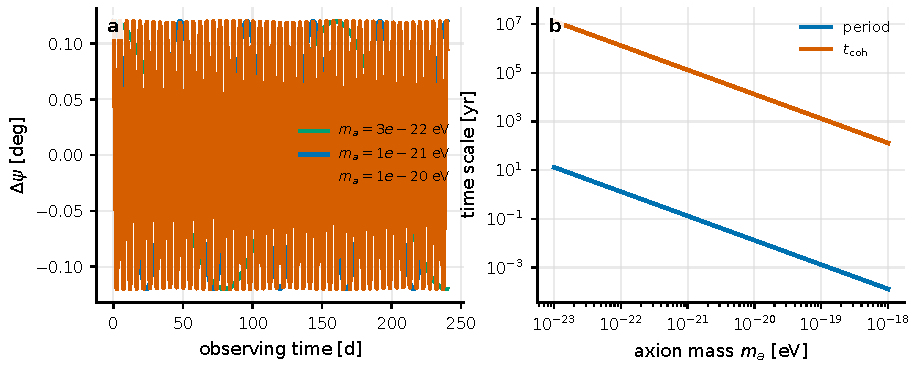
\includegraphics[width=0.94\linewidth]{figures/generated/chapter_15/ch15_axion_polarization_oscillation.pdf}
\caption{Ultralight dark matter turns polarization rotation into a time series. The left panel plots \(\Delta\psi(t)\) for three axion masses: the larger the mass, the faster the oscillation. The right panel converts the mass \(m_a\) into the period \(T_a\) and the coherence time \(t_{\rm coh}\sim T_a/v^2\) (taking \(v=10^{-3}c\)): the lighter the axion, the more slowly it swings, yet the longer it can keep the same phase.}
\label{fig:e22-oscillation}
\end{figure}


\section{How to measure such a small rotation: polarization-resolved intensity and coherence measurements}
\label{sec:e22-measure}

The target signal is often as small as \(10^{-3}\) radians or even smaller. This section makes clear: on what basis, and with what data structure, we catch it, and why ``catching a non-zero angle'' is often first a \emph{systematic-error} problem rather than a discovery.

\paragraph{The essence of polarization measurement: counting photons in a polarization basis}

Back to the foundation laid in Chapter~\ref{chap:e18}: the essence of polarization measurement is to split a beam of light into two (or several) orthogonal polarization channels and \emph{count photons separately}. Keeping accounts with the Stokes parameters (Stokes parameters) \(I,Q,U,V\), the linear-polarization information is all in \(Q\) and \(U\). The action of a polarization rotation \(\beta\) on \(Q,U\) is extremely clean: it multiplies the complex combination \(Q\pm iU\) by a phase factor,

\begin{equation}
  Q\pm iU \;\longrightarrow\; e^{\pm 2i\beta}\,(Q\pm iU).
  \label{eq:e22-qu-rotation}
\end{equation}
\begin{formulaexplain}
\(Q,U\): the linear-polarization Stokes parameters; \(\beta\): the overall polarization rotation angle. The \(2\beta\) (not \(\beta\)) in the exponent comes from the ``spin-2'' nature of linear polarization: polarization is an undirected double arrow, restored by a \(180^\circ\) rotation, so mathematically it appears as \(2\beta\).
\end{formulaexplain}

That \(2\) is crucial: it means a very small angular error is enough to let modes that should be clean contaminate each other. In spherical-harmonic (\(E/B\) mode) space, \eqref{eq:e22-qu-rotation} leaks \(E\) mode into \(B\) mode. If the source's own parity-odd spectrum is negligible, the parity-odd spectrum appearing after rotation is approximately

\begin{equation}
  C_\ell^{EB,\rm obs}=\tfrac12\sin(4\beta)\,(C_\ell^{EE}-C_\ell^{BB}),
  \qquad
  C_\ell^{TB,\rm obs}=\sin(2\beta)\,C_\ell^{TE}.
  \label{eq:e22-eb-tb}
\end{equation}
\begin{formulaexplain}
\(C_\ell^{EB},C_\ell^{TB}\): the parity-odd power spectra that emerge after rotation; \(\beta\): the rotation angle. If the source's intrinsic \(EB/TB\) is very small, a non-zero \(EB/TB\) becomes a probe of the rotation angle, but an error in the detector's angle calibration produces an almost identical shape.
\end{formulaexplain}

\paragraph{Cosmic birefringence: why it is first an angle-calibration problem}

The cosmic microwave background (CMB) is a tempting target for finding a ``global polarization rotation'': the last-scattering surface is extremely far, the sky area extremely large, and the statistics can be pushed very small. But it also forces a simple problem into the sharpest systematic-error problem. The universe itself rotating the polarization by \(\beta\) (cosmic birefringence, cosmic birefringence), and the detector's overall angle calibration being off by \(\alpha\), look almost identical in the CMB spectra: both produce the same-shaped \(EB\) through \eqref{eq:e22-eb-tb}. Plug in a number to feel the strength: at \(\beta=0.35^\circ\), \(\tfrac12\sin(4\beta)\simeq0.012\), that is, the \(EB\) leakage is only of order one percent of \(EE\!-\!BB\), the signal is already weak, and it is entangled with the calibration error. The Planck 2018 reanalysis pried the two partly apart with a clever trick: the CMB rotation \(\beta\) acts only on light from the last-scattering surface, while the Galactic-foreground polarization is right in front of us and is \emph{not} twisted by the cosmic rotation, and the two have different dependences on frequency and multipole, so one can fit \(\beta\) and the calibration angle \(\alpha\) simultaneously, giving \(\beta=0.35\pm0.14^\circ\) (\(68\%\) confidence). Subsequent WMAP+Planck and Planck PR4 analyses have repeatedly stressed that dust's own \(EB\), bandpass mismatch, \(I\to P\) leakage, cross-polarization response, and the choice of sky mask remain the main systematic errors weighing on this result \citep{2020PhRvL.125v1301M,2022NatRP...4..452K,2022PhRvD.106f3503E,2022PhRvL.128i1302D}. The original theoretical basis of cosmic birefringence can be traced to the discussion of pseudoscalar-field-induced optical rotation by Carroll, Field, Jackiw, and others \citep{1990PhRvD..41.1231C,1999PhRvL..83.1506L}.

\begin{figure}[tbp]
\centering
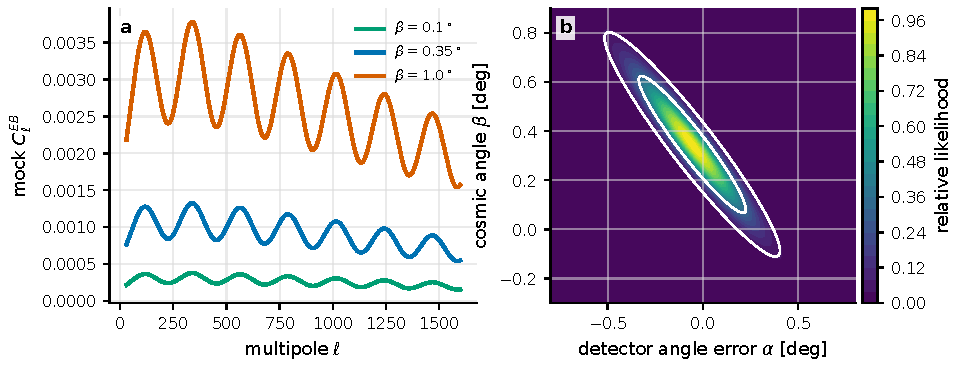
\includegraphics[width=0.94\linewidth]{figures/generated/chapter_15/ch15_cosmic_birefringence.pdf}
\caption{Cosmic birefringence simultaneously moves \(E/B\) mixing and the instrument angle calibration. The left panel uses toy \(EE\), \(BB\) spectra to demonstrate how the rotation angle \(\beta\) generates \(EB\) out of nothing. The right panel plots the degeneracy of the calibration angle \(\alpha\) and the cosmic rotation \(\beta\): looking only at the CMB, the two are nearly equivalent; only by relying on the frequency dependence of the foreground can the degeneracy be broken.}
\label{fig:e22-birefringence}
\end{figure}

\paragraph{Keep the measurement as an event table: do not average too early}

\Needspace{10\baselineskip}
More generally, the most robust approach is not to hurry to average the data into ``a map of a fixed polarization angle,'' but to keep it as a \emph{polarization event table} (following the event-table paradigm of Chapter~\ref{chap:e13}). Each photon event carries a time, frequency, direction, polarization channel, and weight:

\begin{equation}
  e_q=(t_q,\ \nu_q,\ \hat{\bm n}_q,\ p_q,\ w_q).
  \label{eq:e22-event}
\end{equation}
\begin{formulaexplain}
\(e_q\): the \(q\)-th polarization event; \(t_q,\nu_q,\hat{\bm n}_q\): the arrival time, frequency, celestial direction; \(p_q\): which polarization channel it falls into; \(w_q\): the quality weight. Keeping it as an event table lets one search for a ``common rotation'' in the time and frequency dimensions simultaneously, without first averaging away the phase information.
\end{formulaexplain}

If a small common oscillation \(\delta\psi\) is hidden in the polarization angle, the probability of falling into a given polarization channel is written as

\begin{equation}
  P\!\left(p_q\,\middle|\,t_q,\nu_q,\hat{\bm n}_q\right)
  = P_0\!\left[\,p_q\,\middle|\,\psi_{\rm src}
     +\psi_{\rm prop}(\nu_q,\hat{\bm n}_q)+\delta\psi(t_q,\hat{\bm n}_q)\,\right].
  \label{eq:e22-likelihood}
\end{equation}
\begin{formulaexplain}
\(\psi_{\rm src}\): the source's intrinsic polarization angle; \(\psi_{\rm prop}\): the propagation and instrument terms (including Faraday, dust, and the instrument Mueller matrix); \(\delta\psi\): the new-physics rotation to be tested. This likelihood splits the ``anomalous angle'' into several classes of \emph{mutually refutable} sources, put into the same fit together.
\end{formulaexplain}

The price is also frighteningly plain: if the off-diagonal terms of the instrument's Mueller matrix are calibrated only to \(10^{-3}\), while the rotation you seek is also \(10^{-3}\) radians, then the systematic error is already \emph{of the same order} as the signal: at which point a beautiful non-zero angle is most likely the instrument talking, not the universe. The optical polarization of isolated neutron stars, the X-ray polarization of magnetars, and the candidate signal of strong-field QED vacuum birefringence must all first have the source's geometry and propagation effects modeled clean before a polarization anomaly can possibly be interpreted as new physics \citep{2017MNRAS.465..492M}.


\section{Strong-field environments: compact objects as axion laboratories}
\label{sec:e22-strongfield}

The rotation channel relies on the axion field itself; the \emph{conversion} channel requires a strong magnetic field to turn the axion and photon directly into each other. Where are the strongest magnetic fields? Precisely the compact objects (neutron stars, magnetars) of Chapter~\ref{chap:e18} and the black holes of Chapter~\ref{chap:e19}. This section moves the polarization quantum channel into the strong-field environments of neutron stars, magnetars, and black holes, both computing the conversion probability and connecting to the boson cloud of superradiance.

\paragraph{Axion--photon conversion in a magnetic field}

In a transverse magnetic field \(B_\perp\), the axion mixes only with the photon polarization state parallel to \(B_\perp\). With weak mixing, a uniform magnetic field, and negligible absorption, the conversion probability is

\begin{equation}
  P_{a\to\gamma}\simeq\left(\frac{g_{a\gamma}B_\perp L}{2}\right)^2
  \mathrm{sinc}^2\!\left(\frac{qL}{2}\right),
  \qquad
  q\simeq\frac{|m_a^2-m_\gamma^2|}{2E}.
  \label{eq:e22-conversion}
\end{equation}
\begin{formulaexplain}
\(P_{a\to\gamma}\): the probability of an axion turning into a photon; \(B_\perp\): the transverse magnetic field; \(L\): the coherent path length; \(E\): the energy; \(m_\gamma\): the effective mass of the photon in the plasma; \(q\): the momentum mismatch of the axion and photon. The square out front gives the strength, and the \(\mathrm{sinc}^2\) factor governs coherence: once the phase mismatches, the accumulation is cut off.
\end{formulaexplain}

Please look at it side by side with the rotation formula \eqref{eq:e22-rotation}, and the contrast of the two kinds of ``distance dependence'' is clear at a glance. When \(qL\ll1\) (coherent), \(\mathrm{sinc}^2\to1\), and the probability grows as \(L^2\): \textbf{conversion accumulates along the way, the longer the travel the stronger}, which is exactly the opposite of ``rotation cares only about the two endpoints.'' But once \(qL\gtrsim\pi\), the conversion amplitudes of different path segments begin to cancel out of phase, \(\mathrm{sinc}^2\) decays rapidly, and no amount of extra length helps. This is the physics of the coherence length. Ground experiments use this formula to the hilt: CAST uses a decommissioned LHC dipole magnet (\(9\,\mathrm T\), \(9.26\,\mathrm m\)) to stare at the Sun, seeking X-rays converted from solar axions, and its 2013--2015 vacuum-pipe data gives \(g_{a\gamma}<0.66\times10^{-10}\,\mathrm{GeV^{-1}}\) (\(95\%\) confidence), applicable to the coherent low-mass region \(m_a\lesssim0.02\,\mathrm{eV}\) \citep{2017NatPh..13..584C}.

\begin{figure}[tbp]
\centering
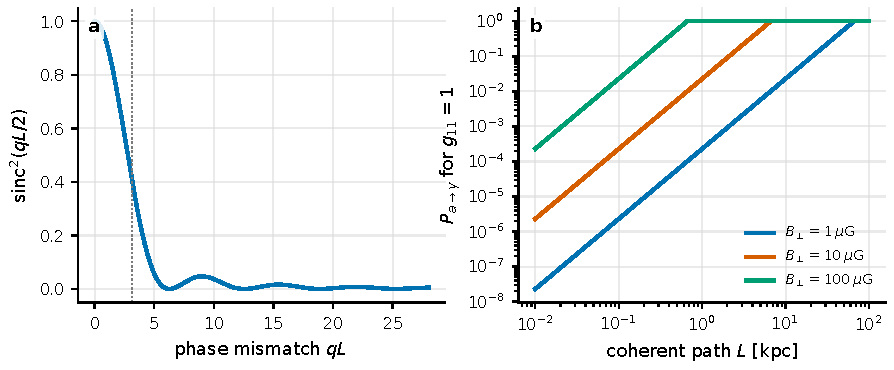
\includegraphics[width=0.94\linewidth]{figures/generated/chapter_15/ch15_axion_conversion.pdf}
\caption{Axion--photon conversion is determined jointly by intensity and phase. The left panel is the coherence factor \(\mathrm{sinc}^2(qL/2)\): as \(qL\) approaches \(\pi\), the conversion amplitudes of different parts of the path begin to cancel. The right panel gives the order of magnitude of the interstellar-scale coherence limit (taking \(g_{a\gamma}=10^{-11}\,\mathrm{GeV^{-1}}\)): in a \(\mu\mathrm G\) field over a kpc path, the single-segment conversion probability is usually far less than 1.}
\label{fig:e22-conversion}
\end{figure}

\paragraph{Magnetars and FRBs: extreme-magnetization polarization laboratories}

Neutron stars and magnetars push all of this to the limit: in Chapter~\ref{chap:e18} we already saw that the magnetic field at a magnetar surface approaches the critical field, and even the vacuum becomes a birefringent medium. This environment is a natural amplifier for axion conversion, but it also means that the intrinsic polarization structure and the propagation foreground are both extremely strong. Fast radio bursts (FRBs) give another class of extreme sample: FRB~121102 lies in a host galaxy at \(z=0.193\), and its \(4\text{--}8\,\mathrm{GHz}\) bursts show nearly \(100\%\) linear polarization, yet carry an absurdly high, time-varying Faraday rotation measure \(\mathrm{RM}_{\rm src}=1.46\times10^5\) and \(1.33\times10^5\,\mathrm{rad\,m^{-2}}\), with individual sub-structures as narrow as \(\lesssim30\,\mu\mathrm s\). If the host contributes \(\mathrm{DM_{host}}\sim70\text{--}270\,\mathrm{pc\,cm^{-3}}\), the inferred lower limit of the line-of-sight magnetic field already reaches order milligauss (mG), several hundred times the \(\sim5\,\mu\mathrm G\) of the ordinary Galactic interstellar medium \citep{2018Natur.553..182M}. This class of source is both a laboratory for extreme-magnetization plasma and the most cunning of impostors: a seemingly ``achromatic'' polarization variation must still first rule out depolarization caused by finite channel width, drift of \(\mathrm{RM}\) with time, and the selection effect of a plasma lens, before it is the axion's turn.

\begin{figure}[tbp]
\centering
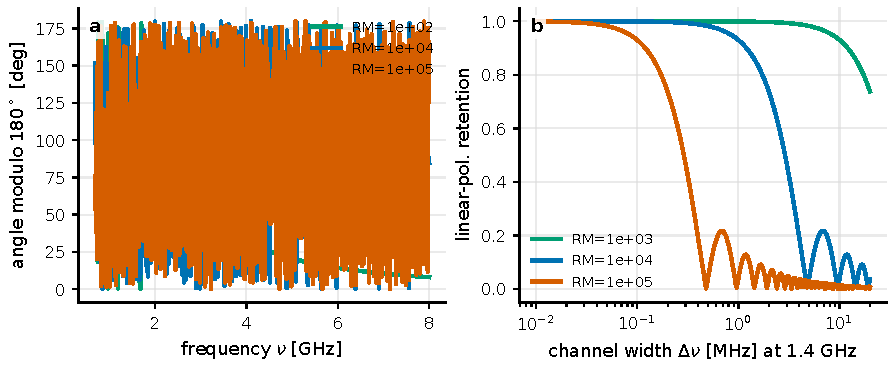
\includegraphics[width=0.94\linewidth]{figures/generated/chapter_15/ch15_frb_faraday_foreground.pdf}
\caption{The polarization foreground of an FRB can easily drown a weak rotation. The left panel plots the \(180^\circ\) wrapping of the polarization angle with frequency under different \(\mathrm{RM}\): \(\mathrm{RM}=10^5\,\mathrm{rad\,m^{-2}}\) varies extremely fast in the GHz band. The right panel is the linear-polarization retention fraction caused by finite channel width near \(1.4\,\mathrm{GHz}\): to measure such a high \(\mathrm{RM}\), one must use extremely narrow channels.}
\label{fig:e22-frb}
\end{figure}

\paragraph{Black hole superradiance: seeding a light boson field beside a spinning black hole}

A black hole ties a light boson field and the polarization picture into one. A boson wave orbiting a spinning (Kerr) black hole, provided its frequency is low enough to satisfy

\begin{equation}
  \omega<m\,\Omega_H,
  \label{eq:e22-superradiance}
\end{equation}
\begin{formulaexplain}
\(\omega\): the boson mode frequency; \(m\): the azimuthal quantum number (integer); \(\Omega_H\): the angular velocity of the Kerr black hole horizon. When this inequality is satisfied, the wave \emph{extracts} energy from the black hole's spin, grows exponentially, and piles up into a boson cloud orbiting the black hole.
\end{formulaexplain}

can extract energy from the black hole's spin, be amplified exponentially, and grow into a ``superradiant boson cloud'' (superradiant boson cloud). Whether the cloud can grow effectively depends on whether the axion Compton wavelength matches the black hole scale. Define a dimensionless ``gravitational fine-structure constant''

\begin{equation}
  \alpha_G=\frac{G M_\bullet m_a}{\hbar c},
  \label{eq:e22-alphaG}
\end{equation}
\begin{formulaexplain}
\(\alpha_G\): the ratio of the black hole gravitational radius to the axion Compton wavelength; \(M_\bullet\): the black hole mass. When \(\alpha_G\sim0.1\text{--}1\), the boson wave ``fits'' near the black hole, and superradiant growth is fastest.
\end{formulaexplain}

When \(\alpha_G\sim0.1\text{--}1\), the boson Compton wavelength matches the black hole scale, and the cloud grows most fiercely. Inverting \eqref{eq:e22-alphaG} maps the black hole mass to the axion mass it is most sensitive to:

\begin{equation}
  m_a\simeq 1.34\times10^{-10}\,\mathrm{eV}\;\alpha_G
  \left(\frac{M_\odot}{M_\bullet}\right).
  \label{eq:e22-bh-mass}
\end{equation}
\begin{formulaexplain}
Converting the black hole mass \(M_\bullet\) into the most-sensitive axion mass \(m_a\): the heavier the black hole, the lower the corresponding axion-mass window. So black holes of different mass probe different segments of the ultralight-mass spectrum.
\end{formulaexplain}

Take two real black holes. The Galactic-center Sgr~A\(^*\) (\(4.3\times10^6\,M_\odot\)) at \(\alpha_G=0.4\) corresponds to \(m_a\simeq1.2\times10^{-17}\,\mathrm{eV}\); M87\(^*\) (\(6.5\times10^9\,M_\odot\)) corresponds to \(8\times10^{-21}\,\mathrm{eV}\): the two black holes probe completely different mass segments. Here the polarization channel returns again: in EHT polarization imaging, an axion cloud makes the polarization angle on the ring swing together with the axion period, with Sgr~A\(^*\)'s period about \(100\text{--}1000\,\mathrm s\) and M87\(^*\)'s reaching several days. Whether this swing can be seen depends on the spatial resolution: if the different azimuths on the ring cannot be resolved, the swing is ``averaged'' out \citep{2015LNP...906.....B,2015CQGra..32m4001B,2017PhRvD..96c5019B,2020PhRvL.124f1102C,2022NatAs...6..592C}.

\begin{figure}[tbp]
\centering
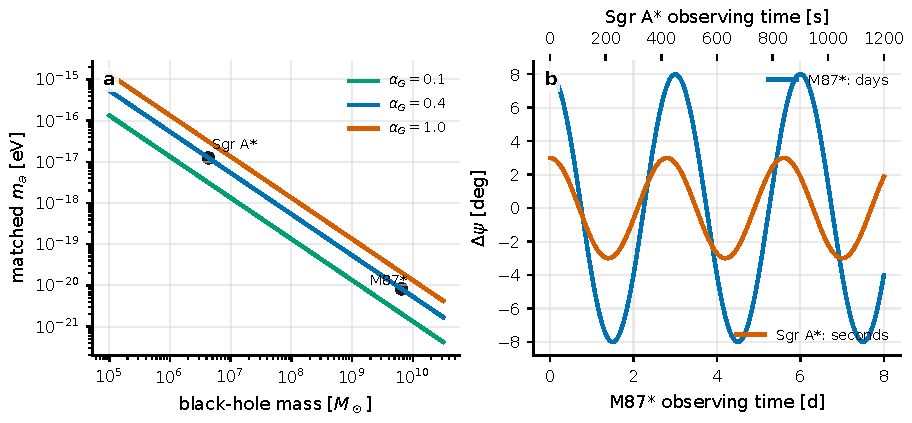
\includegraphics[width=0.94\linewidth]{figures/generated/chapter_15/ch15_black_hole_axion_cloud.pdf}
\caption{The black hole mass frames the mass window of the superradiant axion. The left panel uses \(\alpha_G=GM_\bullet m_a/\hbar c\) to mark the \(m_a\) corresponding to different black hole masses: Sgr~A\(^*\) and M87\(^*\) fall in different ultralight-mass segments. The right panel gives two typical timescales of the EHT polarization-angle oscillation: M87\(^*\) can be sampled on the day scale, while Sgr~A\(^*\) requires second-to-minute-scale polarization imaging.}
\label{fig:e22-bh}
\end{figure}


\section{Writing the anomaly as a refutable test}
\label{sec:e22-falsifiable}

By this point, all candidate signals share one iron law: \textbf{the anomaly itself is not the conclusion; the ``refutable structure'' of the anomaly is the conclusion}. This section gathers the tricks scattered above into a unified ledger.

\paragraph{One ledger: spread out and align the four classes of source}

The observables of a new-physics search are often more than one: polarization angle, arrival time, image position, magnification, possibly from different instruments, each carrying its own statistical and systematic error. Combining them into one data vector \(\bm d\), the model splits into four major blocks:

\begin{equation}
  \bm m(\bm\theta)=\bm m_{\rm src}+\bm m_{\rm prop}+\bm m_{\rm inst}+\bm m_{\rm new}(\bm\theta),
  \label{eq:e22-model-vector}
\end{equation}
\begin{formulaexplain}
\(\bm m\): the model prediction vector; the four terms are the source, propagation, instrument, and new physics. \(\bm\theta\): the new-physics parameters (\(g_{a\gamma}\), \(m_a\), \(\beta\), the subhalo mass function, etc.). This decomposition forces us to compare the anomaly with ordinary astrophysics, propagation foregrounds, and calibration errors in \emph{the same ledger}.
\end{formulaexplain}

In the Gaussian approximation, the objective function of the fit is

\begin{equation}
  -2\ln\mathcal L=\big[\bm d-\bm m(\bm\theta)\big]^{\mathsf T}
  \big(C_{\rm stat}+C_{\rm sys}\big)^{-1}
  \big[\bm d-\bm m(\bm\theta)\big]
  +\ln\det\big(C_{\rm stat}+C_{\rm sys}\big).
  \label{eq:e22-likelihood-gauss}
\end{equation}
\begin{formulaexplain}
\(\mathcal L\): the Gaussian likelihood; \(C_{\rm stat}\): the statistical covariance (photon noise, arrival-time error, image noise); \(C_{\rm sys}\): the systematic-error covariance (Mueller matrix, absolute polarization angle, Faraday foreground, dust \(EB\), lens macromodel, \ldots). The residual must be weighted by \emph{both} classes of error together; omit \(C_{\rm sys}\), and an isolated anomaly will be wrongly amplified.
\end{formulaexplain}

This expression makes mathematical the sentence this chapter keeps repeating: as long as \(C_{\rm sys}\) is not in the likelihood, any single anomalous point will be over-interpreted.

\paragraph{Five crowbars: making different signals betray one another}

Fortunately these signals have clear ways of distinguishing one another, and each corresponds to physics discussed earlier:

\begin{itemize}
\item \textbf{Wavelength dependence.} Faraday rotation goes as \(\lambda^2\) (Chapter~\ref{chap:e21}), axion rotation is approximately achromatic (\eqref{eq:e22-rotation}): measuring at several frequencies pries them apart.
\item \textbf{Temporal behavior.} Static cosmic birefringence gives an unchanging global angle (\eqref{eq:e22-eb-tb}), ultralight dark matter gives a breathing sinusoid (\eqref{eq:e22-osc-signal}): measuring over tens of days to years pries them apart.
\item \textbf{Black hole scaling.} The polarization oscillation of the superradiant cloud should be linked to the black hole mass, spin, azimuth on the ring, and observing time (\eqref{eq:e22-bh-mass}); an ordinary accretion flow does not so ``obey the black hole.''
\item \textbf{Path dependence.} Conversion accumulates along the way as \(L^2\) (\eqref{eq:e22-conversion}), while rotation cares only about the two endpoints: the distance responses of the two are exactly opposite.
\item \textbf{Cross-checks.} Sample statistics, blank fields or control sources, frequency inversion, temporal coherence, instrument recalibration: if any one of these fails, the ``discovery'' should be downgraded.
\end{itemize}

\paragraph{A parallel channel: how dark matter turns mass into an angular offset}

The polarization channel seeks ``the quantum effect of a field on photons''; there is also a parallel channel, seeking ``the effect of the dark-matter mass distribution on the light path'': gravitational lensing. It is likewise ``achromatic,'' likewise manifested not as ``seeing a clump of dark matter'' but as an image position, magnification, or arrival time deviating from the ordinary model. The existence of dark matter itself has multiple supports: galaxy-cluster collisions (such as the separation of the weak-lensing mass peak from the X-ray gas in the Bullet Cluster, indicating that the main mass is approximately collisionless), weak lensing, and dynamics \citep{2006ApJ...648L.109C,1993ApJ...404..441K}; and cold-dark-matter simulations predict that the Galactic halo is full of subhalos far below the visible satellite galaxies, becoming an important candidate explanation for strong-lensing anomalies \citep{1994ApJ...427L...1F,1999ApJ...524L..19M,2008Natur.454..735D}. The order of magnitude of subhalo lensing is given by the Einstein angle,

\begin{equation}
  \theta_E=\left(\frac{4GM}{c^2}\frac{D_{ls}}{D_lD_s}\right)^{1/2},
  \qquad
  \delta\theta\simeq\frac{\theta_E^2}{b},
  \label{eq:e22-lensing}
\end{equation}
\begin{formulaexplain}
\(\theta_E\): the subhalo Einstein angle, \(\propto M^{1/2}\); \(M\): the lens mass; \(D\): the combination of observer--lens--source distances; \(\delta\theta\): the astrometric offset of the image; \(b\): the angular distance of the image from the subhalo (\(b\gg\theta_E\)). The larger the mass and the closer to the image, the more marked the position perturbation; far away it decays as \(1/b\).
\end{formulaexplain}

The numbers set the resolution requirement very hard: in a galaxy strong lens with \(D_l\simeq1\,\mathrm{Gpc}\), \(D_s\simeq2\,\mathrm{Gpc}\), the \(\theta_E\) of a \(10^8\,M_\odot\) subhalo is a few tens of milliarcseconds (mas), and a \(10^6\,M_\odot\) one is only a few mas; while a \(10^6\,M_\odot\) subhalo at \(b=10\,\mathrm{mas}\) gives an astrometric offset of only order \(\mu\mathrm{as}\). The flux-ratio anomalies of strong lensing are sensitive to magnification perturbations: Mao and Schneider pointed out that low-mass substructure can explain the anomalies of some quadruple-image systems, Dalal and Kochanek used 7 radio lenses to measure a median substructure mass fraction \(f_{\rm sat}\simeq0.02\) (\(90\%\) range about \(0.006\text{--}0.07\)), and Vegetti, Hezaveh, and others used gravitational imaging and ALMA to push the detection of a single dark substructure to spatially resolved modeling \citep{1998MNRAS.295..587M,2002ApJ...572...25D,2010MNRAS.408.1969V,2016ApJ...823...37H}; Gaia and future astrometric surveys turn a subhalo transiting a background source into a time-domain signal, with the main limits coming from the scanning law, source density, and proper-motion covariance \citep{2024MNRAS.531..632M,2016PhRvD..94h3504C}. The ledger of this channel is entirely consistent with that of the polarization channel (\eqref{eq:e22-model-vector}): a dark subhalo should \emph{simultaneously} perturb the image position, magnification, and time delay, whereas stellar-surface structure varies mainly with source rotation, wavelength, and baseline direction. Put these distinctions into the same likelihood, and only then can an anomaly be upgraded to a discovery.

\begin{figure}[tbp]
\centering
\includegraphics[width=0.94\linewidth]{figures/generated/chapter_15/ch15_dark_matter_lensing.pdf}
\caption{The lensing signal of a dark-matter subhalo is limited by angular scale. The left panel gives the variation of the subhalo Einstein angle with mass for a typical Gpc geometry. The right panel converts \(\delta\theta\simeq\theta_E^2/b\) into an astrometric offset: a low-mass subhalo requires mas-level proximity and \(\mu\mathrm{as}\)-level systematic control to possibly be seen.}
\label{fig:e22-lensing}
\end{figure}

\paragraph{A time-domain corroboration: pulsar arrays}

The same ``common time term'' logic can also be used on pulsars. Pulsars have stable phases and repeating pulses, naturally suited to a time-domain array (pulsar timing array, PTA). The oscillation of the gravitational potential of ultralight scalar dark matter leaves a narrowband signal in the timing residuals: writing it as \(\Psi_c\cos(2m_at+\varphi)\), the simplified residual is

\begin{equation}
  R_\alpha(t)\simeq\frac{\Psi_c}{2\pi f}
  \Big[\sin(2\pi ft+\varphi_E)-\sin\!\big(2\pi f(t-D_\alpha/c)+\varphi_\alpha\big)\Big],
  \label{eq:e22-pta}
\end{equation}
\begin{formulaexplain}
\(R_\alpha\): the timing residual of the \(\alpha\)-th pulsar; \(\Psi_c\): the potential-oscillation amplitude; \(f\simeq m_a/\pi\): the narrowband frequency; \(D_\alpha\): the pulsar distance. The first term is the ``Earth term'' shared by all pulsars, and the second is each star's own ``pulsar term.''
\end{formulaexplain}

\(m_a\sim10^{-23}\,\mathrm{eV}\) corresponds to \(f\sim10^{-8}\,\mathrm{Hz}\), falling right in the PTA window of \(10^{-9}\text{--}10^{-7}\,\mathrm{Hz}\). Porayko and Postnov analyzed old NANOGrav data and gave an upper limit \(\Psi_c<1.14\times10^{-15}\) (\(95\%\) confidence) \citep{2014PhRvD..90f2008P}. The inter-pulsar correlation of this scalar template hardly depends on the angle between two stars, and is therefore different from the famous Hellings--Downs angular-correlation curve of a stochastic gravitational-wave background: this is itself another crowbar. If a ``pulsar polarization array'' is done in the future, one must likewise separate out the common Earth term, the intrinsic magnetospheric polarization, the interstellar Faraday rotation, pulse-profile variations, and receiver polarization leakage one by one.

\begin{figure}[tbp]
\centering
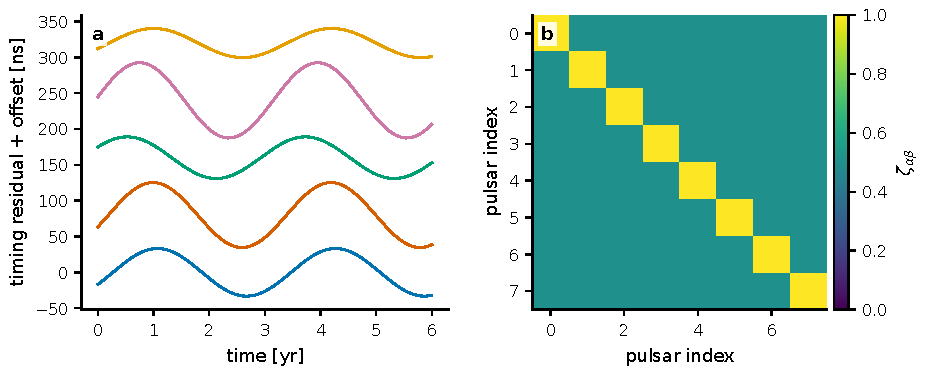
\includegraphics[width=0.94\linewidth]{figures/generated/chapter_15/ch15_pulsar_array_correlation.pdf}
\caption{The common narrowband signal in a pulsar array. The left panel is a common Earth term superimposed on each star's own pulsar term (the curves are artificially offset for viewing). The right panel gives the simplified correlation matrix of the scalar-potential-oscillation model \(\zeta_{\alpha\beta}=(1+\delta_{\alpha\beta})/2\), which differs from the angular correlation of a stochastic tensor gravitational-wave background.}
\label{fig:e22-pta}
\end{figure}


\section{Chapter Summary}
\label{sec:e22-summary}

\begin{itemize}
\item \textbf{One coupling, two observables.} The minimal \(a\,\bm E\cdot\bm B\) coupling (\eqref{eq:e22-lagrangian}) opens two quantum channels simultaneously: the axion background \emph{twists} the plane of linear polarization, and in a strong magnetic field the axion and photon \emph{convert} into each other. Both measure polarization, yet the physics is complementary.
\item \textbf{The rotation angle cares only about the two endpoints, and is achromatic.} The phase difference is the integral of a total differential along the path, leaving only the endpoint difference (\eqref{eq:e22-phase-diff}), and the rotation angle is half of it (\eqref{eq:e22-rotation}), and it \emph{contains no wavelength}: this is the first crowbar that separates it from Faraday rotation (\(\propto\lambda^2\)).
\item \textbf{Dark matter makes polarization breathe.} If the axion is ultralight dark matter, the field oscillates with time (\eqref{eq:e22-dm-field}), and the rotation angle becomes a quasi-monochromatic sinusoid (\eqref{eq:e22-osc-signal}); the period is tens of days and the coherence time can reach \(10^5\) years (\eqref{eq:e22-timescales}): the search must look for a common swing over a long time baseline, not measure only once.
\item \textbf{The essence of measurement is counting photons in a polarization basis.} The \(2\beta\) of Stokes rotation (\eqref{eq:e22-qu-rotation}) leaks \(E\) into \(B\) (\eqref{eq:e22-eb-tb}); CMB birefringence is first a degeneracy problem between \(\beta\) and the calibration angle \(\alpha\), and the result \(\beta=0.35\pm0.14^\circ\) relies entirely on the foreground frequency dependence to break the degeneracy. Keeping the data as an event table (\eqref{eq:e22-event}, \eqref{eq:e22-likelihood}) avoids averaging away the signal too early.
\item \textbf{Conversion accumulates along the way, and compact objects are amplifiers.} \(P_{a\to\gamma}\propto(g_{a\gamma}B_\perp L)^2\,\mathrm{sinc}^2(qL/2)\) (\eqref{eq:e22-conversion}) grows as \(L^2\) in the coherent region; the extreme magnetization of magnetars and FRBs and the black hole superradiant boson cloud (\eqref{eq:e22-superradiance}--\eqref{eq:e22-bh-mass}) move the polarization channel into strong fields, at the price of an equally fierce intrinsic structure and foreground.
\item \textbf{An anomaly must be written as a refutable ledger.} Split the source, propagation, instrument, and new physics apart (\eqref{eq:e22-model-vector}), and weight with \(C_{\rm stat}+C_{\rm sys}\) together (\eqref{eq:e22-likelihood-gauss}); rely on the five crowbars of wavelength, time, black hole scaling, path dependence, and cross-checks to make the signals betray one another. Lensing (\eqref{eq:e22-lensing}) and PTA (\eqref{eq:e22-pta}) are parallel channels of the same logic.
\end{itemize}

\noindent\textbf{Questions to Ponder.}
(1) Why does the field value ``in the middle of the path'' not appear at all in the axion rotation formula \eqref{eq:e22-rotation}, while the conversion formula \eqref{eq:e22-conversion} is extremely sensitive to the path length \(L\)? How can this difference in the two kinds of ``distance dependence'' help you separate them in real data?
(2) If a telescope's polarization-angle calibration error is \(0.5^\circ\) and the cosmic birefringence you seek is \(0.35^\circ\), do you have any way, using \emph{only} this one instrument, to separate the two? Why can ``using the frequency dependence of the foreground'' come to the rescue?
(3) Sgr~A\(^*\) and M87\(^*\) probe completely different axion-mass segments (\eqref{eq:e22-bh-mass}). Suppose one day you see the polarization angle on M87\(^*\)'s ring oscillating with a period of several days; would you first suspect it is an axion cloud, or first suspect the accretion flow itself? Which cross-checks would you need before you dare to upgrade it to a ``discovery''?

\chapter{Quantum Problems in Cosmology}
\label{chap:e23}

\begin{chapteropening}
In the previous chapters we pointed our telescopes at a star, an accretion disk, a burst: sources you can go back and look at again another night, whose bandwidth you can tune, whose experiment you can redo. The object of this chapter is one and only one, and it happens only once: \textbf{the entire universe}. It is an optical experiment that took place long ago and cannot be restarted; we merely set up our detector very late, to read a plate it left on the sky. This plate is the cosmic microwave background (cosmic microwave background, CMB): an almost perfect blackbody microwave sky, overlaid with temperature patterns of order \(10^{-5}\) and even fainter polarization structure.

This chapter answers three progressively deeper questions. First, \textbf{where do these patterns come from}? We will see that their seeds are the \emph{quantum} vacuum fluctuations amplified during inflation, together with one crucial turn: how these quantum fluctuations ``become,'' through decoherence, density perturbations describable by a classical random field. Second, \textbf{what does a beam of light experience crossing billions of light-years}? Its polarization may be quietly rotated by a small angle, and its arrival time may be pulled apart by the medium and by deeper physics. Third, \textbf{can we use a cosmologically long baseline to weigh the most fundamental physics}: Lorentz invariance, the upper limit on the photon mass? Bringing abstract cosmology, step by step, back down to the coherence, polarization, and photon arrival times familiar from this book.
\end{chapteropening}

\section{The universe as a one-shot optical experiment}
\label{sec:e23-lightfield}

Let us set the scene. When people talk about the CMB they open with ``inflationary quantum fluctuations,'' but the observational entry point is in fact very plain: the telescope first sees an almost perfect blackbody microwave sky, and then, on top of this mean background, measures a thin layer of angular fluctuations. So this section first weighs the CMB as a \emph{light field}, and then retreats all the way back to the early quantum modes that produced these patterns.

The mean CMB is a blackbody of temperature \(T_0=2.7255\pm0.0006\,{\rm K}\). Chapter~\ref{chap:e05} quantized the light field and wrote down the Planck blackbody formula, and Chapter~\ref{chap:e06} specifically discussed the thermal state (thermal state): in a thermal light field the mean photon occupation number of each frequency mode is given by the Bose distribution, and the specific intensity by the Planck formula:
\begin{equation}
  n_\nu=\frac{1}{\exp(h\nu/k_{\rm B}T_0)-1},
  \qquad
  I_\nu=\frac{2h\nu^3}{c^2}\,n_\nu .
  \label{eq:e23-planck-spectrum}
\end{equation}
\begin{formulaexplain}
\(n_\nu\) is the mean photon number in a single frequency mode, and \(I_\nu\) is the blackbody specific intensity. At the low-frequency end \(n_\nu\) is large and the field is close to classical thermal light; at the high-frequency end \(n_\nu<1\), and a single mode often has less than one photon.
\end{formulaexplain}
Symbol by symbol: \(\nu\) is in Hz, \(h\) is the Planck constant, \(k_{\rm B}\) is the Boltzmann constant, and \(I_\nu\) is in \({\rm erg\,s^{-1}\,cm^{-2}\,Hz^{-1}\,sr^{-1}}\) (the CMB literature often converts to \({\rm MJy\,sr^{-1}}\)). Plug in two real frequencies to get a feel: at \(30\,{\rm GHz}\), \(h\nu/k_{\rm B}T_0\simeq0.53\), so \(n_\nu\simeq1/(e^{0.53}-1)\simeq1.4\), and the low-frequency channel is still a near-classical thermal field; at \(150\,{\rm GHz}\), the exponent grows, \(n_\nu\simeq0.07\), and the single-mode occupation is already less than 1. The blackbody intensity peak falls near \(160\,{\rm GHz}\): this is precisely the physical reason the Planck high-frequency instrument and many ground experiments choose channels at \(90/150/220\,{\rm GHz}\). FIRAS measured this mean spectrum extremely close to an ideal blackbody, so modern cosmology simply treats the mean spectrum as a \emph{known background} and puts all the information into the angular fluctuations and polarization on top of it \citep{1994ApJ...420..439M,1996ApJ...473..576F,2009ApJ...707..916F}.

Expanding the fluctuations on the sky into spherical harmonics (spherical harmonics) is like expanding a stretch of sound into different pitches:
\begin{equation}
  T(\hat{\bm n})=T_0\,[1+\Theta(\hat{\bm n})],
  \qquad
  \Theta(\hat{\bm n})=\sum_{\ell m}a^{T}_{\ell m}\,Y_{\ell m}(\hat{\bm n}).
  \label{eq:e23-temperature-expansion}
\end{equation}
\begin{formulaexplain}
\(\Theta\) is the dimensionless temperature fluctuation, \(a^{T}_{\ell m}\) are the spherical-harmonic coefficients, and \(Y_{\ell m}\) are the spherical-harmonic functions. This expression breaks a sky map into layers of angular scale: \(\ell\) sets the scale, and \(m\) governs the azimuthal pattern at the same scale.
\end{formulaexplain}
Here \(\hat{\bm n}\) is the sky direction (a unit vector), and the multipole \(\ell\) is approximately related to angular scale by \(\theta\simeq180^\circ/\ell\): \(\ell\simeq2\) is a pattern as large as half the sky, \(\ell\simeq200\) is about one degree, and \(\ell\simeq2000\) is only a few arcminutes. The differential microwave radiometer of COBE first saw \(\Delta T/T\sim10^{-5}\) structure on an all-sky map, and Planck decomposed it all the way to \(\ell\sim2500\). For an isotropic Gaussian sky, squaring and averaging all the \(m\) at the same \(\ell\) gives the angular power spectrum (angular power spectrum):
\begin{equation}
  \widehat C^{TT}_\ell=\frac{1}{2\ell+1}\sum_{m=-\ell}^{\ell}\bigl|a^{T}_{\ell m}\bigr|^2,
  \qquad
  D^{TT}_\ell=\frac{\ell(\ell+1)}{2\pi}\,C^{TT}_\ell .
  \label{eq:e23-cl-estimator}
\end{equation}
\begin{formulaexplain}
\(\widehat C^{TT}_\ell\) is the temperature angular-power-spectrum estimator, from the average of all \(2\ell+1\) modes \(m\) at one \(\ell\); \(D_\ell\) is the rescaled form commonly used for plotting. This average is the core compression of the CMB two-point statistics.
\end{formulaexplain}
If \(a_{\ell m}\) is in units of \(\mu{\rm K}\), then \(C_\ell\) and \(D_\ell\) are in \(\mu{\rm K}^2\). The first acoustic peak of \(D^{TT}_\ell\) is at \(\ell\simeq220\), with a peak height of about \(5\times10^3\,\mu{\rm K}^2\). These peaks are not random; they come from the \emph{acoustic oscillations} of the photon--baryon fluid before recombination (recombination): the baryon density changes the height of the compression peaks, the dark-matter density changes the decay of the gravitational potential, and the angular diameter distance projects the physical acoustic scale onto an angular scale on the sky. Planck fits these peaks with a six-parameter flat \(\Lambda{\rm CDM}\) model, giving typical precision such as \(\Omega_bh^2\simeq0.0224\), \(\Omega_ch^2\simeq0.120\), \(n_s\simeq0.965\), \(H_0\simeq67.4\,{\rm km\,s^{-1}\,Mpc^{-1}}\) \citep{1992ApJ...396L...1S,1996ApJ...469..437S,2020A&A...641A...5P,2020A&A...641A...6P}. Here \(\Omega_x\) is the dimensionless density parameter of the \(x\)-th component (the ratio of that component's density to the critical density), \(h\equiv H_0/(100\,{\rm km\,s^{-1}\,Mpc^{-1}})\) is the reduced Hubble constant, and the reason for writing the combination \(\Omega h^2\) is that what the CMB directly constrains is the physical density, independent of the value of \(H_0\): these are all outputs of the six-parameter fit, and if one wishes to examine the origin of the notation in detail, consult any cosmology textbook; this book merely uses them as known numbers.

Here is a ``happens only once'' cosmology-specific limitation. Even if the instrument were perfect and noiseless, at each \(\ell\) the sky gives you only \(2\ell+1\) modes \(m\), that is all the sample there is, and the variance cannot be dodged. This is called cosmic variance (cosmic variance):
\begin{equation}
  \frac{\sigma(C_\ell)}{C_\ell}=\sqrt{\frac{2}{(2\ell+1)\,f_{\rm sky}}} .
  \label{eq:e23-cosmic-variance}
\end{equation}
\begin{formulaexplain}
\(\sigma(C_\ell)/C_\ell\) is the relative error from sample variance, and \(f_{\rm sky}\) is the effective sky fraction. Low \(\ell\) has few usable modes, so large angular scales inherently carry a layer of statistical uncertainty that cannot be removed by sensitivity.
\end{formulaexplain}
\(f_{\rm sky}\) is the fraction of the sky used (the Galactic plane and strong foregrounds must be masked, so usually \(f_{\rm sky}<1\)). Plug in numbers: the relative error at all-sky \(\ell=2\) is about \(\sqrt{2/5}\simeq63\%\), dropping to about \(7\%\) at \(\ell=200\), and only about \(2.2\%\) at \(\ell=2000\). This is why phenomena such as ``low-\(\ell\) anomalies'' and ``a low quadrupole'' must be judged within the covariance of a finite number of modes, and not merely because they look conspicuous on the plot. This is of one spirit with the error budget of Chapter~\ref{chap:e15}: first ask ``how much independent information do I actually have.''

The polarization map has two more Stokes parameters, \(Q\) and \(U\), than the temperature map. They are not scalars, but \emph{spin-2} (spin-2) quantities that rotate with the coordinates, so they must be expanded in spin-weighted spherical harmonics and then linearly combined into two modes of definite parity:
\begin{equation}
  (Q\pm iU)(\hat{\bm n})=\sum_{\ell m}a_{\pm2,\ell m}\,{}_{\pm2}Y_{\ell m}(\hat{\bm n}),
  \quad
  a^{E}_{\ell m}=-\tfrac12(a_{2,\ell m}+a_{-2,\ell m}),
  \quad
  a^{B}_{\ell m}=\tfrac{i}{2}(a_{2,\ell m}-a_{-2,\ell m}).
  \label{eq:e23-eb-definition}
\end{equation}
\begin{formulaexplain}
\(Q\pm iU\) are the spin-\(\pm2\) polarization fields, \({}_{\pm2}Y_{\ell m}\) are the spin-weighted spherical harmonics, and \(a^{E/B}_{\ell m}\) are the E/B-mode coefficients. This combination translates the pointwise polarization direction into two classes of all-sky patterns.
\end{formulaexplain}
The key physics lies in parity: the \(E\) mode behaves like a scalar under a mirror transformation (the polarization directions form a radial or concentric pattern around hot and cold spots), while the \(B\) mode behaves like a pseudoscalar (with a vortical feel). Linear-order scalar density fluctuations produce mainly \(T\) and \(E\), and do \emph{not} directly produce primordial \(B\). Only a few things can produce \(B\): primordial tensor perturbations (gravitational waves), weak gravitational lensing, an overall rotation of the polarization angle, and Galactic dust and synchrotron foregrounds. Keep this in mind: \textbf{\(B\) modes are rare guests}, and whoever can cleanly create them carries the deepest cosmological information. This thread will be pulled twice later in this chapter: once toward primordial gravitational waves, once toward polarization birefringence. These two light-field skeleton diagrams are shown in Figures~\ref{fig:e23-blackbody} and \ref{fig:e23-power}.

\begin{figure}[tbp]
\centering
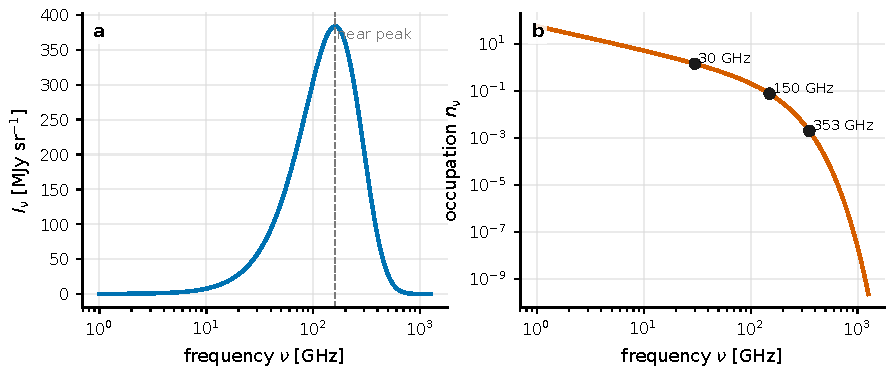
\includegraphics[width=0.9\linewidth]{figures/generated/chapter_16/ch16_cmb_blackbody.pdf}
\caption{The mean light field of the CMB is determined jointly by the blackbody spectrum and the mode occupation number. The left panel writes the Planck spectrum at \(T_0=2.7255\,{\rm K}\) in \({\rm MJy\,sr^{-1}}\), peaking near \(160\,{\rm GHz}\); the right panel is the single-mode mean photon number \(n_\nu\) of the same blackbody at different frequencies, with the low-frequency channels having higher occupation and the high-frequency channels gradually entering \(n_\nu<1\).}
\label{fig:e23-blackbody}
\end{figure}

\begin{figure}[tbp]
\centering
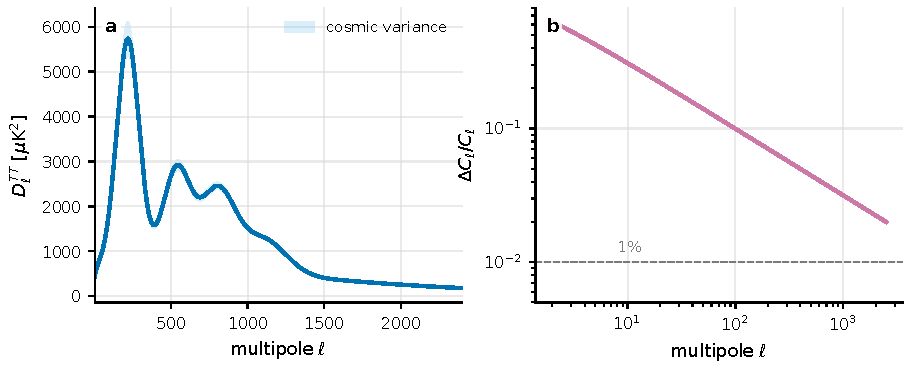
\includegraphics[width=0.9\linewidth]{figures/generated/chapter_16/ch16_cmb_power_spectrum.pdf}
\caption{The angular power spectrum compresses the sky fluctuations into multipole space. The left panel is \(D_\ell^{TT}\) with acoustic peaks and a damping tail, with the shading showing the order of magnitude of all-sky cosmic variance; the right panel plots \(\sqrt{2/(2\ell+1)}\) alone, showing that the error at large angular scales is set by the number of usable modes on the sky, a variance no amount of telescope sensitivity can remove.}
\label{fig:e23-power}
\end{figure}

\section{Inflation: amplifying vacuum fluctuations into density perturbations}
\label{sec:e23-inflation}

The \(C_\ell\) of the previous section is a statistic on the sky; what inflation (inflation) theory must explain is why these statistics are \emph{nearly Gaussian}, \emph{nearly scale-invariant}, and why the phases of the acoustic peaks are fixed (not a jumble of random-phase noise). Here we cannot treat the CMB as a laboratory beam that can be repeatedly prepared, but must regard every field mode in the early universe as the familiar quantum harmonic oscillator of Chapter~\ref{chap:e04}, only its frequency varies with cosmic expansion.

For the scalar curvature perturbation \(\mathcal R\), one defines a Mukhanov--Sasaki variable \(v\) that ``packages'' the background evolution in:
\begin{equation}
  v(\bm x,\eta)=z(\eta)\,\mathcal R(\bm x,\eta),
  \qquad
  z=\frac{a\,\dot\phi}{H} .
  \label{eq:e23-ms-variable}
\end{equation}
\begin{formulaexplain}
\(v\) is the Mukhanov--Sasaki variable, \(\mathcal R\) is the curvature perturbation we ultimately care about, and \(z=a\dot\phi/H\) packs the background evolution of inflation into a single coefficient. Writing the equations with \(v\), each Fourier mode becomes a quantum harmonic oscillator with a time-varying frequency.
\end{formulaexplain}
Symbol by symbol: \(\eta\) is conformal time (conformal time, satisfying \({\rm d}\eta={\rm d}t/a\)), \(a\) is the scale factor (dimensionless, set to 1 today), \(\phi\) is the background scalar field driving inflation, \(H=\dot a/a\) is the Hubble rate (in \({\rm s^{-1}}\)), and the dot denotes a derivative with respect to cosmic time. Expanding the second-order action for each Fourier mode \(v_k\) yields an equation of motion of extremely clean form:
\begin{equation}
  v_k''+\Bigl(k^2-\frac{z''}{z}\Bigr)v_k=0 .
  \label{eq:e23-ms-equation}
\end{equation}
\begin{formulaexplain}
\(v_k\) is the mode function of comoving wavenumber \(k\), and the prime is a derivative with respect to conformal time \(\eta\). The \(k^2-z''/z\) in the brackets is the squared effective frequency of this ``time-varying oscillator,'' and the flip of its sign is precisely all the magic of inflation.
\end{formulaexplain}
\(k\) is the comoving wavenumber (comoving wavenumber, in \({\rm Mpc^{-1}}\)). The two limits of this equation determine everything; let us read them out one by one:

\emph{Sub-horizon} (\(k\gg aH\)): \(z''/z\) is negligible compared with \(k^2\), and the equation degenerates into \(v_k''+k^2v_k=0\), an ordinary simple harmonic oscillator. Taking its quantum vacuum (the Bunch--Davies vacuum), the normalized mode function is
\[
  v_k(\eta)\simeq\frac{e^{-ik\eta}}{\sqrt{2k}} .
\]
This is precisely the vacuum fluctuation of ``the lowest energy state still jittering'' that this book has discussed from the very beginning, only occurring on every short-wave mode of the early universe.

\emph{Horizon exit} (\(k\simeq aH\), and thereafter \(k\ll aH\)): expansion pushes \(z''/z\) up so that it dominates the equation. Now the growing solution no longer oscillates but is \emph{frozen}, the decaying solution shrinks rapidly, and \(\mathcal R_k=v_k/z\) tends to a nearly constant. ``Frozen'' does not mean the mode stops evolving, but that one direction in phase space is strongly narrowed, leaving in the end only a single random amplitude to govern the later density perturbations \citep{1988JETP...67.1297M,1990PhRvD..42.3413G,1996CQGra..13..377P}.

Writing this frozen two-point statistic as the dimensionless primordial curvature power spectrum:
\begin{equation}
  \langle\mathcal R_{\bm k}\mathcal R_{\bm k'}\rangle
  =(2\pi)^3\delta^{(3)}(\bm k+\bm k')\,\frac{2\pi^2}{k^3}\,\mathcal P_{\mathcal R}(k),
  \qquad
  \mathcal P_{\mathcal R}(k)=A_s\Bigl(\frac{k}{k_*}\Bigr)^{n_s-1} .
  \label{eq:e23-primordial-spectrum}
\end{equation}
\begin{formulaexplain}
\(\mathcal P_{\mathcal R}\) is the dimensionless primordial curvature power spectrum, \(A_s\) is the amplitude, \(n_s\) is the spectral index (spectral index), and \(k_*\) is the reference wavenumber (pivot). It condenses the early quantum fluctuations' two-point statistics into the two most central numbers of today's CMB fits.
\end{formulaexplain}
Planck commonly takes the pivot \(k_*=0.05\,{\rm Mpc^{-1}}\), giving \(\ln(10^{10}A_s)\simeq3.04\), i.e.\ \(A_s\simeq2.1\times10^{-9}\). The spectral index \(n_s=1\) is exact scale invariance; the measured \(n_s\simeq0.965\) shows a slight ``red tilt,'' the long waves slightly stronger than the short waves, precisely the small deviation expected from slow-roll inflation. Keep this order-of-magnitude chain firmly in mind: a primordial curvature power of \(10^{-9}\), passed through the radiation transfer function, the acoustic oscillations, the finite thickness of the recombination surface, and later lensing smoothing, is projected into the patterns of \(\Delta T/T\sim10^{-5}\) on the sky today \citep{2020A&A...641A...6P,2020A&A...641A..10P}.

Now let us translate it into the quantum-optics language of this book. The time-varying background of inflation evolves the pair of modes \(\bm k\) and \(-\bm k\) from the vacuum into a \emph{two-mode squeezed state} (two-mode squeezed state), as was said when introducing squeezed states in Chapter~\ref{chap:e06}, squeezing means ``amplifying the fluctuations of a pair of modes in pairs, while maintaining a fixed phase relation'':
\begin{equation}
  |\psi\rangle=\prod_{\bm k}\exp\!\Bigl[\,r_k e^{-2i\varphi_k}\,\hat a_{\bm k}\hat a_{-\bm k}
  -r_k e^{2i\varphi_k}\,\hat a^\dagger_{\bm k}\hat a^\dagger_{-\bm k}\Bigr]\,|0\rangle .
  \label{eq:e23-squeezed-state}
\end{equation}
\begin{formulaexplain}
\(|\psi\rangle\) is the two-mode squeezed state of the pair \(\bm k\) and \(-\bm k\), \(r_k\) is the squeezing strength, \(\varphi_k\) is the squeezing angle, and \(\hat a,\hat a^\dagger\) are the annihilation and creation operators. Inflation amplifies the vacuum fluctuations in pairs and locks their phases.
\end{formulaexplain}
The mean occupation number of each pair of modes is \(N_k=\sinh^2 r_k\). After \(50\text{--}60\) e-folds (the logarithm of the amount of expansion), \(r_k\) is very large, and \(N_k\) grows exponentially. A reminder: the ``occupation number'' here refers to the number of quantum excitations of the early \emph{field modes}, which is not the same thing as the number of CMB photons the telescope actually counts today. In phase space, squeezing stretches the Wigner function into a very thin, elongated ellipse: one direction is stretched long (the one that later serves as the classical random amplitude), and the other is squeezed very narrow. It is precisely this squeezed-dead direction that locks the fixed phase, thereby arranging a regular string of acoustic peaks in the \(TT\), \(TE\), \(EE\) spectra, rather than random noise (Figure~\ref{fig:e23-squeezed}) \citep{1990PhRvD..42.3413G,1996CQGra..13..377P,2006CQGra..23.2317P}.

\begin{figure}[tbp]
\centering
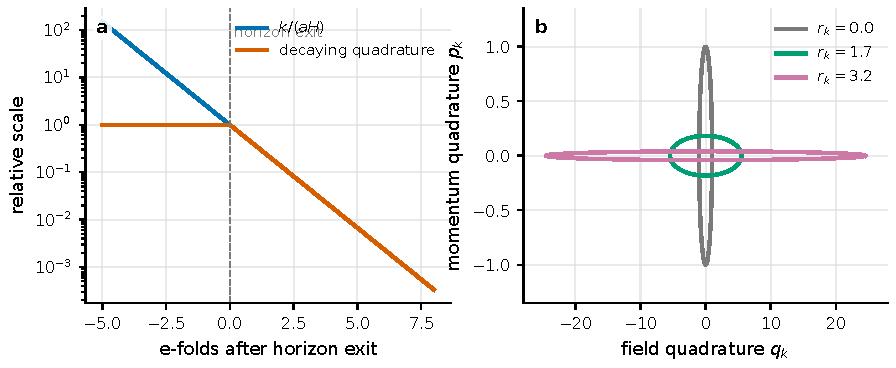
\includegraphics[width=0.9\linewidth]{figures/generated/chapter_16/ch16_squeezed_modes.pdf}
\caption{Mode amplification during inflation can be viewed as two-mode squeezing. The left panel shows \(k/(aH)\) falling exponentially after horizon exit, with the decaying direction squeezed narrow; the right panel plots the phase-space ellipse, with one direction stretched long and the other squeezed dead as \(r_k\) grows, and what is observed is the long axis, which later behaves as the classical random amplitude.}
\label{fig:e23-squeezed}
\end{figure}

\section{Decoherence: how quantum fluctuations ``become'' classical density perturbations}
\label{sec:e23-decoherence}

The previous section left an unease: if each mode is still a pure quantum squeezed state, it is a quantum superposition: how can it be used directly as a classical density fluctuation to compute how galaxies grow? The answer is decoherence (decoherence). This is also the first true ``quantum problem'' of this chapter: \textbf{why does an amplified quantum state behave observationally like a classical random field}?

First a picture. The ``quantumness'' of a quantum state is hidden in the \emph{off-diagonal terms} of its density matrix: the evidence that different amplitude branches can still interfere with each other. But these inflationary modes are not isolated: they are entangled with a great mass of unobserved degrees of freedom (unobserved short-wave modes, tensor--scalar interactions, degrees of freedom of the pre-recombination plasma, the lensing potential, and even the foreground and instrument modes marginalized away in data analysis). Once these environments are summed and integrated out, the off-diagonal terms of the reduced density matrix of the observed variable \(q_k\) are rapidly flattened by a Gaussian factor:
\begin{equation}
  \rho_{\rm red}(q,q')=\rho_0(q,q')\,\exp\!\bigl[-\Gamma_k\,(q-q')^2\bigr] .
  \label{eq:e23-decoherence-density}
\end{equation}
\begin{formulaexplain}
\(\rho_{\rm red}\) is the reduced density matrix of the observed variable \(q_k\), \(\rho_0\) is the undecohered form, and \(\Gamma_k\) measures the strength with which the environment flattens the off-diagonal terms. When the coherence term for \(q\ne q'\) is squeezed dead, the power spectrum can be computed with a classical random field.
\end{formulaexplain}
Reading this expression word by word: \(q,q'\) are two different values of the same observed variable, and a larger \((q-q')\) means the two branches are farther apart; the exponential factor \(\exp[-\Gamma_k(q-q')^2]\) is a bell-shaped ``valve'' that almost completely shuts off the interference between branches that are farther apart. The dimension of \(\Gamma_k\) depends on how \(q_k\) is normalized, but the physical criterion is crisp: as long as \(\Gamma_k(\Delta q)^2\gg1\), the different amplitude branches will never again interfere, and the two-point function, the angular power spectrum \(C_\ell\), the angular bispectrum (bispectrum), and lensing reconstruction can all be computed honestly with a classical random field. For inflationary modes, the stronger the squeezing and the deeper the entanglement, the larger \(\Gamma_k\), and this condition is enormously satisfied. This is precisely the exact meaning of the sentence ``quantum fluctuations become classical density perturbations.''

To prevent misunderstanding, a word about the boundary. Decoherence makes the \emph{statistics} classical, but it does not answer for us ``which branch was actually realized'': the ``measurement problem'' of the early universe remains conceptually debated. However, for the quantities we can measure (\(C_\ell\), lensing reconstruction, higher-order correlations), the residual coherent phase information is too little, long since insufficient to support a laboratory-style Bell test, and unable to treat the CMB as a repeatedly preparable non-classical state to manipulate \citep{1996CQGra..13..377P,2006CQGra..23.2317P}. This stands in contrast with the quantum-network telescope of Chapter~\ref{chap:e24}: there you can actively prepare, modulate, and re-measure a quantum state; here, the universe gives you only a plate that cannot be re-shot, and the quantumness ``settled'' into classical statistics long before recombination.

\section{How the fluctuations are produced: non-Gaussianity and primordial gravitational waves}
\label{sec:e23-tensors}

The two-point function (that is, \(C_\ell\)) tells us \emph{how much} fluctuation there is; to ask \emph{how} these fluctuations were produced, one must look at two harder-to-measure things: higher-point functions (non-Gaussianity) and tensor modes (primordial gravitational waves). The former tests the interactions and field content during inflation, the latter points directly at whether a primordial gravitational-wave background exists. Both are extremely tempting, and both are extremely easily limited by the finite number of modes, lensing, dust, and template choice.

If \(\mathcal R\) is a strictly Gaussian field, all the information is in the two-point function, and the three-point and above are all zero. But as soon as inflation has interactions, a non-trivial sound speed, multi-field transfer, or a sharp feature, non-Gaussianity leaks out. Its protagonist is the three-point function:
\begin{equation}
  \langle\mathcal R_{\bm k_1}\mathcal R_{\bm k_2}\mathcal R_{\bm k_3}\rangle
  =(2\pi)^3\delta^{(3)}(\bm k_1+\bm k_2+\bm k_3)\,B_{\mathcal R}(k_1,k_2,k_3) .
  \label{eq:e23-bispectrum}
\end{equation}
\begin{formulaexplain}
\(B_{\mathcal R}\) is the three-point spectrum (bispectrum) of the curvature perturbation, and the delta function forces the three wavevectors to join head to tail and close into a triangle. The \emph{shape} of the triangle corresponds to different early-universe interactions, so the three-point function is the main language of non-Gaussianity.
\end{formulaexplain}
Different ``shapes'' give different signals: the local type is strongest in \emph{squeezed} triangles (\(k_1\ll k_2\simeq k_3\)), the equilateral type is strongest in \emph{equilateral} triangles, and the orthogonal type is an approximately orthogonal template artificially constructed to distinguish different interactions. The local type has a very intuitive real-space writing:
\begin{equation}
  \mathcal R(\bm x)=\mathcal R_g(\bm x)+\frac{3}{5}f^{\rm local}_{\rm NL}
  \Bigl[\mathcal R_g^2(\bm x)-\langle\mathcal R_g^2\rangle\Bigr] .
  \label{eq:e23-local-fnl}
\end{equation}
\begin{formulaexplain}
\(\mathcal R_g\) is a pure Gaussian field, and \(f^{\rm local}_{\rm NL}\) is the amplitude of the local-type non-Gaussianity. That quadratic term lets \emph{long waves} modulate the power of \emph{short waves}, so the local template is most sensitive in squeezed triangles.
\end{formulaexplain}
\(f_{\rm NL}\) is dimensionless. Planck, using temperature plus polarization, gives \(f^{\rm local}_{\rm NL}=-0.9\pm5.1\), \(f^{\rm equil}_{\rm NL}=-26\pm47\), \(f^{\rm orth}_{\rm NL}=-38\pm24\) (\(68\%\) confidence), all consistent with zero: no significant non-Gaussianity found under the standard templates (Figure~\ref{fig:e23-nongaussian}). This is in fact strong support for the simplest inflation: single-field slow-roll inflation has a ``consistency relation'' predicting minimal local non-Gaussianity in the squeezed limit, of order comparable to \(1-n_s\) (i.e.\ a few percent), so \(f_{\rm NL}\) should naturally be very small \citep{2003JHEP...05..013M,2020A&A...641A...9P,2020A&A...641A..10P}.

\begin{figure}[tbp]
\centering
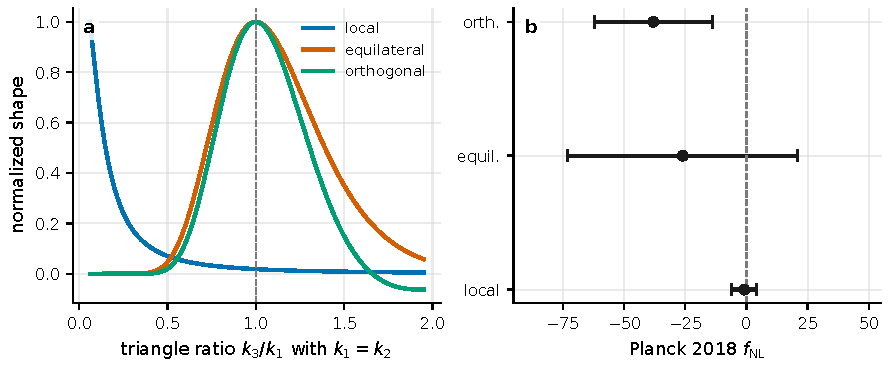
\includegraphics[width=0.9\linewidth]{figures/generated/chapter_16/ch16_non_gaussian_templates.pdf}
\caption{Non-Gaussianity is determined jointly by the triangle configuration and the amplitude. The left panel uses a \(k_1=k_2\) slice to compare the shapes of the local, equilateral, and orthogonal templates; the local type is enhanced in the squeezed limit, and the equilateral type is maximal when the three sides are nearly equal. The right panel gives Planck's representative constraints on the three commonly used \(f_{\rm NL}\), with all error bars consistent with zero.}
\label{fig:e23-nongaussian}
\end{figure}

Tensor perturbations are the most direct CMB target of a quantum-gravity background: they are the primordial gravitational waves produced by inflation, and will leave that ``rare guest,'' the \(B\) mode, in the polarization. People measure them with the ratio of tensor to scalar power:
\begin{equation}
  r(k_*)=\frac{\mathcal P_t(k_*)}{\mathcal P_{\mathcal R}(k_*)},
  \qquad
  \mathcal P_t(k)=A_t\Bigl(\frac{k}{k_*}\Bigr)^{n_t} .
  \label{eq:e23-tensor-r}
\end{equation}
\begin{formulaexplain}
\(r\) is the ratio of the tensor power spectrum to the scalar curvature power spectrum at the pivot \(k_*\), and \(\mathcal P_t\) is described by the amplitude \(A_t\) and the tensor tilt \(n_t\). It compresses the primordial gravitational-wave background into a single number most often cited in CMB \(B\)-mode searches.
\end{formulaexplain}
\(r\) is dimensionless, but the pivot is commonly taken as \(0.002\) or \(0.05\,{\rm Mpc^{-1}}\), and the two \emph{cannot be mixed}. Single-field slow-roll gives another consistency relation \(n_t\simeq-r/8\). \(r\) is precious because it directly converts into the energy scale at which inflation occurred:
\begin{equation}
  V_*^{1/4}\simeq1.06\times10^{16}\,{\rm GeV}\Bigl(\frac{r}{0.01}\Bigr)^{1/4} .
  \label{eq:e23-inflation-scale}
\end{equation}
\begin{formulaexplain}
\(V_*^{1/4}\) is the energy scale of inflation, and \(r\) is the tensor-to-scalar ratio. Note that \emph{fourth root}: even if the upper limit on \(r\) improves by a large margin, the energy-scale constraint tightens only slowly.
\end{formulaexplain}
This expression assumes Einstein gravity, standard slow-roll, and a single energy scale. Planck alone gives \(r_{0.002}<0.10\) (\(95\%\) confidence); combined with the \(B\)-mode polarization of BICEP/Keck it tightens to \(r_{0.002}<0.056\), corresponding to \(V_*^{1/4}<1.6\times10^{16}\,{\rm GeV}\), already approaching the grand-unification scale. BICEP/Keck, combining the 2018-season data with Planck and WMAP, further gives \(r_{0.05}<0.036\), and points out that the current limit is bottlenecked simultaneously by lensing \(B\) modes and Galactic dust (Figure~\ref{fig:e23-bmode}) \citep{2020A&A...641A..10P,2021PhRvL.127o1301A,2019JCAP...02..056A}. In other words, the difficulty of catching that ``rare guest'' lies not in sensitivity but in first ushering out, one by one, the lensing and dust that impersonate it.

\begin{figure}[tbp]
\centering
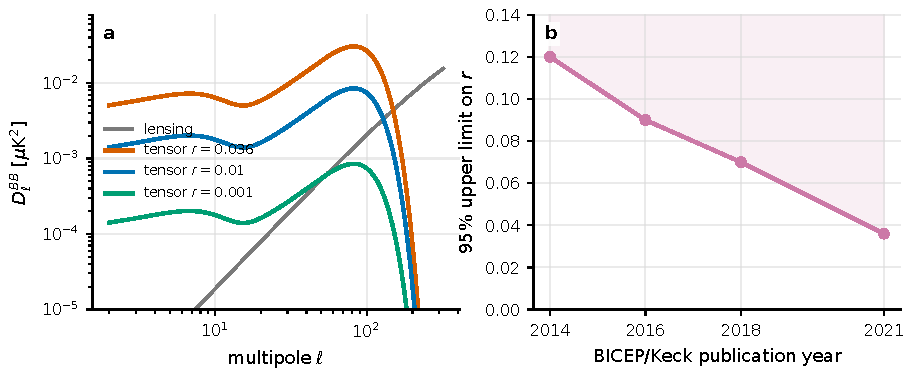
\includegraphics[width=0.9\linewidth]{figures/generated/chapter_16/ch16_bmode_constraints.pdf}
\caption{Tensor modes are constrained mainly through \(B\)-mode polarization. The left panel compares the lensing \(B\) mode with the primordial tensor \(B\) mode for different \(r\): the recombination peak at \(\ell\sim80\) is the main battlefield of ground experiments, while the low-\(\ell\) reionization peak requires large sky areas. The right panel shows the joint constraints of the BICEP/Keck series improving all the way from \(r<0.12\) to the order of \(r_{0.05}<0.036\).}
\label{fig:e23-bmode}
\end{figure}

\section{Photons crossing the universe: polarization is quietly rotated by an angle}
\label{sec:e23-birefringence}

The previous sections were all about ``how the plate was exposed.'' Now switch perspective: light sets out from the last-scattering surface and travels nearly the whole age of the universe to reach us: \textbf{will it be rewritten along the way}? The first precisely testable effect is polarization birefringence (cosmic birefringence): if there exists an extremely light, axion-like (axion) field coupled to the electromagnetic field, the linear-polarization direction of light will be rotated as a whole by a small angle \(\beta\) during propagation. Chapter~\ref{chap:e22} wrote about this polarization channel from the angle of dark matter and axions; here we look at what troubles it meets when it lands on the CMB.

The trouble is first a \emph{calibration} problem. Rotating the polarization direction of the whole sky by \(\beta\) leaks part of the \(E\) mode into the \(B\) mode, producing a signal in the \(EB\) and \(TB\) cross-spectra that should be zero. At small angles this leakage is approximately
\[
  \frac{C_\ell^{EB}}{C_\ell^{EE}-C_\ell^{BB}}\simeq \tfrac12\tan 4\beta\simeq 2\beta .
\]
Plug in a number to feel the order of magnitude: \(0.35^\circ=6.1\times10^{-3}\,{\rm rad}\), so \(2\beta\simeq1.2\%\). This one-percent signal falls precisely at an awkward position: large enough to leave a statistical trace in Planck-level all-sky data, and small enough that \emph{any} inaccuracy in the absolute polarization-angle calibration, dust's own \(EB\), bandpass mismatch, or beam leakage can impersonate it. The lethal part is that a true cosmic rotation angle \(\beta\) and an overall detector polarization-angle miscalibration \(\alpha\) act in almost the same direction in \(EB/TB\), so using only the CMB, what you measure is in fact \(\alpha+\beta\). The key to separating the two is frequency: the cosmological rotation treats all frequencies alike, while the Galactic foreground's polarization varies with frequency, and detector miscalibration is a per-frequency instrumental quantity.

Minami and Komatsu used precisely this ``frequency key,'' relying on the Galactic foreground's different behavior at different frequencies to estimate simultaneously the per-frequency instrumental miscalibration \(\alpha_\nu\) and the cosmic rotation \(\beta\), obtaining \(\beta=0.35\pm0.14^\circ\), and stripping the ground-based angle-calibration systematic of about \(0.28^\circ\) out of the final error. A subsequent analysis using WMAP+Planck PR4, adding a dust \(EB\) model over \(23\text{--}353\,{\rm GHz}\), gives a near-all-sky \(\beta=0.342^{+0.094}_{-0.091}{}^\circ\), with a significance of about \(3.6\sigma\), but polarized dust's own \(EB\), low-frequency synchrotron \(EB\), and independent angle calibration remain the main limitations (Figure~\ref{fig:e23-biref}) \citep{2020PhRvL.125v1301M,2022PhRvD.106f3503E,2022PhRvL.128i1302D,2022NatRP...4..452K}. If interpreted as an axion-like field, the rotation angle comes from the difference of the field value at the two ends of propagation:
\begin{equation}
  \beta=\frac12\,g_{\phi\gamma}\,\bigl[\phi(t_0)-\phi(t_{\rm LSS})\bigr] .
  \label{eq:e23-axion-birefringence}
\end{equation}
\begin{formulaexplain}
\(\beta\) is the global rotation angle of the CMB polarization, \(g_{\phi\gamma}\) is the coupling constant of the field to photons, and the brackets are the difference of the field value between today \(t_0\) and the last-scattering surface \(t_{\rm LSS}\). If the rotation truly comes from an axion-like propagation effect, it should be \emph{approximately frequency-independent}.
\end{formulaexplain}
\(g_{\phi\gamma}\) is in \({\rm GeV^{-1}}\), and \(\phi\) is the effective field value from the last-scattering surface to today. This expression assumes the rotation is approximately isotropic, frequency-independent, and originates from \emph{propagation} rather than an intrinsic \(EB\) at the emission surface. Conversely, the frequency dependence is the best diagnostic: if \(\beta(\nu)\propto\nu^{-2}\), it is more like Faraday rotation through a magnetized plasma (the propagation effect of Chapter~\ref{chap:e21}) than an axion; if \(\beta\) varies with sky region, redshift, or time, then a global angle must be generalized to a direction-dependent or time-dependent correlation function. The pedagogical point here is worth remembering: \textbf{in cosmology, a ``signal'' and a ``calibration error'' often look exactly alike, and separating them relies frequently not on a more sensitive detector, but on cleverer use of extra dimensions like frequency and sky region.}

\begin{figure}[tbp]
\centering
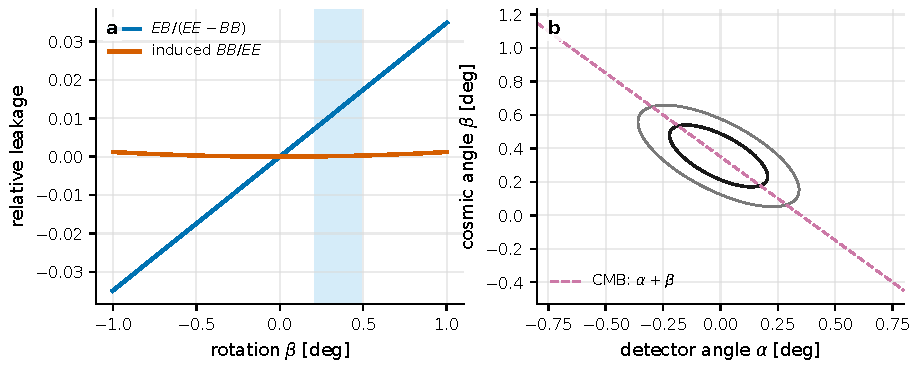
\includegraphics[width=0.9\linewidth]{figures/generated/chapter_16/ch16_birefringence_eb.pdf}
\caption{CMB birefringence puts the polarization-angle error and the cosmological signal on the same plane. The left panel shows the small-angle leakage of \(\beta\) into \(EB\) and induced \(BB\), with the shading marking the order of magnitude of \(\beta=0.35\pm0.14^\circ\); the right panel shows the degeneracy direction of the detector angle \(\alpha\) and the cosmic angle \(\beta\): using only the CMB one measures mainly \(\alpha+\beta\), and only adding foreground frequency information can possibly separate the two.}
\label{fig:e23-biref}
\end{figure}

\section{Arrival time and dispersion: weighing fundamental physics with a cosmological baseline}
\label{sec:e23-timing}

Polarization rotated by an angle is one way light is rewritten en route; \textbf{arrival time pulled apart} is another. This section moves the two tools this book values most, the high-time-resolution photon event table (Chapter~\ref{chap:e13}) and transient sources (the fast radio bursts, gamma-ray bursts, and pulsars of Chapter~\ref{chap:e20}), together onto a cosmological baseline, to test the most fundamental physics: is the speed of light really independent of frequency? Is the photon really strictly massless? Does Lorentz invariance still hold at extremely high energies?

The core of the idea is a criterion plainer than anything: \textbf{if a burst emitted light of various frequencies in the same instant, and they did not arrive simultaneously, then ``something happened along the way''}. To turn this sentence into a measurable, one must write down the relation between frequency and propagation speed. First look at the most familiar, and the first to be subtracted: the tenuous interstellar and intergalactic plasma. The dispersion relation (dispersion relation) an electromagnetic wave satisfies in cold plasma is
\begin{equation}
  \omega^2=\omega_p^2+c^2k^2,
  \qquad
  \omega_p^2=\frac{4\pi n_e e^2}{m_e}.
  \label{eq:e23-plasma-dispersion}
\end{equation}
\begin{formulaexplain}
\(\omega\) is the angular frequency, \(k\) is the wavenumber, \(\omega_p\) is the plasma frequency, \(n_e\) is the electron number density, and \(e,m_e\) are the electron charge and mass (CGS system). The plasma adds a \emph{constant term} \(\omega_p^2\) to the dispersion relation, and the wave can propagate only when \(\omega>\omega_p\).
\end{formulaexplain}
The group velocity (the speed the signal actually travels) is \(v_g={\rm d}\omega/{\rm d}k\). Solving \(k=\sqrt{\omega^2-\omega_p^2}/c\) from \eqref{eq:e23-plasma-dispersion}, differentiating both sides with respect to \(\omega\) and taking the reciprocal, with no skipped step:
\[
  \frac{{\rm d}k}{{\rm d}\omega}=\frac{1}{c}\frac{\omega}{\sqrt{\omega^2-\omega_p^2}}
  \;\Longrightarrow\;
  v_g=\frac{{\rm d}\omega}{{\rm d}k}=c\,\frac{\sqrt{\omega^2-\omega_p^2}}{\omega}
  =c\sqrt{1-\frac{\omega_p^2}{\omega^2}}
  \simeq c\Bigl(1-\frac{\omega_p^2}{2\omega^2}\Bigr),
\]
where the last step used the Taylor expansion \(\sqrt{1-x}\simeq1-x/2\) for \(\omega_p\ll\omega\). The time to travel a path length \(L\) is \(t=L/v_g\simeq(L/c)(1+\omega_p^2/2\omega^2)\). So for two frequencies \(\omega_1<\omega_2\) emitted simultaneously, the difference in arrival times is
\begin{equation}
  \Delta t_{\rm plasma}
  =\frac{L}{2c}\,\omega_p^2\Bigl(\frac{1}{\omega_1^2}-\frac{1}{\omega_2^2}\Bigr)
  \;\propto\;\frac{\int n_e\,{\rm d}l}{\nu^2}
  =\frac{\rm DM}{\nu^2}.
  \label{eq:e23-dm-delay}
\end{equation}
\begin{formulaexplain}
\(\Delta t_{\rm plasma}\) is the arrival-time difference caused by plasma dispersion, \emph{inversely proportional to the square} of the frequency and proportional to the electron column density integrated along the line of sight \(\int n_e\,{\rm d}l\) (that is, the dispersion measure DM, dispersion measure). Low-frequency light travels slower and arrives later.
\end{formulaexplain}
This is precisely the signature feature of fast radio bursts in Chapter~\ref{chap:e20}: a millisecond pulse is stretched on the dynamic spectrum into a \(\nu^{-2}\) bent sweep, and measuring the slope of this bent sweep gives DM, which conversely can weigh the electrons along the way. In the interstellar medium \(n_e\) is about \(10^{-2}\text{--}10^{-1}\,{\rm cm^{-3}}\), and the intergalactic medium is even more tenuous, but with a long baseline the column density is considerable, and millisecond-scale dispersion delays are commonplace.

Wonderfully, \textbf{a massive photon gives a term of exactly the same structure}. The relativistic dispersion relation is \(E^2=(pc)^2+(m_\gamma c^2)^2\): likewise adding a constant term \((m_\gamma c^2)^2\) to the energy--momentum relation, only this time it is the ``rest energy'' rather than the ``plasma frequency'':
\begin{equation}
  E^2=(pc)^2+(m_\gamma c^2)^2 .
  \label{eq:e23-massive-photon}
\end{equation}
\begin{formulaexplain}
\(E=h\nu\) is the photon energy, \(p\) is the momentum, \(m_\gamma\) is the hypothetical photon mass, and \(c\) is the (low-frequency-limit) speed of light. The dispersion relation of a massive photon is mathematically completely isomorphic to that of the plasma: replace \(m_\gamma c^2\) with \(\hbar\omega_p\) and they coincide.
\end{formulaexplain}
Copying the group-velocity derivation above (\(E\) corresponds to \(\hbar\omega\), \(p\) to \(\hbar k\)): \(v_g=\partial E/\partial p=pc^2/E=c\sqrt{1-(m_\gamma c^2/E)^2}\simeq c\,[1-\tfrac12(m_\gamma c^2/E)^2]\), so the arrival-time difference of two energies is
\[
  \Delta t_{m_\gamma}=\frac{L}{2c}\,(m_\gamma c^2)^2\Bigl(\frac{1}{E_1^2}-\frac{1}{E_2^2}\Bigr)
  \;\propto\;\frac{1}{\nu^2}.
\]
It goes as \(\nu^{-2}\) just like the plasma delay, which is both good news and bad news. Good news: any means that can measure a dispersion delay (radio pulsars, fast radio bursts) can inherently set an upper limit on \(m_\gamma\). Bad news: the delays of photon mass and plasma are \emph{completely degenerate}, and one must first subtract the plasma part clean using an independently determined DM (for instance, multiple lines of sight, multiple sources), and only then can the remainder be attributed to \(m_\gamma\). The criterion is still plain: for a burst crossing cosmological distances, if the main pulses at different frequencies are still \emph{consistent to extremely high precision} after subtracting the known DM, then \(m_\gamma\) is forced to an extremely small upper limit: the longer the baseline \(L\), the finer the time resolution, and the wider the frequency span, the more vicious this ruler.

A third possibility hides in higher energies. If Lorentz invariance is very slightly violated as some quantum-gravity energy scale \(E_{\rm QG}\) is approached (Lorentz invariance violation, LIV), the dispersion relation gains an extra correction term that \emph{grows with energy}:
\begin{equation}
  E^2\simeq p^2c^2\Bigl[\,1\pm\Bigl(\frac{E}{E_{\rm QG}}\Bigr)^{n}\Bigr],
  \label{eq:e23-liv-dispersion}
\end{equation}
\begin{formulaexplain}
\(E_{\rm QG}\) is the energy scale at which Lorentz breaking might appear (often taking the Planck scale as reference), \(n\) is the power of the correction (\(n=1\) linear, \(n=2\) quadratic), and \(\pm\) indicates that high-energy photons may travel faster or slower. Its key difference from the mass term is that the correction grows \emph{stronger} with rising energy.
\end{formulaexplain}
Solving \(p\simeq(E/c)[1\mp\tfrac12(E/E_{\rm QG})^n]\) from \eqref{eq:e23-liv-dispersion}, then taking the group velocity \(v=\partial E/\partial p\simeq c\,[1\pm\tfrac{n+1}{2}(E/E_{\rm QG})^n]\), gives the arrival-time difference
\[
  \Delta t_{\rm LIV}\simeq\pm\,\frac{L}{c}\,\frac{n+1}{2}\,\frac{E_2^{\,n}-E_1^{\,n}}{E_{\rm QG}^{\,n}} .
\]
Note that its frequency dependence is \emph{exactly the opposite} of the previous two: plasma and photon mass make the \emph{low} frequency lag (\(\propto\nu^{-2}\)), while LIV makes the \emph{high}-energy photons lead or lag (\(\propto E^{n}\)). This difference in sign and power is the handle for taking the three effects apart. So the natural objects for testing LIV are gamma-ray bursts and high-energy bursts: they simultaneously fling out low-energy and extremely-high-energy photons, and are at cosmological distances, so both \(L\) and \(\Delta E\) are pushed to the extreme; as long as one precisely records the arrival time of each high-energy photon in the event table and aligns it with the low-energy photons, one can push \(E_{\rm QG}\) to a very high lower limit.

Putting the three delays side by side, the methodology of this chapter emerges (in the flavor of Table~\ref{tab:e23-delays}): the same set of ``high-time-resolution event table + cosmologically long baseline'' observations, fed to three models with different frequency dependences, can separately weigh the medium, the photon mass, and spacetime itself. Here we do not quote any specific numerical upper limit: that belongs to the experimental frontier and is strongly dependent on source selection and modeling; what this section teaches you is the \emph{idea}: cosmological distance is not an obstacle, it is a free lever that \emph{amplifies} the faintest fundamental-physics effects into measurable arrival-time differences. The sentence of Chapter~\ref{chap:e13}, ``keep every photon's time tag in the event table,'' at last reveals its greatest ambition here: that time axis is long enough to measure whether the photon has mass, whether spacetime is strictly Lorentz invariant.

\begin{table}[tbp]
\centering
\caption{The three arrival-time differences each have a different frequency dependence, which is precisely the handle for separating them.}
\label{tab:e23-delays}
\begin{tabular}{@{}lll@{}}
\toprule
Effect & Extra term in the dispersion relation & Arrival-time difference vs.\ frequency\\
\midrule
Plasma dispersion & \(+\,\omega_p^2\) (\(\propto n_e\)) & \(\Delta t\propto \nu^{-2}\), low frequency arrives late\\
Photon mass & \(+\,(m_\gamma c^2)^2\) & \(\Delta t\propto \nu^{-2}\), low frequency arrives late (degenerate with plasma)\\
Lorentz breaking & \(\pm\,p^2c^2(E/E_{\rm QG})^n\) & \(\Delta t\propto E^{n}\), high energy leads or lags\\
\bottomrule
\end{tabular}
\end{table}

A word on coherence, in passing. The other side of arrival time being pulled apart is that the phase memory is scrambled. Chapter~\ref{chap:e02} discussed that the time over which a beam of light ``still remembers its phase'' is the coherence time \(\tau_c\simeq1/\Delta\nu\). When light passes through turbulent interstellar/intergalactic plasma, several slightly different paths broaden the pulse and scatter the phase upon arrival, equivalent to wearing down part of the coherence: this is precisely the scattering that the propagation effects of Chapter~\ref{chap:e21} compute in detail. For this chapter, one need only remember a directional conclusion: \textbf{cosmological distance is both a lever that amplifies faint physics and a medium that wears down coherence and broadens pulses}; an instrument seeking to do precision timing or coherence measurement on a cosmological baseline must write both faces into its error budget (Chapter~\ref{chap:e15}).

\section{How the CMB connects with optical quantum astronomy}
\label{sec:e23-bridge}

Finally, let us stitch this chapter back into the whole book. The CMB and the optical quantum astronomy of the earlier parts share the same ``correlation function'' language, but the meaning of the observation differs vastly. Recognizing this difference is what keeps one from casually swapping the ``quantum'' of the two sides.

The first half of this book repeatedly used the second-order coherence function \(g^{(2)}\) to characterize the intensity fluctuations in the detector time series (Chapters~\ref{chap:e08} and \ref{chap:e10}):
\[
  g^{(2)}(\tau)=\frac{\langle I(t)\,I(t+\tau)\rangle}{\langle I\rangle^2}.
\]
Its time delay \(\tau\) and bandwidth \(\Delta\nu\) are both things you can \emph{actively choose}. The basic two-point function of the CMB, by contrast, lives on the celestial sphere, with the number of modes handed out once and for all by the universe:
\begin{equation}
  \langle X_{\ell m}\,Y^*_{\ell'm'}\rangle=C_\ell^{XY}\,\delta_{\ell\ell'}\,\delta_{mm'},
  \qquad
  X,Y\in\{T,E,B,\phi_{\rm lens}\}.
  \label{eq:e23-cmb-correlator}
\end{equation}
\begin{formulaexplain}
\(C_\ell^{XY}\) is the angular power spectrum of two sky fields \(X,Y\), and the two Kronecker deltas indicate that in an isotropic sky different \(\ell,m\) modes are uncorrelated. This is the CMB version of the two-point correlation function.
\end{formulaexplain}
Read them in contrast: the \(\tau\) and \(\Delta\nu\) of \(g^{(2)}\) are set actively by the instrument, and you can change the delay, change the bandwidth, and measure again; the number of modes of \(C_\ell\) is given by the universe, and the observer can only change the sky mask, frequency combination, beam, noise weighting, and foreground model. The CMB cannot, like a laboratory, modulate the source, re-prepare the initial state, or rerun once: it gives the statistical information of the early field modes, a shadow projected onto \(T/E/B\), lensing, and higher-order correlations.

What truly turns this shadow into cosmological numbers is the map-level (map-level) likelihood. All the frequency maps, polarization maps, and external tracers flow into the same data vector \(\bm d\):
\begin{equation}
  \bm d=\bm P\,[\,\bm s_{\rm CMB}(\bm\theta)+\bm s_{\rm fg}(\bm\eta)\,]+\bm n,
  \qquad
  -2\ln\mathcal L=(\bm d-\bm m)^{\mathsf T}\,C^{-1}\,(\bm d-\bm m)+\ln\det C .
  \label{eq:e23-cmb-likelihood}
\end{equation}
\begin{formulaexplain}
\(\bm d\) is the map-level data vector, \(\bm P\) is the observation/mapping operator (including beam, mask, scanning strategy, and bandpass), \(\bm s_{\rm CMB}\), \(\bm s_{\rm fg}\) are the cosmic signal and foreground, and \(\bm n\) is the noise. The likelihood puts the model residual and the total covariance \(C\) together, which is the working form for inferring cosmological parameters from a sky map.
\end{formulaexplain}
Here \(\bm\theta\) are the cosmological parameters (such as \(A_s,n_s,\Omega_bh^2,\Omega_ch^2,r,\beta\)), \(\bm\eta\) are the foreground parameters (dust temperature and spectral index, synchrotron spectral index, spatial decorrelation, etc.), and the covariance \(C\) holds in one go the instrument noise, sample variance, foreground residuals, and calibration uncertainty. The differences between Planck, the Simons Observatory, and future CMB-S4- and LiteBIRD-class experiments lie mainly in \(\bm P\), \(C\), frequency coverage, angular resolution, and controllable systematic errors \citep{2016A&A...594A..13P,2016A&A...594A..20P,2017MNRAS.472.1195C,2019JCAP...02..056A,2020A&A...641A...6P}.

When reading the CMB literature, units and pivots are the most treacherous; three parting reminders. First, \(T_0\) is in K, fluctuation maps are commonly in \(\mu{\rm K}\), and the primordial \(\mathcal P_{\mathcal R}\) is dimensionless: \(A_s\sim2.1\times10^{-9}\) cannot be directly compared with \(D_\ell^{TT}\sim5000\,\mu{\rm K}^2\), with a whole radiation transfer function in between. Second, \(k\) (in \({\rm Mpc^{-1}}\)) and \(\ell\) (angular mode number) are related through \(\ell\simeq k\,D_A(z_*)\), where \(D_A(z_*)\) is the comoving angular diameter distance of the last-scattering surface. Third, the pivot of \(r\) is not unified, \(r_{0.002}\) and \(r_{0.05}\) are not the same number, and especially when \(n_t\) is left free they cannot be mixed. The quantum-network telescope of Chapter~\ref{chap:e24} will bring the discussion back to an experimental system that can be actively manipulated; the CMB stands at the opposite limit: the initial state cannot be redone, the light path cannot be reset, yet it has printed, neat and orderly, the statistical trace left by that quantum fluctuation of the early universe onto a plate we only read today.

\section*{Chapter Summary}
\addcontentsline{toc}{section}{Chapter Summary}

\begin{itemize}
\item \textbf{The CMB is first a light field.} The mean is a blackbody of \(T_0=2.7255\,{\rm K}\), and the information is in the angular fluctuations of \(\Delta T/T\sim10^{-5}\) and the polarization on top of it; the angular power spectrum \(C_\ell\) is the core two-point statistic, and low \(\ell\) has an unavoidable cosmic variance \(\sqrt{2/[(2\ell+1)f_{\rm sky}]}\).
\item \textbf{The seeds of the primordial fluctuations are quantum.} Inflation treats each mode as a time-varying-frequency oscillator, and after horizon exit the curvature perturbation is frozen; in quantum-optics language, this is a two-mode squeezed state of \(\bm k\) and \(-\bm k\), and the fixed phase explains the string of acoustic peaks.
\item \textbf{Decoherence turns quantum into classical.} Entanglement with the environment makes the off-diagonal terms of the reduced density matrix be squeezed dead by \(\exp[-\Gamma_k(q-q')^2]\), and when \(\Gamma_k(\Delta q)^2\gg1\), the power spectrum can be computed as a classical random field: this is the exact meaning of ``quantum fluctuations becoming classical density perturbations.''
\item \textbf{Higher-order statistics and tensor modes test ``how they were produced.''} \(f_{\rm NL}\) is consistent with zero, supporting the simplest single-field slow-roll; \(r_{0.05}<0.036\) pushes the primordial gravitational waves (that \(B\)-mode rare guest in the polarization) down to an energy scale \(\lesssim1.6\times10^{16}\,{\rm GeV}\), with the difficulty being the subtraction of lensing and dust.
\item \textbf{Light is rewritten en route.} Polarization may be rotated by \(\beta\sim0.3^\circ\) (birefringence), and separating the cosmic angle from the instrument angle relies on the frequency dimension; arrival time may be pulled apart, with plasma and photon mass giving a \(\nu^{-2}\) delay that is mutually degenerate, and Lorentz breaking giving an \(E^{n}\) delay: the difference in frequency dependence is precisely the handle for taking them apart.
\item \textbf{Cosmological distance is a free lever.} A high-time-resolution event table (Chapter~\ref{chap:e13}) together with a cosmologically long baseline and transient sources can amplify the faintest effects, such as photon mass and Lorentz breaking, into measurable arrival-time differences, at the price that the same distance also wears down coherence and broadens pulses.
\end{itemize}

\medskip
\noindent\textbf{Questions to Ponder.}
\begin{enumerate}
\item The cosmic-variance relative error at all-sky \(\ell=2\) is about \(63\%\). If one observes only half the sky (\(f_{\rm sky}=0.5\)), what does this error become? Why can no amount of detector sensitivity recover this part of the information?
\item Both plasma dispersion and photon mass give a \(\nu^{-2}\) arrival delay. If you have data on the \emph{same batch} of radio bursts in \emph{different lines of sight}, how would you use the variation of DM to strip the possible photon-mass share out of the plasma?
\item A true cosmic polarization rotation \(\beta\) and a detector angle miscalibration \(\alpha\) both manifest as an \(EB\) signal in the CMB. Why can ``using foregrounds at different frequencies'' separate the two, whereas ``making the detector more sensitive'' cannot?
\end{enumerate}


% ============================================================
\part{Frontiers, Case Studies, and Practice}
\chapter{Quantum-Network Telescopes}
\label{chap:e24}

\begin{chapteropening}
In Chapter \ref{chap:e09} we learned to combine the light of two telescopes and count fringes: the fringe visibility is the complex visibility \(V\), and \(V\) encodes the angular structure of the star. But that chapter also left us with a heavy footnote: to keep the fringes stable, the optical path difference between the two arms must be locked to a precision far smaller than one wavelength, and any loss along either arm \emph{directly devours the already scarce starlight photons}. Stretch the baseline to a few kilometers, or a few tens of kilometers, and both requirements spiral out of control. This chapter asks a bold question: can we avoid \emph{hauling the unknown starlight over long distances} and yet still ``join'' two widely separated telescopes into a single instrument? The answer comes from quantum information: an \textbf{entanglement resource} that is prepared in advance, can be verified, and can be redone if it fails, together with \textbf{quantum memory} and a \textbf{quantum repeater}, lets the two ends ``share'' the phase relation of a single photon without forcing that fragile starlight photon to make the whole journey itself. This route is not yet a mature instrument but a feasibility ledger that must be worked out line by line; this chapter builds that ledger from the ground up and places it side by side with the intensity interferometry of Chapter \ref{chap:e10}.
\end{chapteropening}

\section{Why long-baseline amplitude interferometry is throttled by photon loss}
\label{sec:e24-why-loss}

Let us strip the problem down to its essence. What we really want to preserve is not ``more light'' but \emph{the phase of first-order coherence}. Imagine a point source in the sky; within one coherence time \(\tau_c\simeq1/\Delta\nu\) (Chapter \ref{chap:e02}) a single photon from it happens to fly to the telescope array. The key fact about extremely faint starlight is this: the mean number of photons from the object per time window, \(\epsilon\ll1\), is tiny: the vast majority of windows are empty, and now and then a single window contains just one photon. This one photon, if it has not been contaminated by any ``which-path'' information before reaching the detector, is \emph{not} a classical particle that ``already belongs to the left telescope'' or ``already belongs to the right telescope''; it is a quantum superposition of the left and right receiving paths:

\begin{equation}
  |\psi_\star\rangle
  =
  \frac{|1\rangle_L|0\rangle_R
  +
  e^{i\phi}\,|0\rangle_L|1\rangle_R}{\sqrt2},
  \qquad
  \phi=\frac{2\pi\,\bm{B}\cdot\bm{\theta}}{\lambda}.
  \label{eq:e24-stellar-single-photon}
\end{equation}
\begin{formulaexplain}
\(|\psi_\star\rangle\) is the path-superposition state of one starlight photon between the left and right apertures; \(|1\rangle_L|0\rangle_R\) means ``one photon on the left, nothing on the right,'' and the other term is the reverse. \(\phi\) is the geometric phase fixed by the baseline \(\bm{B}\), the source angular position \(\bm{\theta}\), and the wavelength \(\lambda\). What amplitude interferometry must preserve is precisely this \(\phi\).
\end{formulaexplain}

Here \(|1\rangle_L|0\rangle_R\) is number-state notation (Chapter \ref{chap:e05}): the subscripts \(L,R\) label the left and right spatial modes, and the numbers in the kets are the photon numbers in those modes. \(\bm{B}\) is the projected baseline (in cm, ranging in magnitude from \(10^2\,\mathrm{cm}\) to \(10^7\,\mathrm{cm}\)), \(\bm{\theta}\) is the angular position of the point source relative to the phase center (dimensionless radians), and \(\lambda\) is the wavelength (visible light \(\sim6\times10^{-5}\,\mathrm{cm}\)). The phase \(\phi\) is dimensionless and purely geometric: it is exactly the phase in the fringes of Chapter \ref{chap:e09}, only now written in the language of a single-photon superposition state.

A real star is not a point but a sum of many mutually incoherent point sources (this is precisely the starting point of the van Cittert--Zernike theorem in Chapter \ref{chap:e10}). Each subsource \(j\) gives its own pure state \eqref{eq:e24-stellar-single-photon} with phase \(\phi_j\); the incoherent superposition weights these pure states by brightness and sums them into a mixed state. After summation, what appears in the off-diagonal element is exactly the brightness-weighted average of those phase factors \(\langle e^{i(\phi_j-\phi_k)}\rangle\), which converges to precisely the complex visibility \(V\) of Chapter \ref{chap:e10}. Restricting to the single-photon subspace \(\{|10\rangle,|01\rangle\}\), the density matrix is

\begin{equation}
  \rho_1
  =
  \frac{1}{2}
  \begin{pmatrix}
  1 & V\\[2pt]
  V^* & 1
  \end{pmatrix}_{\{|10\rangle,\,|01\rangle\}} ,
  \qquad
  V=|V|\,e^{i\arg V}.
  \label{eq:e24-single-photon-density}
\end{equation}
\begin{formulaexplain}
\(\rho_1\) is the density matrix of the single-photon subspace; the diagonal elements \(\tfrac12\) only say ``the photon can appear at either telescope,'' while the off-diagonal element \(V\) is the complex visibility, carrying the coherent phase and angular structure of the source. \(|V|\) falls from 1 (a point source) to 0 (a source large enough to be resolved out), and the phase gives the source's position and asymmetry.
\end{formulaexplain}

Compare this with Eq.\ \eqref{eq:e10-gamma12} of Chapter \ref{chap:e10}: there the complex visibility \(\gamma^{(1)}_{12}\) is defined via the time average of the two field arms; the \(V\) here is the very same quantity, merely relocated to the off-diagonal element of the single-photon density matrix. The physical meaning is identical: \emph{to measure \(V\) is to measure the star}. The traditional amplitude-interferometry approach sends the two spatial modes \(L,R\) through fibers or free-space optical paths to \emph{the same} beamsplitter, turning \(\phi\) into countable fringes. The trouble lies precisely in this ``send to the same beamsplitter'' step: if one arm travels a lossy link of length \(L\), the single-photon transmittance is

\begin{equation}
  \eta_{\rm ch}(L)=10^{-\alpha_{\rm dB}L/10}.
  \label{eq:e24-link-loss}
\end{equation}
\begin{formulaexplain}
\(\eta_{\rm ch}\) is the link transmittance (dimensionless, \(0\) to \(1\)); \(\alpha_{\rm dB}\) is the loss in decibels per kilometer (units \(\mathrm{dB\,km^{-1}}\)), and \(L\) is the link length (km). The decibel loss makes the transmittance decay \emph{exponentially} with distance: this is the core bottleneck of direct optical combination over long baselines.
\end{formulaexplain}

The decibel is a logarithmic scale: \(10\,\mathrm{dB}\) means attenuation to \(1/10\), and \(20\,\mathrm{dB}\) means \(1/100\). Plug in real numbers to get a feel. Visible light in ordinary fiber suffers losses as high as \(20\)--\(30\,\mathrm{dB\,km^{-1}}\); over \(1\,\mathrm{km}\) only \(10^{-2}\) to below \(10^{-3}\) survives, and the starlight, already at \(\epsilon\ll1\), is nearly wiped out. Switch to the \(1550\,\mathrm{nm}\) telecom band, and the best fibers reach \(\sim0.2\,\mathrm{dB\,km^{-1}}\); but starlight does not naturally live in this band, so one must first do frequency conversion, coupling, and phase stabilization, each step multiplying in another sub-unity efficiency. A clear-sky free-space link can be taken as \(\sim0.5\,\mathrm{dB\,km^{-1}}\) for order-of-magnitude estimates, but the losses from atmospheric turbulence and pointing errors do not follow this clean exponential law \citep{2012PhRvL.109g0503G,2019PhRvL.123g0504K,2024SPIE13095E..1NR}. In a word: \emph{the more you want to lengthen the baseline, the farther you must send this already scarce starlight photon, and the probability of losing it rises exponentially with distance}.

\begin{figure}[tbp]
\centering
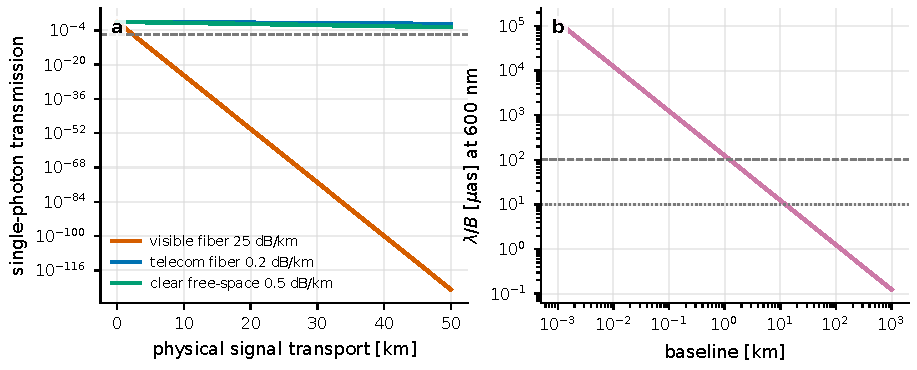
\includegraphics[width=0.94\linewidth]{figures/generated/chapter_17/ch17_architecture_loss.pdf}
\caption{The allure and the difficulty of long baselines come from the same dimension. The left panel plots the link loss for several ways of ``directly transmitting single-photon starlight'' as transmittance: visible-light fiber is already severely attenuated on kilometer scales, and even telecom-band fiber becomes expensive at hundred-kilometer scales. The right panel gives the angular-resolution scale \(\lambda/B\): \(600\,\mathrm{nm}\) light on a \(1\,\mathrm{km}\) baseline reaches the hundred-microarcsecond level, and a \(100\,\mathrm{km}\) baseline enters the microarcsecond regime.}
\label{fig:e24-architecture-loss}
\end{figure}

So why go to such lengths to stretch the baseline? Because the fundamental scale of angular resolution recognizes only the baseline length \(B\):

\begin{equation}
  \theta_{\rm res}\sim\frac{\lambda}{B}
  =124\,\mu\mathrm{as}
  \left(\frac{\lambda}{600\,\mathrm{nm}}\right)
  \left(\frac{1\,\mathrm{km}}{B}\right).
  \label{eq:e24-resolution-scale}
\end{equation}
\begin{formulaexplain}
\(\theta_{\rm res}\) is the angular-resolution scale of the interferometer (here in microarcseconds \(\mu\mathrm{as}\)), and \(B\) is the baseline length. The longer the baseline, the finer the angular structure that can be resolved. What the quantum-network scheme pursues is precisely pushing \(B\) to kilometers and beyond \emph{without hauling unknown starlight over long distances}.
\end{formulaexplain}

Set the ratios in the parentheses to 1 and you read off the benchmark of \(124\,\mu\mathrm{as}\); \(B=10\,\mathrm{km}\) gives \(12\,\mu\mathrm{as}\), and \(B=100\,\mathrm{km}\) gives \(1.2\,\mu\mathrm{as}\). For reference, the largest optical interferometric arrays (such as CHARA) have baselines of a few hundred meters and reach only the milliarcsecond level. The appeal of the quantum-network telescope is locked to this scale: it may not improve the sensitivity of a single aperture, but it could push optical/near-infrared interferometry from a few hundred meters all the way to kilometers, tens of kilometers, or longer. Intensity interferometry (HBT) of Chapter \ref{chap:e10} in fact already sidestepped the hurdle of optical-path transport: it does not combine beams but records intensity fluctuations locally and correlates them offline, and so is almost immune to atmospheric jitter, at the price of giving mainly \(|V|^2\) and losing the phase. The ambition of the quantum-network route is different: it wants to \emph{preserve the phase of first-order coherence} while \emph{not hauling unknown starlight over long distances}.

\section{Pre-shared entanglement: replacing what must be transported}
\label{sec:e24-gjc}

The central trick was devised by Gottesman--Jennewein--Croke: since hauling the fragile, unknown starlight over long distances is so costly, \emph{don't haul it}; instead, transport a ``laboratory photon'' that we fully control, can verify, and can remake if it breaks. This laboratory photon is prepared in advance in a known path-entangled state:

\begin{equation}
  |\Phi_\delta\rangle
  =
  \frac{|1\rangle_L|0\rangle_R
  +
  e^{i\delta}\,|0\rangle_L|1\rangle_R}{\sqrt2}.
  \label{eq:e24-lab-entangled-photon}
\end{equation}
\begin{formulaexplain}
\(|\Phi_\delta\rangle\) is the pre-shared laboratory path-entangled photon; its form is identical to the starlight state \eqref{eq:e24-stellar-single-photon}, except that the phase \(\delta\) is entirely under our control. It takes over the task of ``hauling unknown starlight over long distances'': this entanglement can be distributed in advance and verified afterward, and if it fails it is simply discarded and redone, never touching the precious starlight.
\end{formulaexplain}

Notice how strikingly similar the structures of \(|\Phi_\delta\rangle\) and \(|\psi_\star\rangle\) are: both are superpositions of ``one on the left / one on the right,'' differing only in that one phase is the heaven-set \(\phi\) and the other the human-set \(\delta\). This is the whole trick: let the \emph{known} \(\delta\) interfere locally with the \emph{unknown} \(\phi\), thereby reading out \(\phi\) (that is, \(V\)), while neither end has to send its own photon to the other.

How, concretely, do we read it? After the starlight photon arrives, each of the two stations \emph{locally} feeds its ``starlight mode'' and its ``laboratory entangled mode'' together into a beamsplitter, then keeps only certain \emph{coincidence} events, such as ``the left station detects one photon and the right station also detects one.'' The beamsplitter acts just as in Chapter \ref{chap:e09}: it linearly combines the two input amplitudes into the two output ports \((\text{starlight}\pm\text{laboratory})/\sqrt2\), so the field at each output is a \emph{coherent superposition} of the two path amplitudes. Once this is done, ``whether the photon was starlight or laboratory light, and which path it took'' is \emph{which-path information that gets erased}, leaving only the phase relation \(\phi-\delta\) between the two paths. The probability of a coincidence at both ends is proportional to the modulus squared of the coherently superposed amplitudes of these two erased paths; substituting the starlight state \eqref{eq:e24-stellar-single-photon} and the laboratory state \eqref{eq:e24-lab-entangled-photon} and expanding, the \emph{cross term} in the modulus squared is exactly \(\mathrm{Re}(V e^{-i\delta})\), and this is the carrier of the interference information. The full two-mode beamsplitter-plus-coincidence algebra is a standard result in quantum-optics textbooks; here we simply give its conclusion: the probabilities of the correlated and anti-correlated coincidence clicks are

\begin{equation}
  P_{\pm}(\delta)
  =
  \frac{1}{2}
  \Bigl[\,1\pm\mathrm{Re}\!\left(V\,e^{-i\delta}\right)\Bigr].
  \label{eq:e24-gjc-probability}
\end{equation}
\begin{formulaexplain}
\(P_\pm(\delta)\) are the probabilities of the two classes of coincidence clicks, \(V\) is the stellar complex visibility, and \(\delta\) is the laboratory phase that we can tune. Changing \(\delta\) is like scanning a reference phase: the click rate oscillates sinusoidally with \(\delta\), and from the amplitude and phase of the oscillation one reads out the real and imaginary parts of \(V\).
\end{formulaexplain}

Substituting \(V=|V|e^{i\arg V}\), we have \(\mathrm{Re}(Ve^{-i\delta})=|V|\cos(\arg V-\delta)\), so the \emph{oscillation depth} of \(P_\pm(\delta)\) as \(\delta\) varies is exactly \(|V|\), and its \emph{phase} is exactly \(\arg V\). In other words, sweeping \(\delta\) once measures the entire complex visibility, exactly the same physics as scanning the optical path difference to obtain fringes in Chapter \ref{chap:e09}, except that the reference phase is now provided by a local entanglement resource, and the starlight photon never leaves its own station from start to finish. This ``local beamsplitter + coincidence detection'' is called a \textbf{Bell-state measurement} in quantum information: it projects the two photons onto a basis of maximally entangled two-mode states. Unfortunately linear optics can unambiguously distinguish only some of the click combinations, so only about half of the usable starlight events enter the estimate; if one could perform a complete Bell-state measurement or more elaborate quantum processing, this \(50\%\) loss could in principle be avoided \citep{1982Natur.299..802W,1993PhRvL..70.1895B,2012PhRvL.109g0503G}.

A problem follows, and a hard one: the \textbf{resource rate}. This direct GJC route demands that \emph{every coherence-time window that might contain starlight have a matching entangled photon prepared in advance}. The bandwidth \(\Delta\nu\) sets the coherence time to about \(1/\Delta\nu\), so the number of time windows to cover per second is about \(\Delta\nu\). Take \(\Delta\nu=10\,\mathrm{GHz}\) and that is \(10^{10}\) windows per second, meaning you need a source that spits out \(10^{10}\) high-quality entangled photon pairs per second. Astronomical roadmaps (Rajagopal et al.) make it explicit that the best current entangled-photon sources fall far short of this rate; direct GJC is therefore better suited as a \emph{short-baseline in-sky proof of principle}, and in the near term it cannot yet replace existing optical interferometric arrays \citep{2024SPIE13095E..1NR,2012PhRvL.109g0503G}.

The scheme of Khabiboulline--Borregaard--De Greve--Lukin cleverly turns the very weakness of starlight to advantage. Since each long measurement window contains on average only \(\epsilon\ll1\) correlated starlight photons, one slices the window into \(M\sim1/\epsilon\) finer time bins, so that \emph{at most one bin} actually contains a photon. To record ``which bin the photon landed in,'' the clumsy way (a unary code, one bit per bin) needs \(M\) entangled pairs; the clever way (a binary code that encodes the arrival time in binary) needs only

\begin{equation}
  n_{\rm mem}
  =
  \bigl\lceil\log_2(M+1)\bigr\rceil
  \simeq
  \bigl\lceil\log_2(1/\epsilon)\bigr\rceil
  \label{eq:e24-binary-timebin}
\end{equation}
\begin{formulaexplain}
\(n_{\rm mem}\) is the number of storage qubits required, \(M\) is the number of time bins, and \(\epsilon\) is the mean number of starlight photons per bin. The \emph{sparsity} of faint light compresses the resource requirement from \(M\) entangled pairs down to about \(\log_2 M\) storage bits: an exponential saving.
\end{formulaexplain}

storage qubits, with each bit using one entangled pair to perform a nonlocal \textbf{parity check}. The scaling immediately becomes enticing: if \(M=10^6\), only about \(20\) qubits are needed to encode the arrival time, whereas a unary code would require a million entangled pairs. A representative worked example from the paper is: for a bandwidth \(\Delta f=1\,\mathrm{MHz}\) and a \(1\,\mathrm{s}\) measurement window, \(N=10^6\) time bins correspond to \(\log_2 N\simeq20\) qubits; in an astronomical example with a \(10\)th-magnitude star, \(10\,\mathrm{m^2}\) collecting area, and \(10\,\mathrm{GHz}\) detection bandwidth, the inferred resource target is roughly \(20\)--\(30\) qubits plus an entanglement-supply rate of \(\sim200\,\mathrm{kHz}\). A supplementary analysis by Stas et al.\ also uses \(20\) SiV nodes, a \(1\,\mathrm{kHz}\) zero-distance entanglement rate, and a \(1\,\mathrm{s}\) window to demonstrate a viable path toward this logarithmic scaling \citep{2019PhRvL.123g0504K,2022PhRvA.106c2424C,2026Natur.651..326S,2024SPIE13095E..1NR}.

\begin{figure}[tbp]
\centering
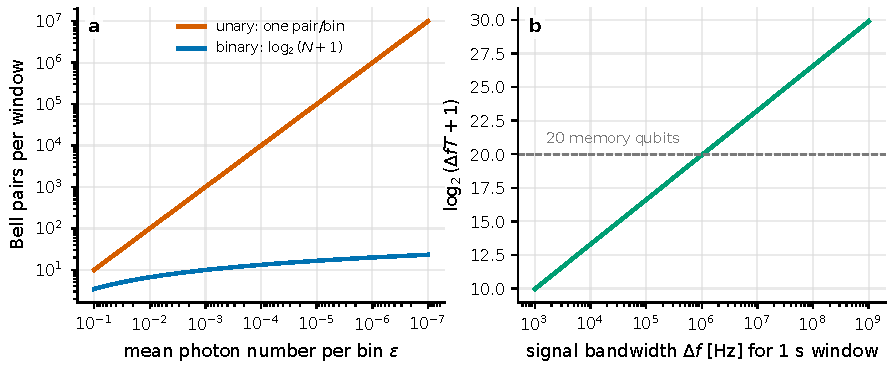
\includegraphics[width=0.94\linewidth]{figures/generated/chapter_17/ch17_timebin_scaling.pdf}
\caption{It is precisely because ``starlight is weak'' that time-bin encoding becomes meaningful. The left panel compares the entangled-pair requirements of unary versus binary encoding: when the mean photon number per bin \(\epsilon\) is small, \(M\sim1/\epsilon\) bins can be labeled with only \(\log_2(M+1)\) storage qubits. The right panel shows that in a \(1\,\mathrm{s}\) measurement window, a \(1\,\mathrm{MHz}\) bandwidth corresponds to about \(10^6\) bins, that is, about \(20\) qubits.}
\label{fig:e24-timebin}
\end{figure}

The underlying communication technology that supports all of this is the \textbf{quantum repeater}. Why can we not amplify a quantum state and send it far, the way we boost an electrical signal? Because the \emph{no-cloning theorem} forbids perfectly copying an unknown quantum state \citep{1982Natur.299..802W}, while loss rises exponentially with distance (Eq.\ \eqref{eq:e24-link-loss}). The repeater's idea is divide and conquer: cut the long distance into many short segments, first establish entanglement within each short segment (short segments have small loss and high success probability), then use \textbf{entanglement swapping} to ``relay'' the entanglement of adjacent segments into entanglement spanning the whole distance. An ideal repeater can trade exponential loss for much gentler resource scaling, but a real system must still face a chain of penalties: the success probability of the Bell-state measurement, the storage lifetime, dark counts, gate fidelity, and frequency conversion. The DLCZ atomic-ensemble protocol, quantum-internet roadmaps, and quantum-memory reviews all place \emph{storage} squarely at the center of the resource budget, because the job of storage is to \emph{align in time} these probabilistically successful events \citep{1998PhRvL..81.5932B,2001Natur.414..413D,2011RvMP...83...33S,2008Natur.453.1023K,2012IEEEN..26d..59V,2006quant.ph..7182U}.

\section{The resource ledger: how entanglement rate, storage time, and fidelity close together}
\label{sec:e24-budget}

Whichever of the above schemes we choose, in the end all return to the same ledger. Angular resolution is handed to us for free by \(B\) (Eq.\ \eqref{eq:e24-resolution-scale}), but \emph{whether an observation is actually possible} requires the entanglement-supply rate, the storage time, the fidelity, and the starlight event rate to all meet their targets \emph{simultaneously}; if even one falls short, the phase lever of the long baseline cannot be pried loose.

The first item is the \textbf{entanglement-supply rate}. Let the accepted effective starlight event rate be \(R_\star\), and let each event consume on average \(n_{\rm pair}\) entangled pairs; then

\begin{equation}
  R_{\rm ent}
  \gtrsim
  \frac{n_{\rm pair}\,R_\star}{p_{\rm ready}} .
  \label{eq:e24-entanglement-rate}
\end{equation}
\begin{formulaexplain}
\(R_{\rm ent}\) is the required entanglement-supply rate (units Hz), \(R_\star\) is the effective starlight event rate (Hz), \(n_{\rm pair}\) is the number of entangled pairs consumed per event, and \(p_{\rm ready}\) is the probability that an entangled pair is ready when the starlight arrives. It \emph{directly translates} the astronomical event rate into a throughput requirement on the quantum network.
\end{formulaexplain}

To understand this equation, one must first be clear about \(R_\star\): it is \emph{not} the total photon rate received by the telescope but the rate of events that entered the target spatial mode, frequency channel, and polarization channel, fell within the time window, and passed quality selection: the events \emph{actually usable}. The closer \(p_{\rm ready}\) is to 1, the more the entanglement resource is essentially always on standby, and the less is wasted. The lesson of this equation is direct: for a bright, broadband source, \(R_\star\) is enormous, and direct GJC is crushed by the resource rate; for a narrowband, faint source, \(R_\star\) is small, and only then does a storage-assisted scheme have a chance to trade a lower \(R_{\rm ent}\) for a long baseline.

The second item is the \textbf{storage time}. At the very least, the quantum state or measurement record must be kept until the classical communication and the nonlocal check are both complete:

\begin{equation}
  T_{\rm mem}
  \gtrsim
  \max\!\left[\frac{B}{c},\,T_{\rm ent},\,T_{\rm proc},\,T_{\rm win}\right].
  \label{eq:e24-memory-time}
\end{equation}
\begin{formulaexplain}
\(T_{\rm mem}\) is the minimum time for which the quantum memory must remain coherent, equal to the maximum of the four terms on the right: the baseline light-travel time \(B/c\), the entanglement-generation time \(T_{\rm ent}\), the processing time \(T_{\rm proc}\), and the measurement window \(T_{\rm win}\). The real bottleneck is often \emph{not} \(B/c\) but synchronization and the time-bin window.
\end{formulaexplain}

Plug in numbers and it becomes clear: the light-travel time \(B/c=3.3\,\mu\mathrm{s}\times(B/\mathrm{km})\), so a \(100\,\mathrm{km}\) baseline needs only \(0.33\,\mathrm{ms}\) of light-travel time, which sounds easy. But the Khabiboulline-type binary time-bin scheme, in order to cover narrowband faint light, may need a measurement window \(T_{\rm win}\) as long as \(\sim1\,\mathrm{s}\), several orders of magnitude more demanding than the light-travel time. Quantum-memory hardware is usually described by six figures of merit: fidelity, efficiency, storage time, bandwidth, multimode capacity, and operating wavelength. For single-photon storage, the \emph{conditional fidelity} is the overlap between the retrieved wave packet and the written one, and the \emph{efficiency} is the probability of successfully retrieving the photon; once one wants to interfere the stored photon with starlight, the \emph{product} of these two, plus phase noise and mode matching, directly lowers the final visibility \citep{2009NaPho...3..706L,2010EPJD...58....1S,2016JMOp...63.2005H}.

\begin{figure}[tbp]
\centering
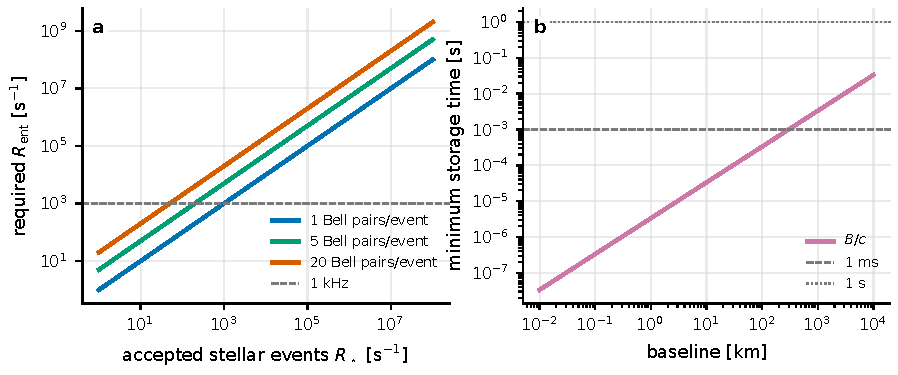
\includegraphics[width=0.94\linewidth]{figures/generated/chapter_17/ch17_entanglement_resources.pdf}
\caption{The entanglement rate and storage time give the first layer of resource-closure conditions. The left panel converts the accepted starlight event rate \(R_\star\) into the required entangled-pair rate: the more pairs each event consumes, the higher the demand line rises. The right panel converts the baseline into light-travel time \(B/c\): for kilometer-scale baselines, the light-travel time is only microseconds to milliseconds, but narrowband storage schemes are often dictated by the measurement window and the entanglement-generation time.}
\label{fig:e24-entanglement-resources}
\end{figure}

The third item is the \textbf{fidelity}. The resource budget often simply \emph{multiplies} several major penalty factors along the link to obtain a rough effective fidelity:

\begin{equation}
  F_{\rm eff}
  \simeq
  F_{\rm Bell}\,
  \eta_{\rm write}\,\eta_{\rm read}\,\eta_{\rm conv}\,
  e^{-T/T_2}\,
  (1-p_{\rm dark})\,
  M_{\rm mode}.
  \label{eq:e24-effective-fidelity}
\end{equation}
\begin{formulaexplain}
\(F_{\rm eff}\) is a rough effective resource quality, multiplying together the entangled-pair fidelity \(F_{\rm Bell}\), the write/read efficiencies, the frequency-conversion efficiency, the storage decoherence \(e^{-T/T_2}\), the dark-trigger term \((1-p_{\rm dark})\), and the mode matching \(M_{\rm mode}\). \emph{Any one factor being low lowers the final visibility multiplicatively}.
\end{formulaexplain}

Naming the units one by one: \(F_{\rm Bell}\) (dimensionless, \(\le1\)) is the fidelity of the pre-shared entangled pair; \(\eta_{\rm write},\eta_{\rm read}\) (dimensionless) are the write and read efficiencies; \(\eta_{\rm conv}\) is the frequency-conversion efficiency; \(T_2\) is the storage coherence time (units s), \(T\) is the actual storage duration; \(p_{\rm dark}\) is the equivalent dark-trigger probability; and \(M_{\rm mode}\le1\) denotes the degree of matching across the four types of mode: frequency, time, polarization, and space. This is not a complete quantum-channel model, but it has a virtue: it \emph{exposes the bottleneck at a glance}. Looking at the decoherence factor alone, \(T/T_2=1\) already gives a factor of \(e^{-1}\simeq0.37\); further assume \(F_{\rm Bell}=0.8\), read and write \(0.7\) each, and conversion \(0.8\) (not yet counting dark counts and mode mismatch), and multiplying, \(0.8\times0.7\times0.7\times0.8\simeq0.31\), the final visibility is already down to around thirty percent. This is why such schemes cannot fixate on ``how enticing the angular resolution is'' but must make every factor \emph{simultaneously} close.

\begin{figure}[tbp]
\centering
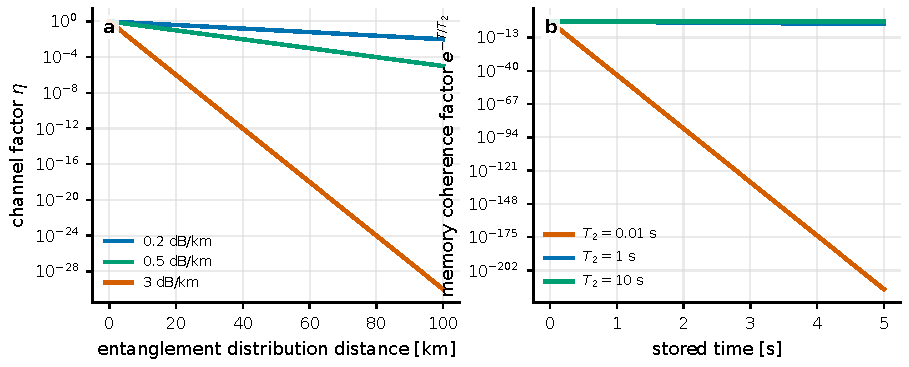
\includegraphics[width=0.94\linewidth]{figures/generated/chapter_17/ch17_fidelity_distance.pdf}
\caption{The effective resource quality is determined jointly by the link and the storage. The left panel gives the fall of the channel factor with distance for various \(\mathrm{dB\,km^{-1}}\) losses; the right panel gives the fall of the storage-decoherence factor \(e^{-T/T_2}\) with storage duration. However enticing its angular resolution, a long-baseline scheme must make the entangled-pair fidelity, the read/write efficiency, the frequency conversion, and the storage coherence all meet their targets \emph{together}.}
\label{fig:e24-fidelity-distance}
\end{figure}

Among these, \textbf{frequency conversion} is an extra difficulty specific to the astronomical version. Many quantum-memory materials couple strongly at frequencies that do not lie in the astronomical band we want to observe, while long-distance fiber prefers the telecom band, so one must do \emph{quantum frequency conversion}: change the photon's frequency while preserving its single-photon coherence, polarization, or time-bin encoding, and suppress the noise the conversion process introduces. Especially deadly is mode matching: if the post-conversion spectral width, center frequency, temporal wave packet, and polarization do not align with the starlight, then even a \(1\%\) mismatch loses \emph{not merely \(1\%\) of the photon count}: it is deducted directly from the interference visibility, because the visibility measures precisely ``how much alike'' the two beams are \citep{1990OptL...15.1476K,2010EPJD...58....1S,2016JMOp...63.2005H,2024SPIE13095E..1NR}.

\section{Continuous variables and ancilla single photons: what the other two routes each solve}
\label{sec:e24-cv-ancilla}

The schemes above all treat the ``left/right path'' as a discrete qubit and then stuff the timing information into storage. There are two more complementary ideas, and they solve different bottlenecks.

The first is the \textbf{continuous-variable} route. Here ``continuous variable'' refers to the two quadratures of the light field, the real and imaginary parts of the complex-amplitude arrow (Chapter \ref{chap:e01}), rather than an either/or discrete choice like ``left/right.'' Continuous-variable quantum teleportation uses a pre-shared \emph{two-mode squeezed vacuum} (TMSV) as its resource, transferring the quadrature information of one mode to a distant end via local measurement:

\begin{equation}
  |\psi_{\rm TMSV}\rangle
  =
  \sqrt{1-\lambda^2}\,
  \sum_{n=0}^{\infty}\lambda^n\,|n\rangle_A|n\rangle_B,
  \qquad
  \bar N=2\sinh^2 r .
  \label{eq:e24-tmsv}
\end{equation}
\begin{formulaexplain}
\(|\psi_{\rm TMSV}\rangle\) is the two-mode squeezed-vacuum resource state, with \(A,B\) the two widely separated modes; \(\lambda=\tanh r\) (with \(r\) the squeezing parameter) controls the squeezing strength, and \(\bar N\) is the total mean photon number. The stronger the squeezing, the smaller the added noise of continuous-variable teleportation, but the higher the resource cost.
\end{formulaexplain}

What this equation says is: the photon numbers of the \(A\) end and the \(B\) end \emph{are always equal} (both take the value \(n\)), and the amplitudes of different \(n\) are arrayed as \(\lambda^n\): this is precisely the quantum fingerprint of ``two modes squeezed together.'' The ideal case requires \(r\to\infty\) (infinitely strong squeezing) to transmit an arbitrary continuous-variable state noiselessly; in reality \(r\) is finite, so an equivalent Gaussian noise is mixed in, usually decaying as \(e^{-2r}\) as the squeezing strengthens. The continuous-variable teleportation protocol of Braunstein--Kimble, together with the analysis of Gottesman et al., shows that this route can \emph{sidestep} the \(50\%\) ceiling of the discrete Bell measurement; but the price is that continuous-variable repeaters are harder and high-fidelity squeezing over long distances is more delicate. The most recent optimality analyses further caution that, when comparing different resource states, one must account for the \emph{photon-number superselection rule}, locality, and a finite entanglement budget: the degree of squeezing is only one line in the ledger, not the whole of it \citep{1998PhRvL..80..869B,2012PhRvL.109g0503G,2025PhRvR...7d3278Z}.

The second is the \textbf{ancilla single-photon} route, whose advantage is that it \emph{does not rely on long-lived quantum memory}. The idea of Marchese--Kok is: measure the fragile starlight photon locally at the receiving end as early as possible, and instead send an ancilla single photon (``produced on the ground, remakeable if broken'') across the baseline, so the loss falls mainly on the \emph{remakeable} ground photon rather than the irreproducible starlight. For a small-angle position estimate, the relation between phase and angle and the achievable angular precision satisfy

\begin{equation}
  \phi=\frac{2\pi B\theta}{\lambda},
  \qquad
  \sigma_\theta
  \ge
  \frac{\lambda}{2\pi B}\,
  \frac{1}{\sqrt{N_{\rm ev}\,\mathcal F_\phi}} .
  \label{eq:e24-angle-fisher}
\end{equation}
\begin{formulaexplain}
The left equation is the conversion between the angular position \(\theta\) and the interference phase \(\phi\); the right equation is the lower bound on the angular error, where \(N_{\rm ev}\) is the number of effective events and \(\mathcal F_\phi\) is the phase Fisher information of a \emph{single event} (Chapter \ref{chap:e12}). The longer the baseline, the more events, and the higher the per-event information, the more precise the localization.
\end{formulaexplain}

The right equation is in fact the result of applying the Cramér--Rao lower bound \eqref{eq:e12-crb} of the Fisher information \eqref{eq:e12-fisher-def} of Chapter \ref{chap:e12} to phase estimation: the total information is the per-event information \(\mathcal F_\phi\) times the number of events \(N_{\rm ev}\), the error falls as \(1/\sqrt{N_{\rm ev}\mathcal F_\phi}\), and the prefactor \(\lambda/(2\pi B)\) is the geometric coefficient converting phase error into angular error: the larger \(B\), the smaller the angular error corresponding to the same phase error, and this is the lever of the long baseline. In a model with \(\lambda=628\,\mathrm{nm}\) and fiber attenuation length \(L_0=10\,\mathrm{km}\), Marchese--Kok obtain a localization scale of order ten-odd \(\mu\mathrm{as}\). Modak--Kok further pour cold water on it: the starlight-mode occupation \(\epsilon\ll1\) and ``just how indistinguishable the ancilla photon is from the starlight'' significantly change the payoff: if \(\epsilon\) falls from 1 to \(0.01\), the benefit of adding ancilla photons quickly weakens; if the mode indistinguishability is only \(96\%\), a three-photon scheme might still turn a profit, but continuing to pile on more photons does not necessarily keep improving things \citep{2023PhRvL.130p0801M,2025PhRvA.111d3701M}.

Padilla, Sajjad, Saif, and Guha push the problem to a more general multimode-imaging limit: first perform \emph{local spatial-mode sorting} at each receiving station (borrowing the SPADE-type techniques of Chapter \ref{chap:e12}), then use pre-shared entangled pairs to simulate a nonlocal beamsplitter or even a more general interferometric network. This reminds us that the long baseline is only part of the resource: the mode information within a single aperture, the prior on source structure, the array geometry, and the choice of measurement basis all change the Fisher information one can ultimately extract. For the angular separation of a binary pair: if one fixates only on the Rayleigh-scale \(\lambda/B\), one misses the advantage of local mode sorting at \emph{small separations}; if one chases only local super-resolution, one loses the phase lever of the long baseline. The two must be used together \citep{2026PhRvA.113a2608P,2025PhRvR...7d3278Z}.

\section{From experimental prototype to error budget}
\label{sec:e24-prototype}

The value of an experimental prototype is not merely to prove that ``two distant nodes can be entangled,'' but to fill in a \emph{measurable number for every line} of the resource ledger. The 2026 experiment of Stas et al.\ moved ``nonlocal phase measurement'' from the schematic onto the lab bench. They used two SiV diamond-nanocavity nodes, equipped with electron-spin and \({}^{29}\mathrm{Si}\) nuclear-spin storage: first generating a remote entangled pair, then letting weak signal light interact locally with the node, and filtering out vacuum events through \emph{photon erasure} and nonlocal nondestructive heralding. In the experiment the electron Bell state reached \(F=0.83(3)\); at an entanglement rate of \(13\,\mathrm{Hz}\) it had \(F\ge0.5\), and dropping to \(1.9\,\mathrm{Hz}\) gave \(F=0.79(3)\). In the full nonlocal phase measurement, heralding raised the visibility from \(0.031(18)\) ``without heralding'' to \(0.090(26)\); after inserting a \(1.55\,\mathrm{km}\) fiber baseline, the visibility of the nuclear-spin parity oscillation was \(0.11(4)\), while the entangled-pair fidelity remained above the threshold for verifiable entanglement, at about \(F=0.63(3)\) \citep{2026Natur.651..326S}. Although these numbers are still far from astronomically usable, they turn the abstract \(F_{\rm Bell}\), \(R_{\rm ent}\), and \(V_{\rm meas}\) of the previous section's ledger, for the first time, into quantities measurable on the bench.

The phase error of such experiments is determined jointly by the number of effective trials, the heralding success rate, and the measured phase-oscillation visibility. Written in terms of Fisher information:

\begin{equation}
  \mathcal I_\phi
  \simeq
  N_{\rm tr}\,p_{\rm succ}\,V_{\rm meas}^2,
  \qquad
  \mathrm{Var}(\hat\phi)\ge\mathcal I_\phi^{-1} .
  \label{eq:e24-fisher-visibility}
\end{equation}
\begin{formulaexplain}
\(\mathcal I_\phi\) is the total phase Fisher information, \(N_{\rm tr}\) is the number of trials, \(p_{\rm succ}\) is the heralding success probability, and \(V_{\rm meas}\) is the measured visibility. The visibility enters the information as its \emph{square}, so a little coherence loss markedly amplifies the phase error; the right equation is the corresponding Cramér--Rao lower bound.
\end{formulaexplain}

Here \(N_{\rm tr}\) is how many times the protocol was run (dimensionless), \(p_{\rm succ}\) is the probability that a trial is accepted, and \(V_{\rm meas}\) is the visibility of the phase oscillation. The square in \(V_{\rm meas}^2\) is the crux: if the visibility drops to \(1/3\), the information drops to \(1/9\). And \(p_{\rm succ}\) itself decomposes as

\begin{equation}
  p_{\rm succ}=\eta_{\rm erasure}\,\eta_{\rm herald}\,P(n_{\rm photon}\ge1),
  \label{eq:e24-psucc}
\end{equation}
\begin{formulaexplain}
\(p_{\rm succ}\) is the probability that a trial is accepted, given by the product of the photon-erasure efficiency \(\eta_{\rm erasure}\), the heralding-detection efficiency \(\eta_{\rm herald}\), and the probability \(P(n_{\rm photon}\ge1)\) of ``at least one photon arriving.'' Raising it \emph{cannot} be done by simply cranking up the light intensity.
\end{formulaexplain}

This equation hides a counterintuitive trap. You might think: ``the higher the success rate \(p_{\rm succ}\) the better, so just raise \(P(n_{\rm photon}\ge1)\): why not pour in more photons?'' But once the mean photon number goes up, \emph{multiphoton contamination} rises with it: a trial that mixes in two or more photons disrupts the interference and lowers \(V_{\rm meas}\). And \(V_{\rm meas}\) enters \(\mathcal I_\phi\) as a square, while \(p_{\rm succ}\) enters only linearly, so \(p_{\rm succ}\) rises a bit, \(V_{\rm meas}\) falls a bit, and the total Fisher information \(\mathcal I_\phi=N_{\rm tr}p_{\rm succ}V_{\rm meas}^2\) actually \emph{falls rather than rises}. This is why ``a high heralding success rate'' is not necessarily a good thing. Finally, convert the phase error into an angular error via Eq.\ \eqref{eq:e24-angle-fisher}: the longer \(B\), the smaller the \(\sigma_\theta\) corresponding to the same \(\sigma_\phi\), but a long baseline also drives up the overhead of entanglement distribution, the difficulty of phase locking, and the latency.

\begin{figure}[tbp]
\centering
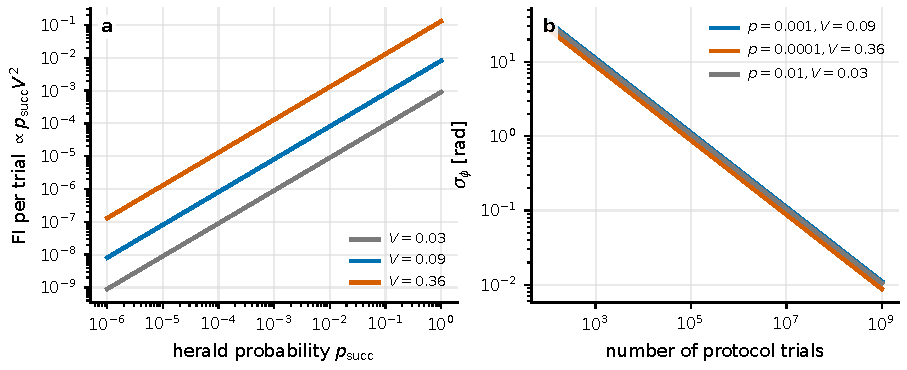
\includegraphics[width=0.94\linewidth]{figures/generated/chapter_17/ch17_fisher_visibility.pdf}
\caption{The statistical payoff of nonlocal phase measurement depends jointly on the success probability and the visibility. The left panel plots the single-trial Fisher-information scale \(p_{\rm succ}V^2\): a threefold drop in visibility gives a ninefold drop in information. The right panel converts the number of trials into phase error, showing that a high repetition rate, a low false-heralding rate, and a high entanglement fidelity must all hold \emph{simultaneously} before anything useful can be claimed.}
\label{fig:e24-fisher-visibility}
\end{figure}

The two-photon precision-astrometry experiment of Crawford et al.\ provides another near-term rung: using two pseudothermal light sources and time-tagging detectors, they observed in a tabletop mock-up the correlation behavior of photon-pair coincidences varying with phase. This experiment is not a complete quantum-network telescope, but it is very well suited as a \emph{rehearsal before going to sky}: time tagging, polarization matching, coherence time, HBT-peak fitting, phase stabilization, and data selection are all directly relevant to real astronomical faint-light observation \citep{2023OExpr..3144246C}.

Placing all the resources on one figure lets us see where we stand: near-term experiments sit roughly in the corner of \(R_{\rm ent}\sim1\)--\(10\,\mathrm{Hz}\), short baselines, and low effective visibility; whereas an astronomically usable ``storage-assisted narrowband'' scheme may need \(R_{\rm ent}\sim\mathrm{kHz}\) to \(100\,\mathrm{kHz}\), \(T_{\rm mem}\sim\mathrm{ms}\) to \(\mathrm{s}\), tens of storage qubits, and very high mode matching; broadband imaging is harder still. The four constraints must close \emph{together}: insufficient \(R_{\rm ent}\) wastes starlight events, insufficient \(T_{\rm mem}\) lets the parity check fall behind, insufficient \(F_{\rm eff}\) washes out the visibility, and if \(R_\star\) is once misestimated, the whole scheme may lose feasibility before the first night of observation.

\begin{figure}[tbp]
\centering
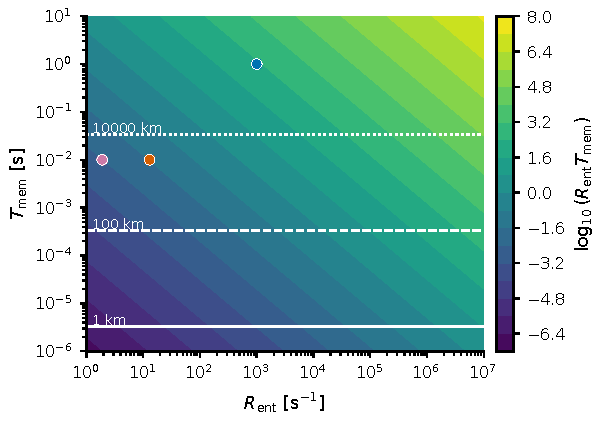
\includegraphics[width=0.94\linewidth]{figures/generated/chapter_17/ch17_network_parameter_space.pdf}
\caption{The resource space of the quantum-network telescope, spanned jointly by the entanglement rate and the storage time. White lines mark the \(B/c\) times corresponding to \(1\,\mathrm{km}\), \(100\,\mathrm{km}\), and \(10^4\,\mathrm{km}\) baselines; the scatter points give the order-of-magnitude gap between the Hz-level entanglement rates of current experiments and the far-term kHz--s-level targets. The color is only the scale of the resource product; full feasibility must be further multiplied by fidelity, mode matching, and the astronomical photon rate.}
\label{fig:e24-network-space}
\end{figure}

\section{How quantum networks and intensity interferometry complement each other}
\label{sec:e24-complementarity}

Please do not write the quantum-network telescope as something that ``replaces intensity interferometry'': it is a \emph{long-term complementary} route. Recall the division of labor between the two: the intensity interferometry of Chapter \ref{chap:e10}, relying on local time tagging plus offline correlation, long ago sidestepped optical-phase transport and is almost immune to atmospheric jitter, at the price of obtaining mainly \(|V|^2\) and losing the phase; the quantum-network route wants to \emph{preserve} the phase of first-order coherence, at the price of paying the whole ledger of entanglement, storage, frequency conversion, and heralding. In the near term, both must develop in parallel with the ELT, VLTI, CHARA, CTAO, and intensity-interferometry arrays.

A pragmatic phased roadmap goes as follows. The \emph{near-term} goal is intensity interferometry and two-photon correlation: the hardware is nearly off-the-shelf (large-area light collectors, SNSPD/SPAD time tagging, narrowband filtering, offline correlation), and the science goals center on the angular diameters of bright stars, binaries, and emission-line regions. The \emph{mid-term} adds local spatial-mode sorting, two-photon astrometry, and GJC-type short-baseline in-sky demonstrations, aiming to prove that the starlight mode can interfere \emph{stably} with a laboratory entanglement resource. Only in the \emph{far term} comes storage-assisted nonlocal first-order-coherence measurement, which requires quantum memory, frequency conversion, entanglement distribution, entanglement fidelity, and astronomical instrumentation to mature synchronously together \citep{1956Natur.178.1046H,2023OExpr..3144246C,2024SPIE13095E..1NR,2026Natur.651..326S}.

\Needspace{11\baselineskip}
Observation planning can start from a concise closure condition:

\begin{equation}
  N_{\rm useful}
  =
  R_\star\,T_{\rm obs}\,
  p_{\rm ready}\,p_{\rm succ}\,V_{\rm meas}^2
  \gtrsim
  N_{\rm req}(\sigma_\theta,\bm{B},\lambda) .
  \label{eq:e24-useful-events}
\end{equation}
\begin{formulaexplain}
\(N_{\rm useful}\) is the number of effective events that actually carry phase information, equal to the product of the starlight event rate, the observation time, the resource-ready probability, the success rate, and the visibility squared; \(N_{\rm req}\) is the number of events needed to reach the target angular precision \(\sigma_\theta\). Only when \(N_{\rm useful}\ge N_{\rm req}\) does the scheme have observational meaning.
\end{formulaexplain}

Naming the terms: \(T_{\rm obs}\) is the total observation time (s), and \(N_{\rm req}\) is set by the target angular precision, the array geometry, and the dimensionality of the model parameters. This equation puts astronomy and quantum engineering into \emph{one ledger}: a bright, narrowband signal with a known arrival time or period lowers the resource pressure, whereas a faint, broadband continuous source amplifies all the difficulties together. It is worth emphasizing that the same ledger applies to more general observation design as well, merely replacing the observable ``nonlocal phase'' with \(|V|^2\), \(g^{(2)}\), polarization angle, or time delay.

So the most valuable product of the quantum-network telescope for now is \emph{not} some already-built instrument but precisely this feasibility ledger that can be checked line by line. In the next chapter we return to the main line of observation design: mapping science goals onto event rates, channels, baselines, backgrounds, and covariances, and only then discussing the trade-offs among intensity interferometry, polarization event tables, transient triggers, and future nonlocal phase measurement.

\section*{Chapter Summary}
\addcontentsline{toc}{section}{Chapter Summary}

\begin{itemize}
\item \textbf{The source of the bottleneck.} Long-baseline amplitude interferometry must send scarce single starlight photons to the same beamsplitter, but the link loss rises \emph{exponentially} with distance (Eq.\ \eqref{eq:e24-link-loss}), while the longer the baseline the higher the resolution (Eq.\ \eqref{eq:e24-resolution-scale}): the allure and the difficulty come from the same dimension.
\item \textbf{Replace what must be transported.} Gottesman--Jennewein--Croke use a known, verifiable, remakeable pre-shared entangled photon \eqref{eq:e24-lab-entangled-photon} in place of hauling starlight over long distances; scanning the local phase \(\delta\) reads the complex visibility \(V\) from the coincidence click rate \eqref{eq:e24-gjc-probability}. The linear-optics Bell measurement incurs about a \(50\%\) event loss.
\item \textbf{The sparsity of faint light is a friend.} Each window contains on average only \(\epsilon\ll1\) starlight photons, so binary time-bin encoding compresses the resource from \(M\sim1/\epsilon\) entangled pairs down to about \(\log_2 M\) storage qubits (Eq.\ \eqref{eq:e24-binary-timebin}), and quantum repeaters and quantum memory take charge of aligning the probabilistically successful events.
\item \textbf{Four items must close together.} The entanglement-supply rate \eqref{eq:e24-entanglement-rate}, the storage time \eqref{eq:e24-memory-time}, the effective fidelity \eqref{eq:e24-effective-fidelity}, and the effective starlight event rate must all meet their targets simultaneously; the fidelity is a \emph{product} of factors, and any one falling short washes out the visibility multiplicatively. The mode mismatch of frequency conversion is especially deadly.
\item \textbf{Two more complementary routes.} Continuous-variable teleportation uses the two-mode squeezed vacuum \eqref{eq:e24-tmsv} to sidestep the \(50\%\) ceiling but with more delicate resources; the ancilla single-photon route \eqref{eq:e24-angle-fisher} lets a remakeable ground photon bear the link risk, but its payoff is sensitive to \(\epsilon\) and to mode indistinguishability.
\item \textbf{Visibility enters the information as a square.} The phase Fisher information of an experiment scales as \(p_{\rm succ}V_{\rm meas}^2\) (Eq.\ \eqref{eq:e24-fisher-visibility}); blindly cranking up the light intensity introduces multiphoton contamination and lowers \(V_{\rm meas}\), instead reducing the total information; quantum networks and intensity interferometry should proceed in phased parallel and complement each other over the long term (Eq.\ \eqref{eq:e24-useful-events}).
\end{itemize}

\medskip
\noindent\textbf{Questions to Ponder.}
\begin{enumerate}
\item If the observing bandwidth \(\Delta\nu\) is narrowed from \(10\,\mathrm{GHz}\) to \(1\,\mathrm{MHz}\), how do the number of entangled photons per second the direct GJC route must prepare, and the number of storage qubits the binary time-bin scheme requires, each change? Why is ``narrowband'' actually favorable for the storage-assisted scheme?
\item In the effective fidelity \eqref{eq:e24-effective-fidelity}, if you could improve only one factor, which would you attack first? Improving \(T/T_2\), the read/write efficiency, and the frequency-conversion efficiency each by \(10\%\), how much improvement does each bring to \(F_{\rm eff}\)?
\item Why does ``raising the heralding success rate \(p_{\rm succ}\)'' not necessarily raise the total Fisher information \(\mathcal I_\phi\)? Use Eqs.\ \eqref{eq:e24-fisher-visibility} and \eqref{eq:e24-psucc} to explain under what conditions multiphoton contamination reverses the payoff.
\end{enumerate}

\chapter{First-Generation Quantum-Astronomy Science Cases}
\label{chap:e25}

\begin{chapteropening}
Over the previous parts we assembled our tools one by one, like gathering gear: complex amplitude and phase (Chapter \ref{chap:e01}), bandwidth and coherence time (Chapter \ref{chap:e02}), Poisson and shot noise (Chapter \ref{chap:e03}), second-order coherence \(g^{(2)}\) and the Siegert relation (Chapter \ref{chap:e08}), intensity interferometry and the van Cittert--Zernike theorem (Chapter \ref{chap:e10}), from visibility to imaging (Chapter \ref{chap:e11}), quantum estimation and SPADE (Chapter \ref{chap:e12}), event tables and clocks (Chapter \ref{chap:e13}), error budgets (Chapter \ref{chap:e15}), all the way to treating the star as a quantum light source (Chapter \ref{chap:e17}) and stitching transients into multi-messenger events (Chapter \ref{chap:e20}). With the gear ready, it is time to take the field. This chapter answers a very practical question: \textbf{under today's instrumental conditions, which pieces of ``doable right now'' real science can first-generation quantum astronomy actually do?} We walk down a checklist (bright-star angular diameters, the flattened spheroids of rapid rotators, close binaries, Be-star disks and Wolf--Rayet winds, the expansion of novae and Type Ia supernovae, the photon statistics of the Crab, natural-laser candidates), and at each stop we ask the same three things: \textbf{which observable do we measure? What array, exposure, and precision are needed? Which astrophysical question does it answer?} This is not pie in the sky but the mapping of every formula from the previous chapters onto targets you could point at tomorrow night.
\end{chapteropening}

\section{Ranking the cases: three yardsticks: brightness, angular scale, external priors}
\label{sec:e25-triage}

You cannot fight a battle by charging in all at once. What a first-generation project fears most is not ``the topic is not pretty enough'' but ``a pretty topic that yields no result.'' So before picking targets, one must establish a cool-headed ranking method, letting scientific value, technical feasibility, and residual product-after-failure all enter the judgment at once.

\textbf{The first yardstick is brightness.} The signal of intensity interferometry is the coincidence count, and its statistical precision is ultimately set by the \textbf{number of photon pairs} accumulated (Chapter \ref{chap:e15}). The higher the photon rate, the more pairs gathered in the same time, and the error falls as the square root of the pair count. For the present generation of instruments, a rough zoning is: hot stars with visual magnitude \(m_V\lesssim5\) are the ``verification zone,'' with strong signals that can be reproduced repeatedly; \(m_V\simeq6\text{--}7\) is the ``challenging but plannable'' zone; and \(m_V\gtrsim9\) usually requires larger arrays, multiple spectral channels, longer integration, or lower system noise to reach. The estimate of LeBohec and Holder gives a memorable anchor: a pair of \(100\,\mathrm{m^2}\) telescopes with electronic bandwidth at the GHz level can, within 5 hours, achieve a several-sigma correlation detection on a source of \(m_V\simeq6.7\) \citep{2006ApJ...649..399L,2013APh....43..331D}.

\textbf{The second yardstick is angular scale.} Brightness decides ``whether there are photons''; angular scale decides ``whether these photons can become parameters.'' As Chapter \ref{chap:e11} explained, an interferometer with baseline \(B\) and wavelength \(\lambda\) can resolve angular scales down to \(\lambda/B\). If the target angular scale \(\theta\gg\lambda/B\), then on long baselines the squared visibility \(|V|^2\) has already fallen nearly to zero, and only short baselines retain signal; if \(\theta\ll\lambda/B\), then all baselines see an ``unresolved point,'' the derivative of the visibility with respect to diameter is nearly zero, and measuring it constrains the parameters hardly at all. Both extremes are bad; the most comfortable case is to have the main structure fall right within the range of baselines you have: \(50\text{--}300\,\mathrm{m}\) for existing IACT arrays, and \(0.5\text{--}2\,\mathrm{km}\) for future CTA-type arrays.

\textbf{The third yardstick is external priors.} The same few \(|V|^2\) data points, if you know in advance the distance, spectrum, orbit, radial velocity, or a theoretical atmosphere model, can be ``translated'' into real physical parameters; if you have no prior at all, a few isolated visibility points are often mutually degenerate, and none can pin down another. So targets with mature priors naturally rank ahead \citep{2003RPPh...66..789M,2012MNRAS.419..172N}.

Writing these three yardsticks into a scorable ranking expression yields a practical triage tool:
\begin{equation}
  \mathcal P
  =
  \frac{
  W_{\rm sci}\,
  R_{\rm tech}\,
  R_{\rm prior}
  }{
  1+R_{\rm sys}+R_{\rm trigger}
  } .
  \label{eq:e25-priority-score}
\end{equation}
\begin{formulaexplain}
\(\mathcal P\) is the project ranking score. In the numerator, the higher the science return \(W_{\rm sci}\), the technical maturity \(R_{\rm tech}\), and the external prior \(R_{\rm prior}\), the higher the score; in the denominator, the higher the systematic-error risk \(R_{\rm sys}\) and the trigger/scheduling risk \(R_{\rm trigger}\), the lower the score. It is designed specifically to prevent starting a project ``just because the topic sounds nice.''
\end{formulaexplain}
Grounding each term: \(W_{\rm sci}\) is the science return (how important this result is), \(R_{\rm tech}\) is the technical maturity (whether existing instruments can stably deliver it), \(R_{\rm prior}\) is the external prior and model interpretability, \(R_{\rm sys}\) is the systematic-error risk (how easily zero-baseline correlation, time synchronization, and background subtraction go wrong), and \(R_{\rm trigger}\) is the trigger and scheduling risk (whether one must compete for a time window, and whether one can start up at any time). These quantities are all dimensionless; in practice one need only grade them coarsely (high/medium/low), the aim being not to compute a precise decimal but to \textbf{prevent any single dimension from dominating the choice}. A comparison: the geometric distance of Type Ia has extremely high \(W_{\rm sci}\), but its \(R_{\rm trigger}\) and \(R_{\rm sys}\) are also high, propping up the denominator, so the first generation should not force it; the angular diameter of bright stars has only moderate \(W_{\rm sci}\), yet very high \(R_{\rm tech}\) and very low system risk, so its score is instead steady, making it especially suitable as one of the first batch of ``acceptance metrics'' \citep{2024ApJ...966...28A,2024MNRAS.529.4387A,2025PhRvD.111h3047K}.

\begin{figure}[tbp]
\centering
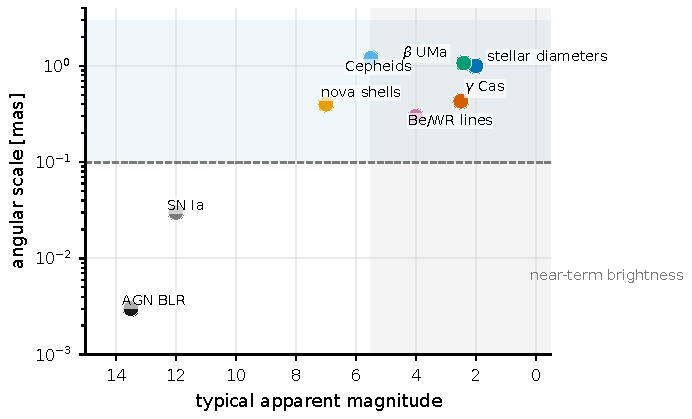
\includegraphics[width=0.88\linewidth]{figures/generated/chapter_19/ch19_science_case_feasibility.pdf}
\caption{The positions of first-generation candidate targets on the ``brightness--angular scale'' plane. Bright-star angular diameters, \(\beta\) UMa, \(\gamma\) Cas, and the Be/WR spectral-line regions simultaneously satisfy ``bright enough'' and ``resolvable by hundred-meter baselines,'' falling in the most comfortable region; Type Ia, AGN broad-line regions, and dark-matter small-scale lensing have very high scientific value, yet are pushed toward long-term projects by brightness, event rate, or angular scale. This figure is the visualization of the three yardsticks in Eq.\ \eqref{eq:e25-priority-score}.}
\label{fig:e25-case-plane}
\end{figure}

With this ranking in hand, the order of the rest of this chapter is in fact already implicit: first do the targets that fall in the upper-right ``comfortable region'' of Figure \ref{fig:e25-case-plane}, then step by step push toward directions of higher scientific value but also higher risk.

\section{Stellar angular diameter and effective temperature: the most mature first-generation product}
\label{sec:e25-diameter}

Why is the first task to measure a star's \textbf{angular diameter}? Because it simultaneously satisfies the three yardsticks above, and its output is direct, reproducible, and can serve repeatedly as an acceptance standard. The observable is very clean: measure the squared visibility \(|V|^2(B,\lambda)\) over a range of baselines \(B\) and wavelengths \(\lambda\), and the model begins from the simplest \textbf{uniform disk}, then corrects with a \textbf{limb-darkening} (the disk's edge is dimmer than its center) profile or a full atmosphere model.

The most elegant use of angular diameter is that it directly pins down a star's \textbf{effective temperature}. Not a single step in this chain of logic can be skipped, so we lay it out. A star of radius \(R\) and effective temperature \(T_{\rm eff}\) has luminosity given by the Stefan--Boltzmann law, \(L=4\pi R^2\sigma_{\rm SB}T_{\rm eff}^4\). These photons travel to the Earth at distance \(D\), spread over a sphere of radius \(D\), so the \textbf{bolometric flux} we receive is
\[
  F_{\rm bol}=\frac{L}{4\pi D^2}
  =\frac{R^2}{D^2}\,\sigma_{\rm SB}T_{\rm eff}^4
  =\left(\frac{R}{D}\right)^2\sigma_{\rm SB}T_{\rm eff}^4 .
\]
Note that \(R/D\) is precisely the star's \textbf{angular radius}, and the angular diameter \(\theta_{\rm LD}=2R/D\), so \(R/D=\theta_{\rm LD}/2\) and \((R/D)^2=\theta_{\rm LD}^2/4\). Substituting back gives the central equation of this section:
\begin{equation}
  F_{\rm bol}
  =
  \frac{\theta_{\rm LD}^2}{4}
  \sigma_{\rm SB}T_{\rm eff}^4,
  \qquad
  T_{\rm eff}
  =
  \left(
  \frac{4F_{\rm bol}}
  {\sigma_{\rm SB}\theta_{\rm LD}^2}
  \right)^{1/4}.
  \label{eq:e25-teff}
\end{equation}
\begin{formulaexplain}
\(F_{\rm bol}\) is the bolometric flux received at Earth, \(\theta_{\rm LD}\) is the limb-darkened angular diameter, \(\sigma_{\rm SB}\) is the Stefan--Boltzmann constant, and \(T_{\rm eff}\) is the effective temperature. In a word: once the angular diameter is measured accurately, ``flux'' can be directly converted into the star's ``temperature scale.''
\end{formulaexplain}
Accounting for units and dimensions one by one: \(F_{\rm bol}\) has units \(\mathrm{erg\,s^{-1}\,cm^{-2}}\), obtained by integrating multiband photometry; \(\theta_{\rm LD}\) has units of rad (the milliarcsecond, mas, is a common practical unit, with \(1\,\mathrm{mas}=4.85\times10^{-9}\,\mathrm{rad}\)); \(\sigma_{\rm SB}=5.67\times10^{-5}\,\mathrm{erg\,s^{-1}\,cm^{-2}\,K^{-4}}\); and \(T_{\rm eff}\) has units of K. The beauty of this equation is that it is \textbf{independent of distance}: both \(F_{\rm bol}\) and \(\theta_{\rm LD}\) are directly observable, and the intervening \(D\) has already canceled out in the derivation.

How does the error in angular diameter propagate to the temperature? Take the logarithmic differential of \(T_{\rm eff}\) with respect to \(\theta_{\rm LD}\). Because \(T_{\rm eff}\propto\theta_{\rm LD}^{-1/2}\) (treating \(F_{\rm bol}\) as an independent measurement), we have
\[
  \ln T_{\rm eff}=\text{const}-\tfrac12\ln\theta_{\rm LD}
  \;\Longrightarrow\;
  \frac{\delta T_{\rm eff}}{T_{\rm eff}}=-\frac12\frac{\delta\theta_{\rm LD}}{\theta_{\rm LD}} .
\]
So a \(4\%\) error in angular diameter, propagated by this path alone, becomes only \(2\%\) in temperature. This ``halving'' relation explains why bright-star angular diameters are worth measuring again and again: it is not a one-off instrumental flourish but \textbf{foundational data} that flows into \(T_{\rm eff}\), stellar radius, age, rotation models, and the standard-star scale \citep{1967MNRAS.137..393H,1977MNRAS.180..177B,2003RPPh...66..789M}.

This route has traveled from history into the present. Last century the Narrabri intensity interferometer measured the diameters of a batch of bright stars using the method of Hanbury Brown and Twiss \citep{1956Natur.178.1046H,1974MNRAS.167..121H}; today VERITAS's intensity-interferometry system (VERITAS-SII) has advanced it to sub-milliarcsecond precision, giving diameters for \(\beta\) CMa and \(\epsilon\) Ori, and achieving better than \(5\%\) with far less observing time than in the old days; a subsequent measurement of \(\beta\) UMa at 416 nm gave a limb-darkened angular diameter \(\theta_{\rm LD}=1.07\pm0.04_{\rm stat}\pm0.05_{\rm sys}\,\mathrm{mas}\), cross-checked against CHARA near-infrared and Keck mid-infrared results. MAGIC's upgraded system (MAGIC-SII) reported 22 stellar diameters in one go, 13 of them with no prior comparable measurement: intensity interferometry has gone from ``a single demonstration'' to ``producing data in batches'' \citep{2020NatAs...4.1164A,2024ApJ...966...28A,2024MNRAS.529.4387A}. One point to note here is that these results use \textbf{second-order} coherence (Chapters \ref{chap:e08}, \ref{chap:e10}), which is insensitive to atmospheric seeing and optical-path phase, and this is precisely why it can still work on narrowband, ultra-long baselines.

\textbf{What is needed, what is answered?} The array this case needs is very plain: a few pairs of off-the-shelf IACT telescopes, hundred-meter baselines, narrowband filtering, GHz-level electronic bandwidth, and integration from a few hours to a few nights; the precision goal is to measure the diameter to \(3\text{--}5\%\), reproducible over multiple nights. It answers the most basic question in stellar physics, \textbf{just how big and how hot this star really is}, and thereby calibrates the entire scale of stellar parameters and distances.

\section{Rapid rotation: upgrading from ``how big'' to ``what shape''}
\label{sec:e25-rotation}

Measuring the diameter is only the first step. Many hot stars rotate so fast that centrifugal force flings the equator into a bulge, and the photosphere becomes a flattened ellipsoid; moreover, by the von Zeipel theorem, the bulging equator has weaker gravity, lower temperature, and is dimmer, while the poles are brighter and hotter; this is \textbf{gravity darkening}. To see such structure, the uniform-disk model no longer suffices: it has only one parameter \(\theta\), whereas a flattened ellipsoid needs at least three: the minor-axis angular diameter \(\theta_{\rm min}\), the \textbf{axial ratio} \(r=\theta_{\rm maj}/\theta_{\rm min}\), and the position angle \(\varphi_\star\).

How do we write this flattened sphere as a fittable visibility curve? First recall the known result of Chapter \ref{chap:e11}: a uniform disk of angular diameter \(\theta\) has first-order visibility modulus of Airy form \(|V|=|2J_1(x)/x|\), where \(x=\pi B\theta/\lambda\) is the dimensionless spatial frequency and \(J_1\) is the first-order Bessel function (the standard result for circular-aperture diffraction, with its first zero at argument \(3.83\)). The trick for the ellipsoid is that the ``effective diameter'' seen along different projection directions differs: seen along the minor axis it is \(\theta_{\rm min}\), and seen along the major axis it is \(r\theta_{\rm min}\). Folding this directional dependence into \(x\) gives
\begin{equation}
  x_{\rm ell}
  =
  \frac{\pi B_p\theta_{\rm min}}{\lambda}
  \left[
  \cos^2\psi
  +
  r^2\sin^2\psi
  \right]^{1/2},
  \qquad
  |V_{\rm ell}|^2
  =
  \left[\frac{2J_1(x_{\rm ell})}{x_{\rm ell}}\right]^2 .
  \label{eq:e25-elliptical-visibility}
\end{equation}
\begin{formulaexplain}
\(x_{\rm ell}\) is the dimensionless spatial frequency of the flattened ellipsoid on the current projected baseline, \(B_p\) is the projected baseline length, \(\psi\) is the direction angle of the projected baseline relative to the minor axis, and \(r\) is the axial ratio. The factor in the brackets folds ``the direction of viewing'' into the effective diameter: along the minor axis (\(\psi=0\)) it reduces to \(\theta_{\rm min}\), and along the major axis (\(\psi=90^\circ\)) it becomes \(r\theta_{\rm min}\).
\end{formulaexplain}
Check the bracket once and its geometry is clear: when \(\psi=0\) (baseline aligned with the minor axis), \(\cos^2\psi=1,\sin^2\psi=0\), so \(x_{\rm ell}=\pi B_p\theta_{\rm min}/\lambda\), and one sees the minor axis; when \(\psi=90^\circ\), \(x_{\rm ell}=\pi B_p(r\theta_{\rm min})/\lambda\), and one sees the major axis. Grounding the parameters: hot-star axial ratios are typically \(r\simeq1.1\text{--}1.5\), with minor-axis angular diameters often below \(1\,\mathrm{mas}\). Here is a key \textbf{observation-design} lesson: to pin down both \(r\) and \(\varphi_\star\) at once, you must obtain \(|V|^2\) at \textbf{multiple position angles}: single-direction baseline coverage badly degenerates \(r\) and \(\varphi_\star\), because one curve can be jointly fit by ``more flattened but rotated'' and ``less flattened.'' This is precisely the language of uv coverage from Chapter \ref{chap:e11} cashed out on a concrete target.

In reality this has already been done. VERITAS's observation of the classic rapid rotator \(\gamma\) Cas gave a minor-axis angular diameter of about \(0.43\pm0.02_{\rm stat}\pm0.02_{\rm sys}\,\mathrm{mas}\), an axial ratio of about \(1.28\pm0.04\pm0.02\), and a rotation-axis position angle of about \(116^\circ\), and inferred with a Roche--von Zeipel model that it is already near \textbf{critical (breakup) rotation}, where the equatorial centrifugal force nearly balances gravity \citep{2025ApJ...995..191A}. This means first-generation intensity interferometry can already advance from ``how big is this star'' to ``what shape is this star, and how much do the poles and equator differ in temperature.''

\textbf{What is needed, what is answered?} This case needs coverage of \textbf{two or more distinctly different position angles} on the same target, with all other requirements the same as for angular diameter; the precision goal is to statistically distinguish the disk model from the ellipse model. It answers a deep question in stellar structure and evolution: \textbf{how rotation alters a star's shape, temperature distribution, and even lifetime}.

\section{Binaries, Be-star disks, and Wolf--Rayet winds: separating them with the baseline}
\label{sec:e25-binary}

Intensity interferometry can measure not only ``how big a source is'' but also see through ``it is actually two sources.'' The advantage of a \textbf{close binary} is that its signal has an extremely high recognizability. Consider two unresolved point sources with angular separation vector \(\bm s\) and \textbf{flux ratio} \(f=F_2/F_1\). Their combined coherence function is the superposition of the individual complex amplitudes weighted by flux; after normalization it is \((1+f\,e^{-2\pi i\,\bm u\cdot\bm s})/(1+f)\), where \(\bm u=\bm B_\perp/\lambda\) is the spatial frequency. The squared visibility is its modulus squared, and we expand this step without skipping any:
\[
  |V_{\rm binary}|^2
  =\frac{|1+f e^{-i\phi}|^2}{(1+f)^2},
  \qquad \phi\equiv 2\pi\,\bm u\cdot\bm s .
\]
Using \(|1+f e^{-i\phi}|^2=(1+f\cos\phi)^2+(f\sin\phi)^2=1+2f\cos\phi+f^2\cos^2\phi+f^2\sin^2\phi=1+f^2+2f\cos\phi\) (using only \(\cos^2+\sin^2=1\)), we obtain
\begin{equation}
  |V_{\rm binary}|^2
  =
  \frac{1+f^2+2f\cos(2\pi\,\bm u\cdot\bm s)}
  {(1+f)^2}.
  \label{eq:e25-binary-visibility}
\end{equation}
\begin{formulaexplain}
\(\bm u=\bm B_\perp/\lambda\) is the spatial frequency, \(\bm s\) is the binary angular-separation vector, and \(f\) is the flux ratio. The phase in the exponent varies with the baseline, making \(|V|^2\) \textbf{oscillate} along the baseline: it is precisely this oscillating curve that lets intensity interferometry constrain the separation and orientation of the binary.
\end{formulaexplain}
The key to reading this equation is the \textbf{amplitude} of that cosine term, \(2f/(1+f)^2\). When \(f=1\) (equal-brightness binary), \(|V|^2\) oscillates all the way from \(1\) (at \(\cos=+1\)) to \(0\) (at \(\cos=-1\)), a deep and easily recognizable signal; when \(f=0.1\) (a faint companion only one-tenth as bright as the primary), the half-amplitude of the cosine term is only \(2(0.1)/(1.1)^2\simeq0.17\), and \(|V|^2\) swings by this half-amplitude about its mean \((1+f^2)/(1+f)^2=1.01/1.21\simeq0.83\), that is, it ripples from a trough of \((1-f)^2/(1+f)^2=(0.9/1.1)^2\simeq0.67\) to a peak of \(1.0\), a modulation depth of only about \(0.33\), sharply raising the demands on signal-to-noise and calibration. The \textbf{period} of the oscillation is set by the separation \(\bm s\): the larger the separation, the faster \(|V|^2\) oscillates with baseline. So binary projects are best suited to systems that \textbf{already have spectroscopic-orbit or eclipsing-binary priors}: each night one need only obtain a few baseline points to be threaded onto a known orbit model; even if a given night fails, one can still give an upper limit on the separation or brightness ratio, so the night is not a total loss \citep{1974MNRAS.167..121H,2012MNRAS.419..172N,2014MNRAS.437..798M,2022MNRAS.512.1722K}.

\begin{figure}[tbp]
\centering
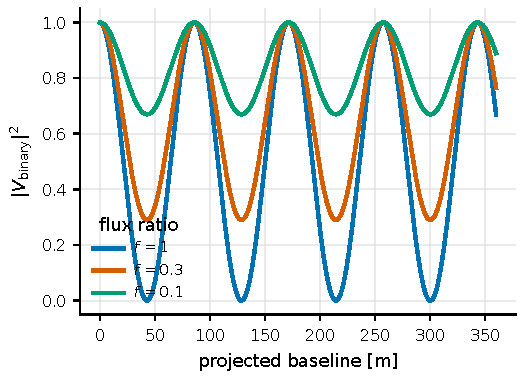
\includegraphics[width=0.82\linewidth]{figures/generated/chapter_19/ch19_binary_visibility.pdf}
\caption{The squared-visibility oscillation of a \(1\,\mathrm{mas}\) binary at 416 nm. An equal-brightness binary (\(f=1\)) gives a deep oscillation from 1 to 0; as the flux ratio drops to \(0.3\) then \(0.1\), it rapidly shallows following the amplitude \(2f/(1+f)^2\) of Eq.\ \eqref{eq:e25-binary-visibility}. Binary projects therefore depend especially on multi-position-angle baseline coverage and known orbital priors; otherwise the brightness ratio, separation, and position angle become mutually degenerate.}
\label{fig:e25-binary-visibility}
\end{figure}

One step further is to combine ``spatial resolution'' with ``spectral-line selection'' to dissect \textbf{Be-star decretion disks} (equatorial gas disks thrown off by rapidly rotating B-type stars) and \textbf{Wolf--Rayet winds} (high-speed stellar winds of massive stars). The continuum of these sources comes mainly from the photosphere, while emission lines such as \(\mathrm{H}\alpha\), He, and Fe come from a larger, more extended disk or wind-collision region. The trouble is that within a single filter the \textbf{line and continuum are often mixed}, and the measured visibility is a flux-weighted average of the two:
\begin{equation}
  V_{\rm obs}
  =
  \frac{
  F_{\rm c}V_{\rm c}
  +
  F_{\rm line}V_{\rm line}
  }{
  F_{\rm c}+F_{\rm line}
  } .
  \label{eq:e25-line-continuum}
\end{equation}
\begin{formulaexplain}
\(V_{\rm c},V_{\rm line}\) are respectively the visibilities of the continuum region and the line region, and \(F_{\rm c},F_{\rm line}\) are the corresponding fluxes. The \(V_{\rm obs}\) you measure is a flux-weighted average of the two, so the line geometry must first be ``subtracted'' from the continuum before it can be interpreted on its own.
\end{formulaexplain}
Here \(F_{\rm line}/F_{\rm c}\) can be estimated from simultaneous spectroscopy or a ``narrowband-minus-continuum'' dual-filter measurement. The physical reading is intuitive: if the line region is \textbf{larger} than the photosphere (as for an extended disk), then \(V_{\rm line}\) falls faster than the continuum on long baselines, and the mixed \(V_{\rm obs}\) is pulled down by the line at the long-baseline end; conversely, if the line comes from a very small, high-brightness spot, it instead retains signal on long baselines. Historically the Narrabri measurement of the Wolf--Rayet binary \(\gamma^2\) Velorum already showed that the emission-line region and the continuum region can have \textbf{different angular scales} \citep{1970MNRAS.148..103H,2010SPIE.7734E..0AD,2012NewAR..56..143D,2025ApJ...995..191A}. Modern multi-baseline arrays can generalize this idea to the geometry of Be-star disks, the line profiles of rapidly rotating hot stars, and the wind-collision regions of interacting binaries.

\textbf{What is needed, what is answered?} This case needs narrowband filtering or simultaneous spectroscopy to separate line from continuum, a verifiable continuum subtraction, and sufficient line flux; it answers questions like \textbf{how a star ejects matter, and what geometry the disk and wind take}, questions hard to image directly by other means.

\section{Expanding transients: novae are doable now, Type Ia is a long-term goal}
\label{sec:e25-transient}

Now turn the lens to sources that ``grow.'' Novae and supernovae eject an expanding shell whose geometric ledger is extremely simple: if the shell expands approximately freely at velocity \(v_{\rm exp}\), then at time \(t-t_0\) after the outburst, the angular diameter it subtends is ``twice the traversed linear radius divided by the distance'':
\begin{equation}
  \theta(t)
  \simeq
  \frac{2v_{\rm exp}(t-t_0)}{D},
  \qquad
  D
  \simeq
  \frac{2v_{\rm exp}(t-t_0)}{\theta}.
  \label{eq:e25-expansion}
\end{equation}
\begin{formulaexplain}
\(\theta(t)\) is the angular diameter of the expanding shell, \(v_{\rm exp}\) is the expansion velocity, \(t_0\) is the outburst time, and \(D\) is the distance. The left equation predicts ``how big the shell is,'' and the right inverts it for ``how far away we are'': this is the \textbf{expansion parallax}, independent of a standard candle.
\end{formulaexplain}
Accounting term by term: \(v_{\rm exp}\) comes from the Doppler velocity of spectral lines (Chapter \ref{chap:e20} explained how to read velocity from wavelength shifts), with units \(\mathrm{cm\,s^{-1}}\); \(t-t_0\) is the time after outburst, with units s; and \(D\) is the distance, with units cm. Its physical premise is a plain statement: \(v_{\rm exp}\) and \(\theta\) must correspond to \textbf{the same layer of matter}, otherwise the distance from the right equation is systematically biased (Chapter \ref{chap:e20} analyzed this trap in detail).

Substituting two sets of real numbers, what the first generation can and cannot do becomes immediately clear. \textbf{Galactic nova}: take \(D=2\,\mathrm{kpc}=6.17\times10^{21}\,\mathrm{cm}\), \(v_{\rm exp}=10^8\,\mathrm{cm\,s^{-1}}\), \(t-t_0=10\,\mathrm{d}=8.64\times10^5\,\mathrm{s}\). The linear radius \(v_{\rm exp}(t-t_0)=8.64\times10^{13}\,\mathrm{cm}\), and the angular diameter \(\theta=\dfrac{2\times8.64\times10^{13}}{6.17\times10^{21}}=2.80\times10^{-8}\,\mathrm{rad}\). Converting with \(1\,\mathrm{rad}=2.063\times10^8\,\mathrm{mas}\), \(\theta\approx5.8\,\mathrm{mas}\), within ten days it reaches a few milliarcseconds, resolvable with baselines below one hundred meters. \textbf{Type Ia supernova}: take \(D=10\,\mathrm{Mpc}=3.09\times10^{25}\,\mathrm{cm}\), \(v_{\rm exp}=10^9\,\mathrm{cm\,s^{-1}}\), \(t-t_0=20\,\mathrm{d}=1.73\times10^6\,\mathrm{s}\). The linear radius \(1.73\times10^{15}\,\mathrm{cm}\), and \(\theta=\dfrac{2\times1.73\times10^{15}}{3.09\times10^{25}}=1.12\times10^{-10}\,\mathrm{rad}\approx0.023\,\mathrm{mas}\), even with a velocity ten times higher, twenty days later it is only a few tens of microarcseconds, needing \textbf{kilometer-scale} optical baselines to reach.

\begin{figure}[tbp]
\centering
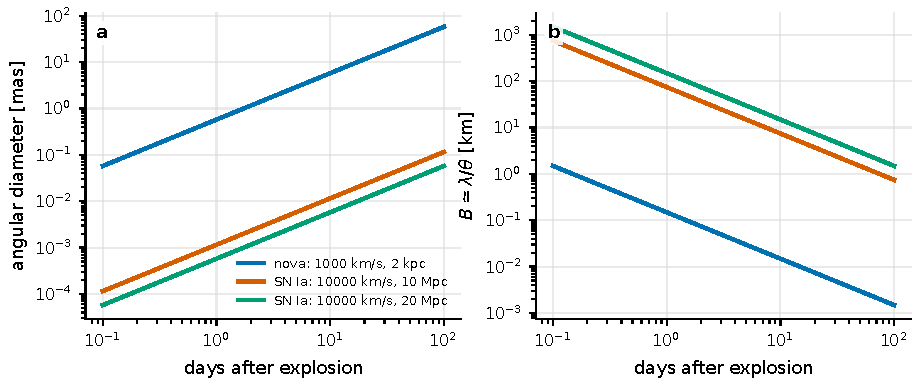
\includegraphics[width=0.94\linewidth]{figures/generated/chapter_19/ch19_transient_expansion.pdf}
\caption{The angular diameter of expanding transients and the required baseline. A Galactic nova enters the milliarcsecond regime within a few days to a few tens of days, well suited for the first generation to rehearse the whole ``trigger--schedule--image'' chain; a Type Ia at \(10\text{--}20\,\mathrm{Mpc}\) is only a few tens of microarcseconds even near peak, requiring kilometer-scale baselines and a nearby event with \(m\lesssim12\). The curves are precisely the behavior of Eq.\ \eqref{eq:e25-expansion} for various \(v_{\rm exp}\) and \(D\).}
\label{fig:e25-transient-expansion}
\end{figure}

So the first generation's division of labor is clear: the \textbf{Galactic nova} is a realistic target, its angular scale large enough and bright enough, best suited for running through the whole pipeline of trigger, filtering, background subtraction, and model fitting, with the main difficulties coming from rapid brightness evolution, non-spherical shell asymmetry, and dust obscuration. The \textbf{geometric distance of Type Ia} is a high-return long-term goal: the feasibility study of Kim et al.\ takes \(m\lesssim12\) (corresponding to a local volume of \(z\sim0.004\), about one per year over the whole sky) as the brightness range foreseeable for the next generation, and uses radiative-transfer models to compute the surface brightness and \(|V|^2\) at various wavelengths, pointing out that \textbf{spectral resolution} can provide multiwavelength tomography, so the measurement is no longer confined to a single uniform-disk radius \citep{2025PhRvD.111h3047K,1997A&A...320..799F,2004A&A...415..531S}. In other words, the Type Ia distance ruler should be slotted into second-generation or dedicated arrays, not into the first generation's acceptance items.

\textbf{What is needed, what is answered?} The nova case needs \textbf{fast triggering} (responding within hours) plus simultaneous line velocities, pairing \(\theta(t)\) with \(v_{\rm exp}\); it answers ``how far away this outburst is, and whether the shell is spherically symmetric,'' and lays technical groundwork for future use of expansion parallax to independently calibrate the cosmic distance ladder.

\section{The Crab and natural lasers: testing ``non-thermal'' with photon statistics}
\label{sec:e25-statistics}

The previous sections all used \textbf{visibility} (the spatial information of second-order coherence). This section switches glasses to \textbf{temporal statistics}: precisely where the event table (Chapter \ref{chap:e13}) and \(g^{(2)}\) (Chapter \ref{chap:e08}) come into their own.

First the \textbf{Crab pulsar}. It is not a good target for spatial intensity interferometry (it is a point source), but it is an excellent object for event-table science: bright, stably periodic, with a precise ephemeris, and an optical main pulse and interpulse that define clear \textbf{phase windows}. The premise for placing each photon into the correct phase window is that the time stamp is accurate enough. The conversion between phase error and time error is a single line:
\begin{equation}
  \Delta\phi
  =
  \frac{\Delta t}{P_{\rm spin}}.
  \label{eq:e25-pulse-phase}
\end{equation}
\begin{formulaexplain}
\(\Delta t\) is the photon time-stamp error, \(P_{\rm spin}\) is the pulsar spin period, and \(\Delta\phi\) is the converted phase error (dimensionless, with \(0\text{--}1\) corresponding to a full period). The more accurate the timing, the better the photon can be placed into the pulse-phase window it truly belongs to.
\end{formulaexplain}
Order of magnitude: the Crab's \(P_{\rm spin}\simeq33\,\mathrm{ms}\), and a \(1\,\mu\mathrm{s}\) timing error corresponds to only \(\Delta\phi\simeq10^{-6}/(33\times10^{-3})\approx3\times10^{-5}\); extremely comfortable, microsecond-level synchronization is ample. But the same equation tells you that a millisecond pulsar (\(P\sim\mathrm{ms}\)), to preserve the same narrow phase structure, must push \(\Delta t\) down to the nanosecond level. With phase windows in hand, one can do what past average light curves could not: phase-resolved \(g^{(2)}\), color correlations, and conditional stacking against radio \textbf{giant pulses}. Instruments like AquEYE/Iqueye can already save photons with picosecond-to-nanosecond time tags; observationally, the optical emission is enhanced in periods with Crab giant radio pulses, and ARCONS also saw that earlier-arriving giant pulses correspond to stronger optical enhancement \citep{2009JMOp...56..261B,2009A&A...508..531N,2015SPIE.9504E..0CZ,2003Sci...301..493S,2013ApJ...779L..12S}. What first-generation quantum astronomy is to do is upgrade these results from ``average light curves'' to ``event-table statistics + polarization/color windowing.''

\begin{figure}[tbp]
\centering
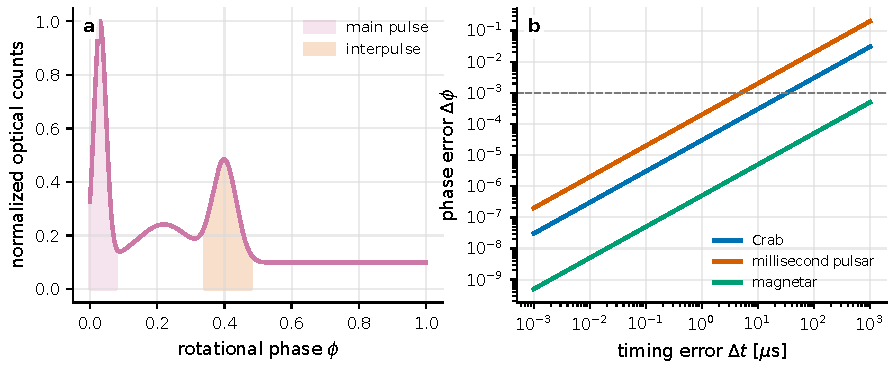
\includegraphics[width=0.94\linewidth]{figures/generated/chapter_19/ch19_crab_phase_windows.pdf}
\caption{The phase windows and time error of Crab-type optical pulses. The left panel sketches the three event-selection windows of main pulse, bridge, and interpulse; the right panel converts the time error into phase error via Eq.\ \eqref{eq:e25-pulse-phase}. For the Crab, microsecond-level timing is more than enough; for millisecond pulsars, ns--\(\mu\mathrm{s}\)-level synchronization is needed to preserve the narrow phase structure.}
\label{fig:e25-crab-phase}
\end{figure}

Next, \textbf{natural-laser} (natural / astrophysical laser) candidates. What these targets test is a very pure quantum question: \textbf{are the photon statistics of this bright spectral line thermal or coherent?} But beware a trap: ``seeing a bright spectral line'' is by itself \textbf{insufficient} to declare a laser, because the superposition of many mutually incoherent thermal modes can also average away the bunching peak. Quantitatively, for \(M\) mutually incoherent thermal modes,
\begin{equation}
  g^{(2)}(0)-1
  =
  \frac{1}{M},
  \label{eq:e25-mode-bunching}
\end{equation}
\begin{formulaexplain}
\(M\) is the number of mutually incoherent thermal modes superposed in the detection, and \(g^{(2)}(0)\) is the zero-delay second-order coherence. Single-mode thermal light has \(g^{(2)}(0)=2\) (bunching), but the larger \(M\), the more the bunching peak is averaged away, and \(g^{(2)}(0)\to1\). So \(g^{(2)}(0)\) close to 1 does not necessarily mean the light is an ideal laser.
\end{formulaexplain}
For comparison, remember the two extremes of Chapter \ref{chap:e08}: single-mode thermal state \(g^{(2)}(0)=2\), and ideal coherent state \(g^{(2)}(0)=1\). Equation \eqref{eq:e25-mode-bunching} says that ``multimode thermal light disguises itself as coherent light,'' so this kind of test must be accompanied by a \textbf{null test}: accounting cleanly for the mode number, the instrument time response, and the continuum background, before one can judge what a deviation of \(g^{(2)}(0)\) from 1, or its proximity to 1, means. Another usable handle is the line width: if the line width is \(\Delta\nu\), the coherence time is about \(\tau_c\sim1/(\pi\Delta\nu)\) (the concrete form of the bandwidth--coherence-time relation of Chapter \ref{chap:e02}). For example, if a natural-laser line is as narrow as \(\Delta\nu\sim1\,\mathrm{GHz}\), then \(\tau_c\sim1/(\pi\times10^9)\approx3\times10^{-10}\,\mathrm{s}=0.3\,\mathrm{ns}\); the narrower the line and the longer the coherence time, the easier it is to preserve a resolvable correlation \textbf{contrast} at a given detector time resolution. Among real candidates, the Fe II lines in the Weigelt blobs of Eta Carinae are pumped by \(\mathrm{Ly}\alpha\), and Johansson and Letokhov discussed Fe II laser lines at \(0.9\text{--}1.0\,\mu\mathrm{m}\) and in the near-infrared; line-width measurement plus photon-correlation spectroscopy can provide direct evidence \citep{2004A&A...428..497J,2005NewA...10..361J,2008AIPC..984..216D}.

\begin{figure}[tbp]
\centering
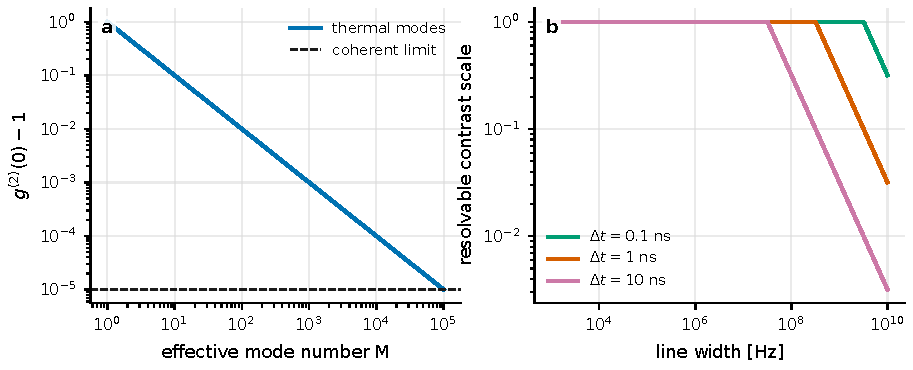
\includegraphics[width=0.94\linewidth]{figures/generated/chapter_19/ch19_natural_laser_statistics.pdf}
\caption{Two statistical criteria for natural-laser candidates. The left panel shows that increasing the number of thermal modes \(M\) lowers the bunching peak per Eq.\ \eqref{eq:e25-mode-bunching}, approaching the coherent limit \(g^{(2)}(0)-1=0\); the right panel shows that the narrower the line and the longer the coherence time, the easier it is to preserve a resolvable contrast at a given time resolution. Together they show: judging ``whether it is a laser'' requires jointly using photon statistics and line width, with a rigorous null test.}
\label{fig:e25-natural-laser}
\end{figure}

\textbf{What is needed, what is answered?} These two classes of case depend more on \textbf{event-table quality}: absolute time synchronization, a precise ephemeris, a verifiable background subtraction, and narrowband selection capable of separating line from continuum; they answer ``what quantum-statistical nature this light has,'' pushing the radiation mechanism (Chapter \ref{chap:e16}) from the spectral level to the photon-statistical level.

\section{Arranging the checklist into a roadmap: the order shifts as the instrument matures}
\label{sec:e25-roadmap}

Placing all the cases above into one matrix, the first generation's order of advance is set mainly by \textbf{technical maturity} and \textbf{system risk}, not purely by scientific value. Figure \ref{fig:e25-priority} is this matrix: the horizontal axis is technical maturity, the vertical axis is science return, and the larger the point, the higher the systematic and trigger risk.

\begin{figure}[!htbp]
\centering
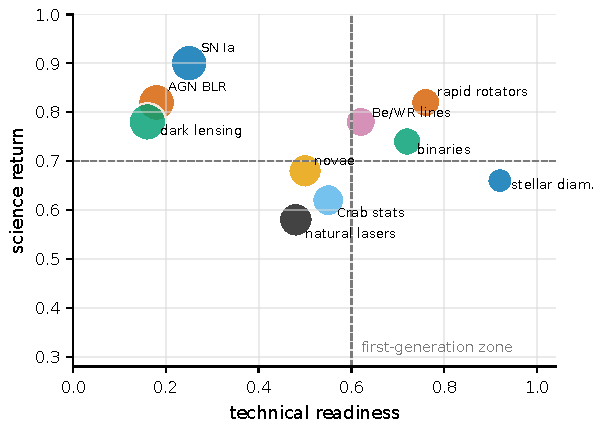
\includegraphics[width=0.78\linewidth]{figures/generated/chapter_19/ch19_priority_matrix.pdf}
\caption{The first-generation science-case matrix. The horizontal axis is technical maturity, the vertical axis is science return, and the larger the point, the higher the systematic-error and trigger risk. Targets in the upper right with smaller points are best suited as first-generation acceptance items; upper-left targets (Type Ia, AGN broad-line regions, dark-matter small-scale lensing) have high scientific value but need dedicated arrays or more mature quantum resources, and belong to the long-term category.}
\label{fig:e25-priority}
\end{figure}

The reading is this: targets in the \textbf{upper right with small points} (angular diameters of bright hot stars, reference stars of known diameter, \(\beta\) UMa-type A stars, MAGIC/VERITAS reproducible targets) are low-risk and reproducible, and naturally the first batch of acceptance projects; adding scientific information on the same capability are \(\gamma\) Cas-type rapid rotators, Be/WR line regions, close binaries, and early nova expansion; more dependent on event-table quality and time/spectral selection are Crab phase-resolved statistics and natural-laser candidate lines; while those high-value upper-left targets, such as Type Ia geometric distance, AGN broad-line regions, dark-matter small-scale lensing, and quantum-network-assisted imaging (Chapter \ref{chap:e24}), should be placed firmly among the long-term goals.

The table below lists side by side the first observable, typical order of magnitude, and ``whether it counts as first-generation'' criterion for the seven classes of case, for easy comparison. It is in fact the ranking of Eq.\ \eqref{eq:e25-priority-score} cashed out into an executable checklist:

\begin{longtable}{p{0.17\linewidth}p{0.22\linewidth}p{0.23\linewidth}p{0.20\linewidth}}
\toprule
Case & First observable & Typical order of magnitude & First-generation criterion \\
\midrule
Bright-star angular diameter & \(|V|^2(B)\) & \(m_V<5\), \(\theta=0.5\text{--}2\,\mathrm{mas}\) & Multi-night repeatable to \(3\text{--}5\%\) diameter precision. \\
Rapid rotation & Multi-position-angle \(|V|^2\) & Axial ratio \(1.1\text{--}1.5\), \(\theta<1\,\mathrm{mas}\) & Can distinguish disk from ellipse model. \\
Binary & \(|V|^2\) oscillation & Separation \(0.2\text{--}5\,\mathrm{mas}\), \(f>0.1\) & Has orbital prior, covers two or more position angles. \\
Be/WR line & Line/continuum \(|V|^2\) & \(\mathrm{H}\alpha\), He, Fe lines & Sufficient line flux, verifiable continuum subtraction. \\
Nova & \(\theta(t)\) & mas level after a few days & Fast trigger, can merge with line velocity. \\
Crab statistics & Phase-window \(g^{(2)}\), color correlation & \(P=33\,\mathrm{ms}\) & Ephemeris, background nebula, and absolute timing closed. \\
Natural laser & \(g^{(2)}\), line width, polarization & \(\Delta\nu\) narrow enough for high coherence time & Line separable from continuum, has null test. \\
Type Ia & \(|V|^2(\lambda,t)\) & \(m<12\), tens of \(\mu\mathrm{as}\) & Do after kilometer-scale array and fast trigger mature. \\
\bottomrule
\end{longtable}

The ordering changes dynamically with the state of the instrument, and this matters. When the system has just completed time synchronization and zero-baseline correlation calibration, bright-star angular diameters and reference-star reproduction are the most valuable; when six or more baselines can run stably and uv coverage improves, rapid rotation and binaries enter the main checklist; when narrowband filtering and high data throughput are reliable, natural lasers and line disks gain realistic room; and only when the array expands to kilometer scale and can respond quickly each year to nearby transients with \(m\lesssim12\) will Type Ia geometric distance rise to a front-line target \citep{2017MNRAS.472.4126G,2022MNRAS.512.1722K,2024MNRAS.529.4387A,2024ApJ...966...28A,2025ApJ...995..191A,2025PhRvD.111h3047K}. All these trade-offs must ultimately return to the error budget of Chapter \ref{chap:e15} to be reconciled line by line, and this is precisely what the next part on teaching and computational experiments (Chapter \ref{chap:e26}) will have you run through with your own hands.

\section*{Chapter Summary}
\addcontentsline{toc}{section}{Chapter Summary}

\begin{itemize}
  \item \textbf{Rank first, observe second.} Triage the cases with the three yardsticks of brightness, angular scale, and external prior, written as the ranking expression \eqref{eq:e25-priority-score}: science return, technical maturity, and prior add points, while systematic and trigger risk subtract them. The first generation should pick targets in the ``upper-right comfortable region'' and not be led by the nose by a pretty topic.
  \item \textbf{Angular diameter is the most mature first-generation product.} Through the uniform-disk/limb-darkening model it enters the effective-temperature equation \eqref{eq:e25-teff} directly, and \(T_{\rm eff}\propto\theta^{-1/2}\) makes a \(4\%\) diameter error propagate into only a \(2\%\) temperature error. VERITAS and MAGIC are already producing data in batches.
  \item \textbf{From ``how big'' to ``what shape.''} Rapid rotators require the elliptical-visibility equation \eqref{eq:e25-elliptical-visibility}, and must cover multiple position angles to pin down the axial ratio and position angle; \(\gamma\) Cas has been measured to be near critical rotation.
  \item \textbf{Binaries and line disks are resolved by the baseline.} A binary's \(|V|^2\) oscillates per Eq.\ \eqref{eq:e25-binary-visibility}, with amplitude \(2f/(1+f)^2\) shrinking rapidly with the flux ratio; line and continuum mix by flux weighting (Eq.\ \eqref{eq:e25-line-continuum}), and must be separated before being interpreted.
  \item \textbf{Expanding transients sort near from far.} The angular-expansion equation \eqref{eq:e25-expansion} gives the expansion parallax: a Galactic nova reaches mas within a few days and is a realistic target; a Type Ia at \(10\,\mathrm{Mpc}\) is only tens of \(\mu\mathrm{as}\), a long-term goal needing kilometer-scale arrays.
  \item \textbf{Photon statistics test ``non-thermal.''} The Crab uses the phase-window equation \eqref{eq:e25-pulse-phase} for phase-resolved \(g^{(2)}\); natural lasers use the multimode relation \eqref{eq:e25-mode-bunching} plus line width for a null test, because multimode thermal light disguises itself as coherent light.
  \item \textbf{The order shifts as the instrument matures.} From zero-baseline calibration, to multiple baselines, to narrowband high throughput, to kilometer-scale fast response, the roadmap is dynamic, and all ultimately return to the error budget of Chapter \ref{chap:e15} to be reconciled line by line.
\end{itemize}

\medskip
\noindent\textbf{Questions to Ponder}
\begin{itemize}
  \item If a bright star's angular diameter is measured to \(3\%\) precision, and the bolometric flux \(F_{\rm bol}\) also has an independent error of \(3\%\), use Eq.\ \eqref{eq:e25-teff} to estimate roughly the relative error of the effective temperature \(T_{\rm eff}\). (Hint: first find the logarithmic sensitivities of \(T\) to \(\theta\) and to \(F\) separately, then add them in quadrature as independent errors.)
  \item For a binary with flux ratio \(f=0.05\), use Eq.\ \eqref{eq:e25-binary-visibility} to compute the cosine amplitude of its \(|V|^2\) oscillation. To measure it within \(1\) hour, what does it demand of the photon-pair count and the system calibration (recall Chapter \ref{chap:e15})?
  \item Why is ``seeing a bright, narrow spectral line'' still insufficient to declare it a natural laser? What role does \(M\) in Eq.\ \eqref{eq:e25-mode-bunching} play in this judgment, and what null test would you design to rule out ``multimode thermal light in disguise''?
\end{itemize}

\chapter{Teaching Experiments and Computational Experiments}
\label{chap:e26}

\begin{chapteropening}
Up to this point we have built the whole language: photon arrivals are a random point process (Chapter \ref{chap:e03}), thermal light \textbf{bunches} while coherent light does not (Chapter \ref{chap:e08}), the degree of spatial coherence between two telescopes is the visibility of the object's brightness distribution (Chapters \ref{chap:e10}, \ref{chap:e11}), and the information about some parameters is simply not in the plot you are most used to looking at (Chapter \ref{chap:e12}). Being told these truths once is one thing; \textbf{computing them yourself, seeing them, and knowing where they will fool you} is another. This chapter is that laboratory. We do not hand out a pile of ready-to-run code; instead we break each key concept into a \textbf{recomputable experiment chain}: starting from a simulated photon event table, seeing how it becomes a statistic, how the statistic enters a physical model, and how the model's error in turn forces you to redesign the experiment. Along the way you will use simulated data to verify Poisson statistics and bunching with your own eyes, numerically demonstrate how SPADE crosses the Rayleigh limit, fit the visibilities of a uniform disk and a binary, and finally assemble these parts into a toy model for Type Ia supernova ranging. Each experiment comes with one line of ``common pitfall,'' because in this line of work, a curve that is too pretty is often not good news but an undiscovered error.
\end{chapteropening}

\section{The event table: the shared draft of all computational experiments}
\label{sec:e26-eventtable}

First set the scene. The starting point of all experiments in this chapter is an \textbf{event table}: not some deep data structure, just a table, each row recording one photon: when it arrived (time stamp \(t_i\)), which detector or channel it fell in, what its polarization was, and a ``quality flag'' \(q_i\) saying whether this photon can be trusted (whether it falls near dead time, whether it was blocked by a cloud, whether the electronics saturated). Chapter \ref{chap:e13} explained why we must store it this way: once you first coarsely bin photons in time and connect them into a smooth \textbf{light curve}, you can no longer go back to re-select time windows, re-filter by polarization or energy channel, or re-do a time-shifted background estimate. Binning is a form of \textbf{lossy compression}. The event table, by contrast, keeps the randomness of the light field intact on disk.

Real photon-counting instruments work exactly this way. Devices like AQuEye and IquEye keep every photon as a time tag, with time resolution down to tens of picoseconds and absolute time constrained by GPS or an atomic clock to the nanosecond or even sub-nanosecond level; pixel-counting chips like Timepix even let each row simultaneously carry spatial position and energy information \citep{2016SPIE.9907E..0NZ,2015SPIE.9504E..0CZ,2007NIMPA.581..485L}. So the first discipline of this chapter is: \textbf{experiments begin from the event table, not from the light curve}.

If you truly care only about the light curve, that too is simple: just project the event table onto time bins:
\begin{equation}
  n_k=\sum_i \mathbf 1\!\big(t_i\in[t_k,\,t_k+\Delta t)\big)\,\mathbf 1\!\big(q_i=1\big).
  \label{eq:e26-binned-count}
\end{equation}
\begin{formulaexplain}
\(n_k\) is the number of photons in the \(k\)-th time bin that ``pass quality selection.'' The two indicator functions \(\mathbf 1(\cdot)\) act like two gates: the first checks whether the photon's arrival time falls in this bin, and the second checks whether the photon's quality is acceptable (only \(q_i=1\) passes). The sum counts how many photons pass both gates at once.
\end{formulaexplain}
Grounding the units and dimensions symbol by symbol: \(n_k\) is a pure count, dimensionless; \(\Delta t\) is the bin width (units s), often taken from nanoseconds to milliseconds in tabletop experiments, and from nanoseconds to minutes in astronomical timing; \(\mathbf 1(A)\) is the indicator function, taking 1 if condition \(A\) holds and 0 otherwise. To turn it into a photon rate, simply take \(r_k=n_k/\Delta t\), with units \(\mathrm{s^{-1}}\). A pitfall is already buried here: when each bin has on average only a few to a few tens of photons, the count fluctuation is Poisson, and one \textbf{cannot} casually replace it with symmetric Gaussian error bars; only once \(n_k\gtrsim30\) is the Gaussian approximation roughly usable. Equation \eqref{eq:e26-binned-count} looks bland, but it is the first step of every experiment in this chapter: first have the event table, then decide what to project it into.

\begin{figure}[tbp]
\centering
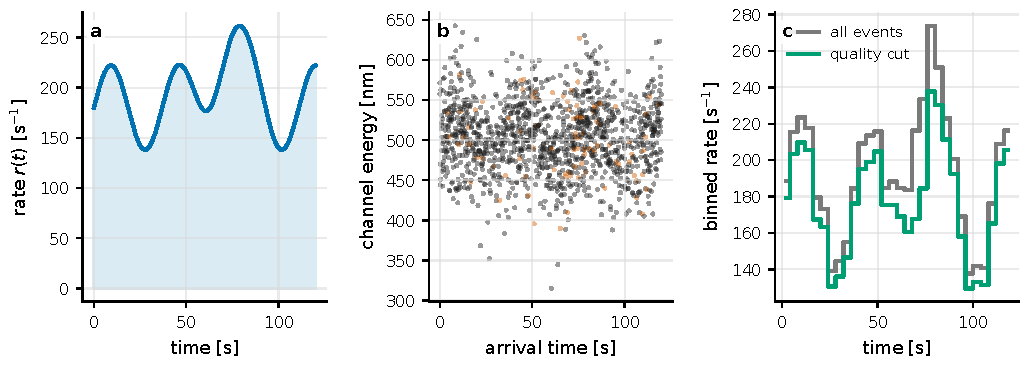
\includegraphics[width=0.96\linewidth]{figures/generated/chapter_20/ch20_event_table_simulation.pdf}
\caption{A simulated event table generated by an inhomogeneous Poisson process. The left panel is the input photon rate \(r(t)\); the middle panel retains each photon's arrival time, equivalent wavelength channel, and quality flag; the right panel projects the event table into a light curve and shows the effect of quality selection. The event table keeps channel and quality information beyond the light curve, so the same data can still be re-used for correlation, polarization, or energy-spectrum analysis.}
\label{fig:e26-eventtable}
\end{figure}

\section{The first computational experiment: build an event table, verify Poisson and shot noise}
\label{sec:e26-poisson}

The goal of the first experiment is the plainest yet the most important: \textbf{build by hand an event table that obeys Poisson statistics, then use it to verify Poisson statistics back}, thereby thoroughly digesting the shot noise of Chapter \ref{chap:e03}.

First, ``how to build.'' If the photon rate is constant at \(r\), the most economical way is to use a property of the Poisson process: the time interval between two adjacent photons follows an exponential distribution, \(P(\Delta t)=r\,e^{-r\Delta t}\). So from a uniform random number \(u\in(0,1)\) take \(\Delta t=-\ln(u)/r\), accumulate one after another, and obtain a string of arrival times. If the rate varies with time, \(r(t)\) (as in the left panel of Figure \ref{fig:e26-eventtable}), use \textbf{thinning}: first generate candidate photons at a constant rate \(r_{\max}\) higher than all times, then for each candidate independently ``keep or discard'' with probability \(r(t_i)/r_{\max}\). Those kept are one true realization of the inhomogeneous Poisson process. The virtue of this method is that it forces you to think through ``where the randomness comes from'' rather than tuning a black-box function.

Now verify. At constant rate, the number of photons \(N\) in a bin of length \(\Delta t\) follows the Poisson distribution, a known result of Chapter \ref{chap:e03}, used here by name:
\begin{equation}
  P(N)=\frac{\mu^{N}}{N!}\,e^{-\mu},\qquad \mu=r\,\Delta t .
  \label{eq:e26-poisson-pmf}
\end{equation}
\begin{formulaexplain}
\(P(N)\) is the probability of counting exactly \(N\) photons in a bin, and \(\mu\) is the \textbf{mean} photon number of this bin (equal to rate times bin width). The Poisson distribution is determined by the single parameter \(\mu\), which is both its mean and its variance, its most useful and most testable property.
\end{formulaexplain}
Grounding the symbols: \(N\) is a dimensionless count, \(\mu=\bar N\) is the dimensionless mean count, \(r\) has units \(\mathrm{s^{-1}}\), and \(\Delta t\) has units s. The place where the Poisson distribution can be verified at a glance is that its mean and variance are \textbf{equal}. We write this as a test quantity computable directly from data: the \textbf{Fano factor}:
\begin{equation}
  F=\frac{\operatorname{Var}(N)}{\langle N\rangle}\;\xrightarrow[\text{Poisson}]{}\;1 .
  \label{eq:e26-fano}
\end{equation}
\begin{formulaexplain}
\(\langle N\rangle\) is the sample mean of the bin counts, and \(\operatorname{Var}(N)\) is their sample variance. The Fano factor \(F\) is the ratio of the two. Pure Poisson (coherent light, shot-noise-dominated) gives \(F=1\); bunched thermal light gives \(F>1\), and antibunched nonclassical light gives \(F<1\).
\end{formulaexplain}
Why is the Poisson variance exactly equal to the mean? This is no coincidence and is worth deriving on the spot. From Eq.\ \eqref{eq:e26-poisson-pmf},
\[
  \langle N\rangle=\sum_{N=0}^{\infty}N\,\frac{\mu^N}{N!}e^{-\mu}
  =\mu\,e^{-\mu}\sum_{N=1}^{\infty}\frac{\mu^{N-1}}{(N-1)!}
  =\mu\,e^{-\mu}\,e^{\mu}=\mu,
\]
where we used the \textbf{exponential series expansion} \(\sum_{m\ge0}\mu^m/m!=e^{\mu}\) (substituting \(m=N-1\)). Similarly compute the second factorial moment:
\[
  \langle N(N-1)\rangle=\sum_{N=0}^{\infty}N(N-1)\frac{\mu^N}{N!}e^{-\mu}
  =\mu^2 e^{-\mu}\sum_{N=2}^{\infty}\frac{\mu^{N-2}}{(N-2)!}=\mu^2 .
\]
So \(\langle N^2\rangle=\langle N(N-1)\rangle+\langle N\rangle=\mu^2+\mu\), and substituting into the variance definition:
\[
  \operatorname{Var}(N)=\langle N^2\rangle-\langle N\rangle^2=(\mu^2+\mu)-\mu^2=\mu .
\]
The variance equals the mean, with not a step skipped. This is the origin of the famous shot-noise line ``\(\sigma_N=\sqrt{\bar N}\),'' and the basis of \(F\to1\) in Eq.\ \eqref{eq:e26-fano}.

Order of magnitude: if the event table you build has mean rate \(r=5\times10^{5}\,\mathrm{s^{-1}}\) and bin width \(\Delta t=1\,\mathrm{ms}\), then each bin has \(\mu=500\) photons, with relative fluctuation \(1/\sqrt{\mu}\simeq4.5\%\); shrink the bin width to \(1\,\mu\mathrm{s}\) and \(\mu=0.5\), most bins are empty, and the Fano test relies on the statistics of a large number of bins to be stable. \textbf{Common pitfall}: if you compute an \(F\) clearly deviating from 1, do not rush to declare that you have seen nonclassical light: more likely the detector \textbf{dead time} is at work. Dead time briefly ``blinds'' the detector after a photon, suppressing closely following counts and thereby artificially pushing the variance below the mean (\(F<1\)), disguising itself as antibunching. So this most basic experiment is in fact teaching you to distinguish ``physics'' from ``instrument.''

\section{Tabletop HBT: ``seeing'' bunching amid random coincidences}
\label{sec:e26-hbt}

The second experiment pushes Poisson to \textbf{second order}: with one beam of light, one beamsplitter, and two detectors, do a tabletop version of the Hanbury Brown--Twiss (HBT) experiment, measure \(g^{(2)}(\tau)\) by hand, and verify the bunching of Chapter \ref{chap:e08} \citep{1956Natur.178.1046H,1957RSPSA.242..300B,1963PhRv..130.2529G}.

First the picture. Each of the two intensity streams jitters randomly; why should there be a bit more ``common'' fluctuation near zero delay than elsewhere? Think of thermal light (or the \textbf{pseudothermal light} made by a rotating ground glass) as a superposition of many random-phase modes; its instantaneous intensity is not flat but jumps up and down. Within one \textbf{coherence time} \(\tau_c\), this one intensity fluctuation is \textbf{shared} by both detectors: in the instant of high intensity, both sides are more likely to each receive a photon, so ``coincidences'' increase near \(\tau=0\). Laser light is the exception: each of its modes is phase-locked, and the intensity is flat as a stagnant pool, so \(g^{(2)}(0)\simeq1\), no bunching \citep{1991PhRvL..67.1426N,1999PhRvA..60..674B,2024arXiv240418606N}.

How do we compute it from the event table? The method is to count \textbf{coincidence pairs} and normalize. Bin the two event tables by time difference \(\tau=t_j^{(2)}-t_i^{(1)}\) into a delay histogram \(H(\tau)\), then divide by an ``as-expected'' random baseline:
\begin{equation}
  \hat g^{(2)}(\tau)=\frac{H(\tau)}{H_{\rm bg}(\tau)},\qquad
  H_{\rm bg}\simeq R_1 R_2\,T\,\Delta\tau .
  \label{eq:e26-g2-estimator}
\end{equation}
\begin{formulaexplain}
\(H(\tau)\) is the number of photon pairs whose time difference falls in the \(\tau\)-th delay bin. \(H_{\rm bg}\) is the number of accidental coincidences there ``should'' be if the two streams were completely independent: the two rates \(R_1,R_2\) multiplied, times the total duration \(T\), times the delay-bin width \(\Delta\tau\). Dividing cancels the instrument's absolute counts, leaving only the excess \textbf{relative} to random coincidences.
\end{formulaexplain}
Grounding the symbols: \(R_1,R_2\) are the two single-count rates (\(\mathrm{s^{-1}}\)), \(T\) is the total integration time (s), \(\Delta\tau\) is the delay-bin width (s), and \(H,H_{\rm bg}\) are both dimensionless counts. The denominator \(H_{\rm bg}\) has a more reliable measured version: shift the second stream as a whole by an amount far greater than \(\tau_c\) and count coincidences again: by then the physical correlation has long vanished and what remains is purely accidental, which is the \textbf{time-shift background}. Normalizing by it automatically absorbs slow drifts.

The order of magnitude should give one confidence. Take \(R_1=R_2=5\times10^{5}\,\mathrm{s^{-1}}\), \(T=300\,\mathrm{s}\), \(\Delta\tau=0.5\,\mathrm{ns}\); then the accidental coincidences per delay bin are about
\[
  H_{\rm bg}\simeq (5\times10^5)^2\times300\times(0.5\times10^{-9})\approx3.75\times10^{4}\ \text{pairs/bin}.
\]
These pair counts themselves fluctuate as Poisson, with relative shot error about \(1/\sqrt{H_{\rm bg}}\simeq5\times10^{-3}\). So a peak of \(g^{(2)}-1\sim10^{-2}\) is visible above the noise on the tabletop, and this is exactly where the problem lies.

\begin{figure}[tbp]
\centering
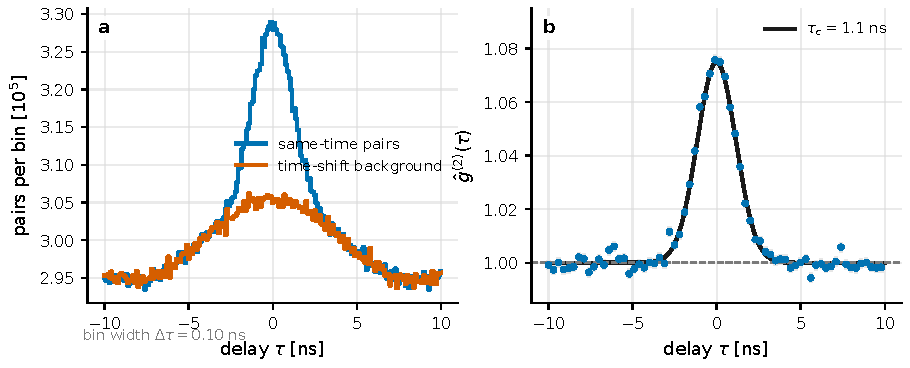
\includegraphics[width=0.96\linewidth]{figures/generated/chapter_20/ch20_hbt_lab_histogram.pdf}
\caption{The delay histogram of tabletop HBT. The left panel compares ``pairs/bin'' on the simultaneous time axis with the time-shift background; slow drifts appear in both curves and are therefore canceled by normalization. The right panel gives \(\hat g^{(2)}(\tau)\) after normalizing by the background histogram, with the peak width near zero delay set jointly by the source coherence time and the detector response.}
\label{fig:e26-hbt}
\end{figure}

\textbf{The deadliest pitfall: contrast dilution.} What a real instrument measures is not the ideal \(g^{(2)}\) but its shape after being \textbf{convolved} by the detector time response. If the coherence time \(\tau_c\) is far smaller than the electronics response width or the delay-bin width \(\Delta\tau\), the peak that thermal light should reach at 2 gets diluted, and the observed contrast shrinks approximately as \(\tau_c/\Delta\tau\). Here is the computation: a narrowband filter centered at \(416\,\mathrm{nm}\) with bandwidth \(\Delta\lambda=13\,\mathrm{nm}\) converts to \(\Delta\nu\simeq c\,\Delta\lambda/\lambda^2\approx2.3\times10^{13}\,\mathrm{Hz}\), so \(\tau_c\simeq1/\Delta\nu\approx4\times10^{-14}\,\mathrm{s}\); sampling with electronics of a few nanoseconds, the contrast is suppressed to \(\tau_c/\Delta\tau\sim10^{-5}\) in magnitude. This is why, if you see a tall, pretty peak on the tabletop, your first reaction should \textbf{not} be delight but the question: does it come from single-mode thermal light, or from electronics crosstalk, source slow drift, or a normalization chosen too conveniently? The intensity-interferometry analyses of VERITAS, MAGIC, and Asiago all, without exception, must explicitly handle this ledger of dilution, background, and dead time \citep{2009A&A...508..531N,2020NatAs...4.1164A,2024MNRAS.529.4387A,2017MNRAS.472.4126G}. This also incidentally explains the division of labor of the next section: the \(10^{-2}\) peak visible on the tabletop and the \(10^{-5}\) peak that must be dug out astronomically differ by five orders of magnitude.

\section{From tabletop to long baseline: simulating and fitting the uniform-disk visibility}
\label{sec:e26-disk}

Move HBT from the tabletop to between \textbf{two telescopes}, and it becomes an intensity interferometer (Chapter \ref{chap:e10}). The physics has not changed, still comparing whether two intensity streams fluctuate in sync, but now the two telescopes look at the same star of \textbf{finite angular size}. The longer the baseline, the more differently the two apertures see the coherent fluctuations, and the lower the zero-delay peak. This ``falling with baseline'' curve is precisely the visibility of the object's brightness distribution.

The Siegert relation of Chapter \ref{chap:e08} tells us that the excess of the second-order correlation equals the modulus squared of the first-order degree of coherence; the van Cittert--Zernike theorem of Chapter \ref{chap:e10} in turn tells us that the first-order spatial coherence \(\gamma_{12}\) between two telescopes is the Fourier transform of the object's normalized brightness distribution, that is, the visibility \(V\). Joining the two, the experimental procedure for estimating \(|V|^2\) from data is this: each baseline \(b\) first gives the zero-delay excess correlation \(\hat c_b=\hat g^{(2)}_b(0)-1\), then divides by the instrument contrast \(\hat\beta_b\) measured from that night's calibration star (or laboratory calibration):
\begin{equation}
  \widehat{|V_b|^2}=\frac{\hat c_b}{\hat\beta_b}.
  \label{eq:e26-v2-estimator}
\end{equation}
\begin{formulaexplain}
\(\hat c_b\) is the zero-delay excess correlation measured on baseline \(b\), and \(\hat\beta_b\) is the instrument contrast of the same baseline (folding in the dilution from time response, bandwidth, polarization selection, and efficiency). Dividing the two extracts the object's own \(|V_b|^2\). Note: \(\beta\) appears in the \textbf{denominator}, so its calibration error is \textbf{directly amplified} into the result.
\end{formulaexplain}
\(\hat c_b\), \(\hat\beta_b\), and \(|V_b|^2\) are all dimensionless. If a baseline's accidental-coincidence count is \(H_b\) and systematic error is momentarily ignored, then \(\sigma_{\hat c}\simeq H_b^{-1/2}\); but once the true contrast is as small as \(\beta\sim10^{-5}\), the same \(\sigma_{\hat c}\) is amplified into \(\sigma_{|V|^2}\simeq\sigma_{\hat c}/\beta\). \textbf{The pitfall of teaching simulations is precisely here}: to make the signal visible on the plot, you will be tempted to set \(\beta\) to a ``friendly'' value like \(0.05\), obtaining a \(g^{(2)}\) peak that pretends to be very clean; but the precision of the real astronomical \(|V|^2\) is still set by that true contrast of \(10^{-6}\)--\(10^{-5}\), the accidental-coincidence count, and the systematic floor. Writing this amplification factor in the most conspicuous place of the report when doing simulations is basic honesty.

Now build data and fit. The most commonly used source model is the \textbf{uniform disk}, whose visibility is the known result of Chapter \ref{chap:e11}, used by name:
\begin{equation}
  V(B_\perp)=\frac{2J_1(x)}{x},\qquad
  x=\frac{\pi\,\theta\,B_\perp}{\lambda},
  \label{eq:e26-uniform-disk}
\end{equation}
\begin{formulaexplain}
\(V\) is the visibility, \(J_1\) is the first-order Bessel function, and \(x\) is a dimensionless combination of angular diameter, baseline, and wavelength. The larger \(x\) (longer baseline or larger star), the smaller \(V\); \(2J_1(x)/x\) tends to 1 as \(x\to0\), and first vanishes at \(x=3.8317\). What one can obtain observationally is \(|V|^2\); the sign of the phase information is lost in intensity interferometry.
\end{formulaexplain}
Grounding each symbol: \(\theta\) is the angular diameter (rad, often written mas or \(\mu\mathrm{as}\) in reports), \(B_\perp\) is the projected baseline (m), \(\lambda\) is the observing wavelength (m), and \(J_1\) is dimensionless. Substituting the first zero \(x=3.8317\) gives the baseline most sensitive to angular diameter:
\[
  B_{\rm null}=\frac{3.8317}{\pi}\,\frac{\lambda}{\theta}\approx1.22\,\frac{\lambda}{\theta}.
\]
Plugging in real numbers: \(\lambda=416\,\mathrm{nm}\), \(\theta=1\,\mathrm{mas}=4.85\times10^{-9}\,\mathrm{rad}\),
\[
  B_{\rm null}\approx1.22\times\frac{416\times10^{-9}}{4.85\times10^{-9}}\ \mathrm{m}\approx105\,\mathrm{m}.
\]
This one number explains the whole landscape: the first zero of a \(1\,\mathrm{mas}\) bright star falls on a hundred-meter baseline, which is why hundred-meter-scale Cherenkov arrays like VERITAS can measure bright-star angular diameters; whereas the few-\(\mu\mathrm{as}\) angular radius of a Type Ia supernova pushes the first zero out to tens of kilometers, reachable only by kilometer-scale baselines. The \textbf{key point} when fitting is: \(|V|^2\) is most sensitive to \(\theta\) on the steep slope near the first zero, so if the baseline coverage all crowds into the \(V\approx1\) plateau region, the posterior will be very wide; spread the baselines to both sides of the zero and the angular diameter tightens up.

\begin{figure}[tbp]
\centering
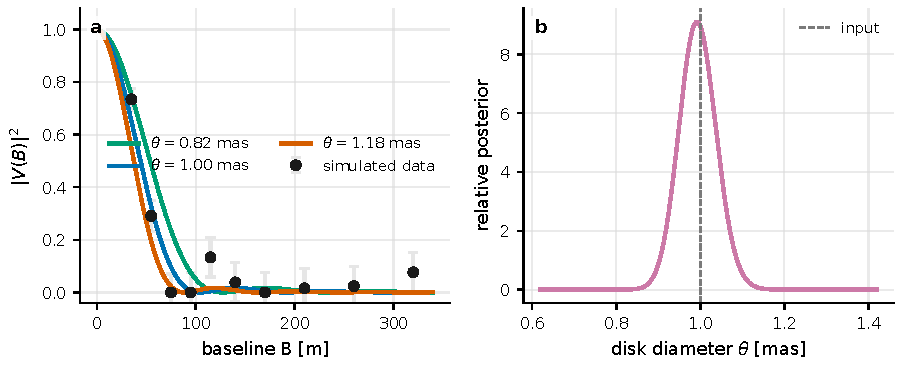
\includegraphics[width=0.96\linewidth]{figures/generated/chapter_20/ch20_uniform_disk_fit.pdf}
\caption{Intensity-interferometry fit of a uniform disk. The left panel simulates \(|V|^2\) measurements at various baselines for a target with \(\lambda=416\,\mathrm{nm}\), \(\theta=1\,\mathrm{mas}\); the slope is greatest and most sensitive to angular diameter near the first zero. The right panel converts these data into the angular-diameter posterior, whose width is set jointly by the \(|V|^2\) error, the baseline coverage, and the model assumptions.}
\label{fig:e26-disk}
\end{figure}

\section{Binaries and uv coverage: why multiple baselines and multiple epochs}
\label{sec:e26-binary}

The uniform disk has only one parameter; a binary makes the story interesting: it lets you see with your own eyes that although intensity interferometry loses the visibility's \textbf{sign} (phase), it still retains the \textbf{spatial frequency} that oscillates with baseline. The normalized squared visibility of two incoherent point sources is the known result of Chapters \ref{chap:e10}, \ref{chap:e11}:
\begin{equation}
  |V(\bm B_\perp)|^2=\frac{1+\rho^2+2\rho\cos\!\big(2\pi\,\bm B_\perp\!\cdot\!\bm s/\lambda\big)}{(1+\rho)^2},
  \label{eq:e26-binary}
\end{equation}
\begin{formulaexplain}
\(\rho=F_2/F_1\) is the flux ratio of the companion to the primary, \(\bm s\) is the angular-separation vector of the two stars, and \(\bm B_\perp\!\cdot\!\bm s/\lambda\) is the dimensionless phase projected onto the baseline direction. The cosine term in the numerator makes \(|V|^2\) oscillate along the baseline, and the denominator \((1+\rho)^2\) merely normalizes it to 1 at \(\bm B_\perp\to0\).
\end{formulaexplain}
Grounding the symbols and dimensions: \(\rho\) is dimensionless, \(\bm s\) is an angular vector (rad, often mas in reports), \(\bm B_\perp\) has units m, \(\lambda\) has units m, and the whole \(\bm B_\perp\!\cdot\!\bm s/\lambda\) is dimensionless. Look at two extremes to feel what it says. For an equal-brightness binary \(\rho=1\), Eq.\ \eqref{eq:e26-binary} reduces to \((1+\cos\phi)/2\), swinging from 1 all the way to 0 with phase: full modulation. If the companion has only a tenth of the primary's flux, \(\rho=0.1\), the cosine term makes \(|V|^2\) swing up and down about its mean, and this \textbf{oscillation half-amplitude} is
\[
  \frac{2\rho}{(1+\rho)^2}=\frac{2\times0.1}{1.1^2}\approx0.17,
\]
while the center of the swing (the mean) is \(\dfrac{1+\rho^2}{(1+\rho)^2}=\dfrac{1.01}{1.21}\approx0.835\). So \(|V|^2\) swings \(0.17\) on either side of the mean \(0.835\), actually rippling between about \(0.67\) and \(1\): the maximum \(1\) occurs at \(\cos\phi=1\), and the minimum \(\dfrac{(1-\rho)^2}{(1+\rho)^2}=\dfrac{0.81}{1.21}\approx0.67\) at \(\cos\phi=-1\), a peak-to-trough difference of about \(0.33\). The fainter the companion, the shallower the ripple, and the more it tests measurement precision. Compute the phase too: with \(B=180\,\mathrm{m}\), \(\lambda=500\,\mathrm{nm}\), separation \(0.5\,\mathrm{mas}=2.42\times10^{-9}\,\mathrm{rad}\),
\[
  \phi=2\pi\frac{B\,s}{\lambda}=2\pi\times\frac{180\times2.42\times10^{-9}}{500\times10^{-9}}\approx5.5\ \mathrm{rad},
\]
close to a full turn: a clear single oscillation period is visible on a single baseline.

But one baseline is only \textbf{one point} in the uv plane (Chapter \ref{chap:e11}). To simultaneously determine the magnitude and direction of the separation, the flux ratio, and the orbital geometry, one must spread out the uv coverage: multiple baselines sample different \(\bm B_\perp\) at a given instant, Earth rotation makes each baseline's projection \(\bm B_\perp(t)\) trace an arc over a night (\textbf{Earth-rotation aperture synthesis}), and multiple epochs let \(\bm s(t)\) sweep through different phases with orbital motion. This is the substance of the slogan ``multiple baselines, multiple epochs'': \textbf{use different uv samplings to pull apart the degenerate parameters one by one}. \textbf{Common pitfall}: if the uv coverage lies along only one direction, the separation in the perpendicular direction is essentially unconstrained, and the fit gives an elongated, misleading error ellipse: a nice-looking plot with untrustworthy parameters.

\begin{figure}[tbp]
\centering
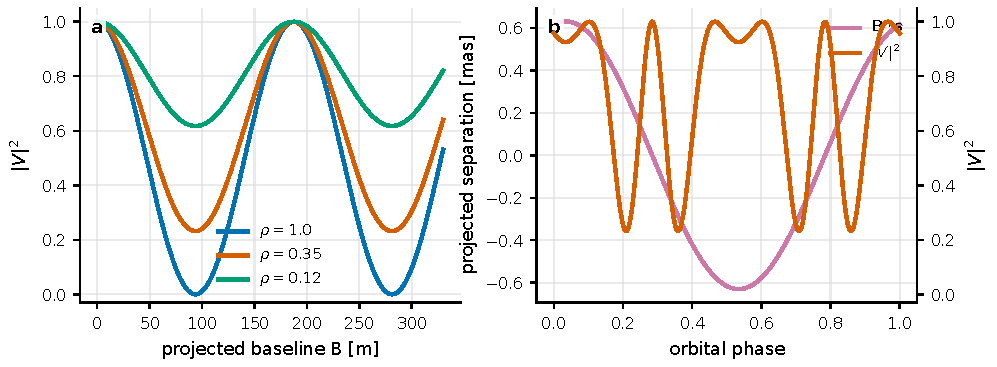
\includegraphics[width=0.96\linewidth]{figures/generated/chapter_20/ch20_binary_visibility.pdf}
\caption{The binary \(|V|^2\) case. The left panel shows how, at fixed angular separation, the flux ratio \(\rho\) controls the depth of the oscillation with baseline; the right panel shows how, in an inclined orbit, the projected separation \(\bm B\!\cdot\!\bm s\) varies with orbital phase, thereby changing \(|V|^2\) on a fixed baseline. Multi-baseline and multi-epoch data are used to separate the separation, the flux ratio, and the orbital geometry.}
\label{fig:e26-binary}
\end{figure}

\section{The correlator: turning the event table into a correlation function, and learning to doubt it}
\label{sec:e26-correlator}

The previous sections silently assumed ``we already have \(g^{(2)}(\tau)\).'' This section fills in the intermediate machine, the \textbf{correlator}, and stresses that half its value lies in \textbf{quality control}, not speed.

The correlator's task is a single sentence: turn two event tables into a batch of delay histograms, with every coincidence pair traceable back to the two original events and one time difference. There are three routes to implement it, all computing the same quantity but at different costs. The crudest double loop compares all event pairs, with computation growing as \(N_1 N_2\), absurdly slow. If events are already time-sorted, one compares only neighbors falling within the correlation window \(|t_j-t_i|<\tau_{\max}\), and the computation drops to about \(N_\gamma k\), where \(k\sim2R\tau_{\max}\) is the number of candidate pairs near each photon. The third route first projects events onto uniform time bins into a sequence, then does the cross-correlation via fast Fourier transform, with computation about \(M\log M\) (\(M=T/\Delta t\)). The three give consistent results, but their memory footprint, time resolution, and dead-time handling differ; this itself is a good comparison experiment.

Why is the engineering pressure so great? Two scalings explain everything. The \textbf{number of baselines} of a multi-telescope array grows quadratically with the number of telescopes (Chapter \ref{chap:e11}): 4 telescopes have only 6 baselines, but 60 have \(\binom{60}{2}=1770\). A single telescope's \textbf{raw data rate} swells as the time bin narrows and the spectral channels multiply:
\begin{equation}
  D\simeq \frac{N_\nu\,n_{\rm bit}}{\Delta t},
  \label{eq:e26-datarate}
\end{equation}
\begin{formulaexplain}
\(D\) is the single-stream data rate, \(N_\nu\) is the number of spectral channels retained simultaneously, \(n_{\rm bit}\) is the number of bits per time bin, and \(\Delta t\) is the time-bin width. The narrower the bin and the more the channels, the fiercer the data stream: this determines what hardware the correlation must lean on.
\end{formulaexplain}
Grounding the units: \(D\) has units \(\mathrm{bit\,s^{-1}}\), \(N_\nu\) is dimensionless, \(n_{\rm bit}\) is dimensionless, and \(\Delta t\) has units s. Plug in real numbers: with \(\Delta t=4\,\mathrm{ns}\), single channel \(N_\nu=1\), \(n_{\rm bit}=16\), \(D\simeq16/(4\times10^{-9})=4\times10^{9}\,\mathrm{bit\,s^{-1}}=4\,\mathrm{Gb\,s^{-1}}\); retaining 64 spectral channels at once, a single telescope surges to \(256\,\mathrm{Gb\,s^{-1}}\). This is why modern intensity interferometry is inseparable from GPU/FPGA real-time correlation, tiered triggering, on-chip accumulation, or strict compression: MAGIC's real-time dead-time-free correlator and VERITAS's online/offline pipelines were both forced into being by this data rate \citep{2020NatAs...4.1164A,2024MNRAS.529.4387A,2024ApJ...966...28A}.

\begin{figure}[tbp]
\centering
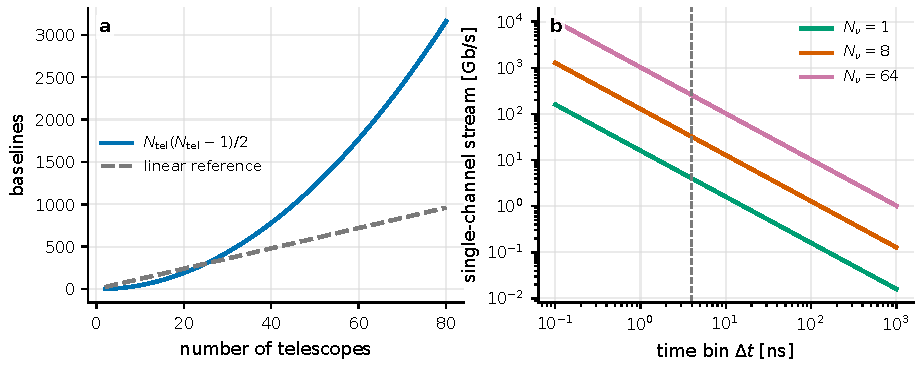
\includegraphics[width=0.96\linewidth]{figures/generated/chapter_20/ch20_correlator_scaling.pdf}
\caption{The two scalings of a multi-telescope correlator. Left: the number of baselines grows quadratically with the number of telescopes, so expanding the array rapidly increases the correlation load. Right: the single-stream data flow rises as the time bin narrows and the spectral channels multiply; nanosecond sampling plus tens of spectral channels has already entered the regime that must be handled by real-time hardware or GPUs.}
\label{fig:e26-correlator}
\end{figure}

What truly sets this section apart from the earlier ones is the \textbf{null test}, and it should be graded as seriously as the result plots, not a token in the appendix. At minimum one should do these: shift the second stream as a whole by a time far greater than \(\tau_c\), and the real peak \textbf{must vanish}; cap the light or run the same pipeline with no starlight, and electronics crosstalk \textbf{should not} produce a zero-delay peak; scramble the polarization or spectral channels, and only the physically correlated channel should retain signal; slice the data by time, and \(\hat g^{(2)}(0)-1\) should converge smoothly as \(T^{-1/2}\) with integration time, rather than concentrating in one short segment. These tests directly determine whether a peak can be interpreted as an astronomical signal: the tabletop/in-sky experiments of Guerin et al., the photon-counting schemes of AQuEye/IquEye, and the intensity interferometry of modern Cherenkov arrays all treat them as part of the result \citep{2017MNRAS.472.4126G,2016SPIE.9907E..0NZ,2021MNRAS.506.1585Z,2020NatAs...4.1164A}. \textbf{One line of discipline}: a small peak that passes the null test is worth far more than a big peak that does not.

\section{Numerically demonstrating SPADE: the information is not in the brightest pixel}
\label{sec:e26-spade}

Now switch to a seemingly unrelated but actually cognate experiment, echoing Chapter \ref{chap:e12}. Earlier we used long baselines to reach high spatial frequencies; here the question is reversed: \textbf{we have already imaged, and two point sources sit closer than the point-spread function; can we still measure their separation?} The answer from direct imaging is disheartening, but mode sorting (SPADE) will tell you the information was there all along: just not in those few bright pixels you were staring at.

First the picture. Two equal-brightness, incoherent point sources with separation \(s\) far smaller than the point-spread-function (PSF) width \(\sigma\) produce a combined image in the focal plane that is almost just ``a little bit fatter.'' The trouble is that the \textbf{derivative} of the pixel intensity with respect to \(s\) tends to zero as \(s\to0\): the parameter you want to estimate barely changes what you measure, so the Fisher information collapses toward zero. This is the statistically precise meaning of the \textbf{Rayleigh curse}: not ``cannot be resolved,'' but ``the measurement mode of direct imaging wastes the information about \(s\)'' \citep{2015Optic...2..646T,2016PhRvX...6c1033T}.

SPADE uses a different measurement: not measuring pixel intensity but projecting the light onto a set of \textbf{Hermite--Gaussian modes} and counting the photons in each mode. For a Gaussian PSF and equal-brightness two-point sources, this is the known result of Chapter \ref{chap:e12}: the probability of landing in the \(n\)-th mode is Poisson-shaped:
\begin{equation}
  p_n=e^{-\Gamma}\,\frac{\Gamma^{\,n}}{n!},\qquad
  \Gamma=\left(\frac{s}{4\sigma}\right)^{\!2}.
  \label{eq:e26-spade-prob}
\end{equation}
\begin{formulaexplain}
\(p_n\) is the probability that a photon is projected onto the \(n\)-th Hermite--Gaussian mode, with \(n=0,1,2,\dots\) the transverse mode index. \(\Gamma\) is a dimensionless small quantity blending the separation with the PSF width. The smaller the separation, the smaller \(\Gamma\), and the vast majority of photons still land in the fundamental mode \(n=0\); but the little bit of probability of \(n\ge1\) is extremely sensitive to \(s\).
\end{formulaexplain}
Grounding the symbols: \(s\) is the angular separation (in the same angular units as \(\sigma\), or the same focal-plane length units), \(\sigma\) is the Gaussian PSF width, and \(\Gamma\), \(p_n\) are dimensionless. Plug in numbers: at \(s=0.2\sigma\), \(\Gamma=(0.2/4)^2=2.5\times10^{-3}\), so \(p_1\approx\Gamma=2.5\times10^{-3}\), and only two or three out of a thousand photons make it into the \(n=1\) mode, but it is precisely these two or three photons that carry almost all the information about \(s\).

Why does the information not collapse? Compute the Fisher information of the Poisson probability \eqref{eq:e26-spade-prob} step by step. The Fisher information of a single photon about the parameter \(s\) is
\[
  I_{\rm SPADE}(s)=\sum_{n}\frac{1}{p_n}\!\left(\frac{\partial p_n}{\partial s}\right)^{\!2}.
\]
Using a standard fact about the Poisson distribution, the Fisher information of the Poisson mean \(\Gamma\) itself is \(1/\Gamma\), together with the chain rule \(I_s=(d\Gamma/ds)^2\cdot(1/\Gamma)\). Substituting \(\Gamma=s^2/(16\sigma^2)\), so \(d\Gamma/ds=s/(8\sigma^2)\), we get
\[
  I_{\rm SPADE}(s)=\frac{\big(s/8\sigma^2\big)^2}{s^2/(16\sigma^2)}
  =\frac{s^2/(64\sigma^4)}{s^2/(16\sigma^2)}=\frac{16\sigma^2}{64\sigma^4}=\frac{1}{4\sigma^2}.
\]
Not a step skipped, and the result is astonishingly clean: \(I_{\rm SPADE}=1/(4\sigma^2)\), \textbf{independent of the separation \(s\)}: even as \(s\to0\), the information carried by each photon does not decay. By contrast, the Fisher information of direct imaging collapses toward zero as \(s\to0\). This is the whole secret of how SPADE crosses the Rayleigh curse.

\begin{figure}[tbp]
\centering
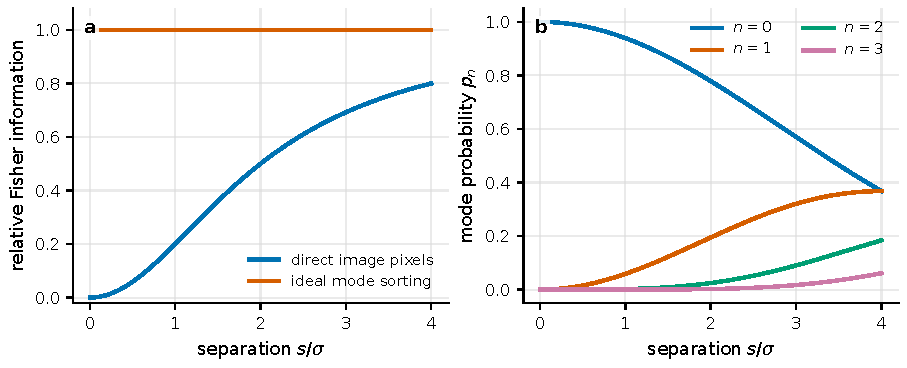
\includegraphics[width=0.96\linewidth]{figures/generated/chapter_20/ch20_spade_computational_experiment.pdf}
\caption{The SPADE computational experiment. The left panel compares the relative Fisher information of direct pixel imaging and ideal mode sorting at small separation: direct imaging loses information as \(s/\sigma\ll1\), while mode sorting stays near constant. The right panel shows the Hermite--Gaussian mode probabilities; at very small separation the higher-mode probabilities are small but have nonzero slope, so a highly stable, low-crosstalk mode measurement is required.}
\label{fig:e26-spade}
\end{figure}

\textbf{A pitfall you must write into the code}: the pretty constant curve above is the \textbf{ideal} case. In a real system, the mode basis does not perfectly match the true PSF, the centering has errors, there are aberrations, and there is background light: any \textbf{mode crosstalk} lets a bit of the light that should be in the clean \(n=1\) mode leak into \(n=0\), thereby laying down an \textbf{information floor} for the Fisher information and flattening the \(s\to0\) advantage. So teaching code should not plot only the ideal curve but add a tunable crosstalk parameter, letting students watch the information floor rise as the crosstalk increases. For precisely this reason, SPADE is currently better suited as a computational experiment and pathfinder than as a promise that the next-generation telescope can losslessly reach the quantum limit \citep{2016OExpr..24.3684N,2017PhRvL.118g0801T}.

\section{Capstone project: how the Type Ia distance toy model strings together the whole error budget}
\label{sec:e26-typeia}

The final project assembles the previous parts into a whole machine, and deliberately exposes the danger a toy model most easily conceals: angular radius, velocity, and explosion time look as if they differ only by a proportionality constant, but the real errors come from \textbf{different instruments, different models, different epochs}. This is the idea of using the expanding-photosphere method to measure the angular-diameter distance of a Type Ia supernova \citep{2025PhRvD.111h3047K}.

The physical chain is this: the spectral model gives the photospheric expansion velocity \(v_{\rm ph}(t)\), intensity interferometry gives the photospheric angular radius \(\theta_{\rm ph}(t)\), and comparing the two yields the angular-diameter distance:
\begin{equation}
  \theta_{\rm ph}(t)=\frac{R_{\rm ph}(t)}{D_A}\simeq\frac{v_{\rm ph}\,(t-t_0)}{D_A}.
  \label{eq:e26-typeia-theta}
\end{equation}
\begin{formulaexplain}
\(\theta_{\rm ph}\) is the photospheric angular radius, \(R_{\rm ph}\) is the physical radius, \(D_A\) is the angular-diameter distance, and \(t_0\) is the explosion time. If the photosphere expands at approximately constant velocity \(v_{\rm ph}\), the physical radius is about velocity times time; dividing it by the angular radius extracts the distance.
\end{formulaexplain}
Grounding the symbols and dimensions: \(v_{\rm ph}\) has units \(\mathrm{cm\,s^{-1}}\), about \(8\times10^8\)--\(1.5\times10^9\,\mathrm{cm\,s^{-1}}\) for a normal Type Ia at early times; \(t-t_0\) has units s or d, and intensity interferometry is most interested in a few days to a few tens of days after explosion; \(D_A\) is in Mpc; and \(\theta_{\rm ph}\) is usually a few to a few tens of \(\mu\mathrm{as}\). Plug in real numbers: \(v_{\rm ph}=10^{9}\,\mathrm{cm\,s^{-1}}\), \(t-t_0=15\,\mathrm{d}=1.30\times10^{6}\,\mathrm{s}\), the physical radius \(R_{\rm ph}\approx1.30\times10^{15}\,\mathrm{cm}\); then take \(D_A=20\,\mathrm{Mpc}=6.17\times10^{25}\,\mathrm{cm}\),
\[
  \theta_{\rm ph}\approx\frac{1.30\times10^{15}}{6.17\times10^{25}}\ \mathrm{rad}
  \approx2.1\times10^{-11}\,\mathrm{rad}\approx4.3\,\mu\mathrm{as}.
\]
At \(\lambda=500\,\mathrm{nm}\), this corresponds to a first-zero baseline scale \(\lambda/\theta\sim24\,\mathrm{km}\). If one is willing to use the whole visibility curve rather than only wait for the first zero, kilometer-to-ten-kilometer baselines still have science to mine, but the error budget is stretched extremely tight.

How do we combine the angular radius and velocity into a distance posterior? Write a joint likelihood that simultaneously penalizes the inconsistency of the ``angular-radius prediction'' and the ``velocity prediction'':
\begin{equation}
  \ln{\cal L}(D_A)=
  -\frac12\sum_k\!\left[\frac{\hat\theta_k-v_{{\rm ph},k}(t_k-t_0)/D_A}{\sigma_{\theta,k}}\right]^2
  -\frac12\sum_k\!\left[\frac{\hat v_k-v_{{\rm ph},k}}{\sigma_{v,k}}\right]^2 .
  \label{eq:e26-typeia-like}
\end{equation}
\begin{formulaexplain}
\(D_A\) is the distance to be estimated, \(\hat\theta_k\) and \(\hat v_k\) are the angular radius and velocity measured at the \(k\)-th epoch, and \(\sigma_{\theta,k}\), \(\sigma_{v,k}\) are their respective errors. The first sum enforces ``the angular radius must match \(v(t-t_0)/D_A\),'' and the second enforces ``the velocity model must match the measured velocity.'' Minimizing both together is what constrains \(D_A\).
\end{formulaexplain}
Grounding the symbols: \(\hat\theta_k\) comes from the \(|V|^2\) fit of the \(k\)-th epoch (the machinery of Eqs.\ \eqref{eq:e26-v2-estimator}, \eqref{eq:e26-uniform-disk}), with units rad or \(\mu\mathrm{as}\); \(\hat v_k\) comes from spectral-line velocity or a radiative-transfer model, with units \(\mathrm{cm\,s^{-1}}\); and \(\sigma_{\theta,k}\), \(\sigma_{v,k}\) each \textbf{simultaneously} contain statistical error and model systematic error. \textbf{The biggest pitfall of the toy model} is right here: if you lazily add only a \(10\%\) Gaussian noise to \(\hat\theta\), you will get a posterior so narrow it is distorted. A real project must have students turn those ``invisible knobs'': vary the explosion time \(t_0\), add a velocity gradient, put in non-spherical asymmetry, replace the uniform disk with a limb-darkened brightness distribution, and then watch the posterior widen bit by bit. The posterior \textbf{should} widen; that is what an honest error budget looks like.

\begin{figure}[tbp]
\centering
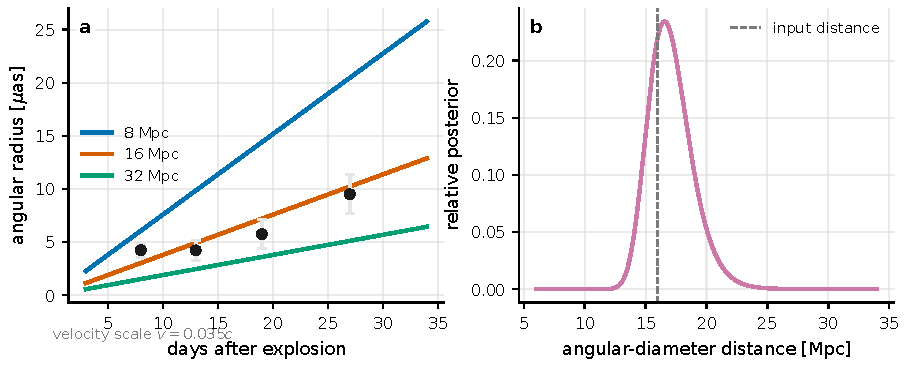
\includegraphics[width=0.96\linewidth]{figures/generated/chapter_20/ch20_typeia_distance_posterior.pdf}
\caption{The Type Ia supernova angular-diameter-distance toy model. The left panel uses a simplified expansion model with \(v_{\rm ph}=0.035c\), giving the angular radius versus time at various distances, with simulated angular-radius measurements overlaid; the right panel combines these angular radii with the velocity model into a \(D_A\) posterior. A real analysis must replace the constant-velocity shell with a radiative-transfer model, and write non-spherical asymmetry, the line-forming layer, and the baseline coverage into the error budget.}
\label{fig:e26-typeia}
\end{figure}

These five projects strung together are exactly a course line of increasing difficulty: first use an LED, pseudothermal light, and a laser to measure \(g^{(2)}(\tau)\), verifying Poisson and bunching; then practice time-shift background, quality selection, and \(T^{-1/2}\) convergence on the same event table; enter spatial coherence and fit the \(|V|^2\) of a uniform disk and a binary, feeling the role of baseline coverage; then do SPADE, seeing how the Fisher information escapes the Rayleigh curse and how it is pressed back to the floor by crosstalk; and finally use the Type Ia toy model to propagate together the uncertainties of angular radius, velocity, and explosion time. Each project's deliverables are equally plain: one event-table description, one runnable script, a set of plots, one short report citing real literature, and \textbf{at least two null tests}. Remember the line that recurs throughout this chapter: code that runs is only the first hurdle; a plot that cannot account for its time reference, \(\beta\) calibration, crosstalk matrix, or systematic error can be generated, but cannot be treated as an astronomical measurement.

\section*{Chapter Summary}
\addcontentsline{toc}{section}{Chapter Summary}

\begin{itemize}
  \item \textbf{Everything begins with the event table.} Each photon leaves a time, a channel, a polarization, and a quality flag; the light curve is only one lossy projection of it (Eq.\ \eqref{eq:e26-binned-count}). Bin first, and you can never go back.
  \item \textbf{Poisson's signature is variance equals mean.} Use the Fano factor \(F=\operatorname{Var}/\langle N\rangle\to1\) to test shot noise (Eq.\ \eqref{eq:e26-fano}); \(F<1\) is often dead-time disguised as antibunching, not new physics.
  \item \textbf{Bunching is seen via coincidence excess, but gets diluted.} \(\hat g^{(2)}\) is normalized by the time-shift background (Eq.\ \eqref{eq:e26-g2-estimator}); when the coherence time is far smaller than the response width, the thermal-light peak shrinks by \(\tau_c/\Delta\tau\) to the \(10^{-5}\) level.
  \item \textbf{Visibility is the object's Fourier fingerprint.} \(|V|^2\) is obtained from \(\hat g^{(2)}(0)-1\) divided by the instrument contrast \(\beta\) (Eq.\ \eqref{eq:e26-v2-estimator}); \(\beta\) is in the denominator, so its calibration error is directly amplified. The uniform-disk first zero \(B_{\rm null}\approx1.22\lambda/\theta\) (Eq.\ \eqref{eq:e26-uniform-disk}), and a \(1\,\mathrm{mas}\) bright star is at about a hundred-meter baseline.
  \item \textbf{Multiple baselines, multiple epochs are for breaking degeneracies.} The binary's oscillation half-amplitude \(2\rho/(1+\rho)^2\) (Eq.\ \eqref{eq:e26-binary}) shallows as the companion dims; single-direction uv coverage gives an elongated, misleading error ellipse.
  \item \textbf{Half the correlator's value is the null test.} Time shift, capping, channel scrambling, and \(T^{-1/2}\) convergence must all be graded like the results; the data-rate scaling (Eq.\ \eqref{eq:e26-datarate}) explains why real-time hardware is a must.
  \item \textbf{SPADE frees information from the bright pixels.} The mode probabilities are Poisson-shaped (Eq.\ \eqref{eq:e26-spade-prob}), and the Fisher information \(1/(4\sigma^2)\) is independent of separation; but crosstalk lays down an information floor, so the ideal curve cannot be trusted lightly.
  \item \textbf{The capstone tests the error budget, not the fit.} In the Type Ia distance toy model (Eqs.\ \eqref{eq:e26-typeia-theta}, \eqref{eq:e26-typeia-like}), the posterior \textbf{should} widen once you put in real systematic errors; if it does not, you have not yet put the danger in.
\end{itemize}

\medskip
\noindent\textbf{Questions to Ponder:} (1) You measure \(F=0.7\); give at least two physically distinct explanations, and design an experiment to distinguish each pair. (2) If a binary's companion flux ratio drops from \(\rho=0.3\) to \(\rho=0.05\), by roughly what factor must the accidental-coincidence count \(H\) increase to maintain the same oscillation significance? (3) Adding \(1\%\) mode crosstalk in SPADE, to what order of magnitude does the information floor push up the smallest resolvable \(s/\sigma\)?

\chapter{Common Misconceptions}
\label{chap:e27}

\begin{chapteropening}
By this point in the book, the toolbox is full: Poisson statistics, coherent and thermal states, \(g^{(1)}\) and \(g^{(2)}\), the Siegert relation, intensity interferometry, SPADE, Fisher information, event tables, and correlators. But the handier the tools, the easier it is to stumble in the last mile: mistaking ``counting photons'' for ``doing quantum astronomy,'' mistaking \(g^{(2)}\simeq1\) for ``this is a laser,'' mistaking one accidental high count for ``new physics.'' These pitfalls share a common feature: they all lie \emph{right next door to the correct conclusion}, one step away from falling in. This chapter introduces no new physical content in any formula; instead it takes the conclusions already rigorously established in the previous chapters and places each, one by one, beside the scene ``most easily misread,'' making clear \textbf{where each misconception goes wrong and what the correct physical picture is}. After reading this chapter, your tools will not grow in number, but your probability of using them wrongly will drop markedly.
\end{chapteropening}


\section{Why ``counting photons'' does not equal ``doing quantum astronomy''}
\label{sec:e27-photon-not-quantum}

First, a most common and most insidious misunderstanding: that merely because a detector can ``count out'' photons one by one, one is already standing inside the door of quantum astronomy.

The single-photon detector is indeed the entrance, but it is only the entrance. As Chapter \ref{chap:e13} explained, the raw product an instrument that counts photons hands us is an \textbf{event table} (event list): each row records one detected photon, carrying its arrival time \(t\) (units s or ns), detector/telescope index \(d\), frequency channel \(\nu\) (units Hz or channel number), and polarization label \(p\). Quantum information \emph{may} be hidden in this table, but whether it is hidden there, and whether it is extracted, depends on how you process the table afterward.

Consider two ways of processing. First: bin the event table in time, count how many rows are in each bin, and obtain a count-rate curve
\[
  R=\frac{N_\gamma}{T},
\]
where \(N_\gamma\) is the total photon count, \(T\) is the observing duration (s), and \(R\) has units \({\rm s}^{-1}\). This is an ordinary light curve, no different in essence from the magnitude curve measured on photographic plates a century ago: you have merely used a more expensive instrument to re-count ``how bright it is on average.'' Second: instead of counting the total, ask about the relation \emph{between} events: whether photons in two detectors and two time gates fire together more than coincidence would allow. This is what the \(g^{(2)}\) of Chapter \ref{chap:e08}, the intensity interferometry of Chapter \ref{chap:e10}, and the mode measurement of Chapter \ref{chap:e12} do. The criterion is blunt: \textbf{look at whether those labels truly enter the model}. If \(t,d,\nu,p\) are all summed away in the analysis, leaving only an average rate, then no matter how advanced the detector, what you are doing is still classical photometry.

Here let us dismantle a twin misunderstanding along the way: equating ``very few photons'' directly with ``quantum.'' X-ray and gamma-ray astronomy have for decades worked at low photon numbers, doing spectral fits with Poisson counting and the Cash likelihood \citep{1979ApJ...228..939C,1986ApJ...303..336G}, but the target of most such analyses is still average intensity or energy spectrum, classical quantities, only with a Poisson noise model. Conversely, radio and millimeter-wave astronomy often work in the \emph{high}-occupation, near-classical wave limit, yet can seriously discuss coherence functions, phase, polarization, and quantum noise. So ``few photons'' and ``quantum'' are two different yardsticks: the key distinction lies not in photon number but in \textbf{whether the model requires the joint probability of multiple photons or the modes of the light field to express it}.

There is a third, related pitfall: believing that ``once you have an event table, new physics will spontaneously appear.'' It will not. The Poisson model of Chapter \ref{chap:e03} stands ready: the expected count of the \(k\)-th bin in an observation is
\[
  \mu_k=R_k\,E_k\,\Delta t_k,
\]
where \(R_k\) is the instantaneous rate of that bin (\({\rm s}^{-1}\)), \(\Delta t_k\) is the bin width (s), \(E_k\) is the dimensionless effective-exposure factor (absorbing clouds, dead time, and the selection function), and \(\mu_k\) itself is dimensionless. A common erroneous operation is: compare all \(N_k\) against \emph{one and the same} constant \(\mu\), find the variance too large, and declare ``non-Poisson, new physics.'' But as long as the source is intrinsically variable (\(R_k\) varying with time), or the weather and dead time make \(E_k\) vary, then \(\mu_k\) \emph{should} differ bin by bin: the ``constant \(\mu\)'' you compared against was the wrong baseline from the start. What one should really do is let the model absorb these ordinary variations, then look at the residuals. Bayesian Blocks, period searches, and likelihood-ratio tests can all handle such problems, but each has its own conditions of applicability and its own number of trials \citep{2013ApJ...764..167S,1982ApJ...263..835S,1992ApJ...398..146G,2002ApJ...571..545P}, a point we return to reckon with in the last section of this chapter.

One line to close this section: \textbf{being able to count photons only means you have obtained the raw material; the new information of quantum astronomy is hidden in the joint distribution among events; if the labels do not enter the model, no matter how accurately the photons are counted, it is in vain.}


\section{\texorpdfstring{Why \(g^{(2)}\simeq1\) proves nothing}{Why g2 approximately equal to 1 proves nothing}}
\label{sec:e27-g2}

The second pitfall is almost a ``must-fall'' item for beginners in quantum optics: seeing \(g^{(2)}(0)\simeq1\), one either blurts out ``this is a coherent laser'' or conversely asserts ``there is no quantum nature at all.'' Both statements are untenable.

First lay out the rigorous conclusion of Chapter \ref{chap:e08}. A coherent state (the model of an ideal single-mode laser) does give a Poisson photon-number distribution and \(g^{(2)}(0)=1\). But this statement cannot be read in reverse: \(\mathbf{g^{(2)}(0)=1}\) \textbf{is not the unique fingerprint of a coherent state}. Thermal light (the chaotic light source of a star), when single-mode, has \(g^{(2)}(0)=2\); but once many modes are superposed, or the detector averages away the coherence fluctuations far shorter than its own response time, that ``bunching peak'' exceeding 1 is rapidly diluted, and the measured \(g^{(2)}(0)\) approaches 1 arbitrarily closely. That is, \(g^{(2)}\simeq1\) could be genuinely coherent light, or it could be thermal light diluted beyond recognition: from this number alone, you cannot tell which.

Write the dilution as a formula and the physical picture becomes clear. Chapter \ref{chap:e08} gave the basic form of contrast dilution; here we use its practical version:

\begin{equation}
  g^{(2)}_{\rm meas}(0)-1
  \;\simeq\;
  \frac{g^{(2)}_{\rm src}(0)-1}{M_{\rm eff}},
  \qquad
  M_{\rm eff}\simeq M_\perp\,M_\nu\,M_{\rm pol}\,\frac{\Delta t_{\rm eff}}{\tau_c}.
  \label{eq:e27-dilution}
\end{equation}
\begin{formulaexplain}
\(g^{(2)}_{\rm src}\) is the source's own second-order coherence (2 for single-mode thermal light), \(g^{(2)}_{\rm meas}\) is what the detector actually measures; \(M_{\rm eff}\) is the effective number of modes averaged over within the correlation bin, and \(M_\perp,M_\nu,M_{\rm pol}\) are respectively the numbers of spatial, frequency, and polarization modes, while \(\Delta t_{\rm eff}/\tau_c\) is the number of temporal modes smeared over. The more modes, the lower the bunching peak is pressed.
\end{formulaexplain}

Ground each symbol and plug in real numbers. The numerator on the right, \(g^{(2)}_{\rm src}(0)-1\), equals 1 for single-mode thermal light (dimensionless), the ``full-scale contrast when undiluted.'' The denominator \(M_{\rm eff}\) is the dimensionless effective number of modes, folding in all four averagings at once: spatially, if the telescope simultaneously collects several coherence patches of the source, \(M_\perp>1\); in frequency, if the filter admits several coherence bandwidths, \(M_\nu>1\); in polarization, if no selection is made, \(M_{\rm pol}\approx2\); and in time, if the detector response or correlation-bin width \(\Delta t_{\rm eff}\) (s) is far greater than the coherence time \(\tau_c\) (s), it averages \(\Delta t_{\rm eff}/\tau_c\) mutually incoherent wave trains into one.

Now plug in numbers. Chapter \ref{chap:e08} computed with \(\tau_c\simeq1/\Delta\nu=\lambda^2/(c\,\Delta\lambda)\): a \(1\,{\rm nm}\) narrowband filter near \(500\,{\rm nm}\) gives \(\tau_c\sim0.8\,{\rm ps}\) (\(\Delta\nu\sim1.2\times10^{12}\,{\rm Hz}\)); if the filter is widened to \(10\,{\rm nm}\), the bandwidth increases tenfold and \(\tau_c\) shrinks to a tenth, about \(8\times10^{-14}\,{\rm s}\), that is, of order \(10^{-13}\,{\rm s}\). Fast-electronics correlation bins are usually \(\Delta t_{\rm eff}\sim10^{-9}\)--\(10^{-8}\,{\rm s}\). So the time factor alone contributes
\[
  \frac{\Delta t_{\rm eff}}{\tau_c}\sim\frac{10^{-9}}{10^{-13}}
  =10^{4}
  \quad\text{to}\quad
  \frac{10^{-8}}{10^{-13}}=10^{5}.
\]
Even if space, frequency, and polarization are all made ``single-mode'' (\(M_\perp=M_\nu=M_{\rm pol}=1\)), the measured contrast is only
\[
  g^{(2)}_{\rm meas}(0)-1\sim\frac{1}{10^{4}\text{--}10^{5}}
  \sim10^{-4}\text{--}10^{-5},
\]
and stacking on the multimode factors, falling to \(10^{-5}\)--\(10^{-6}\) is the norm. So the \(g^{(2)}(0)\) of stellar thermal light \emph{should} sit right against 1, and the tiny excess is a signal to be found in the fifth or sixth decimal place. The Guerin group's starlight-bunching experiments, the AQuEye/IquEye schemes, and the intensity interferometry of VERITAS and MAGIC all treat this dilution as a \emph{core quantity}, not as evidence of ``no quantum nature'' \citep{2017MNRAS.472.4126G,2016SPIE.9907E..0NZ,2020NatAs...4.1164A,2021MNRAS.506.1585Z,2024MNRAS.529.4387A,2024ApJ...966...28A}. Figure \ref{fig:e27-g2-scaling} draws out this dilution chain.

\begin{figure}[tbp]
\centering
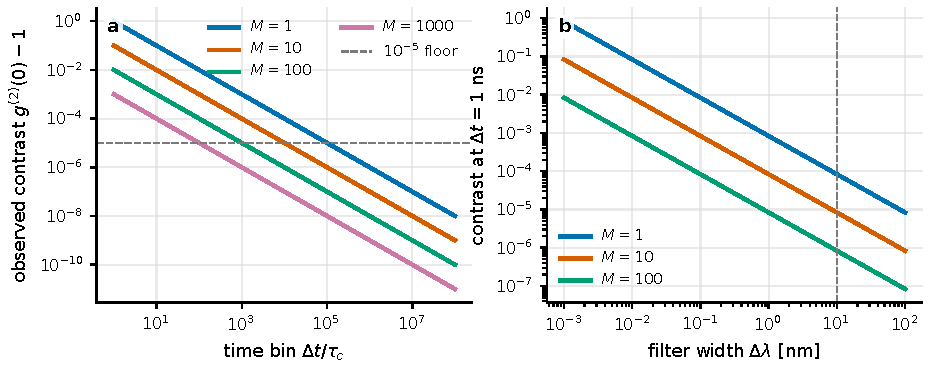
\includegraphics[width=0.96\linewidth]{figures/generated/chapter_21/ch21_g2_scaling_mistake.pdf}
\caption{How the time bin, spectral bandwidth, and mode number dilute the contrast of \(g^{(2)}\). The left panel shows how \(\Delta t/\tau_c\) and \(M_{\rm eff}\) press the bunching peak of single-mode thermal light down; the dashed line marks the \(10^{-5}\)-level systematic-error floor. The right panel converts the filter bandwidth into coherence time: at \(1\,{\rm ns}\) sampling, the thermal peak of broadband visible light easily falls below the calibratable range. This is precisely the true origin of ``\(g^{(2)}\simeq1\)'': not the absence of quantum nature, but the quantum nature being averaged and diluted away.}
\label{fig:e27-g2-scaling}
\end{figure}

Then what is a \textbf{truly ironclad nonclassical criterion}? The answer is antibunching, that is,
\[
  g^{(2)}(0)<1.
\]
Chapter \ref{chap:e08} proved: any classical random intensity satisfies \(g^{(2)}(0)\ge1\) (a direct consequence of the Cauchy--Schwarz inequality), so \(g^{(2)}(0)<1\) is something classical light \emph{can never do}: it means photons ``avoid'' one another, the signature of a single quantum emitter. The resonance-fluorescence experiment of Kimble, Dagenais, and Mandel first firmly established antibunching precisely by measuring \(g^{(2)}(0)<1\) \citep{1977PhRvL..39..691K}. But seeing antibunching in astronomical light sources is nearly impossible: the light of an object is usually the result of a vast number of independent emitters, countless propagation paths, and finite detector response all mixed together, and any sub-Poisson feature of a single quantum emitter is diluted beyond visibility by that enormous \(M_{\rm eff}\) in Eq.\ \eqref{eq:e27-dilution}.

So the lesson of this section is bidirectional: an astronomical report that writes ``\(g^{(2)}\simeq1\), therefore this is a laser,'' or writes ``\(g^{(2)}\simeq1\), therefore there is no quantum information,'' has no basis for either statement. \(\mathbf{g^{(2)}\simeq1}\) \textbf{is the default result after dilution; it neither proves coherence nor disproves quantumness; only }\(\mathbf{g^{(2)}(0)<1}\)\textbf{ is incontrovertible nonclassical evidence.}


\section{Why intensity interferometry still cannot do without calibration}
\label{sec:e27-calibration}

The third pitfall arises from over-optimism about a real advantage of intensity interferometry. Chapter \ref{chap:e10} explained that intensity interferometry measures the correlation of two intensity-fluctuation streams, and is insensitive to the overall atmospheric phase (piston, the common shift phase of the two paths' optical lengths): this is its greatest engineering advantage over amplitude interferometry, and the reason Hanbury Brown and Twiss could measure stellar angular diameters at Narrabri with crude mirrors \citep{1956Natur.178.1046H,1957RSPSA.242..300B,1974iiia.book.....H}. But ``not fearing phase'' is easily misread as ``not fearing error.'' The truth is exactly the opposite: because the signal sought has already been diluted to the \(10^{-5}\) level (previous section), any \emph{amplitude} error of the same order can overturn the conclusion.

Write the actually measured excess correlation as a data model, and one sees which terms are making trouble:

\begin{equation}
  \hat c_b(\tau)=
  \beta_b\,|V_b|^2\,h_b(\tau)
  +c_{{\rm inst},b}(\tau)
  +c_{{\rm sel},b}(\tau)
  +\epsilon_b(\tau).
  \label{eq:e27-calibration-model}
\end{equation}
\begin{formulaexplain}
\(\hat c_b=\hat g_b^{(2)}-1\) is the normalized excess correlation measured on baseline \(b\). The first term is the true astronomical signal, followed in order by the instrument term, the selection term, and the random error. Intensity interferometry does not fear atmospheric \emph{phase}, but it fears these \emph{amplitude} terms just the same.
\end{formulaexplain}

Taking each term apart, all quantities are dimensionless correlation amplitudes. \(\hat c_b\) is the normalized excess measured on baseline \(b\) (a pair of telescopes, one delay segment); \(\beta_b\) is the zero-baseline contrast or instrument dilution factor, precisely the concrete embodiment of that \(1/M_{\rm eff}\) in Eq.\ \eqref{eq:e27-dilution}; \(|V_b|^2\) is the square of the object's visibility, carrying the angular-scale information; \(h_b(\tau)\) is the normalized peak shape. The real trouble is in the last three terms: \(c_{\rm inst}\) is the spurious correlation brought by the electronics and detector: electronic crosstalk, photomultiplier gain drift, SPAD dead time, TDC (time-to-digital converter) quantization spurious peaks; \(c_{\rm sel}\) is the term caused by the selection function, weather, and background processing; and \(\epsilon\) is the random noise. VERITAS explicitly handles background light and zero-baseline correlation when fitting stellar angular diameters, and MAGIC's real-time correlator is designed around continuous recording, low crosstalk, and fast mode switching \citep{2020NatAs...4.1164A,2024MNRAS.529.4387A,2024ApJ...966...28A}.

Here is an especially deadly misconception: \textbf{believing that as long as one integrates long enough, systematic error will be pushed down}. It will not. The random error \(\epsilon\) does shrink as \(T^{-1/2}\) with integration time \(T\): integrate ten thousand times as long and the random error falls a hundredfold. But \(c_{\rm inst}\) and \(c_{\rm sel}\) in Eq.\ \eqref{eq:e27-calibration-model} are \emph{systematic} terms; they do not decay with \(T\), but only form a ``systematic-error floor.'' Once the random error falls to the floor height (usually \(10^{-5}\)--\(3\times10^{-5}\) for current experiments), continuing to integrate no longer improves the conclusion: the curve \emph{saturates}. The left of Figure \ref{fig:e27-calibration} draws an electronic-crosstalk peak more than an order of magnitude above a \(5\times10^{-5}\) astronomical bunching peak, and the right draws the saturation after the integration curve hits the floor.

\begin{figure}[tbp]
\centering
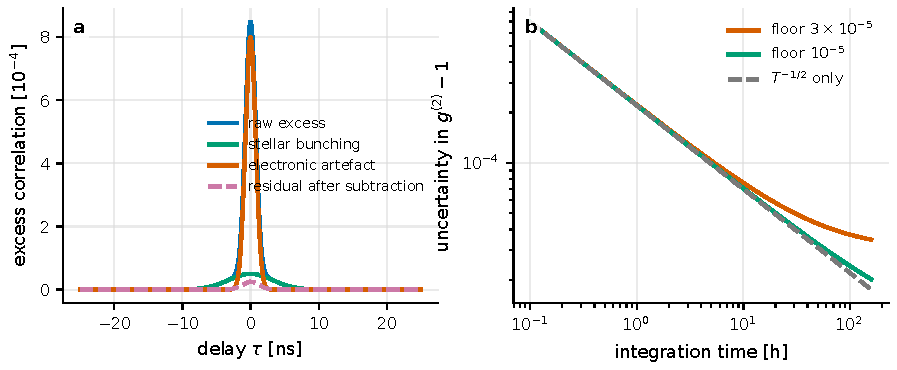
\includegraphics[width=0.96\linewidth]{figures/generated/chapter_21/ch21_calibration_artifacts.pdf}
\caption{How calibration errors disguise themselves as correlation signal. In the left panel an electronic-crosstalk peak is more than an order of magnitude above a \(5\times10^{-5}\) astronomical bunching peak; if a narrow residual remains after template subtraction, it contaminates \(\hat g^{(2)}(0)\). The right panel shows that integration time only presses down the \emph{statistical} error as \(T^{-1/2}\); once a systematic floor of \(10^{-5}\)--\(3\times10^{-5}\) exists, more integration cannot automatically improve the conclusion.}
\label{fig:e27-calibration}
\end{figure}

The correct stance against systematic terms is not ``integrate longer'' but to design a whole suite of null tests, making ``true signal'' and ``spurious signal'' behave differently under different operations: a time-shift moves one stream's events as a whole by a time far greater than the correlation width, and the true astronomical peak should vanish, while slow drift and background structure should remain; off-source or off-band switches the field or frequency band to a place without the target, and the zero-delay peak should not remain; channel permutation cross-correlates detectors, polarizations, or spectral channels that should not be correlated, and if a peak persists, suspect crosstalk first; block convergence slices the data into segments, and the mean of the correlation amplitude should be stable and the error should fall as \(T^{-1/2}\) \emph{until} it hits the floor. Guerin's report points out that if the TDC spurious correlation is not subtracted, the signal-to-noise saturates prematurely; the AQuEye/IquEye literature also explicitly lists the contributions of SPAD dead time, fiber delay, and environmental control to systematic error \citep{2017MNRAS.472.4126G,2016SPIE.9907E..0NZ,1996ApOpt..35.1956C,2013NIMPA.725..187J,2020RScI...91a3108W}.

To close: \textbf{what intensity interferometry spares you is atmospheric phase, not calibration; since the signal is diluted to }\(\mathbf{10^{-5}}\)\textbf{, one must assume instrument spurious correlations of the same order are always present, and deal with them by null tests rather than longer integration.}


\section{Why ``no phase'' does not mean ``cannot image''}
\label{sec:e27-phase}

The fourth pitfall comes from a sentence that sounds very reasonable: ``Intensity interferometry loses the phase, so it can only measure diameters, not image.'' The first half is right, the second half is wrong.

First state the right part clearly. The van Cittert--Zernike theorem of Chapter \ref{chap:e10} tells us that the angular Fourier transform of the object's brightness distribution \(I(\boldsymbol\theta)\) is the complex visibility \(V(u,v)\), which has both modulus and phase. Amplitude interferometry directly measures this complex \(V\); intensity interferometry measures the correlation of two intensity streams and obtains the modulus squared \(|V(u,v)|^2\), and \textbf{the phase of the first-order complex visibility is indeed lost}. This is a real loss of information and cannot be pretended away.

But ``losing the phase'' by no means equals ``no structure can be measured.'' \(|V|^2\) still contains a great deal of information: the diameter of a uniform disk, the degree of limb darkening, the separation and brightness ratio of a binary, the ellipticity of a rotationally flattened star, the scale of a simple disk: all can be directly fit from the dependence of \(|V|^2\) on \(u,v\). Chapter \ref{chap:e11}, in going from visibility to imaging, does exactly this. The real difficulty losing the phase brings is a specific class of \textbf{degeneracy}, the cleanest of which is the mirror degeneracy.

The reasoning of the mirror degeneracy can be laid bare in one line of algebra. Imagine reflecting the brightness distribution through a point inversion, \(I(\boldsymbol\theta)\to I(-\boldsymbol\theta)\). The Fourier transform has a basic property: if a function is point-inverted, its spectrum is complex-conjugated. Denote the complex visibility of the original brightness \(I(\boldsymbol\theta)\) as \(V(\boldsymbol u)\) (i.e.\ \(V=\widetilde I\)); then the inverted brightness \(I(-\boldsymbol\theta)\) has visibility
\[
  \mathcal V_{I(-\boldsymbol\theta)}(\boldsymbol u)
  \equiv\widetilde{I(-\boldsymbol\theta)}(\boldsymbol u)
  =V^\ast(\boldsymbol u).
\]
Taking the modulus squared,
\[
  \big|\mathcal V_{I(-\boldsymbol\theta)}(\boldsymbol u)\big|^2
  =\big|V^\ast(\boldsymbol u)\big|^2=\big|V(\boldsymbol u)\big|^2.
\]
The two are \emph{completely identical}. This means: an object and its mirror image produce the exact same \(|V|^2\), and intensity interferometry \emph{in principle} cannot separate them: the orientation information needed to separate the two is hidden precisely in the discarded sign of the visibility phase. Chapter \ref{chap:e11} already drew this phase-loss problem; Figure \ref{fig:e27-phase-loss} demonstrates it again with an unequal-brightness double source and its mirror image.

\begin{figure}[tbp]
\centering
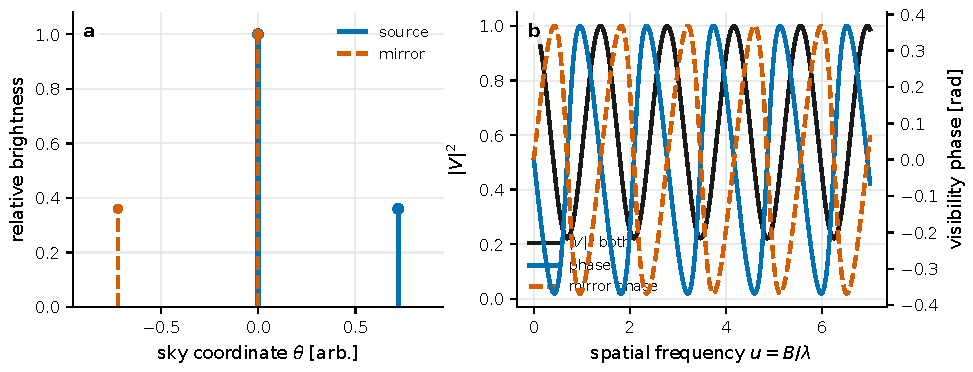
\includegraphics[width=0.96\linewidth]{figures/generated/chapter_21/ch21_phase_loss.pdf}
\caption{The mirror degeneracy from measuring only \(|V|^2\). The left panel is an unequal-brightness double source and its point-inverted mirror image; the right panel shows that the \(|V|^2\) of the two completely overlap, differing only in the sign of the visibility phase. Intensity interferometry can constrain structure, but to recover the lost orientation information one must rely on multi-baseline coverage, model priors, or higher-order correlation.}
\label{fig:e27-phase-loss}
\end{figure}

To distinguish mirror images, asymmetric structures, and complex morphologies, the correct approach is not to complain ``no phase'' but to add information: spread out multiple baselines, add physical priors, use regularized phase retrieval, or introduce higher-order information such as third-order intensity correlation \citep{2003RPPh...66..789M,2009A&A...507.1719F,2012NewAR..56..143D,2014MNRAS.437..798M,2022MNRAS.512.1722K}. The third-order correlation deserves a separate word, because it is often over-promised: ideally, third-order intensity correlation can give closure-phase-like information, thereby partially recovering orientation; but its signal is \emph{weaker} than the second-order correlation. If the statistical error of the second-order correlation is already against the systematic floor of the previous section, the third-order correlation is pinned even harder by the same photon rate and the same set of calibration problems. So third-order correlation is an exploratory direction for large arrays and extremely bright targets, while first-generation science cases (Chapter \ref{chap:e25}) are usually more pragmatic: start from few-parameter models of \(|V|^2\), then gradually add priors to build up imaging.

To close: \textbf{what intensity interferometry loses is the visibility \emph{phase}, not all structure;} \(\mathbf{|V|^2}\)\textbf{ suffices to constrain diameter, binaries, ellipticity, and many other quantities; what is truly lost is the orientation information distinguishing mirror images, to be recovered by multiple baselines, priors, or higher-order correlation.}


\section{Why quantum super-resolution cannot arbitrarily break diffraction}
\label{sec:e27-superres}

The fifth pitfall grows right beside a real achievement, so it is especially easy to fall into. SPADE (spatial-mode demultiplexing) corrects a genuine statistical misunderstanding: \textbf{the Rayleigh criterion is not the information limit of all parameter-estimation problems}. Chapter \ref{chap:e12} proved, without skipping a step: for two faint, equal-brightness, mutually incoherent point sources, when the angular separation \(s\) is far smaller than the point-spread-function width \(\sigma\), the Fisher information of direct imaging about \(s\) falls to zero as \(s^2\) (the so-called ``Rayleigh curse''), while ideal spatial-mode sorting can keep the per-photon Fisher information at a finite value \citep{2015Optic...2..646T,2016PhRvX...6c1033T,2016OExpr..24.3684N,2017PhRvL.118g0801T}. This is a true conclusion; do not discount it.

But precisely because it is true, one must all the more guard against its being exaggerated into ``quantum super-resolution can arbitrarily break diffraction, and reconstruct any complex image from a few photons.'' To see the boundary clearly, return to the Cramér--Rao bound of Chapter \ref{chap:e12}. The variance of any unbiased estimator \(\hat s\) satisfies
\begin{equation}
  \operatorname{Var}(\hat s)\;\ge\;\frac{1}{N_\gamma\,F_s},
  \label{eq:e27-crb}
\end{equation}
\begin{formulaexplain}
\(\hat s\) is the estimate of the angular separation, \(N_\gamma\) is the number of photons entering the correct mode analysis, and \(F_s\) is the Fisher information \emph{per photon} about \(s\). The measurement mode can change \(F_s\) but not \(N_\gamma\); to truly attain the bound, there must moreover be no background, aberration, or mode crosstalk.
\end{formulaexplain}

Ground each symbol. \(s\) is the angular separation to be estimated, in units of rad, mas, or directly normalized by the PSF width \(\sigma\); \(N_\gamma\) is the dimensionless effective photon number: note it is the number of photons that \emph{entered the correct mode analysis}, not the total photons hitting the telescope; \(F_s\) is the per-photon Fisher information, with dimensions of angle to the power \(-2\). Equation \eqref{eq:e27-crb} makes three things clear at once: first, what SPADE raises is \(F_s\) (blocking the \(s^2\to0\) collapse), and it \textbf{cannot substitute for }\(N_\gamma\): if the photons are too few, the variance blows up anyway; second, the bound is a ``\(\ge\),'' the \emph{best} achievable case, and \textbf{the quantum bound is not automatically attainable}: background, aberration, mode crosstalk, and centroid error each make the actual variance higher than this line; third, carrying the two-point conclusion over to an arbitrary complex image has no basis. The left of Figure \ref{fig:e27-superresolution} draws mode sorting indeed pulling the error scale far down, but a mode/centroid error floor of \(0.003\sigma\)--\(0.01\sigma\) stops the improvement; the right, with a toy model, shows that to recover higher-order moments or modes, the required photon number rises \emph{sharply}.

\begin{figure}[tbp]
\centering
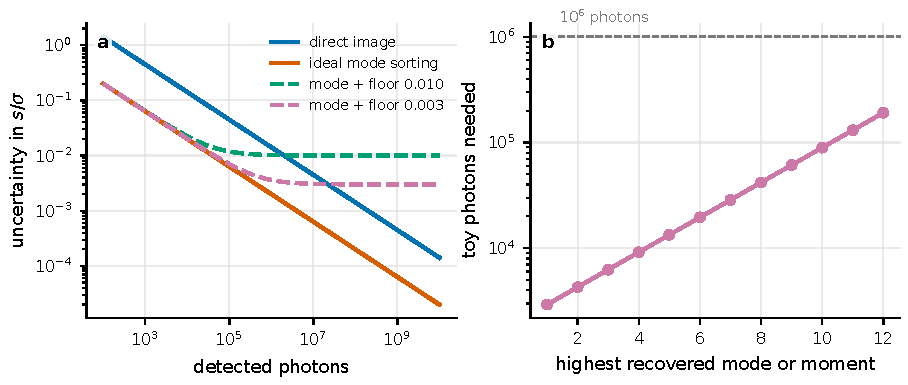
\includegraphics[width=0.96\linewidth]{figures/generated/chapter_21/ch21_superresolution_budget.pdf}
\caption{The photon budget and systematic floor of quantum super-resolution. The left panel takes \(s=0.2\sigma\) and compares the statistical-error scale of direct imaging and ideal mode sorting: mode sorting markedly lowers the error, but a mode/centroid error floor of \(0.003\sigma\)--\(0.01\sigma\) makes the improvement stop. The right panel, with a toy model, shows that the photon number required to recover higher-order moments or modes rises rapidly: a complex image cannot be arbitrarily recovered from a few photons.}
\label{fig:e27-superresolution}
\end{figure}

In the astronomical context there is a finer condition often overlooked: the coherence of the source itself, and the first-order spatial coherence after propagation. SPADE's clean conclusion is proved for ``two \emph{mutually incoherent} Gaussian point sources''; once the source is partially coherent, the mode probabilities change, and whether the Rayleigh curse reappears is precisely the condition around which the field's discussion revolves \citep{2017NJPh...19b3054T,2017PhRvA..95f3847A,2018Optic...5.1177P,2018Optic...5.1382L,2019Optic...6..400T}. Therefore, carrying the ``two incoherent Gaussian sources'' conclusion directly over to galaxies, accretion disks, jets, or strong-lensing arcs quietly discards the conditions of applicability.

To close: \textbf{the Rayleigh criterion is not the estimation limit: this is SPADE's real substance; but the quantum bound in Eq.\ }\eqref{eq:e27-crb}\textbf{ both needs sufficient }\(\mathbf{N_\gamma}\)\textbf{ and is not automatically attainable, and stripped of the conditions ``two-point, incoherent, no background, mode-aligned,'' super-resolution is only a slogan.}


\section{Where astrophysical lasers, masers, and non-Poisson statistics are most easily confused}
\label{sec:e27-maser}

The sixth pitfall centers on astrophysical stimulated-emission sources, and is several misunderstandings twisted together. The most typical line is: ``An astrophysical laser/maser must give \(g^{(2)}=1\).''

First unravel the first layer: \textbf{high brightness temperature does not equal a coherent state}. Stimulated emission can produce extremely high brightness temperature, extremely narrow spectral lines, and very strong polarization: these are the trademarks of a maser (microwave amplification by stimulated emission of radiation). But the trademark is not the intrinsic statistics. A laboratory laser approaches a coherent state by relying on a stable resonant cavity plus saturated gain to clamp the intensity fluctuations; an astrophysical environment has no such cavity at all. Chapter \ref{chap:e06} made the distinction: a coherent state is a very special quantum state, whose fingerprint is a \emph{Poisson} photon-number distribution, not ``bright'' or ``narrow.'' A spectral line that is both bright and narrow may perfectly well still carry strong intensity fluctuations: brightness temperature, line width, and polarization are measures of ``how bright, how narrow, how orderly,'' while photon statistics is a measure of ``how large the fluctuations are''; the two yardsticks measure different things. Unsaturated masers, saturated masers, velocity-coherent paths, pump fluctuations, superposition of multiple spots, and continuum background each rewrite the photon statistics \citep{1982RvMP...54.1225E,1992ARA&A..30...75E,1985ARA&A..23..169D}. In the Weigelt blobs of Eta Carinae, the natural-laser candidates of the Fe II and O I lines can be characterized only by simultaneously examining Ly\(\alpha\) pumping, level inversion, line width, spatial position, and continuum subtraction; a Brown--Twiss--Townes heterodyne correlation has even been proposed specifically to measure the line width of that extremely narrow Fe II line \citep{2004A&A...428..497J,2005MNRAS.364..731J,2005NewA...10..361J,2008AIPC..984..216D}.

The second layer is mixture dilution, worth deriving without skipping a step. Suppose the observed light is the superposition of several independent components, total intensity \(I=\sum_a I_a\), with no intensity correlation between different components. The zero-delay second-order coherence is
\[
  g^{(2)}_{\rm mix}(0)=\frac{\langle I^2\rangle}{\langle I\rangle^2}.
\]
First compute the numerator. Expand \(I^2=\big(\sum_a I_a\big)^2=\sum_a I_a^2+\sum_{a\ne b}I_aI_b\), and take the average:
\[
  \langle I^2\rangle
  =\sum_a\langle I_a^2\rangle
  +\sum_{a\ne b}\langle I_a\rangle\langle I_b\rangle,
\]
where the cross term used the assumption ``no correlation between different components,'' splitting \(\langle I_aI_b\rangle\) into \(\langle I_a\rangle\langle I_b\rangle\). Then use each component's own definition \(\langle I_a^2\rangle=g_a^{(2)}(0)\langle I_a\rangle^2\), and complete the cross sum into a full double sum minus the diagonal:
\[
  \sum_{a\ne b}\langle I_a\rangle\langle I_b\rangle
  =\Big(\sum_a\langle I_a\rangle\Big)^2-\sum_a\langle I_a\rangle^2
  =\langle I\rangle^2-\sum_a\langle I_a\rangle^2.
\]
Together:
\[
  \langle I^2\rangle
  =\sum_a g_a^{(2)}(0)\langle I_a\rangle^2
  +\langle I\rangle^2-\sum_a\langle I_a\rangle^2.
\]
Divide both sides by \(\langle I\rangle^2\), and denote the flux fraction \(f_a=\langle I_a\rangle/\langle I\rangle\):
\[
  g^{(2)}_{\rm mix}(0)
  =\sum_a g_a^{(2)}(0)f_a^2+1-\sum_a f_a^2.
\]
Move the 1 to the left, combine the right by \(f_a^2\), and obtain the clean result:

\begin{equation}
  g^{(2)}_{\rm mix}(0)-1
  =\sum_a f_a^2\left[g_a^{(2)}(0)-1\right],
  \qquad
  f_a=\frac{\langle I_a\rangle}{\sum_b\langle I_b\rangle}.
  \label{eq:e27-mixture}
\end{equation}
\begin{formulaexplain}
\(f_a\) is the flux fraction of the \(a\)-th component (dimensionless, summing to 1 over components). The crux is that \emph{square}: the correlation excess is weighted by \(f_a^2\), so a little bit of thermal continuum or multi-component mixture can scramble the reading of \(g^{(2)}\).
\end{formulaexplain}

That square is the whole crux. Plug in a number: a thermal component making up only \(20\%\) of the total flux, even if it is at full-scale \(g_a^{(2)}(0)-1=1\) on its own, contributes after mixing only \(f_a^2\times1=0.2^2=0.04\) of contrast; if this thermal component is further spread over \(M=100\) modes with \(\tau_c/\Delta t=10^{-5}\), the observed contrast becomes \(0.04\times10^{-5}/100\sim4\times10^{-9}\), completely sunk to the bottom. Conversely, an unsaturated stimulated line carrying pump intensity noise may give \emph{super}-Poisson statistics; but such a result must first cleanly separate the line, the continuum, and the instrument response, and one must never attribute \(g^{(2)}>1\) to new physics on sight. Figure \ref{fig:e27-maser} draws these two branches together.

\begin{figure}[tbp]
\centering
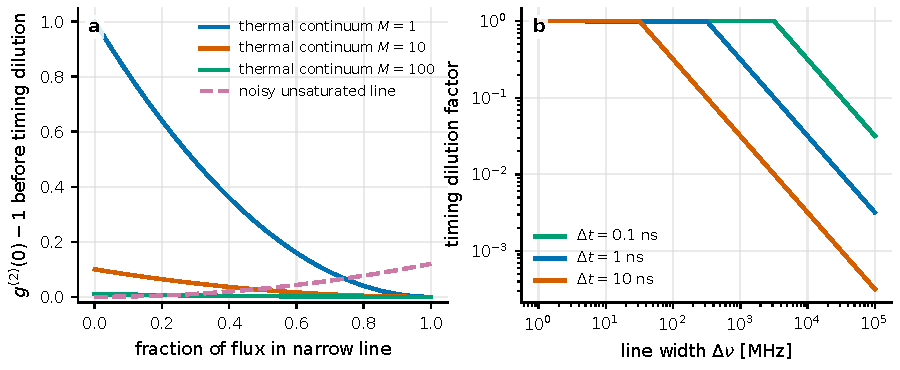
\includegraphics[width=0.96\linewidth]{figures/generated/chapter_21/ch21_maser_mixed_statistics.pdf}
\caption{Mixed statistics in astrophysical maser/laser candidates. The left panel shows that as the narrow-line flux fraction increases, the bunching of the thermal continuum is diluted by \(f_a^2\); if the narrow line itself carries unsaturated intensity noise, another super-Poisson branch emerges. The right panel shows the dilution of the correlation contrast by the line width and the electronics time bin: an MHz--GHz line width requires a ns or even faster time response to preserve an appreciable peak.}
\label{fig:e27-maser}
\end{figure}

The third layer: non-Poisson statistics have far too many \emph{ordinary} sources; do not rush to attribute them to a quantum light source. The most typical is treating a randomly variable source as a Cox process (a Cox process, also called a doubly stochastic Poisson process): given an instantaneous rate \(\Lambda\), the count is Poisson, but \(\Lambda\) itself fluctuates with time or environment. Using the law of total variance (splitting the variance into ``the expectation of the conditional variance'' plus ``the variance of the conditional expectation''), denoting \(\Lambda\) as the expected count in a bin, with Poisson conditions \(\operatorname{Var}(N\mid\Lambda)=\Lambda\) and \(\mathbb E(N\mid\Lambda)=\Lambda\), we have
\[
  \operatorname{Var}(N)
  =\mathbb E[\operatorname{Var}(N\mid\Lambda)]+\operatorname{Var}(\mathbb E[N\mid\Lambda])
  =\mathbb E(\Lambda)+\operatorname{Var}(\Lambda),
\]
while \(\mathbb E(N)=\mathbb E(\Lambda)\). Dividing the two gives the Fano factor:

\begin{equation}
  F_{\rm Fano}
  \equiv\frac{\operatorname{Var}(N)}{\mathbb E(N)}
  =1+\frac{\operatorname{Var}(\Lambda)}{\mathbb E(\Lambda)}.
  \label{eq:e27-fano}
\end{equation}
\begin{formulaexplain}
\(F_{\rm Fano}\) is the ratio of count variance to mean (equal to 1 for pure Poisson). As long as the instantaneous rate \(\Lambda\) itself fluctuates, the count naturally becomes super-Poisson (\(F>1\)), with no need to invoke a nonclassical light source at all.
\end{formulaexplain}

That is, as long as the source varies, \(F_{\rm Fano}\) at a suitable bin width is \emph{necessarily} greater than 1: the most trivial super-Poisson. The instrument also makes trouble from the opposite direction: dead time suppresses events too close together, producing negative correlation at short delays and pressing \(F_{\rm Fano}\) below 1 (under-dispersion); afterpulsing produces positive correlation after the detector's characteristic time. The afterpulsing probability of \(10^{-4}\)--\(10^{-2}\) given in Chapter \ref{chap:e07} is already enough to contaminate many short-delay searches. So before shouting ``non-Poisson,'' first draw the full set of diagnostic plots: the Fano factor versus bin width, the short-delay auto- and cross-correlation, dark-field data, off-source data, and the time-shift background. Figure \ref{fig:e27-nonpoisson} draws the different scalings of these ordinary sources side by side.

\begin{figure}[tbp]
\centering
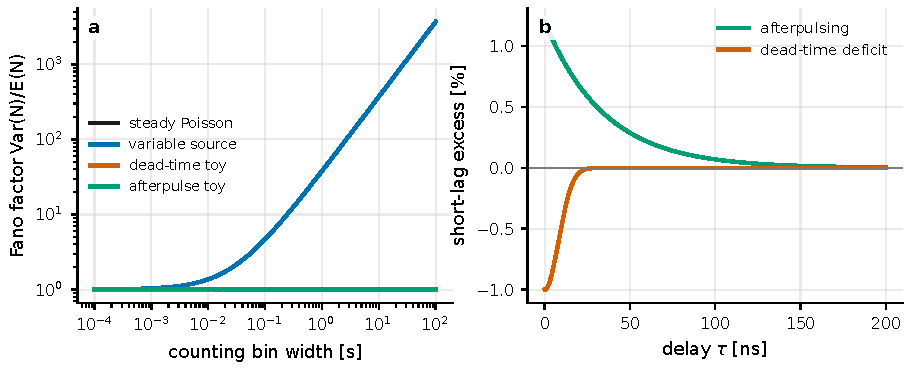
\includegraphics[width=0.96\linewidth]{figures/generated/chapter_21/ch21_nonpoisson_diagnostics.pdf}
\caption{Ordinary sources of non-Poisson statistics. The left panel uses the Fano factor to display the distinct scalings of steady-state Poisson, a slowly varying source, dead time, and afterpulsing: a slowly varying source becomes super-Poisson in long bins, and dead time causes under-dispersion. The right panel shows the opposite shapes of afterpulsing and dead time in the short-delay correlation function: these instrument features should first be quantified from dark-field and cross-channel data.}
\label{fig:e27-nonpoisson}
\end{figure}

To close: \textbf{bright, narrow, and strongly polarized do not equal a coherent state; mixed light dilutes the correlation by }\(\mathbf{f_a^2}\)\textbf{, and variable sources, dead time, and afterpulsing naturally manufacture non-Poisson statistics: before they are cleanly ruled out, no ``non-Poisson'' should be charged to new physics.}


\section{How false alarms fabricate the boundary of ``new physics''}
\label{sec:e27-false-alarm}

The last pitfall is the common ailment of all search-type work: mistaking one low-probability event for a discovery.

The root of the problem is ``multiple testing.'' Suppose the tail probability of one test giving a result this extreme by chance is \(p_0\), and you independently do \(N_{\rm trial}\) tests; then what is the probability of ``at least one'' such chance peak? Step by step: the probability of a single test \emph{not} occurring is \(1-p_0\), all \(N_{\rm trial}\) tests not occurring is \((1-p_0)^{N_{\rm trial}}\) (using independence of each), so at least one occurring is

\begin{equation}
  p_{\rm any}=1-(1-p_0)^{N_{\rm trial}}
  \simeq N_{\rm trial}\,p_0
  \qquad(N_{\rm trial}\,p_0\ll1).
  \label{eq:e27-trials}
\end{equation}
\begin{formulaexplain}
\(p_0\) is the tail probability of a single test, and \(N_{\rm trial}\) is the number of trials. The larger the search space, the higher the probability of chancing upon a high peak, so one must report the \emph{global} significance, not the single \(p_0\).
\end{formulaexplain}

That approximate equality comes from one step of standard expansion: when \(p_0\) is very small \emph{and} \(N_{\rm trial}p_0\ll1\), \((1-p_0)^{N_{\rm trial}}\approx e^{-N_{\rm trial}p_0}\approx1-N_{\rm trial}p_0\) (first using \(\ln(1-p_0)\approx-p_0\), then a first-order Taylor expansion of the exponential), and substituting back gives \(p_{\rm any}\approx N_{\rm trial}p_0\). One must remember this approximation \textbf{holds only when }\(\mathbf{N_{\rm trial}p_0\ll1}\); once the search space is so large that \(N_{\rm trial}p_0\gtrsim1\), it can no longer be used, and one must return to the un-approximated \(p_{\rm any}=1-(1-p_0)^{N_{\rm trial}}\approx1-e^{-\mu}\), where we denote
\[
  \mu\equiv N_{\rm trial}\,p_0
\]
as the \textbf{expected number} of chance peaks (dimensionless, and can be far greater than 1), while the probability \(p_{\rm any}=1-e^{-\mu}\) always lies between \(0\) and \(1\). This \(N_{\rm trial}\) can arise from all directions: the number of time bins, frequency channels, baselines, targets, model-grid points, and even windows circled out only after the fact. Plug in a number to feel it: if each night one scans \(10^6\) candidate delay/frequency/target combinations, an event with single \(p_0=10^{-5}\) (which sounds ``very significant'' already) has an expected number of chance peaks
\[
  \mu=N_{\rm trial}\,p_0\simeq10^{6}\times10^{-5}=10,
\]
so the probability of occurring globally is
\[
  p_{\rm any}=1-e^{-\mu}\approx1-e^{-10}\approx0.99995\approx1,
\]
nearly certain: meaning about \(\mu\approx10\) such ``astonishing peaks'' emerge each night on average, purely the natural tail of the search space. Here one must sharply distinguish two things: \(10\) is the expected \emph{number} \(\mu\), not a probability; writing it as \(p_{\rm any}=10\) (and casually forcing the approximation \(p_{\rm any}\approx N_{\rm trial}p_0\), which holds only for \(\mu\ll1\), onto \(\mu=10\)) is exactly the typical error this section teaches you to avoid: a probability can never exceed 1, and the quantity exceeding 1 must be the expected value of a count. The left of Figure \ref{fig:e27-false-alarm} draws a single Poisson bin with \(\mu=8\) occasionally flinging out a high-count tail of \(N\ge17\), and the right draws how the same single \(p_0\) rolls, after many trials, into a very high global false-alarm probability.

\begin{figure}[tbp]
\centering
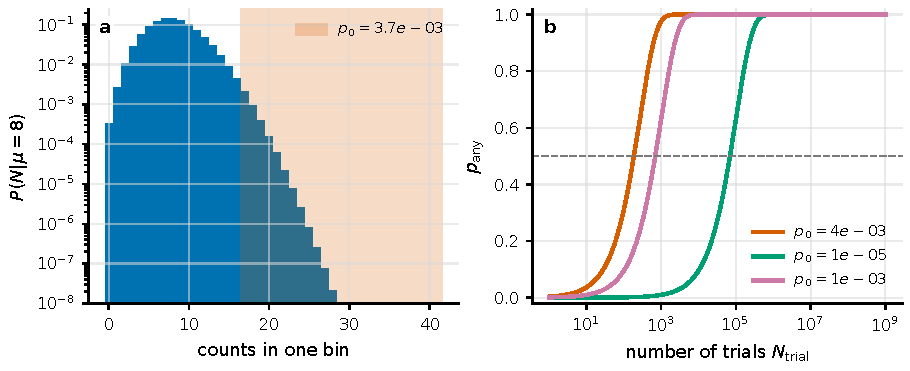
\includegraphics[width=0.96\linewidth]{figures/generated/chapter_21/ch21_poisson_false_alarm.pdf}
\caption{Poisson tails and multiple testing. In the left panel a single bin with \(\mu=8\) occasionally shows a high-count tail of \(N\ge17\); the right panel shows how the same single \(p_0\) becomes a very high global false-alarm probability over many trials. Event-table searches, period searches, cross-frequency correlations, and transient screening must all report \(N_{\rm trial}\) or the equivalent global significance.}
\label{fig:e27-false-alarm}
\end{figure}

Along the way, correct a larger semantic misunderstanding: \textbf{``quantum astronomy'' does not equal ``quantum gravity.''} The vast majority of the book so far studies light-field statistics, mode measurement, coherence functions, instruments, and information limits: all measurable ground physics. Black holes, the CMB, axions, cosmic birefringence, and dark-matter lensing can enter this main line because they can be written as \emph{observable} temporal, frequency, polarization, or spatial correlation quantities, not because each topic must invoke Planck-scale physics. The first step of a genuinely checkable anomaly is always to decompose the data sources:
\begin{equation}
  d_{\rm obs}=d_{\rm sky}(\boldsymbol\theta)
  +d_{\rm inst}(\boldsymbol\phi)
  +d_{\rm sel}(\boldsymbol\psi)
  +n.
  \label{eq:e27-data-model}
\end{equation}
\begin{formulaexplain}
\(d_{\rm obs}\) is the observed data (delay histogram, \(|V|^2\), polarization correlation, or event times); the right side separates the sky model, the instrument model, the selection function, and the noise. Any ``new physics'' explanation must first prove that these preceding ordinary terms \emph{cannot} explain the data.
\end{formulaexplain}

Here \(d_{\rm sky}(\boldsymbol\theta)\) is the object model (parameters \(\boldsymbol\theta\)), \(d_{\rm inst}(\boldsymbol\phi)\) is the instrument model, \(d_{\rm sel}(\boldsymbol\psi)\) is the selection function, and \(n\) is the noise. As long as these four terms are not yet separated, an anomalous peak, polarization rotation, or super-Poisson count should not be directly attributed to new physics; they more likely hide in \(d_{\rm inst}\) or \(d_{\rm sel}\). This connects neatly to Chapter \ref{chap:e28}: the last page of a research plan should return to ``what exactly is the new observable'': average intensity, second-order correlation, cross-frequency covariance, polarization correlation, or mode count; each quantity must come with units, typical range, and conditions of applicability (thermal light, Gaussian PSF, faint light, few-parameter source model, stable instrument response), and pick at least two null tests from time shift, off-source, off-band, dark field, wrong polarization, and injection-recovery, writing the global significance and the systematic-error floor \emph{together} into the conclusion.

To close: \textbf{the larger the search space, the more inevitable an accidental ``significant peak''; a significance that does not report }\(\mathbf{N_{\rm trial}}\)\textbf{ is meaningless, and the threshold of ``quantum astronomy'' is an observable correlation quantity, not new Planck-scale physics.}


\section{Chapter Summary}
\label{sec:e27-summary}

\begin{itemize}
  \item \textbf{Counting photons only obtains the raw material.} The real quantum information is in the joint distribution among events; if the time, detector, frequency, and polarization labels do not enter the model, even the most precise single-photon counting is still classical photometry. ``Few photons'' and ``quantum'' are two different yardsticks.
  \item \(\mathbf{g^{(2)}\simeq1}\)\textbf{ proves nothing.} The bunching peak of thermal light being diluted by the effective mode number \(M_{\rm eff}\) (including \(\Delta t_{\rm eff}/\tau_c\)) to \(10^{-5}\)--\(10^{-6}\) is the norm, see Eq.\ \eqref{eq:e27-dilution}. The only ironclad nonclassical criterion is antibunching \(g^{(2)}(0)<1\), which classical light cannot do.
  \item \textbf{Intensity interferometry does not fear phase, but fears calibration.} Since the signal is diluted to \(10^{-5}\), one must assume instrument spurious correlations of the same order are always present (Eq.\ \eqref{eq:e27-calibration-model}). The systematic floor does not fall as \(T^{-1/2}\); deal with it by null tests, not longer integration.
  \item \(\mathbf{|V|^2}\)\textbf{ loses the phase, not the structure.} Diameter, binaries, and ellipticity can all be fit; what is truly lost is the orientation information distinguishing mirror images (\(|V^\ast|^2=|V|^2\)), to be recovered by multiple baselines, priors, or higher-order correlation.
  \item \textbf{Quantum super-resolution has boundaries.} The Rayleigh criterion is indeed not the estimation limit, but the quantum bound of Eq.\ \eqref{eq:e27-crb} both needs sufficient photons \(N_\gamma\) and is not automatically attainable; away from ``two-point, incoherent, no background, mode-aligned'' it is only a slogan.
  \item \textbf{Bright, narrow, strongly polarized does not equal a coherent state.} Mixed light dilutes the correlation by \(f_a^2\) (Eq.\ \eqref{eq:e27-mixture}), and variable sources (Cox process, Eq.\ \eqref{eq:e27-fano}), dead time, and afterpulsing all naturally manufacture non-Poisson statistics: not new physics until cleanly ruled out.
  \item \textbf{A search must report global significance.} Chance peaks increase linearly with \(N_{\rm trial}\) (Eq.\ \eqref{eq:e27-trials}); an anomaly must first be decomposed into the four terms sky/instrument/selection/noise (Eq.\ \eqref{eq:e27-data-model}) before new physics can be discussed.
\end{itemize}

\medskip
\noindent\textbf{Questions to Ponder.}
\begin{itemize}
  \item You measure the thermal light of a star at \(500\,{\rm nm}\), \(5\,{\rm nm}\) bandwidth, with a \(2\,{\rm ns}\) correlation bin. In the single-mode case, what order of magnitude of \(g^{(2)}_{\rm meas}(0)-1\) do you expect to measure? (Hint: first compute \(\tau_c\), then use Eq.\ \eqref{eq:e27-dilution}.)
  \item In a spectral-line search, you find in \(3\times10^{5}\) frequency channels a peak with single \(p_0=3\times10^{-6}\). What is its global false-alarm probability? Would you declare a discovery?
  \item Someone reports \(g^{(2)}(0)=1.5\) for an astrophysical maser, claiming it is nonclassical light. Before believing it, which three ordinary sources would you first require them to rule out?
\end{itemize}

\chapter{From White Paper to Research Plan}
\label{chap:e28}

\begin{chapteropening}
By now the whole book's toolbox is full: complex amplitude and phase (Chapter \ref{chap:e01}), bandwidth and coherence time (Chapter \ref{chap:e02}), Poisson and shot noise (Chapter \ref{chap:e03}), second-order coherence \(g^{(2)}\) and the Siegert relation (Chapter \ref{chap:e08}), intensity interferometry and the van Cittert--Zernike theorem (Chapter \ref{chap:e10}), from visibility to imaging (Chapter \ref{chap:e11}), quantum estimation and SPADE (Chapter \ref{chap:e12}), event tables and clocks (Chapter \ref{chap:e13}), correlators (Chapter \ref{chap:e14}), error budgets and feasibility (Chapter \ref{chap:e15}), on to treating stars, compact stars, black holes, and transients as quantum light sources (Chapters \ref{chap:e17}--\ref{chap:e20}) and the first-generation science cases (Chapter \ref{chap:e25}). The tools are ready, but what this chapter answers is a question not so ``physical'' yet decisive of whether anything can happen at all: \textbf{how do you turn a beautiful idea into a research plan that can really be executed, and can really fail?} We walk through a clear path: \textbf{pose the science question \(\to\) select target and method \(\to\) write the error budget and estimate achievable precision \(\to\) plan the instrument and data pipeline \(\to\) lay out milestones and register risks \(\to\) write the plan}, and at each step map some formula from an earlier chapter onto an item in the proposal that can be reviewed, reproduced, and scored. The tone of this chapter turns slightly toward ``your'' next action: after reading it, you should be able to rewrite an idea into work packages, acceptance metrics, and failure criteria.
\end{chapteropening}

\section{Start from the science question: pick the right target before talking about instruments}
\label{sec:e28-question}

The most common failure in writing a plan is not ``the instrument is not good enough'' but \textbf{getting the order backward from the start}: first falling in love with an instrument or a fashionable word (``quantum,'' ``entanglement,'' ``network''), then going to look for a topic. The correct order is always: first ask a \textbf{science question} that can be observationally falsified, then ask which \textbf{observable} can answer it, and only last ask what instrument, what precision, and what kind of target source are needed.

An executable science question usually looks like this: not ``I want to study stars'' but ``just how much dimmer is the equator than the poles of this rapid rotator, and how flattened is it''; not ``I want to do quantum astronomy'' but ``are the photon statistics of this natural-laser candidate line thermal or coherent?'' The former is vague and cannot converge; the latter immediately points to an observable (the variation of \(|V|^2\) with position angle, the deviation of \(g^{(2)}(0)\) from 1) and immediately points to a set of instrument requirements.

When selecting targets, the three yardsticks of Chapter \ref{chap:e25} still apply: \textbf{brightness} decides ``whether there are photons,'' \textbf{angular scale} decides ``whether these photons can become parameters,'' and \textbf{external prior} decides ``whether the parameters can be uniquely translated into physics.'' But in writing a plan one must add one more yardstick, often overlooked in pure science discussion yet a lifeline in a proposal: \textbf{whether there is still a product after failure}. A good plan, even if the main target is not detected, should leave behind something reusable: a well-calibrated event-table format, a released version of the correlator, a calibration-star table, a set of time-synchronized null tests. Write this into target selection and you will not stake everything on a single detection that may fall through.

The product of this step is plain but is the foundation of the whole plan: a one-sentence science question + one definite observable + one ``why this target and not that'' ranking rationale. All the subsequent error budgets, instrument design, and milestones serve this one sentence. Many of the common misconceptions listed in Chapter \ref{chap:e27} (mistaking multimode thermal light for a laser, mistaking single-direction baselines for being able to determine shape, mistaking the visibility for something whose phase can be read directly) stem from \textbf{cutting corners at this step}: rushing to the instrument before thinking through ``what to measure, what can be falsified.''

\section{What can be landed in the near term: making intensity interferometry a routine data product}
\label{sec:e28-nearterm}

First the tier that \textbf{can be done now}. In the near term (the foreseeable next few years), the most mature and the most deserving of top priority for a proposal is turning the intensity interferometry already repeatedly validated by VERITAS and MAGIC from ``a single demonstration'' into ``a reproducible data product'' \citep{2020NatAs...4.1164A,2024MNRAS.529.4387A}. The quantum-network telescope is fascinating, but it belongs to a later stage (Chapter \ref{chap:e24}) and should not occupy the first batch of work packages in the near term.

The main observables of this stage are: the second-order coherence \(\hat g^{(2)}_{ab}(\tau)\), the squared visibility \(|V_{ab}|^2\), each telescope's target photon rate, the zero-baseline contrast, the background dilution factor, and the covariance on each baseline. The question is: how do we judge whether a near-term project is \textbf{actually mature}? Statements like ``the detector is available'' and ``the telescope is big enough'' cannot go into a proposal, because they cannot be accepted. We need a scorable readiness criterion.

Write the project readiness as a \textbf{ratio vector}, each entry being ``actual capability \(\div\) requirement'':
\begin{equation}
  \bm{r}=
  \left(
  \frac{R_\gamma}{R_{\rm req}},\;
  \frac{\sigma_{t,{\rm req}}}{\sigma_t},\;
  \frac{\beta_0}{\beta_{\rm req}},\;
  \frac{\sigma_{{\rm sys,req}}}{\sigma_{\rm sys}},\;
  \frac{N_{\rm cal}}{N_{{\rm cal,req}}}
  \right).
  \label{eq:e28-readiness}
\end{equation}
\begin{formulaexplain}
\(\bm r\) is the project readiness vector. Each entry is ``actual capability over requirement'': photon rate, timing precision, zero-baseline contrast, systematic-error floor, calibration sample. Only when all five entries are \textbf{simultaneously} \(\ge1\) does the near-term project close. Any entry \(<1\) is a shortfall that must be filled first.
\end{formulaexplain}
Accounting for each symbol, unit, and dimension clearly is the key to turning \eqref{eq:e28-readiness} from a ``pretty vector'' into a ``reconcilable checklist.'' \(R_\gamma\) is each telescope's effective target photon rate, units \(\mathrm{s^{-1}}\), set jointly by the collecting area, quantum efficiency, filter bandwidth, and target brightness; \(R_{\rm req}\) is the photon rate needed to reach the target precision. \(\sigma_t\) is the relative time-synchronization error between telescopes, often in ps or ns; note this entry is \textbf{requirement over capability} (\(\sigma_{t,{\rm req}}/\sigma_t\)), because the smaller the error the better, so the ``requirement'' goes in the numerator. \(\beta_0\) is the zero-baseline correlation contrast (dimensionless), measuring how much correlation signal the instrument can recover when ``two telescopes look at the same beam''; \(\beta_{\rm req}\) is the required contrast. \(\sigma_{\rm sys}\) is the residual systematic-error floor after calibration (dimensionless, same units as \(|V|^2\)), likewise entered as ``requirement over capability.'' \(N_{\rm cal}\) is the number of usable calibration stars or calibration observations, and \(N_{\rm cal,req}\) is the number required.

The value of this vector is that it \textbf{prevents a single entry from masking a shortfall}. Take a counterexample: suppose your photon rate is extremely high, \(R_\gamma/R_{\rm req}=5\), looking very abundant; but if the systematic-error floor \(\sigma_{\rm sys}=3\times10^{-5}\) is larger than the small \(|V|^2\) signal you want to measure, then \(\sigma_{\rm sys,req}/\sigma_{\rm sys}<1\), and the project is still immature: no amount of photons can flatten a systematic bias. Research on intensity-interferometry arrays stresses this repeatedly: baseline length, \(u,v\) coverage, background control, and zero-baseline calibration must all close \textbf{together}, none can be missing \citep{2006ApJ...649..399L,2013APh....43..331D,2022MNRAS.512.1722K}.

\begin{figure}[tbp]
\centering
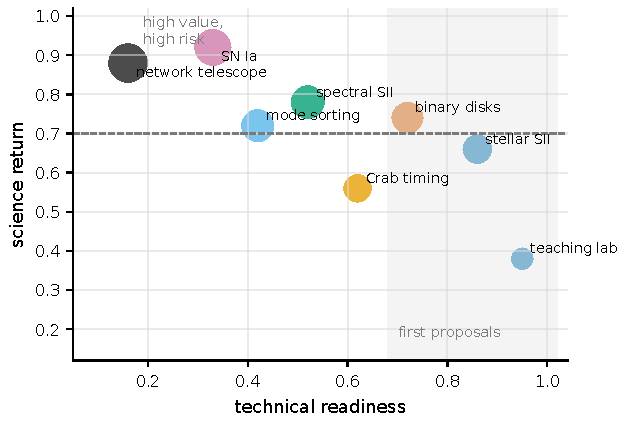
\includegraphics[width=0.86\linewidth]{figures/generated/chapter_22/ch22_roadmap_trade_space.pdf}
\caption{Technical maturity, science return, cost, and risk in the roadmap. The horizontal axis is technical maturity, the vertical axis is science return, and the larger the point, the greater the cost pressure. Tasks in the upper right with high maturity are suited to be written as near-term proposals; tasks in the upper left with high scientific value but needing a pathfinder first belong to the mid-to-far term. This figure is the visualization of the ``look at the shortfall before talking value'' approach of Eq.\ \eqref{eq:e28-readiness}.}
\label{fig:e28-trade-space}
\end{figure}

When writing a near-term plan, the more concrete the topic the better. Executable topics can be ``measure the angular diameters of 10--30 bright stars near 416 nm with four IACTs, and release the correlator and calibration library,'' or ``use the same pipeline to compare the \(|V|^2\) models of binaries, Be-star disks, and rapid rotators.'' Each paper should release: the event-table format description, the correlator version number, the time-shift null test, the calibration-star table, the baseline geometry, and the posterior samples. This way, even if some targets are not detected, reusable instrument knowledge is left behind, exactly the ``product after failure'' of the previous section.

\section{Error budget and feasibility: first estimate the precision you can reach}
\label{sec:e28-budget}

The item most indispensable in a plan, and the first thing a referee looks at, is the \textbf{error budget}: the core tool of Chapter \ref{chap:e15}. It answers two questions: ``How accurately can this observation ultimately measure the observable?'' ``Is it statistical noise, or some systematic error, that limits this precision?'' A proposal without an error budget is like saying ``I want to do it, but I don't know how well I can do it,'' and is almost certain to be rejected.

The skeleton of an error budget is to \textbf{add in quadrature} the various independent errors. Why add in quadrature rather than directly? Because for several \textbf{mutually independent} random errors, the total variance equals the sum of the individual variances (a direct consequence of the additivity of variances of independent random variables in probability theory, covered in Chapter \ref{chap:e03}). Let the standard deviations of the error sources be \(\sigma_{\rm stat},\sigma_{\rm cal},\sigma_{\rm bg},\sigma_{\rm model},\sigma_{\rm sel}\); then the total error is
\begin{equation}
  \sigma_{\rm tot}^2
  =
  \sigma_{\rm stat}^2
  +\sigma_{\rm cal}^2
  +\sigma_{\rm bg}^2
  +\sigma_{\rm model}^2
  +\sigma_{\rm sel}^2 .
  \label{eq:e28-error-budget}
\end{equation}
\begin{formulaexplain}
Each term is the standard deviation of one error source's contribution to the final observable (same dimensions as the observable): \(\sigma_{\rm stat}\) statistical, \(\sigma_{\rm cal}\) calibration, \(\sigma_{\rm bg}\) background, \(\sigma_{\rm model}\) model, \(\sigma_{\rm sel}\) selection effect. Independent errors add in variance, so \textbf{the largest term dominates the total error}: go press that one down first.
\end{formulaexplain}
Grounding each term, and also explaining where each comes from. \(\sigma_{\rm stat}\) is statistical noise, from the finite sample of Poisson or correlated counts, falling as \(T^{-1/2}\) with integration time. \(\sigma_{\rm cal}\) is calibration error, from imperfections in zero-baseline contrast, time synchronization, and polarization and spectral response. \(\sigma_{\rm bg}\) is background, from night-sky light, continuum, or companion-star blending. \(\sigma_{\rm model}\) is model error, from the stellar disk, supernova photosphere, BLR, or maser geometry you use to fit being itself insufficiently realistic. \(\sigma_{\rm sel}\) is selection effect, from biases introduced by triggering, weather, and target selection. The practical reading of Eq.\ \eqref{eq:e28-error-budget} is: \textbf{adding in quadrature means the largest term has a veto}: if one term is three times larger than the rest, the others after square-rooting barely change the total, and all your effort should go to cutting that one term. Statistical tools like MCMC, nested sampling, or posterior predictive checks can help you compute \(\sigma_{\rm stat}\) and the parameter posterior accurately, but they \textbf{cannot substitute for} the physical error terms \(\sigma_{\rm cal}\), \(\sigma_{\rm model}\) themselves \citep{2013PASP..125..306F,2009MNRAS.398.1601F,1979ApJ...228..939C,2013ApJ...764..167S}.

The term one should estimate first in the error budget is often the statistical term \(\sigma_{\rm stat}\), because it directly tells you ``whether this target is doable at all.'' The intensity-interferometry signal-to-noise given in Chapter \ref{chap:e15} is a known result that can be used by name (Hanbury Brown's classic expression):
\begin{equation}
  \left(\frac{S}{N}\right)
  =
  A\,\alpha\,n\,|V|^2
  \sqrt{\frac{\Delta f\,T}{2}} .
  \label{eq:e28-snr}
\end{equation}
\begin{formulaexplain}
The signal-to-noise of intensity interferometry: \(A\) collecting area, \(\alpha\) quantum efficiency, \(n\) the spectral photon flux per unit area per unit bandwidth (spectral flux density), \(|V|^2\) the squared-visibility signal, \(\Delta f\) the electronic bandwidth, \(T\) the integration time. The crux is that the signal-to-noise grows only as \(\sqrt{T}\): to double the precision, the integration time must quadruple.
\end{formulaexplain}
Laying out the units of the symbols: \(A\) has units \(\mathrm{cm^2}\), \(\alpha\) is dimensionless (typically \(0.2\text{--}0.3\)), \(n\) has units \(\mathrm{cm^{-2}\,Hz^{-1}\,s^{-1}}\) (also understandable as the photon occupation per mode per second \(\bar n_\nu\) times a geometric factor, see Chapter \ref{chap:e15}), \(\Delta f\) has units Hz, and \(T\) has units s. Hidden in this equation are three intuitions that must be internalized when writing a plan: first, the signal is \(|V|^2\) rather than \(|V|\): once the target is partially resolved and \(|V|^2\) drops, the signal-to-noise loses \textbf{by the square}, which is why the angular scale must match the baseline. Second, the signal-to-noise grows only as \(\sqrt{\Delta f\,T}\): raising the precision to double costs four times the observing time or four times the electronic bandwidth, and this \(\sqrt{\cdot}\) law directly sets your requested duration. Third, \(n\) depends on wavelength and bandwidth, and the appeal of spectral multiplexing is precisely that it can accumulate this SNR in parallel across many channels (next section).

Plug in a set of real numbers to land the feasibility. Take a pair of \(100\,\mathrm{m^2}\) telescopes (i.e.\ \(A=10^6\,\mathrm{cm^2}\)), quantum efficiency \(\alpha=0.25\), electronic bandwidth \(\Delta f=200\,\mathrm{MHz}=2\times10^8\,\mathrm{Hz}\), integration time \(T=5\,\mathrm{h}=1.8\times10^4\,\mathrm{s}\). Here the order of magnitude most easily misestimated is the dimensionless combination \(A\alpha n\): substituting \(A=10^6\,\mathrm{cm^2}\), \(\alpha=0.25\), and a spectral photon flux of about \(n\sim4\times10^{-11}\,\mathrm{cm^{-2}\,Hz^{-1}\,s^{-1}}\) for an \(m_V\simeq6\) hot star in a narrow band, we get \(A\alpha n\sim10^{-5}\). Note in particular that this number is \textbf{far less than 1}: it is in fact the degeneracy parameter of thermal light, that is, the order of magnitude of the photon occupation per mode per second \(\bar n_\nu\) times a geometric factor; precisely because the \(\bar n_\nu\ll1\) of a visible-light thermal star, the intensity-interferometry signal is so weak and so hard to obtain (which is also why one must scrape it together with large area and long integration). Take the signal on a representative baseline where the source is partially resolved, \(|V|^2\sim0.5\) (at the true zero baseline \(|V|^2\to1\); here we have already left the zero baseline by some amount and the source is partially resolved). Then \(\sqrt{\Delta f\,T/2}=\sqrt{2\times10^8\times1.8\times10^4/2}=\sqrt{1.8\times10^{12}}\approx1.3\times10^6\), so \(S/N\sim10^{-5}\times0.5\times1.3\times10^6\approx6.7\), that is, of order a few sigma, consistent with the estimate of LeBohec and Holder that ``a several-sigma detection of an \(m_V\simeq6.7\) source can be made within 5 hours'' for the present generation of instruments \citep{2006ApJ...649..399L,2013APh....43..331D}. Conversely, if the target is 1 magnitude fainter, the photon flux \(n\) drops to about \(40\%\), and in the same time the signal-to-noise drops to about \(40\%\); to make it back one must raise \(T\) to about \(6\) times; such numbers must be written into the feasibility subsection of the proposal, not vaguely stated as ``we believe it can be done.''

\section{Instrument and data pipeline: from event table to public archive}
\label{sec:e28-pipeline}

Having estimated the precision, one must next answer ``what instrument and what data pipeline will realize this precision.'' This section pushes the plan from ``how accurately can it be measured'' to ``how to measure it, what the data look like, and how others reproduce it.''

The data product of a near-term project is still simple: one blue-filter \(|V|^2\) plus the covariance of a few baselines. But a far-sighted plan should plan how the \textbf{data product will grow}. The mid-term goal is to expand ``single-channel \(|V|^2\)'' into a \textbf{multi-channel event table}: spectrally resolved intensity interferometry can compare the angular scales inside and outside spectral lines (the disk is larger than the photosphere, and the \(|V|^2\) of the line region falls faster); polarization-resolved correlation can examine the magnetic-field geometry, scattering, and strong-field radiation; picosecond-level event tables can treat the photon statistics themselves as a new time-domain data product. The appeal of spectral multiplexing is that each spectral channel has a longer coherence time, and multiple channels can accumulate the signal-to-noise of Eq.\ \eqref{eq:e28-snr} in parallel; the price is that the data rate, inter-channel calibration, and dispersion model all become more complex \citep{2021sf2a.conf..335L,2022MNRAS.512.1722K,2024MNRAS.529.4387A}.

Writing the data product of the multi-channel stage as a set is when the plan enters engineering language:
\begin{equation}
  \bm{d}=
  \left\{
  H_{ab}^{\nu p}(\tau),\;
  \widehat{|V_{ab}^{\nu p}|^2},\;
  C_{\nu_i\nu_j}^{p_i p_j},\;
  \bm{\Sigma}
  \right\}.
  \label{eq:e28-data}
\end{equation}
\begin{formulaexplain}
\(\bm d\) is the complete data product of the multi-channel stage, not just \(|V|^2\): \(H_{ab}^{\nu p}(\tau)\) is the delay histogram, \(\widehat{|V_{ab}^{\nu p}|^2}\) is the calibrated squared visibility, \(C_{\nu_i\nu_j}^{p_i p_j}\) is the cross-frequency/cross-polarization covariance, and \(\bm\Sigma\) is the covariance matrix binding these quantities together. \textbf{How the data are stored, normalized, and released} determines whether the project has reached the engineering stage.
\end{formulaexplain}
Explaining the meaning and role of each term. \(H_{ab}^{\nu p}(\tau)\) is the coincidence-count histogram at telescope pair \(a,b\), frequency channel \(\nu\), polarization channel \(p\), and delay \(\tau\): it is the raw product the correlator (Chapter \ref{chap:e14}) directly spits out, and \(\hat g^{(2)}\) is its normalized shape. \(\widehat{|V_{ab}^{\nu p}|^2}\) is the spatial-coherence observable calibrated from the histogram (the van Cittert--Zernike bridge of Chapter \ref{chap:e10} connects it to the source's angular structure). \(C_{\nu_i\nu_j}^{p_i p_j}\) is the covariance between different frequency or polarization channels, carrying the ``genuinely new'' physics of the angular-scale contrast inside versus outside spectral lines and between different polarizations. \(\bm\Sigma\) is the covariance matrix of the whole dataset, which must be used when fitting object parameters, rather than pretending the points are independent. Writing merely one sentence ``we will do multi-channel quantum observation'' is far from enough; writing clearly the storage format, normalization convention, and release method of each quantity in \(\bm d\) is an engineering-grade plan.

\begin{figure}[tbp]
\centering
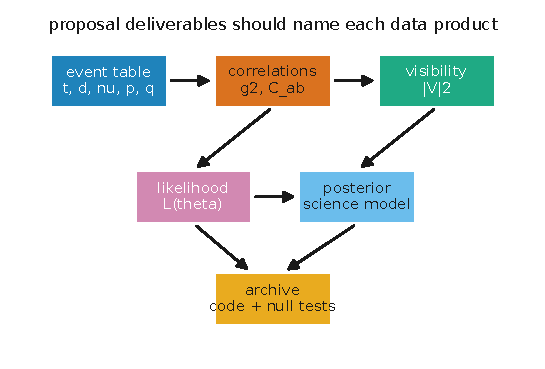
\includegraphics[width=0.88\linewidth]{figures/generated/chapter_22/ch22_data_product_stack.pdf}
\caption{The product chain from proposal to public data. The event table retains each photon's arrival time, telescope, frequency, polarization, and quality flag; the correlator turns it into \(g^{(2)}\) and covariance; the spatial model gives \(|V|^2\); the likelihood and posterior connect it to object parameters; and the archive layer must include the code, version numbers, and null tests. Each quantity in Eq.\ \eqref{eq:e28-data} corresponds to one link in this chain.}
\label{fig:e28-data-products}
\end{figure}

When planning the data pipeline, there is a principle running through the whole book worth writing on the plan's first page: \textbf{the event table is the common language}. Whether it is a classroom tabletop HBT demonstration (Chapter \ref{chap:e26}), a small-aperture pathfinder, or a large-facility observation, they can all share the same ``arrival time + telescope + frequency + polarization + quality flag'' event-table format and the same version of correlator \citep{2016SPIE.9907E..0NZ,2025MNRAS.537.2527M}. This means the data format you define in the plan lets teaching, pathfinder, and main facility connect seamlessly, which is itself a design that lowers risk and raises reproducibility.

\section{Risks and milestones: let the plan fail, but fail with value}
\label{sec:e28-risk}

A plan that writes only ``what we will do and what we expect to see'' is in fact not yet ready to face reality. In reality the target will be fainter than expected, the systematic error will stick at some floor, and the transient will trigger too late. A mature plan must proactively write out \textbf{milestones} (breaking success into acceptable nodes) and a \textbf{risk register} (listing where things may go wrong together with mitigation plans).

First the milestones. An executable milestone must \textbf{simultaneously} specify ``what to measure'' and ``what counts as success,'' otherwise it is only a vision. Write it as a quintuple:
\begin{equation}
  m_j=
  \left(
  O_j,\;
  \sigma_{O,j}^{\rm goal},\;
  T_j,\;
  N_{{\rm null},j},\;
  D_{{\rm release},j}
  \right).
  \label{eq:e28-milestone}
\end{equation}
\begin{formulaexplain}
\(m_j\) is the \(j\)-th milestone: \(O_j\) is the observable to be measured, \(\sigma_{O,j}^{\rm goal}\) is the target precision to be reached, \(T_j\) is the completion date or observing time needed, \(N_{{\rm null},j}\) is the number of null tests that must be passed, and \(D_{{\rm release},j}\) is the data product to be released. A milestone that \textbf{simultaneously pins down} observable, precision, time, verification, and delivery keeps the roadmap from stalling at slogans.
\end{formulaexplain}
Grounding each term and giving typical values. \(O_j\) is the observable, for example \(g^{(2)}(0)-1\), \(|V|^2\), the angular-scale ratio inside versus outside a line, or the distance \(D_A\). \(\sigma_{O,j}^{\rm goal}\) is the target precision, coming directly from the error budget \eqref{eq:e28-error-budget} of the previous section: a milestone's precision goal cannot be pulled out of thin air but must be a number the error budget computes. \(T_j\) is the completion date or the machine time required. \(N_{{\rm null},j}\) is the number of null tests: a near-term project can require \(N_{\rm null}\ge2\) (time-shift and off-source); a mid-term multi-channel project should rise to \(N_{\rm null}\ge4\) (adding off-band, wrong-polarization, injection-recovery); and a far-term network project must further include independent acceptance of link fidelity and storage decoherence. \(D_{{\rm release},j}\) is the delivered data product, for example some subset of Eq.\ \eqref{eq:e28-data} plus the code and version numbers. Writing all five items lets a review judge, item by item, which node has passed and which still owes.

\begin{figure}[tbp]
\centering
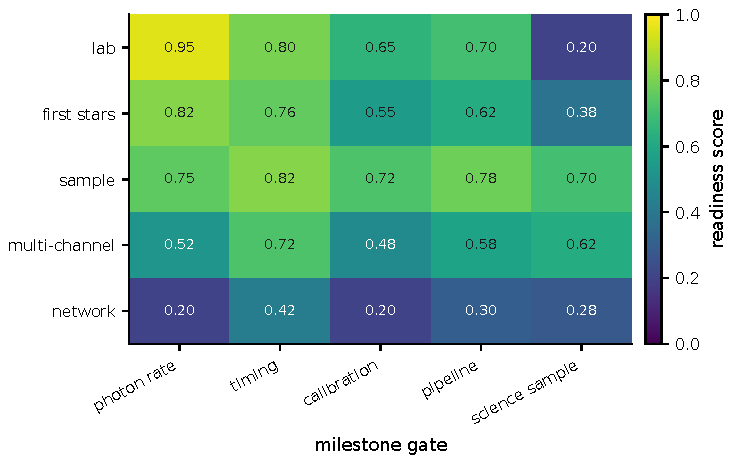
\includegraphics[width=0.90\linewidth]{figures/generated/chapter_22/ch22_milestone_gates.pdf}
\caption{The milestone-gate matrix for different stages. Course experiments and first-generation stellar intensity interferometry are already fairly mature in photon rate, timing, and pipeline, but multi-channel calibration and the network stage still have clear gaps. The numbers in the figure are only \emph{examples} of the readiness scores a proposal should explicitly quantify, used to illustrate how each item of Eq.\ \eqref{eq:e28-milestone} should be scored, and do not represent any facility commitment.}
\label{fig:e28-gates}
\end{figure}

Now the risks. The essence of a risk register is to bind each risk to a \textbf{failure criterion}: not only saying ``what may go wrong'' but also ``at what degree one should change the plan, and change it to what.'' Several concrete examples, all quantifiable by the earlier formulas: if the target star is 1 mag fainter than expected, then by Eq.\ \eqref{eq:e28-snr} the photon flux drops and the signal-to-noise falls to about \(40\%\): the mitigation is to prepare brighter backup targets in advance or extend the machine time. If the systematic-error floor stalls at \(\sigma_{\rm sys}\sim3\times10^{-5}\), then by Eq.\ \eqref{eq:e28-error-budget} many small \(|V|^2\) signals are drowned by this term: the mitigation is to build a calibration-star library first to press \(\sigma_{\rm cal}\) down. If a Type Ia trigger is 10 days late, the shell is larger but the luminosity has already fallen and the model uncertainty \(\sigma_{\rm model}\) rises: the mitigation is to write the trigger response as a hard metric and set a clear abandonment criterion for late-arriving events. If the quantum-network link gives only very few high-fidelity entangled pairs per day, the science mode should \textbf{fall back} to local mode sorting or ordinary intensity interferometry, rather than forcing the network scheme (Chapter \ref{chap:e24}).

\begin{figure}[tbp]
\centering
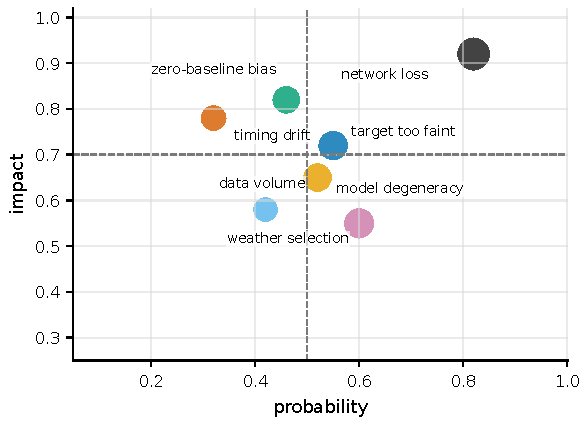
\includegraphics[width=0.86\linewidth]{figures/generated/chapter_22/ch22_risk_register.pdf}
\caption{The roadmap's risk-register figure. The horizontal and vertical axes are occurrence probability and impact, and the larger the point, the weaker the existing mitigation. Risks in the upper-right corner must have mitigations in place before the project begins: network loss needs a short-baseline pathfinder first, zero-baseline bias needs a calibration-star library first, and an over-faint target needs preset clear trigger and abandonment criteria.}
\label{fig:e28-risk}
\end{figure}

These two things together convey perhaps the most important attitude of this chapter: \textbf{a good research plan allows itself to fail, but makes every failure tell the next stage what to change}. A night with zero detections, as long as it leaves behind a well-calibrated event table, passed null tests, and a released version of the correlator, has advanced the instrument knowledge one step, far better than a plan that ``reports only successes.''

\section{Weaving the whole book into a path: from course project to research topic}
\label{sec:e28-path}

Finally, twist the six preceding steps into one rope, and see how it grows from a classroom exercise all the way into a submittable research plan, and where along this path far-term ideas like the quantum network should be placed.

The starting point can be very small. The course project (Chapter \ref{chap:e26}) begins with tabletop HBT, event-table simulation, uniform-disk fitting, the Fisher information of SPADE (Chapter \ref{chap:e12}), and false-alarm calculation: these exercises look like toys, yet they already walk a miniature version of the path ``pose the question \(\to\) design the observation \(\to\) estimate the precision \(\to\) write the plan.'' One level up, a smaller research topic is well suited to revolve around \textbf{one pipeline}: time synchronization, correlator, calibration library, target sample, or an open-data notebook: each can stand as its own paper and each leaves behind a reusable product. Higher still, a fuller science topic can aim at the line angular scale of a Be-star \(\mathrm{H}\alpha\) disk, the multi-baseline model of a rapid rotator, the phase-resolved photon statistics of the Crab pulsar, the systematic errors of a Type Ia distance toy model, or a joint experiment of local mode sorting (Chapter \ref{chap:e12}) with adaptive optics. At the top level, a large collaboration then connects these topics to CTAO/IACT, ELT/VLTI/CHARA, Rubin, SKA, gravitational-wave networks, and even quantum-network laboratories.

Regarding the \textbf{far term}: when the quantum-network telescope becomes the main line, the plan must honestly stratify. Many information-theoretic benefits do not require a complete quantum network: local mode sorting and phase-sensitive measurement (Chapter \ref{chap:e12}) can already improve the information efficiency of small-separation and brightness-moment estimation, and this can be advanced \textbf{now} \citep{2016PhRvX...6c1033T,2017PhRvL.118g0801T}. Two-photon astrometry, single-photon-assisted or linear-optics pathfinders aim to stably couple astronomical light with laboratory quantum resources, and belong to the mid-term \citep{2023PhRvL.130p0801M,2024SPIE13095E..1NR}. True entanglement-assisted long-baseline interferometry requires the entanglement-distribution rate, quantum storage time, frequency-conversion efficiency, Bell fidelity, and astronomical synchronization to meet their targets \textbf{simultaneously}, and belongs to a later stage \citep{2025PhRvA.111d3701M,2026PhRvA.113a2608P}. This resource threshold has already been written in Chapter \ref{chap:e24} as constraints on link rate, storage time, and effective fidelity; in writing a plan one need only remember one order of magnitude: at baseline \(B=1000\,\mathrm{km}\) the light-travel time is \(B/c\simeq3.3\,\mathrm{ms}\), and a ground-based km-scale baseline needs only \(\mu\mathrm{s}\)-to-ms-level synchronization, but a global or space baseline rapidly amplifies the storage and distribution pressure. If any one of link loss, storage decoherence, or useful photon rate fails to meet its target, the network scheme is not yet sufficient to replace ordinary intensity interferometry, and at that point an honest plan should fall back to the tier that can be done in the near term, rather than overdrawing the future in the proposal.

\begin{figure}[tbp]
\centering
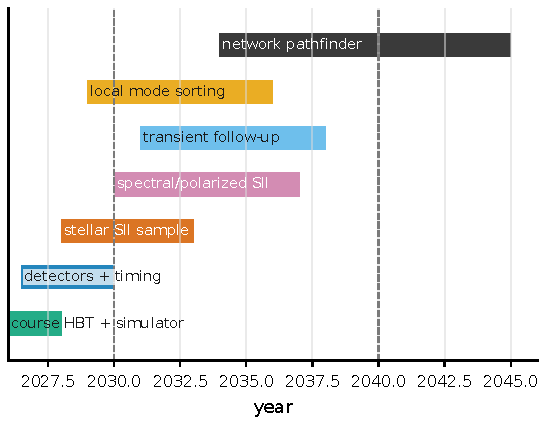
\includegraphics[width=0.92\linewidth]{figures/generated/chapter_22/ch22_program_timeline.pdf}
\caption{The staged timeline from course HBT to quantum-network pathfinder. Early tasks build talent, event tables, timing, and calibration; mid-term tasks produce the first-generation science sample and multi-channel correlation; far-term tasks should be written as facility-level roadmaps only after local mode sorting, link, and storage metrics meet their targets. This timeline is precisely the path of this chapter, ``growing from a course project into a research topic.''}
\label{fig:e28-timeline}
\end{figure}

Compress all of this into one operational acceptance standard: \textbf{a qualified research plan must at minimum list the new observables, the event-table fields, the data-estimation steps, the units and typical ranges of each symbol, two or more null tests, and the data, code, or instrument constraints that will remain even after failure}. Meet these, and your plan can be reproduced, reviewed, and improved; otherwise the word ``quantum'' stays only in the title, landing on no falsifiable number. This is precisely the last thing the whole book wants to teach you: turn tools into questions, turn questions into observations, and turn observations into a plan that others can carry forward.

\section*{Chapter Summary}
\addcontentsline{toc}{section}{Chapter Summary}

\begin{itemize}
  \item \textbf{The order cannot be reversed.} First pose the science question, then fix the observable, and only last talk about instruments and precision. Beyond brightness, angular scale, and external prior, target selection must ask one more thing: ``Is there still a product after failure?''
  \item \textbf{Maturity must be acceptable.} Use the ratio vector \eqref{eq:e28-readiness} to score a near-term project: photon rate, timing, zero-baseline contrast, systematic error, and calibration sample must \textbf{simultaneously} meet their targets, and any entry \(<1\) is a shortfall that must be filled first.
  \item \textbf{The error budget is the foundation.} Independent errors add in variance (Eq.\ \eqref{eq:e28-error-budget}), and the largest term has a veto; statistical noise can be estimated by Eq.\ \eqref{eq:e28-snr}, the signal-to-noise grows only as \(\sqrt{\Delta f\,T}\), doubling the precision costs quadruple machine time, and this must be written into the feasibility subsection (Chapter \ref{chap:e15}).
  \item \textbf{The data pipeline must be engineered.} Write the data product as a set \eqref{eq:e28-data}: delay histogram, \(|V|^2\), cross-channel covariance, and full covariance matrix; define the format well so that teaching, pathfinder, and main facility can share the same event table (Chapters \ref{chap:e13}, \ref{chap:e14}).
  \item \textbf{Milestones and risks are written together.} The milestone quintuple \eqref{eq:e28-milestone} simultaneously pins down observable, precision, time, number of null tests, and delivery; risks must be written together with failure criteria, letting the plan fail, but fail in a way that tells the next stage what to change.
  \item \textbf{The far term must be honestly stratified.} Local mode sorting can be done now, the pathfinder is mid-term, and the entanglement-assisted network is the main line only when several metrics meet their targets simultaneously (Chapter \ref{chap:e24}); if they do not, honestly fall back to the tier that can be done in the near term.
\end{itemize}

\medskip
\noindent\textbf{Questions to Ponder}
\begin{itemize}
  \item You hold a readiness vector \eqref{eq:e28-readiness} in which the photon-rate entry is \(R_\gamma/R_{\rm req}=4\) and the other four entries are all around \(0.9\). Should this project be written as a proposal now? If not, into which entry would you first invest machine time and funds?
  \item Use Eq.\ \eqref{eq:e28-snr} to estimate: if the electronic bandwidth \(\Delta f\) is raised from \(200\,\mathrm{MHz}\) to \(800\,\mathrm{MHz}\), with all else unchanged, to roughly what fraction of the original is the integration time needed to reach the same signal-to-noise shortened?
  \item Pick a science case from Chapter \ref{chap:e25} for yourself, and try to write it as a milestone quintuple \eqref{eq:e28-milestone}: what should its \(O_j\), \(\sigma_{O,j}^{\rm goal}\), \(N_{{\rm null},j}\), and \(D_{{\rm release},j}\) be filled with? Which item can you not yet answer, and what step does that tell you the plan still lacks?
\end{itemize}


% ------------------------------------------------------------
\appendix
\chapter{Index of Common Formulas}
\label{app:a}

This formula index lists where each relation first appears in a settled form. When a later chapter needs the same set of quantities, return here and to the corresponding place in the main text first to check symbols, units, orders of magnitude and conditions of validity.

\section{Event Tables, Counts and Likelihoods}
\label{appsec:a-observables}

\begin{longtable}{p{0.22\linewidth}p{0.31\linewidth}p{0.37\linewidth}}
\toprule
Topic & Location & Check when using \\
\midrule
Photon event-table fields & Chapter~\ref{chap:e00}; instrument-level extensions in Chapter~\ref{chap:e13} & Time reference, detector or telescope index, frequency channel, polarization, quality flags, spatial pixel and weight. \\
Time calibration & Chapter~\ref{chap:e13} & Raw TDC time, clock drift, optical-path delay, barycentric correction and absolute synchronization. \\
Poisson counts & Chapter~\ref{chap:e00} & Whether the expected count includes source variability, background, exposure, selection function and dead time. \\
Unbinned point-process likelihood & Chapter~\ref{chap:e14} & Whether event times are preserved; whether the rate model varies with time, energy or quality window. \\
Binned Poisson likelihood & Chapter~\ref{chap:e14}; pedagogical projection in Chapter~\ref{chap:e26} & Whether the bin width is appropriate relative to the physical time scale, the instrument response and the statistical count requirement. \\
Delay and pair count & Chapter~\ref{chap:e14} & Delay window, time-shift background, accidental coincidences, duplicate events and quality selection. \\
\(g^{(2)}\) estimator & Chapter~\ref{chap:e14} & Normalization, background window, width of the zero-delay peak and uncorrelated-channel checks. \\
Covariance and posterior & Chapter~\ref{chap:e14} & Whether the data points are correlated; whether the prior and likelihood are written on the same data vector. \\
\bottomrule
\end{longtable}

\section{Coherence, Visibility and Intensity Interferometry}
\label{appsec:a-coherence}

\begin{longtable}{p{0.22\linewidth}p{0.31\linewidth}p{0.37\linewidth}}
\toprule
Topic & Location & Check when using \\
\midrule
Complex visibility & Chapter~\ref{chap:e10} & Angular-coordinate units, projected baseline, wavelength, narrow-field approximation, bandwidth averaging and source model. \\
Uniform disk & Chapter~\ref{chap:e10} & Whether the angular diameter is a radius or a diameter; whether limb darkening is needed; whether the baseline reaches near the first null. \\
Siegert relation & Chapter~\ref{chap:e08}; spatial HBT in Chapter~\ref{chap:e10} & Whether the thermal-light, chaotic-light or Gaussian-field approximation holds; whether polarization, spectrum and number of modes change the contrast. \\
Intensity-interferometry observation model & Chapter~\ref{chap:e10}; calibration model in Chapter~\ref{chap:e27} & Whether zero-baseline contrast, peak shape, instrumental crosstalk, selection function and statistical noise are kept separate. \\
Coherence time & Chapter~\ref{chap:e08}; instrument-channel form in Chapter~\ref{chap:e13} & Filter bandwidth, line width, central wavelength and frequency units. \\
Contrast dilution & Chapter~\ref{chap:e08} & Electronic response, correlation bin, effective number of modes, polarization averaging and spectral averaging. \\
Background dilution & Chapter~\ref{chap:e13} & Target flux fraction, night-sky brightness, companion stars, line-to-continuum ratio, dark counts and calibrator stars. \\
Intensity-interferometry SNR & Chapter~\ref{chap:e10}; observational feasibility in Chapter~\ref{chap:e15} & Photon rate, telescope area, integration time, equivalent bandwidth, \(|V|^2\) and the systematic-error floor. \\
Number of baselines & Chapter~\ref{chap:e10} & Adding telescopes increases the number of correlation tasks quadratically; data rate and calibration complexity rise in step. \\
\bottomrule
\end{longtable}

\section{Instrument Response and Data Rates}
\label{appsec:a-instrument}

\begin{longtable}{p{0.22\linewidth}p{0.31\linewidth}p{0.37\linewidth}}
\toprule
Topic & Location & Check when using \\
\midrule
Data rate & Chapter~\ref{chap:e13} & Sampling time, number of bits, number of spectral channels, number of telescopes and real-time correlator capacity. \\
Response convolution & Chapter~\ref{chap:e13} & The response kernel formed jointly by the detector pulse, cabling, amplifier, digitizer and software correlation window. \\
Jitter budget & Chapter~\ref{chap:e13} & Detector jitter, clock synchronization, fiber delay, trigger jitter and barycentric correction. \\
Event-table quality selection & Chapters~\ref{chap:e14} and~\ref{chap:e26} & Clouds, saturation, events near dead time, anomalous background, bad channels and target altitude. \\
Decomposition of calibration terms & Chapter~\ref{chap:e27} & Astrophysical terms, instrumental terms, selection-function terms and random errors must not be mixed into a single free constant. \\
\bottomrule
\end{longtable}

\section{Estimation Theory and Mode Measurement}
\label{appsec:a-estimation}

\begin{longtable}{p{0.22\linewidth}p{0.31\linewidth}p{0.37\linewidth}}
\toprule
Topic & Location & Check when using \\
\midrule
Fisher information & Chapter~\ref{chap:e14}; spatial-mode example in Chapter~\ref{chap:e12} & Whether the parameters, data vector, covariance, derivatives and prior match the actual observation. \\
Cramér--Rao lower bound & Chapter~\ref{chap:e12} & The bound is a result under local, unbiased or asymptotic conditions; systematic errors are not automatically included. \\
Quantum Fisher information for a Gaussian source & Chapter~\ref{chap:e12} & Whether the source is a weak, equally bright, incoherent two-point source; whether the PSF is known. \\
SPADE mode probabilities & Chapter~\ref{chap:e12} & Mode basis, centroid localization, crosstalk matrix, background and finite photon number. \\
SII Fisher matrix & Chapter~\ref{chap:e12} & \(|V|^2\) errors, baseline coverage, parameter degeneracy and model assumptions. \\
Mixed statistics & Chapter~\ref{chap:e27} & The flux fractions of several independent components dilute the correlated excess quadratically. \\
Fano factor & Chapter~\ref{chap:e27} & Slowly varying sources, dead time and afterpulsing can all produce non-Poisson counts. \\
Multiple testing & Chapter~\ref{chap:e27} & Time bins, frequency channels, baselines, number of targets and a posteriori windows all enter the trial count. \\
\bottomrule
\end{longtable}

\section{Astrophysical Source Models}
\label{appsec:a-sources}

\begin{longtable}{p{0.22\linewidth}p{0.31\linewidth}p{0.37\linewidth}}
\toprule
Topic & Location & Check when using \\
\midrule
Brightness temperature & Chapter~\ref{chap:e16} & Whether the Rayleigh--Jeans approximation applies; whether angular scale, distance and flux density are independently constrained. \\
Thermal radiation and occupation number & Chapter~\ref{chap:e16} & Frequency, temperature and mode occupation number determine whether thermal-light statistics are appreciable. \\
Synchrotron radiation and polarization & Chapter~\ref{chap:e16} & Electron energy spectrum, magnetic field, viewing angle and Faraday effect. \\
Maser gain & Chapter~\ref{chap:e16} & Population inversion, velocity-coherence length, degree of saturation and pump fluctuations. \\
Stellar effective temperature & Chapter~\ref{chap:e17}; case-study version in Chapter~\ref{chap:e25} & Angular diameter, bolometric flux, extinction and calibrator stars. \\
Binary-star visibility & Chapter~\ref{chap:e17}; science case in Chapter~\ref{chap:e25} & Flux ratio, angular separation, position angle, multi-epoch orbit and mirror degeneracy. \\
Line/continuum separation & Chapter~\ref{chap:e17}; case-study version in Chapter~\ref{chap:e25} & Line flux fraction, continuum angular scale and filter leakage. \\
Transient angular expansion & Chapter~\ref{chap:e20}; case-study version in Chapter~\ref{chap:e25} & Trigger time, velocity model, departures from spherical symmetry and epoch-to-epoch evolution. \\
Type Ia distance toy model & Chapter~\ref{chap:e26} & Photospheric velocity, explosion time, angular-radius error and radiative-transfer model. \\
\bottomrule
\end{longtable}

\section{Propagation, Cosmology and Quantum Networks}
\label{appsec:a-propagation-network}

\begin{longtable}{p{0.22\linewidth}p{0.31\linewidth}p{0.37\linewidth}}
\toprule
Topic & Location & Check when using \\
\midrule
Dispersion delay & Chapter~\ref{chap:e21} & Frequency units, DM decomposition, intra-channel broadening and plasma approximation. \\
Faraday rotation & Chapter~\ref{chap:e21} & Polarization-angle convention, frequency coverage, intrinsic angle and foreground subtraction. \\
Scattering convolution & Chapter~\ref{chap:e21} & Multipath propagation, pulse broadening, deconvolution and selection effects. \\
Gravitational lensing & Chapter~\ref{chap:e21} & Mass model, source position, time delay and microlensing. \\
Axion polarization rotation & Chapter~\ref{chap:e22} & Frequency dependence, time modulation, polarization calibration and the ordinary Faraday term. \\
CMB likelihood & Chapter~\ref{chap:e23} & \(C_\ell\), covariance, foregrounds and cosmic variance. \\
Quantum-network resources & Chapter~\ref{chap:e24} & Link loss, storage time, frequency conversion, fidelity and the astronomical photon rate actually available. \\
Observational error budget & Chapter~\ref{chap:e15} & Whether statistical, calibration, background, model and selection-function errors are all included. \\
Proposal milestones & Chapter~\ref{chap:e28} & Verifiable observables, target precision, null tests, deliverable data and failure criteria. \\
\bottomrule
\end{longtable}

\chapter{Common Units and Numerical Values}
\label{app:b}

These tables collect the units and orders of magnitude most often needed when writing, making estimates and refereeing. For specific formulas, return to where they are first defined in the main text; when estimating, check the units, order of magnitude and conditions of validity together.

\section{Fundamental Constants and Astronomical Conversions}
\label{appsec:b-constants}

\begin{longtable}{p{0.22\linewidth}p{0.30\linewidth}p{0.38\linewidth}}
\toprule
Quantity & Common value & Reminder when using \\
\midrule
Speed of light & \(c=2.998\times10^{10}\,{\rm cm\,s^{-1}}\) & Baseline light travel time \(B/c\): \(1\,{\rm km}\) is about \(3.3\,\mu{\rm s}\), \(1000\,{\rm km}\) about \(3.3\,{\rm ms}\). \\
Planck constant & \(h=6.626\times10^{-27}\,{\rm erg\,s}\) & Single-photon energy \(E=h\nu=hc/\lambda\). \\
Boltzmann constant & \(k_{\rm B}=1.381\times10^{-16}\,{\rm erg\,K^{-1}}\) & Brightness temperature, Planck occupation number and thermal noise all need it. \\
Jansky & \(1\,{\rm Jy}=10^{-23}\,{\rm erg\,s^{-1}\,cm^{-2}\,Hz^{-1}}\) & AB magnitude and photon-rate estimates often start from Jy. \\
Parsec & \(1\,{\rm pc}=3.086\times10^{18}\,{\rm cm}\) & \(1\,{\rm AU}\) subtends \(1''\) at \(1\,{\rm pc}\). \\
Solar radius & \(R_\odot=6.96\times10^{10}\,{\rm cm}\) & Very often used when estimating stellar angular diameters and binary-star scales. \\
Solar luminosity & \(L_\odot=3.83\times10^{33}\,{\rm erg\,s^{-1}}\) & Used together with \(F_{\rm bol}\), \(T_{\rm eff}\) and \(\theta\). \\
\bottomrule
\end{longtable}

\section{Angles, Wavelengths and Baselines}
\label{appsec:b-angle}

\begin{longtable}{p{0.22\linewidth}p{0.30\linewidth}p{0.38\linewidth}}
\toprule
Quantity & Common value & Related location in the text \\
\midrule
Angular conversions & \(1\,{\rm rad}=206265''\); \(1\,{\rm mas}=4.848\times10^{-9}\,{\rm rad}\); \(1\,\mu{\rm as}=4.848\times10^{-12}\,{\rm rad}\) & Chapter~\ref{chap:e00}, Chapter~\ref{chap:e10}. \\
Optical wavelengths & Blue-light intensity interferometry is often at \(400\)--\(450\,{\rm nm}\); broadband imaging often uses \(500\)--\(800\,{\rm nm}\) & Chapter~\ref{chap:e10}, Chapter~\ref{chap:e15}. \\
Diffraction scale & \(\lambda/B\) is about \(1\,{\rm mas}\) at \(500\,{\rm nm}\) and \(100\,{\rm m}\) & Hundred-meter-scale arrays are suited to the angular diameters of bright stars. \\
First-null scale & The first null of a \(1\,{\rm mas}\) uniform disk near \(416\,{\rm nm}\) is at about \(100\,{\rm m}\) & Chapter~\ref{chap:e10}. \\
\(\mu{\rm as}\) structure & \(10\,\mu{\rm as}\) at \(500\,{\rm nm}\) corresponds to \(\lambda/\theta\sim10\,{\rm km}\) & Nearby supernovae, small-scale AGN structure and far-future long-baseline cases. \\
Projected baseline & \(B_\perp\) varies with target altitude, hour angle and array geometry & A fixed physical baseline cannot substitute for a full night of \(u,v\) coverage. \\
\bottomrule
\end{longtable}

\section{Time, Frequency and Coherence}
\label{appsec:b-time}

\begin{longtable}{p{0.22\linewidth}p{0.30\linewidth}p{0.38\linewidth}}
\toprule
Quantity & Common value & Related location in the text \\
\midrule
Frequency conversion & \(500\,{\rm nm}\) corresponds to \(6.0\times10^{14}\,{\rm Hz}\) & Optical bandwidth often needs conversion between \(\Delta\lambda\) and \(\Delta\nu\). \\
Optical coherence time & A filter of order \(10\,{\rm nm}\) in the visible typically gives \(10^{-14}\)--\(10^{-13}\,{\rm s}\) & Chapter~\ref{chap:e08}. \\
Correlation bin & Tabletop experiments can reach ps--ns; astronomical intensity interferometry is often limited by electronic response and data rate & Chapter~\ref{chap:e14}, Chapter~\ref{chap:e26}. \\
Detector jitter & Excellent SPAD, PMT and TDC systems can reach tens of ps--ns; system synchronization must be calibrated separately & Chapter~\ref{chap:e13}. \\
Dead time & SPADs are often at ns--\(\mu{\rm s}\); PMTs and electronic chains also have recovery times & Dead time creates negative correlation at short delays. \\
Afterpulsing & Probability can reach the \(10^{-4}\)--\(10^{-2}\) level & Creates positive correlation at the detector's characteristic delay. \\
Integration-time scaling & Purely statistical errors usually fall as \(T^{-1/2}\) & Once the systematic-error floor is reached, continued integration does not improve things automatically. \\
\bottomrule
\end{longtable}

\section{Photon Rates, Magnitudes and Background}
\label{appsec:b-photon-rate}

\begin{longtable}{p{0.22\linewidth}p{0.30\linewidth}p{0.38\linewidth}}
\toprule
Quantity & Common value & Related location in the text \\
\midrule
AB-magnitude flux & AB zero point in Chapter~\ref{chap:e15}; photon-rate estimate in Chapter~\ref{chap:e00} & When writing a proposal, give the bandwidth, efficiency, area and background at the same time. \\
Change in magnitude & For a target \(1\,{\rm mag}\) fainter, the photon rate drops to about \(10^{-0.4}\simeq0.40\) of the original & Chapter~\ref{chap:e15}, Chapter~\ref{chap:e28}. \\
Telescope area & A \(D=12\,{\rm m}\) ideal geometric area is about \(113\,{\rm m^2}\); the actual effective area must be multiplied by efficiency and obscuration & Cherenkov-telescope optical efficiency, filters and detector QE all enter. \\
Background dilution & When the target flux fraction is \(f\), the second-order correlation excess is suppressed roughly as \(f^2\) & Chapter~\ref{chap:e13}. \\
Narrow-line observation & The narrower the line, the longer the coherence time, but the total photon number and filter leakage may worsen & Be-star disks, maser/laser and BLR cases all need to report line/continuum separation. \\
Night-sky brightness & Varies with lunar phase, zenith distance, filter and field-lens size & Do not treat a dark-field background as applicable at every target position. \\
\bottomrule
\end{longtable}

\section{Instrumentation and Data Volume}
\label{appsec:b-instrument}

\begin{longtable}{p{0.22\linewidth}p{0.30\linewidth}p{0.38\linewidth}}
\toprule
Quantity & Common value & Related location in the text \\
\midrule
Single-channel sampling data rate & At \(\Delta t=4\,{\rm ns}\), \(16\) bit and a single channel, about \(4\,{\rm Gb\,s^{-1}}\) & Chapter~\ref{chap:e13}. \\
Multichannel inflation & 64 spectral channels push the same example to about \(256\,{\rm Gb\,s^{-1}}\) per telescope & Requires real-time correlation, compression or on-chip accumulation. \\
Number of baselines & 4 telescopes give 6 baselines; 60 give 1770 baselines & Chapter~\ref{chap:e10}. \\
Calibrator star & Should be as close as possible to the target in sky position, color and brightness, and have a known angular diameter & Chapter~\ref{chap:e15}. \\
Quality slicing & Slice by sky transparency, target altitude, background rate, dead time and channel status & Reporting only wall-clock time is not enough to reproduce the experiment. \\
Systematic floor & A correlation-amplitude floor at the \(10^{-5}\)--\(10^{-4}\) level is already enough to dominate many SII targets & Chapter~\ref{chap:e27}. \\
\bottomrule
\end{longtable}

\section{Astrophysical Orders of Magnitude}
\label{appsec:b-astro}

\begin{longtable}{p{0.22\linewidth}p{0.30\linewidth}p{0.38\linewidth}}
\toprule
Quantity & Common value & Related location in the text \\
\midrule
Bright-star angular diameter & Nearby bright stars are often of order \(0.2\)--\(5\,{\rm mas}\) & Chapter~\ref{chap:e17}, Chapter~\ref{chap:e25}. \\
Early Type Ia velocity & Photospheric velocities are often \(8000\)--\(15000\,{\rm km\,s^{-1}}\) & Chapter~\ref{chap:e20}, Chapter~\ref{chap:e26}. \\
Nearby-supernova angular radius & At \(20\,{\rm Mpc}\), \(v=10^4\,{\rm km\,s^{-1}}\), day 15 is about a few \(\mu{\rm as}\) & Only km- to ten-km-scale baselines carry appreciable information. \\
Crab period & About \(33\,{\rm ms}\) & Phase-resolved photon statistics require preserving absolute time. \\
AGN broad-line region & Light-curve lags are often days to months, and the angular scale is usually extremely small & Requires combining reverberation, angular displacement and model priors. \\
CMB temperature & \(2.725\,{\rm K}\) & Chapter~\ref{chap:e23}; optical photon statistics cannot be applied directly. \\
\bottomrule
\end{longtable}

\chapter{Glossary}
\label{app:c}

Common terms are listed by their working definition, the boundaries that are easily confused, and the main places to read about them. The definitions keep only the boundaries most needed when looking things up; for the full physical picture, formulas, orders of magnitude and references, see the corresponding chapter in the main text.

\section{Data, Statistics and Inference}
\label{appsec:c-data}

\begin{longtable}{p{0.20\linewidth}p{0.45\linewidth}p{0.25\linewidth}}
\toprule
Term & Usage in this book & Main location \\
\midrule
Event table & A photon-by-photon record containing at least a time and a detection channel; it can be extended with frequency, polarization, position, quality flags and weight. Do not equate it with an already binned light curve. & Chapters~\ref{chap:e00}, \ref{chap:e13}, \ref{chap:e14}. \\
Light curve & The projection of an event table onto the time axis, usually discarding channel, polarization and single-event interval information. & Chapters~\ref{chap:e00}, \ref{chap:e14}. \\
Exposure function & A function describing how the effective observing time, area, efficiency and selection function vary with time or channel. & Chapters~\ref{chap:e14}, \ref{chap:e15}. \\
Live time & The effective integration time after removing dead time, bad weather, saturation and quality selection. & Chapters~\ref{chap:e13}, \ref{chap:e15}. \\
Poisson process & A counting model in which, given the instantaneous rate, events arrive independently; non-stationary sources require a time-varying rate. & Chapters~\ref{chap:e00}, \ref{chap:e14}, \ref{chap:e27}. \\
Cox process & A Poisson process whose rate itself varies randomly; it can produce super-Poisson counts without being new physics. & Chapter~\ref{chap:e27}. \\
Likelihood & The probability density or probability mass of obtaining the observed data given the model parameters. Do not conflate it with the posterior. & Chapters~\ref{chap:e14}, \ref{chap:e15}. \\
Posterior & The parameter distribution after combining the likelihood with the prior. When reporting a posterior, state the prior and the data vector. & Chapters~\ref{chap:e14}, \ref{chap:e26}. \\
Fisher information & A measure of the local sensitivity of the likelihood to the parameters; it is not an automatic substitute for systematic errors. & Chapters~\ref{chap:e00}, \ref{chap:e14}, \ref{chap:e12}. \\
Covariance matrix & The matrix of correlations between the errors of data points or parameters. Multi-baseline \(|V|^2\) points usually cannot be assumed independent. & Chapters~\ref{chap:e14}, \ref{chap:e15}. \\
Fano factor & The ratio of count variance to mean, used to diagnose slowly varying sources, dead time and afterpulsing. & Chapter~\ref{chap:e27}. \\
Trial factor & The correction to global significance caused by multiple testing. Time bins, frequency channels, baselines and the number of targets can all contribute trials. & Chapter~\ref{chap:e27}. \\
Null test & A check that should remove the astrophysical signal while retaining instrumental or background structure, such as time-shift, off-source, off-band or wrong-polarization tests. & Chapters~\ref{chap:e14}, \ref{chap:e26}, \ref{chap:e27}. \\
\bottomrule
\end{longtable}

\section{Quantum Optics and Coherence Functions}
\label{appsec:c-optics}

\begin{longtable}{p{0.20\linewidth}p{0.45\linewidth}p{0.25\linewidth}}
\toprule
Term & Usage in this book & Main location \\
\midrule
Mode & A distinguishable degree of freedom of the light field, which may be a spatial, temporal, frequency or polarization mode. The number of modes determines whether the bunching contrast is diluted. & Chapters~\ref{chap:e06}, \ref{chap:e08}. \\
Occupation number & The mean photon number in a single mode; large in the radio, often very small for a single mode in optical astronomy. & Chapters~\ref{chap:e06}, \ref{chap:e16}. \\
Coherent state & An ideal light state with a Poisson photon-number distribution and \(g^{(2)}(0)=1\); an astrophysical laser/maser is not necessarily equivalent to a stable coherent state. & Chapters~\ref{chap:e06}, \ref{chap:e27}. \\
Thermal state & A chaotic light field that exhibits bunching in a single mode; multiple modes and finite response reduce the observed contrast. & Chapters~\ref{chap:e06}, \ref{chap:e08}. \\
Squeezed state & A light-field state in which one quadrature has noise below vacuum while the other is raised; similar language also appears in cosmological fluctuations. & Chapters~\ref{chap:e06}, \ref{chap:e23}. \\
Density matrix & A state object describing a pure or mixed state; especially natural when an astrophysical light source consists of many indistinguishable components. & Chapters~\ref{chap:e06}, \ref{chap:e24}. \\
Decoherence & The loss of usable phase relations due to the environment, averaging or unobserved degrees of freedom; do not simply equate it with ``no quantum.'' & Chapters~\ref{chap:e06}, \ref{chap:e23}. \\
First-order coherence function & Describes field-amplitude correlations; both amplitude interferometry and complex visibility depend on this quantity. & Chapters~\ref{chap:e08}, \ref{chap:e10}. \\
Second-order coherence function & Describes correlations of intensity or detection events; the central observable of HBT and photon statistics. & Chapters~\ref{chap:e08}, \ref{chap:e14}. \\
Bunching & The positive second-order correlation excess of thermal or chaotic light near zero delay. & Chapters~\ref{chap:e00}, \ref{chap:e08}. \\
Antibunching & The nonclassical photon-statistics signature of \(g^{(2)}(0)<1\); extremely hard to preserve in an astronomical setting. & Chapters~\ref{chap:e08}, \ref{chap:e27}. \\
Coherence time & The time width over which the first-order coherence of the light field is significant, usually set by the spectral bandwidth. & Chapters~\ref{chap:e00}, \ref{chap:e08}. \\
Siegert relation & The relation that links the second-order correlation to the squared modulus of the first-order coherence under thermal light or a Gaussian field. & Chapters~\ref{chap:e00}, \ref{chap:e08}, \ref{chap:e10}. \\
Glauber correlation & The quantum-optical correlation function defined via detection operators, the basis of the \(g^{(n)}\) language. & Chapters~\ref{chap:e06}, \ref{chap:e08}. \\
\bottomrule
\end{longtable}

\section{Interferometry, Imaging and Mode Measurement}
\label{appsec:c-interferometry}

\begin{longtable}{p{0.20\linewidth}p{0.45\linewidth}p{0.25\linewidth}}
\toprule
Term & Usage in this book & Main location \\
\midrule
Complex visibility & A normalized Fourier component of the sky brightness distribution; both amplitude and phase are first-order coherence information. & Chapters~\ref{chap:e00}, \ref{chap:e10}. \\
Baseline & The vector separation between two telescopes; what enters the visibility is \(B_\perp\), the projection onto the sky plane. & Chapter~\ref{chap:e10}. \\
\(u,v\) coverage & The sampling of an observation in the spatial-frequency plane; it determines imaging and model degeneracies. & Chapters~\ref{chap:e10}, \ref{chap:e15}. \\
VCZ theorem & The theorem linking the sky brightness of an incoherent far-field source to the first-order spatial coherence. & Chapter~\ref{chap:e10}, Appendix~\ref{app:d}. \\
Uniform disk & The simplest model of a stellar angular diameter; real stars often need limb-darkening or non-spherical corrections. & Chapters~\ref{chap:e00}, \ref{chap:e10}, \ref{chap:e17}. \\
Limb darkening & The effect whereby the stellar-disk edge is fainter than the center, which changes the visibility curve and the interpretation of the angular diameter. & Chapter~\ref{chap:e17}. \\
Intensity interferometry & Measures \(|V|^2\) using intensity-fluctuation correlations; insensitive to atmospheric piston phase, but sensitive to background, time response and calibration. & Chapters~\ref{chap:e10}, \ref{chap:e15}. \\
Zero-baseline contrast & The correlation-peak amplitude when not yet suppressed by spatial resolution, often used to calibrate the instrumental dilution factor. & Chapters~\ref{chap:e10}, \ref{chap:e15}. \\
Missing phase & When only \(|V|^2\) is measured, the complex phase cannot be obtained directly, leading to mirror and asymmetric-structure degeneracies. & Chapters~\ref{chap:e10}, \ref{chap:e27}. \\
Phase retrieval & The algorithmic problem of recovering phase from intensity or \(|V|^2\) constraints, requiring priors and multiple samples. & Chapters~\ref{chap:e10}, \ref{chap:e27}. \\
SPADE & The measurement idea of projecting the focal-plane field onto spatial modes to estimate sub-Rayleigh separations. & Chapters~\ref{chap:e12}, \ref{chap:e26}. \\
Rayleigh curse & The phenomenon of declining Fisher information when direct imaging estimates the separation of a closely spaced pair of sources; not a limit of all measurements. & Chapters~\ref{chap:e12}, \ref{chap:e27}. \\
Quantum Fisher information & The upper limit on parameter information over the allowed set of measurements; an achievable target only when the model and measurement assumptions are satisfied. & Chapter~\ref{chap:e12}. \\
\bottomrule
\end{longtable}

\section{Instruments, Detectors and Calibration}
\label{appsec:c-instrument}

\begin{longtable}{p{0.20\linewidth}p{0.45\linewidth}p{0.25\linewidth}}
\toprule
Term & Usage in this book & Main location \\
\midrule
SPAD & Single-photon avalanche diode, suited to time-tagged photon counting; dead time and afterpulsing must be handled. & Chapter~\ref{chap:e13}. \\
PMT & Photomultiplier tube, often used for fast photon counting and Cherenkov instruments; gain, pulse shape and background must be calibrated. & Chapters~\ref{chap:e13}, \ref{chap:e15}. \\
TDC & Time-to-digital converter, which turns a detection pulse into a digital time tag. & Chapters~\ref{chap:e13}, \ref{chap:e26}. \\
Jitter & The timing jitter introduced by the detection and timing chain, which broadens the correlation peak and dilutes contrast. & Chapter~\ref{chap:e13}. \\
Dead time & The interval after an event during which a detector or electronics cannot record a new event. & Chapters~\ref{chap:e13}, \ref{chap:e27}. \\
Afterpulsing & Delayed spurious events caused by the release of internal detector traps, producing positive correlation at short delays. & Chapters~\ref{chap:e13}, \ref{chap:e27}. \\
Dark count & The rate of detection events in the absence of astrophysical photons; temperature and bias voltage change it. & Chapter~\ref{chap:e13}. \\
Electronic crosstalk & An electronic pulse in one channel contaminating another channel, which may masquerade as a zero-delay correlation. & Chapters~\ref{chap:e13}, \ref{chap:e27}. \\
White Rabbit & One of the sub-ns network synchronization technologies; whether it is sufficient depends on the correlation-peak width and the baseline model. & Chapter~\ref{chap:e13}. \\
Spectral channel & A frequency or wavelength label in the event table; a narrow channel increases the coherence time but reduces the photon number per channel. & Chapters~\ref{chap:e13}, \ref{chap:e28}. \\
Polarization channel & A polarization label in the event table; used to distinguish source physics, scattering, Faraday effects and instrumental polarization. & Chapters~\ref{chap:e13}, \ref{chap:e22}. \\
Calibrator star & A reference star used to determine the zero-baseline contrast, the system response or the angular-diameter scale. & Chapters~\ref{chap:e15}, \ref{chap:e28}. \\
Systematic-error floor & The lower error limit below which further integration no longer improves as \(T^{-1/2}\). & Chapters~\ref{chap:e15}, \ref{chap:e27}. \\
\bottomrule
\end{longtable}

\section{Astrophysical Sources and Radiation Mechanisms}
\label{appsec:c-sources}

\begin{longtable}{p{0.20\linewidth}p{0.45\linewidth}p{0.25\linewidth}}
\toprule
Term & Usage in this book & Main location \\
\midrule
Brightness temperature & A quantity expressing radiation intensity as an equivalent blackbody temperature; a high brightness temperature often hints at a coherent mechanism or an extremely small angular scale. & Chapter~\ref{chap:e16}. \\
Thermal radiation & Radiation controlled by temperature and optical depth; optical stars approximate thermal light but are not perfect blackbodies. & Chapters~\ref{chap:e16}, \ref{chap:e17}. \\
Synchrotron radiation & Radiation from relativistic electrons in a magnetic field, often carrying polarization and a nonthermal spectrum. & Chapters~\ref{chap:e16}, \ref{chap:e19}. \\
Inverse Compton scattering & The process in which high-energy electrons boost low-energy photons to higher energies. & Chapter~\ref{chap:e16}. \\
Maser & A microwave or radio stimulated-emission source, often controlled by velocity coherence and pump fluctuations in astrophysical environments. & Chapters~\ref{chap:e16}, \ref{chap:e27}. \\
Natural laser & A candidate for optical/near-infrared stimulated emission in astrophysical objects, not equivalent to a stable laboratory laser cavity. & Chapters~\ref{chap:e25}, \ref{chap:e27}. \\
Broad-line region & The gas region in an AGN that produces broad emission lines, which can be jointly constrained by time delay, spectral lines and angular scale. & Chapter~\ref{chap:e19}. \\
Photon ring & The fine structure formed by correlated light-orbit paths near the strong gravity of a black hole. & Chapter~\ref{chap:e19}. \\
Type Ia supernova & A thermonuclear supernova usable as a distance indicator; intensity-interferometry schemes care about the photospheric angular radius. & Chapters~\ref{chap:e20}, \ref{chap:e26}. \\
Kilonova & An r-process transient following a binary-neutron-star merger, for which multi-messenger delay and diffusion time are central quantities. & Chapter~\ref{chap:e20}. \\
GRB afterglow & The multiband radiation produced by the interaction of a gamma-ray-burst jet with its environment. & Chapter~\ref{chap:e20}. \\
TDE & A transient event following the tidal disruption of a star by a black hole, which can constrain the black-hole mass and the reprocessing photosphere. & Chapter~\ref{chap:e20}. \\
\bottomrule
\end{longtable}

\section{Propagation, Cosmology and New Physics}
\label{appsec:c-propagation}

\begin{longtable}{p{0.20\linewidth}p{0.45\linewidth}p{0.25\linewidth}}
\toprule
Term & Usage in this book & Main location \\
\midrule
DM & Dispersion measure, the frequency-dependent delay caused by the electron column density. & Chapter~\ref{chap:e21}. \\
RM & Rotation measure, the amount of Faraday polarization rotation caused by a magnetized plasma. & Chapters~\ref{chap:e21}, \ref{chap:e22}. \\
Scatter broadening & Multipath propagation broadening a pulse or correlation peak, which can mask the intrinsic time structure. & Chapter~\ref{chap:e21}. \\
Extinction & The flux reduction caused by dust absorption and scattering; it affects the photon rate and color. & Chapter~\ref{chap:e21}. \\
Lens equation & The relation between source position, image position and deflection angle. & Chapter~\ref{chap:e21}. \\
Time-delay distance & The distance combination in strong-lensing time-delay cosmology. & Chapter~\ref{chap:e21}. \\
Wave-optics lensing & Lensing phenomena when the wavelength, lens mass and path difference make interference non-negligible. & Chapters~\ref{chap:e21}, \ref{chap:e22}. \\
Axion birefringence & A candidate effect in which coupling to a light field causes the polarization angle to vary with time or direction. & Chapters~\ref{chap:e22}, \ref{chap:e23}. \\
CMB B mode & The curl-type component of CMB polarization, which can arise from gravitational waves, lensing or systematic errors. & Chapter~\ref{chap:e23}. \\
Cosmic variance & The large-scale statistical uncertainty caused by observing only a single universe. & Chapter~\ref{chap:e23}. \\
Standard siren & A source that gives a distance directly from gravitational waves and then, combined with a redshift or electromagnetic counterpart, does cosmology. & Chapter~\ref{chap:e20}. \\
\bottomrule
\end{longtable}

\section{Quantum Networks and Project Management}
\label{appsec:c-program}

\begin{longtable}{p{0.20\linewidth}p{0.45\linewidth}p{0.25\linewidth}}
\toprule
Term & Usage in this book & Main location \\
\midrule
Quantum-network telescope & A far-future architecture that uses entanglement, quantum memory, frequency conversion or local mode measurement to assist long-baseline interferometry. & Chapters~\ref{chap:e24}, \ref{chap:e28}. \\
Entanglement-distribution rate & The number of usable entanglement resources the network can provide per second; link loss rapidly suppresses it. & Chapter~\ref{chap:e24}. \\
Quantum memory & A device that temporarily stores a quantum state or entanglement resource; the storage time must cover the baseline light travel time and processing latency. & Chapter~\ref{chap:e24}. \\
Bell fidelity & The fidelity of the actual entangled state relative to the ideal Bell state, used to gauge the quality of network resources. & Chapter~\ref{chap:e24}. \\
Frequency conversion & Converting astronomical light or laboratory quantum resources to a band that can be transmitted, stored or detected. & Chapter~\ref{chap:e24}. \\
Readiness & A quantitative judgment of whether the observables, instrument metrics, calibration, code and data products have reached an executable stage. & Chapter~\ref{chap:e28}. \\
Milestone & A project node carrying observables, target precision, a deadline, null tests and data delivery. & Chapter~\ref{chap:e28}. \\
Data product & A reusable data deliverable, for example an event table, correlation histogram, \(|V|^2\), covariance and posterior samples. & Chapter~\ref{chap:e28}. \\
Risk register & A project table that records technical risks, science risks, probabilities, impacts and mitigation plans together. & Chapter~\ref{chap:e28}. \\
Failure criteria & Abandonment or downgrade conditions defined before the project begins; for example, a target too faint, a systematic floor too high, or a trigger too late. & Chapters~\ref{chap:e15}, \ref{chap:e28}. \\
\bottomrule
\end{longtable}

\chapter{Reading Routes and Ranges of Validity for the Core Relations}
\label{app:d}

Several relations that recur throughout the main text are presented side by side here. Each relation is annotated with its physical assumptions, the place where it is first used, and the points in later text where it is easily misused; for the full formulas, see Appendix~\ref{app:a}.

\section{The Siegert Relation}
\label{appsec:d-siegert}

The physical picture of the Siegert relation is established in Chapter~\ref{chap:e00}, its quantum-optical background is developed in Chapter~\ref{chap:e08}, and spatial intensity interferometry uses it in Chapter~\ref{chap:e10}. When reading these chapters, work through the following steps:

\begin{enumerate}[leftmargin=*]
\item First confirm whether the light field can be approximated as thermal light, chaotic light or a Gaussian random field. This condition allows fourth-order moments to be decomposed into combinations of second-order moments.
\item Then normalize the first-order coherence function to obtain \(g^{(1)}\) or the spatial degree of coherence \(\gamma_{12}\).
\item In ideal single-mode thermal light, the zero-delay second-order correlation excess is given by \(|g^{(1)}|^2\).
\item Once real instruments enter, write finite bandwidth, finite time response, polarization averaging, spatial modes and background as contrast factors.
\end{enumerate}

\begin{longtable}{p{0.24\linewidth}p{0.34\linewidth}p{0.32\linewidth}}
\toprule
Check item & How to use it when satisfied & How it goes wrong when not satisfied \\
\midrule
Thermal-light or Gaussian-field approximation & The second-order correlation can be connected to the squared modulus of the first-order coherence. & Stimulated emission, a few emitters or a strongly non-stationary source may change \(g^{(2)}\). \\
Single mode or known number of modes & The bunching-peak contrast can be interpreted as physical coherence information. & Multimode averaging suppresses the peak and it is misread as an incoherent source. \\
Known time response & The theoretical peak can be connected to the observed peak. & ns-scale electronics dilute the fs-scale optical coherence peak to \(10^{-6}\)--\(10^{-5}\). \\
Background already separated & The correlation excess can be turned into the target's \(|V|^2\). & Night-sky brightness, companion stars or continuum dilute the signal as the square of the flux fraction. \\
\bottomrule
\end{longtable}

When writing \(g^{(2)}-1\) later, give the coherence time, correlation bin, effective number of modes, background flux fraction and null test at the same time. A single zero-delay peak height alone is not enough to establish that it is astrophysical bunching.

\section{The van Cittert--Zernike Theorem}
\label{appsec:d-vcz}

The VCZ theorem links the sky brightness of a far-field incoherent source to the first-order spatial coherence. Chapter~\ref{chap:e00} gives the definition of complex visibility, Chapter~\ref{chap:e10} applies it to intensity interferometry, and Chapter~\ref{chap:e15} puts it into observation design. When using this relation, follow the path below:

\begin{enumerate}[leftmargin=*]
\item Write the celestial surface brightness as a function \(I(\boldsymbol\theta)\) of angular coordinates.
\item Divide the projected baseline of the two telescopes by the wavelength to obtain the spatial frequency \(\boldsymbol u=\boldsymbol B_\perp/\lambda\).
\item Take the normalized Fourier transform of the brightness to obtain the complex visibility \(V(\boldsymbol u)\).
\item Intensity interferometry can give only \(|V|^2\) directly, so phase, mirror images and asymmetric structure require additional information.
\end{enumerate}

\begin{longtable}{p{0.24\linewidth}p{0.34\linewidth}p{0.32\linewidth}}
\toprule
Condition & Usage in the main text & Typical sources of breakdown \\
\midrule
Far-field approximation & The angular structure of stars, binaries, disks and transients can be described in the \(u,v\) plane. & Near-field experiments, extreme space-baseline geometry or unmodeled wavefront curvature. \\
Narrowband or already-handled bandwidth & Each channel can use a single-\(\lambda\) approximation. & Broadband averaging washes out high-frequency visibility structure. \\
Source stable within the integration & Each epoch has one visibility model. & Outbursts, rotation, pulsation and rapid structural change mix different models. \\
Nonnegative brightness with a reasonable model & Phase retrieval can be constrained with priors. & \(|V|^2\) alone makes it hard to distinguish mirror images from complex asymmetric structure. \\
\bottomrule
\end{longtable}

\section{The Atmospheric-Phase Immunity of Intensity Interferometry}
\label{appsec:d-atmosphere}

Intensity interferometry is insensitive to atmospheric piston phase because it measures intensity-fluctuation correlations and does not rely on the direct coherent superposition of the two light fields. This advantage has clear boundaries:

\begin{itemize}[leftmargin=*]
\item Transparency variations remain. Transparency changes the photon rate, and also the accidental coincidences and background normalization.
\item Scintillation remains. Scintillation introduces intensity correlations on slower time scales, requiring time-shift and block checks.
\item Electronic crosstalk remains. Crosstalk can produce a zero-delay structure narrower and higher than the astrophysical peak.
\item Background dilution remains. Even if uncorrelated, the background can suppress the target signal through the flux fraction.
\end{itemize}

When invoking the ``atmospheric-phase immunity'' advantage, also report how non-phase errors are monitored: use at least a few of calibrator stars, off-source, off-band, wrong-polarization, dark field, time-shift and injection-recovery.

\section{The Rayleigh Limit and Fisher Information}
\label{appsec:d-rayleigh}

The Rayleigh criterion is an empirical imaging scale, not the information limit of every parameter-estimation problem. Chapter~\ref{chap:e12} shows the difference between direct imaging and mode measurement, and Chapter~\ref{chap:e26} turns it into a computational experiment. When using this set of results, first check these model ingredients:

\begin{enumerate}[leftmargin=*]
\item Specify the parameter: is it the two-point-source separation, the centroid, the flux ratio, the angular diameter, or a more complex image.
\item Specify the data: pixel intensities, mode counts, event times, or \(|V|^2\).
\item Write out the likelihood or Fisher information; do not just cite the word ``super-resolution.''
\item Include background, finite photon number, mode mismatch, aberrations and centroid error.
\end{enumerate}

The conclusions of SPADE apply most clearly to the case of a weak, equally bright, incoherent two-point source with a known Gaussian PSF. For a galaxy, an accretion disk, a strong-lensing arc or a source with coherent components, the source model and the measurement basis must be rewritten.

\section{The Error Budget and Roadmap Relations}
\label{appsec:d-error-budget}

The error budget in observation design is in Chapter~\ref{chap:e15}, and the readiness and milestones in the roadmap are in Chapter~\ref{chap:e28}. The error budget answers whether the target quantity can be measured; the roadmap answers at which step the project is ready to commit to the next stage.

\begin{longtable}{p{0.24\linewidth}p{0.34\linewidth}p{0.32\linewidth}}
\toprule
Error term & Example & Mitigation to be recorded \\
\midrule
Statistical error & Shot noise varying with photon number, integration time and bandwidth. & Increase area, integration time, channel accumulation or target brightness. \\
Calibration error & Zero-baseline contrast, time response, polarization efficiency and filter shape. & Calibrator stars, laboratory response measurements and nightly calibration. \\
Background error & Night-sky brightness, companion stars, continuum, dark counts. & Off-source, line/continuum separation, background windows and flux-fraction estimates. \\
Model error & Limb darkening, non-spherical symmetry, velocity model, radiative transfer. & Multi-model comparison, posterior predictive checks and external observational constraints. \\
Selection error & Triggering, weather, target sample and a posteriori selection windows. & Preregistered target criteria, global significance and failure criteria. \\
\bottomrule
\end{longtable}

\chapter{Guide to the Worked-Example Code}
\label{app:e}

Each chapter has a corresponding Python file, located at \texttt{code/chapter\_XX.py}. These scripts generate the PDF figures in the main text and also provide a starting point for reproducing the order-of-magnitude estimates of each experiment. Formula definitions follow their first appearance in the main text; the code turns those formulas into checkable curves, scalings, simulated data, and error budgets.

\section{Contents and Run Order}
\label{appsec:e-run}

\begin{enumerate}[leftmargin=*]
\item First read \texttt{code/README.md} to confirm the Python version, the required packages, and the output directory.
\item Look at \texttt{code/plot\_style.py} and \texttt{code/plot\_recipes.py} to understand the unified fonts, colors, line widths, and save functions.
\item Run a single-chapter script, for example \texttt{python code/chapter\_20.py}. A single-chapter script should generate only that chapter's figures and should not modify other chapters.
\item Check that the PDFs are written to \texttt{figures/generated/chapter\_XX/}.
\item Compile \texttt{main\_nature.tex} and confirm that the figure numbers, captions, in-text references, and PDF layout are all consistent.
\end{enumerate}

\section{Correspondence Between Scripts and Text}
\label{appsec:e-map}

\begin{longtable}{p{0.18\linewidth}p{0.30\linewidth}p{0.42\linewidth}}
\toprule
Chapter & Typical figure or computation & Points to check \\
\midrule
1--2 & Event tables, Poisson counts, ordinary light curves, and information loss & Event-table fields in the figures match the symbols in the text. \\
3--4 & Light states, occupation numbers, \(g^{(1)}\), \(g^{(2)}\), multimode dilution & Do not draw idealized single-mode results as if they were real instrumental observations. \\
5 & Visibility, uniform disk, binary stars, SII SNR, missing phase & Axes carry units; use \(B_\perp\) for the baseline, not the physical array separation. \\
6 & Detector response, jitter, dead time, background dilution, data rate & Normalize the response kernel; make the time units explicit. \\
7 & Pair count, time-shift background, covariance, and Fisher scaling & Draw accidental coincidences and physical correlations separately. \\
8 & Rayleigh curse, SPADE mode probabilities, QFI, and SII Fisher & In the small-separation limit, do not use a log axis to manufacture a false improvement. \\
9--13 & Radiation mechanisms, stars, compact objects, black holes, and transient toy models & Typical parameters come from the text; do not merely plot arbitrarily normalized curves. \\
14--17 & Propagation, polarization, new physics, CMB, and quantum-network resources & Ordinary astrophysical terms and new-physics terms must be drawn separately. \\
18--22 & Error budgets, science cases, teaching experiments, pitfalls, and roadmap & Captions should state the feasibility, the failure modes, or the decision boundary. \\
\bottomrule
\end{longtable}

\section{Minimum Requirements for Each Figure}
\label{appsec:e-figure-requirements}

\begin{longtable}{p{0.24\linewidth}p{0.66\linewidth}}
\toprule
Check item & Requirement \\
\midrule
Physical quantity & Axes state the quantity name and units clearly; dimensionless quantities must be explicitly labeled dimensionless or have units omitted. \\
Order of magnitude & At least one curve, point, or annotation should correspond to a real order of magnitude from the text. Pedagogically amplified signals must be flagged in the caption. \\
Symbols & Symbols in the figure should match the text, for example \(B_\perp\), \(\lambda\), \(\theta\), \(R_\gamma\), \(\Delta t\), \(\tau_c\). \\
Output & All main-text figures use PDF; no screenshots or low-resolution bitmaps. \\
Style & Use the unified style; avoid overly dense grids, too many colors, and decoration with no physical meaning. \\
Reproducibility & A comment at the top of the script or on the function should state the input parameters, default values, and output files. \\
\bottomrule
\end{longtable}

\section{Debugging Checklist}
\label{appsec:e-debug}

If a figure looks inconsistent with the text, check these issues first:

\begin{enumerate}[leftmargin=*]
\item Are units mixed up: mas, rad, m, nm, Hz, s are the easiest to get wrong.
\item Is the angular diameter being treated as an angular radius, or vice versa.
\item Is the baseline the projected baseline \(B_\perp\), rather than the physical array separation.
\item Is the spectral bandwidth \(\Delta\lambda\) being substituted directly for \(\Delta\nu\).
\item Are the correlation bin, the detector response, and the coherence time all in the same time unit.
\item Are the random numbers using a fixed seed; do the error bars of simulated figures change substantially with the seed.
\item Do the generated file names match the \texttt{\string\includegraphics} paths in the LaTeX.
\end{enumerate}

\section{Minimum Submission Package for the Course Project}
\label{appsec:e-project-package}

When submitting the course project in Chapter~\ref{chap:e26}, include at least five files or objects: an event-table description, the Python script, the generated PDF figures, a short report, and the null-test output. In the short report, every figure must state its input parameters, units, physical meaning, and failure modes; pasting the figure alone is not enough.

\chapter{Suggested 14-Week Course Schedule}
\label{app:f}

This is a reading and project sequence designed around a single semester. The course can be compressed or expanded, but Chapters~\ref{chap:e00}--\ref{chap:e14} are best kept intact; all of the later science cases depend on the language of event tables, coherence functions, instrumental errors, and correlators.

\section{Course Goals and Grading Structure}
\label{appsec:f-goals}

By the end of the course, students should be able to start from a science question and write down the observable, the event-table fields, the core formulas, the order of magnitude, the error budget, the null tests, and reproducible code. A suggested grading structure is: weekly reading notes \(20\%\), three short computational assignments \(30\%\), one midterm project design \(20\%\), and a final project report and code \(30\%\).

\begin{longtable}{p{0.20\linewidth}p{0.34\linewidth}p{0.36\linewidth}}
\toprule
Deliverable & Content & Evaluation criteria \\
\midrule
Reading notes & 1 page per week, listing the main observables, formulas, orders of magnitude, and open questions. & Whether the conditions of validity of the formulas are understood, not substituting copied summaries for understanding. \\
Short assignments & Event tables, \(g^{(2)}\), visibility, Fisher information, or error budgets. & Correct units, clear figures, runnable code. \\
Midterm design & An executable observing or experimental plan. & Whether the photon rate, baseline, background, calibration, and failure criteria are complete. \\
Final project & Code, PDF figures, a short report, and null tests. & Whether it can be reproduced, whether systematic errors are explained. \\
\bottomrule
\end{longtable}

\section{Weeks 1--5: Foundations and Instruments}
\label{appsec:f-foundation}

\begin{longtable}{@{}p{0.09\linewidth}p{0.21\linewidth}p{0.27\linewidth}p{0.29\linewidth}@{}}
\toprule
Week & Reading & Class focus & Assignment \\
\midrule
1 & Chapter~\ref{chap:e00} & Event tables, observables, units, and orders of magnitude. & From the same event table, generate a light curve and one simple statistic. \\
2 & Chapters~\ref{chap:e00}--\ref{chap:e06} & Why the mean intensity is not enough; common light states. & Compare the count statistics of thermal light and coherent light. \\
3 & Chapter~\ref{chap:e08} & \(g^{(1)}\), \(g^{(2)}\), the Siegert relation, and multimode dilution. & Plot the \(g^{(2)}\) contrast for different mode numbers and time bins. \\
4 & Chapter~\ref{chap:e10} & VCZ, uniform disk, binary stars, and intensity-interferometry SNR. & Fit the angular diameter of a simulated uniform disk. \\
5 & Chapters~\ref{chap:e13}--\ref{chap:e14} & Detectors, time synchronization, correlators, and null tests. & Write an event-table correlator and complete a time-shift check. \\
\bottomrule
\end{longtable}

\section{Weeks 6--10: Source Models and Science Questions}
\label{appsec:f-science}

\begin{longtable}{@{}p{0.09\linewidth}p{0.21\linewidth}p{0.27\linewidth}p{0.29\linewidth}@{}}
\toprule
Week & Reading & Class focus & Assignment \\
\midrule
6 & Chapter~\ref{chap:e12} & Rayleigh curse, SPADE, and Fisher information. & Compare the small-separation error of direct imaging versus mode measurement. \\
7 & Chapters~\ref{chap:e16}--\ref{chap:e17} & Radiation mechanisms, the thermal-light approximation, stellar angular diameters, and binaries. & Use \(|V|^2\) to distinguish a uniform disk from a binary toy model. \\
8 & Chapters~\ref{chap:e18}--\ref{chap:e19} & Compact objects, pulsars, black holes, and the photon ring. & Design an event table that preserves phase or time tags. \\
9 & Chapter~\ref{chap:e20} & Transient triggers, angular expansion, and multi-messenger delays. & Build a Type Ia or nova angular-expansion toy model. \\
10 & Chapters~\ref{chap:e21}--\ref{chap:e23} & Propagation, polarization rotation, lensing, new physics, and the CMB. & Distinguish an ordinary propagation term from a new-physics candidate. \\
\bottomrule
\end{longtable}

\section{Weeks 11--14: Design, Project, and Report}
\label{appsec:f-project}

\begin{longtable}{@{}p{0.09\linewidth}p{0.21\linewidth}p{0.27\linewidth}p{0.29\linewidth}@{}}
\toprule
Week & Reading & Class focus & Assignment \\
\midrule
11 & Chapters~\ref{chap:e24}--\ref{chap:e15} & Quantum-network boundaries, observing design, and error budgets. & Write a one-page observing-proposal abstract. \\
12 & Chapter~\ref{chap:e25} & Ranking of first-generation science cases. & Assign readiness scores to three candidate projects. \\
13 & Chapters~\ref{chap:e26}--\ref{chap:e27} & Teaching experiments, common pitfalls, false alarms, and new-physics boundaries. & Complete the project code, figures, and two null tests. \\
14 & Chapter~\ref{chap:e28} & From a textbook project to a proposal. & Submit the final report, code, and milestone table. \\
\bottomrule
\end{longtable}

\section{Final Project Topic Bank}
\label{appsec:f-project-list}

\begin{longtable}{p{0.25\linewidth}p{0.34\linewidth}p{0.31\linewidth}}
\toprule
Topic & Basic content & Suggested extension \\
\midrule
Tabletop HBT & Event table, delay histogram, time-shift, response kernel. & Compare laser, LED, and pseudothermal light. \\
Uniform-disk fit & \(|V|^2\) simulation, angular-diameter posterior, baseline coverage. & Add limb darkening or calibrator-star error. \\
Binary intensity interferometry & Flux ratio, angular separation, position angle, and multi-baseline degeneracy. & Add orbital phase and mirror degeneracy. \\
SPADE toy model & Mode probabilities, Fisher information, crosstalk, and background. & Compare different PSFs or centroid errors. \\
Type Ia distance & Angular radius, velocity, explosion time, and distance posterior. & Add asphericity or a velocity gradient. \\
False-alarm analysis & Poisson tails, trial factor, global significance. & Use a real or simulated search grid. \\
\bottomrule
\end{longtable}

\chapter{Annotated Reading Guide}
\label{app:g}

This guide organizes the literature by reading purpose. The chapters of the main text keep denser citations; here we list a set that is suitable to read first when entering a topic. All entries use NASA ADS bib keys and are maintained in \texttt{references.bib}.

\section{Classic Starting Points}
\label{appsec:g-classic}

The historical starting point of intensity interferometry is the experiments and astronomical implementation of Hanbury Brown and Twiss \citep{1956Natur.178.1046H,1957RSPSA.242..300B,1974iiia.book.....H}. When reading this set, the emphasis should be on how they linked the correlation peak, the telescope area, the baseline, the bandwidth, and the integration time into an executable observation; do not stop at the name \(g^{(2)}\). The foundations of quantum optics can be entered through the coherence theory of Glauber and Sudarshan, and the textbooks of Mandel--Wolf and Gerry--Knight \citep{1963PhRv..130.2529G,1963PhRvL..10..277S,1995ocqo.book.....M,1985stop.book.....G}.

\section{The Modern Revival of Intensity Interferometry}
\label{appsec:g-sii}

The main thread of the modern revival is bringing together Cherenkov arrays, large-area telescopes, digital correlators, and calibrator-star libraries. Early proposals and instrumental paths can be read in \citet{2009A&A...508..531N,2017MNRAS.472.4126G}; real astronomical results, starting from VERITAS, MAGIC, and subsequent samples, are entering the stage of systematic measurement \citep{2020NatAs...4.1164A,2021MNRAS.506.1585Z,2022MNRAS.512.1722K,2024MNRAS.529.4387A,2024ApJ...966...28A,2025ApJ...995..191A}. When reading these papers, look first at the data rate, zero-baseline calibration, background subtraction, systematic-error floor, and target selection, and put the angular-diameter tables back in the context of these conditions to understand them.

\section{Detectors, Timing, and Event Tables}
\label{appsec:g-instrument}

Event-table astronomy requires reading optics, electronics, and time standards together. The AQuEye, IquEye, and photon-counting instrument papers are suitable for understanding ps--ns timing tags, absolute synchronization, and high-photon-rate data streams \citep{2015SPIE.9504E..0CZ,2016SPIE.9907E..0NZ,2013NIMPA.725..187J,2020RScI...91a3108W}. When reading this set, list separately the detector efficiency, dead time, afterpulsing, TDC resolution, GPS/White Rabbit synchronization, and data format; all of these quantities later enter the data model of Chapters~\ref{chap:e13}--\ref{chap:e14}.

\section{Quantum Estimation and Sub-Rayleigh Measurement}
\label{appsec:g-estimation}

The core literature on the Rayleigh curse and SPADE shows that the traditional resolution criterion is not the information limit for every parameter-estimation problem \citep{2015Optic...2..646T,2016PhRvX...6c1033T,2017PhRvL.118g0801T,2017NJPh...19b3054T}. When reading this set, list the source model, PSF, background, available modes, and Fisher-information definition of each paper; the conclusion for ``two weak incoherent point sources'' should be used only under the corresponding conditions.

\section{Astrophysical Radiation Mechanisms and Source Models}
\label{appsec:g-sources}

The chapters on stars, masers, natural lasers, Crab photon statistics, and compact objects require reading both the classical radiation mechanisms and the modern observations at the same time. The language of quantum optics cannot replace ordinary astrophysical models; its role is to flag which photon statistics have not yet been averaged away. When reading this set, record three quantities per source type: the brightness or photon rate, the angular or temporal scale, and the mixing component most likely to destroy the ideal statistics. For stimulated-emission and natural-laser candidates, it is especially important to distinguish among narrow lines, high brightness temperature, pump fluctuations, and a stable coherent state \citep{1982RvMP...54.1225E,1992ARA&A..30...75E,2004A&A...428..497J,2005MNRAS.364..731J,2005NewA...10..361J,2008AIPC..984..216D}.

\section{Propagation, Lensing, Polarization, and Cosmology}
\label{appsec:g-propagation}

The literature of the propagation chapters should be read by observable: DM and dispersion delay, RM and polarization angle, scattering-induced pulse broadening, dust extinction, gravitational-lensing time delay, wave-optics lensing, CMB polarization, and cosmic birefringence. Each topic should ask the same question: does it change the arrival time, the frequency, the polarization, the phase, or the intensity correlation? If this question cannot be answered clearly, later chapters can easily misattribute a propagation effect to the quantum statistics of the source.

\section{Science Cases and the Far-Term Network}
\label{appsec:g-cases}

The first-generation science cases can start from the angular diameters of bright stars, rapid rotators, Be-star disks, binaries, Crab photon statistics, natural lasers, and nearby transients. The Type Ia supernova distance proposal shows how intensity interferometry can enter the problem of cosmological distances, but it also exposes the pressure of baseline, photon rate, trigger time, and model systematics \citep{2025PhRvD.111h3047K}. The quantum-network telescope should be read starting from the pathfinders: two-photon astrometry, entanglement-assisted interferometry, and the resource constraints of storage and frequency conversion are discussed respectively in \citet{2023PhRvL.130p0801M,2025PhRvA.111d3701M,2025PhRvR...7d3278Z,2026PhRvA.113a2608P,2026Natur.651..326S}. This set is suitable to place at the end of the course, because only after event tables, coherence functions, instrumental errors, and error budgets are familiar does the resource pressure of the network schemes become clear.

\section{A Note-Taking Template for Reading the Literature}
\label{appsec:g-reading-template}

\begin{longtable}{p{0.22\linewidth}p{0.68\linewidth}}
\toprule
Record item & How to write it \\
\midrule
Observable & Write down the quantity the paper actually measures, for example \(g^{(2)}(\tau)\), \(|V|^2\), angular diameter, polarization angle, delay, or event rate. \\
Data products & Record whether the paper releases an event table, correlation histograms, calibration tables, posterior samples, or code. \\
Main orders of magnitude & Photon rate, bandwidth, time resolution, baseline, target magnitude, background, and integration time. \\
Core assumptions & Thermal light, Gaussian PSF, uniform disk, incoherent source, stable response, weak signal, and so on. \\
Systematic errors & Background, dead time, afterpulsing, crosstalk, calibrator stars, model errors, and selection effects. \\
Reusable figures & Which figures in the paper can inspire a teaching figure, but must not be copied directly. \\
\bottomrule
\end{longtable}


\backmatter
\bibliographystyle{plainnat}
\bibliography{references}
\end{document}
